
% !TEX program = lualatex

%%% 
%%% Usare il compositore «LuaLaTeX»
%%% 

\documentclass{article}
%\setlength{\parindent}{0pt} % Elimina il rientro di annullandolo

\usepackage[italian]{babel}
\usepackage[utf8]{inputenc}
\usepackage[T1]{fontenc}
\usepackage[T1]{tipa}

% Conviene usare il compilatore «LuaLaTeX» cosí da poter cambiare facilmente il fonte, poiché quello di base è davvero brutto
\usepackage{fontspec} % Pacchetto per cambiare il fonte (disponibile solo con LuaLaTeX)
% \setmainfont{Latin Modern Roman} % È la fonte di base
% \setmainfont{Times New Roman}
\setmainfont{EB Garamond}
% \setmainfont{GFS Bodoni}
% \setmainfont{Century Catalogue} % Cosí pallido!
% \setmainfont{TeX Gyre Bonum} % Non male anche se spesso


\usepackage{amsmath} % Pacchetto per vari comandi matematici
\usepackage{amsfonts} % Pacchetto per vari comandi matematici
\usepackage{amsthm} % Pacchetto per vari comandi matematici

    % Operatori definiti
\newcommand{\derT}[3][d]{\frac{\mathrm{#1}#2}{\mathrm{#1}#3}}
\newcommand{\derTiL}[3][d]{\mathrm{#1}#2/\mathrm{#1}#3}
\newcommand{\derP}[2]{\frac{\partial#1}{\partial#2}}
\newcommand{\derPiL}[2]{\partial#1/\partial#2}
\newcommand{\de}{\mathrm{d}}

\newcommand{\Ngdl}{N_{\text{gdl}}}
\newcommand{\notaSci}[2]{
    \scalebox{0.875}{$
    \setlength{\thinmuskip}{-1mu}
    \setlength{\medmuskip}{-1mu}
    \setlength{\thickmuskip}{-1mu}
    #1$}\scalebox{0.75}{$\times10^{#2}$}
}

\newcommand{\SpaziaturaMate}[3]{
    \setlength{\thinmuskip}{#1mu}
    \setlength{\medmuskip}{#2mu}
    \setlength{\thickmuskip}{#3mu}
}

\usepackage{graphicx} % Pacchetto per le immagini
\usepackage{multirow} % Pacchetto per usare la macro «\multirow»
\usepackage{enumitem} % Pacchetto per gestire le liste
\usepackage{subcaption} % Pacchetto per avere due figure affiancate
\usepackage{xcolor} % Pacchetto per colorare il testo
\usepackage[hmargin=2cm,bottom=4cm,top=2.5cm,twocolumn]{geometry} % Impostazione a due colonne
%\usepackage[showframe,hmargin=2cm,bottom=4cm,top=2.5cm,twocolumn]{geometry} % Con l'opzione «showframe» si mostrano i limiti della geometria mediante linee 
% \setlength{\columnsep}{0.75cm} % Spazio di separazione tra due colonne
\usepackage{float}

\usepackage{tikz}
\usetikzlibrary{shadings}
\usetikzlibrary{backgrounds}
\usepackage{eso-pic}  % Pacchetto per aggiungere decorazioni nello sfondo

\usepackage{hyperref} % Pacchetto per i collegamenti ipertestuali
\newcommand{\teqref}[2]{\hyperref[#1]{#2}}

\title{
    % \vspace*{-1cm}
    \huge\textbf{Implementazione e verifica della teoria sugli errori del metodo degli elementi finiti}
    }

\author{Taralli Valerio (s332689) \& Palmieri Alessio (s319676)}
\date{}%01/12/2024}

%%% Ridefinizione di \@maketitle
    \makeatletter % Serve solo per non far frignare LaTeX per il simbolo «@»
    \def\@maketitle{
    \newpage
    % la macro «\null» aggiunge solo una scatola vuota orizzontale ed è responsabile dello spazio esagerato bianco prima di \maketitle, per cui commentarlo elimina il problema estetico.
    % Cosí agendo, lo spazio verticale prima dello spazio è interamente determinato dall'impaginazione del documento, perciò se si vuole aggiungere spazio bisogna farlo col pacchetto «geometry»
    % Ho anche notato che senza «\null» il comando «\vskip» non ha alcun effetto
    % \null
    % \vskip 2em
    
    \begin{center}
    \let \footnote \thanks
        {\LARGE \@title \par }
        \vskip 1.5em
        {\large 
            \lineskip .5em
            \begin{tabular}[t]{c}
                \@author 
            \end{tabular}\par}
        \vskip 1em
        {\large \@date }
    \end{center}
    \par
    % \vskip 1.5em
    }
    \makeatother % Serve solo per non far frignare LaTeX per il simbolo «@»

    
\begin{document}

        % Decorazioni negli angoli delle pagine
    % \input{./Triangoli_Con_Sfumatura.tex}
    
    % Si definiscono i vari livelli per i disegni
\pgfdeclarelayer{sfondo}
\pgfdeclarelayer{primopiano}
\pgfsetlayers{sfondo,main,primopiano}
    % Nel livello «main» vanno a finire tutti i disegni qualora non si specifichi un livello

% Per la classe «article» l'origine «tikzpicture» è nell'angolo in basso a sinistra contrariamente alla classe «beamer» in cui si trova in alto a sinistra

% La percentuale in «\AddToShipoutPictureBG{%» è fondamentale: previene LaTeX dall'aggiungere un piccolo spazio che ha l'effetto di tralsare il contenuto leggermente a destra; è evidente che senza LaTeX lo interpreta [non so bene perché] come un accapo da cui lo spazio aggiuntivo.

\newcommand{\scala}{3}

% Per la convesione di punti in centimetri bisogna o moltiplicare per 0.3515 il numero di punti oppure, equivalentemente, dividere per 28.4495≈28.45 (si v. https://www.overleaf.com/learn/latex/Lengths_in_LaTeX e https://en.wikibooks.org/wiki/LaTeX/Lengths)
% Dopodiché l'ho modificato per far in modo che la traslazione sia corretta, ovvero che il triangolo originale, nel quale i bordi interni neri [a fianco alla pagina] si vedono, siano correttamente visibili una volta traslati; ciò richiede di aumentare leggermente di 0.003 il fattore di scala precedente
\pgfmathsetmacro{\conv}{28.453}  % conversione punti<->centimentri
\pgfmathsetmacro{\lP}{\paperwidth/(\conv*\scala)}  % Larghezza pagina
\pgfmathsetmacro{\aP}{\paperheight/(\conv*\scala)} % Lunghezza pagina
\newcommand{\sL}{0.35pt} % Spessore linea
\newcommand{\cI}{black}  % Colore interno
\newcommand{\cEE}{red}   % Colore esterno esterno
\newcommand{\cEI}{blue}  % Colore esterno interno

\AddToShipoutPictureBG{%
    \begin{tikzpicture}[remember picture,overlay,scale=\scala]
        \foreach \xA \yA \xB \yB \iL in {
            0.250000/0.750000/0.312500/0.687500/-1,
            0.000000/0.250000/0.000000/0.125000/1,
            0.250000/0.000000/0.375000/0.000000/1,
            0.750000/0.250000/0.687500/0.312500/-1,
            0.109866/0.436578/0.139757/0.313368/0,
            0.000000/0.500000/0.000000/0.625000/1,
            0.340463/0.515450/0.375000/0.625000/0,
            0.500000/0.000000/0.625000/0.000000/1,
            0.495894/0.360743/0.500000/0.500000/0,
            0.250000/0.750000/0.176777/0.823223/-1,
            0.131676/0.692584/0.000000/0.625000/0,
            0.000000/0.750000/0.000000/0.875000/1,
            0.131676/0.692584/0.000000/0.750000/0,
            0.176777/0.823223/0.088388/0.911612/-1,
            0.131676/0.692584/0.176777/0.823223/0,
            0.750000/0.250000/0.823223/0.176777/-1,
            0.740468/0.107502/0.625000/0.000000/0,
            0.750000/0.000000/0.875000/0.000000/1,
            0.740468/0.107502/0.750000/0.250000/0,
            0.823223/0.176777/0.911612/0.088388/-1,
            0.740468/0.107502/0.911612/0.088388/0,
            0.000000/0.250000/0.000000/0.375000/1,
            0.492447/0.117531/0.375000/0.000000/0,
            0.250000/0.000000/0.125000/0.000000/1,
            0.000000/0.125000/0.125000/0.000000/0,
            0.093641/0.229275/0.207574/0.245551/0,
            0.377499/0.414168/0.399302/0.242224/0,
            0.375000/0.126296/0.207574/0.245551/0,
            0.375000/0.126296/0.161458/0.161458/0,
            0.187500/0.070733/0.375000/0.126296/0,
            0.093641/0.229275/0.000000/0.125000/0,
            0.109866/0.436578/0.232639/0.517361/0,
            0.220315/0.626958/0.250000/0.750000/0,
            0.340463/0.515450/0.229046/0.395855/0,
            0.207574/0.245551/0.229046/0.395855/0,
            0.139757/0.313368/0.000000/0.250000/0,
            0.109866/0.436578/0.000000/0.500000/0,
            0.000000/0.500000/0.000000/0.375000/1,
            0.000000/0.375000/0.139757/0.313368/0,
            0.229046/0.395855/0.139757/0.313368/0,
            0.229046/0.395855/0.232639/0.517361/0,
            0.229046/0.395855/0.291667/0.291667/0,
            0.207574/0.245551/0.291667/0.291667/0,
            0.207574/0.245551/0.161458/0.161458/0,
            0.207574/0.245551/0.139757/0.313368/0,
            0.492447/0.117531/0.640612/0.148444/0,
            0.615704/0.244291/0.625000/0.375000/0,
            0.495894/0.360743/0.399302/0.242224/0,
            0.375000/0.126296/0.291667/0.291667/0,
            0.375000/0.126296/0.250000/0.000000/0,
            0.492447/0.117531/0.399302/0.242224/0,
            0.000000/0.750000/0.000000/0.625000/1,
            0.220315/0.626958/0.112303/0.562500/0,
            0.000000/1.000000/0.000000/0.875000/1,
            0.077665/0.812500/0.000000/0.875000/0,
            0.000000/1.000000/0.088388/0.911612/-1,
            0.088388/0.911612/0.000000/0.875000/0,
            0.500000/0.000000/0.375000/0.000000/1,
            0.375000/0.000000/0.375000/0.126296/0,
            0.500000/0.500000/0.625000/0.375000/-1,
            0.615704/0.244291/0.495894/0.360743/0,
            0.500000/0.500000/0.437500/0.562500/-1,
            0.340463/0.515450/0.220315/0.626958/0,
            0.750000/0.000000/0.625000/0.000000/1,
            0.577578/0.080030/0.500000/0.000000/0,
            1.000000/0.000000/0.875000/0.000000/1,
            0.740468/0.107502/0.875000/0.000000/0,
            1.000000/0.000000/0.911612/0.088388/-1,
            0.911612/0.088388/0.875000/0.000000/0,
            0.000000/0.000000/0.125000/0.000000/1,
            0.187500/0.070733/0.000000/0.125000/0,
            0.000000/0.000000/0.000000/0.125000/1,
            0.000000/0.125000/0.161458/0.161458/0,
            0.399302/0.242224/0.375000/0.126296/0,
            0.399302/0.242224/0.517361/0.232639/0,
            0.399302/0.242224/0.291667/0.291667/0,
            0.112303/0.562500/0.232639/0.517361/0,
            0.112303/0.562500/0.000000/0.625000/0,
            0.112303/0.562500/0.000000/0.500000/0,
            0.077665/0.812500/0.176777/0.823223/0,
            0.077665/0.812500/0.000000/0.750000/0,
            0.077665/0.812500/0.088388/0.911612/0,
            0.640612/0.148444/0.517361/0.232639/0,
            0.640612/0.148444/0.750000/0.250000/0,
            0.640612/0.148444/0.625000/0.000000/0,
            0.131676/0.692584/0.250000/0.750000/0,
            0.131676/0.692584/0.112303/0.562500/0,
            0.131676/0.692584/0.077665/0.812500/0,
            0.109866/0.436578/0.229046/0.395855/0,
            0.109866/0.436578/0.000000/0.375000/0,
            0.109866/0.436578/0.112303/0.562500/0,
            0.377499/0.414168/0.291667/0.291667/0,
            0.377499/0.414168/0.500000/0.500000/0,
            0.377499/0.414168/0.229046/0.395855/0,
            0.740468/0.107502/0.750000/0.000000/0,
            0.740468/0.107502/0.823223/0.176777/0,
            0.740468/0.107502/0.640612/0.148444/0,
            0.625000/0.375000/0.687500/0.312500/-1,
            0.615704/0.244291/0.750000/0.250000/0,
            0.375000/0.625000/0.312500/0.687500/-1,
            0.220315/0.626958/0.375000/0.625000/0,
            0.187500/0.070733/0.161458/0.161458/0,
            0.187500/0.070733/0.125000/0.000000/0,
            0.187500/0.070733/0.250000/0.000000/0,
            0.492447/0.117531/0.517361/0.232639/0,
            0.492447/0.117531/0.500000/0.000000/0,
            0.492447/0.117531/0.375000/0.126296/0,
            0.220315/0.626958/0.232639/0.517361/0,
            0.220315/0.626958/0.131676/0.692584/0,
            0.220315/0.626958/0.312500/0.687500/0,
            0.375000/0.625000/0.437500/0.562500/-1,
            0.437500/0.562500/0.377499/0.414168/0,
            0.093641/0.229275/0.000000/0.250000/0,
            0.093641/0.229275/0.161458/0.161458/0,
            0.093641/0.229275/0.139757/0.313368/0,
            0.495894/0.360743/0.517361/0.232639/0,
            0.495894/0.360743/0.625000/0.375000/0,
            0.495894/0.360743/0.377499/0.414168/0,
            0.577578/0.080030/0.640612/0.148444/0,
            0.577578/0.080030/0.625000/0.000000/0,
            0.577578/0.080030/0.492447/0.117531/0,
            0.340463/0.515450/0.377499/0.414168/0,
            0.340463/0.515450/0.232639/0.517361/0,
            0.340463/0.515450/0.437500/0.562500/0,
            0.615704/0.244291/0.640612/0.148444/0,
            0.615704/0.244291/0.517361/0.232639/0,
            0.615704/0.244291/0.687500/0.312500/0
        }
        {
            \ifnum\iL=0
            \begin{pgfonlayer}{sfondo}
                \begin{scope}[shift={(0cm,0cm)},rotate=0]
                    \draw[line width=\sL,\cI] (\xA,\yA) -- (\xB,\yB);
                \end{scope}
                \begin{scope}[shift={(\lP,0cm)},rotate=90]
                    \draw[line width=\sL,\cI] (\xA,\yA) -- (\xB,\yB);
                \end{scope}
                \begin{scope}[shift={(\lP,\aP)},rotate=180]
                    \draw[line width=\sL,\cI] (\xA,\yA) -- (\xB,\yB);
                \end{scope}
                \begin{scope}[shift={(0cm,\aP)},rotate=-90]
                    \draw[line width=\sL,\cI] (\xA,\yA) -- (\xB,\yB);
                \end{scope}
            \end{pgfonlayer}
            \fi
            
            \ifnum\iL=1
            \begin{pgfonlayer}{primopiano}
                \begin{scope}[shift={(0cm,0cm)},rotate=0]
                    \draw[line width=\sL,\cEE] (\xA,\yA) -- (\xB,\yB);
                \end{scope}
                \begin{scope}[shift={(\lP,0cm)},rotate=90]
                    \draw[line width=\sL,\cEE] (\xA,\yA) -- (\xB,\yB);
                \end{scope}
                \begin{scope}[shift={(\lP,\aP)},rotate=180]
                    \draw[line width=\sL,\cEE] (\xA,\yA) -- (\xB,\yB);
                \end{scope}
                \begin{scope}[shift={(0cm,\aP)},rotate=-90]
                    \draw[line width=\sL,\cEE] (\xA,\yA) -- (\xB,\yB);
                \end{scope}
            \end{pgfonlayer}
            \fi
            
            \ifnum\iL=-1
            \begin{pgfonlayer}{primopiano}
                \begin{scope}[shift={(0cm,0cm)},rotate=0]
                    \draw[line width=\sL,\cEI] (\xA,\yA) -- (\xB,\yB);
                \end{scope}
                \begin{scope}[shift={(\lP,0cm)},rotate=90]
                    \draw[line width=\sL,\cEI] (\xA,\yA) -- (\xB,\yB);
                \end{scope}
                \begin{scope}[shift={(\lP,\aP)},rotate=180]
                    \draw[line width=\sL,\cEI] (\xA,\yA) -- (\xB,\yB);
                \end{scope}
                \begin{scope}[shift={(0cm,\aP)},rotate=-90]
                    \draw[line width=\sL,\cEI] (\xA,\yA) -- (\xB,\yB);
                \end{scope}
            \end{pgfonlayer}
            \fi
        }
    \end{tikzpicture}%
}
    
 
    \twocolumn[
        \begin{@twocolumnfalse}
            \begin{center}
            \noindent\parbox{0.75\textwidth}{\maketitle}
            \noindent\parbox{0.9\textwidth}{
            \begin{abstract}
    
                In questo articolo è stato implementato e analizzato il metodo degli elementi finiti (MEF o \textit{FEM} in inglese) per la risoluzione approssimata di equazioni alle derivate parziali (EDP) discretizzate prima in spazio e successivamente anche in tempo. Per l'implementazione è stata considerata una griglia triangolare generata mediante il triangolatore \textit{BBTR} \cite{barbera2008matematica}, mentre l'EDP discretizzata è un problema ellittico poi reso parabolico dopo l'introduzione della dipendenza nel tempo. Per la verifica sono stati studiati vari casi di studio per confermare gli ordini di convergenza dell'errore; nel complesso i risultati ottenuti corrispondono alla teoria studiata, salvo il caso di studio di diffusione-reazione.
                
            \end{abstract}
            }\end{center}
            % Per qualche motivazione «abstract» richiede «\text{}» per le parentesi quadre
        \end{@twocolumnfalse}
        ]


    %%%%%%%%%
    %%%%%%%%%
    %%%%%%%%%

    \section{Concetti teorici}

        Per la riproducibilità si annovera la teoria necessaria in modo molto essenziale: gli elementi finiti e il dominio considerati, il problema stazionario ed evolutivo e l'analisi degli errori; invece piú avanti si daranno delle brevi note teoriche per le stabilizzazioni.

        \subsection{Elementi finiti e dominio}
    
            Abbiamo scelto di prendere in considerazione un dominio quadrato $\Omega=[0,1]\times[0,1] \subset\mathbb R^2$, per poi introdurre, mediante il generatore di griglie triangolari \textit{BBTR} \cite{barbera2008matematica}, una triangolazione conforme e vincolata. 
        
            Un elemento finito (EF) in $\mathbb{R}^2$ viene definito come una terna $(E,V_E,\mathcal L_E)$: $E\subset\mathbb R^2$ è un sottoinsieme non vuoto, compatto e sufficientemente regolare; $V_E$ è uno spazio lineare di funzioni su $E$ e di dimensione finita; infine $\mathcal L_E$ è di un insieme di forme lineari $\ell_i$ unisolventi per $V_E$ (si v. \cite{dispenseMEDèPA} p. 55 per maggiori dettagli). % p. 55 delle dispense
            
            In questo articolo gli EF presi come riferimento sono due, entrambi con $E=T$ di forma triangolare:
        
            \begin{itemize}[label=$\diamond$, % Cambia l'etichetta degli elementi («item»)
                            itemsep=0pt,      % Spazio tra gli elementi («item») della lista
                            leftmargin=10pt]  % Spazio tra la lista e il bordo destro del testo
            
                \item $\textbf{Elemento di Courant}$: $(T,\mathbb P_1(T),\mathcal L_T)$, ove $\mathbb P_1(T)$ è lo spazio delle funzioni lineari di dimensione $3$, mentre $\mathcal L_T$ è formato da tre vincoli ai vertici:\vspace{-2.5pt}
                %
                \begin{equation*}
                    \mathcal L_T=\{\ell_i(v)=v(\mathbf a_i),\quad i=1,2,3\}.
                \end{equation*}
                %
                \item $\textbf{Elemento quadratico}$: $(T,\mathbb P_2(T),\mathcal L_T)$, dove $\mathbb{P}_2(T)$ è lo spazio delle funzioni quadratiche di dimensione $6$, mentre $\mathcal L_T$ è formato da sei vincoli ai vertici e ai punti medi:
                %
                \begin{equation*}
                    \mathcal L_T=
                    \left\{
                    \begin{aligned}
                        \ell_i(v)&=v(\mathbf a_i),&i=1,2,3.\\
                        \ell_j(v)&=v(\mathbf a_{j-3,\text{mod}_3(j-3)+1}), &j=4,5,6,
                    \end{aligned}
                    \right.
                \end{equation*}
                %
                con $\text{mod}_d(n)$ indicante il modulo di $n$ con divisore $d$.
            \end{itemize}
        
            Per brevità di scrittura questi EF verranno indicati con $\mathbb{P}_1$ e $\mathbb{P}_2$, mentre le relative partizioni/triangolazioni di $\overline\Omega$ con $\mathcal T_h$.

            
        \subsection{Problema stazionario}\label{ParProblemaStazionario}

            Il problema stazionario considerato è di natura ellittica del secondo ordine, e consiste nel trovare una $u\colon\!\Omega\rightarrow\mathbb R$ tale che valga
            %
            \begin{equation}
                \text{[PS]}
                \left\{
                \begin{aligned}
                    -\nabla\cdot(\nu\nabla u)+\boldsymbol\beta\cdot\nabla u + \sigma u
                               &=f                &\text{in }&\Omega  ,\\
                    u          &=g_D              &\text{su }&\Gamma_D,\\
                    \nu\derP un&=g_N              &\text{su }&\Gamma_N,
                \end{aligned}
                \right.
                \label{eqProblemaStazionario}
            \end{equation}
            %
            dove
            %
            \begin{equation*}
                \nu\ge0,\quad
                \boldsymbol\beta\in\mathbb R^2,\quad
                \sigma\ge0
            \end{equation*}
            %
            sono costanti, mentre vale
            %
            \begin{equation*}
                   f\colon\Omega\to\mathbb R,\quad
                   g_D\colon\Gamma_D\to\mathbb R,\quad
                   g_N\colon\Gamma_N\to\mathbb R
            \end{equation*}
            %
            con $\Gamma_D\cup\Gamma_N=\partial\Omega$ e $\Gamma_D\cap\Gamma_N=\emptyset$.
            
            {\SpaziaturaMate{1}{2}{3}
               La $u\!\in\!H^1(\Omega)$ si può poi scomporre come somma di una parte omogenea $u_0\!\in\!H^1_{0,\Gamma_D}(\Omega)$ e non omogenea $\mathcal R_{g_D}\!\in\!H^1_{\Gamma_D}(\Omega)$ [nota a priori], che descrive il rilevamento di $u$ [ossia la sua traccia] su $\Gamma_D$; quindi da $u=u_0+\mathcal R_{g_D}$, e definendo l'operatore}
            %
            \begin{equation*}
                \begin{aligned}
                    A:\ &H^1(\Omega)\rightarrow(H^1(\Omega))'\\
                    &u\mapsto A(u)\equiv-\nu\Delta u+\boldsymbol\beta\cdot\nabla u+\sigma u,
                \end{aligned}
                \label{eqOperatorePS}
            \end{equation*}
            %
            si può riscrivere il \teqref{eqProblemaStazionario}{[PS]} nella seguente forma: 
            %
            \begin{equation}
                \text{[PS]}_\text{r}
                \left\{
                \begin{aligned}
                    A(u_0)&=f-A(\mathcal Rg_D)&\text{in }&\Omega,\\
                              u_0&=0 &\text{su }&\Gamma_D,\\
                    \nu\derP un&=g_N &\text{su }&\Gamma_N. 
                \end{aligned}
                \right.
                \label{eqPSRiformulato}
            \end{equation}
            %
            Definendo poi, similmente a prima, l'operatore bilineare
            %
            \begin{equation}
                \setlength{\thinmuskip}{1mu}
                \setlength{\medmuskip}{2mu}
                \setlength{\thickmuskip}{3mu}
                \begin{aligned}
                    a:\ &H^1(\Omega)\!\times\!H^1(\Omega)
                    \rightarrow\mathbb R,\\
                    &(u,v)\mapsto a(u,v)\equiv
                    \int_{\Omega}\nu\nabla u\cdot\nabla v
                    +\boldsymbol\beta\cdot\nabla uv
                    +\sigma uv \,\de x,
                \end{aligned}
                \label{eqOperatoreBilinearePSVariazionale}
            \end{equation}
            %
            e poi gli operatori lineari
            %
            \begin{equation*}
                \setlength{\thinmuskip}{1mu}
                \setlength{\medmuskip}{2mu}
                \setlength{\thickmuskip}{3mu}
                \begin{aligned}
                    F:\ &H^1(\Omega)\rightarrow\mathbb R,\quad v\mapsto F(v)\equiv
                    \int_{\Omega}\!\!fv\, \de x,\\
                    G:\ &H^1(\Omega)\rightarrow\mathbb R,\quad v\mapsto G(v)\equiv
                    \int_{\Gamma_N}\!\!\!\!g_Nv\,\de s,
                \end{aligned}
                \label{eqOperatoreLinearePSVariazionale}
            \end{equation*}
            %
            la formulazione variazionale di \teqref{eqPSRiformulato}{[PS]$_\text{r}$} diventa 
            %
            \begin{equation}
                \setlength{\thinmuskip}{1mu}
                \setlength{\medmuskip}{2mu}
                \setlength{\thickmuskip}{3mu}
                \text{[PV]}
                \left\{
                \begin{aligned}
                    &\text{Trovare } u_0 \in H^1_{0,\Gamma_D}(\Omega) \text{ tale che}
                    \\[5pt]&a(u_0,v_0)=F(v_0)+G(v_0)-a(\mathcal R_{g_D},v_0),
                    \\[5pt]&\forall v_0\in H^1_{0,\Gamma_D}(\Omega).
                \end{aligned}
                \right.
                \label{eqPSVariazionale}
            \end{equation}
            %
            {\SpaziaturaMate{1}{2}{3}
            Ora introducendo lo spazio $V_h\subset V\equiv H^1_{0,\Gamma_D}(\Omega)$, indotto dalla $\mathcal T_h$ e di dimensione finita $\Ngdl$, si può rappresentare il \teqref{eqPSVariazionale}{[PV]} in forma discreta come
            }
            %
            {\SpaziaturaMate{1}{2}{3}
            \begin{equation}
                \text{[PV]}_\text{h}
                \left\{
                \begin{aligned}
                    &\text{Trovare } u_h \in V_h \text{ tale che}\\[5pt]
                    &a(u_h,v_h)=F(v_h)+G(v_h)-a(\mathcal R_{g_D},v_h),\\[5pt]
                    &\forall v_h\in V_h.
                \end{aligned}
                \right.
                \label{eqPSVariazionaleDiscreto}
            \end{equation}
            %
            Si scelga per semplicità la base canonica $\{\varphi_i\colon i=1,2,\ldots,\Ngdl\}$ tale che, dato un certo grado di libertà \textit{globale} $\ell_i$, si ha $\ell_i(\varphi_j)=\delta_{ij}$ per $1\le i,j\le \Ngdl$, col $\delta_{ij}$ uguale alla delta di Kronecker; localmente tale scelta porta ad avere la $\varphi_i$, solo sugli EF in cui vive perché altrove è nulla, coincidente coll'interpolazione di Lagrange in quel grado di libertà \textit{locale} (si v. \cite{dispenseMEDèPA} pp. 63-66 e pp. 67,68 per maggiori dettagli).

            Cosí ragionando si ha $V_h=\text{span}\{\varphi_i\colon i=1,2,\ldots,\Ngdl\}$ e ciò permette infine di ricondurre, posto $v_h=\varphi_j$ per $1\le j\le \Ngdl$ e $u_h=\sum_{k=1}^{\Ngdl}u_k\varphi_k$, il \teqref{eqPSVariazionaleDiscreto}{[PV]$_\text{h}$} in un sistema algebrico di forma}
            %
            \begin{equation}
                \mathbf A\mathbf u=\mathbf f+\mathbf g-\mathbf A_D\mathbf u_D\equiv\mathbf b,
                \label{eqSistemaAlgebrico}
            \end{equation}
            %
            ove
            %
            \begin{equation}
                \begin{aligned}
                    \mathbf A&\in\mathbb R^{\Ngdl\times\Ngdl}
                    &&\text{con}\;(\mathbf A)_{i,j}=a(\varphi_j,\varphi_i),\\
                    \mathbf f&\in\mathbb R^{\Ngdl}
                    &&\text{con}\;(\mathbf f)_j=F(\varphi_j),\\
                    \mathbf g&\in\mathbb R^{\Ngdl}
                    &&\text{con}\;(\mathbf g)_j=G(\varphi_j),\\
                    \mathbf A_D\mathbf u_D&\in\mathbb R^{\Ngdl}
                    &&\text{con}\;(\mathbf A_D\mathbf u_D)_j=a(\mathcal R_{g_D},\varphi_j).
                \end{aligned}
                \label{eqSistemaAlgebricoDefinizioneMatrici}
            \end{equation}
            %
            L'implementazione consiste dunque nel costruire la matrice di rigidezza $\mathbf A$ e il termine noto $\mathbf b$ mostrati nella \eqref{eqSistemaAlgebrico}, quindi risolvere il sistema lineare cosí ottenuto e infine ricostruire l'approssimazione della soluzione coi valori di $\mathbf u$ corrispondenti ai gradi di libertà globali, esclusi i punti in $\Gamma_D$ in cui la soluzione è nota \textit{a priori}.

        
        \subsection{Problema evolutivo} \label{ParProblemaEvolutivo}

            Il problema evolutivo considerato aggiunge un termine temporale del prim'ordine al \teqref{eqProblemaStazionario}{[PS]} che diventa
            %
            \begin{equation}
                \text{[PE]}
                \left\{
                \begin{aligned}
                    \derP ut+A(u)
                               &=f                &\text{in }&\Omega\times(0,T],\\
                    u          &=g_D              &\text{su }&\Gamma_D\times(0,T],\\
                    \nu\derP un&=g_N              &\text{su }&\Gamma_N\times(0,T],\\
                    u&=u_0              &\text{su }&\Omega,\;t=0,
                \end{aligned}
                \right.
                \label{eqProblemaEllitticoEvolutivo}
            \end{equation}
            %
            dove ora tutte le funzioni acquistano una dipendenza temporale nell'intervallo di durata $T>0$, oltre che spaziale. Inoltre s'ipotizza che la triangolazione $\mathcal T_h$ non dipenda dal tempo cosicché le funzioni di base $\varphi_j$ sono costanti nel tempo.

            Esprimendo coll'apice $'$ la derivata temporale e ripercorrendo tutti i passaggi già visti nel $\S$\ref{ParProblemaStazionario}, si può giungere alla seguente formulazione matriciale
            %
            \begin{equation*}
                \begin{aligned}
                    \mathbf u'(t)&=
                    \mathbf M^{-1}\big(-\mathbf A\mathbf u(t)+\mathbf f(t)+\mathbf g(t)\\
                    &\qquad\quad\;\;\ -\mathbf M_D\mathbf u'_D(t)+\mathbf A_D\mathbf u_D(t)\big)\\
                    &=\mathcal L(\mathbf u(t),t),
                \end{aligned}
                \label{eqSistemaAlgebricoConDerivataTemporale}
            \end{equation*}
            %
            nella quale, oltre alle matrici coi significati usuali ma con in aggiunta una dipendenza temporale ($\mathbf f(t)$, $\mathbf g(t)$ e $\mathbf A_D\mathbf u_D(t)$), si aggiungono anche le matrici di massa
            %
            \begin{equation*}
                \setlength{\thinmuskip}{1mu}
                \setlength{\medmuskip}{2mu}
                \setlength{\thickmuskip}{3mu}
                \begin{aligned}
                    \mathbf M&\in\mathbb R^{\Ngdl\times\Ngdl}
                    &&\text{con}\;(\mathbf M)_{i,j}
                    =\int_\Omega\mathcal\varphi_j\varphi_i\;\de x,\\
                    \mathbf M_D\mathbf u'_D&\in\mathbb R^{\Ngdl}
                    &&\text{con}\;(\mathbf M_D\mathbf u'_D)_j
                    =\int_\Omega\mathcal R'_{g_D}\varphi_j\;\de x.
                \end{aligned}
                \label{eqSistemaAlgebricoDefinizioneMatriciPE}
            \end{equation*}
            %
            Introducendo una discretizzazione temporale omogenea con $N$ passi di lunghezza $\Delta t=T/N$, applicando lo schema di discretizzazione in tempo di Crank–Nicolson
            %
            \begin{equation*}
                % \setlength{\thinmuskip}{1mu}
                % \setlength{\medmuskip}{2mu}
                % \setlength{\thickmuskip}{3mu}
                \mathbf u^{n+1}=\mathbf u^n+\frac{\Delta t}{2}
                \left[\mathcal L(\mathbf u^n,t^n)+\mathcal L(\mathbf u^{n+1},t^{n+1})\right]
                \label{eqSchemaCrankNicolson}
            \end{equation*}
            %
            e ponendo $\mathbf u(t^n)=\mathbf u(n\Delta t)\sim\mathbf u^n$, si giunge al seguente sistema lineare dipendente dal tempo:
            %
            \begin{equation}
                \mathbf A\mathbf u^{n+1}=\mathbf b^n,
                \label{eqSistemaAlgebricoPE}
            \end{equation}
            %
            in cui $\mathbf A$ e $\mathbf b^n$ \textit{non} hanno le medesime definizioni date in \eqref{eqSistemaAlgebricoDefinizioneMatrici}.

            Pertanto il \eqref{eqSistemaAlgebricoPE} suggerisce che a ogni iterazione temporale si risolve un problema stazionario nel quale quattro vettori ($\mathbf f$, $\mathbf g$, $\mathbf u_D$ e $\mathbf u'_D$) dipendono dall'istante dell'iterazione.


        \subsection{Analisi dell'errore}\label{parAnalisiErrore} % p. 89 Dispense

            Siccome \textit{BBTR} è anche in grado di generare successioni $\{\mathcal T_h\}_h$ di triangolazioni di forma regolare, dalla teoria si ha la seguente stima dell'errore per un generico EF
            %
            \begin{equation*}
                \Vert u-u_h\Vert_{\ell,\Omega}
                \leq \overline C_{\ell,r,k}h^{r-\ell}\vert u\vert_{r,\Omega}
                \quad\quad\forall u\in H^r(\Omega)
                \label{eqErroreGlobaleGenerale}
            \end{equation*}
            %
            ove\ \ $\ell=0,1$ che corrisponde rispettivamente alla norma in $L^2(\Omega)$ e in $H^1(\Omega)$ (si v. \cite{dispenseMEDèPA} cap. 8 pp. 92 e 94 per maggiori dettagli), mentre tutti gli altri termini hanno i seguenti significati:

            \begin{enumerate}[label=\arabic*.,  % Cambia l'etichetta degli elementi («item»)
                            itemsep=0pt,        % Spazio tra gli elementi («item») della lista
                            leftmargin=12.5pt]    % Spazio tra la lista e il bordo destro del testo
            
                \item Il parametro $h$ è relativo alla discretizzazione e descrive la finezza della griglia: piú è piccolo piú è fine, viceversa piú è rada
                
                \item Il parametro $r$ è legato alla regolarità della soluzione, $k$ al grado del massimo spazio di polinomi contenuto in $V_E$, mentre $\ell$ alla norma che si vuole valutare; questi sono connessi dalla seguente relazione:
                %
                \begin{equation*}
                    0\le\ell\le r\le k+1.
                    \label{eqLegameParametriErroreGlobale} 
                \end{equation*}
                
                \item Infine $u_h$ è l'approssimazione della funzione $u$ mediante i sistemi \eqref{eqSistemaAlgebrico} e \eqref{eqSistemaAlgebricoPE}.

            \end{enumerate}

            {\SpaziaturaMate{1}{2}{3}
            Siccome in questo articolo si considereranno solo funzioni $u\in C^{\infty}(\Omega)$ $r$ assume valore massimo, ossia $r=k+1$, e d'altra parte $k=1,2$ ordinatamente per i $\mathbb P_1$ e i $\mathbb P_2$.
            
            Con tal'informazioni si possono scrivere le successive previsioni per il decadimento asintotico dell'errore quando $h$ tende a zero posto $\text{err}_{L^2}=\Vert u-u_h\Vert_{L^2(\Omega)}$ ed $\text{err}_{H^1}=\Vert u-u_h\Vert_{H^1(\Omega)}$:}

            \begin{description}[itemsep=0pt,       % Spazio tra gli elementi («item») della lista
                                leftmargin=0pt,       % Spazio tra la lista e il bordo destro del testo
                                labelindent=0.5cm] % Spazio tra il margine sinistro e l'etichetta della lista
            
                \item[Errore dei $\mathbb{P}_1$]%
                    {\setlength{\thinmuskip}{1mu}
                    \setlength{\medmuskip}{2mu}
                    \setlength{\thickmuskip}{3mu}
                    \begin{align*}
                        &\text{Lineare}&&\text{Logaritmico}\tag*{}\\
                        \text{err}_{L^2}^{\mathbb{P}_1}&\le Ch^2\vert u\vert_2,&
                        \log(\text{err}_{L^2}^{\mathbb{P}_1})&\le 2\log(h)+\log(C\vert u\vert_2),
%                        \label{eqStimeErroreP1L2}
                        \\
                        \text{err}_{H^1}^{\mathbb{P}_1}&\le Ch\vert u\vert_2,&
                        \log(\text{err}_{H^1}^{\mathbb{P}_1})&\le \log(h)+\log(C\vert u\vert_2).
%                        \label{eqStimeErroreP1H1}
                    \end{align*}}
                    
                \item[Errore dei $\mathbb{P}_2$]%
                    {\setlength{\thinmuskip}{1mu}
                    \setlength{\medmuskip}{2mu}
                    \setlength{\thickmuskip}{3mu}
                    \begin{align*}
                        &\text{Lineare}&&\text{Logaritmico}\tag*{}\\
                        \text{err}_{L^2}^{\mathbb{P}_2}&\le Ch^3\vert u\vert_3,&
                        \log(\text{err}_{L^2}^{\mathbb{P}_2})&\le 3\log(h)+\log(C\vert u\vert_3),
%                        \label{eqStimeErroreP2L2}
                        \\
                        \text{err}_{H^1}^{\mathbb{P}_2}&\le Ch^2\vert u\vert_3,&
                        \log(\text{err}_{H^1}^{\mathbb{P}_2})&\le 2\log(h)+\log(C\vert u\vert_3).
%                        \label{eqStimeErroreP2H1}
                    \end{align*}}

            \end{description}

            Da ciò si può comprendere che per entrambi i $\mathbb P_1$ e $\mathbb P_2$ in scala lineare ci si aspetta un andamento dell'errore avente un'intercetta nulla sia in $L^2$ che in $H^1$ ($K^{L^2}_{Lin}=K^{H^1}_{Lin}=0$).
            
            Invece in scala logaritmica ci si aspetta di vedere una retta di pendenza 1 per l'errore in $H^1$ dei $\mathbb P_1$ ($\alpha^{H^1}_{Log}=1$), di pendenza 2 per l'errore in $L^2$ dei $\mathbb P_1$ e in $H^1$ dei $\mathbb P_2$ ($\alpha^{L^2}_{Log}=\alpha^{H^1}_{Log}=2$), infine di pendenza 3 per l'errore in $L^2$ dei $\mathbb P_2$ ($\alpha^{L^2}_{Log}=3$).

            Queste pendenze vengono anche denominate ordini di convergenza perché descrivono quanto velocemente decade l'errore verso l'origine, e dunque quanto rapidamente $u_h$ converge a $u$.

            Per concludere, nel problema evolutivo si avrà una pendenza di 2 in scala logaritmica visto che lo schema in tempo di Crank-Nicolson è del second'ordine sia in norma $L^2$ che in norma $H^1$.


    %%%%%%%%%
    %%%%%%%%%
    %%%%%%%%%

    \section{Casi di studio}

        %%% Quest'immagine appartiene al paragrafo DO %%%
        \begin{figure*}[p]
            \newcommand{\distR}{\vspace{15pt}} % Distanza tra le righe
            
            \newcommand{\lungSF}{0.33\textwidth}
            \newcommand{\dimIm}{4cm}
            \makebox[\linewidth][c]{
                \begin{subfigure}[t]{\lungSF}
                    \centering
                    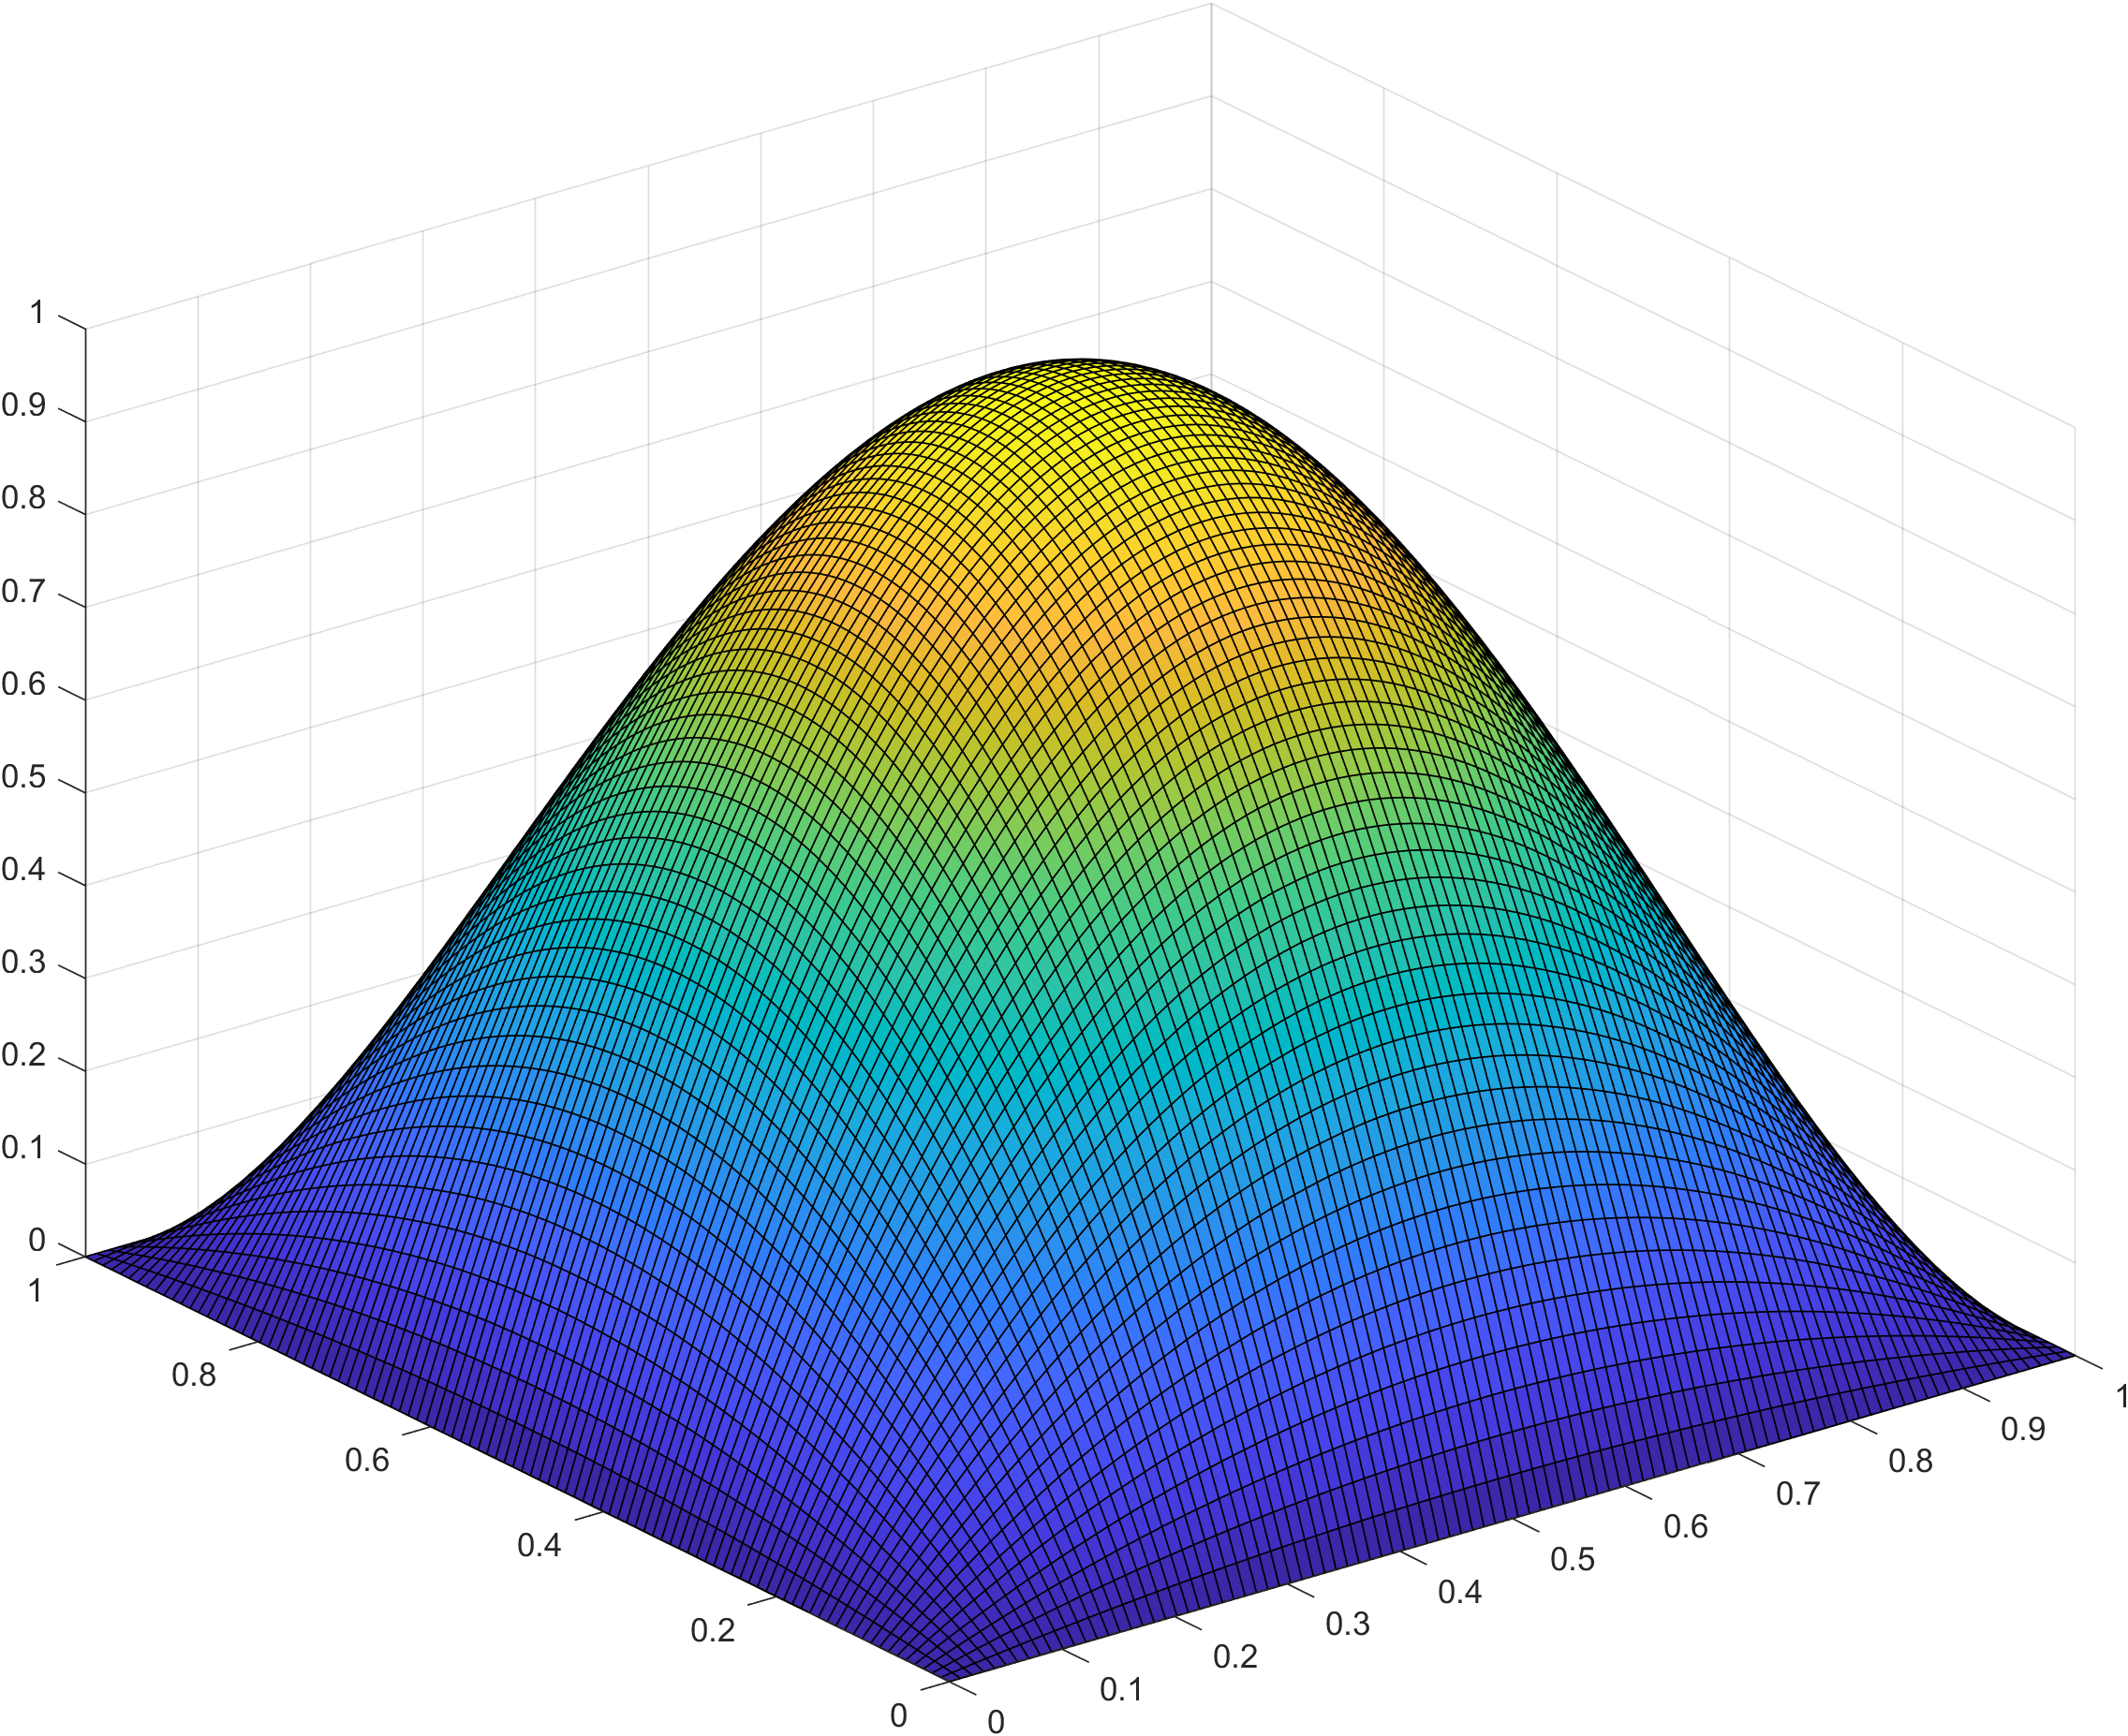
\includegraphics[height=\dimIm]{../Immagini/DO_SE_NPunti=100.png}
                    \caption{Soluzione esatta.}
                    \label{figDOTriangolazioniEsatta}
                \end{subfigure}
                \begin{subfigure}[t]{\lungSF}
                    \centering
                    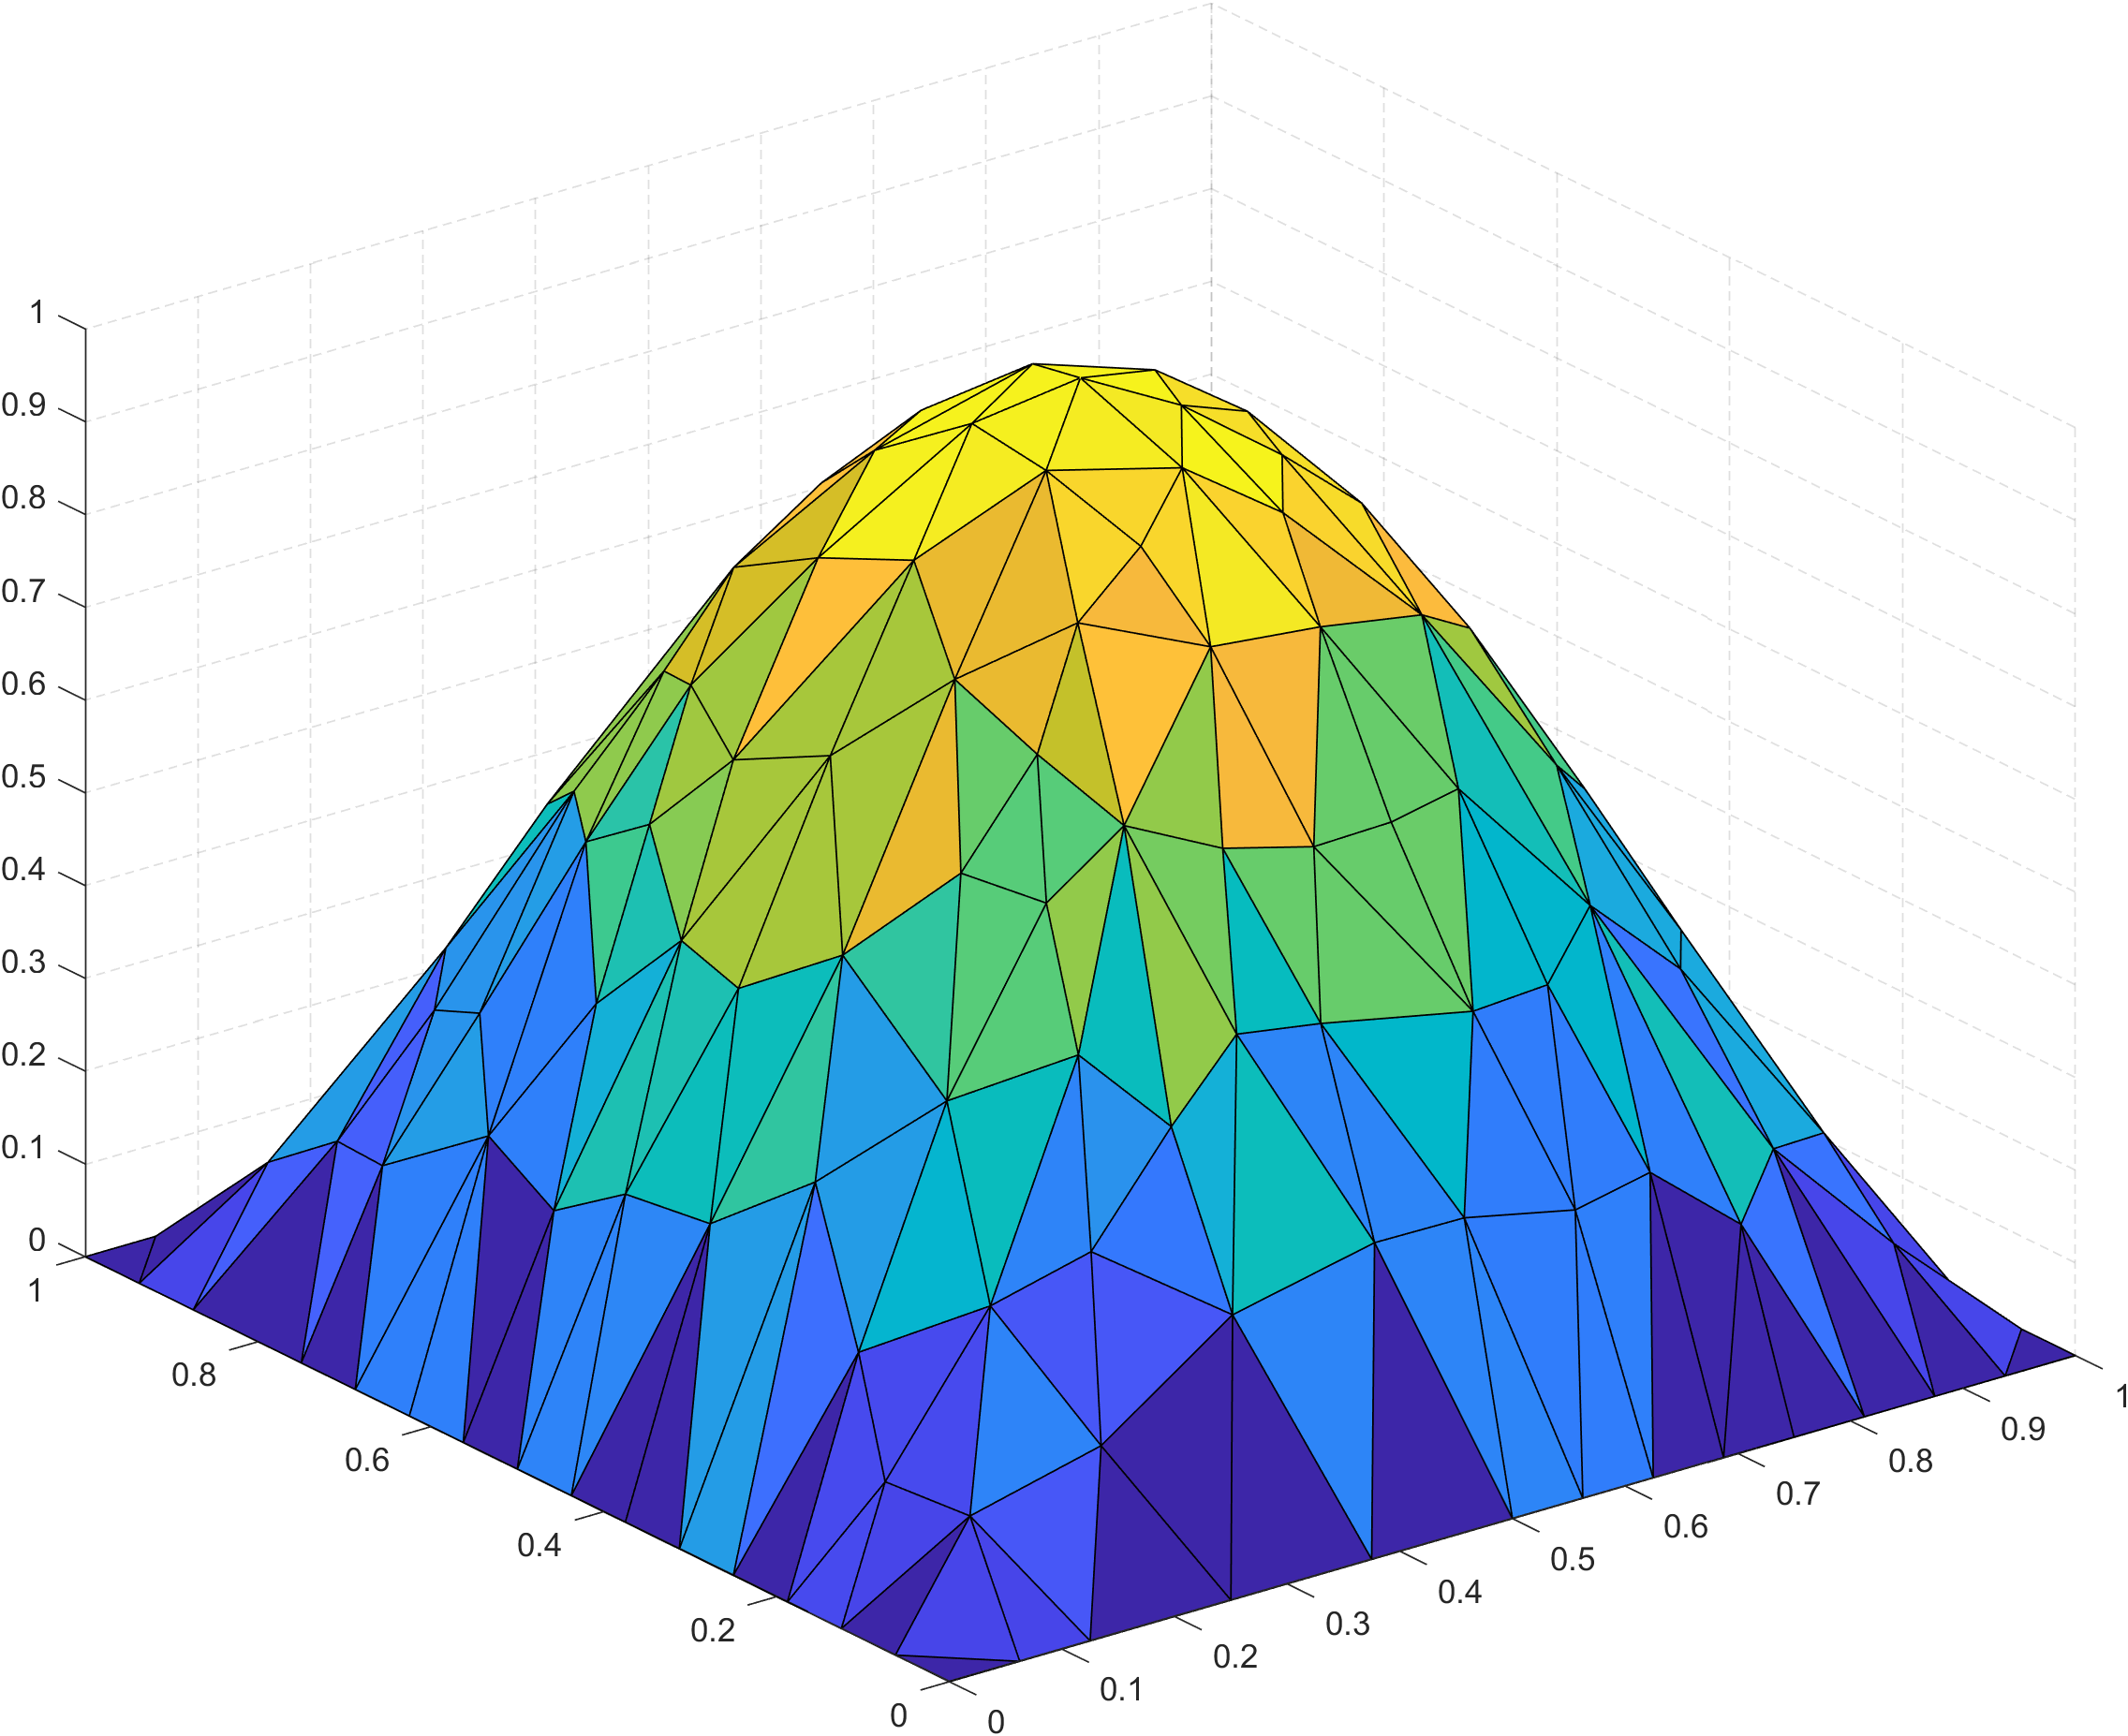
\includegraphics[height=\dimIm]{../Immagini/DO_P1_AMax=0.005.png}
                    \caption{Soluzione qualitativa coi $\mathbb{P}_1$.}
                    \label{figDOTriangolazioniApprossimataP1}
                \end{subfigure}
                \begin{subfigure}[t]{\lungSF}
                    \centering
                    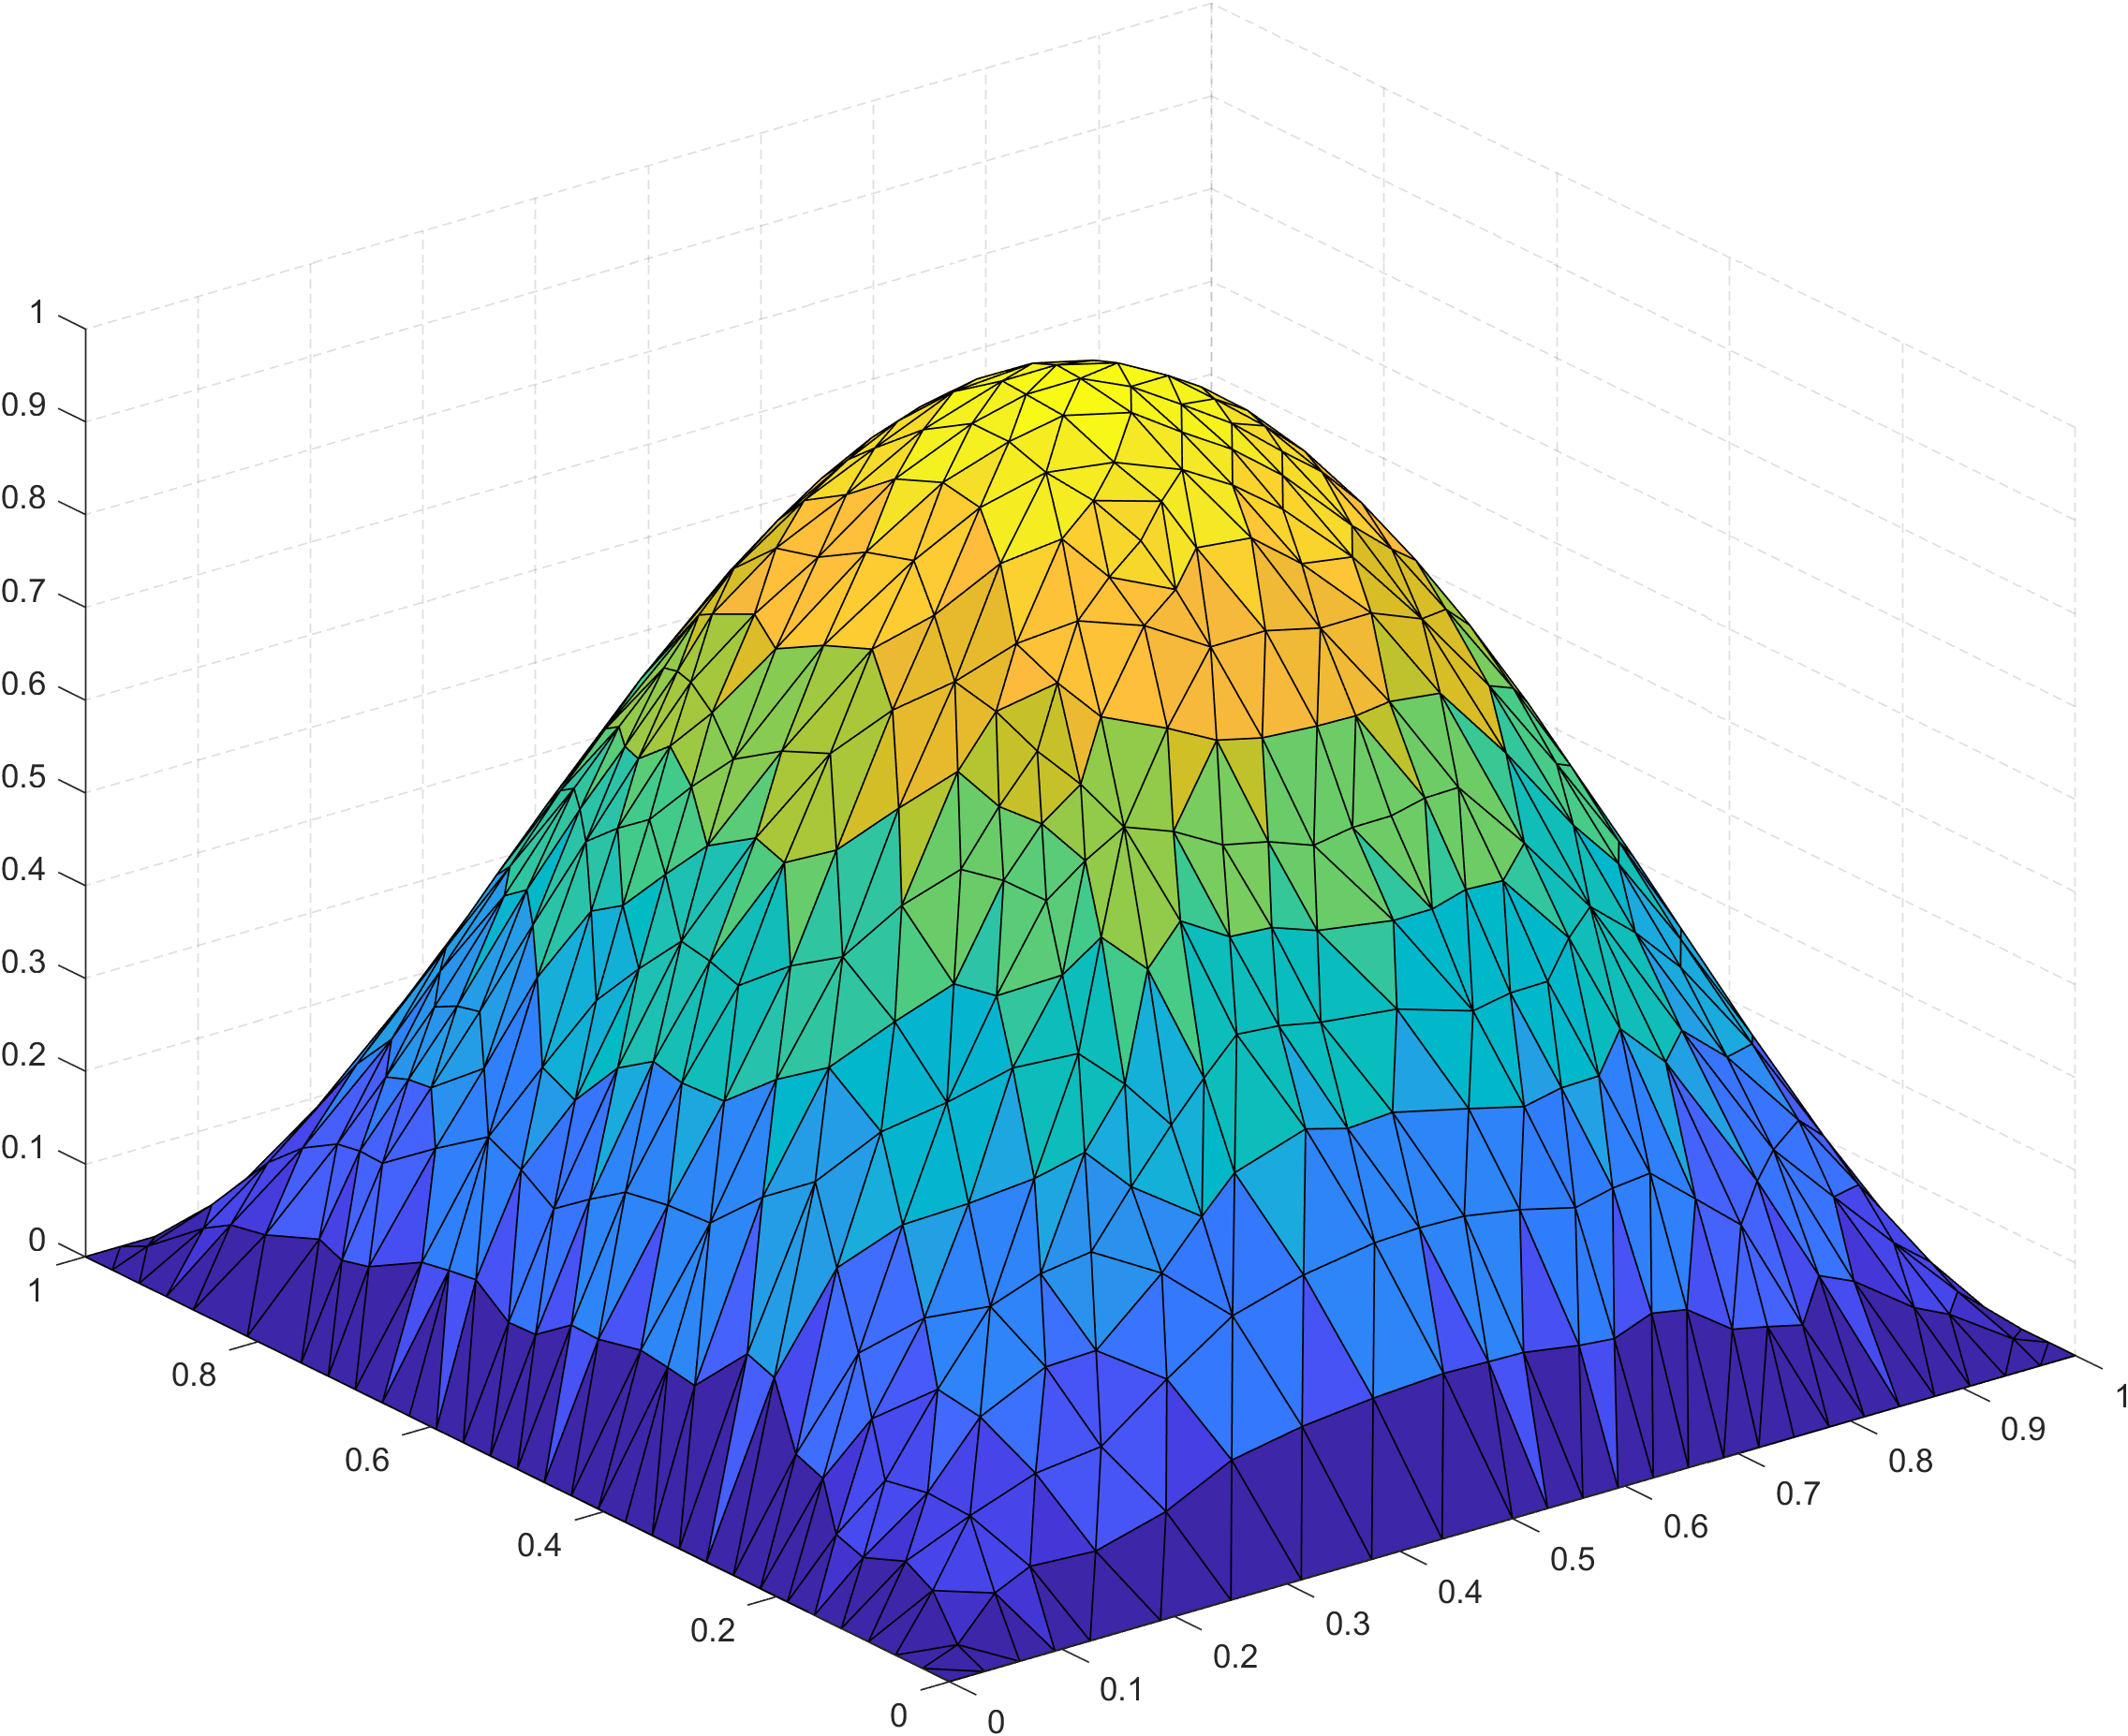
\includegraphics[height=\dimIm]{../Immagini/DO_P2_AMax=0.005.png}
                    \caption{Soluzione qualitativa coi $\mathbb{P}_2.$}
                    \label{figDOTriangolazioniApprossimataP2}
                \end{subfigure}
            }
            \distR
            
            \renewcommand{\lungSF}{.5\linewidth}
            \renewcommand{\dimIm}{.975\linewidth}
            \makebox[\linewidth][c]{
                \begin{subfigure}[t]{\lungSF}
                    \centering
                    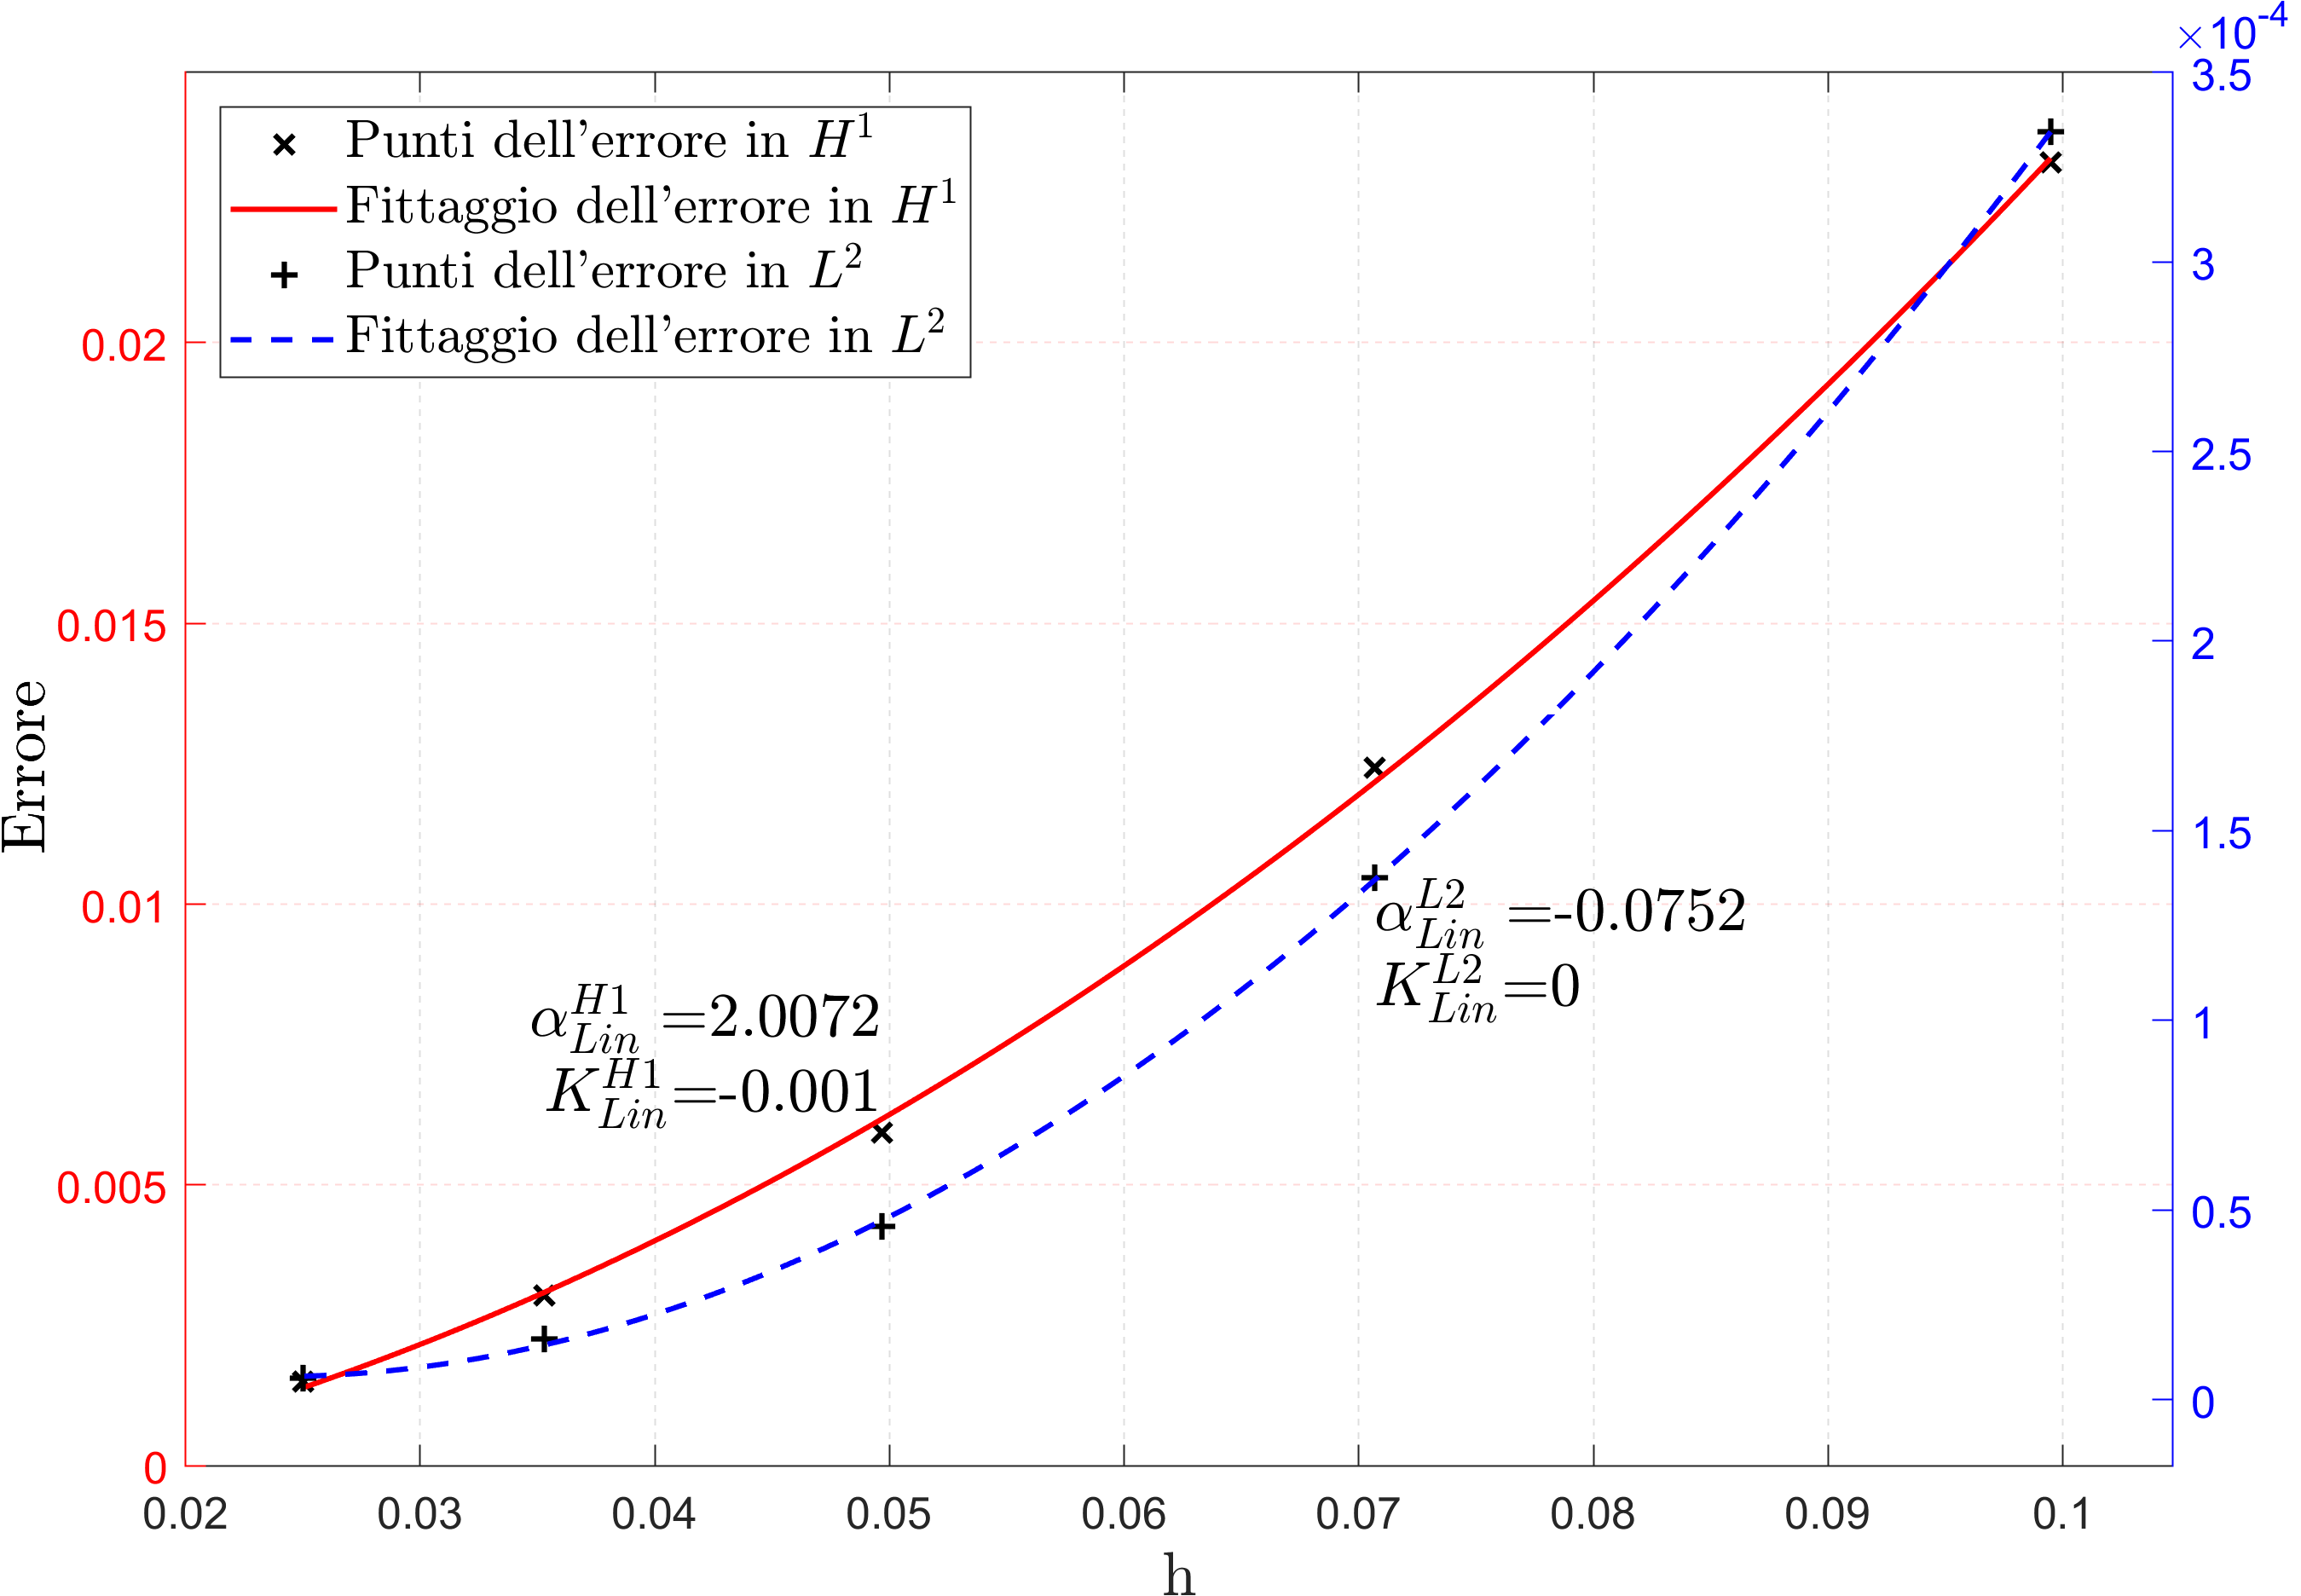
\includegraphics[width=\dimIm]{../Immagini/DO_P1_ErrLin_AMax=0.01_NSim=5.png}
                    \caption{Errore dei $\mathbb{P}_1$ in scala lineare.}
                    \label{figDOErroreP1Lin}
                \end{subfigure}
                \begin{subfigure}[t]{\lungSF}
                    \centering
                    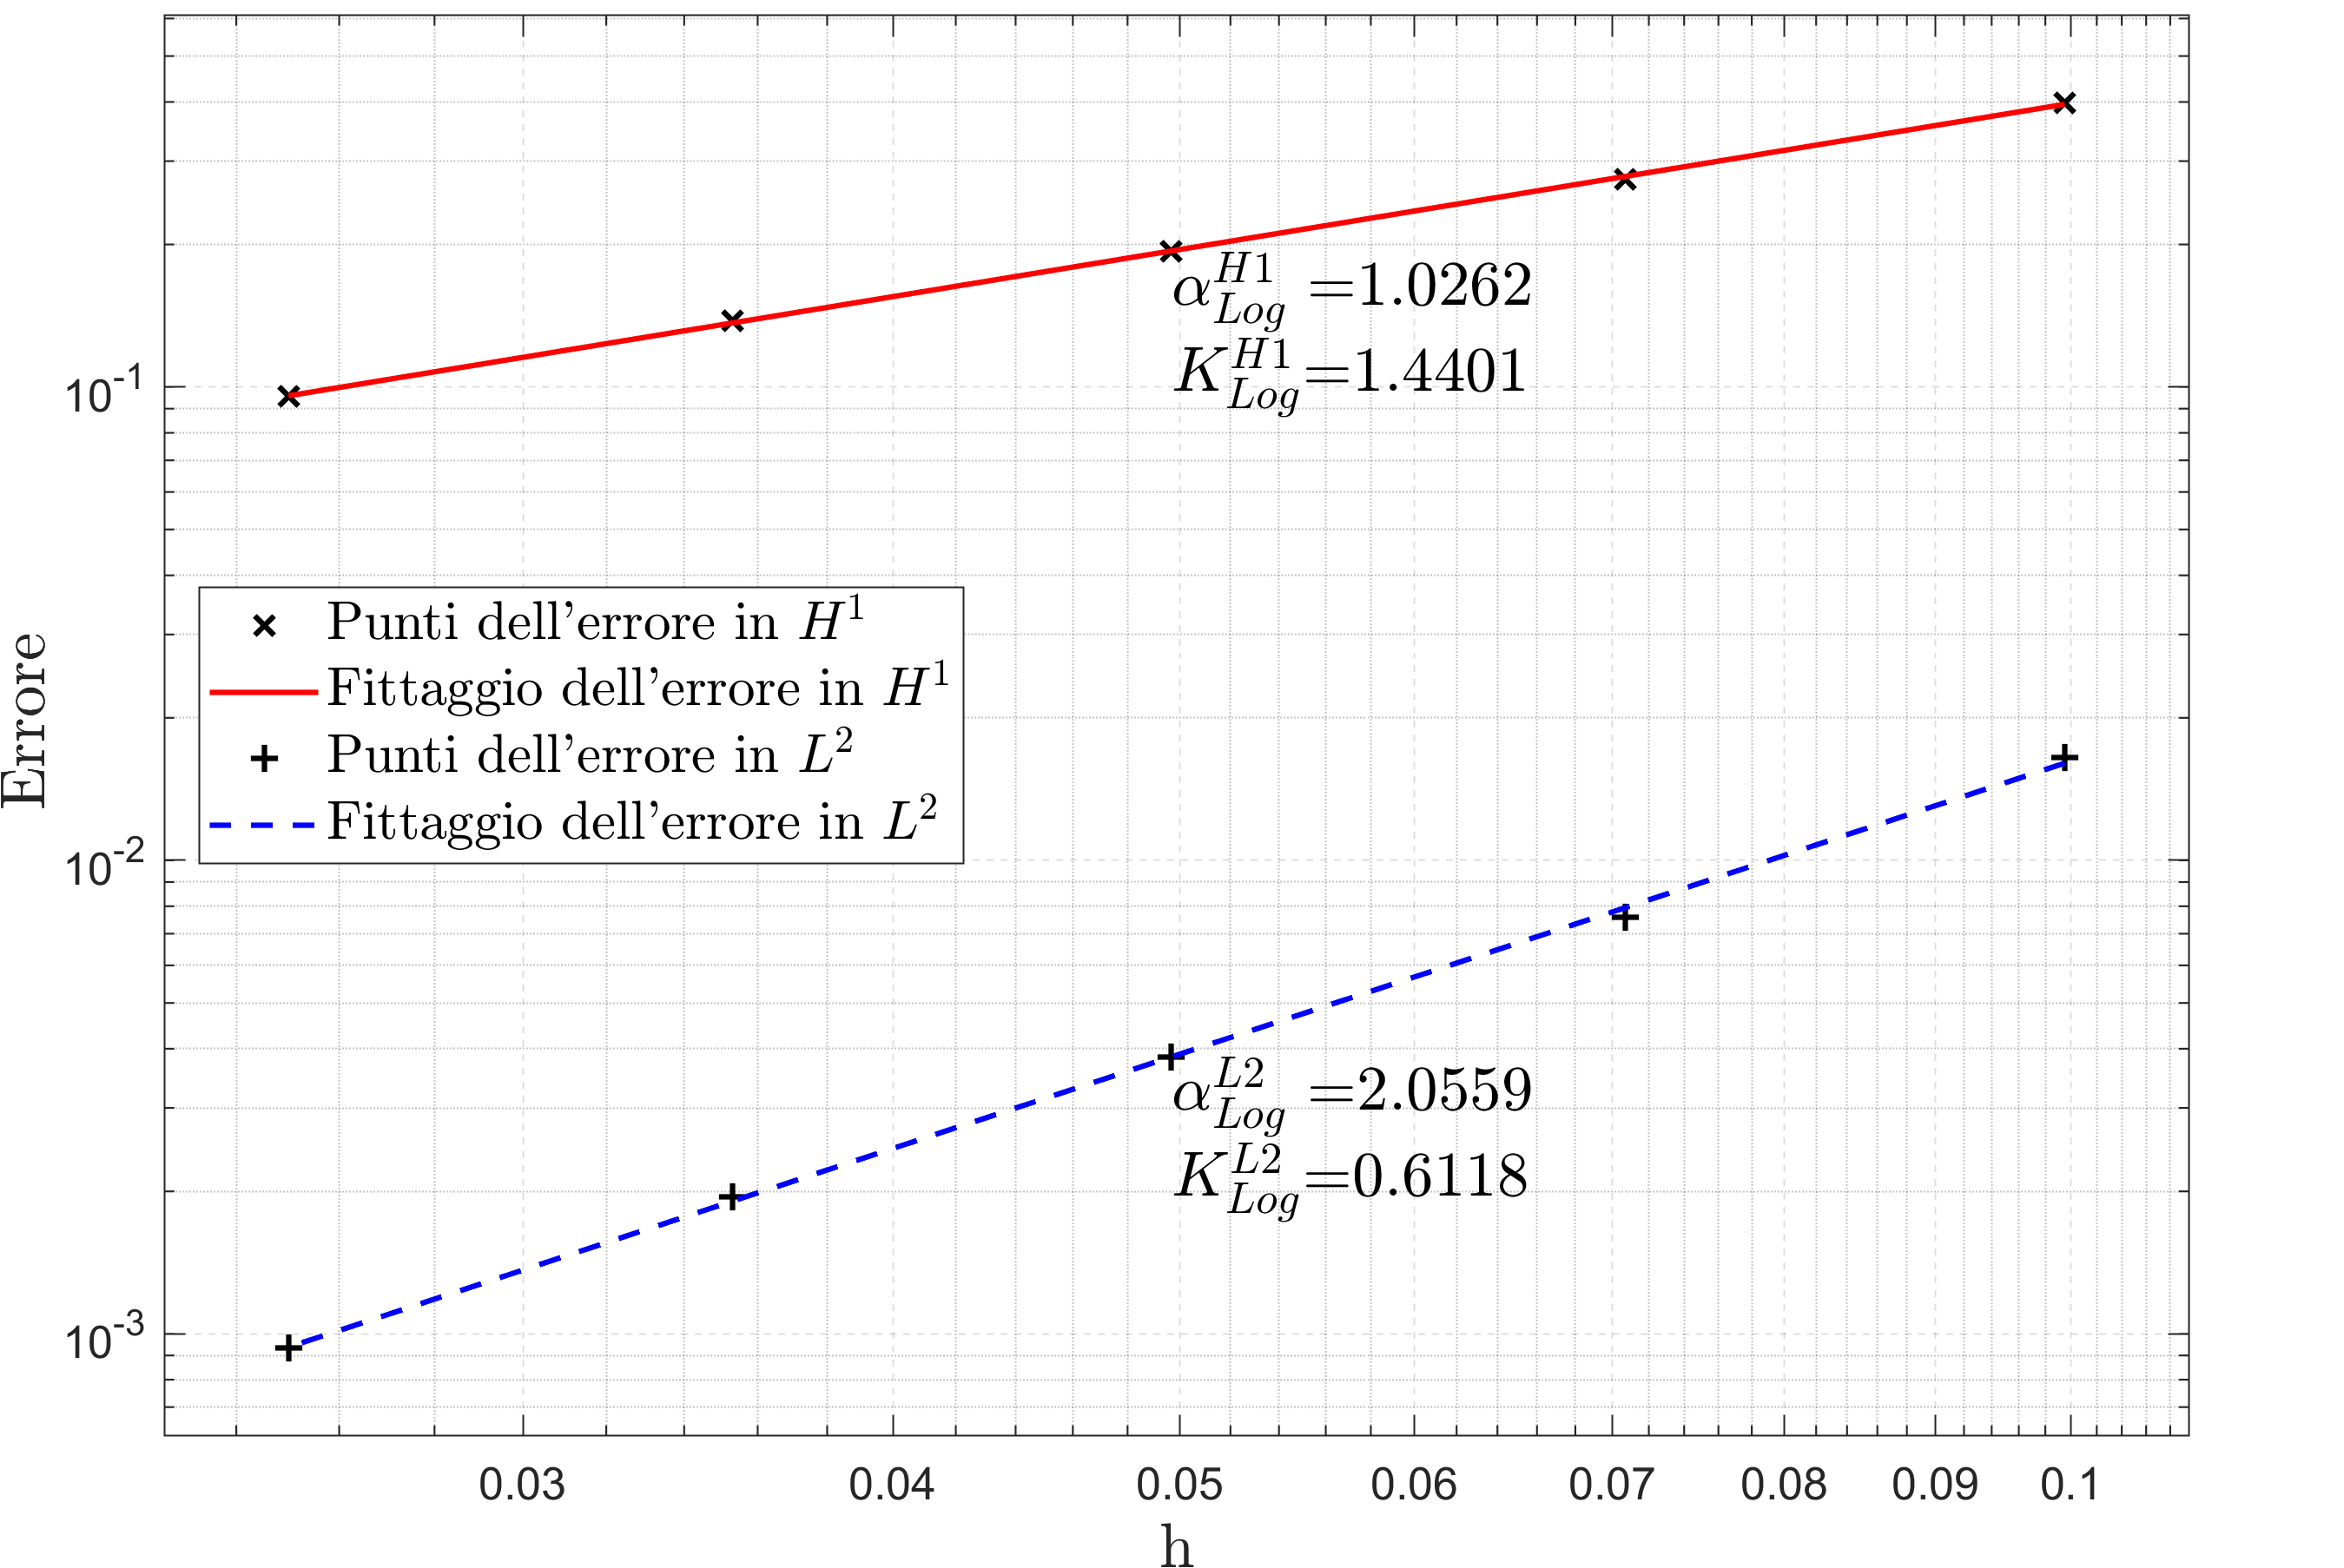
\includegraphics[width=\dimIm]{../Immagini/DO_P1_ErrLog_AMax=0.01_NSim=5.png}
                    \caption{Errore dei $\mathbb{P}_1$ in scala logaritmica.}
                    \label{figDOErroreP1Log}
                \end{subfigure}
            }
            \distR

            \makebox[\linewidth][c]{
                \begin{subfigure}[t]{\lungSF}
                    \centering
                    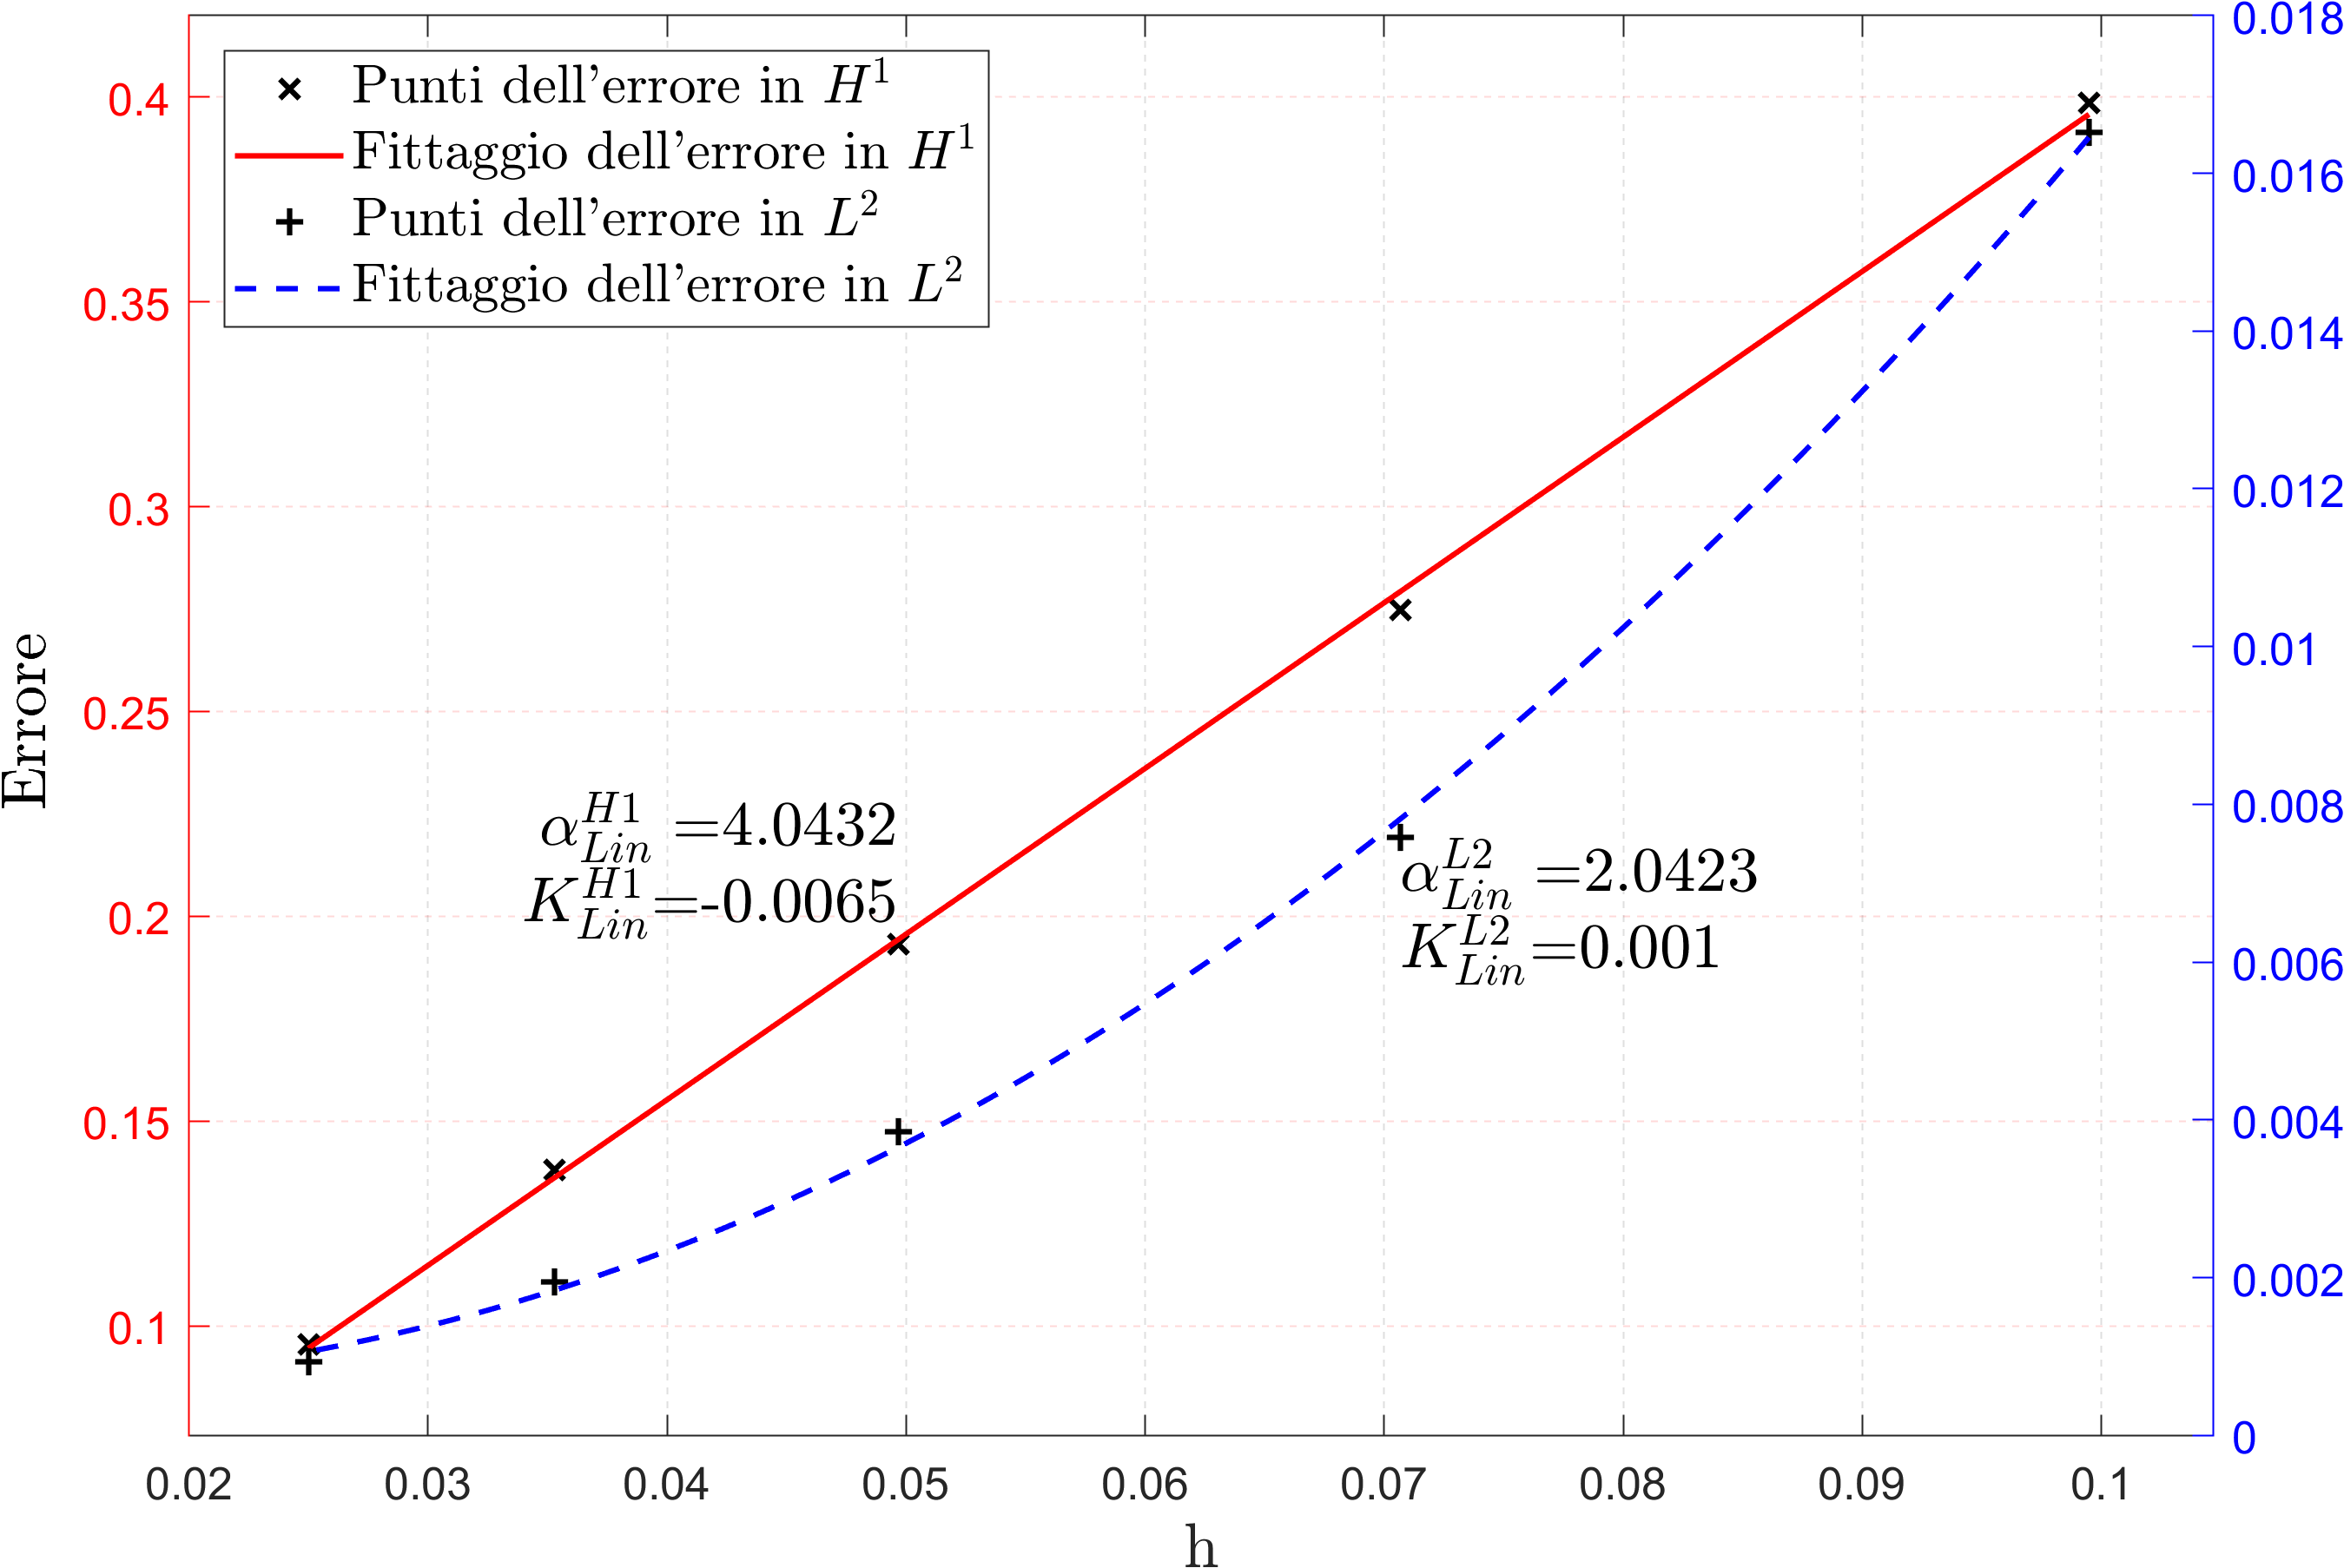
\includegraphics[width=\dimIm]{../Immagini/DO_P2_ErrLin_AMax=0.01_NSim=5.png}
                    \caption{Errore dei $\mathbb{P}_2$ in scala lineare.}
                    \label{figDOErroreP2Lin}
                \end{subfigure}
                \begin{subfigure}[t]{\lungSF}
                    \centering
                    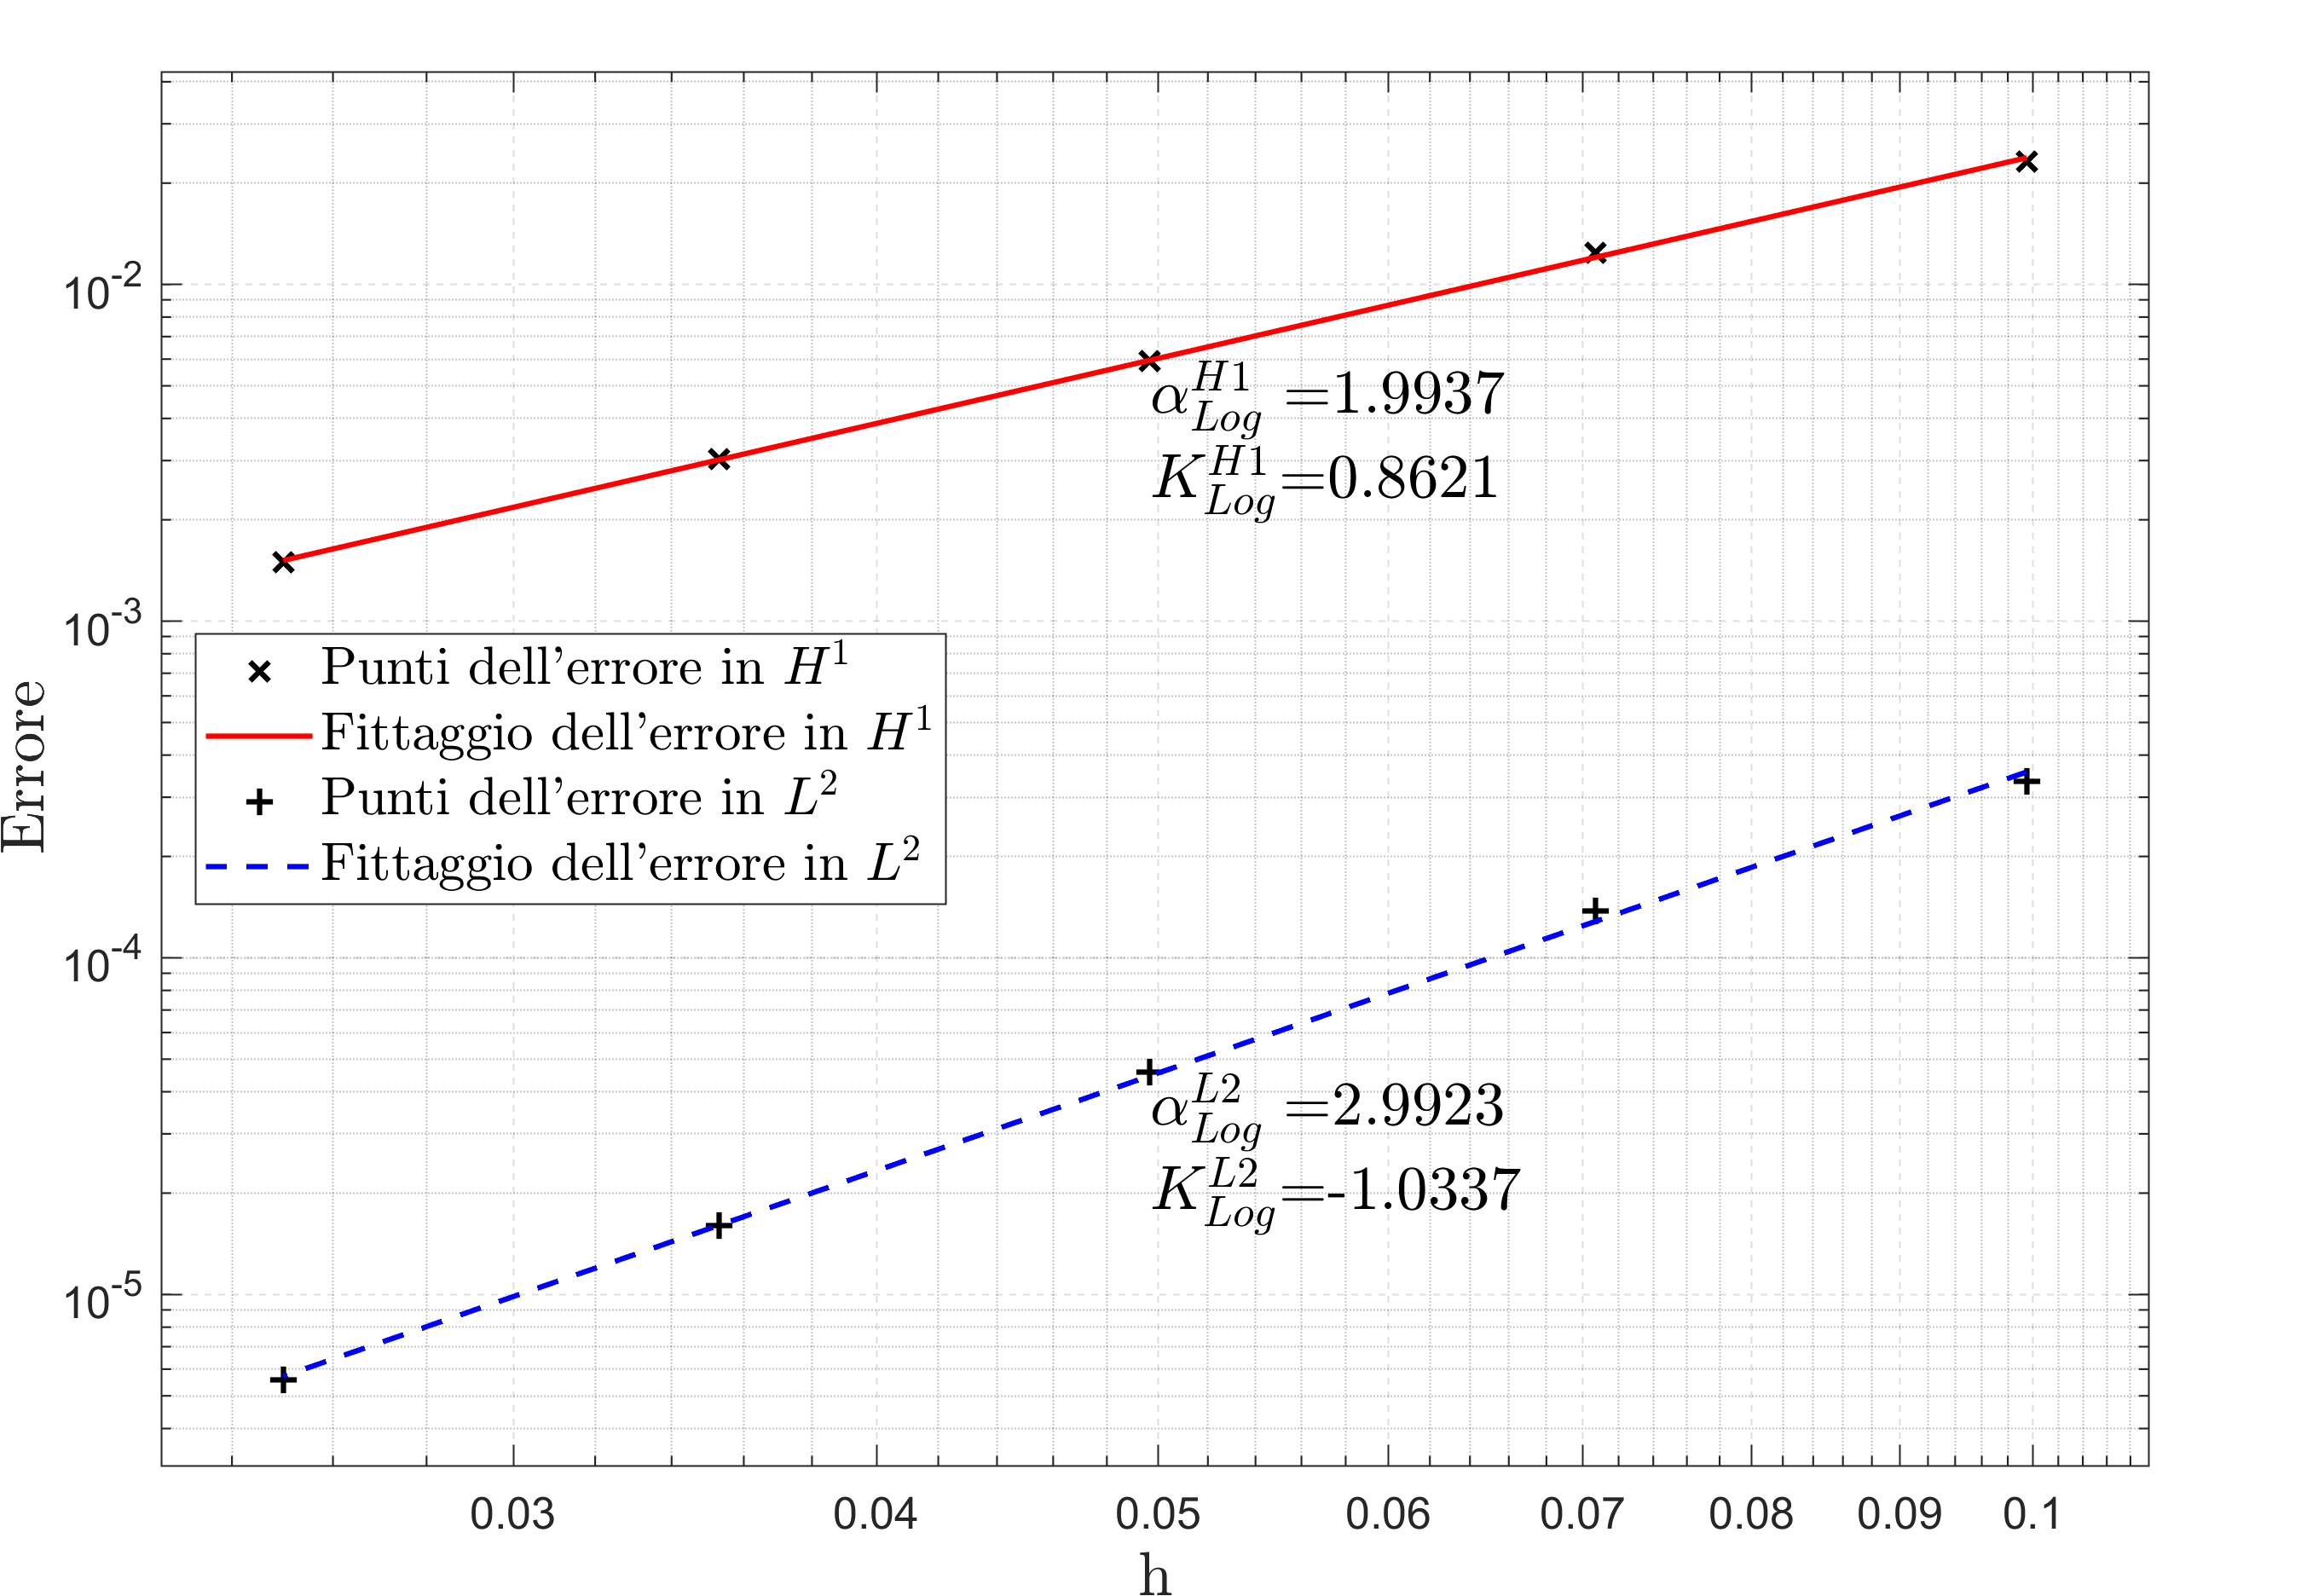
\includegraphics[width=\dimIm]{../Immagini/DO_P2_ErrLog_AMax=0.01_NSim=5.png}
                    \caption{Errore dei $\mathbb{P}_2$ in scala logaritmica.}
                    \label{figDOErroreP2Log}
                \end{subfigure}
            }
            \caption{Nelle Figg. \ref{figDOTriangolazioniEsatta}-\ref{figDOTriangolazioniApprossimataP2} sono mostrate le soluzioni del DO: una esatta e le altre approssimate; invece nelle \ref{figDOErroreP1Lin}-\ref{figDOErroreP2Log} sono illustrati in due scale diverse gli errori in norma $H^1$ ed $L^2$. I parametri dati a \textit{BBTR} sono spiegati nel $\S$\ref{parPremessaParametriBBTR}.}
            \label{figDO}
        \end{figure*}


        Prima di affrontare i vari casi di studio sono necessarie alcune premesse, ad esempio sui parametri dati a \textit{BBTR} per generare le varie triangolazioni e il programma usato per scrivere il codice.

        
        \subsection{Premesse sull'implementazione}\label{parPremessaParametriBBTR}

            In primo luogo l'unicità della soluzione dimostrata dal Teorema di Lax-Milgram implica che porre condizioni di Dirichlet o di Neumann è del tutto equivalente [sotto certe condizioni (si v. \cite{dispenseMEDèPA} Esempio 1.2.2 a p. 15 per maggiori dettagli)]; lo stesso varrà per gli ordini di convergenza, ragion per cui nei casi di studio a seguire si porranno solo condizioni di Dirichlet, vale a dire
            %
            \begin{equation*}
                \Gamma_D=\partial\Omega\ \ \text{e}\ \Gamma_N=\emptyset,
            \end{equation*}
            %
            mentre quelle di Neumann saranno prese in considerazione esclusivamente per qualche osservazione.
    
            In secondo luogo l'angolo minimo di ogni sottoinsieme $T$ degli EF è sempre stato imposto uguale a $20^\circ$.
    
            In terzo luogo l'area massima consentita per ogni EF è il parametro che identificherà la sequenza $\{\mathcal T_h\}_h$ necessaria alla valutazione dell'errore: considerando un valore di area massima di riferimento iniziale $\overline A$, è possibile generare da essa una sequenza dimezzando a ogni iterazione il valore precedente; in formule questo consiste nel prendere i primi $N$ valori della successione
            %
            \begin{equation*}
                \{A_n\}_{n\in\mathbb N}: A_n=\overline A2^{-n};
            \end{equation*}
            %
            dopo, \textit{a posteriori}, una volta generata la triangolazione $\mathcal T_{h_n}$ associata ad $A_n$, si ricava il parametro di discretizzazione mediante la radice dell'area massima effettiva fra tutti i triangoli, ovvero
            %
            \begin{equation*}
                \{h_n\}_{n\in\mathbb N}:h_n=\sqrt{\max_{T\in\mathcal T_n}\left(A_T\right)}.
                % \label{eqParametroDiscretizzazione}
            \end{equation*}
            %
            Supponendo tuttavia di porre [impropriamente] $h_n=\sqrt{\overline A2^{-n}}$, curiosamente tale scelta porta ad avere in scala logaritmica intervalli equispaziati tra gli $h_n$:
            %
            \begin{equation}
                \setlength{\thinmuskip}{1mu}
                \setlength{\medmuskip}{2mu}
                \setlength{\thickmuskip}{3mu}
                \begin{aligned}
                    \Delta h&\equiv\vert\ln(h_{n+1})-\ln(h_n)\vert\\
                    &=\frac12\vert\ln(\overline A2^{-(n+1)})-\ln(\overline A2^{-n})\vert\\
                    &=\frac12\vert\ln(\overline A)-(n+1)\ln(2)-\ln(\overline A)+n\ln(2)\vert\\
                    &=\frac12\vert-\ln(2)\vert=\frac12\ln(2).\\
                \end{aligned}
                \label{eqDimIntervalliEquispaziatiScalaLog}
            \end{equation}
            %
            E sebbene tale ragionamento non sia corretto per i valori esatti di $h_n$, lo è comunque da un punto di vista qualitativo siccome vale 
            %
            \begin{equation*}
                A_n\approx\max_{T\in\mathcal T_n}\left(A_T\right).
            \end{equation*}
            %    
            Un simile discorso continua a rimanere valido per la valutazione dell'errore in tempo collo schema di Crank-Nicolson, ove ora $\overline A$ è fisso mentre cambia il passo temporale seguendo la medesima logica delle aree: si prendono i primi $N$ termini della successione
            %
            \begin{equation*}
                \{\Delta t_n\}_{n\in\mathbb N}:\Delta t_n=\overline{\Delta t}2^{-n}.
            \end{equation*}
            %
            In tutti i casi di studio a seguire, si porrà $\overline A=\overline{\Delta t}=0.01$ ed $N=5$ per la valutazione dell'errore (p. es. le Figg. \ref{figDOErroreP1Lin}-\ref{figDOErroreP2Log}), mentre per le approssimazioni qualitative della soluzione (p. es. le Figg. \ref{figDOTriangolazioniApprossimataP1} e \ref{figDOTriangolazioniApprossimataP2}) si ha $\overline A=\overline{\Delta t}=0.005$ ed $N=1$.
            
            Inoltre vi sono due osservazioni sui grafici degli errori:
    
            \begin{enumerate}[label=\arabic*.,    % Cambia l'etichetta degli elementi («item»)
                              itemsep=0pt,        % Spazio tra gli elementi («item») della lista
                              leftmargin=12.5pt]    % Spazio tra la lista e il bordo destro del testo
            
                \item Poiché l'errore calcolato in norma $L^2$ è molto inferiore rispetto a quello in $H^1$, in scala lineare sono stati usati due assi delle ordinate: rosso per l'errore in $H^1$ (linea continua) e blu per l'errore in $L^2$ (linea tratteggiata).
                
                \item I due coefficienti $\alpha$ e $K$ [a fianco delle curve] indicano rispettivamente il coefficiente moltiplicato al monomio di grado massimo\footnote{Se è una retta corrisponde al coefficiente angolare, altrimenti è il coefficiente moltiplicato a $x^2$ per una parabola, a $x^3$ per una cubica e cosí via.} e l'intercetta del polinomio fittante.
    
            \end{enumerate}
    
            Infine il programma usato per l'implemetanzione è MATLAB versione «24.2.0.2773142 (R2024b) Update 2».

        
        \subsection{Dirichlet omogeneo (DO)}

            Esso consiste in un problema con condizioni al bordo di Dirichlet omogenee ($g_D=0$) e con sola diffusione, ovvero
            %
            \begin{equation*}
                \setlength{\abovedisplayskip}{5pt plus 2pt minus 2pt}  % Riduce lo spazio sopra l'equazione
                \setlength{\belowdisplayskip}{5pt plus 2pt minus 2pt}  % Riduce lo spazio sotto l'equazione
                \SpaziaturaMate{1}{2}{3}
                \nu=1,\;\;\beta=(0,0)^{\top}\text{ e }\sigma=0;
            \end{equation*}
            %
            il che equivale a trasformare il \teqref{eqProblemaStazionario}{[PS]} in
            %
            \begin{equation}
                \left\{
                \begin{aligned}
                    -\Delta u&=f&\text{in }&\Omega, \\
                            u&=0&\text{su }&\partial\Omega,
                \end{aligned}
                \right.
                \label{eqDO}
            \end{equation}
            %
            ove s'impone che la soluzione esatta $u$ sia pari a
            %
            \begin{equation*}
                u=16x(1-x)y(1-y).
                \label{eqSoluzioneEsattaDO}
            \end{equation*}
            %
            Nella Fig. \ref{figDOTriangolazioniEsatta} è mostrata la soluzione esatta mentre nelle Figg. \ref{figDOTriangolazioniApprossimataP1} e \ref{figDOTriangolazioniApprossimataP2} le due approssimate mediante i $\mathbb P_1$ e i $\mathbb P_2$ rispettivamente. D'altro canto nelle Figg. \ref{figDOErroreP1Lin} e \ref{figDOErroreP1Log} è illustrato l'andamento dell'errore per i $\mathbb P_1$ e similmente nelle Figg. \ref{figDOErroreP2Lin} e \ref{figDOErroreP2Log} per i $\mathbb P_2$ (i relativi dati si trovano nella Tab. \ref{tabErroriDO}); questi andamenti corrispondono a quanto detto nel $\S$\ref{parAnalisiErrore}.

            In questo caso di studio è anche notevole osservare che il bordo \textit{non} può essere solo di Neumann ($\SpaziaturaMate{1}{2}{3}\Gamma_N=\partial\Omega\ \ \text{e}\ \Gamma_D=\emptyset$); infatti in tali condizioni si perde la coercività della forma bilineare descritta dalla \eqref{eqOperatoreBilinearePSVariazionale} visto che vale la contraddizione
            %
            \begin{equation*}
                0=\sigma=-\frac 12\nabla\cdot\boldsymbol\beta+\sigma\ge\sigma_0>0,
            \end{equation*}
            %
            con $\sigma_0$ costante positiva (si v. \cite{dispenseMEDèPA} Esempio 1.2.2 a p. 17 per maggiori dettagli); dalle Figg. \ref{figDOEsplodenteP1} e \ref{figDOEsplodenteP2}, ciò non fa esplodere la soluzione, la quale rimane stabile seppure sbagliata sia per i $\mathbb P_1$ che per i $\mathbb P_2$.

            %%% Questa figura appartiene al prossimo paragrafo %%%
            \begin{figure*}[t]
                \newcommand{\lungSF}{0.33\textwidth}
                \newcommand{\dimIm}{4cm}
                \makebox[\linewidth][c]{
                    \begin{subfigure}[t]{\lungSF}
                        \centering
                        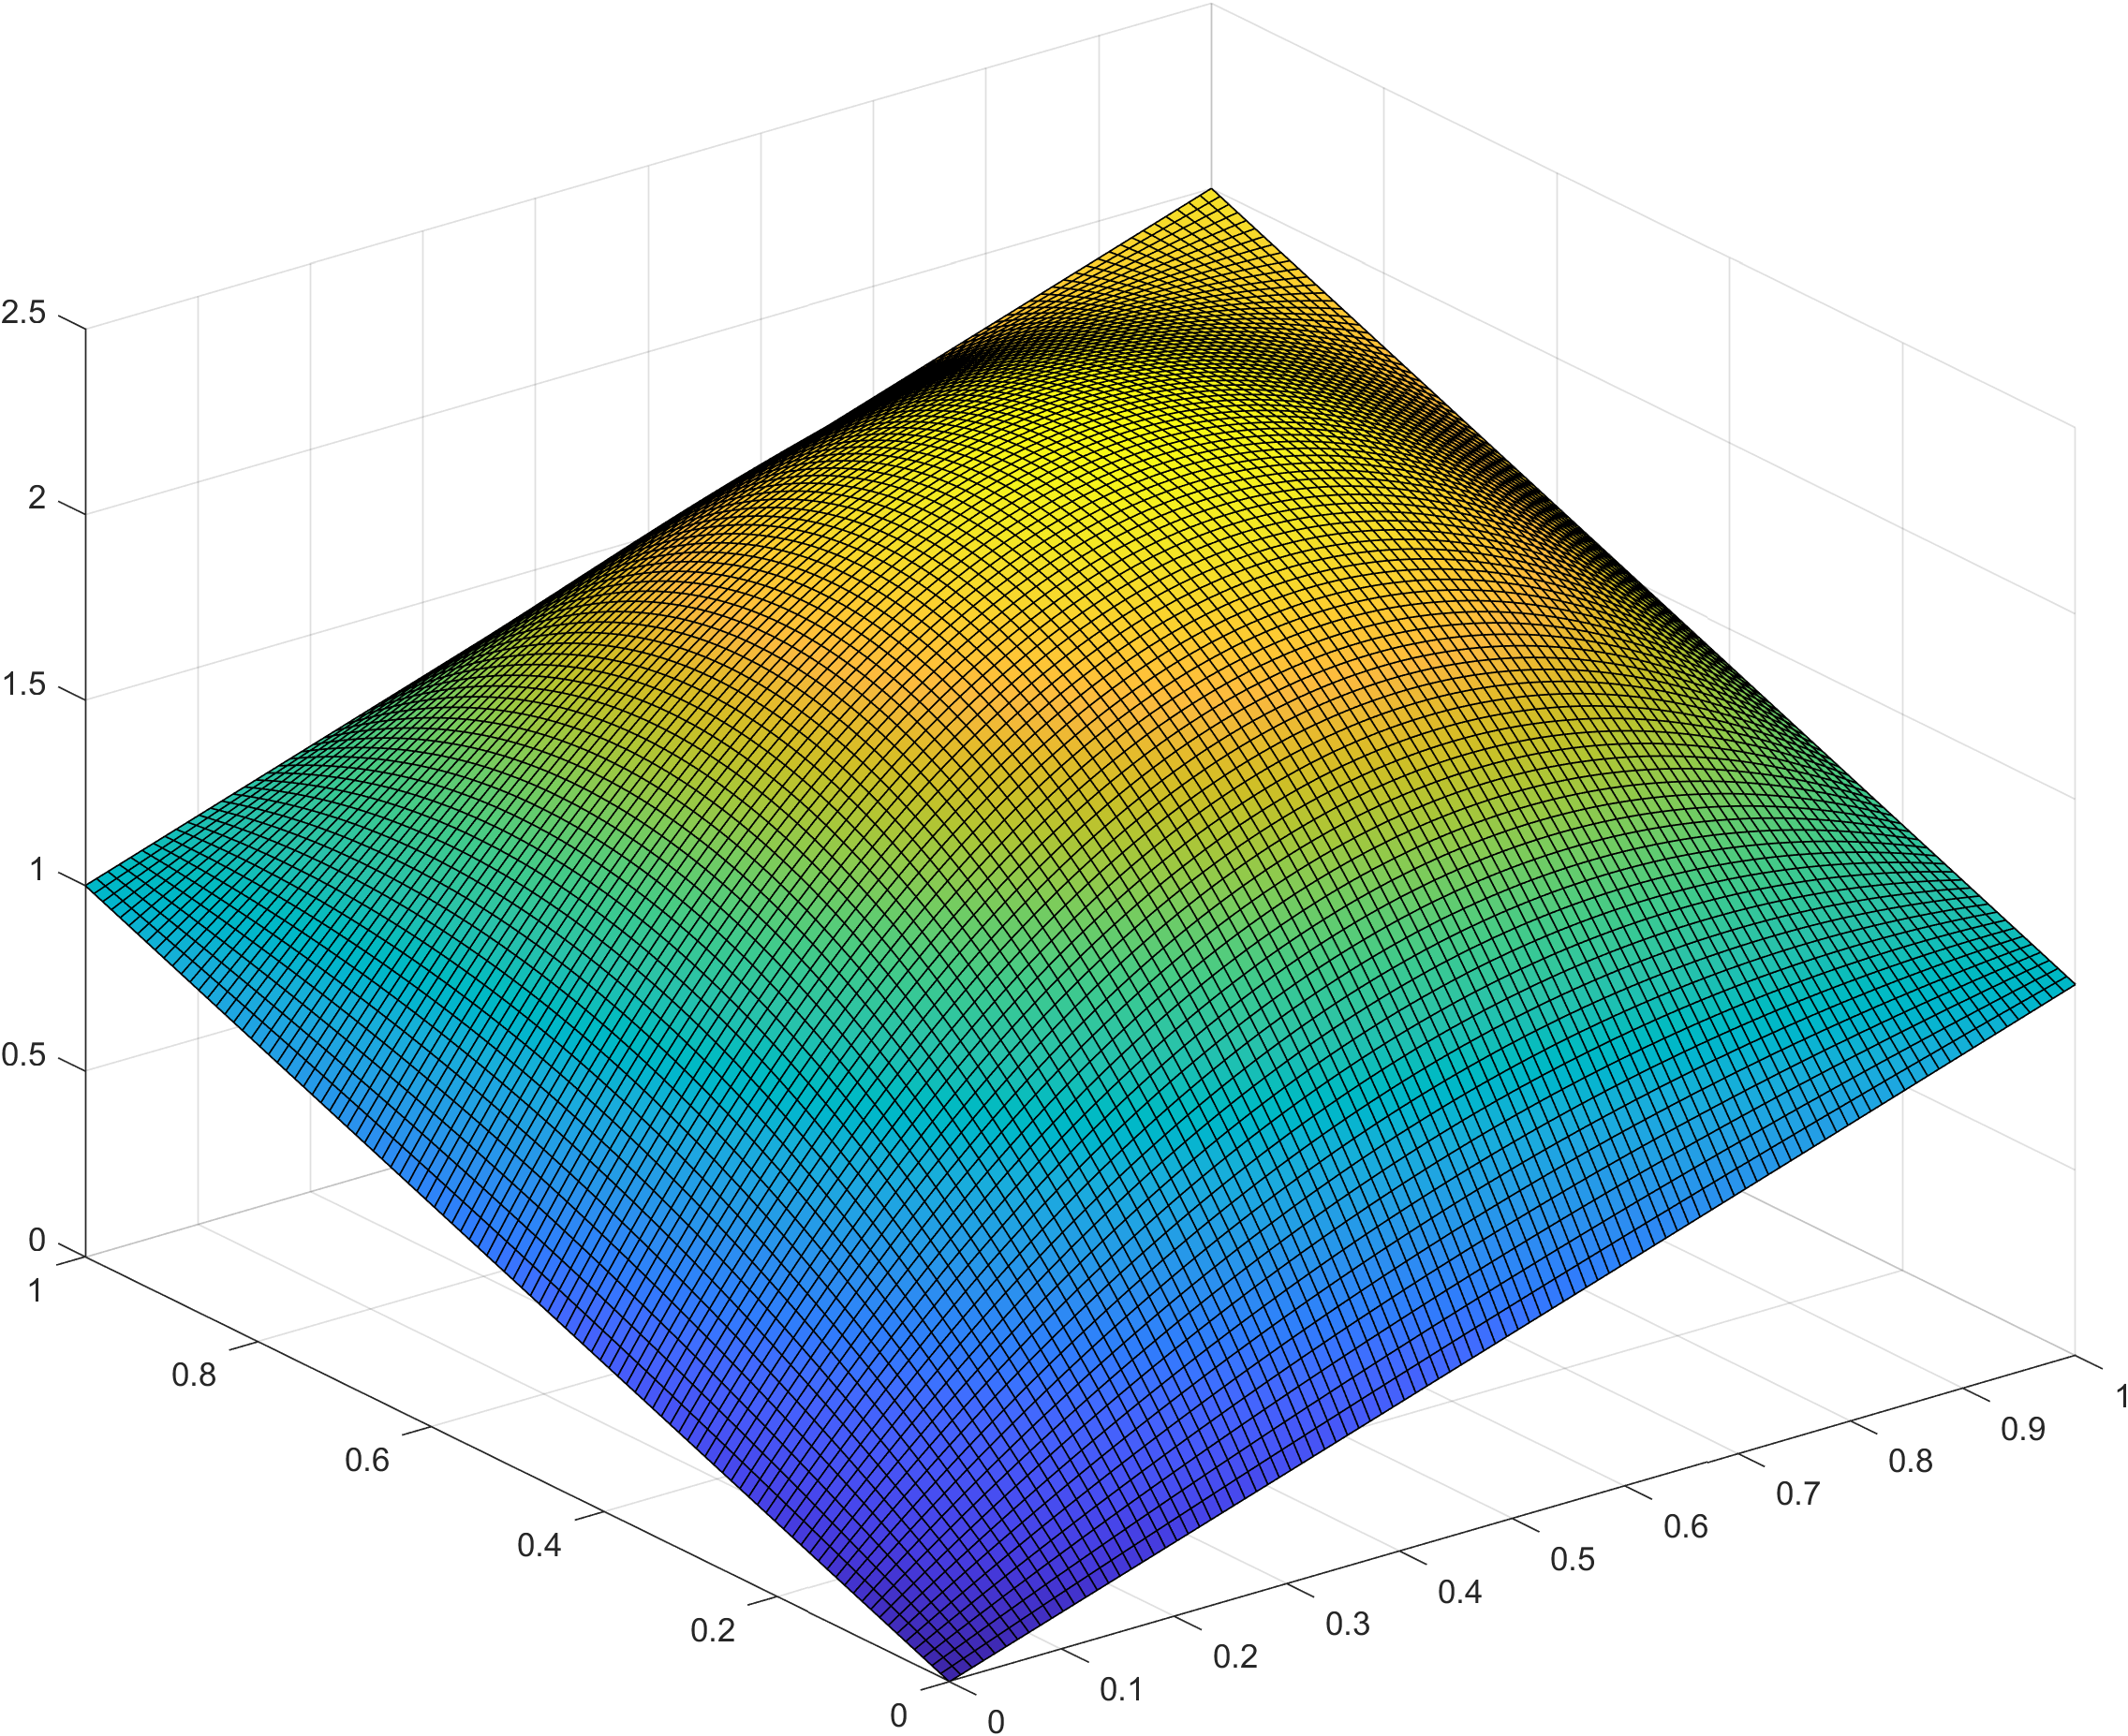
\includegraphics[height=\dimIm]{../Immagini/DNO_SE_NPunti=100.png}
                        \caption{Soluzione esatta.}
                        \label{figDNOTriangolazioniEsatta}
                    \end{subfigure}
                    \begin{subfigure}[t]{\lungSF}
                        \centering
                        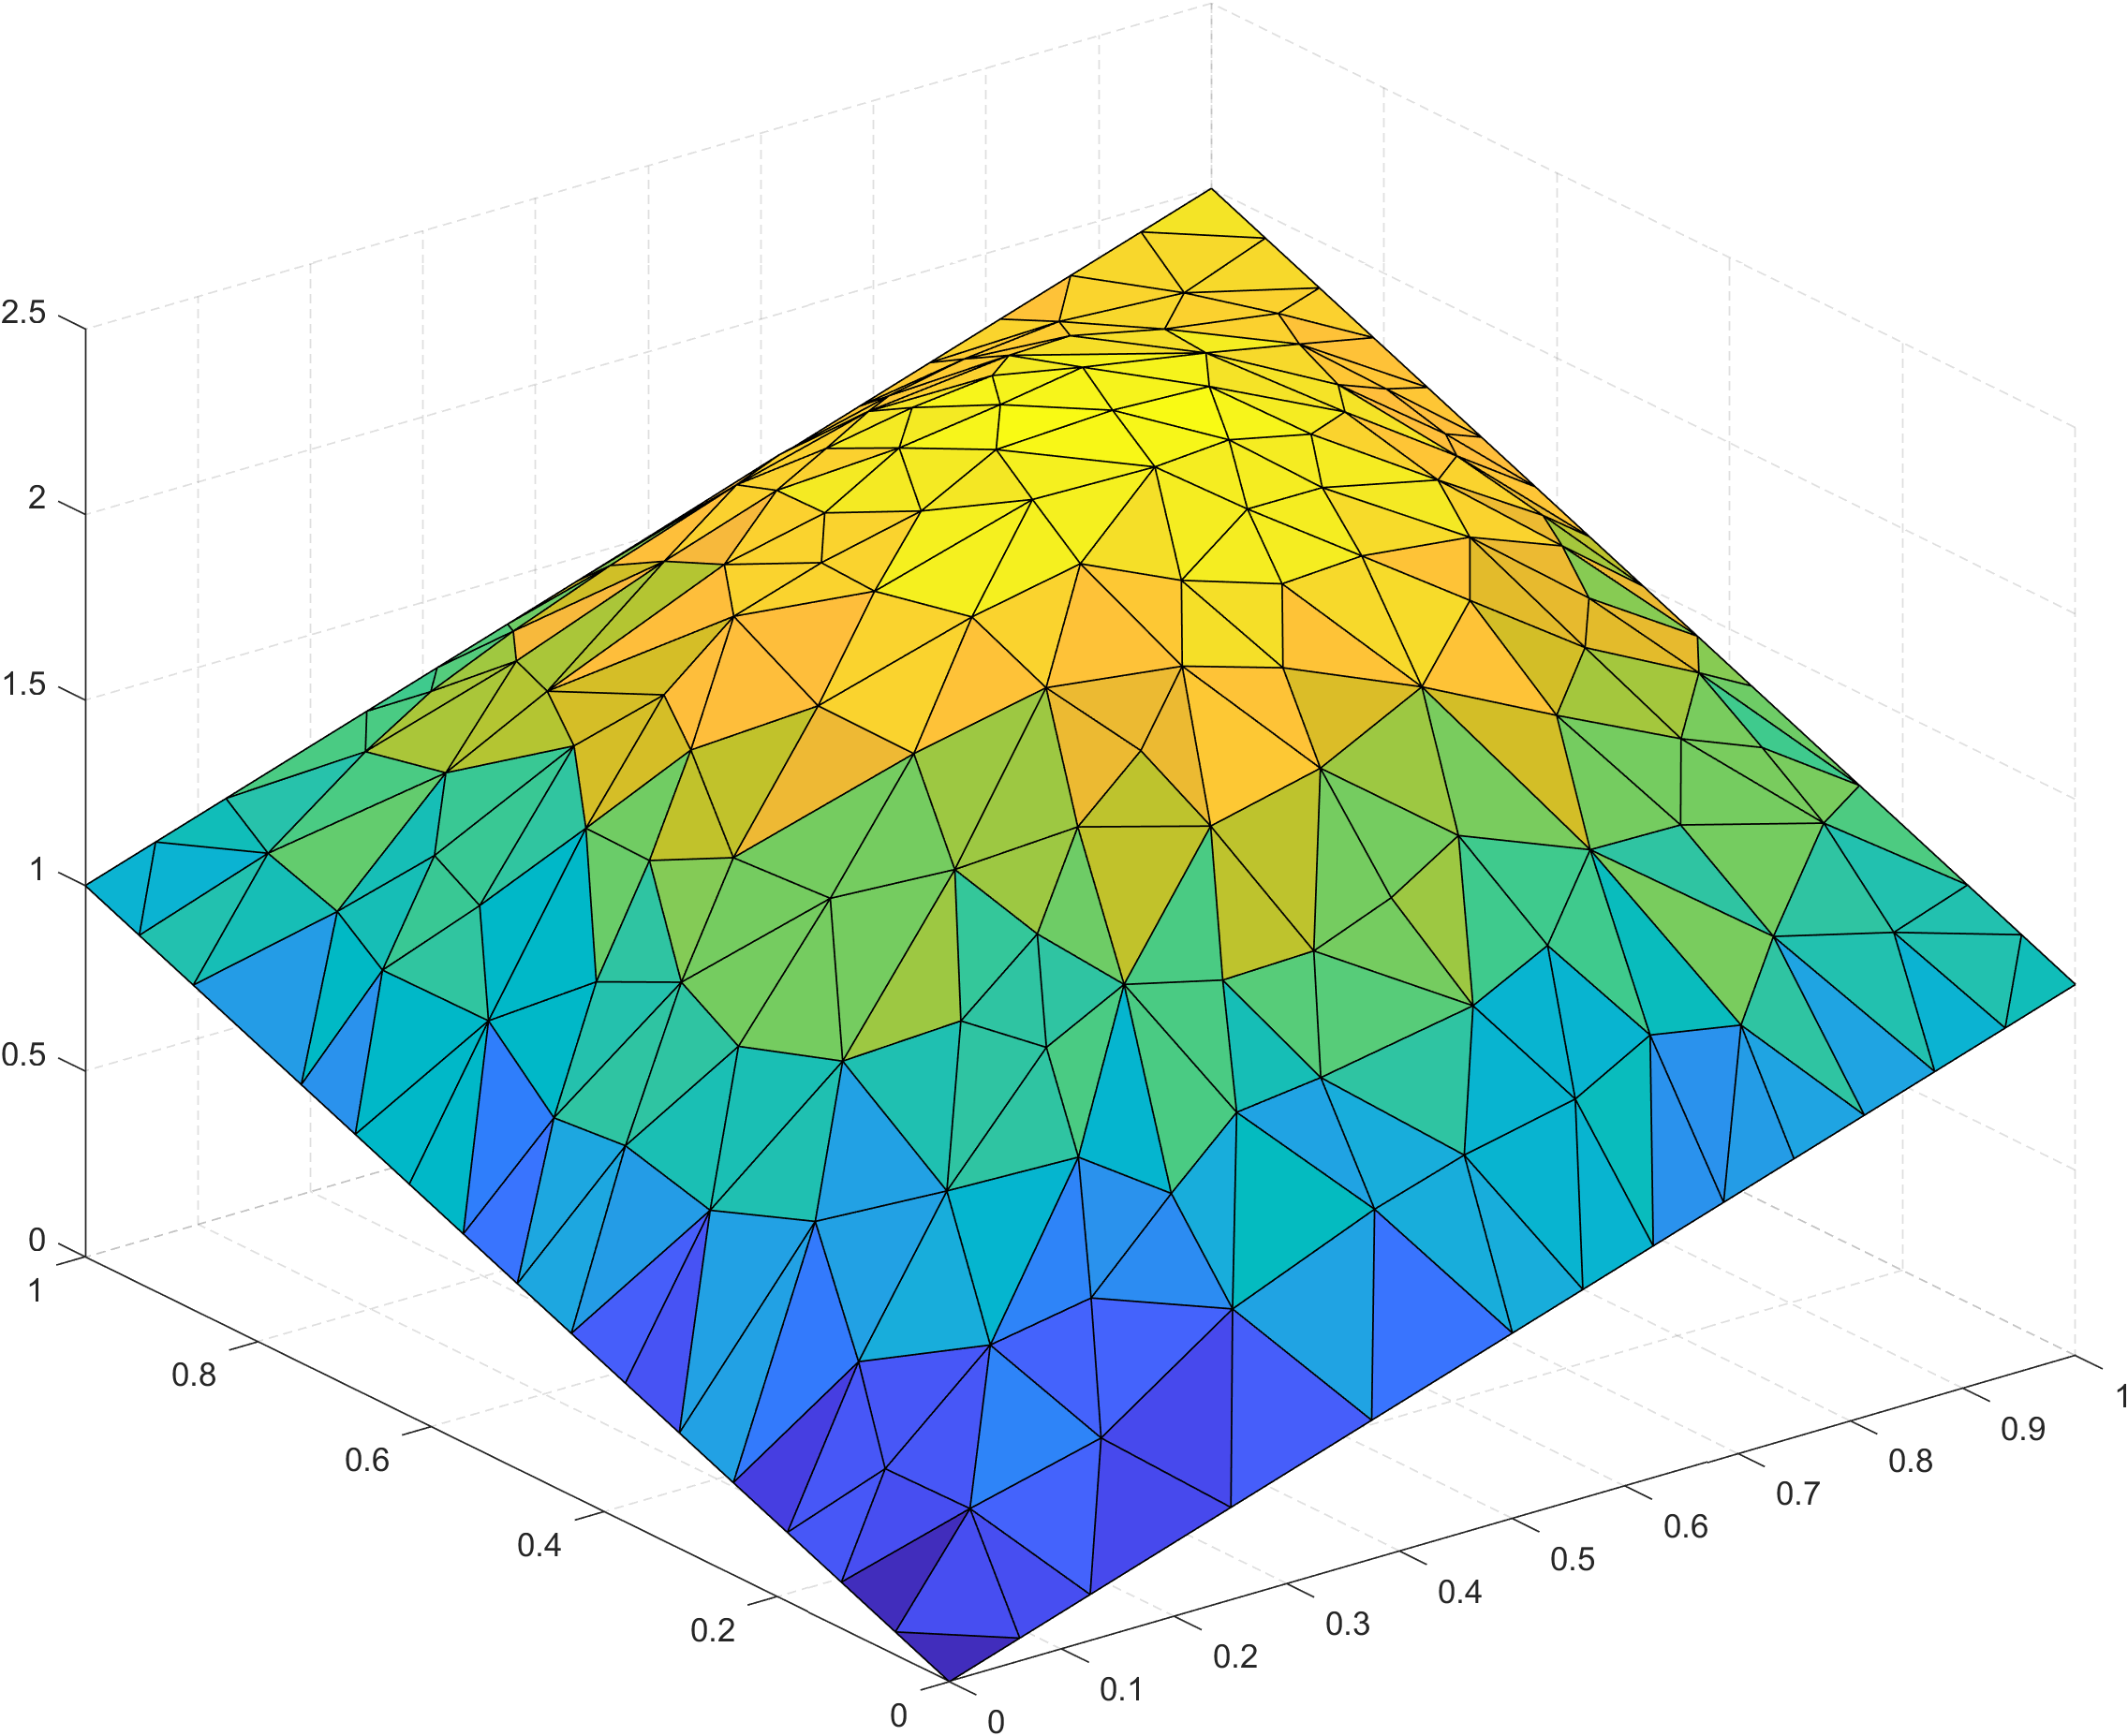
\includegraphics[height=\dimIm]{../Immagini/DNO_P1_AMax=0.005.png}
                        \caption{Soluzione qualitativa coi $\mathbb{P}_1$.}
                        \label{figDNOTriangolazioniApprossimataP1}
                    \end{subfigure}
                    \begin{subfigure}[t]{\lungSF}
                        \centering
                        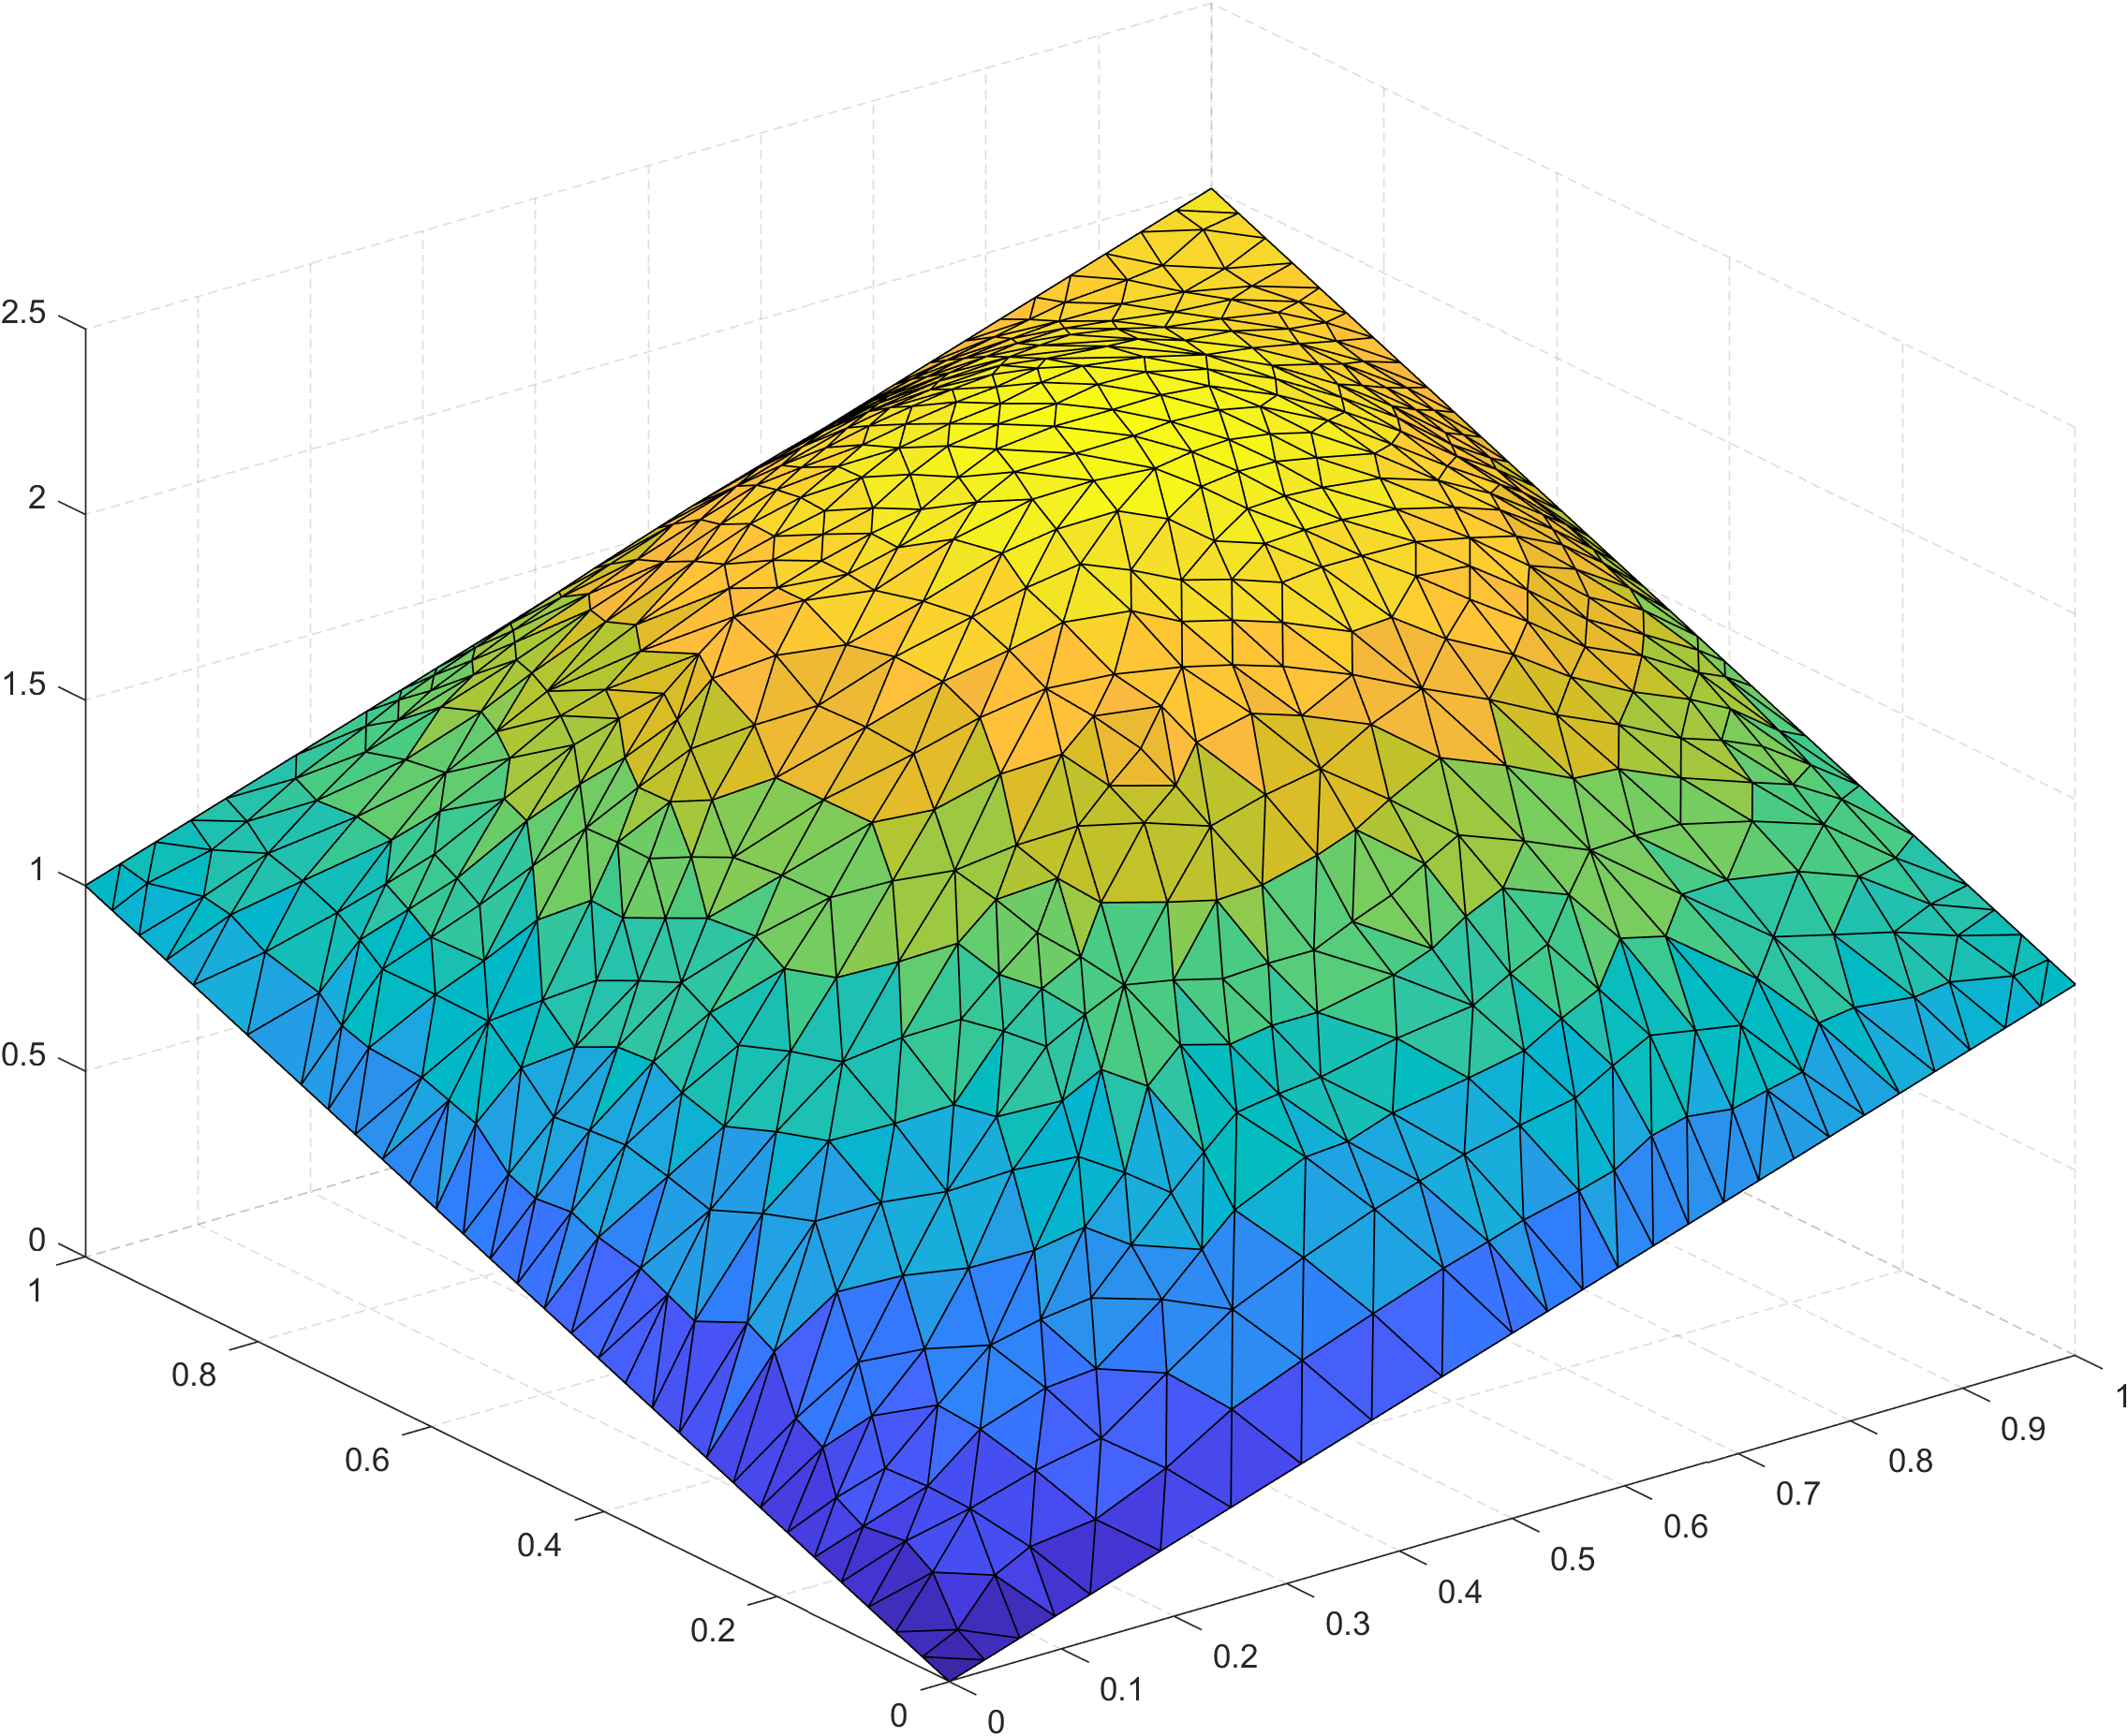
\includegraphics[height=\dimIm]{../Immagini/DNO_P2_AMax=0.005.png}
                        \caption{Soluzione qualitativa coi $\mathbb{P}_2.$}
                        \label{figDNOTriangolazioniApprossimataP2}
                    \end{subfigure}
                }
                \caption{Soluzioni del DNO: la prima è esatta e le altre due sono approssimate. I parametri dati a \textit{BBTR} sono spiegati nel $\S$\ref{parPremessaParametriBBTR}.}
                \label{figDNO}
            \end{figure*}
            
            {
            \setlength{\intextsep}{8pt}
            \begin{table}[H]
                \centering
                \newcommand{\sepCol}{\hspace{5pt}}
                \renewcommand{\arraystretch}{1.5}
                \begin{tabular}{c@{}|@{\sepCol}c@{\sepCol}c@{\sepCol}c@{\sepCol}c@{\sepCol}c}
                    $h$&
                    \notaSci{9.95}{-2}&
                    \notaSci{7.07}{-2}&
                    \notaSci{4.97}{-2}&
                    \notaSci{3.53}{-2}&
                    \notaSci{2.50}{-2}\\
                    \hline
                    $\text{err}_{L^2}^{\mathbb P_1}$&
                        \notaSci{1.65}{-2}&
                        \notaSci{7.58}{-3}&
                        \notaSci{3.85}{-3}&
                        \notaSci{1.95}{-3}&
                        \notaSci{9.32}{-4}\\
                    $\text{err}_{H^1}^{\mathbb P_1}$&
                        \notaSci{3.99}{-1}&
                        \notaSci{2.75}{-1}&
                        \notaSci{1.93}{-1}&
                        \notaSci{1.38}{-1}&
                        \notaSci{9.54}{-2}\\
                    $\text{err}_{L^2}^{\mathbb P_2}$&
                        \notaSci{3.34}{-4}&
                        \notaSci{1.38}{-4}&
                        \notaSci{4.58}{-5}&
                        \notaSci{1.60}{-5}&
                        \notaSci{5.56}{-6}\\
                    $\text{err}_{H^1}^{\mathbb P_2}$&
                        \notaSci{2.32}{-2}&
                        \notaSci{1.24}{-2}&
                        \notaSci{5.93}{-3}&
                        \notaSci{3.04}{-3}&
                        \notaSci{1.50}{-3}
                \end{tabular}
                \caption{Dati relativi all'errore nel DO.}
                \label{tabErroriDO}
            \end{table}
            }
            
            \begin{figure}[H]
                \centering 
                \newcommand{\lungSF}{.5\linewidth}
                \newcommand{\dimIm}{\linewidth}
                \makebox[\linewidth][c]{
                    \begin{subfigure}[t]{\lungSF}
                        \centering
                        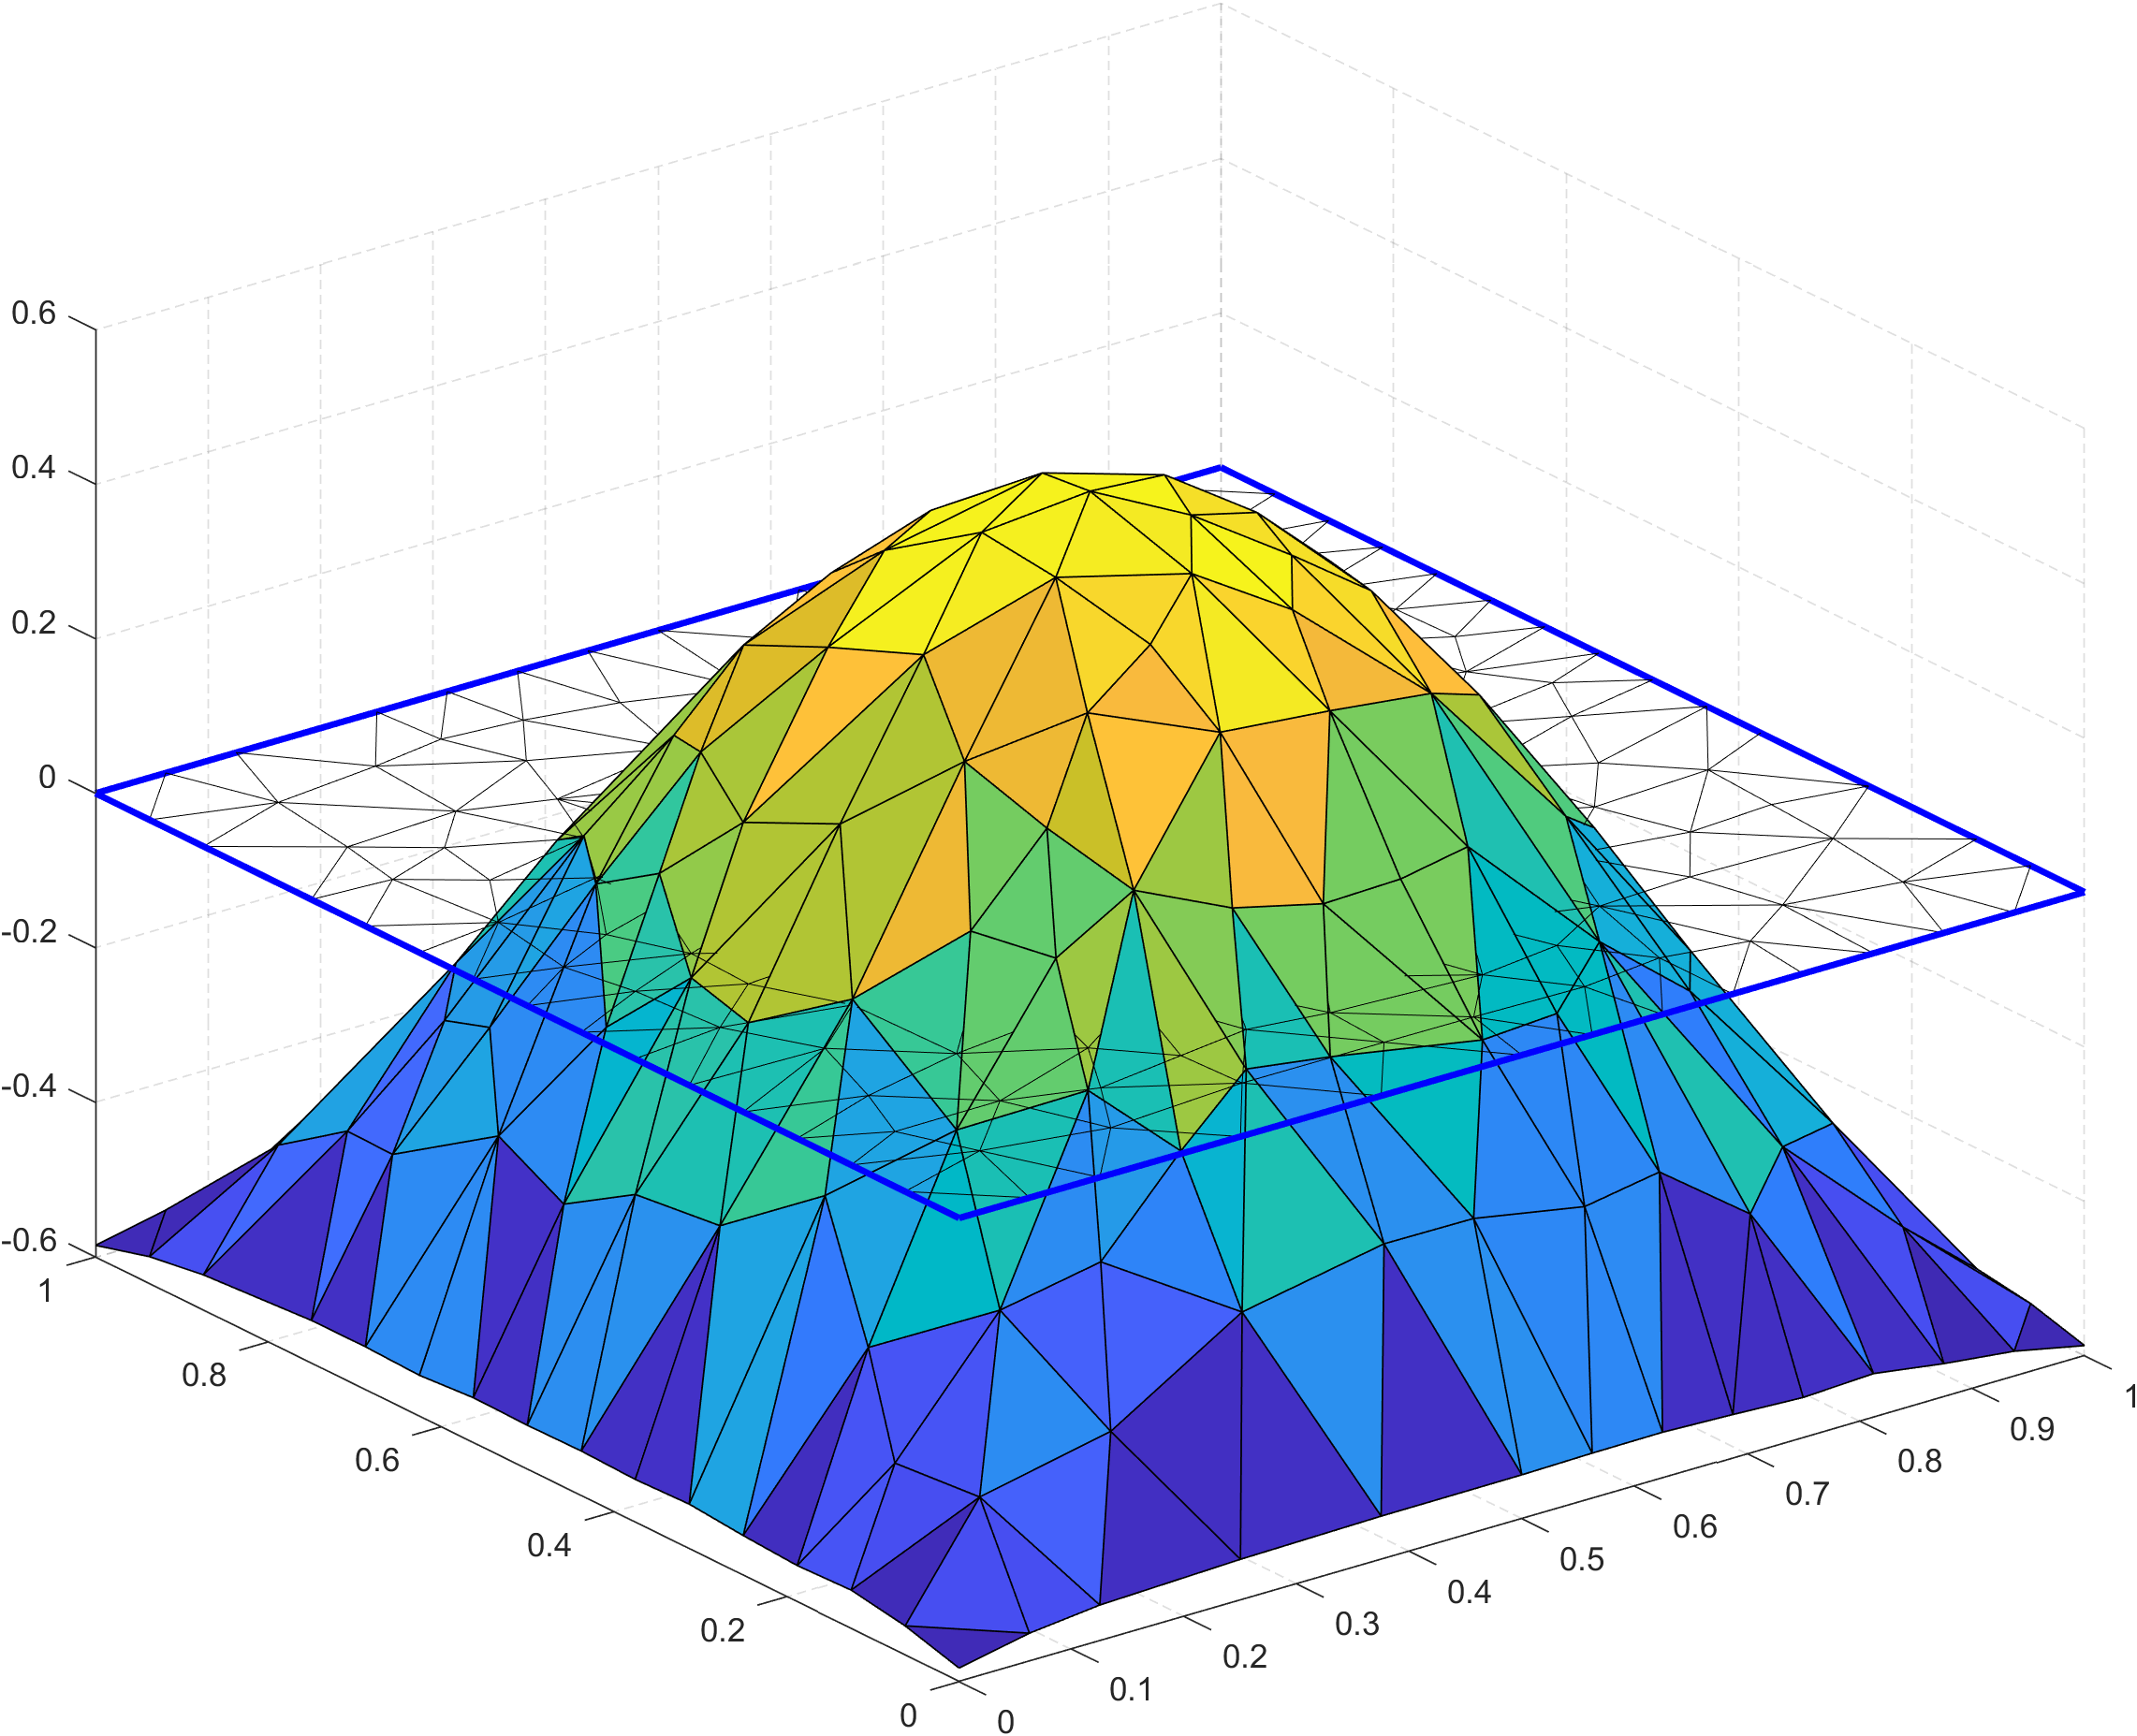
\includegraphics[width=\dimIm]{../Immagini/DO_P1_AMax=0.005_Tutto_Neumann.png}
                        \caption{Coi $\mathbb{P}_1$.}
                        \label{figDOEsplodenteP1}
                    \end{subfigure}
                    \begin{subfigure}[t]{\lungSF}
                        \centering
                        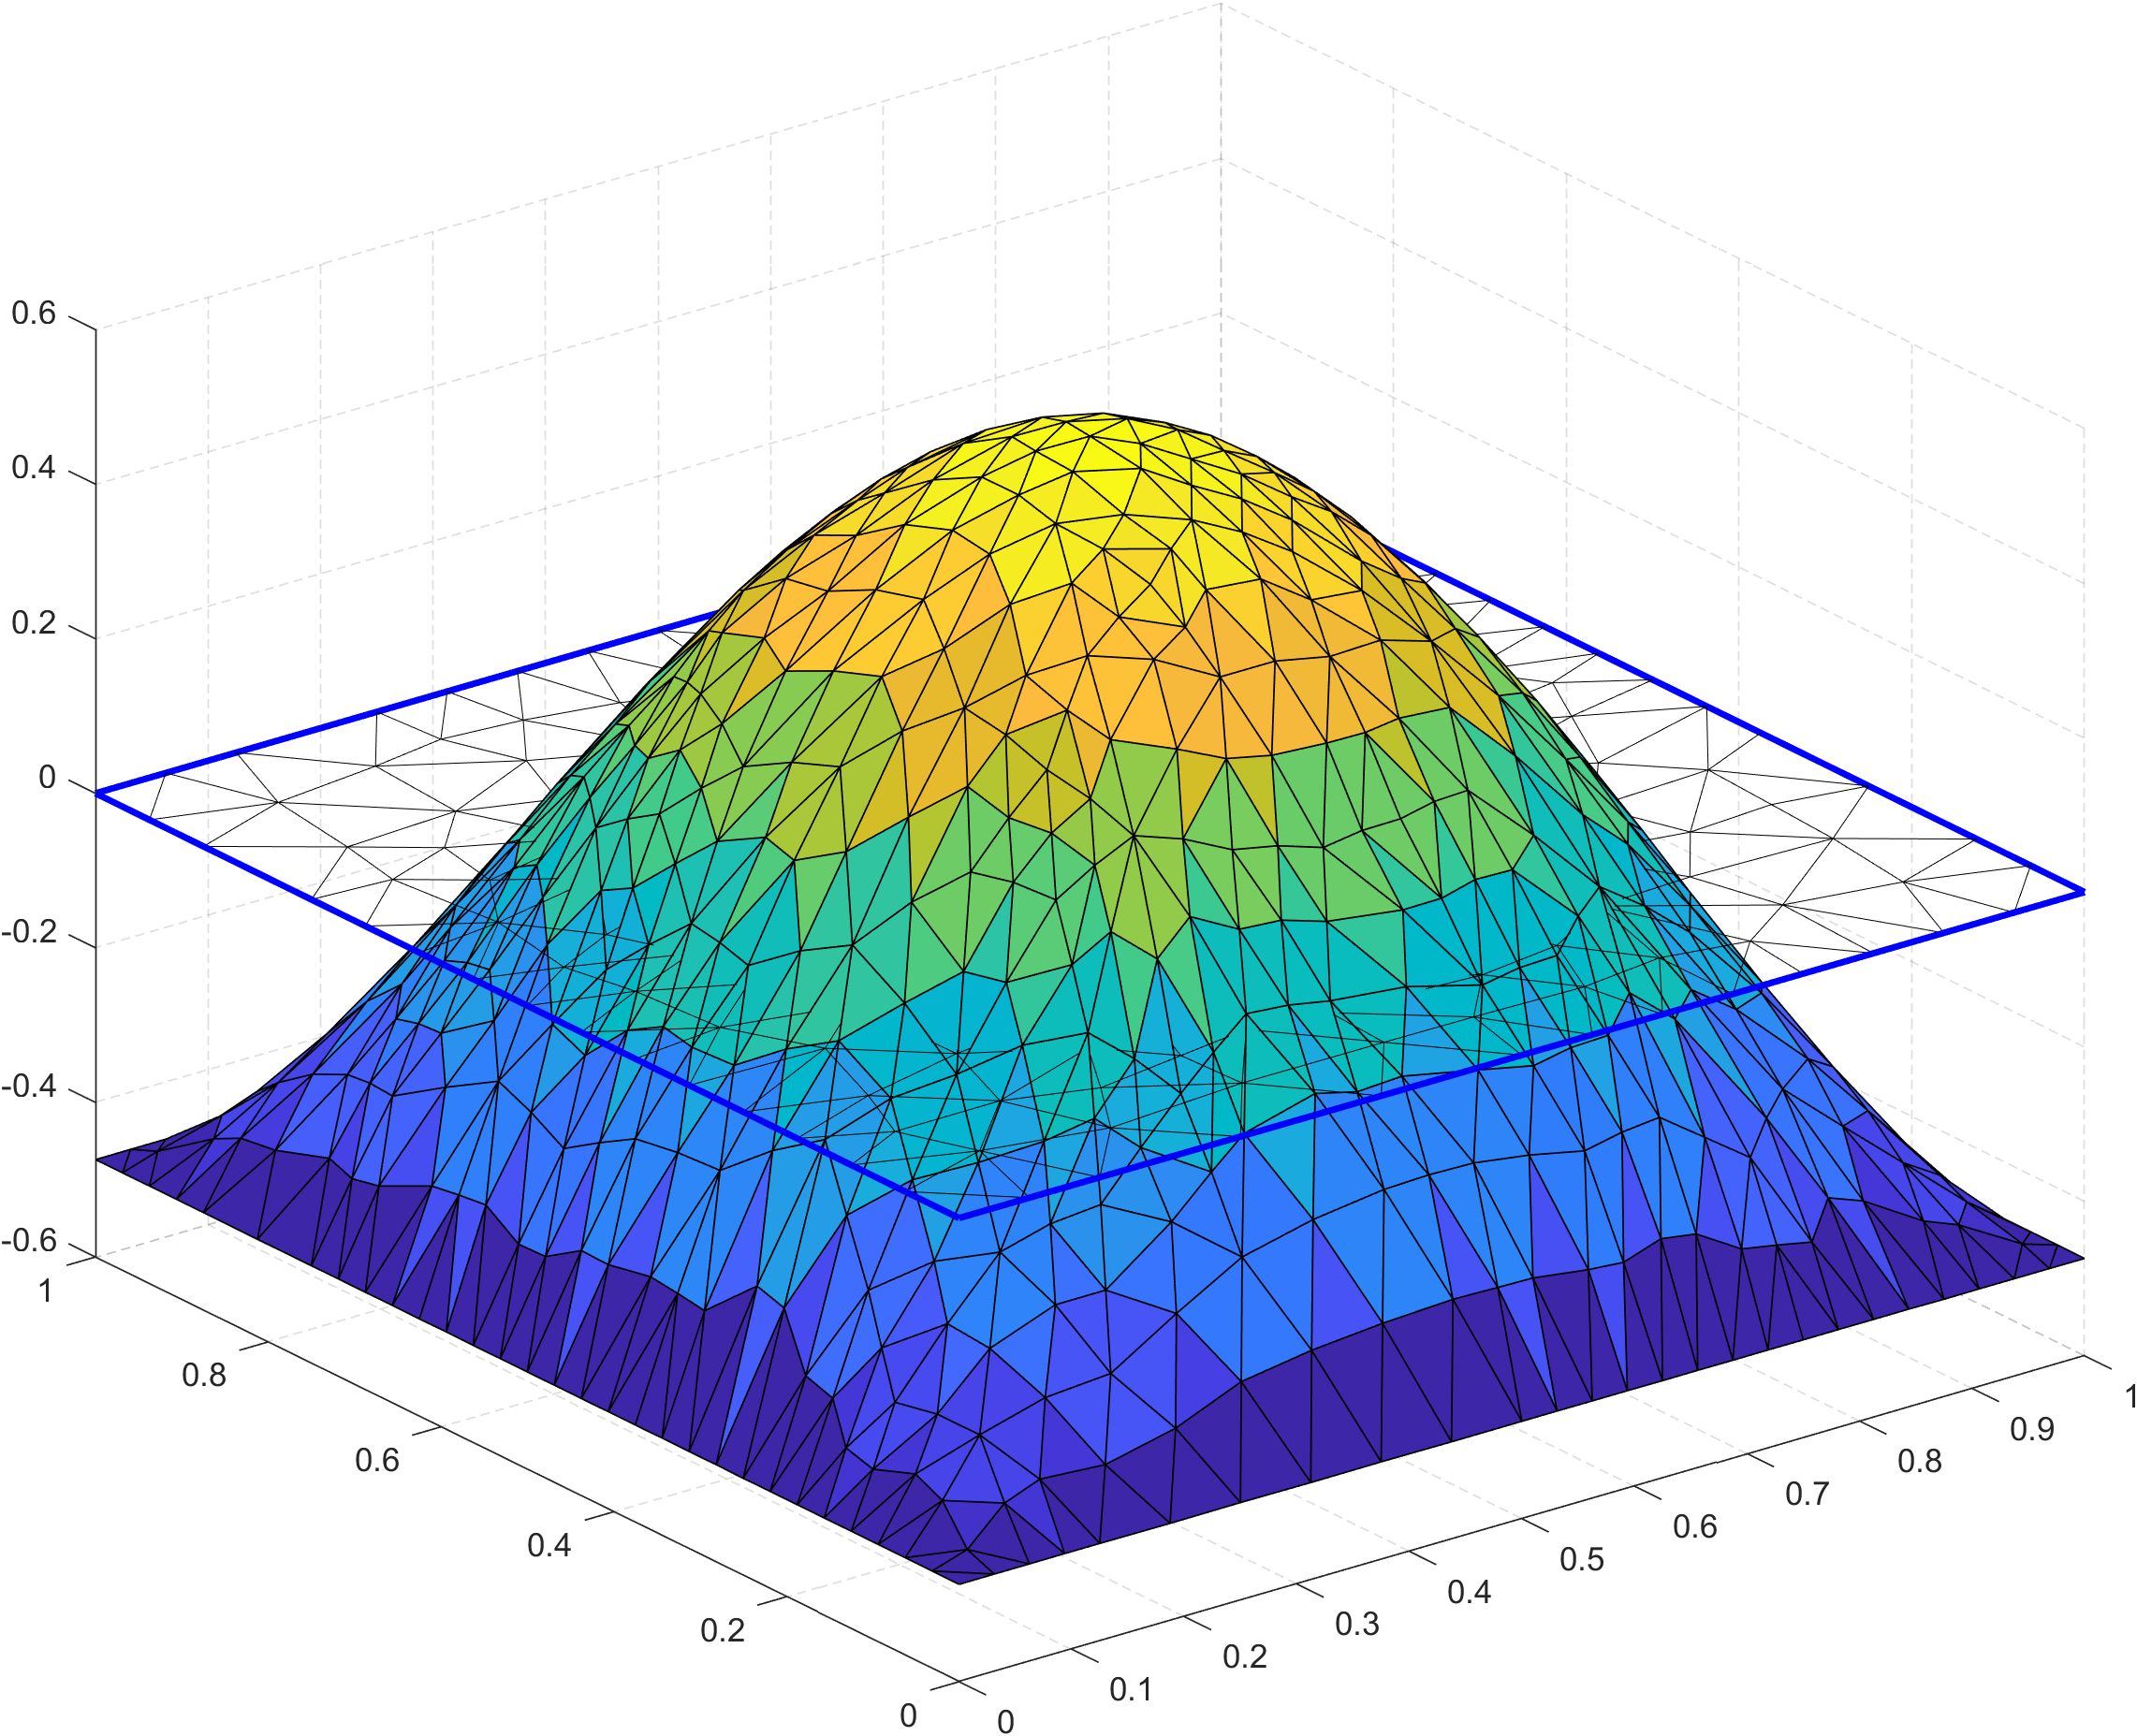
\includegraphics[width=\dimIm]{../Immagini/DO_P2_AMax=0.005_Tutto_Neumann.png}
                        \caption{Coi $\mathbb{P}_2$.}
                        \label{figDOEsplodenteP2}
                    \end{subfigure}
                }
                \caption{Soluzioni qualitative del DO con $\Gamma_N=\partial\Omega$.}
            \end{figure}


        \subsection{Dirichlet non omogeneo (DNO)}

            Esso consiste in un problema del tutto analogo al \eqref{eqDO} ma con condizione al bordo di Dirichlet non omogenea
            %
            \begin{equation*}
                g_D=x+y,
            \end{equation*}
            %
            che equivale a trasformare il \teqref{eqProblemaStazionario}{[PS]} in
            %
            \begin{equation*}
                \left\{
                \begin{aligned}
                    -\Delta u&=f&\text{in }&\Omega, \\
                            u&=x+y&\text{su }&\partial\Omega,
                \end{aligned}
                \right.
                \label{eqDNO}
            \end{equation*}
            %
            ove s'impone che la soluzione esatta $u$ sia pari a
            %
            \begin{equation}
                u=16x(1-x)y(1-y)+x+y.
                \label{eqSoluzioneEsattaDNO}
            \end{equation}
            %
            Nella Fig. \ref{figDNOTriangolazioniEsatta} è mostrata la soluzione esatta mentre nelle Figg. \ref{figDNOTriangolazioniApprossimataP1} e \ref{figDNOTriangolazioniApprossimataP2} le due approssimate mediante i $\mathbb P_1$ e i $\mathbb P_2$ rispettivamente.

            Curiosamente abbiamo riscontrato che gli errori commessi sono fondamentalmente identici a quelli del DO, mostrati nella Tab. \ref{tabErroriDO}, e dunque i grafici degli errori sono uguali alle Figg. \ref{figDOErroreP1Lin}-\ref{figDOErroreP2Log}.
            
            Come nel DO, anche qui il bordo \textit{non} può essere solo di Neumann per le medesime motivazioni, altrimenti la soluzione si comporta analogamente a prima come mostrano le Figg. \ref{figDNOEsplodenteP1} e \ref{figDNOEsplodenteP2}.

            \begin{figure}[H]
                \centering 
                \newcommand{\lungSF}{.5\linewidth}
                \newcommand{\dimIm}{\linewidth}
                \makebox[\linewidth][c]{
                    \begin{subfigure}[t]{\lungSF}
                        \centering
                        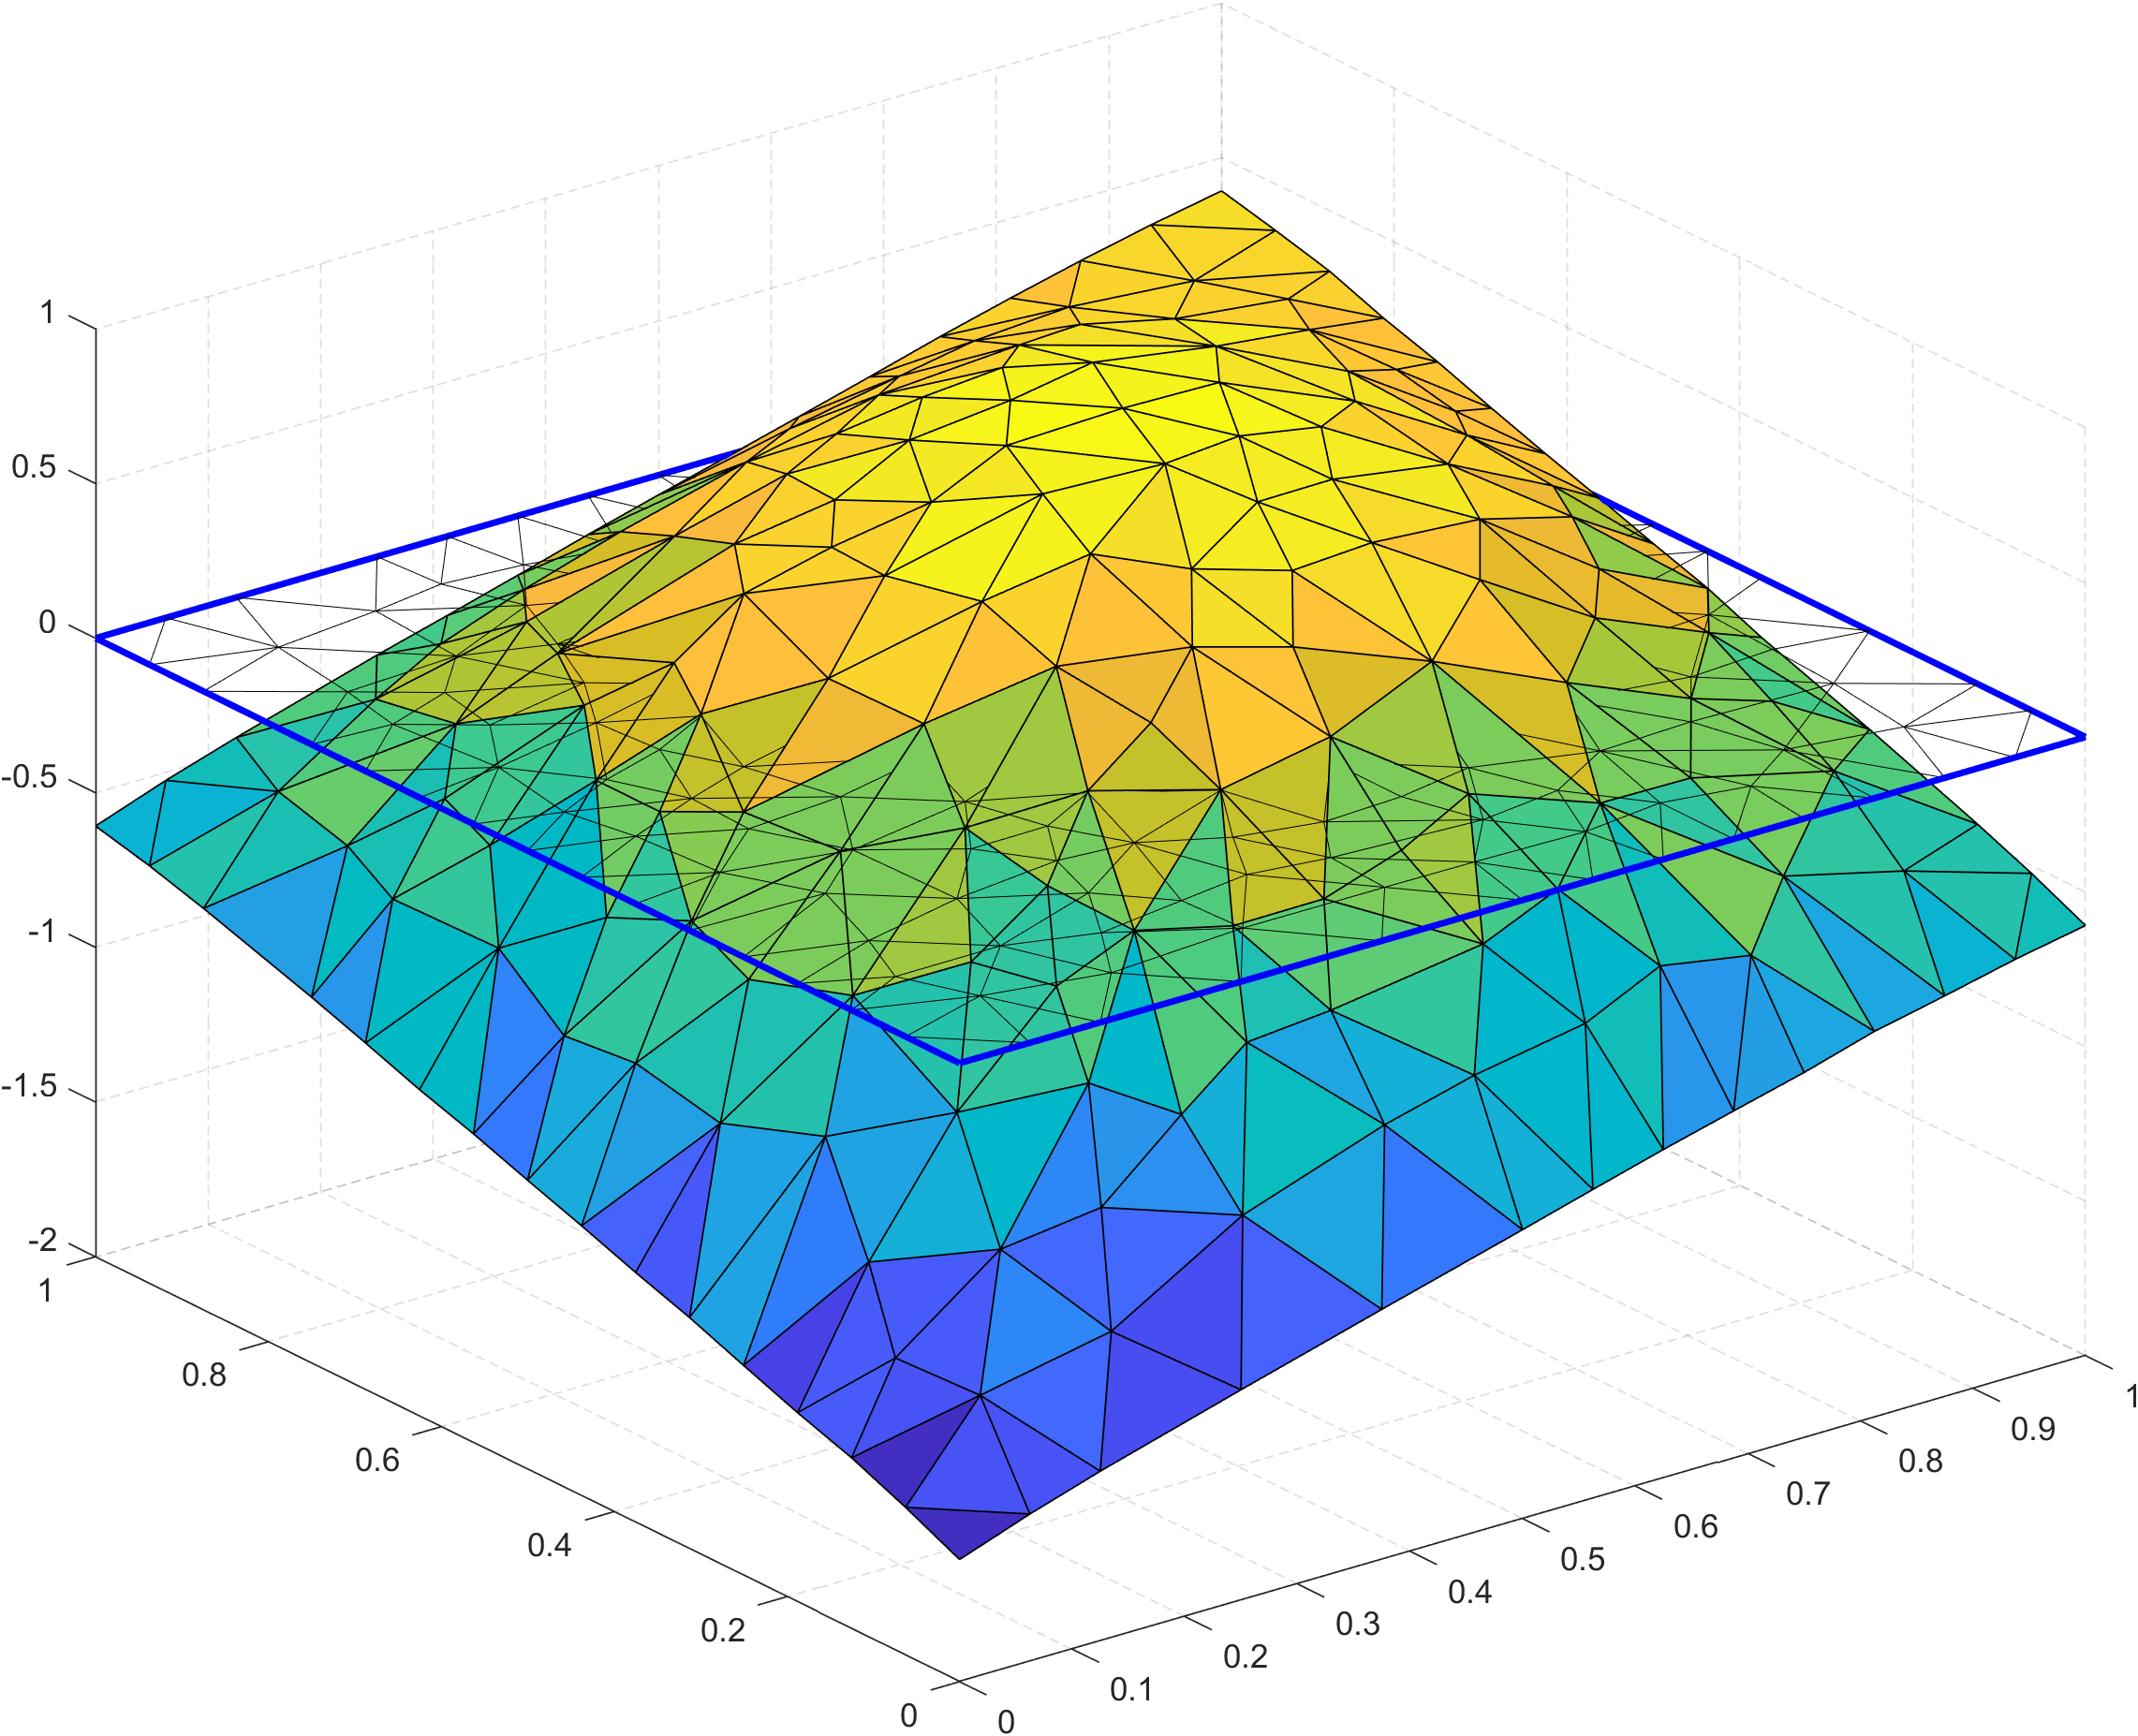
\includegraphics[width=\dimIm]{../Immagini/DNO_P1_AMax=0.005_Tutto_Neumann.png}
                        \caption{Coi $\mathbb{P}_1$.}
                        \label{figDNOEsplodenteP1}
                    \end{subfigure}
                    \begin{subfigure}[t]{\lungSF}
                        \centering
                        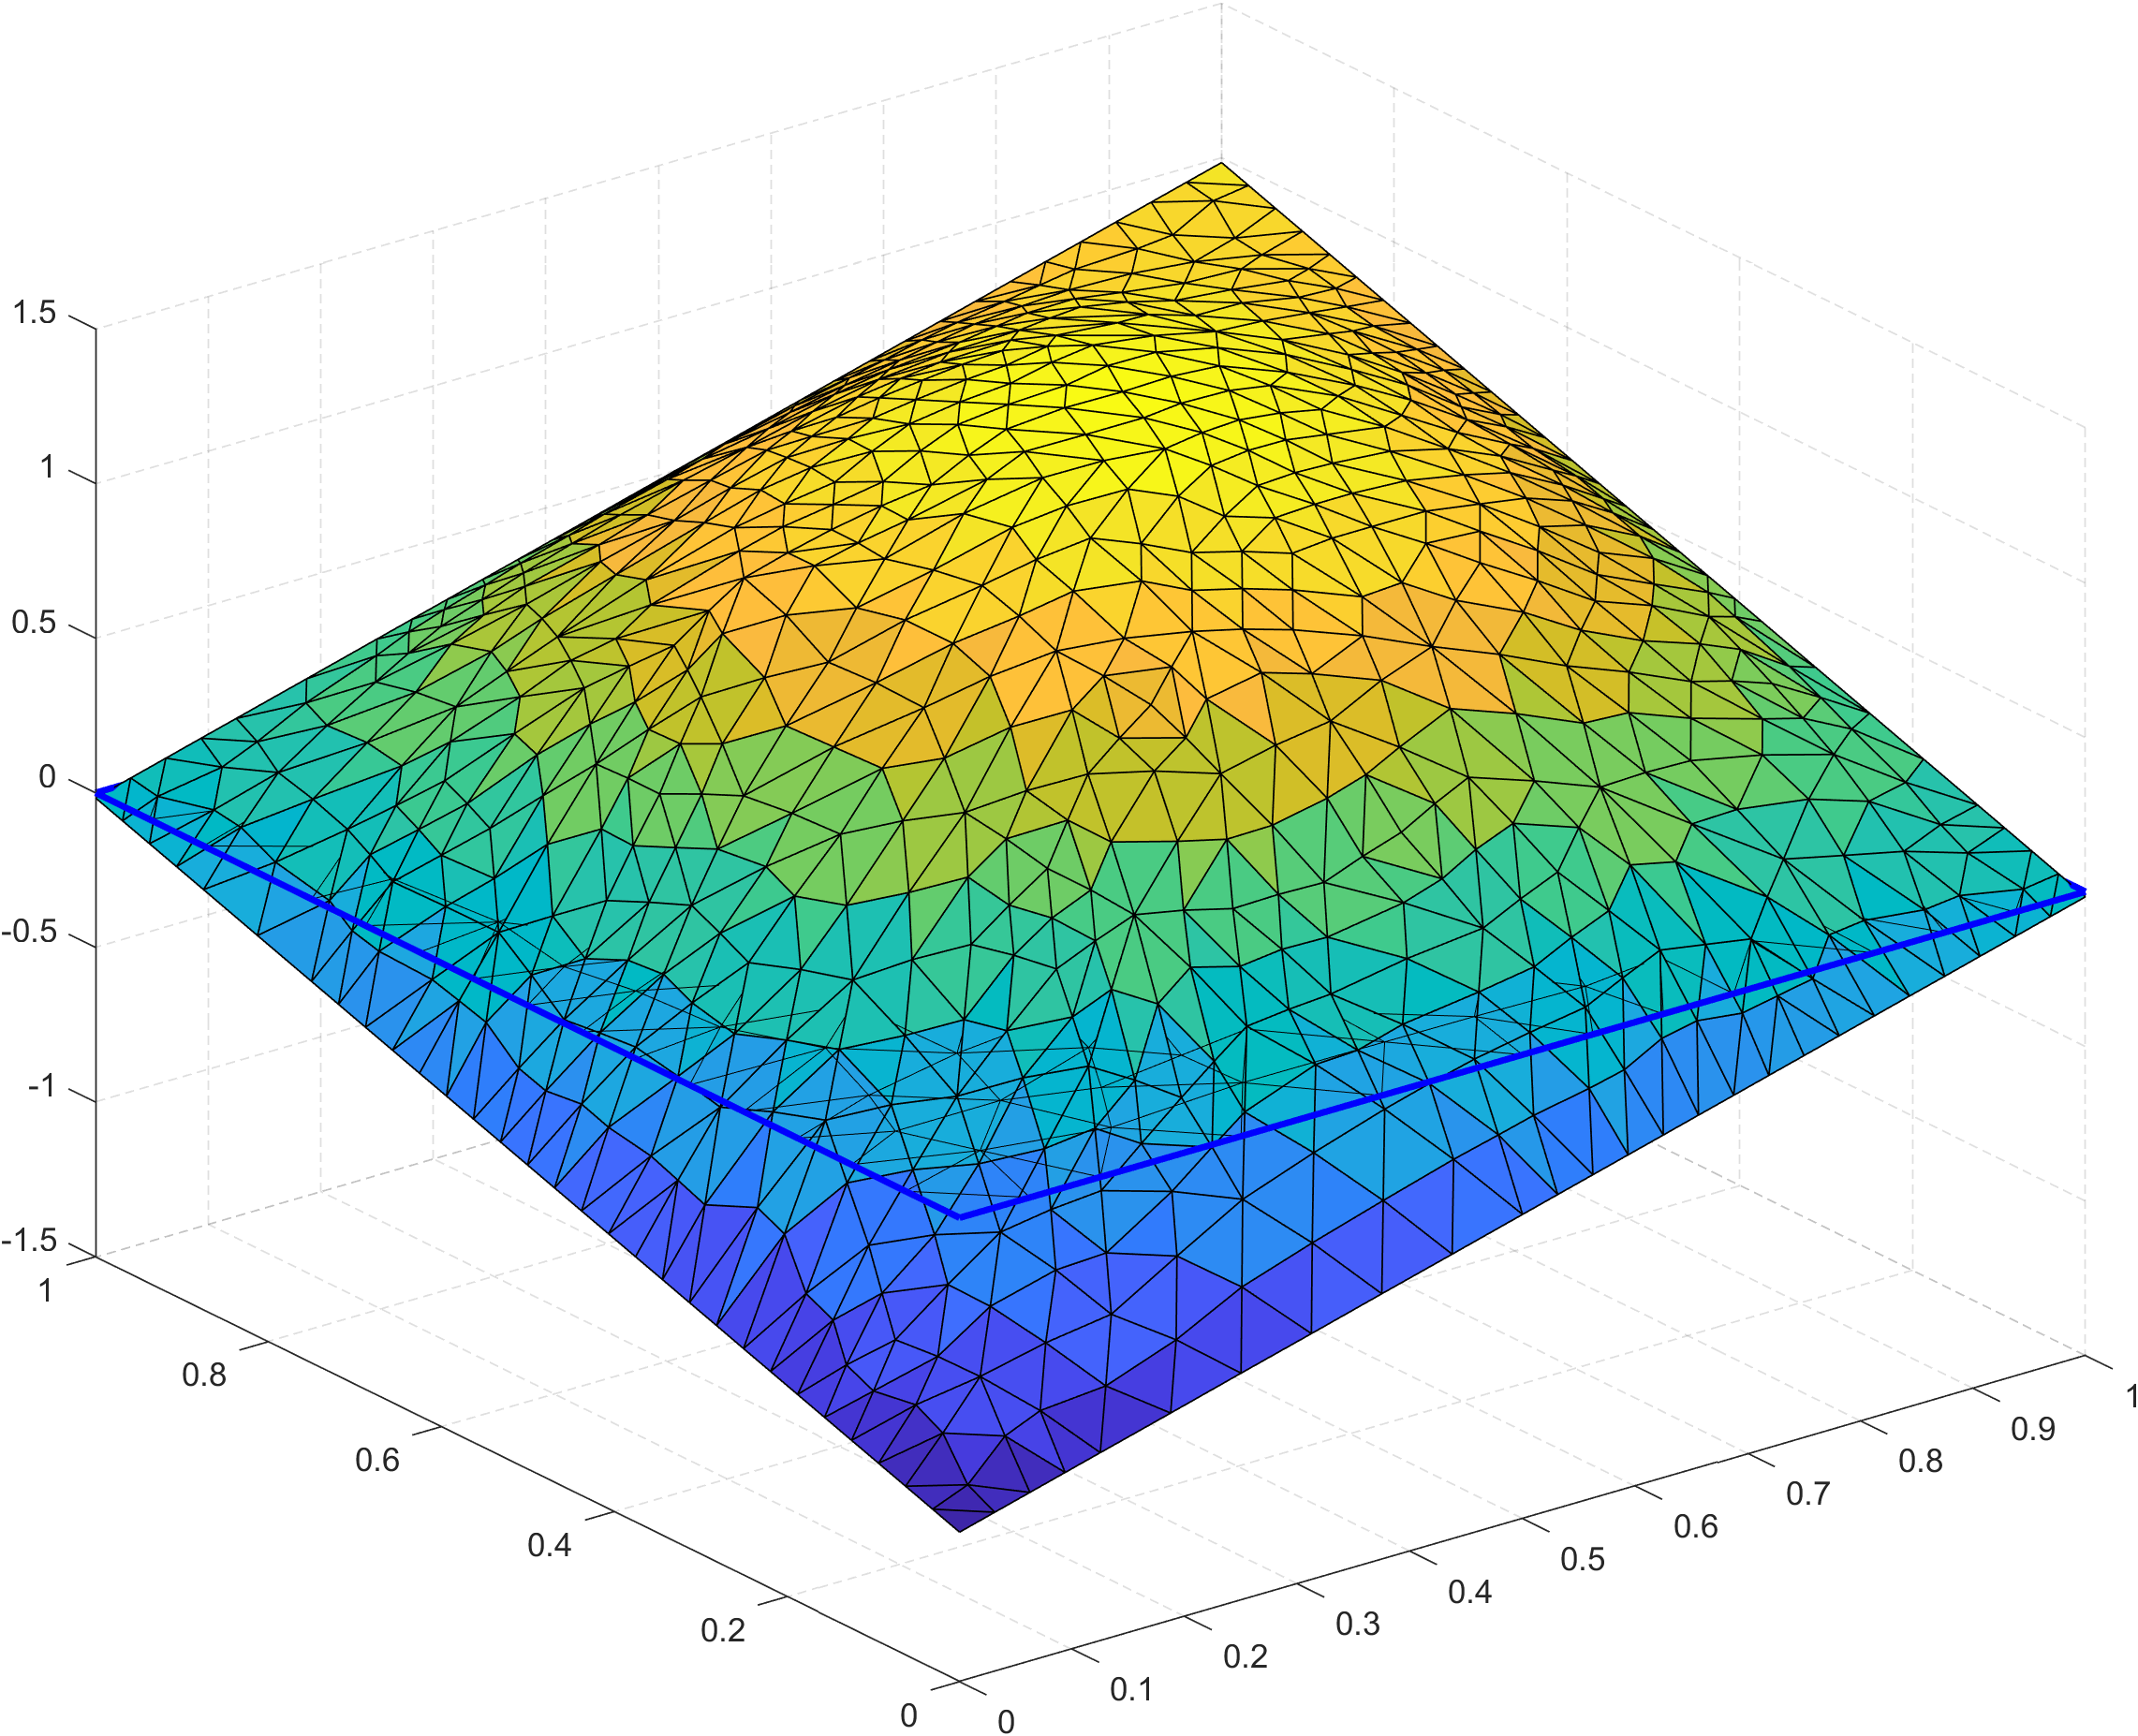
\includegraphics[width=\dimIm]{../Immagini/DNO_P2_AMax=0.005_Tutto_Neumann.png}
                        \caption{Coi $\mathbb{P}_2$.}
                        \label{figDNOEsplodenteP2}
                    \end{subfigure}
                }
                \caption{Soluzioni qualitative del DNO con $\Gamma_N=\partial\Omega$.}
            \end{figure}


        \subsection{Stabilità diffusione-convezione (SDC)}

            \subsubsection{Impostazione e instabilità}\label{parInstabilitàSDC}
                
                Esso consiste in un problema di diffusione debole e di convezione con velocità $\boldsymbol\beta$ lungo l'ascissa e di norma unitaria, ovvero
                %
                \begin{equation*}
                    \setlength{\abovedisplayskip}{5pt plus 2pt minus 2pt}  % Riduce lo spazio sopra l'equazione
                    \setlength{\belowdisplayskip}{5pt plus 2pt minus 2pt}  % Riduce lo spazio sotto l'equazione
                    \SpaziaturaMate{1}{2}{3}
                    \nu=10^{-6},\;\;\beta=(1,0)^{\top}\text{ e }\sigma=0;
                \end{equation*}
                %
                ciò equivale a trasformare il \teqref{eqProblemaStazionario}{[PS]} in
                %
                \begin{equation}
                    \left\{
                    \begin{aligned}
                        -10^{-6}\Delta u+\derP ux&=f&\text{in }&\Omega, \\
                        u&=u\vert_{\partial\Omega}&\text{su }&\partial\Omega.
                    \end{aligned}
                    \right.
                    \label{eqSDC}
                \end{equation}
                %
                Per quanto riguarda la soluzione esatta $u$ s'impone in un primo momento che sia pari a
                %
                \begin{equation}
                    u=16x(1-x)y(1-y)e^{4x}+x+y,
                    \label{eqSoluzioneEsattaSDC1}
                \end{equation}
                %
                che equivale a moltiplicare la parte omogenea della \eqref{eqSoluzioneEsattaDNO} per $e^{4x}$: questo rende la soluzione molto ripida vicino al bordo destro del dominio quadrato. Invece in un secondo momento s'impone che la soluzione esatta sia uguale a
                %
                \begin{equation}
                    u=A\exp\left(-\frac\alpha
                    {\left(\frac{x(1-x)}{1+\varepsilon}+\varepsilon\right)
                    \left(\frac{y(1-y)}{1+\varepsilon}+\varepsilon\right)}\right),
                    \label{eqSoluzioneEsattaSDC2}
                \end{equation}
                %
                ove $A=\exp(\alpha/(0.5^2/(1+\varepsilon)+\varepsilon)^2)$, $\alpha=0.005$ ed $\varepsilon=0.0005$ (la $\varepsilon$ serve solo a garantire che la derivata della \eqref{eqSoluzioneEsattaSDC2} non esploda ai bordi); questa risulta una funzione piú ``cattiva'' nel senso che decade molto rapidamente su tutt'i bordi del dominio. Queste due soluzioni saranno indicati cogli acronimi SDC1 ed SDC2 rispettivamente.

                Perdipiú, dai valori delle costanti nel \eqref{eqSDC}, è chiaro che il problema in esame sia a convezione dominante come mostra il numero di Péclet locale
                %
                \begin{equation}
                    Pe_T=m_k\frac{\Vert\beta\Vert_Th_T}{2\nu}=m_kh_T5\times10^5\gg1,
                    \label{eqNumeroPeclet}
                \end{equation}
                %
                in cui $\Vert\beta\Vert_T\equiv\Vert\beta\Vert_2$, $m_1=1/3$, $m_2=1/24$ mentre $h_T$ è il diametro dell'EF, ossia il suo piú lungo lato. E siccome il prodotto $m_kh_T$ non è in grado di portare il numero di Péclet al di sotto dell'unità, anche per bassi valori di $h_T$, dalla teoria (si v. \cite{dispenseMEDèPA} $\S11.1$ per maggiori dettagli) si ha che la soluzione è instabile, come mostrano le Figg. \ref{figSDC1InstabileP1},\ref{figSDC1InstabileP2} per la \eqref{eqSoluzioneEsattaSDC1}, e le Figg. \ref{figSDC2InstabileP1},\ref{figSDC2InstabileP2} per la \eqref{eqSoluzioneEsattaSDC2}.

                {\SpaziaturaMate{1}{2}{3}
                Si osservi come la medesima instabilità si può manifestare anche con viscosità $\nu\approx1$ ma velocità convettiva $\Vert\boldsymbol\beta\Vert_2\gg1$: l'importante è che la distanza tra i due coefficienti sia elevata\footnote{Quei valori sono frequenti ad esempio in fluidodinamica ove le velocità posso assumere valori oltre il numero di Mach, mentre la viscosità rimane costante [uguale a quella dell'aria o dell'acqua]; infatti in tali contesti le instabilità del MEF portano a preferire altri metodi come quello dei volumi finiti.}.}
                
                {\setlength{\intextsep}{0pt}
                \begin{figure}[H]
                    \centering 
                    \newcommand{\lungSF}{.5\linewidth}
                    \newcommand{\dimIm}{\linewidth}
                    \makebox[\linewidth][c]{
                        \begin{subfigure}[t]{\lungSF}
                            \centering
                            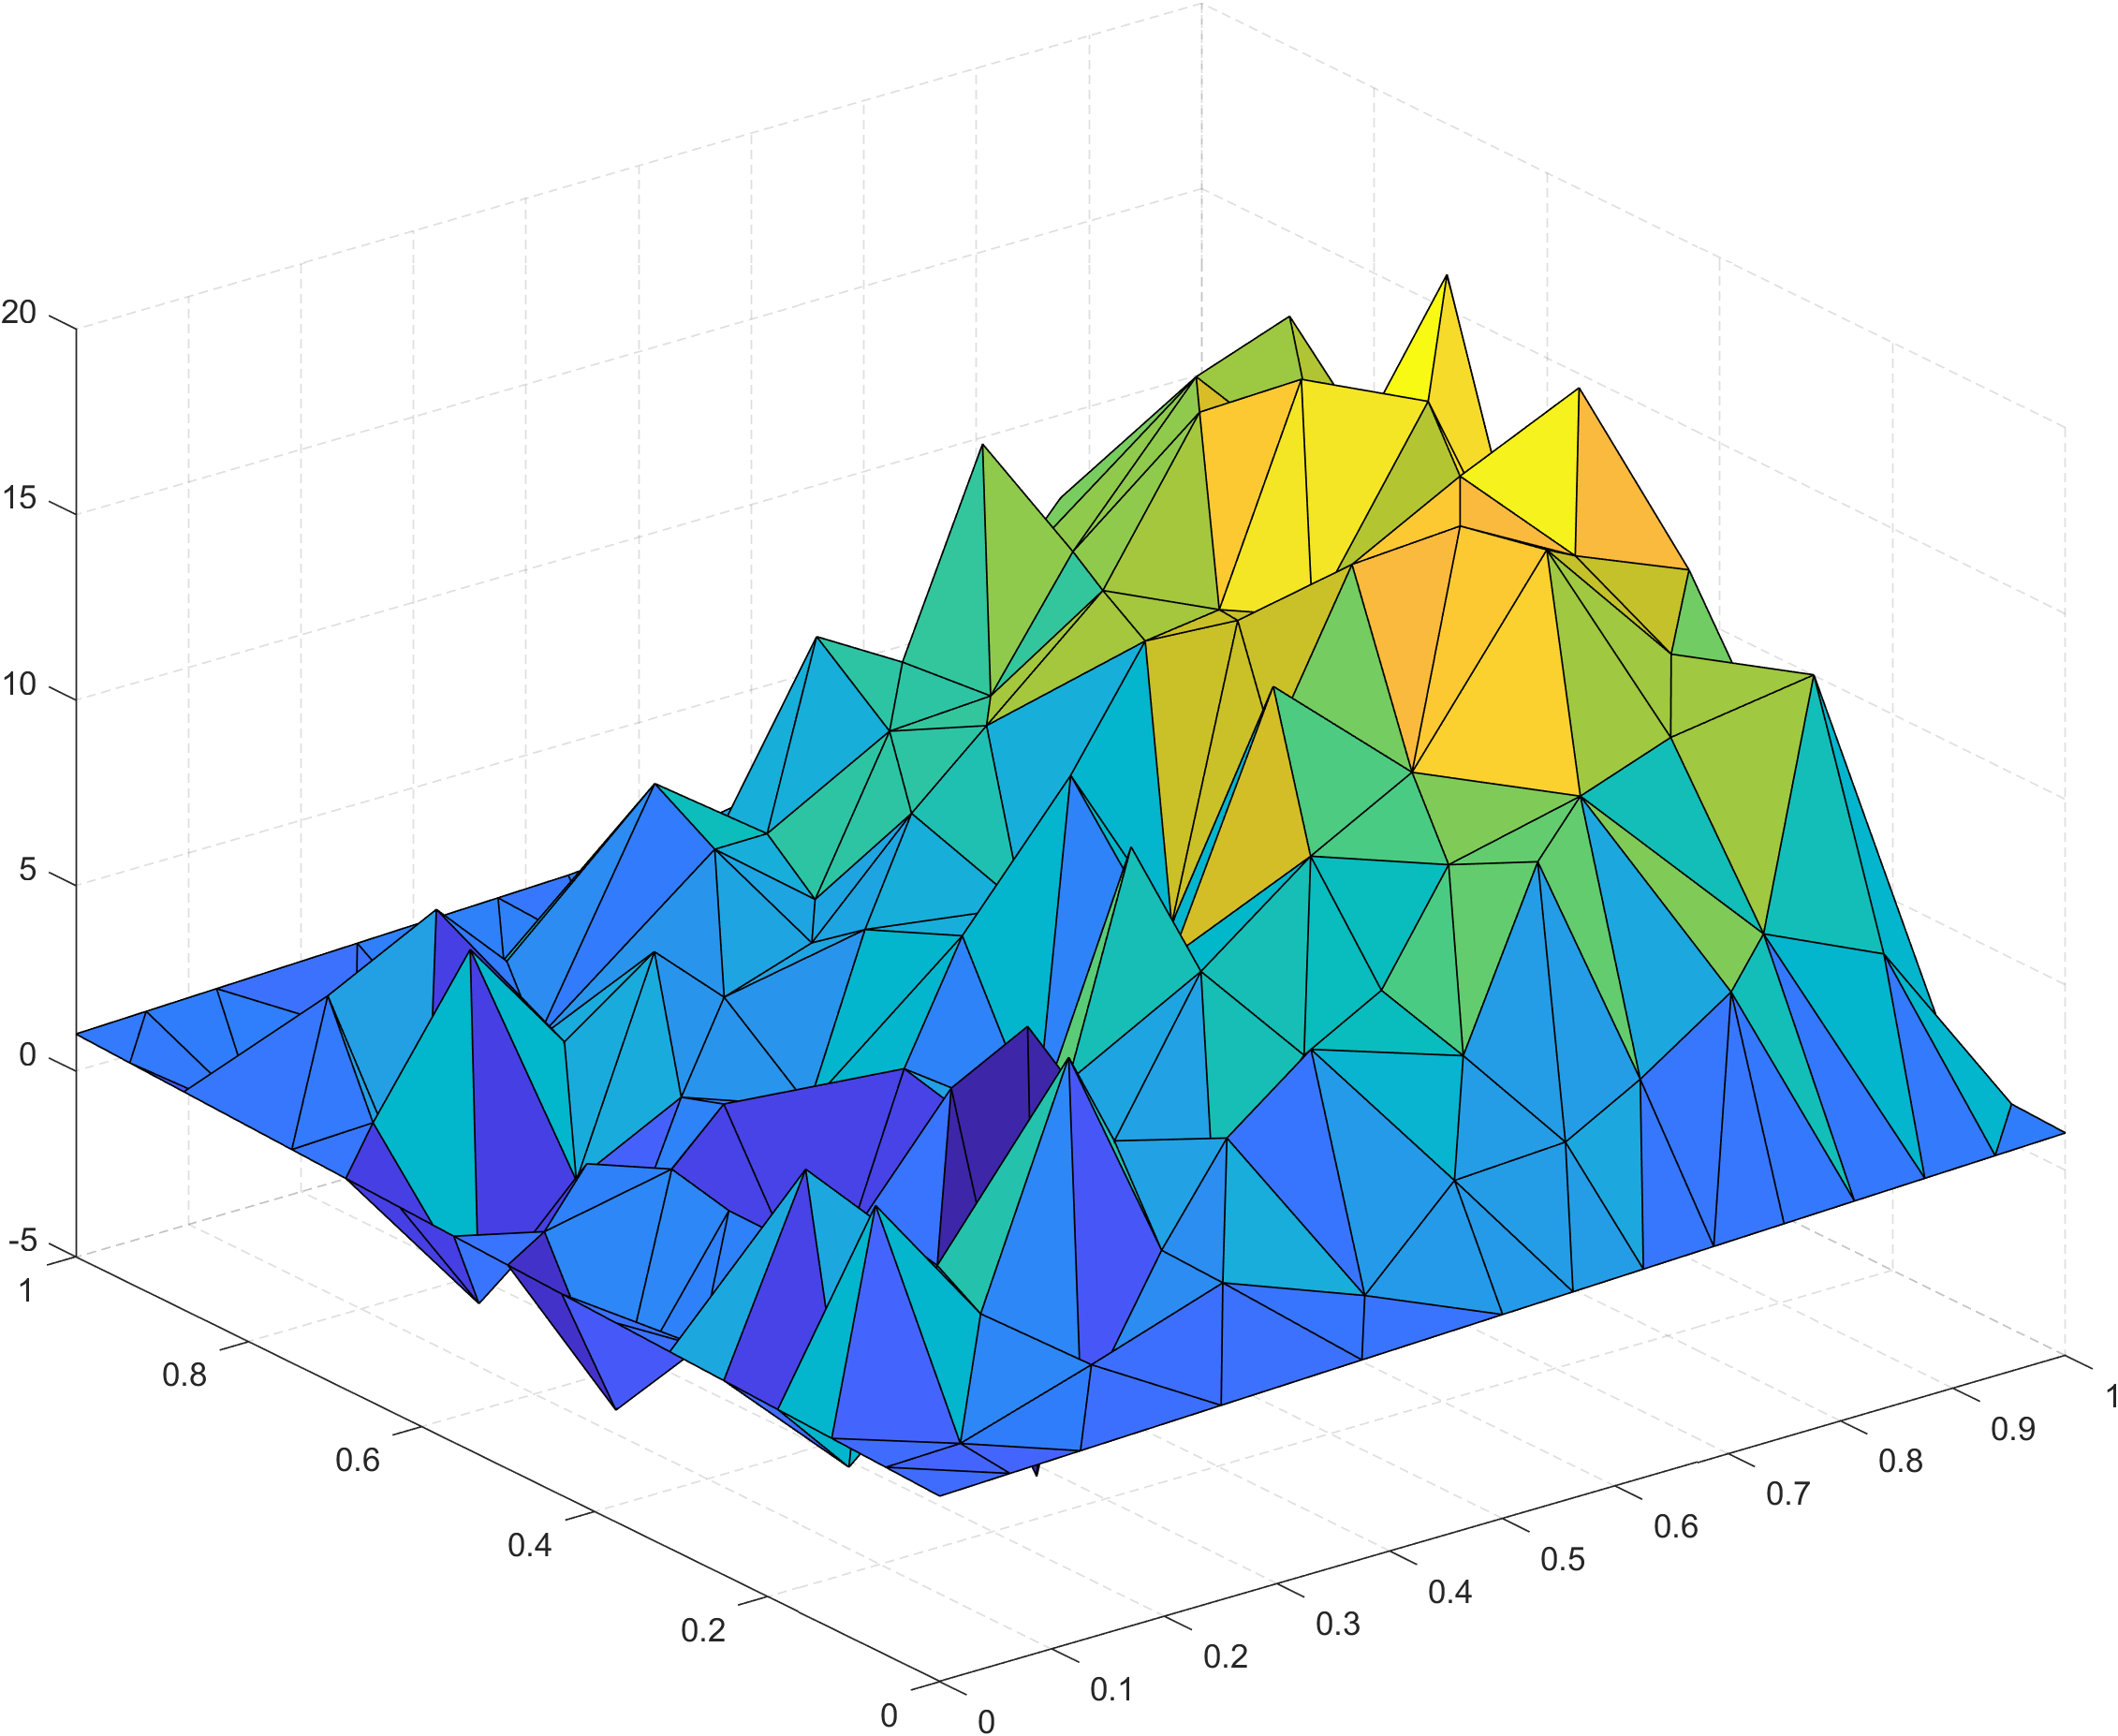
\includegraphics[width=\dimIm]{../Immagini/SDC1_SS_P1_AMax=0.005.png}
                            \caption{Coi $\mathbb{P}_1$.}
                            \label{figSDC1InstabileP1}
                        \end{subfigure}
                        \begin{subfigure}[t]{\lungSF}
                            \centering
                            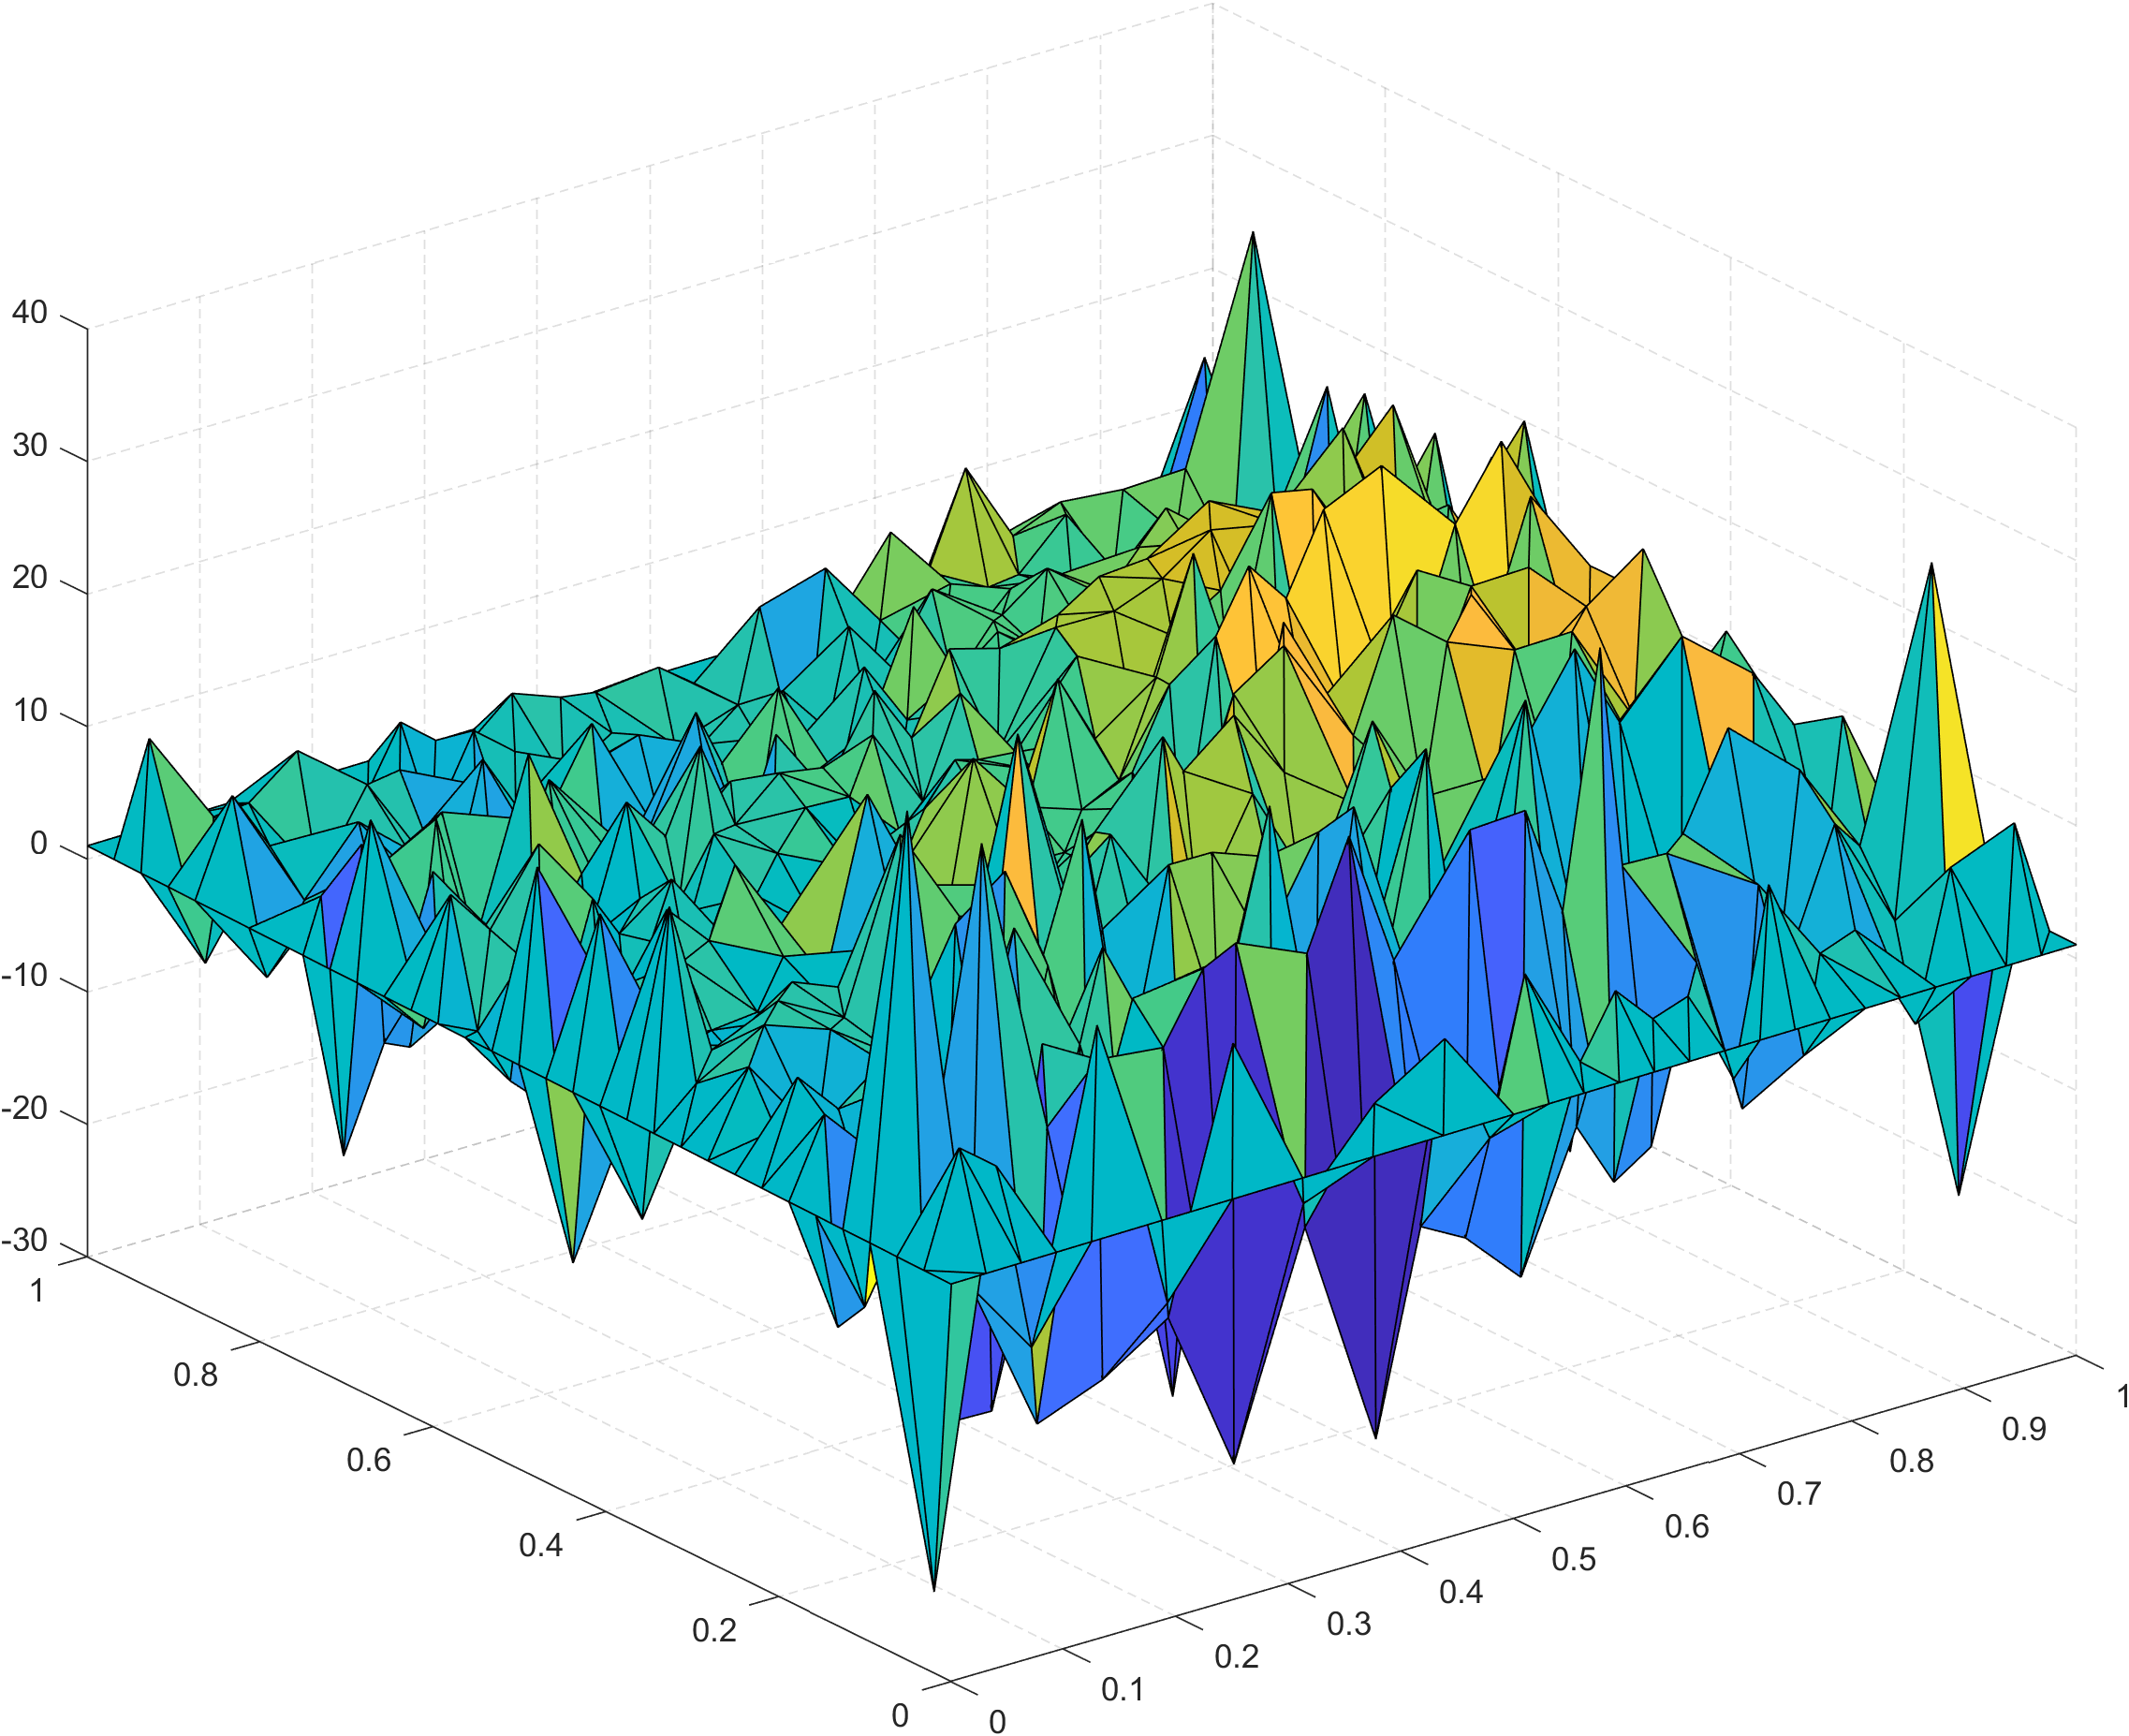
\includegraphics[width=\dimIm]{../Immagini/SDC1_SS_P2_AMax=0.005.png}
                            \caption{Coi $\mathbb{P}_2$.}
                            \label{figSDC1InstabileP2}
                        \end{subfigure}
                    }
                    \caption{Soluzione qualitativa dell'SDC1 instabile.}
                \label{figSDC1Instabile}
                \end{figure}
                \begin{figure}[H]
                    \centering 
                    \newcommand{\lungSF}{.5\linewidth}
                    \newcommand{\dimIm}{\linewidth}
                    \makebox[\linewidth][c]{
                        \begin{subfigure}[t]{\lungSF}
                            \centering
                            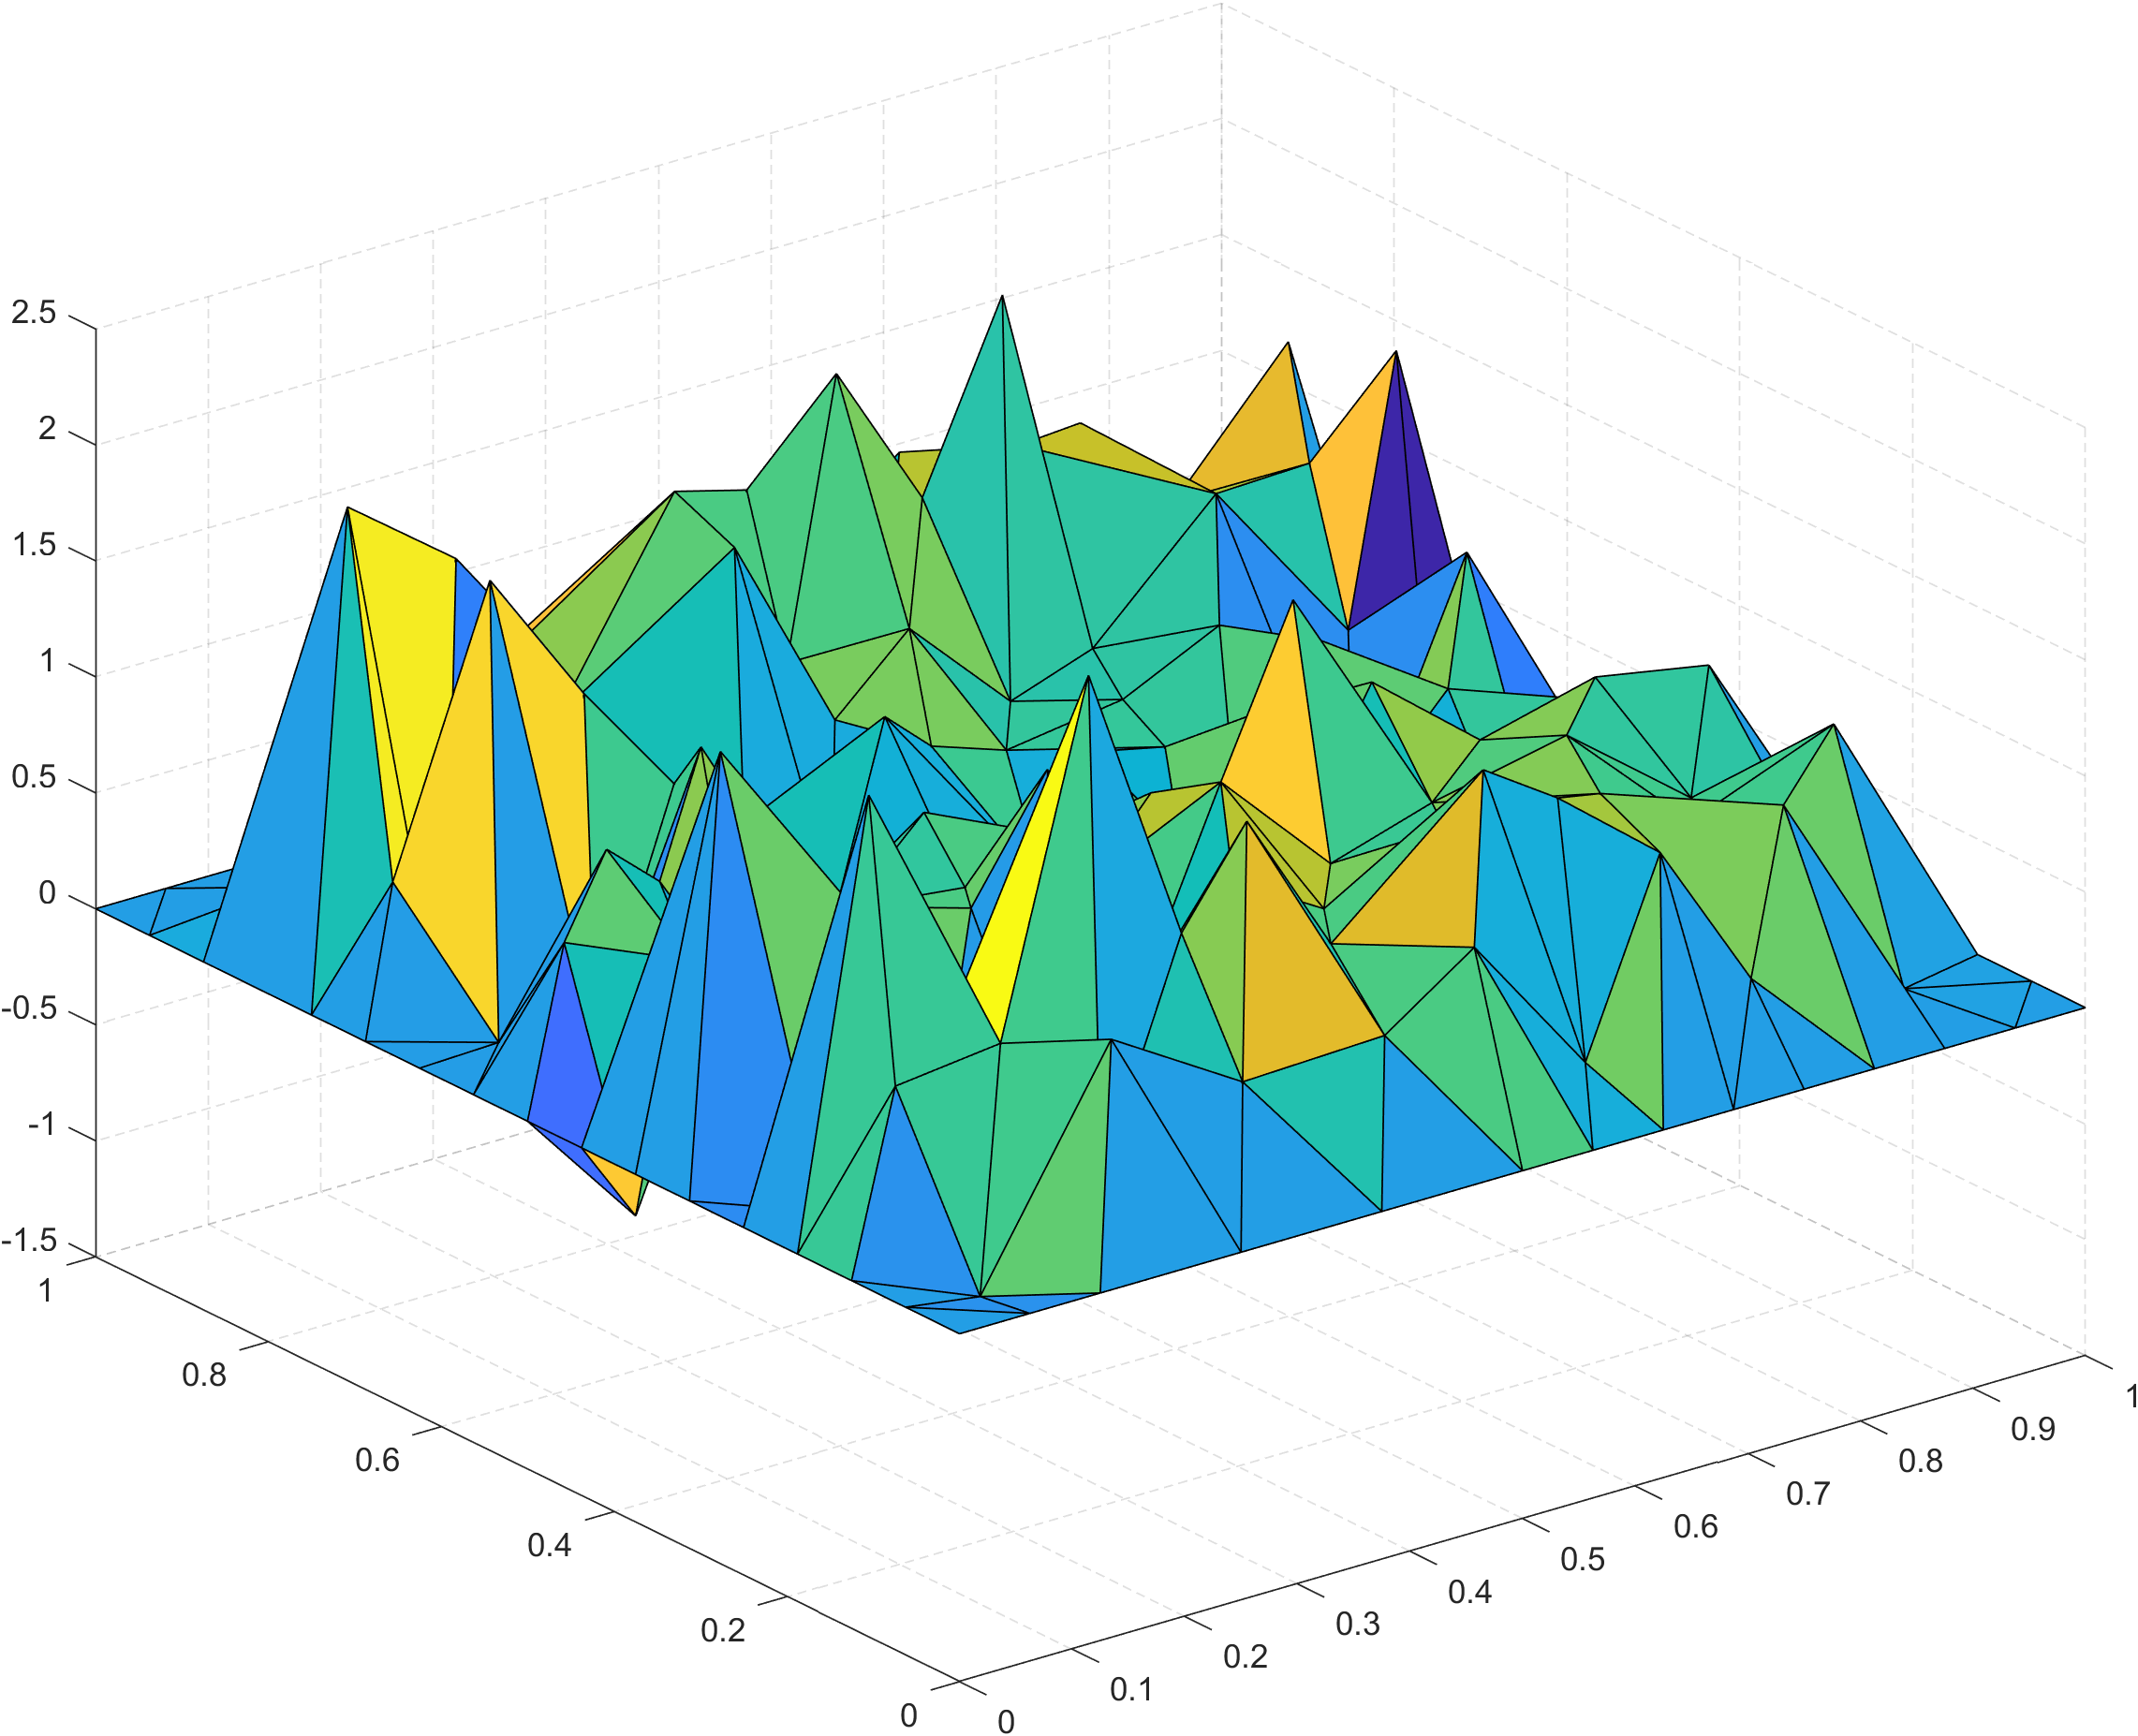
\includegraphics[width=\dimIm]{../Immagini/SDC2_SS_P1_AMax=0.005.png}
                            \caption{Coi $\mathbb{P}_1$.}
                            \label{figSDC2InstabileP1}
                        \end{subfigure}
                        \begin{subfigure}[t]{\lungSF}
                            \centering
                            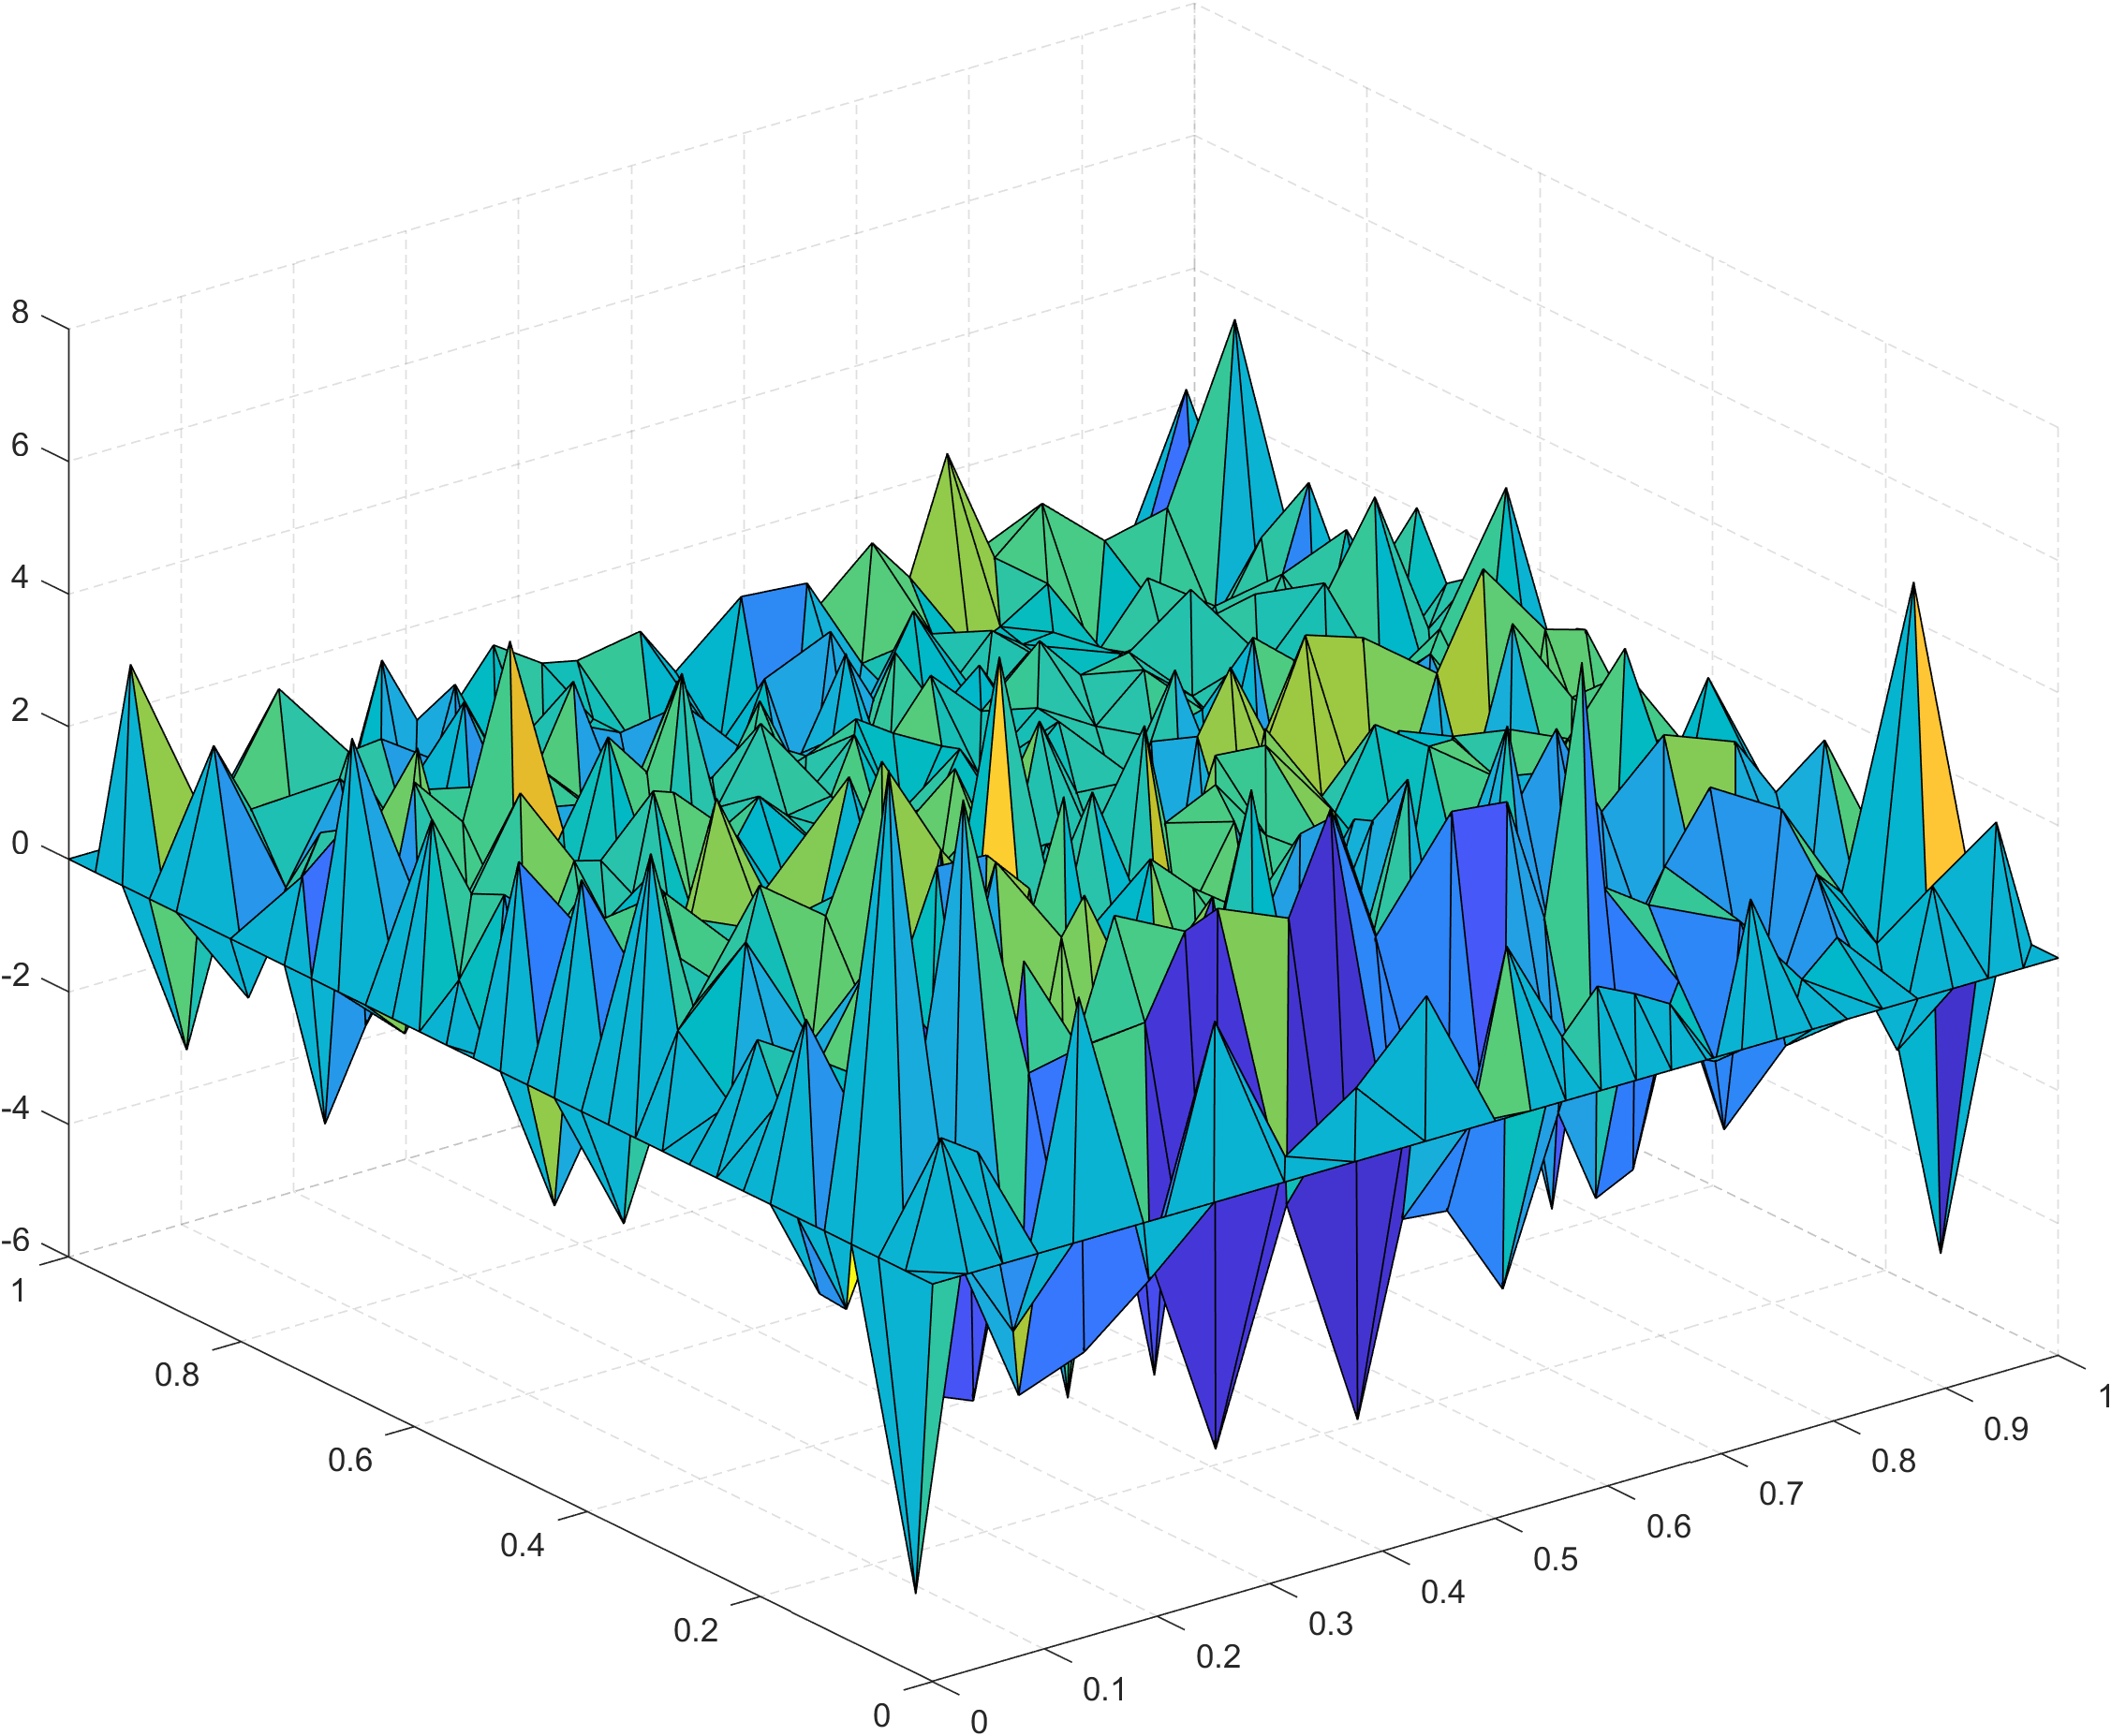
\includegraphics[width=\dimIm]{../Immagini/SDC2_SS_P2_AMax=0.005.png}
                            \caption{Coi $\mathbb{P}_2$.}
                            \label{figSDC2InstabileP2}
                        \end{subfigure}
                    }
                    \caption{Soluzione qualitativa dell'SDC2 instabile.}
                    \label{figSDC2Instabile}
                \end{figure}
                }

    
            \subsubsection{Stabilizzazione \texorpdfstring{\textit{SUPG}}{SUPG}}

                È dunque perspicua la necessità di stabilizzare il \eqref{eqSDC} e il metodo scelto per farlo è lo \textit{Streamline Upwind Petrov Galerkin}, indicato con \textit{SUPG} (si v. \cite{dispenseMEDèPA} $\S11.1.3$ per maggiori dettagli). Essa si basa sull'aggiunta lungo $\boldsymbol\beta$ di viscosità artificiale
                %
                \begin{equation}
                    \SpaziaturaMate{1}{2}{3}
                    \tau_T=
                    \left\{
                    \begin{aligned} 
                        &m_k\frac{h_T^2}{4\nu},
                        &0\le &Pe_T\le1\quad
                        \left(\parbox[c]{1.5cm}{\centering diffusione\\dominante}\right),\\[2.5pt]
                        &\frac{h_T}{2\Vert\boldsymbol\beta\Vert_T},
                        &&Pe_T\ge 1\quad
                        \left(\parbox[c]{1.5cm}{\centering convezione\\dominante}\right),
                    \end{aligned}
                    \right.
                    \label{eqViscositaArtificiale}
                \end{equation}
                %
                moltiplicata al residuo debole di un \teqref{eqPSVariazionaleDiscreto}{[PV]$_\text{h}$} avente solo Dirichlet omogeneo e funzione tèste uguale a $\boldsymbol\beta\cdot\nabla v_h$:
                %
                \begin{equation*}
                    \SpaziaturaMate{1}{2}{3}
                    r_s^T(u_h,\boldsymbol\beta\cdot\nabla v_h)\equiv a^T(u_h,\boldsymbol\beta\cdot\nabla v_h)-F^T(\boldsymbol\beta\cdot\nabla v_h),
                    \label{eqResiduoPEDiscreto}
                \end{equation*}
                ove si è indicando l'insieme d'integrazione ad apice degli operatori nelle \eqref{eqOperatoreBilinearePSVariazionale} e \eqref{eqDimIntervalliEquispaziatiScalaLog}, ossia vale
                %
                \begin{equation*}
                    \SpaziaturaMate{1}{2}{3}
                    \begin{aligned}
                        a^W(u,v)&\equiv
                        \int_W\!\!\!\nu\nabla u\cdot\nabla v
                        +\boldsymbol\beta\cdot\nabla uv
                        +\sigma uv \,\de x,\\
                        F^W(v)&\equiv
                        \int_W\!\!\!fv\, \de x,
                        \quad\text{con }W\subseteq\Omega.
                    \end{aligned}
                    \label{eqOperatoreBilinearePVRidefinizioneSottoinsieme}
                \end{equation*}
                %
                Ciò trasforma il \teqref{eqPSVariazionaleDiscreto}{[PV]$_\text{h}$} nel problema
                %    
                \begin{equation*}
                    \SpaziaturaMate{1}{2}{3}
                    [\text{PV}]^\text{s}_\text{h}
                    \left\{
                    \begin{aligned}
                        &\text{Trovare }u_h\in V_h\text{ tale che}\\[5pt]
                        &a^\Omega(u_h,v_h)+\sum_{T\in\mathcal T_h}\tau_Tr^T_s(u_h,\boldsymbol\beta\cdot\nabla v_h)\\
                        &=F^\Omega(v_h)+G^{\Gamma_N}(v_h)-a^\Omega(Rg_D,v_h),\\[5pt]
                        &\forall v_h\in V_h,
                    \end{aligned}
                    \right.
                    \label{eqPVDiscretoStabilizzato}
                \end{equation*}
                %
                la cui principale differenza con quello originale è quella di cambiare le funzioni teste rendendole piú sensibili sopravento rispetto alla direzione di $\boldsymbol\beta$ (da cui il nome \textit{Streamline Upwind}), come illustrato graficamente e qualitativamente nella Fig. \ref{figFunzioniTestePetrovGalerkin}.
                
                \begin{figure}[t]
                    \centering
                    \setlength{\belowcaptionskip}{-0.5cm}
                    \begin{tikzpicture}[scale=0.95]
                    
                            % Primo grafico: funzione lagrangiana
                        \draw (0,0) node[below left] {\scriptsize$0$};
                        \draw[->] (-0.25,0) -- (2.5,0) node[below] {$x$}; % Asse x
                        \draw[->] (0,-1.5) -- (0,1.5) node[left] {$y$};  % Asse y

                            % beta
                        \pgfmathsetmacro{\xiBeta}{0.15}
                        \pgfmathsetmacro{\yBeta}{-0.9}
                        \pgfmathsetmacro{\lBeta}{0.65}
                        \pgfmathsetmacro{\xfBeta}{\xiBeta+\lBeta}
                        \draw[->] (\xiBeta,\yBeta) -- (\xfBeta,\yBeta) node[midway,above]
                                  {\scriptsize$\SpaziaturaMate{1}{2}{3}\boldsymbol\beta>0$};
                        
                        \draw[thick,blue] (0,0) -- (1,1)
                                       -- (2,0) node[below,black] {\scriptsize$1$};       % Funzione lagrangiana
                        \draw[dashed] (1,0) node[below] {\scriptsize$0.5$} -- (1,1);  % Linea ausiliaria
                        \draw[dashed] (0,1) node[left] {\scriptsize$1$} -- (1,1);  % Linea ausiliaria

                            % Titolo
                        \node at (1,-1.75) {$\varphi_j$};
                        
                            % Secondo grafico: funzione gradino
                        \begin{scope}[xshift=3cm] % Trasla il grafico
                            \draw[->] (-0.25,0) -- (2.5,0) node[below] {$x$}; % Asse x
                            \draw[->] (0,-1.5) -- (0,1.5) node[left] {$y$};  % Asse y
                            
                            \draw[thick,red] (0,1) -- (1,1);
                            \draw[dashed] (1,1) -- (1,-1);
                            \draw[thick,red] (1,-1) -- (2,-1); % Gradino
                            \draw[dashed] (2,0) -- (2,-1);
                            \draw (1,0) node[below,fill=white] {\scriptsize$0.5$};
                            \draw (2,0) node[below,fill=white] {\scriptsize$1$};
                            \draw (0,1) node[left] {\scriptsize$1$};
                            
                                % beta
                            \draw[->] (\xiBeta,\yBeta) -- (\xfBeta,\yBeta) node[midway,above]
                                      {\scriptsize$\SpaziaturaMate{1}{2}{3}\boldsymbol\beta>0$};
                                  
                            % Titolo
                            \node at (1,-1.75) {$\boldsymbol\beta\cdot\nabla\varphi_j$};
                        \end{scope}
                        
                            % Terzo grafico: somma delle due
                        \begin{scope}[xshift=6cm] % Trasla il grafico
                            \draw[->] (-0.25,0) -- (2.5,0) node[below] {$x$}; % Asse x
                            \draw[->] (0,-1.5) -- (0,1.5) node[left] {$y$};    % Asse y
                            
                            \draw[thick,green!70!black] 
                                (0,1) -- (1,2); % Somma
                            \draw[dashed] (1,0) -- (1,2);
                            \draw[thick,green!70!black] 
                                (1,0) -- (2,-1); % Somma
                            \draw[dashed] (2,0) -- (2,-1);
                            \draw (1,0) node[below] {\scriptsize$0.5$};
                            \draw (2,0) node[below,fill=white] {\scriptsize$1$};
                            \draw (0,1) node[left] {\scriptsize$1$};
                            
                                % beta
                            \draw[->] (\xiBeta,\yBeta) -- (\xfBeta,\yBeta) node[midway,above]
                                      {\scriptsize$\SpaziaturaMate{1}{2}{3}\boldsymbol\beta>0$};
                                      
                            % Titolo
                            \node at (1,-1.75) {$\varphi_j+\boldsymbol\beta\cdot\nabla\varphi_j$};
                        \end{scope}
                    
                    \end{tikzpicture}
                    \caption{Funzioni tèste nel metodo \textit{SUPG}.}
                    \label{figFunzioniTestePetrovGalerkin}
                \end{figure}


                %%%%%%%%%%%%%%%%%%
                %%% Infopagine %%%
                %%%%%%%%%%%%%%%%%%
                \begin{figure*}[p]
                    \newcommand{\distR}{\vspace{15pt}} % Distanza tra le righe
                    
                    \newcommand{\lungSF}{0.33\textwidth}
                    \newcommand{\dimIm}{4cm}
                    \makebox[\linewidth][c]{
                        \begin{subfigure}[t]{\lungSF}
                            \centering
                            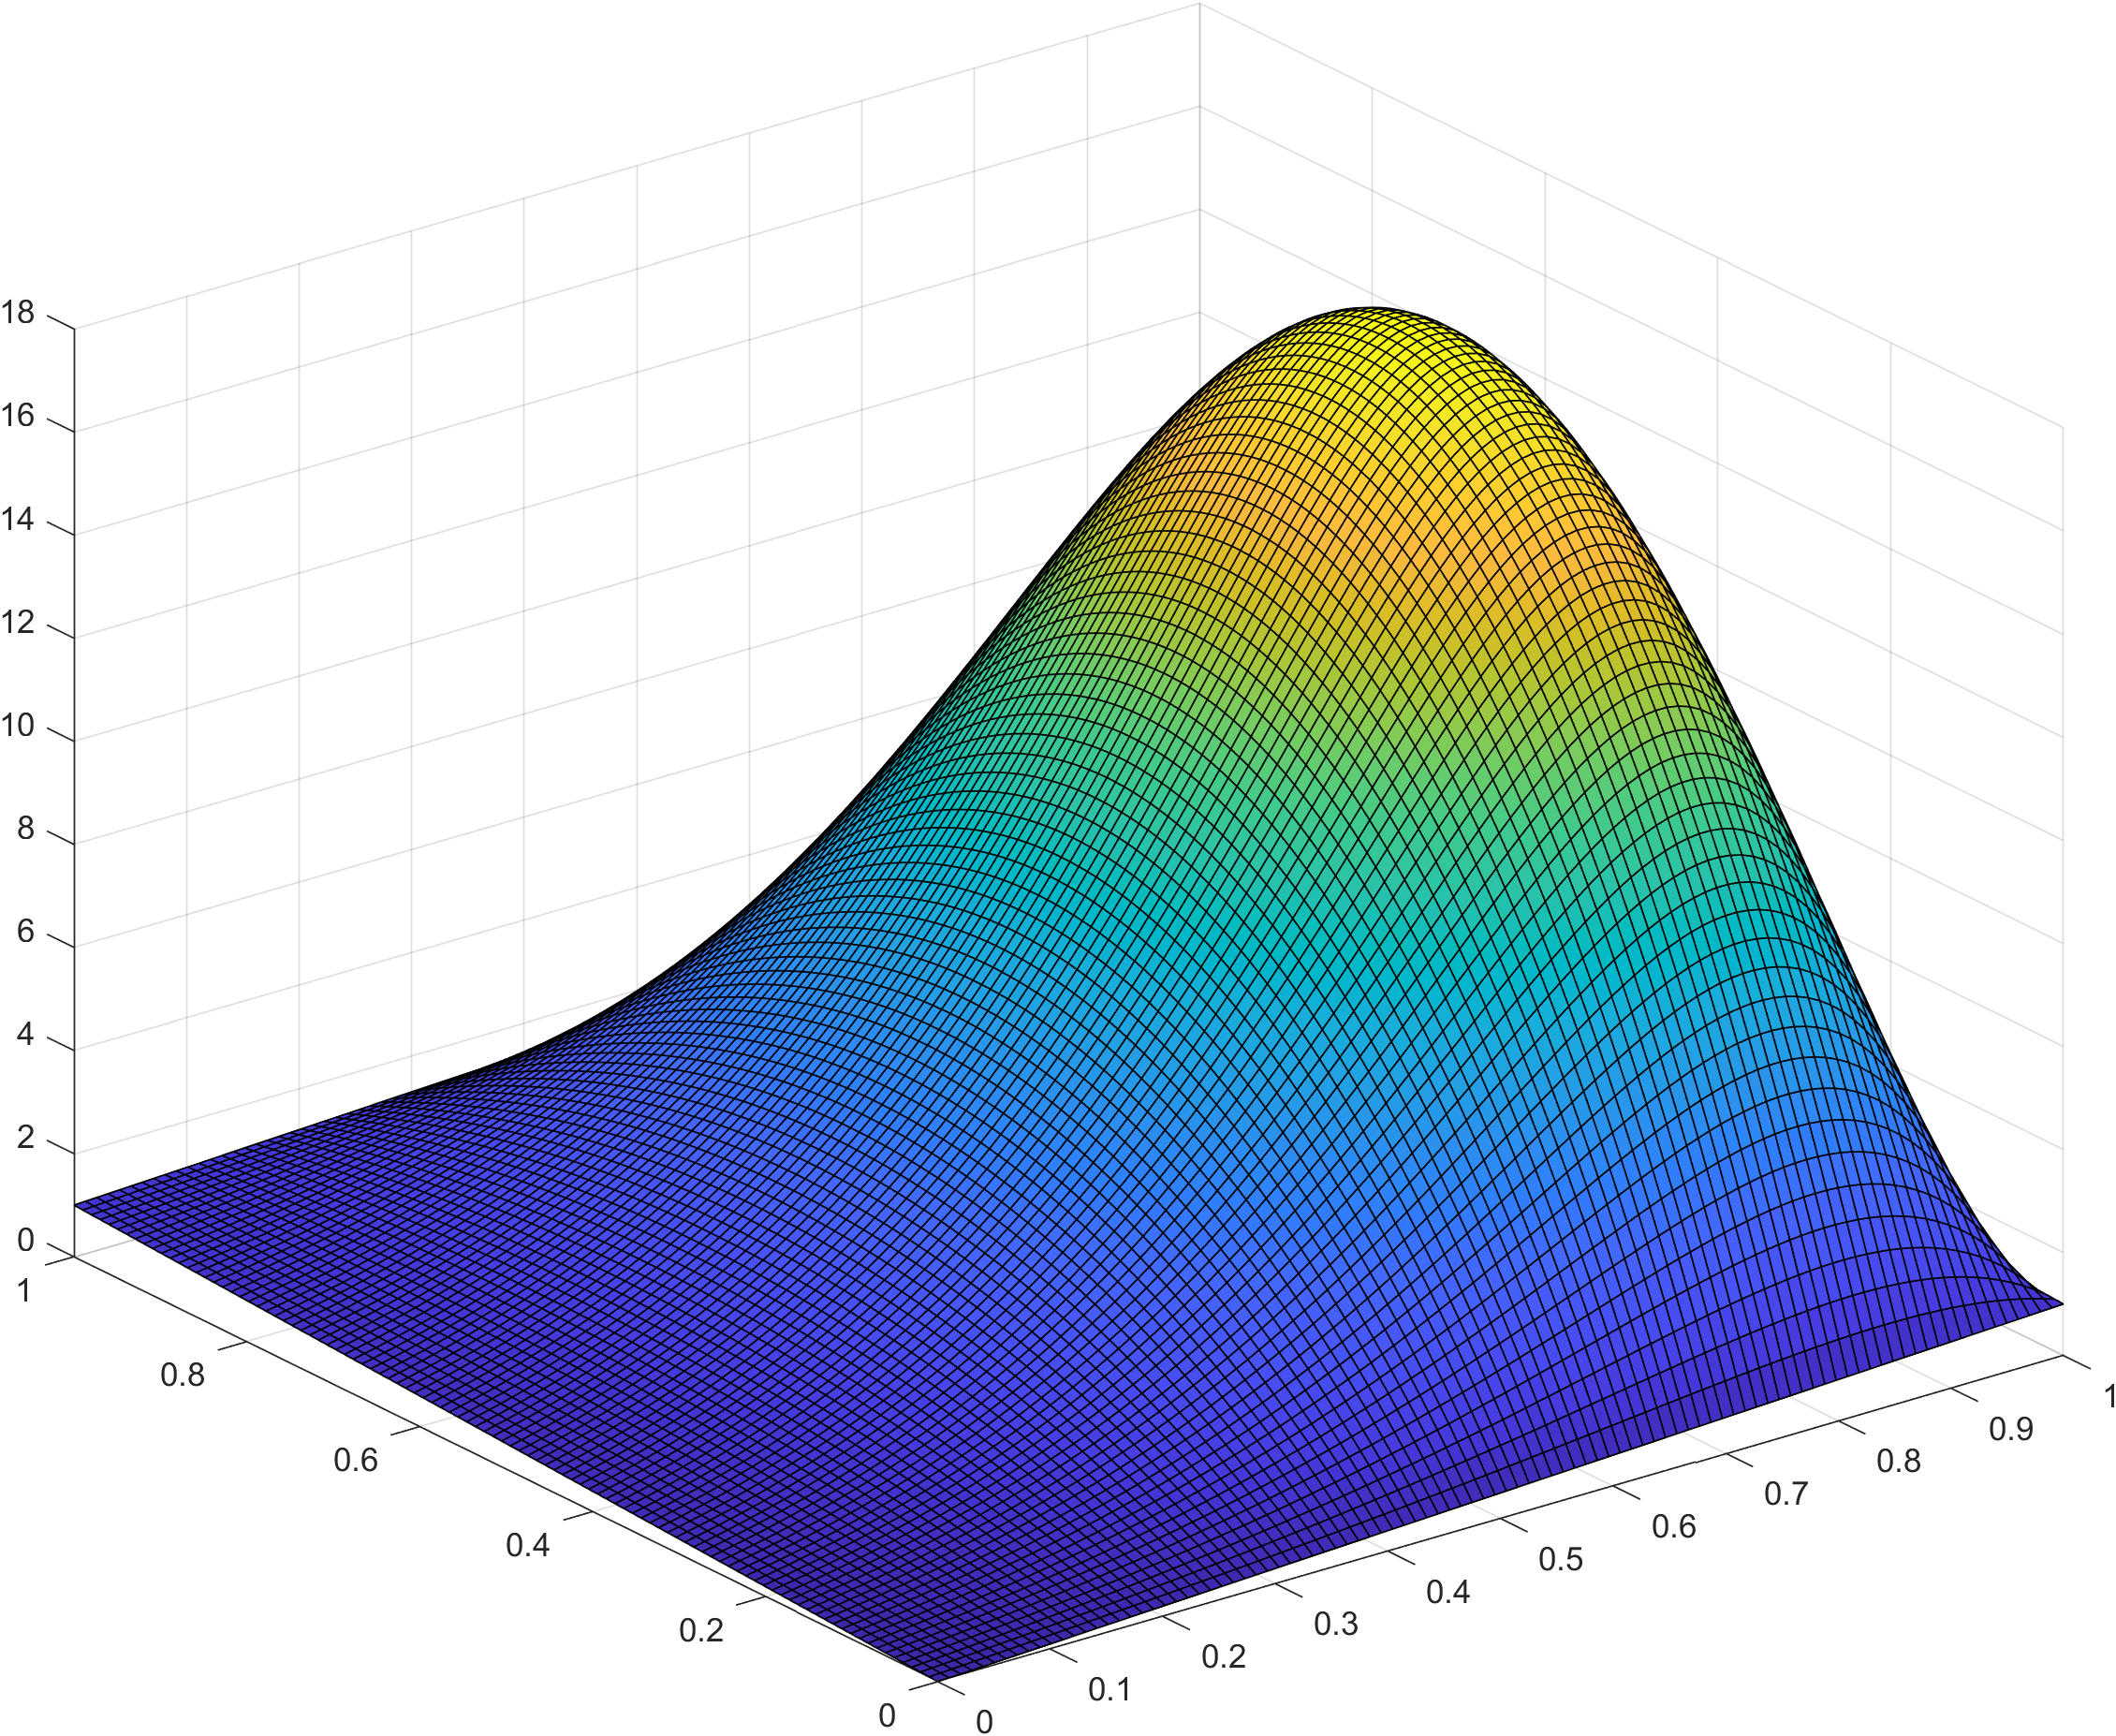
\includegraphics[height=\dimIm]{../Immagini/SDC1_SE_NPunti=100.png}
                            \caption{Soluzione esatta.}
                            \label{figSDC1TriangolazioniEsatta}
                        \end{subfigure}
                        \begin{subfigure}[t]{\lungSF}
                            \centering
                            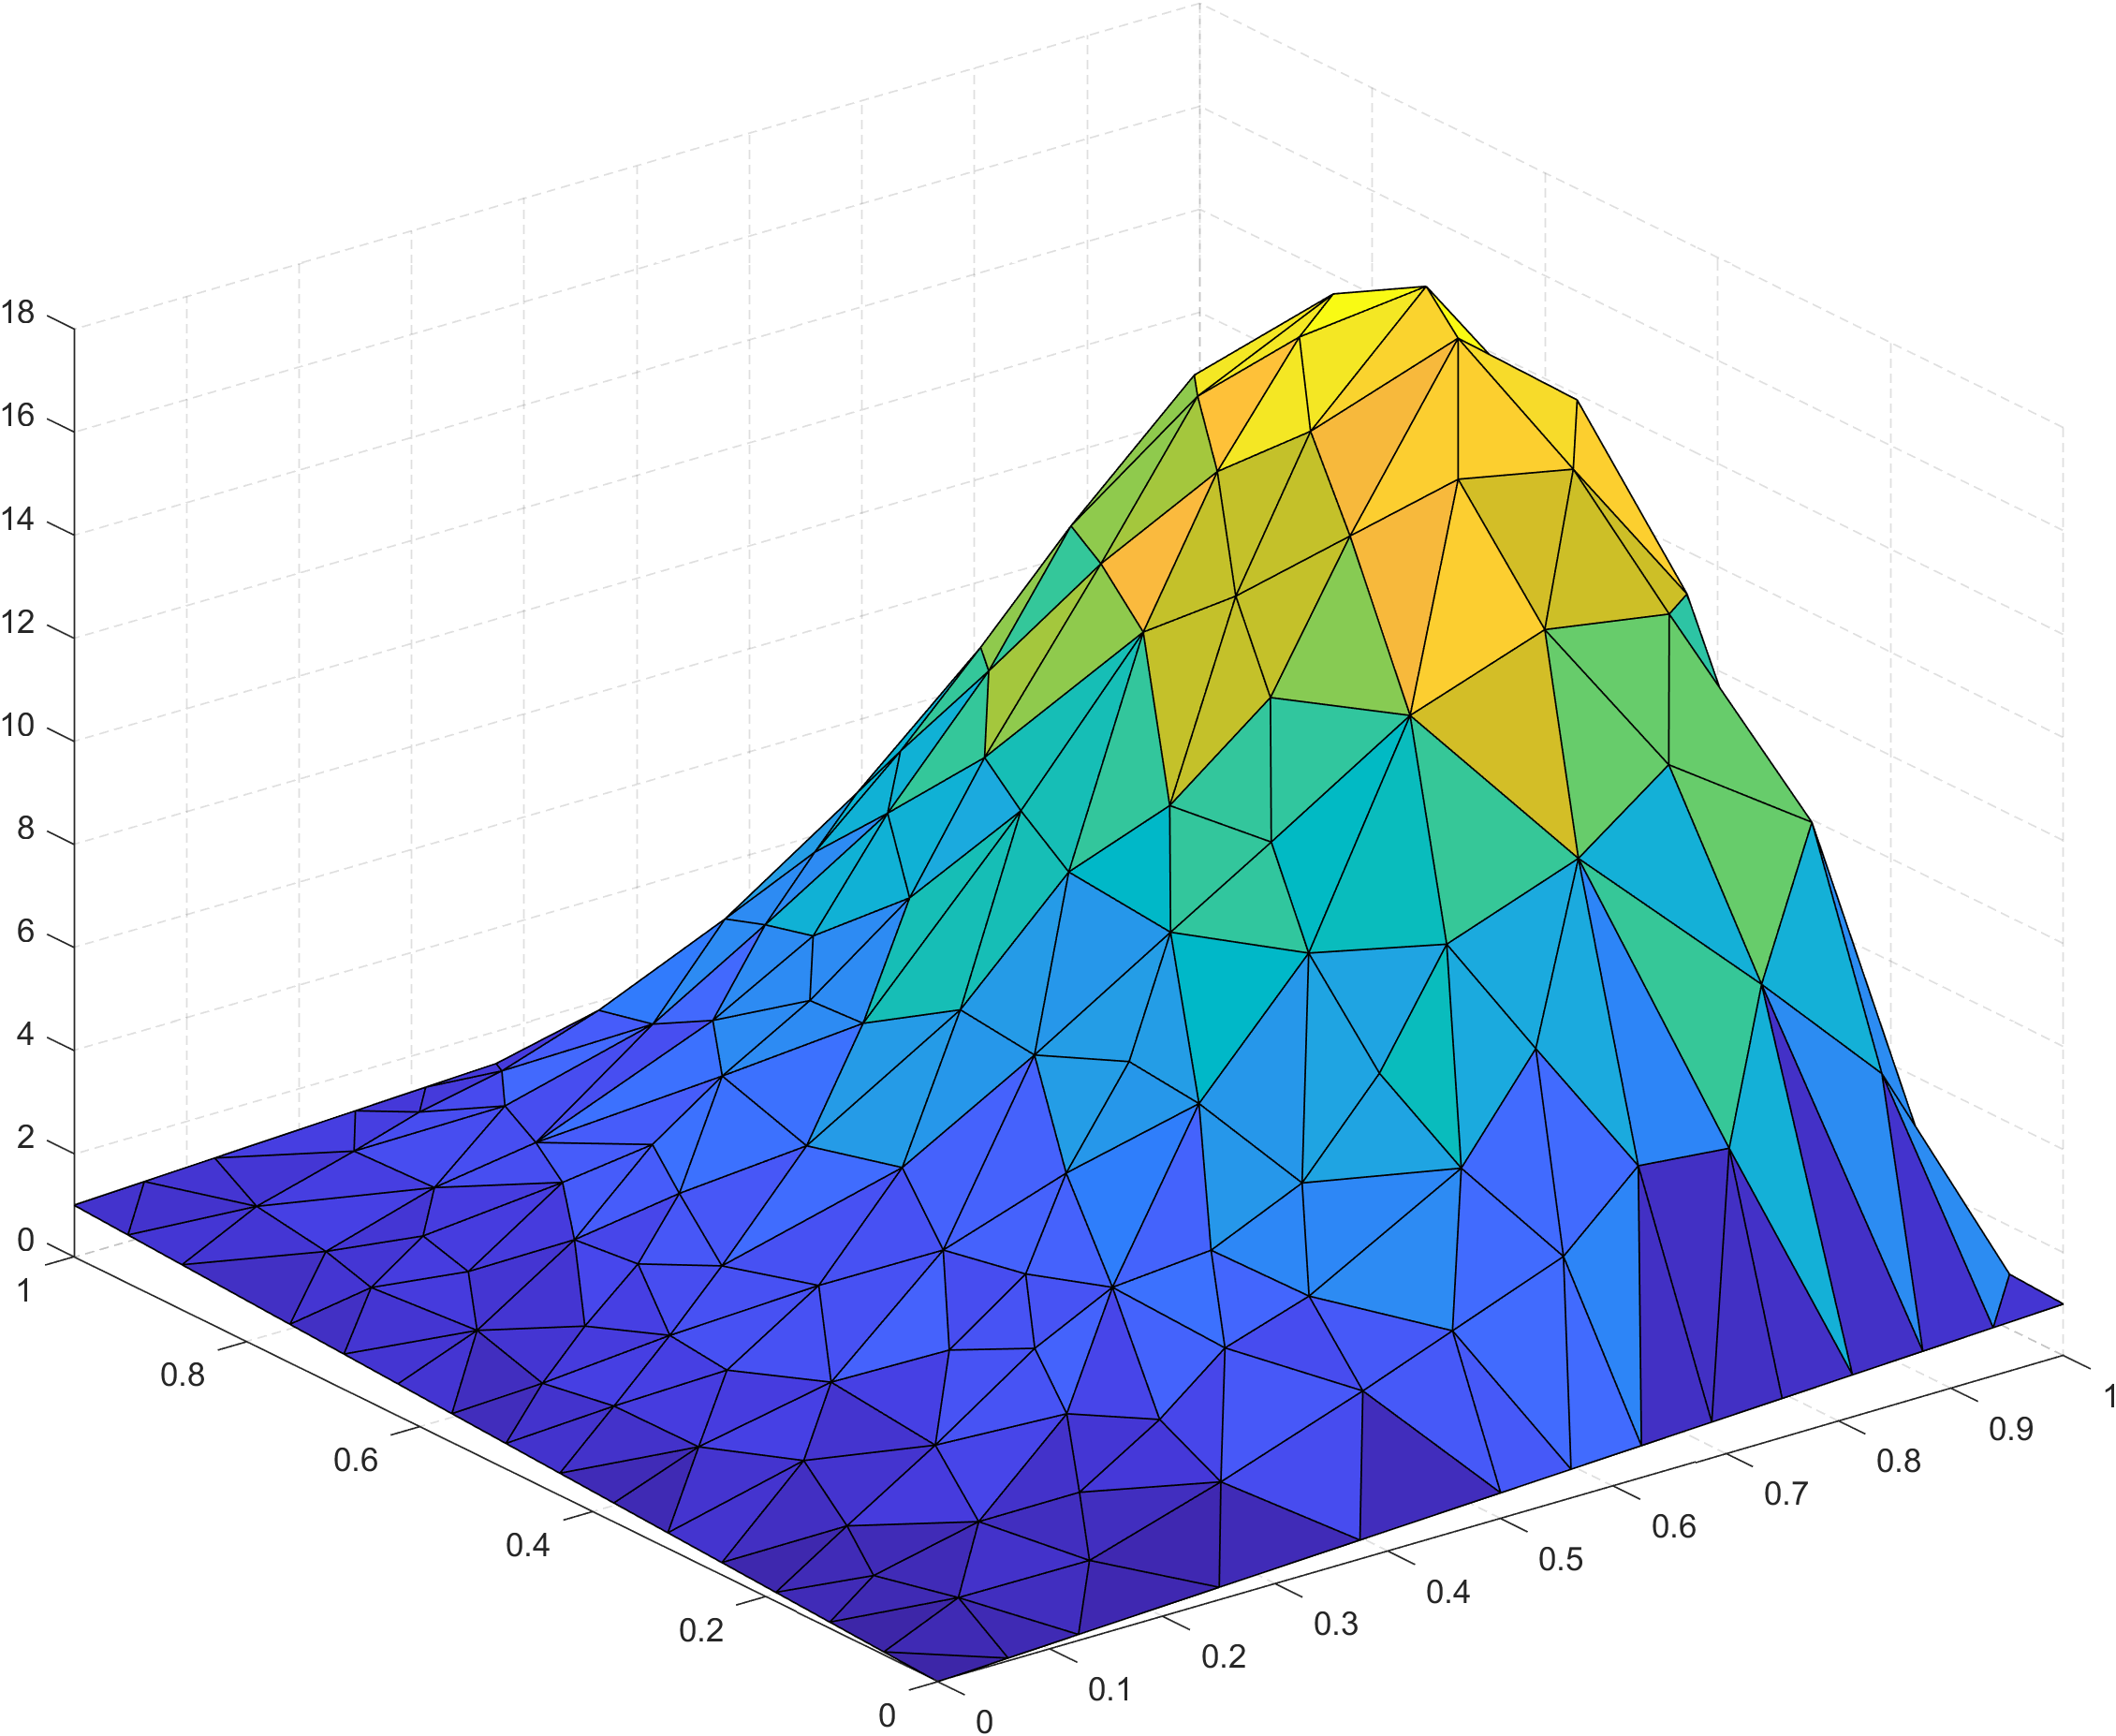
\includegraphics[height=\dimIm]{../Immagini/SDC1_CS_P1_AMax=0.005.png}
                            \caption{Soluzione qualitativa coi $\mathbb{P}_1$ ed \textit{SUPG}.}
                            \label{figSDC1TriangolazioniApprossimataP1}
                        \end{subfigure}
                        \begin{subfigure}[t]{\lungSF}
                            \centering
                            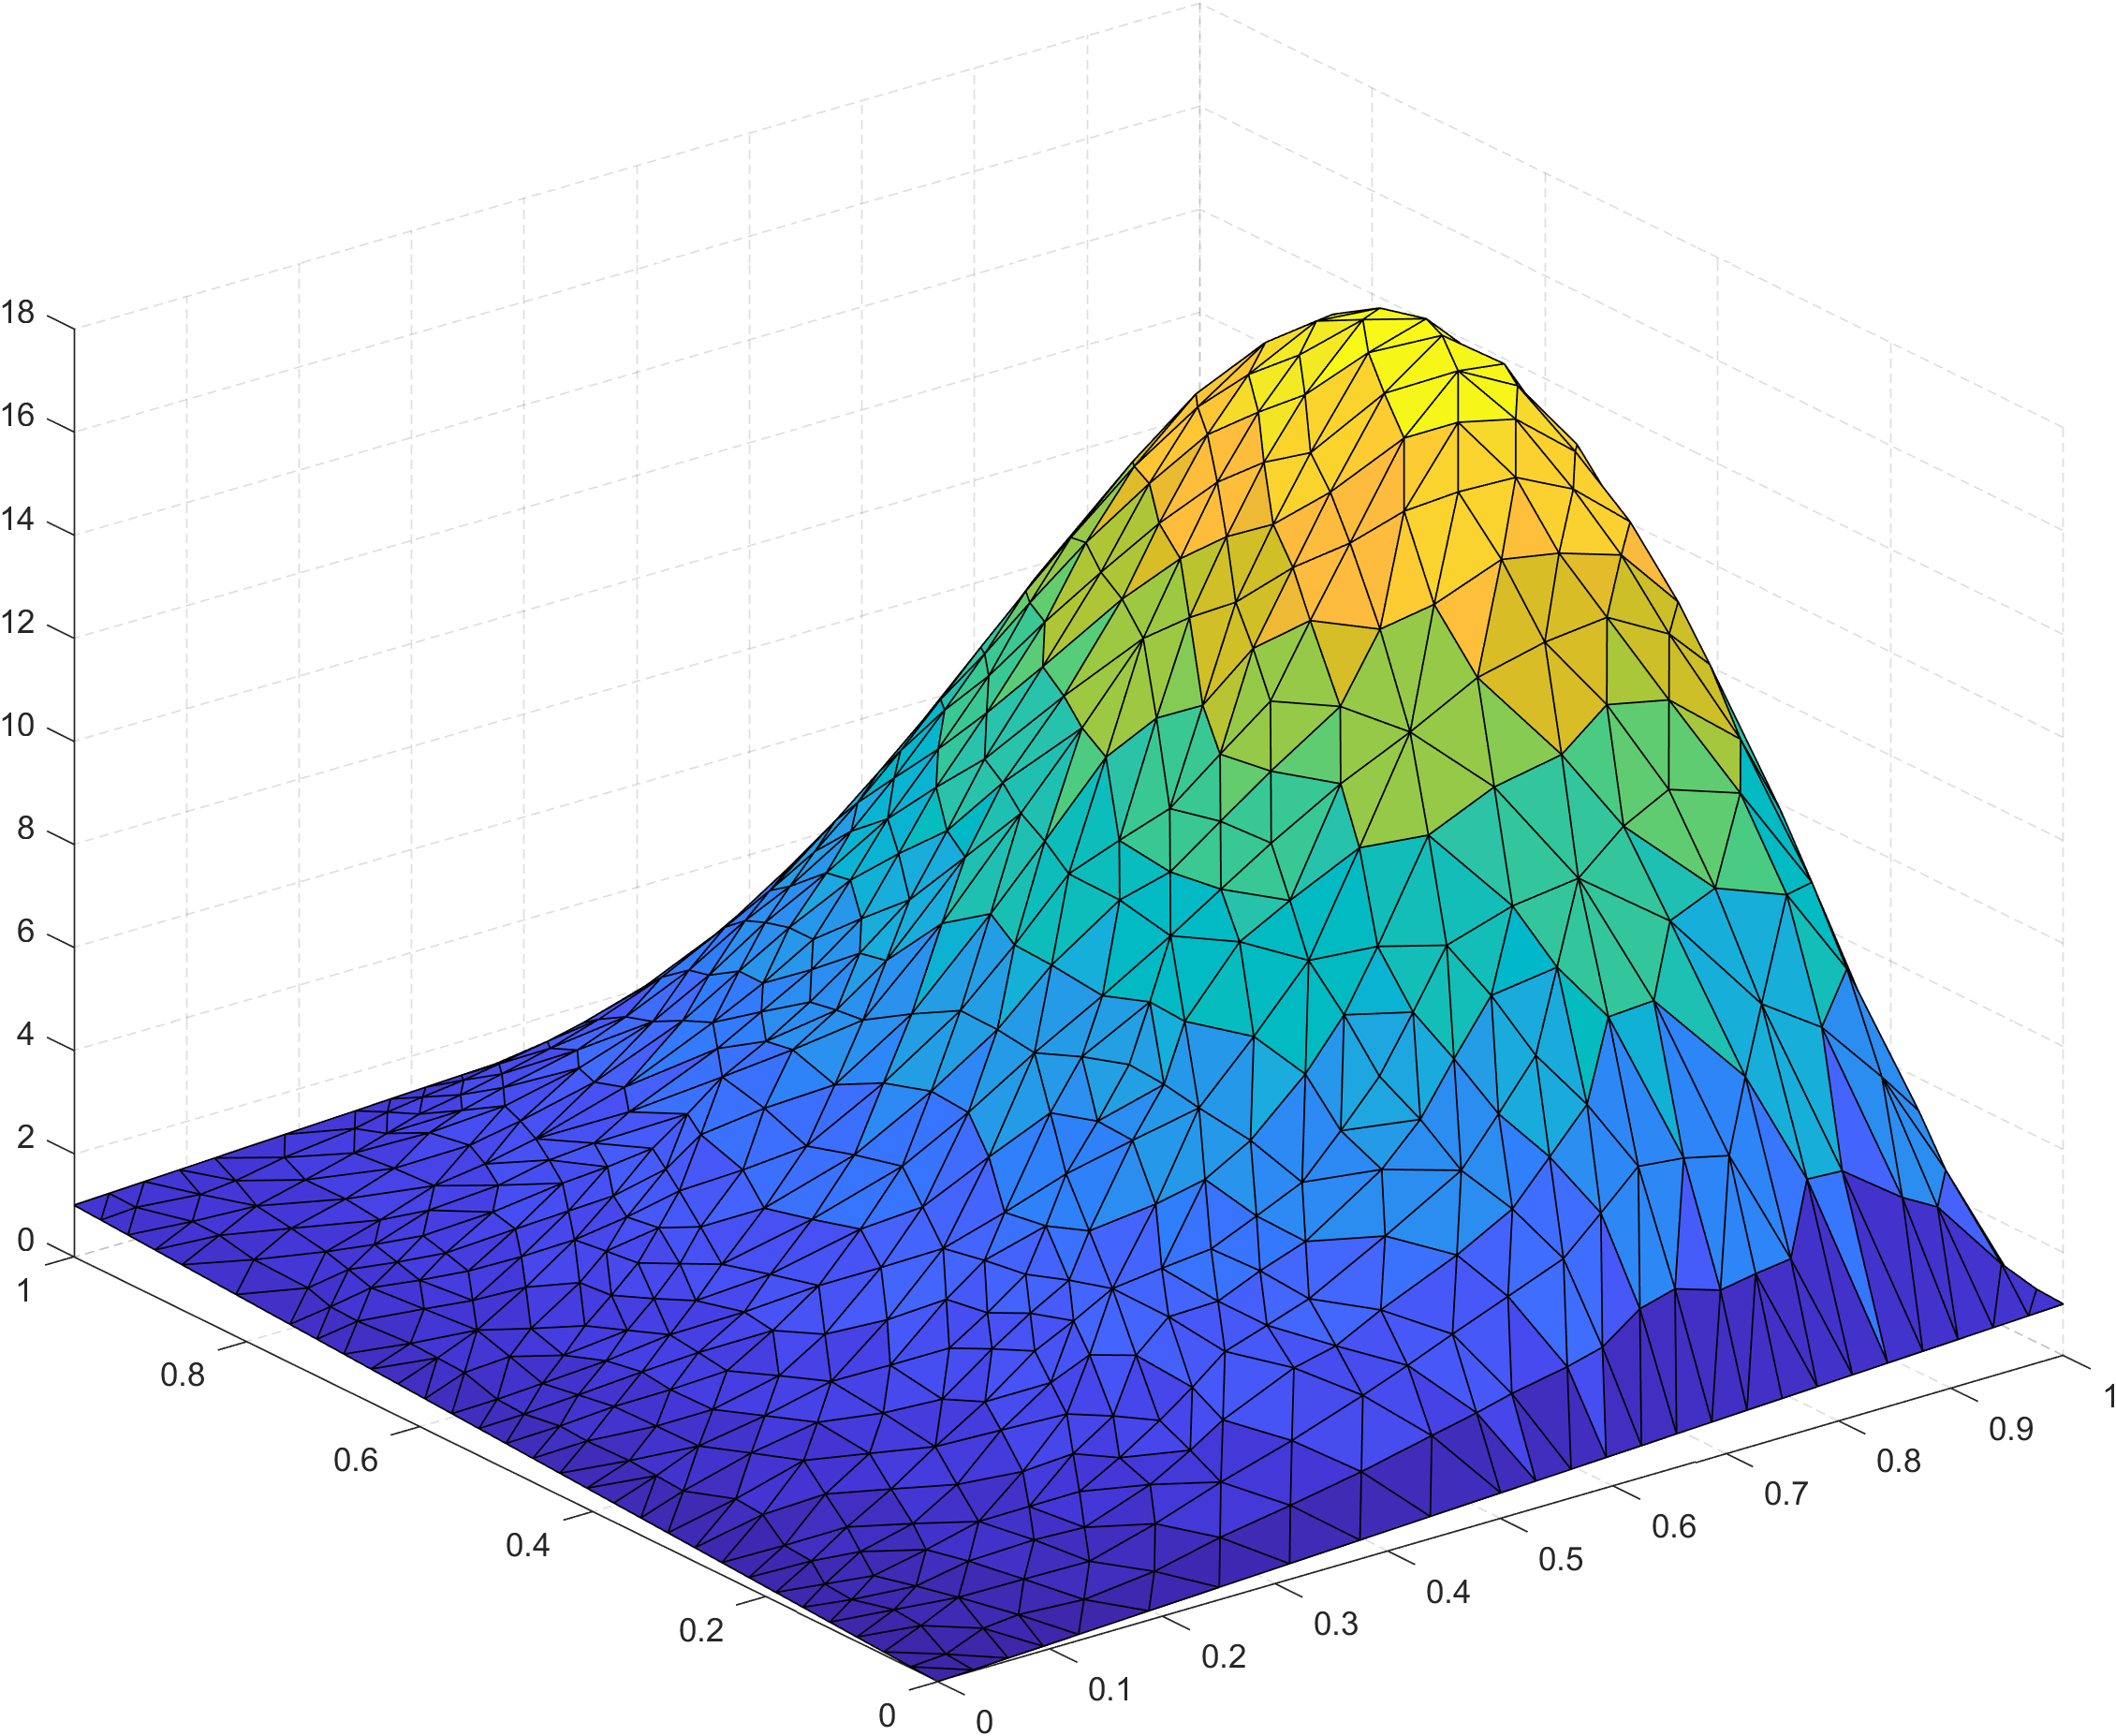
\includegraphics[height=\dimIm]{../Immagini/SDC1_CS_P2_AMax=0.005.png}
                            \caption{Soluzione qualitativa coi $\mathbb{P}_2$ ed \textit{SUPG}.}
                            \label{figSDC1TriangolazioniApprossimataP2}
                        \end{subfigure}
                    }
                    \distR
        
                    \renewcommand{\lungSF}{.5\linewidth}
                    \renewcommand{\dimIm}{\linewidth}
                    \newcommand{\distC}{\hspace{7.5pt}} % Distanza tra le colonne
                    \makebox[\linewidth][c]{
                        \begin{subfigure}[t]{\lungSF}
                            \centering
                            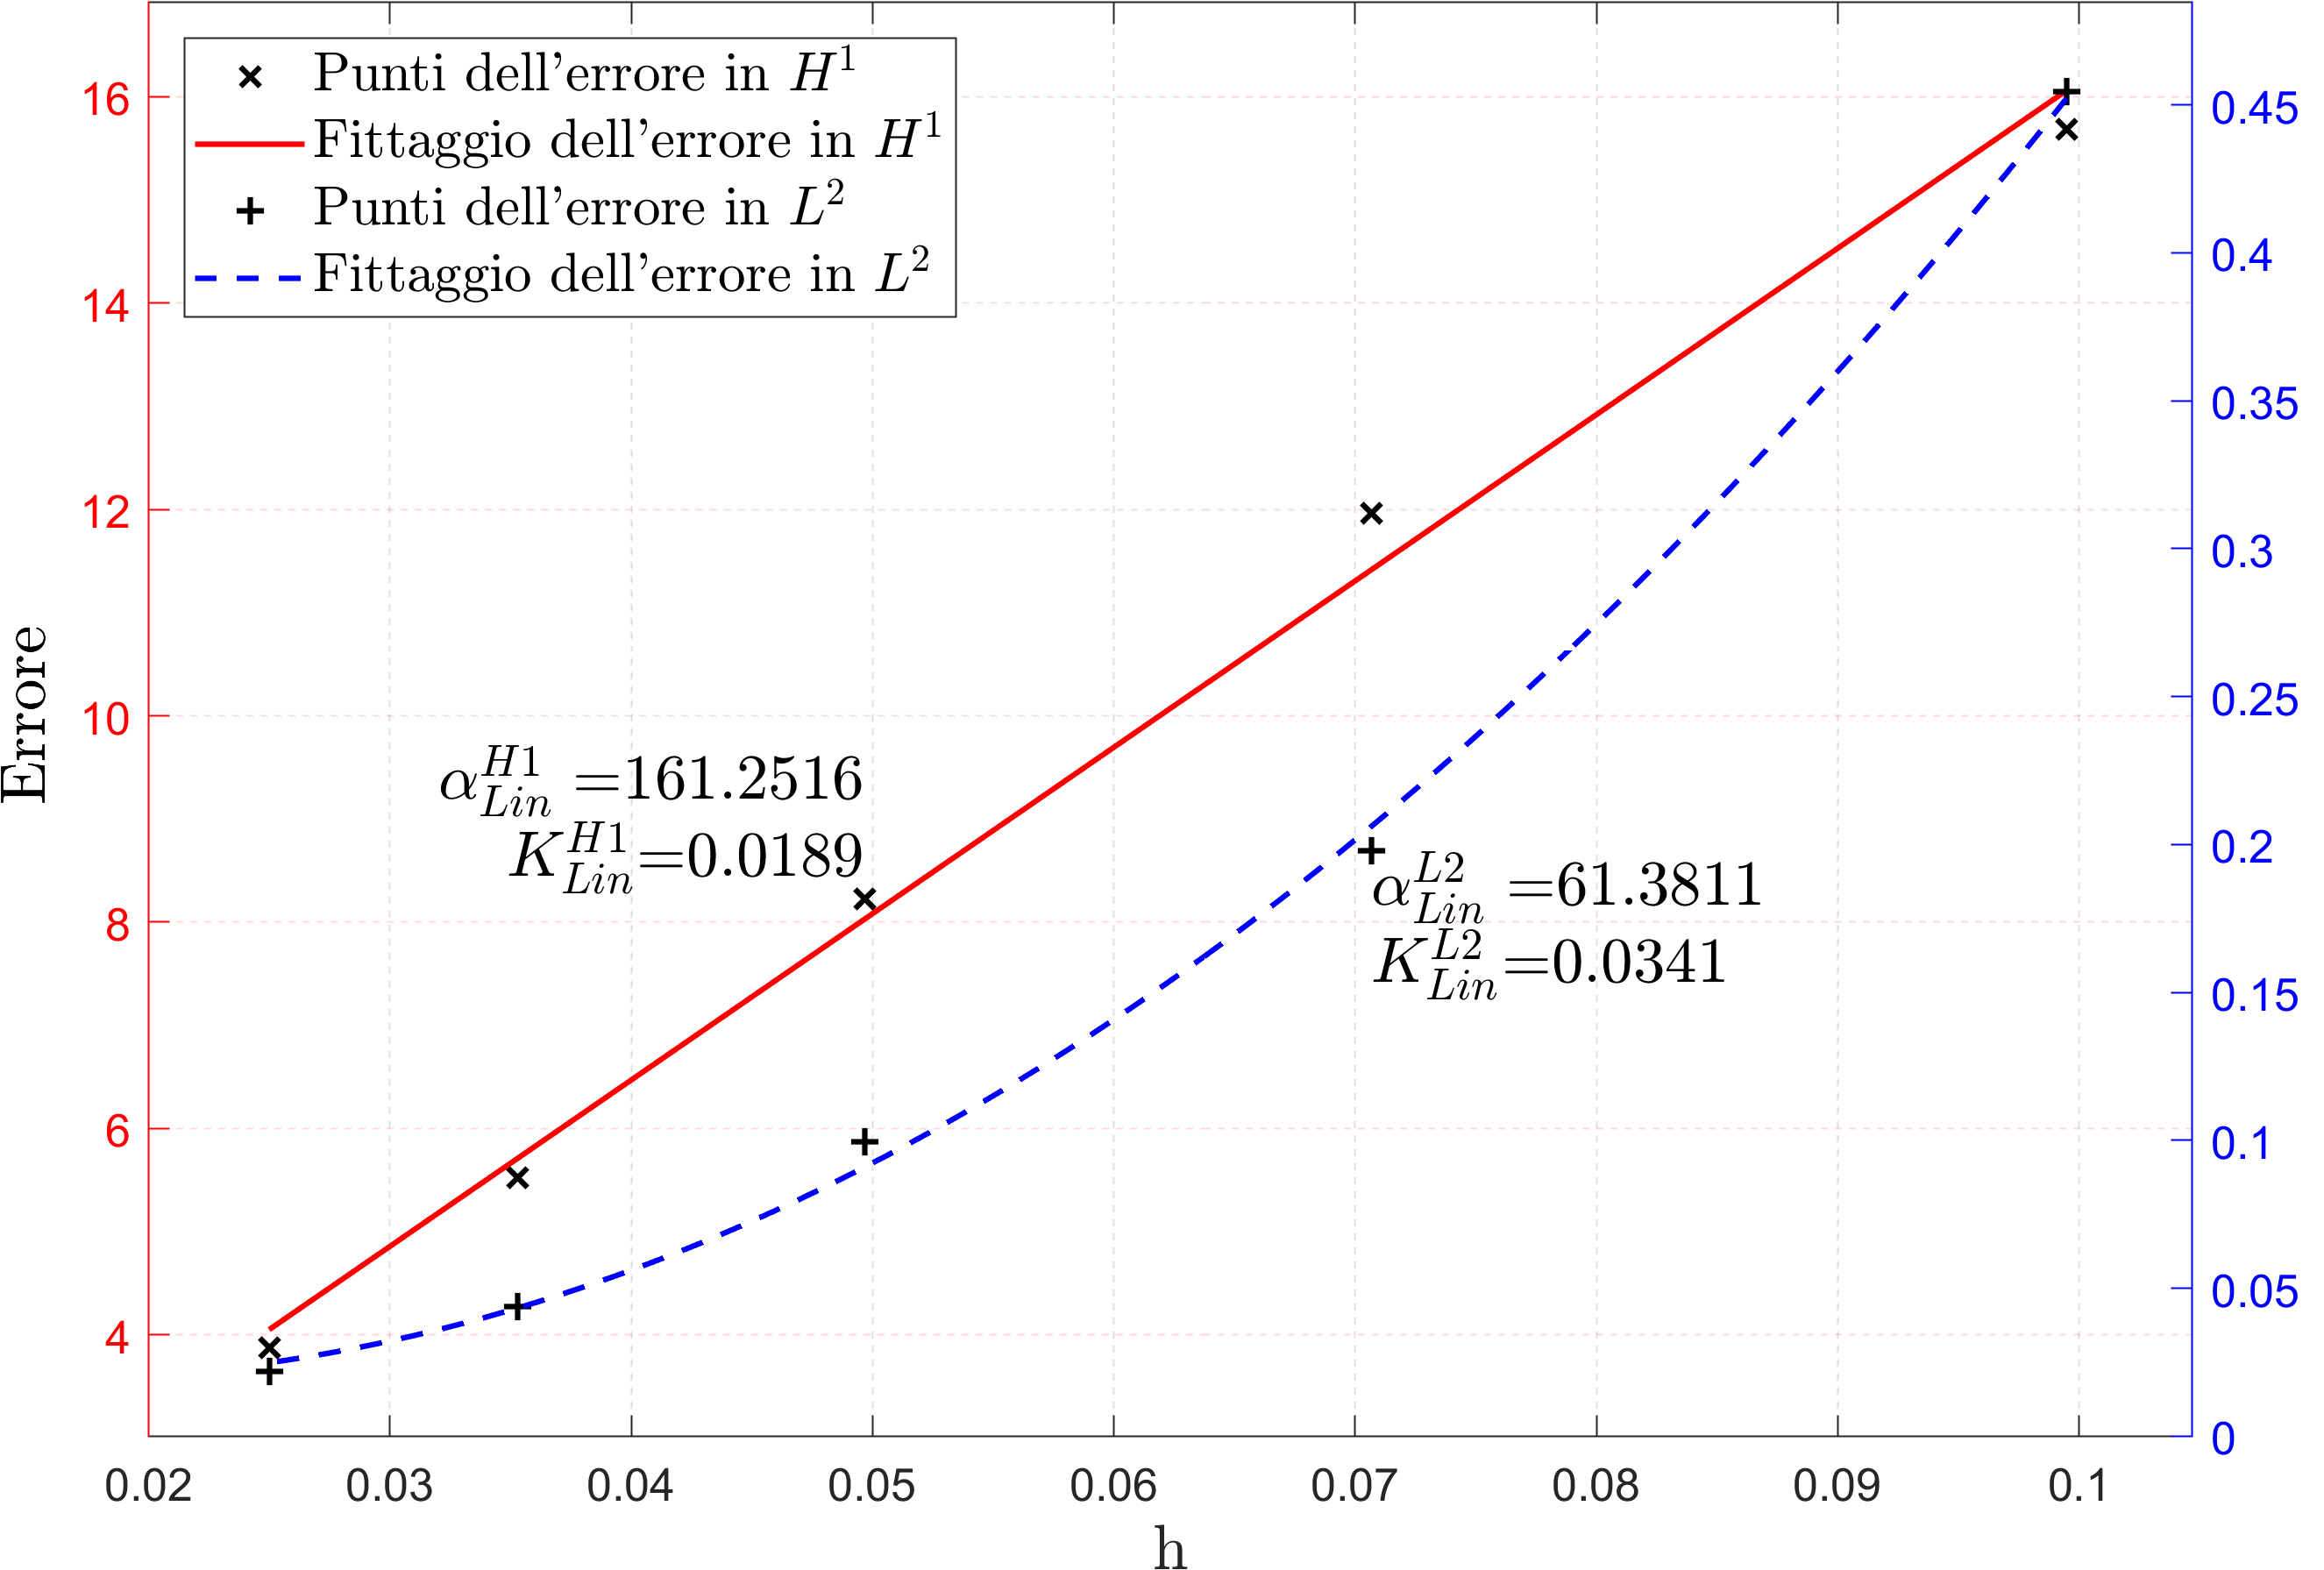
\includegraphics[width=\dimIm]{../Immagini/SDC1_P1_CS_ErrLin_AMax=0.01_NSim=5.png}
                        \caption{Errore dei $\mathbb{P}_1$ in scala lineare con \textit{SUPG}.}
                        \label{figSDC1ErroreP1Lin}
                        \end{subfigure}
                        \distC
                        \begin{subfigure}[t]{\lungSF}
                            \centering
                            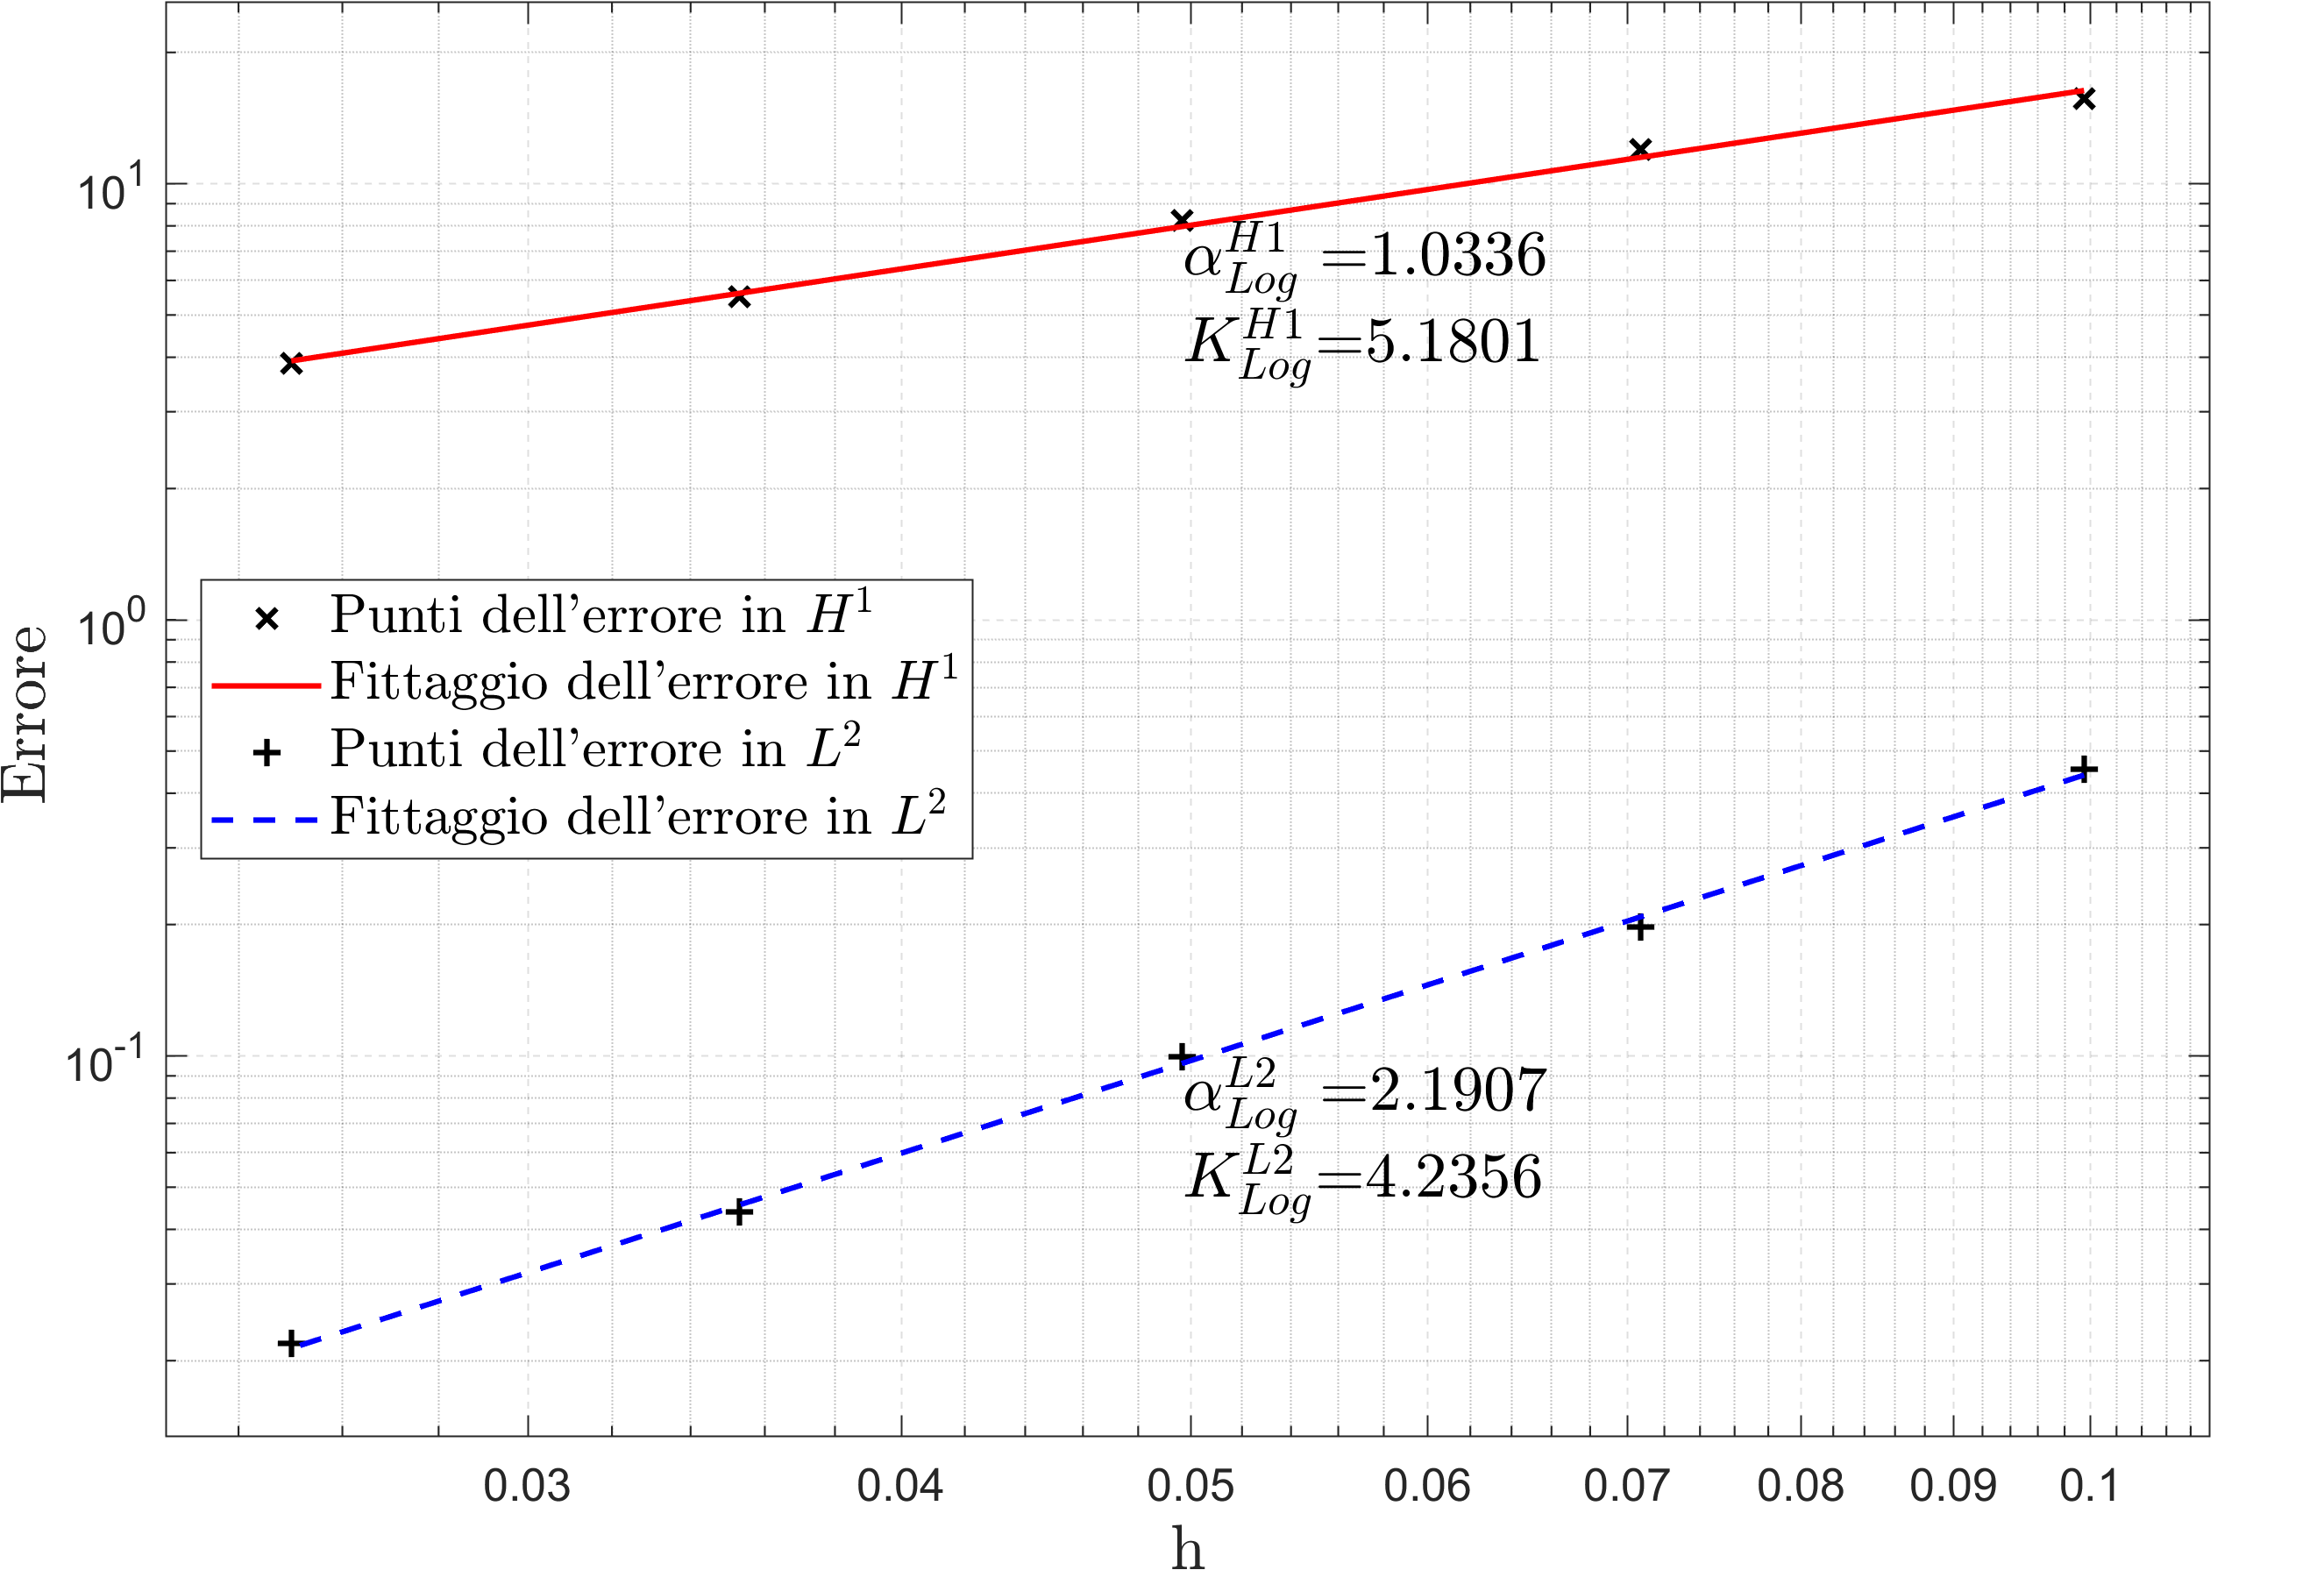
\includegraphics[width=\dimIm]{../Immagini/SDC1_P1_CS_ErrLog_AMax=0.01_NSim=5.png}
                        \caption{Errore dei $\mathbb{P}_1$ in scala logaritmica con \textit{SUPG}.}
                        \label{figSDC1ErroreP1Log}
                        \end{subfigure}
                    }
                    \distR
        
                    \makebox[\linewidth][c]{
                        \begin{subfigure}[t]{\lungSF}
                            \centering
                            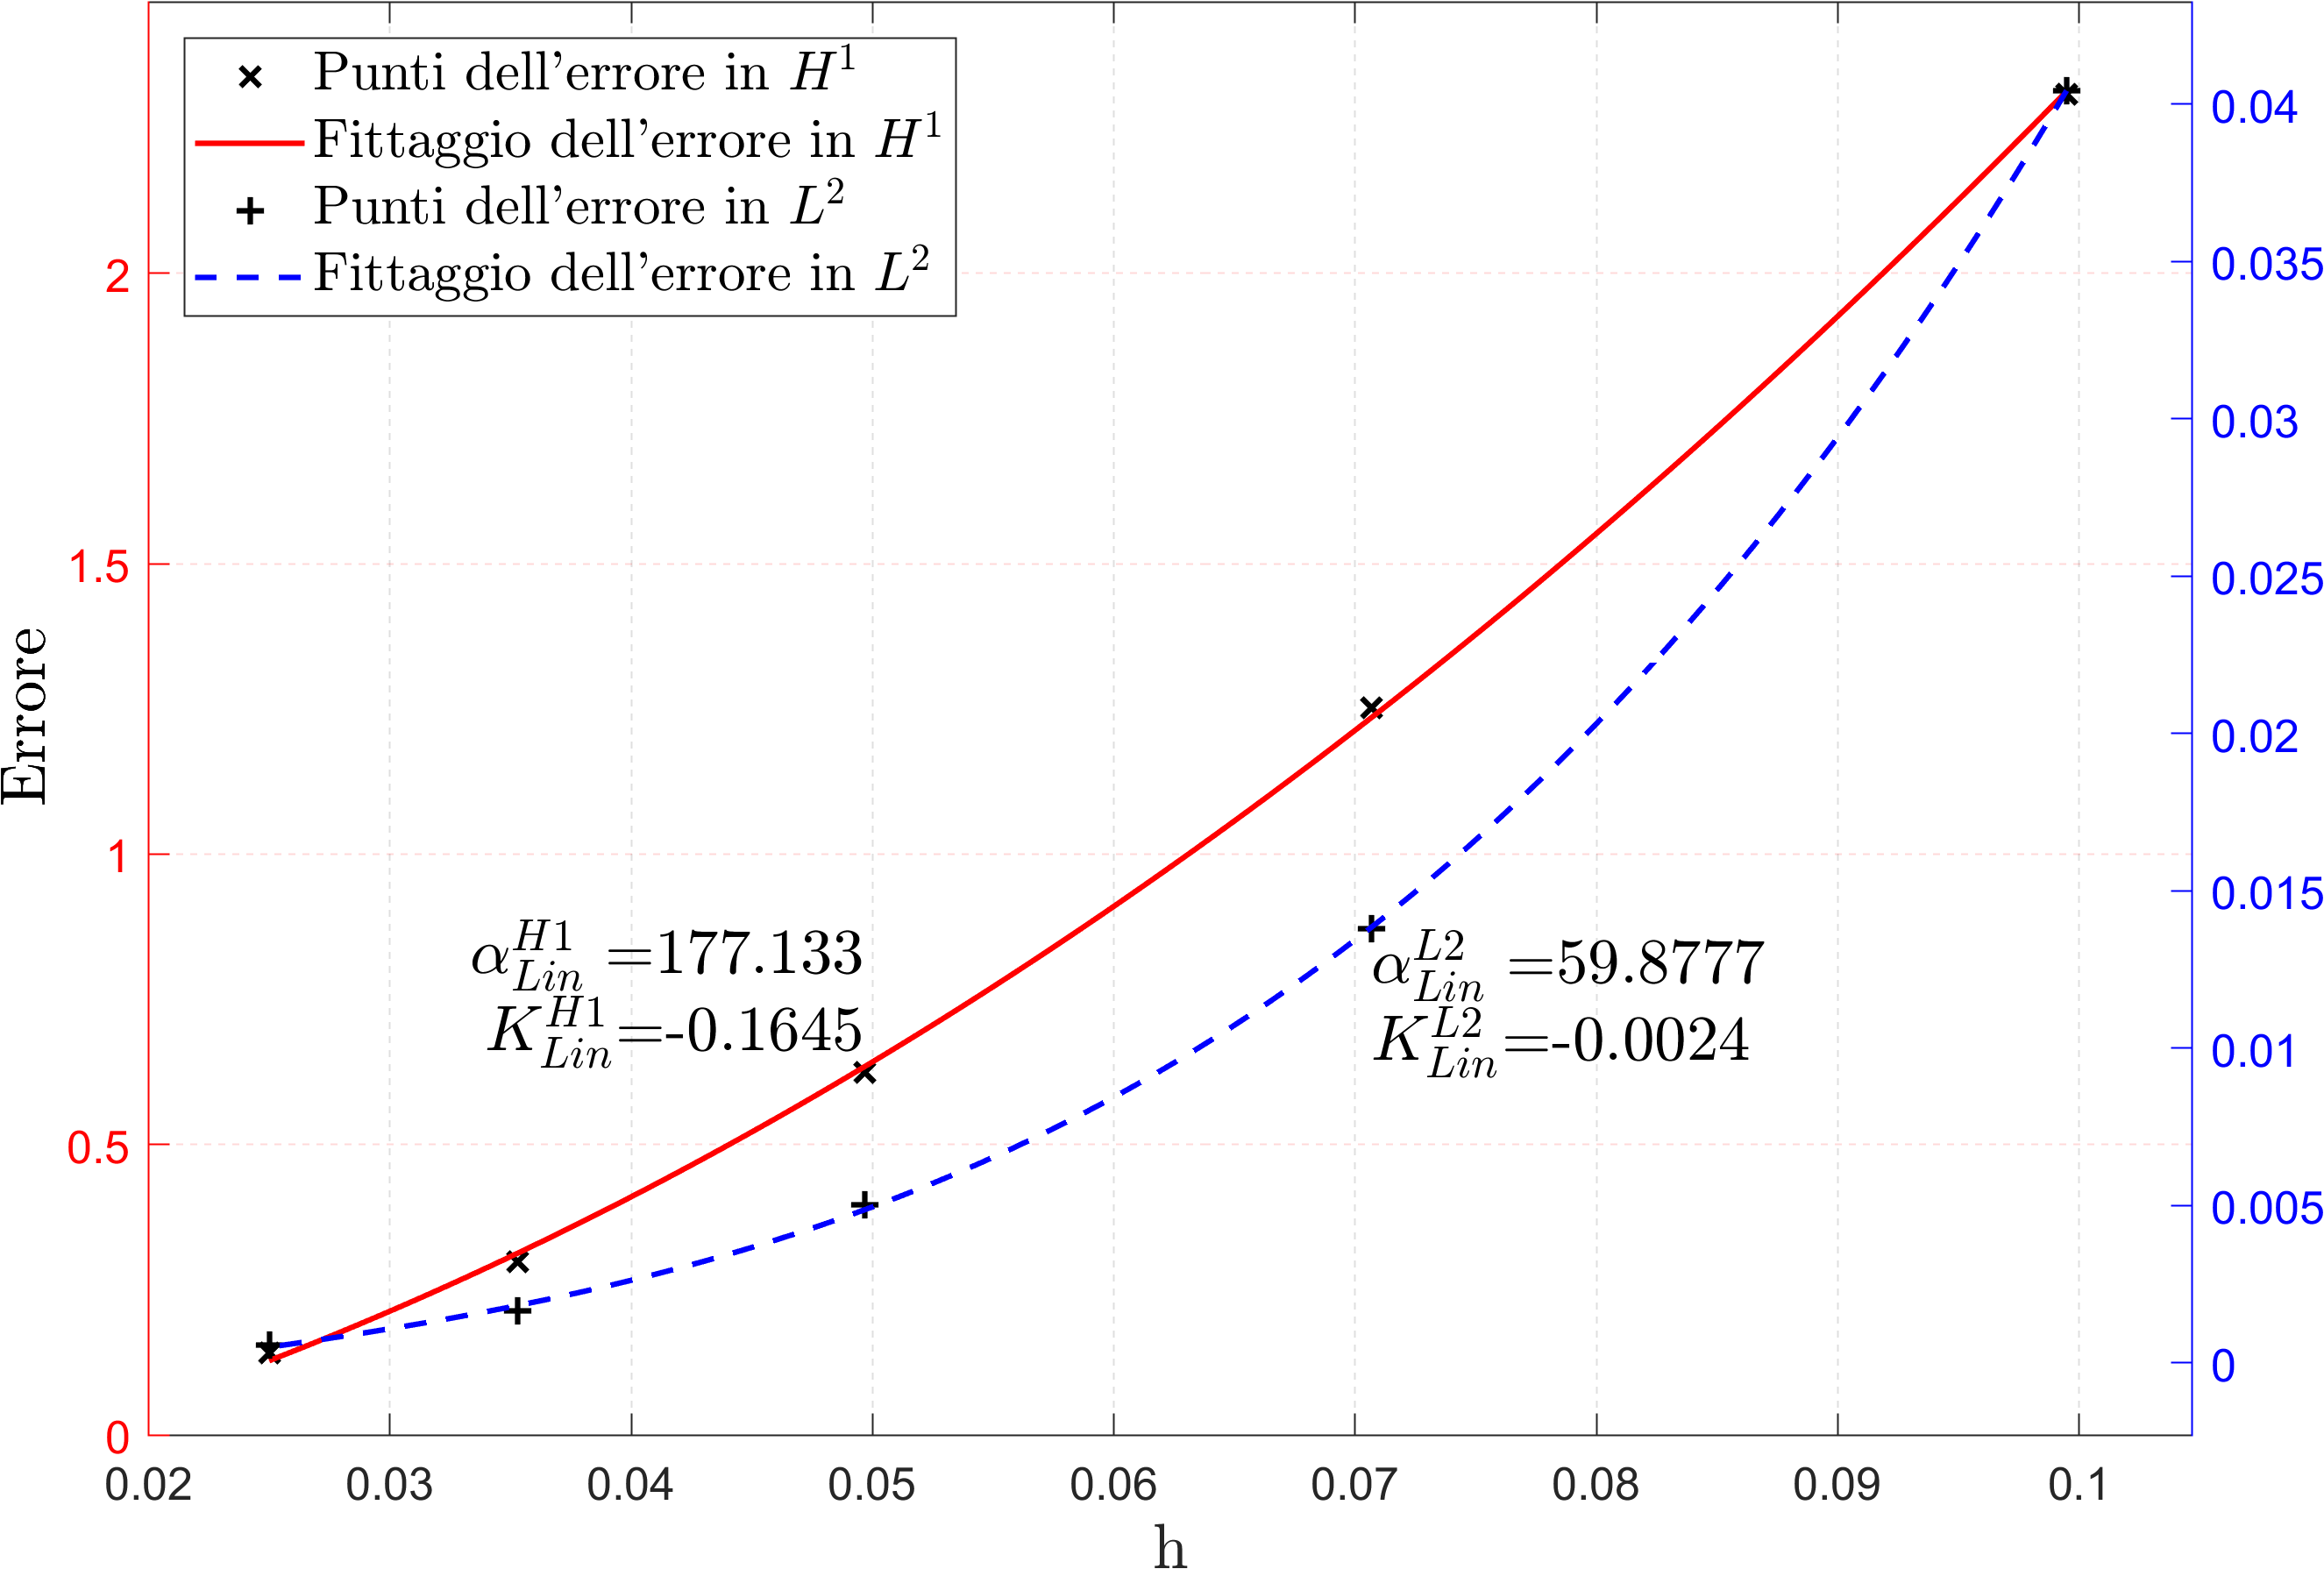
\includegraphics[width=\dimIm]{../Immagini/SDC1_P2_CS_ErrLin_AMax=0.01_NSim=5.png}
                        \caption{Errore dei $\mathbb{P}_2$ in scala lineare con \textit{SUPG}.}
                        \label{figSDC1ErroreP2Lin}
                        \end{subfigure}
                        \distC
                        \begin{subfigure}[t]{\lungSF}
                            \centering
                            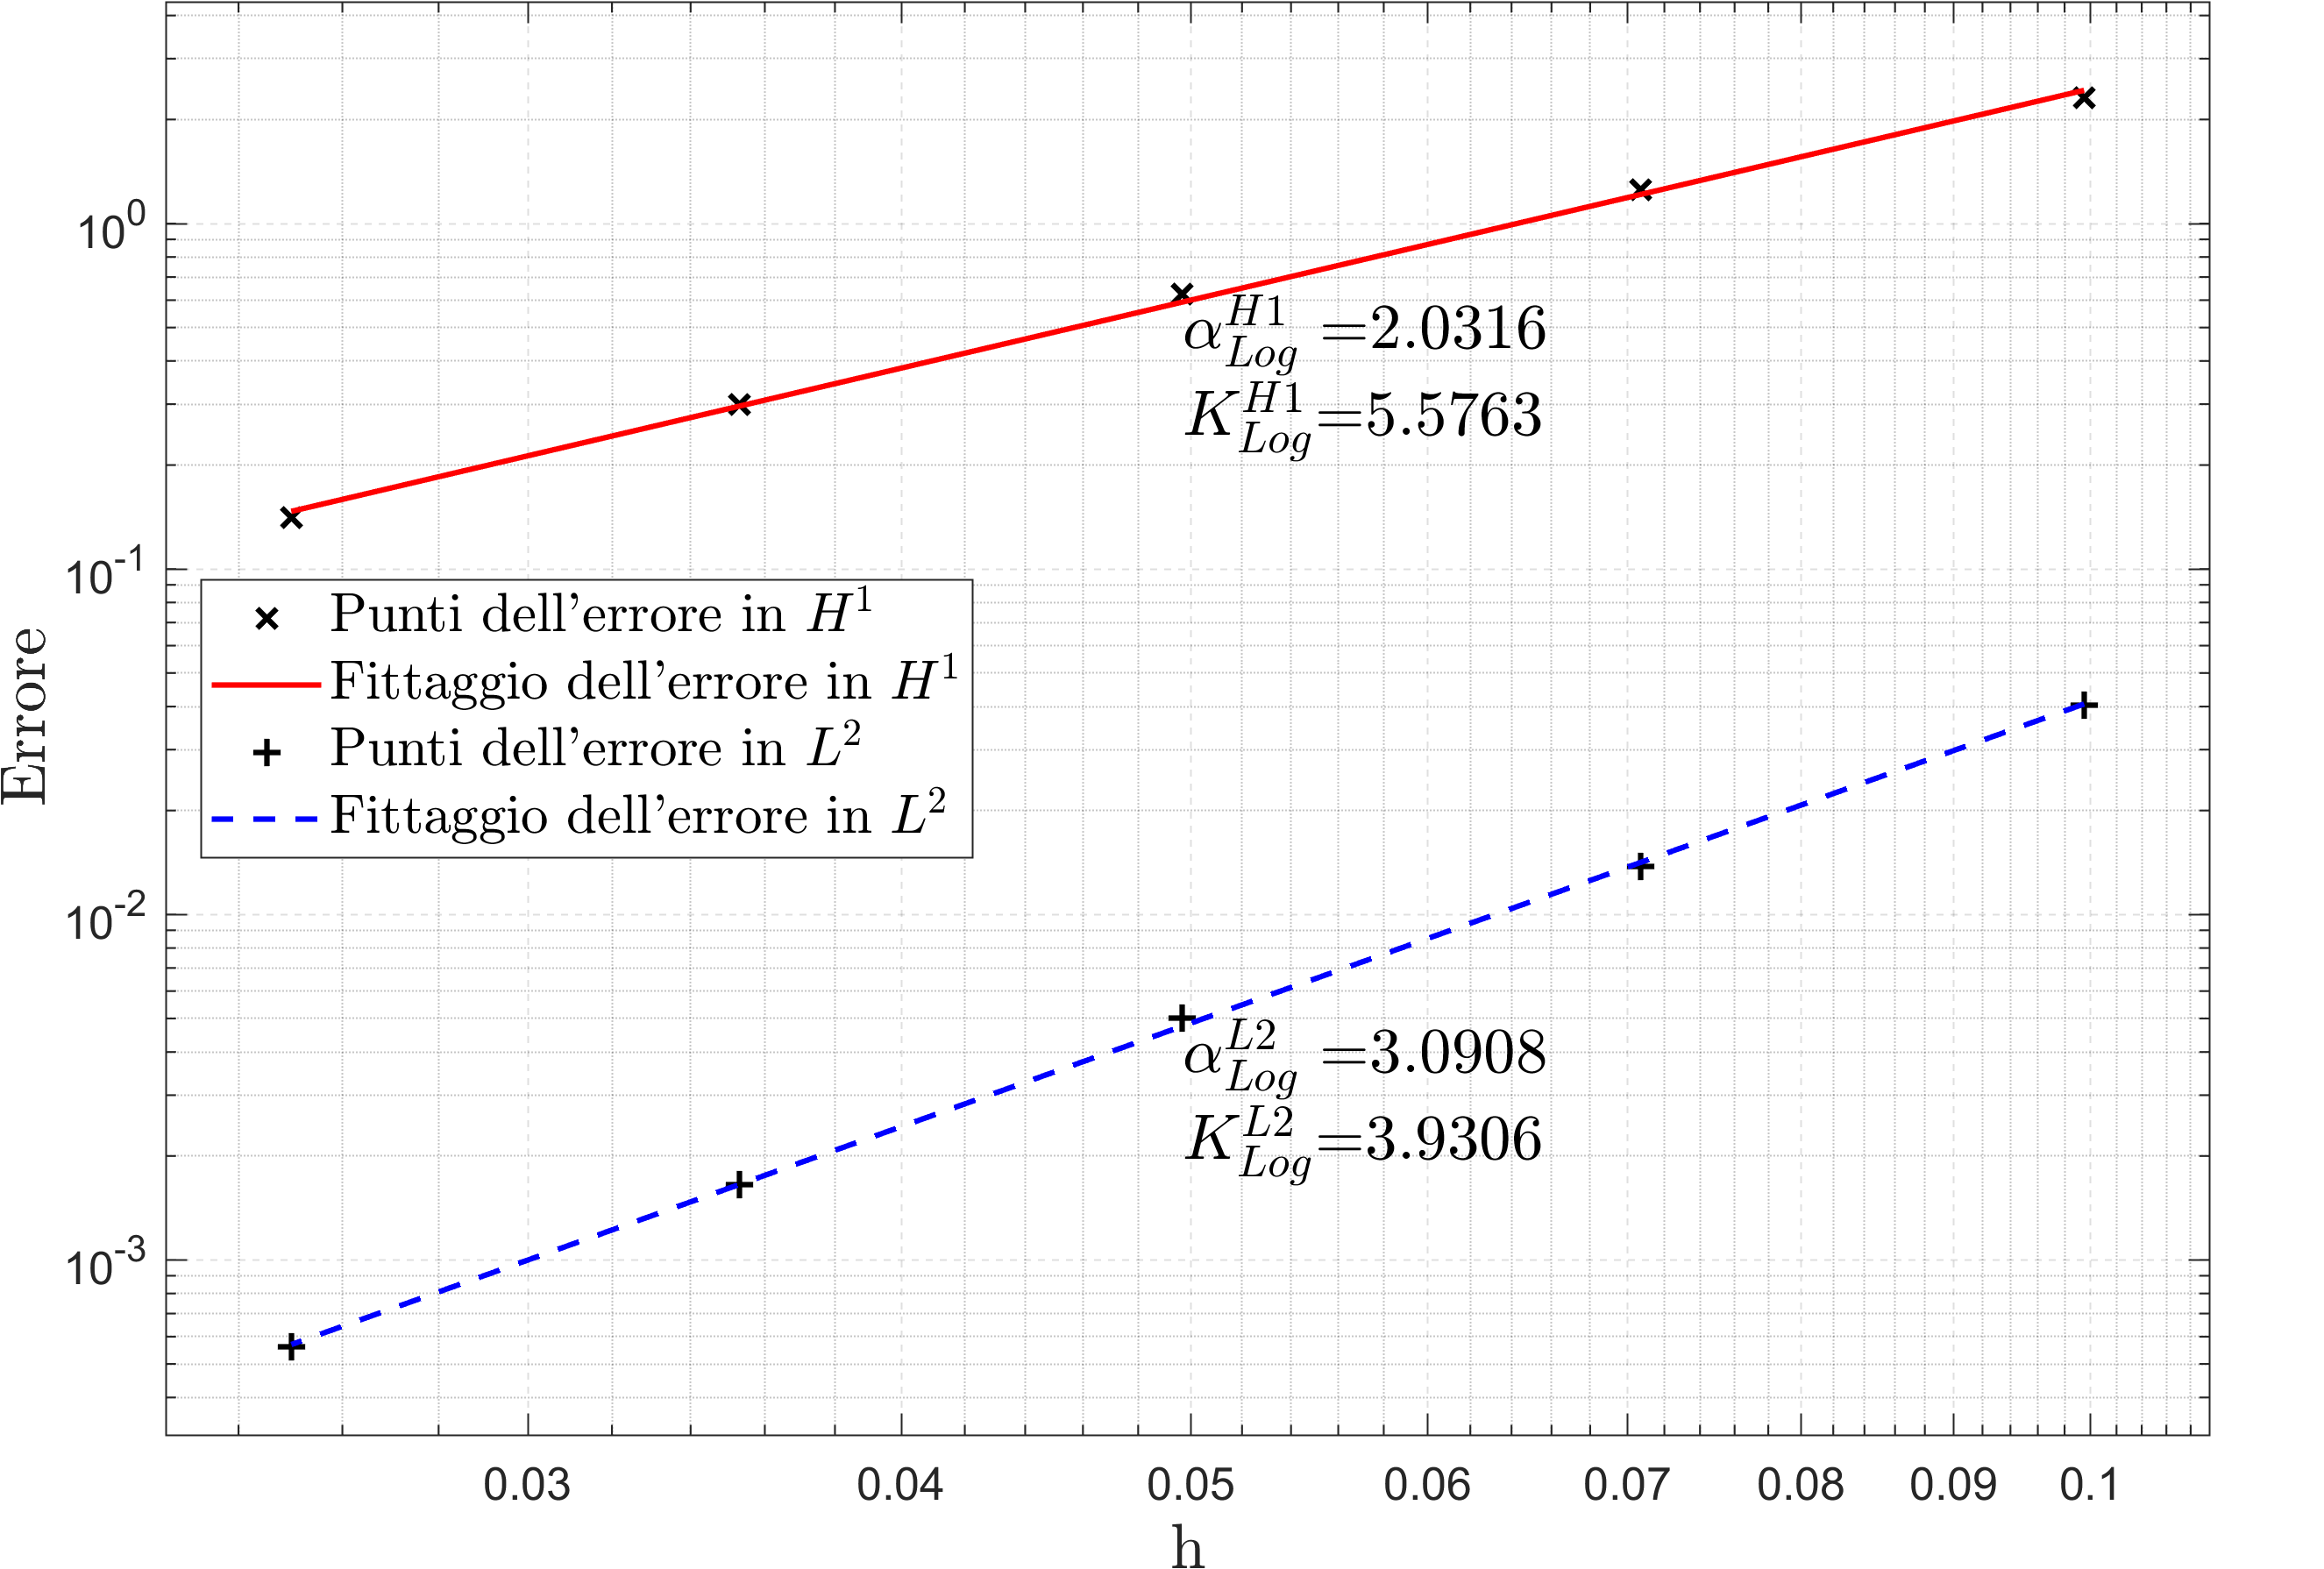
\includegraphics[width=\dimIm]{../Immagini/SDC1_P2_CS_ErrLog_AMax=0.01_NSim=5.png}
                        \caption{Errore dei $\mathbb{P}_2$ in scala logaritmica con \textit{SUPG}.}
                        \label{figSDC1ErroreP2Log}
                        \end{subfigure}
                    }
                    \caption{Nelle Figg. \ref{figSDC1TriangolazioniEsatta}-\ref{figSDC1TriangolazioniApprossimataP2} sono mostrate le soluzioni dell'SDC1: una esatta e le altre approssimate con \textit{SUPG}; invece nelle \ref{figSDC1ErroreP1Lin}-\ref{figSDC1ErroreP2Log} sono illustrati in due scale diverse gli errori in norma $H^1$ ed $L^2$ con \textit{SUPG}. I parametri dati a \textit{BBTR} sono spiegati nel $\S$\ref{parPremessaParametriBBTR}.}
                    \label{figSDC1}
                \end{figure*}

                \begin{figure*}[p]
                    \newcommand{\distR}{\vspace{15pt}} % Distanza tra le righe
                    
                    \newcommand{\lungSF}{0.33\textwidth}
                    \newcommand{\dimIm}{4cm}
                    \makebox[\linewidth][c]{
                        \begin{subfigure}[t]{\lungSF}
                            \centering
                            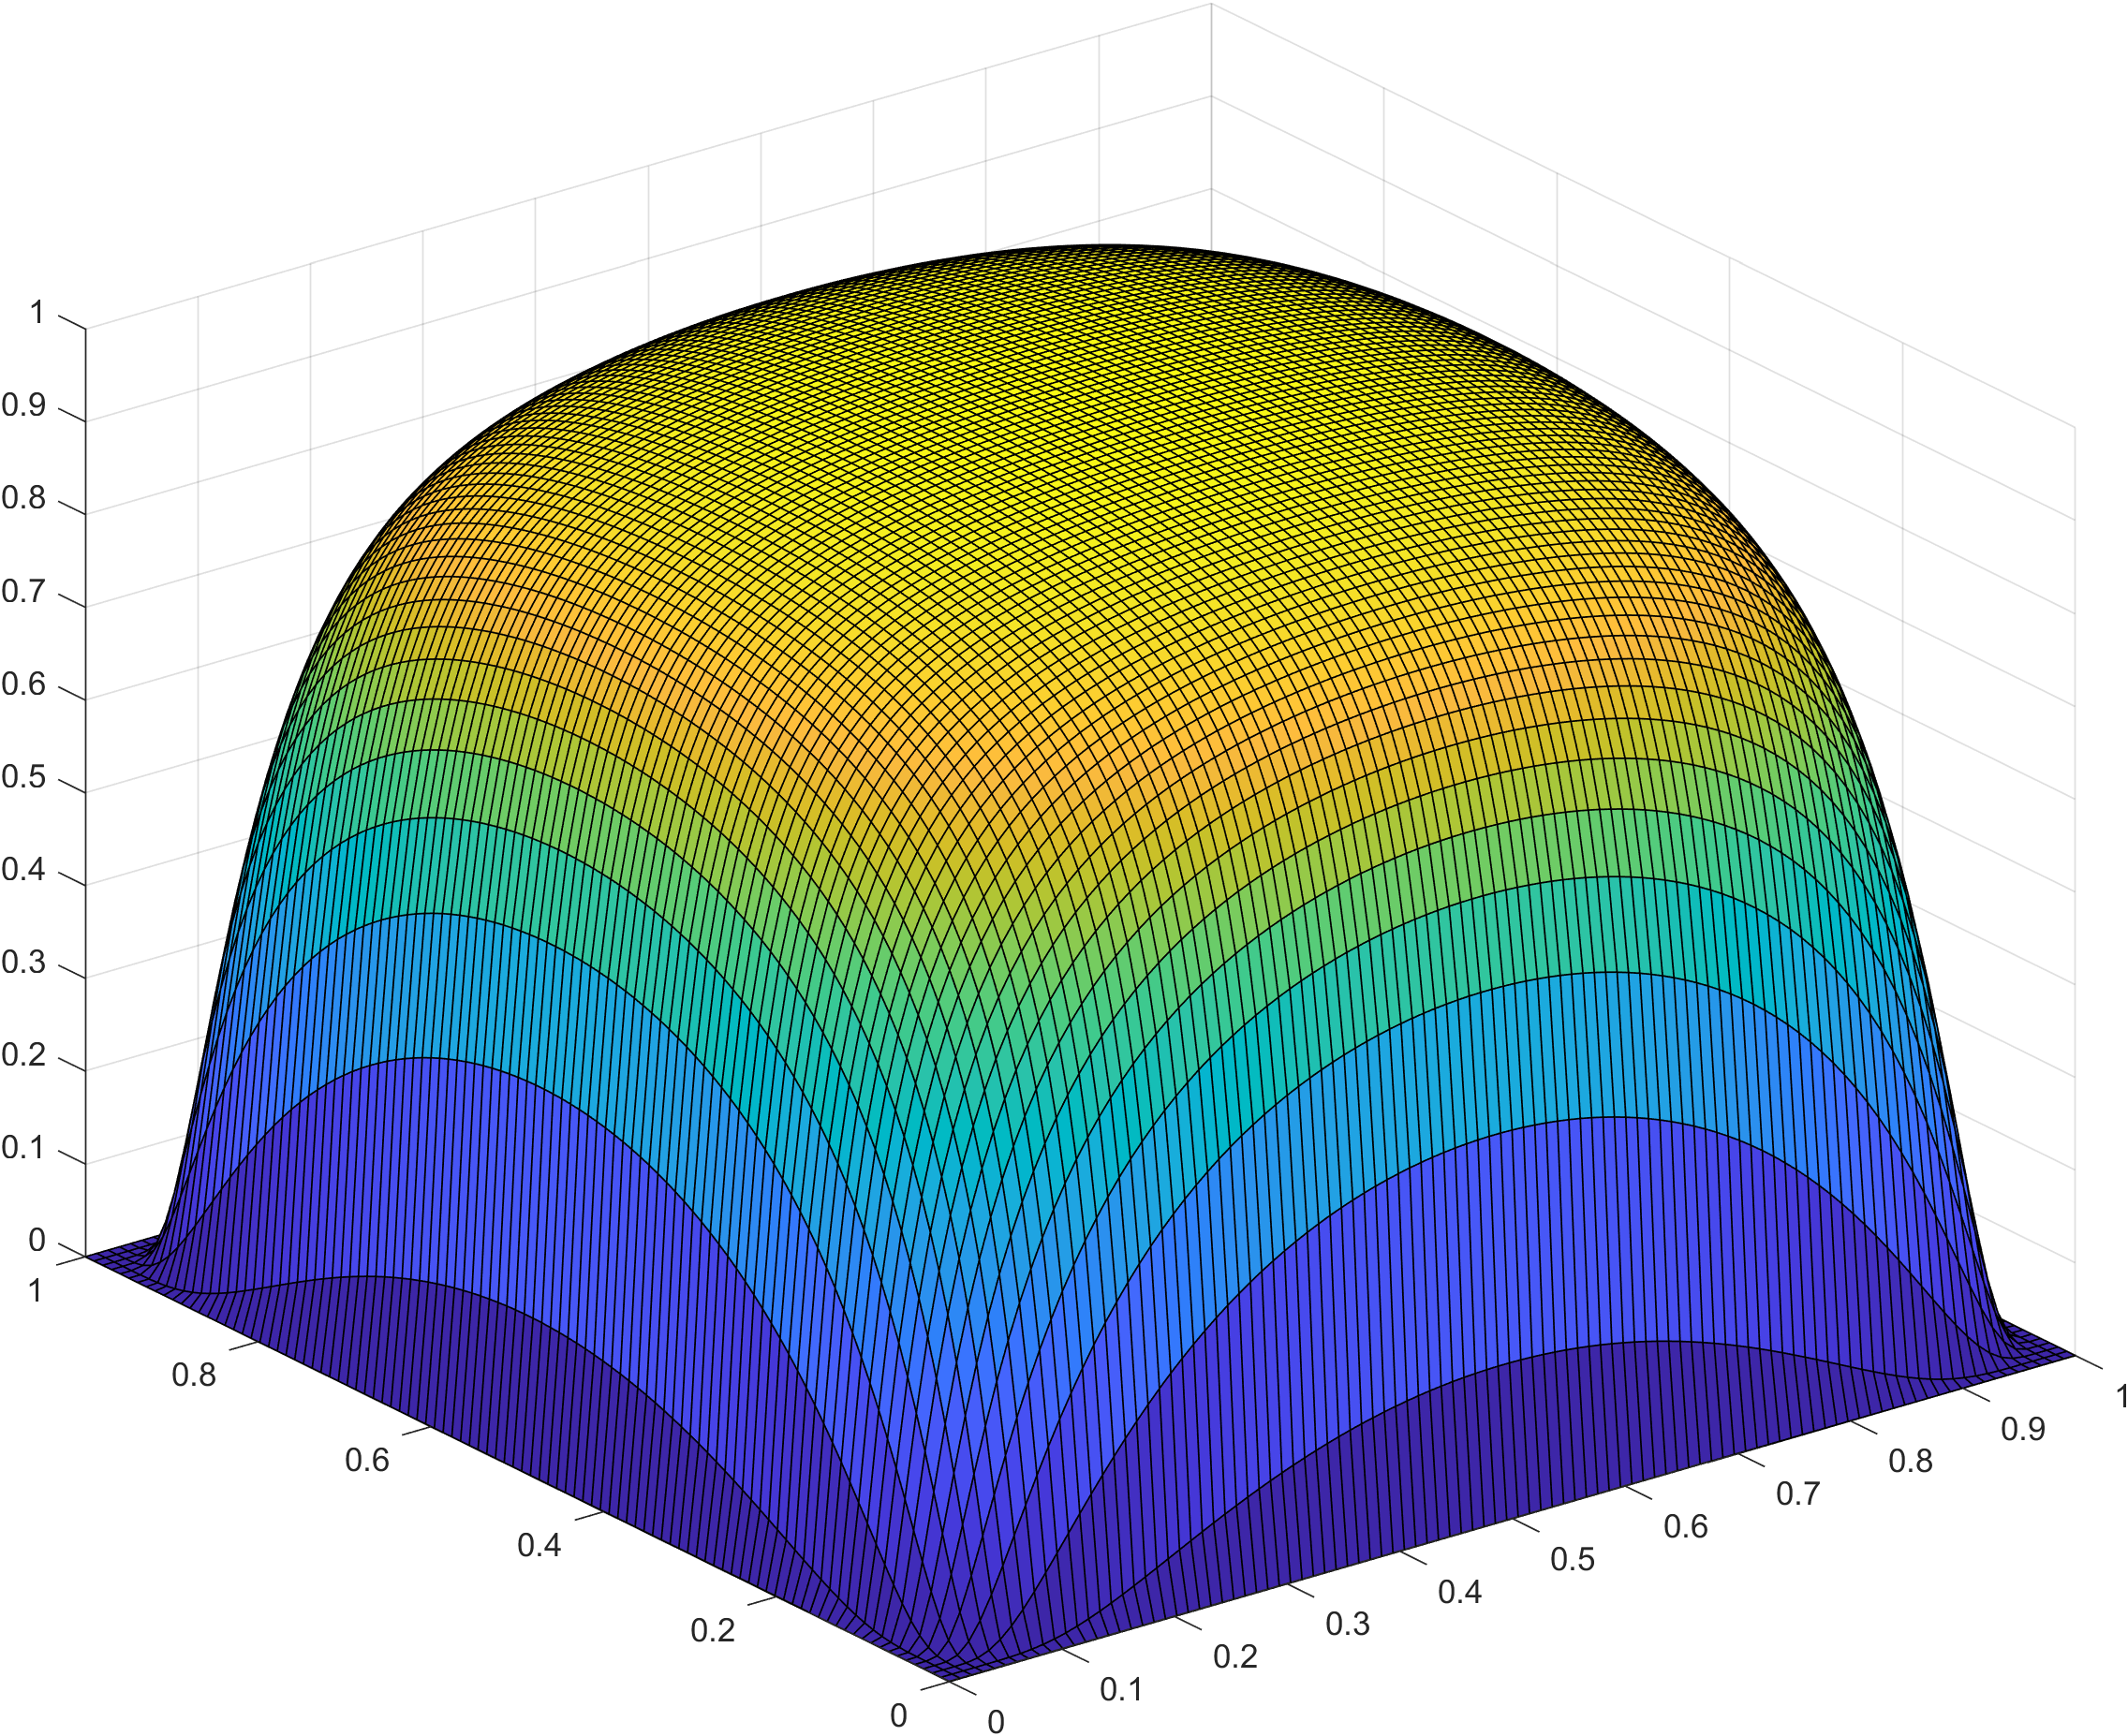
\includegraphics[height=\dimIm]{../Immagini/SDC2_SDR2_SE_NPunti=100.png}
                            \caption{Soluzione esatta.}
                            \label{figSDC2TriangolazioniEsatta}
                        \end{subfigure}
                        \begin{subfigure}[t]{\lungSF}
                            \centering
                            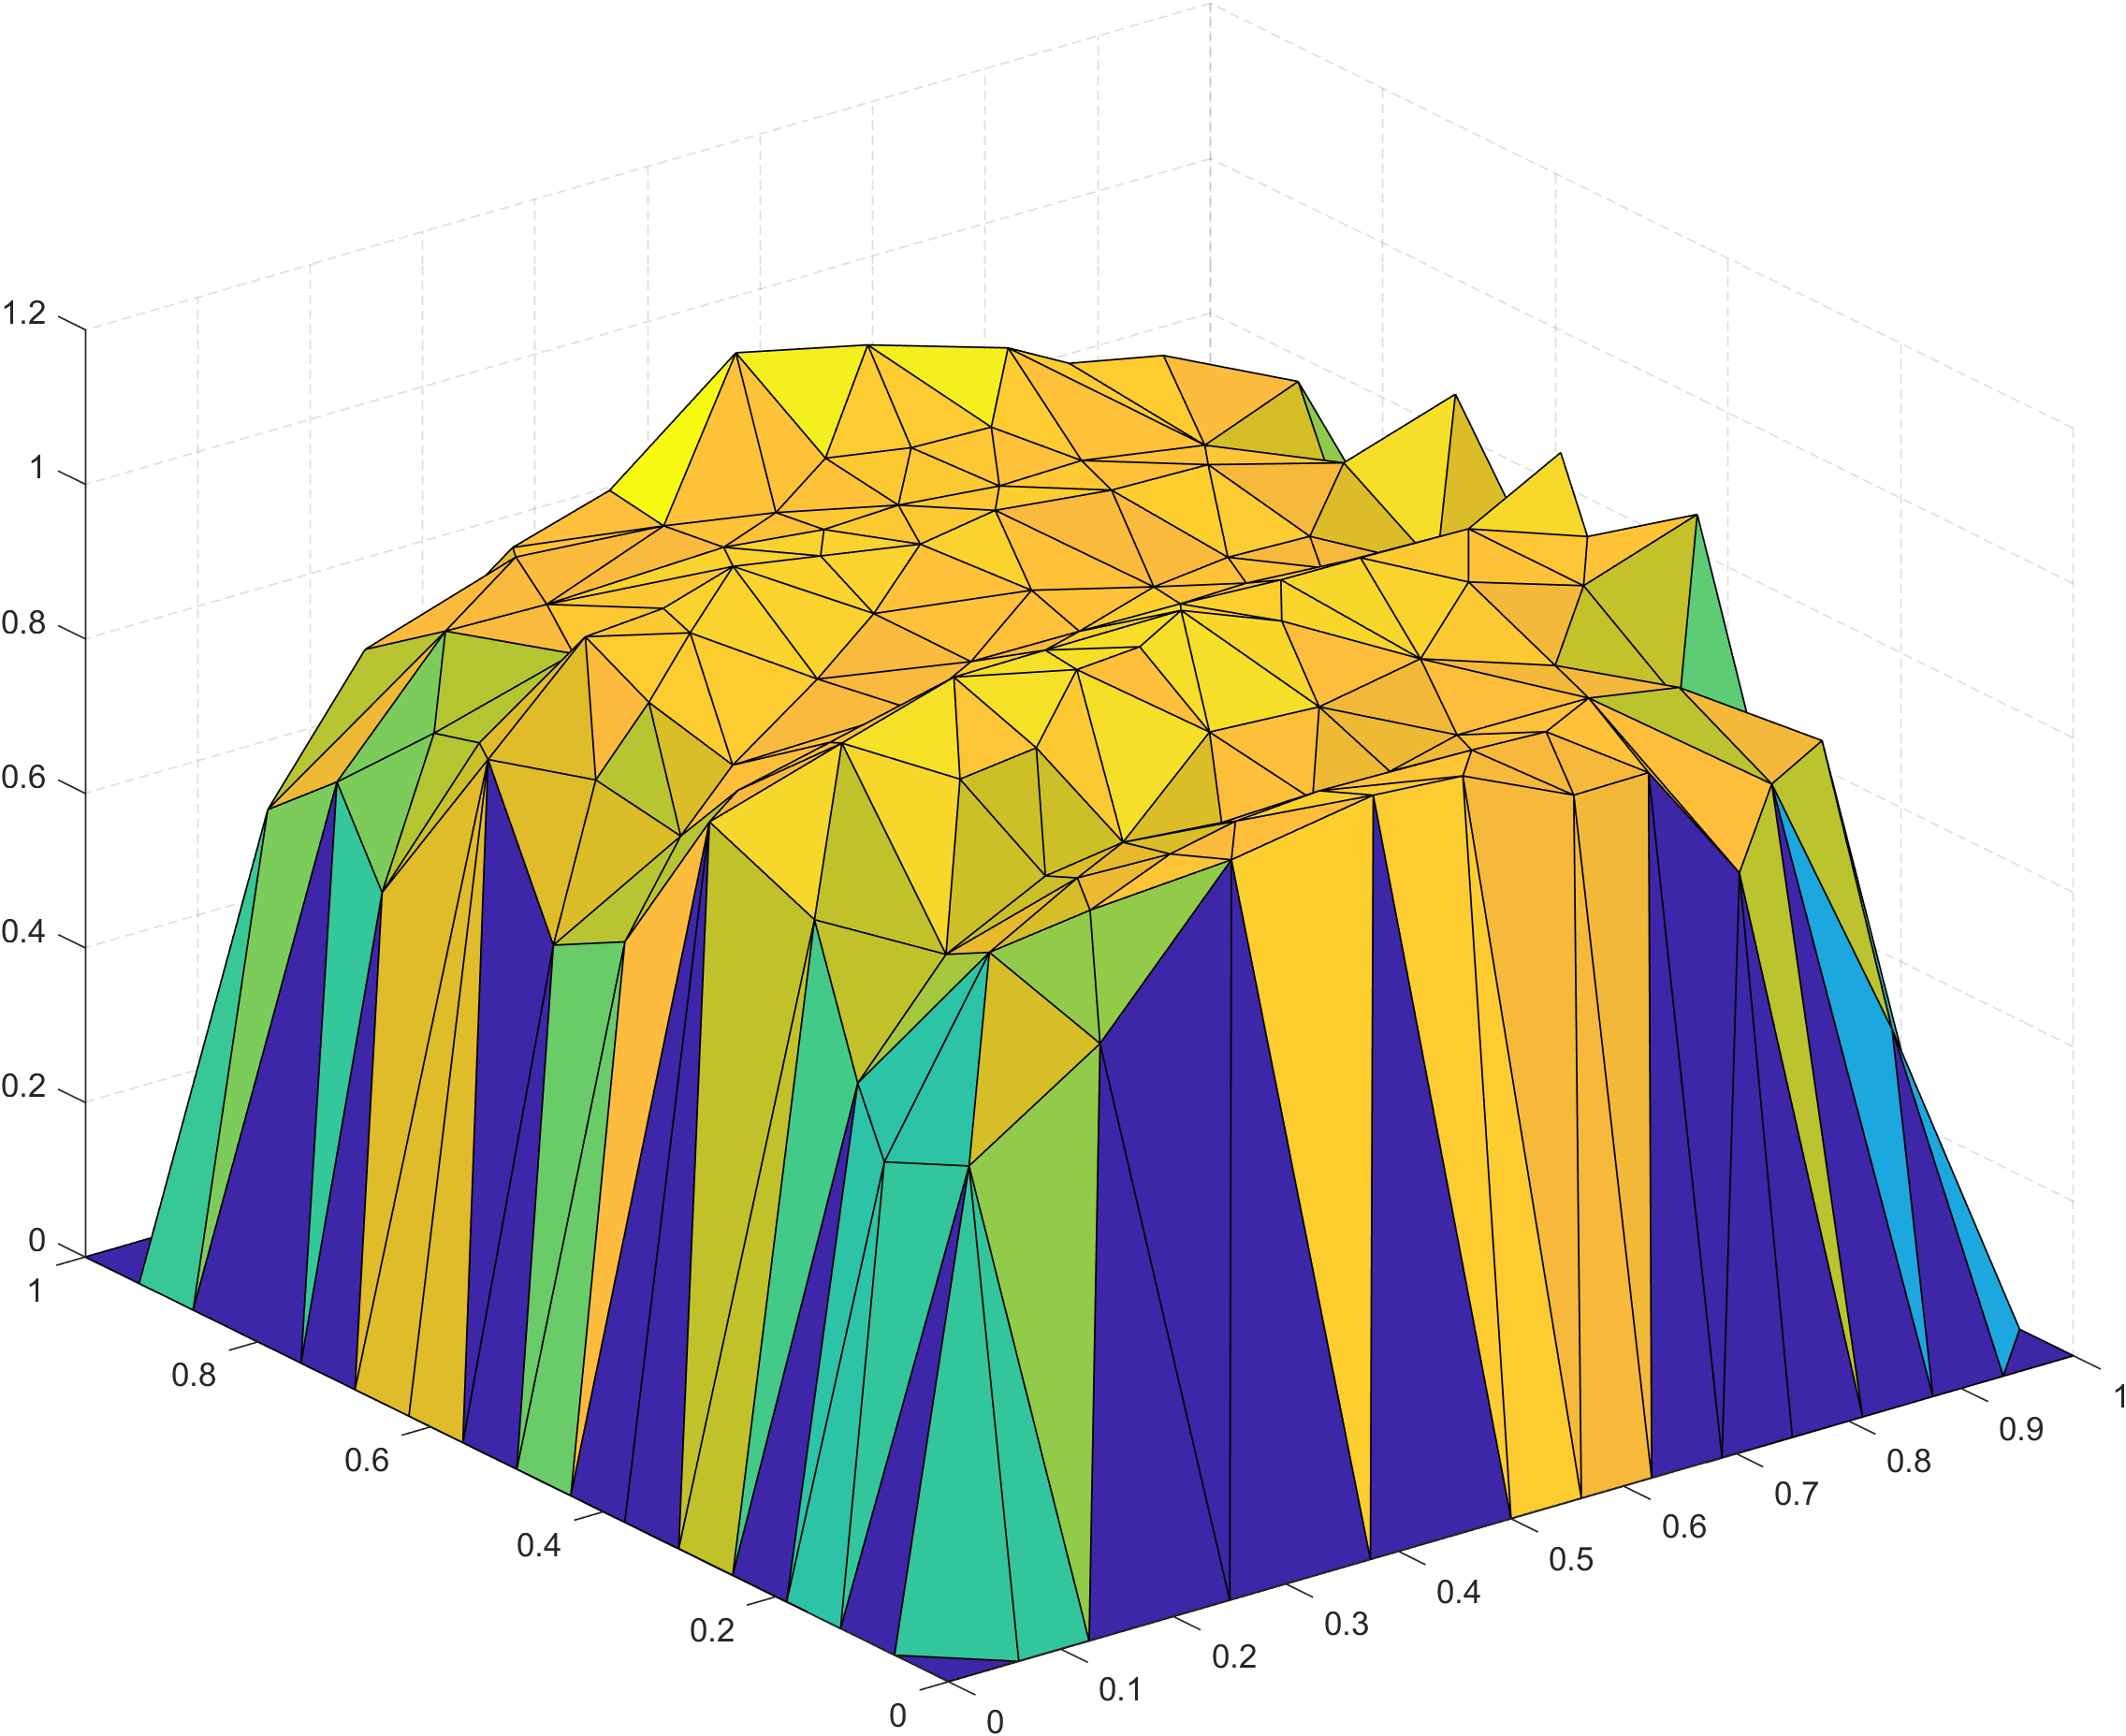
\includegraphics[height=\dimIm]{../Immagini/SDC2_CS_P1_AMax=0.005.png}
                            \caption{Soluzione qualitativa coi $\mathbb{P}_1$ ed \textit{SUPG}.}
                            \label{figSDC2TriangolazioniApprossimataP1}
                        \end{subfigure}
                        \begin{subfigure}[t]{\lungSF}
                            \centering
                            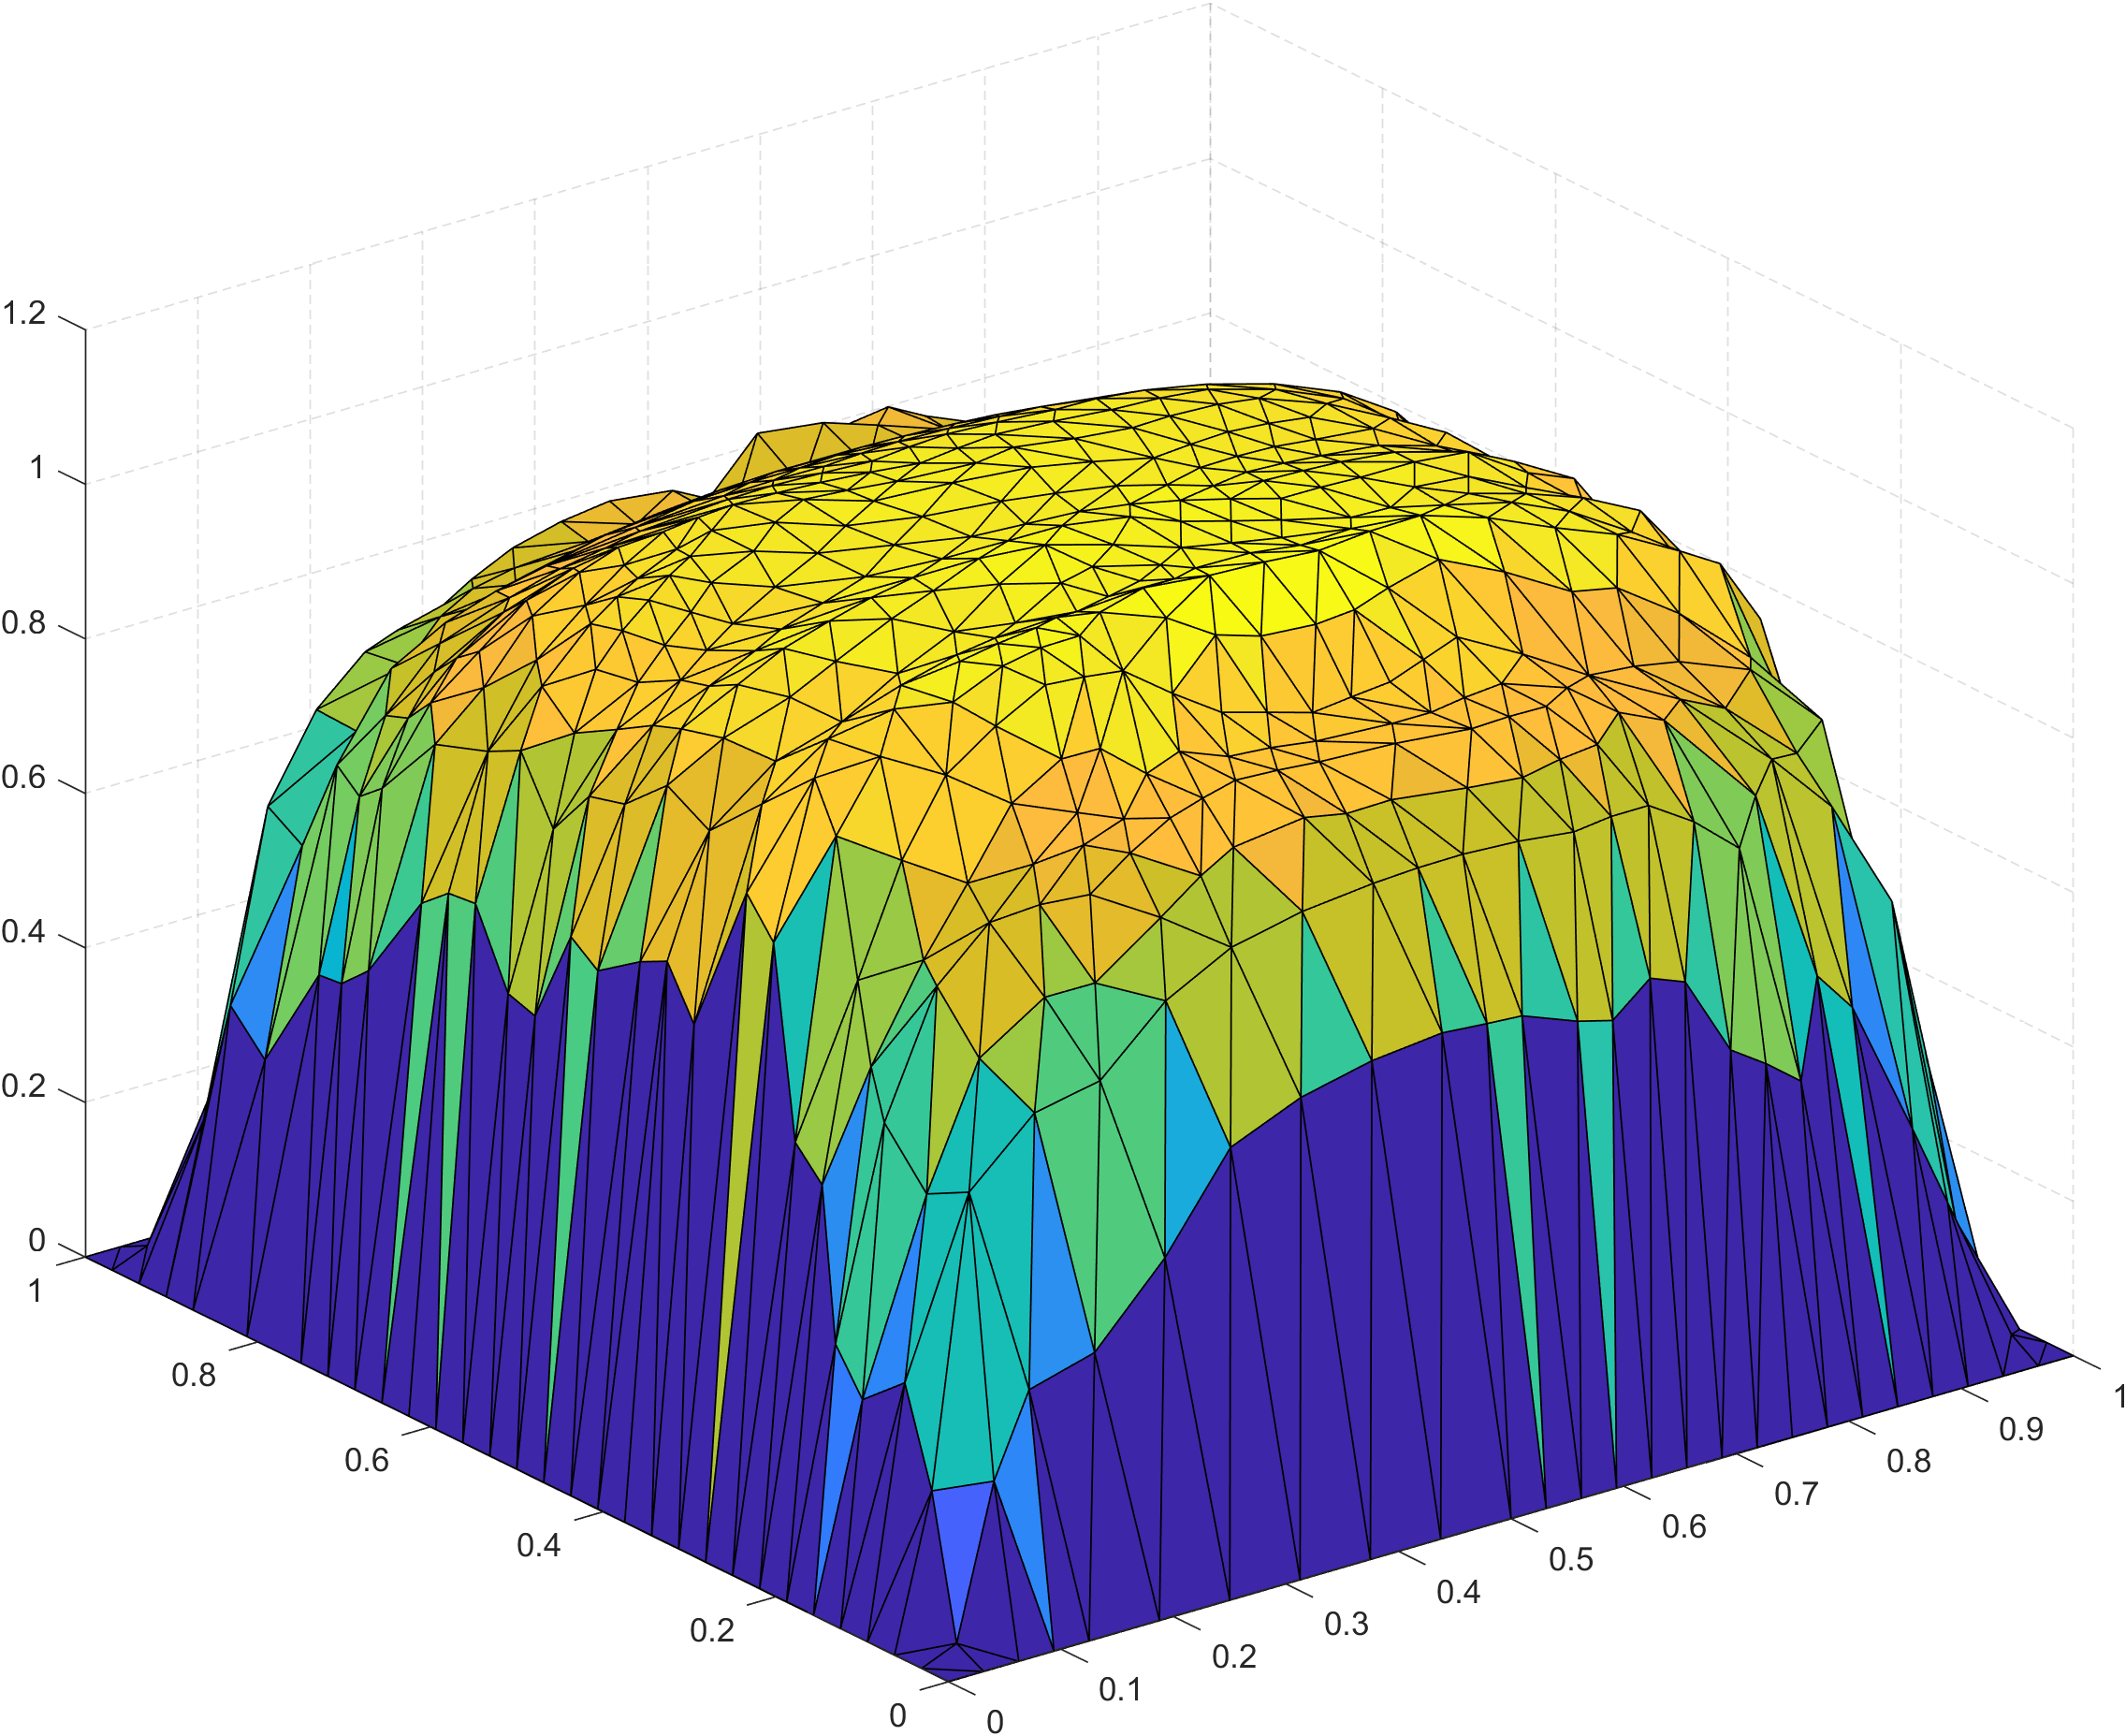
\includegraphics[height=\dimIm]{../Immagini/SDC2_CS_P2_AMax=0.005.png}
                            \caption{Soluzione qualitativa coi $\mathbb{P}_2$ ed \textit{SUPG}.}
                            \label{figSDC2TriangolazioniApprossimataP2}
                        \end{subfigure}
                    }
                    \distR
        
                    \renewcommand{\lungSF}{.5\linewidth}
                    \renewcommand{\dimIm}{\linewidth}
                    \newcommand{\distC}{\hspace{7.5pt}} % Distanza tra le colonne
                    \makebox[\linewidth][c]{
                        \begin{subfigure}[t]{\lungSF}
                            \centering
                            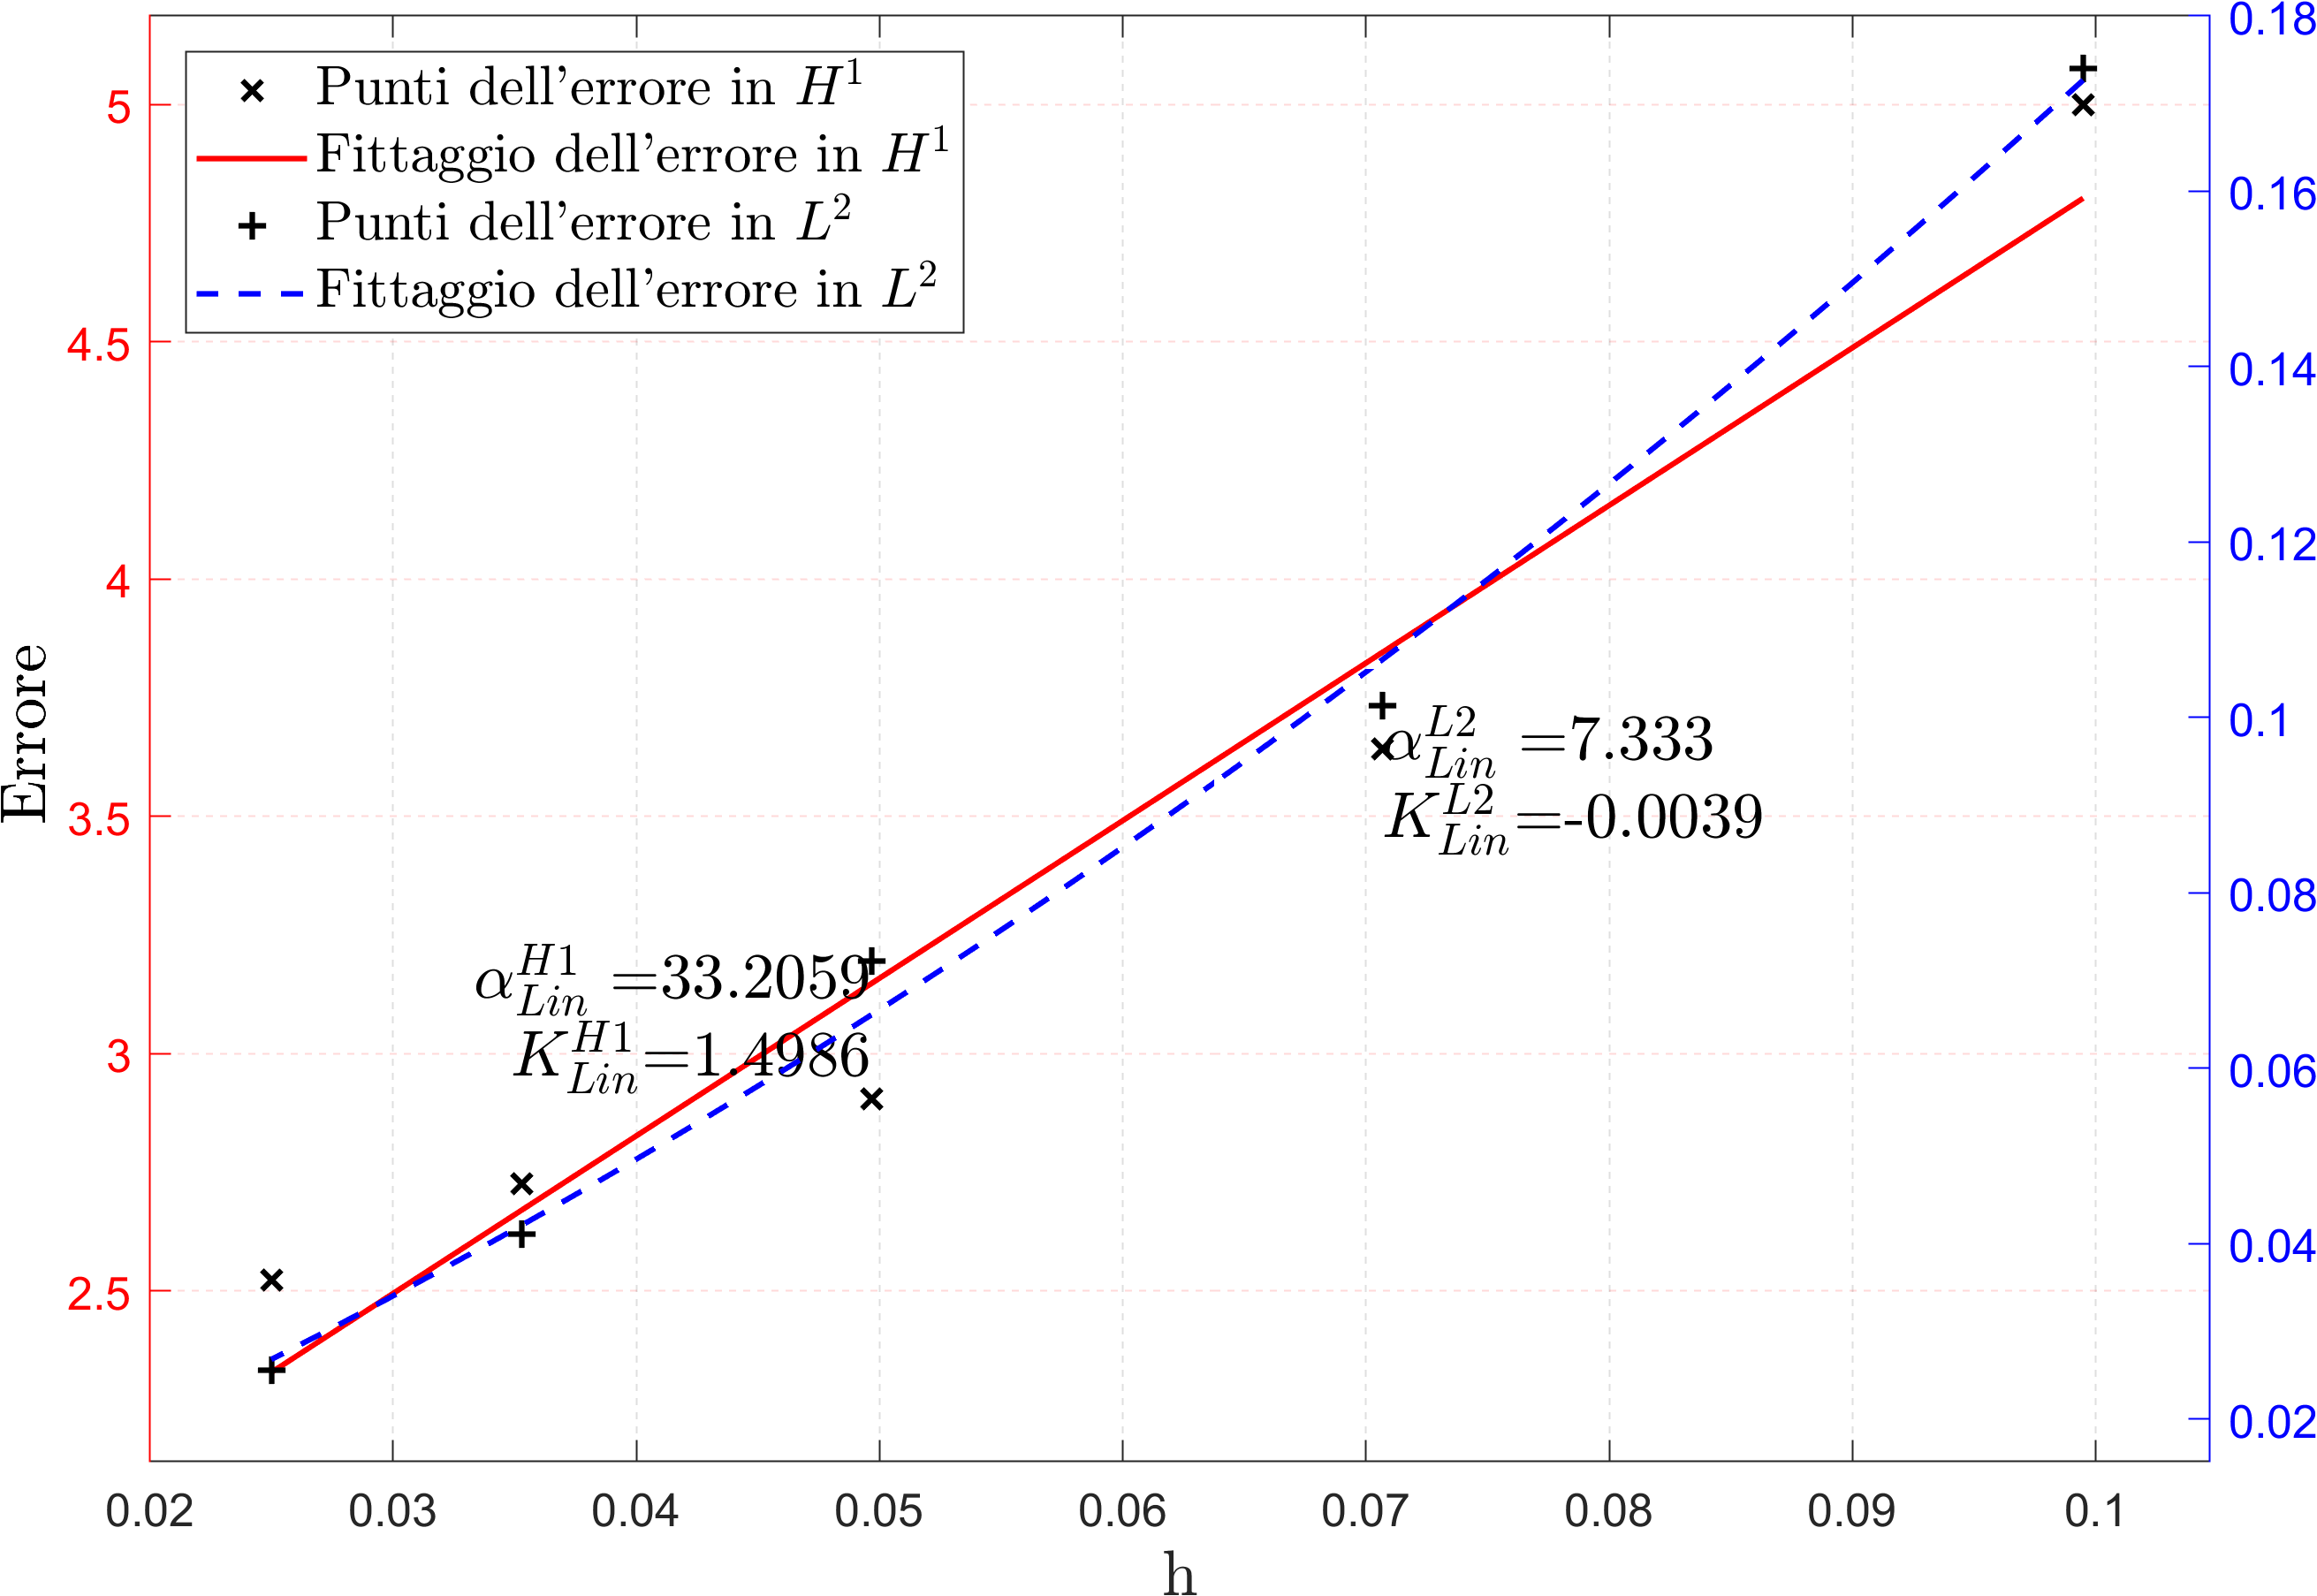
\includegraphics[width=\dimIm]{../Immagini/SDC2_P1_CS_ErrLin_AMax=0.01_NSim=5.png}
                            \caption{Errore dei $\mathbb{P}_1$ in scala lineare con \textit{SUPG}.}
                            \label{figSDC2ErroreP1Lin}
                        \end{subfigure}
                        \distC
                        \begin{subfigure}[t]{\lungSF}
                            \centering
                            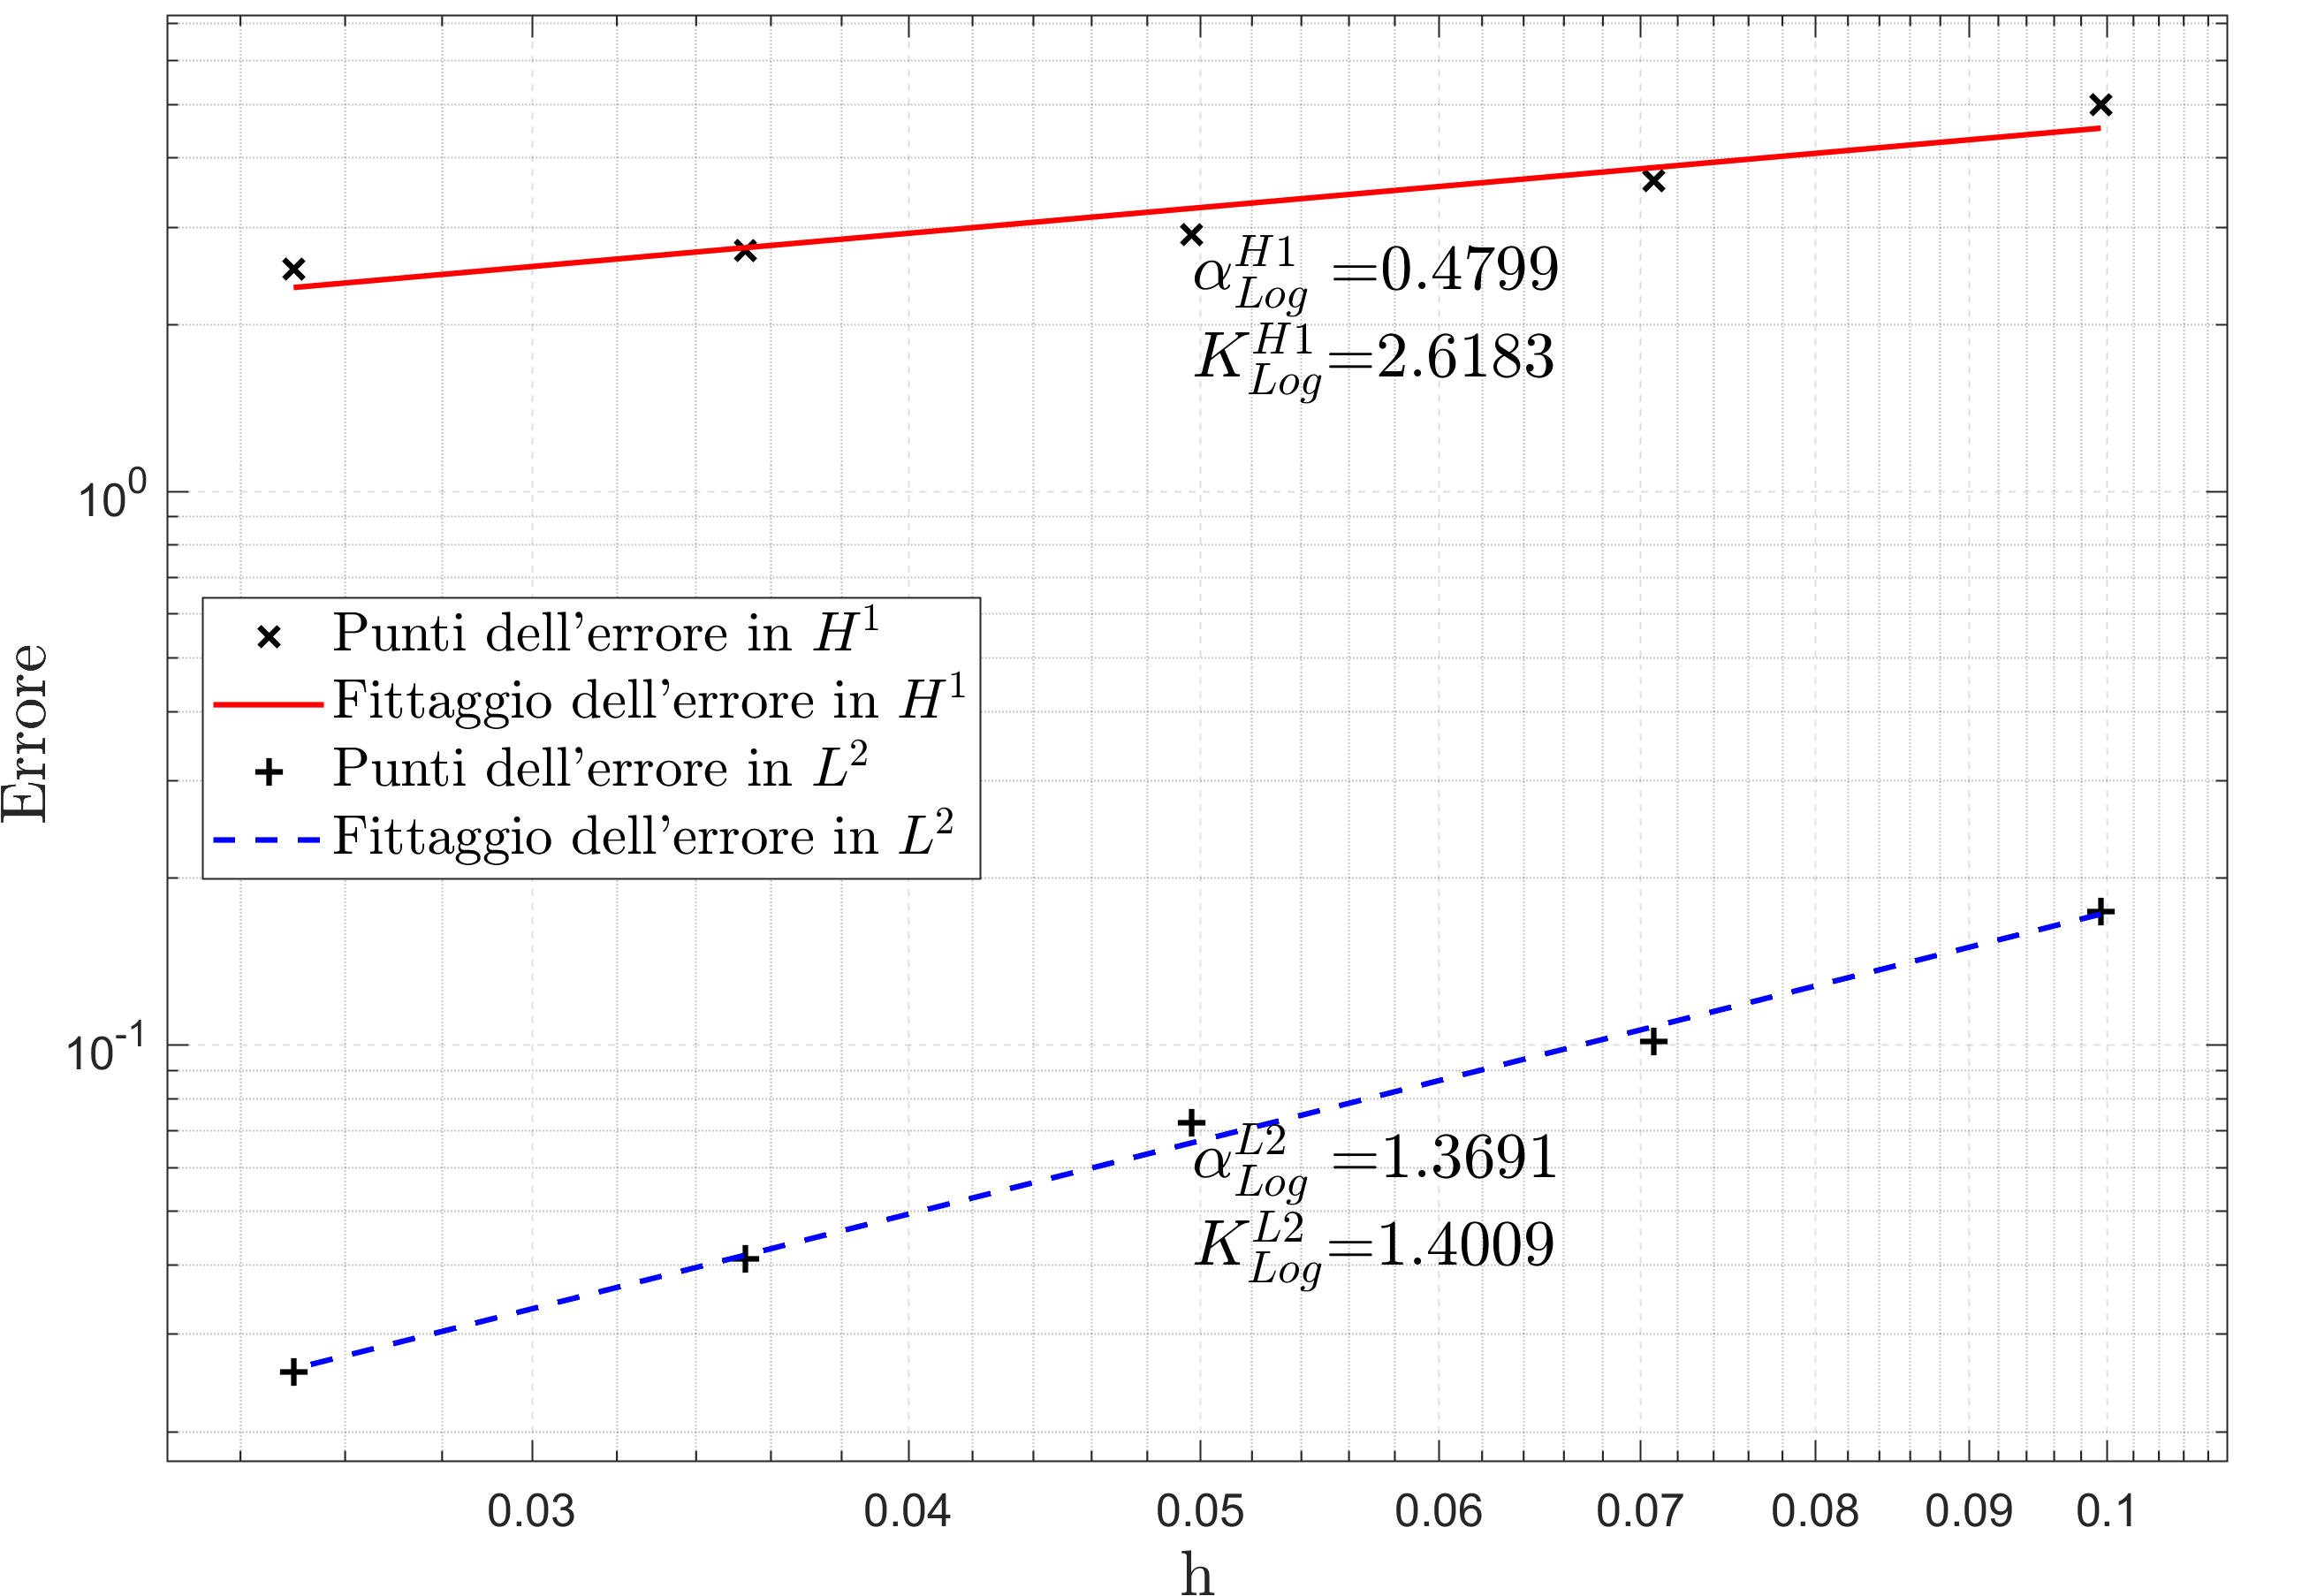
\includegraphics[width=\dimIm]{../Immagini/SDC2_P1_CS_ErrLog_AMax=0.01_NSim=5.png}
                            \caption{Errore dei $\mathbb{P}_1$ in scala logaritmica con \textit{SUPG}.}
                            \label{figSDC2ErroreP1Log}
                        \end{subfigure}
                    }
                    \distR
        
                    \makebox[\linewidth][c]{
                        \begin{subfigure}[t]{\lungSF}
                            \centering
                            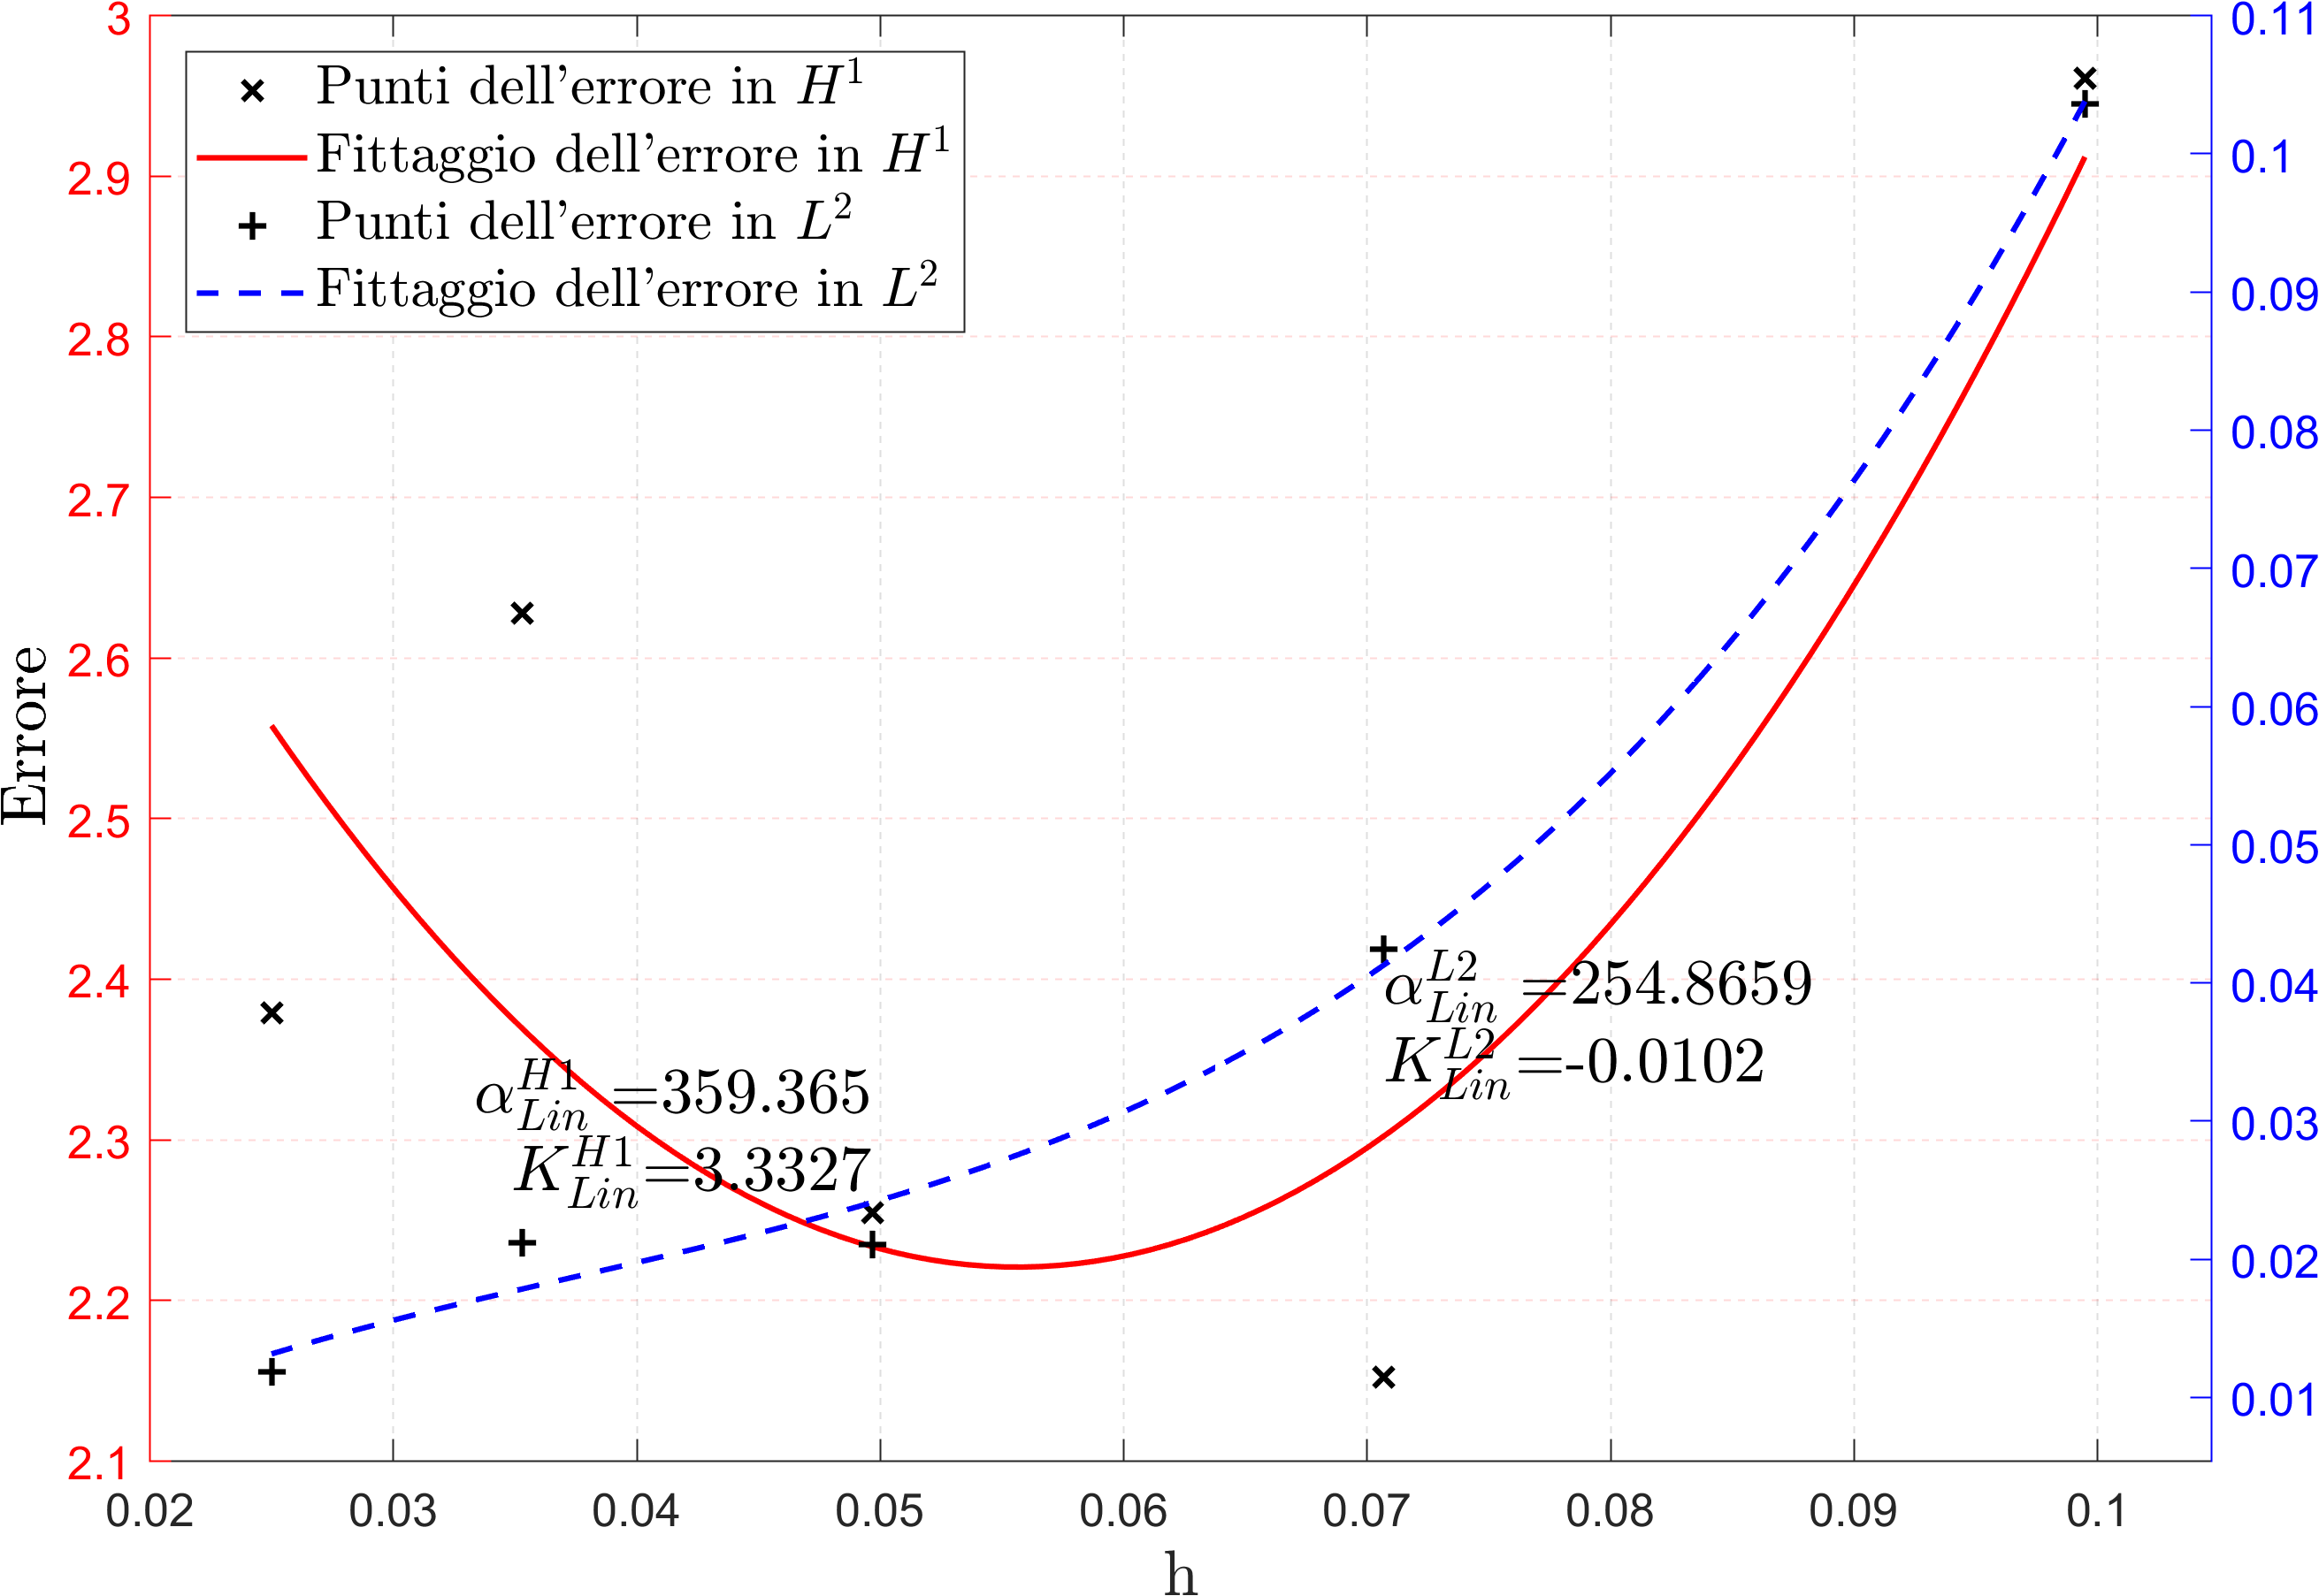
\includegraphics[width=\dimIm]{../Immagini/SDC2_P2_CS_ErrLin_AMax=0.01_NSim=5.png}
                            \caption{Errore dei $\mathbb{P}_2$ in scala lineare con \textit{SUPG}.}
                            \label{figSDC2ErroreP2Lin}
                        \end{subfigure}
                        \distC
                        \begin{subfigure}[t]{\lungSF}
                            \centering
                            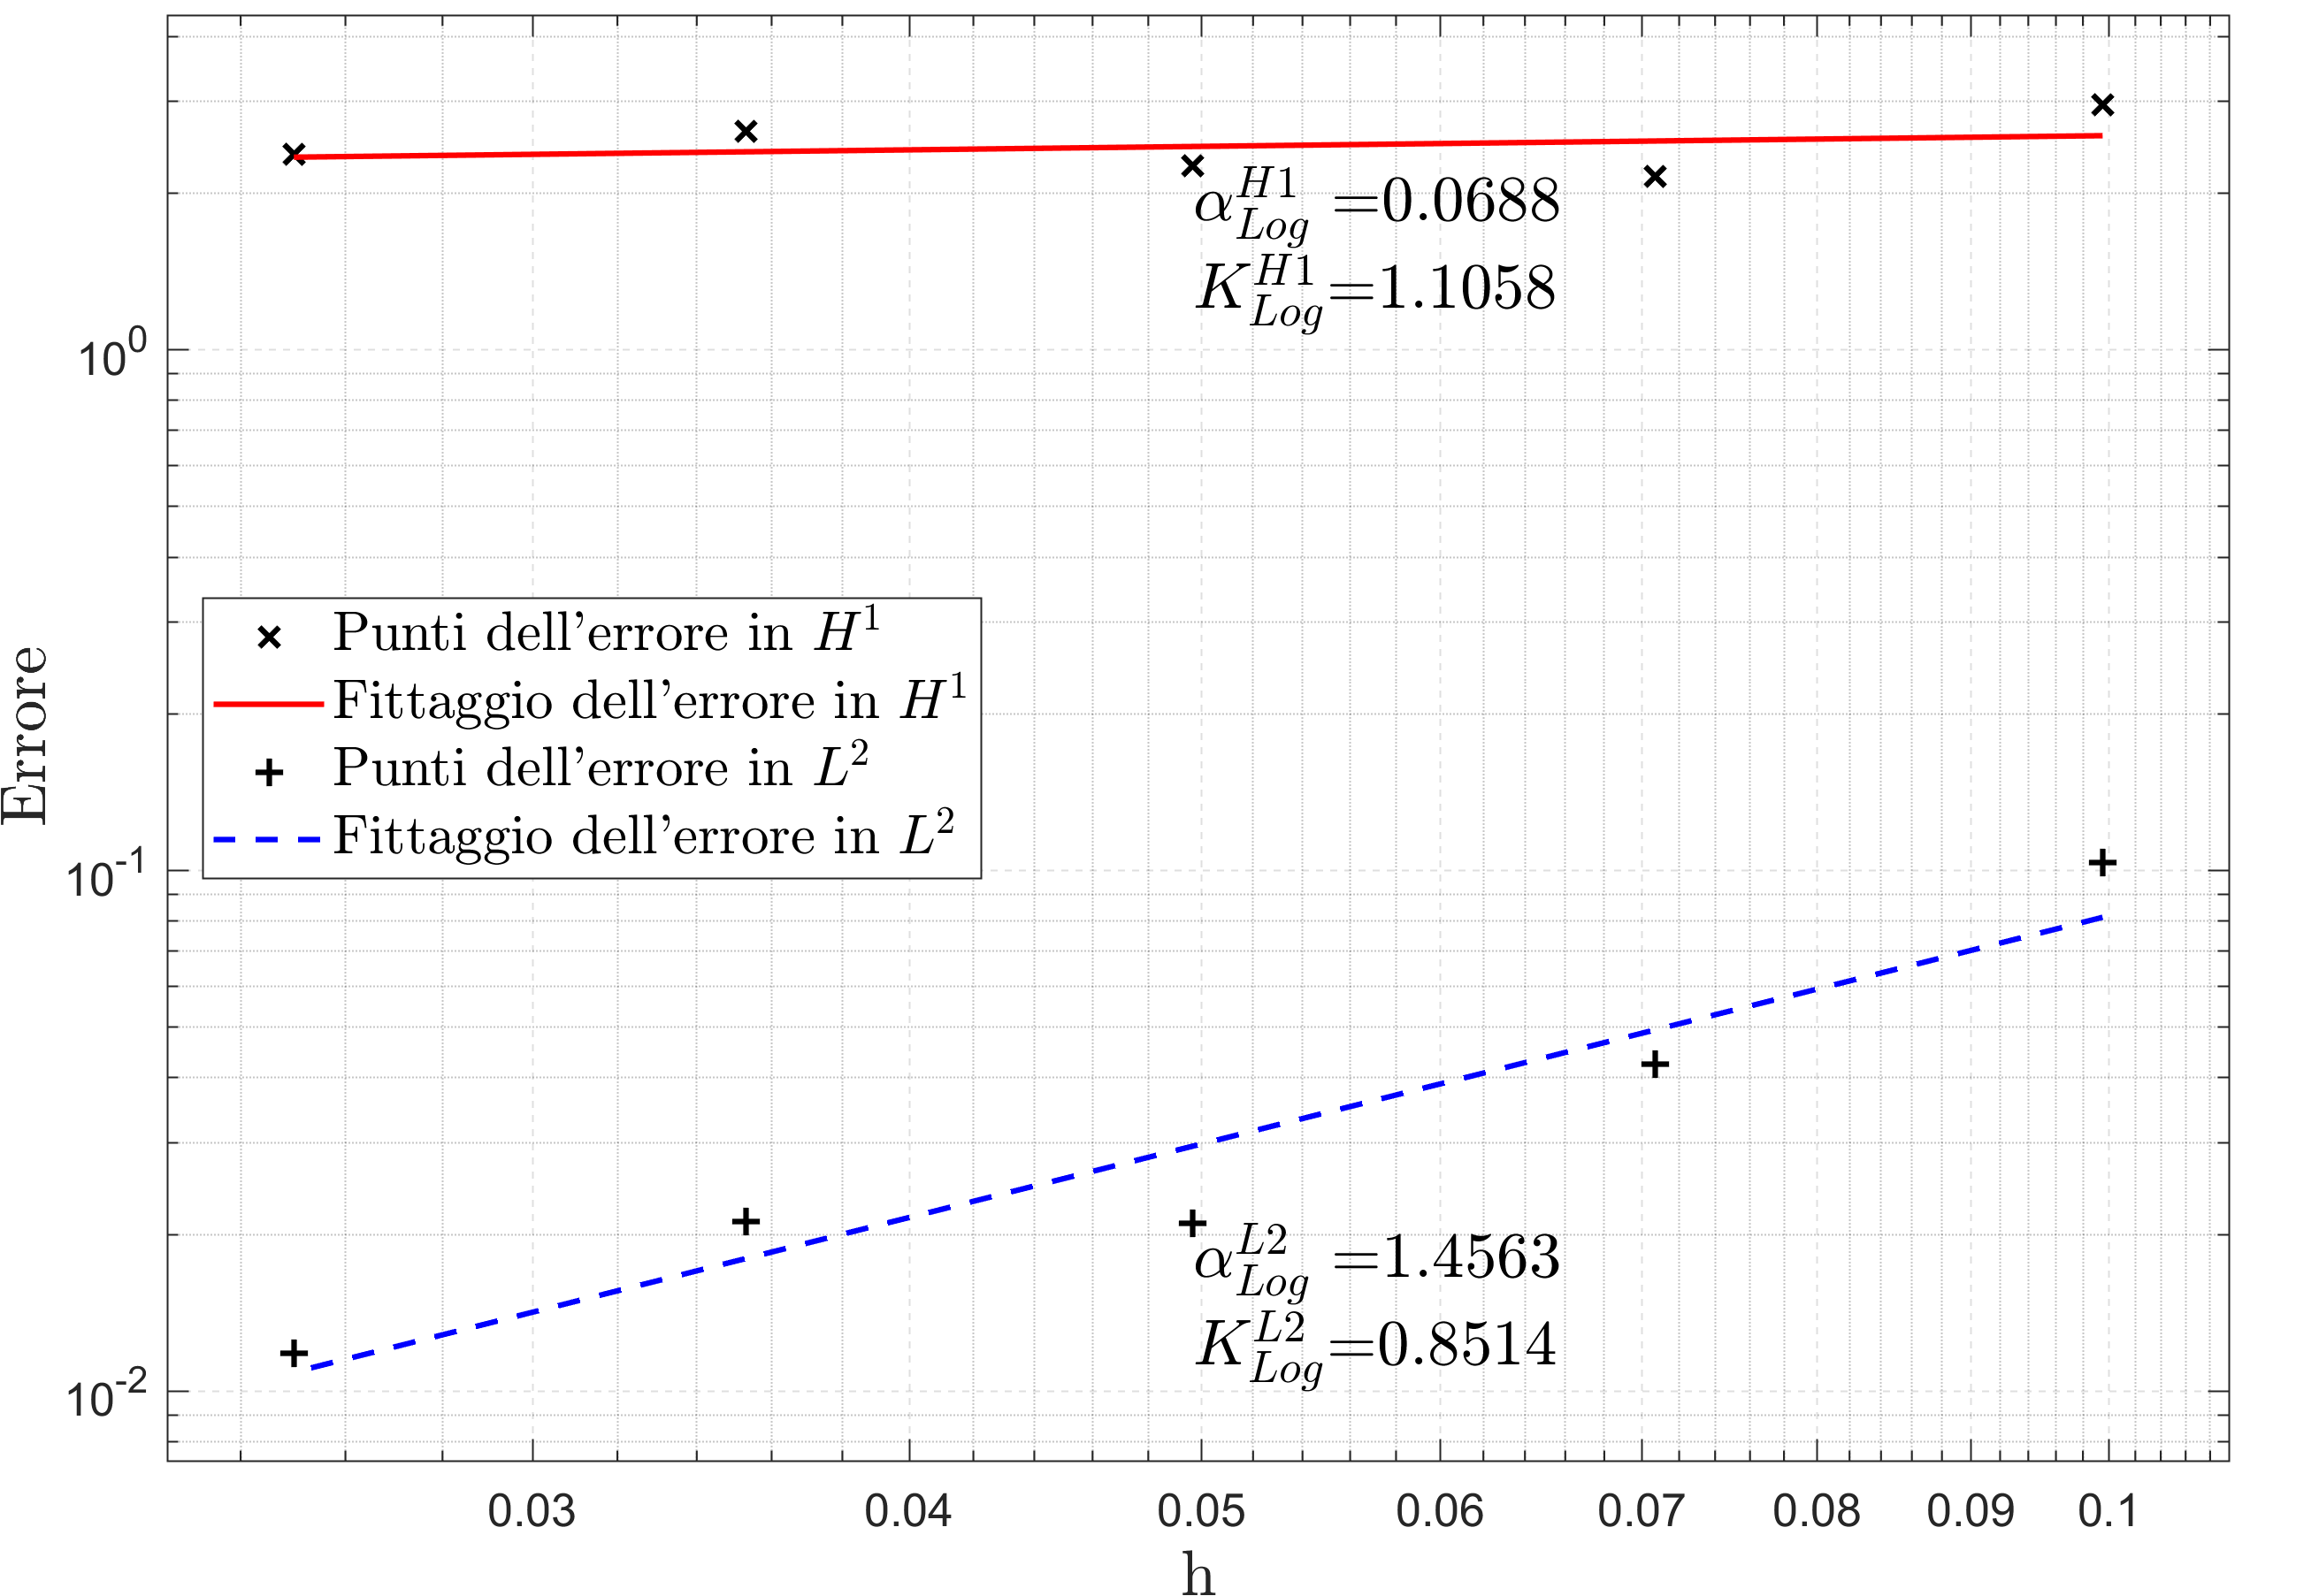
\includegraphics[width=\dimIm]{../Immagini/SDC2_P2_CS_ErrLog_AMax=0.01_NSim=5.png}
                            \caption{Errore dei $\mathbb{P}_2$ in scala logaritmica con \textit{SUPG}.}
                            \label{figSDC2ErroreP2Log}
                        \end{subfigure}
                    }
                    \caption{Nelle Figg. \ref{figSDC2TriangolazioniEsatta}-\ref{figSDC2TriangolazioniApprossimataP2} sono mostrate le soluzioni dell'SDC2: una esatta e le altre approssimate con \textit{SUPG}; invece nelle \ref{figSDC2ErroreP1Lin}-\ref{figSDC2ErroreP2Log} sono illustrati in due scale diverse gli errori in norma $H^1$ ed $L^2$ con \textit{SUPG}. I parametri dati a \textit{BBTR} sono spiegati nel $\S$\ref{parPremessaParametriBBTR}.}
                    \label{figSDC2}
                \end{figure*}
                %%%%%%%%%%%%%%%%%%
                %%%%%%%%%%%%%%%%%%
                %%%%%%%%%%%%%%%%%%

                %%%%%%%%%%%%%%%%%%%%%%%%%%%%
                %%% Tabella degli errori %%%
                %%%%%%%%%%%%%%%%%%%%%%%%%%%%
                {
                \setlength{\belowcaptionskip}{-0.3cm}
                \begin{table*}[t]
                    \centering
    
                        % Spaziatura globale
                    \newcommand{\lunST}{0.49\textwidth} % Lunghezza sottotabella
                    \newcommand{\sepTabC}{\hspace{0.5cm}}  % Separazione delle tabelle
    
                        % Spaziatura locale
                    \newcommand{\sepCol}{\hspace{5pt}}
                    \newcommand{\lungTst}{0.5cm}
                    \renewcommand{\arraystretch}{1.5}
                    
                    \makebox[\textwidth][c]{
                    \begin{subtable}[t]{\lunST}
                        \centering
                        \begin{tabular}{c@{}|@{\sepCol}c@{\sepCol}c@{\sepCol}c@{\sepCol}c@{\sepCol}c}
                            $h$&
                            \notaSci{9.95}{-2}&
                            \notaSci{7.07}{-2}&
                            \notaSci{4.97}{-2}&
                            \notaSci{3.53}{-2}&
                            \notaSci{2.50}{-2}\\
                            \hline
                            $\text{err}_{L^2}^{\mathbb P_1}$&
                                \notaSci{4.54}{-1}&
                                \notaSci{1.98}{-1}&
                                \notaSci{9.96}{-2}&
                                \notaSci{4.38}{-2}&
                                \notaSci{2.19}{-2}\\
                            $\text{err}_{H^1}^{\mathbb P_1}$&
                                \notaSci{1.57}{+1}&
                                \notaSci{1.20}{+1}&
                                \notaSci{8.23}{+0}&
                                \notaSci{5.52}{+0}&
                                \notaSci{3.87}{+0}\\
                            $\text{err}_{L^2}^{\mathbb P_2}$&
                                \notaSci{4.04}{-2}&
                                \notaSci{1.38}{-2}&
                                \notaSci{5.01}{-3}&
                                \notaSci{1.65}{-3}&
                                \notaSci{5.59}{-4}\\
                            $\text{err}_{H^1}^{\mathbb P_2}$&
                                \notaSci{2.31}{+0}&
                                \notaSci{1.25}{+0}&
                                \notaSci{6.24}{-1}&
                                \notaSci{2.99}{-1}&
                                \notaSci{1.41}{-1}
                        \end{tabular}
                        \caption{SDC1.}
                        \label{tabErroriSDC1}
                    \end{subtable}
                    \sepTabC
                    \begin{subtable}[t]{\lunST}
                        \centering
                        \begin{tabular}{c@{}|@{\sepCol}c@{\sepCol}c@{\sepCol}c@{\sepCol}c@{\sepCol}c}
                            $h$&
                            \notaSci{9.95}{-2}&
                            \notaSci{7.07}{-2}&
                            \notaSci{4.97}{-2}&
                            \notaSci{3.53}{-2}&
                            \notaSci{2.50}{-2}\\
                            \hline
                            $\text{err}_{L^2}^{\mathbb P_1}$&
                            \notaSci{1.74}{-1}&
                            \notaSci{1.01}{-1}&
                            \notaSci{7.22}{-2}&
                            \notaSci{4.11}{-2}&
                            \notaSci{2.56}{-2}\\
                            $\text{err}_{H^1}^{\mathbb P_1}$&
                            \notaSci{5.00}{+0}&
                            \notaSci{3.64}{+0}&
                            \notaSci{2.91}{+0}&
                            \notaSci{2.73}{+0}&
                            \notaSci{2.52}{+0}\\
                            $\text{err}_{L^2}^{\mathbb P_2}$&
                            \notaSci{1.04}{-1}&
                            \notaSci{4.24}{-2}&
                            \notaSci{2.11}{-2}&
                            \notaSci{2.12}{-2}&
                            \notaSci{1.18}{-2}\\
                            $\text{err}_{H^1}^{\mathbb P_2}$&
                            \notaSci{2.96}{+0}&
                            \notaSci{2.15}{+0}&
                            \notaSci{2.25}{+0}&
                            \notaSci{2.63}{+0}&
                            \notaSci{2.38}{+0}
                        \end{tabular}
                        \caption{Dati relativi all'errore nell'SDC2.}
                        \label{tabErroriSDC2}
                    \end{subtable}
                    }
                    \caption{Dati relativi all'errore nell'SDC.}
                    \label{tabErroriSDC}
                \end{table*}
                }
                %%%%%%%%%%%%%%%%%%%%%%%%%%%%
                %%%%%%%%%%%%%%%%%%%%%%%%%%%%
                %%%%%%%%%%%%%%%%%%%%%%%%%%%%
                

                Pertanto nel metodo \textit{SUPG} le funzioni tèste differiscono [almeno nella parte omogenea del \teqref{eqPSVariazionaleDiscreto}{[PV]$_\text{h}$}] da quelle di forma, ossia dalle funzioni di base \textit{globali} $\varphi_j$ che ricostruiscono la funzione a partire dalla soluzione $\mathbf u$ ricavata dalla \eqref{eqSistemaAlgebrico}.
                
                Seguendo gli stessi passaggi nel $\S$\ref{parAnalisiErrore}, dal \teqref{eqPSVariazionaleDiscreto}{[PV]$^{\text{s}}_\text{h}$} si ricava il sistema algebrico
                %
                \begin{equation*}
                    \mathbf A_\text{s}\mathbf u\equiv
                    (\mathbf A+\mathbf S)\mathbf u=
                    \mathbf f+\mathbf f_\text{s}+\mathbf g-\mathbf A_D\mathbf u_D
                    \equiv\mathbf b_\text{s},
                    \label{eqSistemaAlgebricoStabilizzato}
                \end{equation*}
                %
                che stabilizza sia la matrice di rigidezza che il termine noto
                
                Si nota inoltre che è possibile dare una forma alla matrice $\mathbf S$ e al vettore $\mathbf f_\text{s}$     rispetto alle funzioni di base \textit{globali} $\varphi_j$, come fatto per le altre matrici nella \eqref{eqSistemaAlgebricoDefinizioneMatrici} perché la viscosità artificiale $\tau_T$ nella \eqref{eqViscositaArtificiale} è definita per ogni EF; in effetti il modo di costruire non solo queste matrici stabilizzanti, ma in realtà tutte quelle mostrate nella \eqref{eqSistemaAlgebricoDefinizioneMatrici}, sebbene le formule suggeriscano altrimenti, è quello di scandire gli EF e tramite le forme \textit{locali} delle funzioni di base $\boldsymbol\Phi_{\hat\jmath}^T=\varphi_j\vert_T$ (ove $\hat\jmath$ è l'indice locale mentre $j$ è il suo corrispettivo globale) calcolare il relativo contributo alle matrici (si v. \cite{dispenseMEDèPA} $\S5.3$ per maggiori dettagli).

                Per quanto riguarda l'SDC1 Nella Fig. \ref{figSDC1TriangolazioniEsatta} è mostrata la soluzione esatta mentre nelle Figg. \ref{figSDC1TriangolazioniApprossimataP1} e \ref{figSDC1TriangolazioniApprossimataP2} le due approssimate mediante i $\mathbb P_1$ e i $\mathbb P_2$ rispettivamente. D'altro canto nelle Figg. \ref{figSDC1ErroreP1Lin} e \ref{figSDC1ErroreP1Log} è illustrato l'andamento dell'errore per i $\mathbb P_1$ e similmente nelle Figg. \ref{figSDC1ErroreP2Lin} e \ref{figSDC1ErroreP2Log} per i $\mathbb P_2$ (i relativi dati si trovano nella Tab. \ref{tabErroriSDC1})

                Tutti questi andamenti corrispondono a quanto detto nel $\S$\ref{parAnalisiErrore}, eppure si può notare súbito qualcosa di strano: l'errore in $H^1$ è elevato, rimanendo sopra l'unità coi $\mathbb P_1$ mentre coi $\mathbb P_2$ ne scende al di sotto solo dalla terza iterazione in poi; e siccome il corrispettivo errore in $L^2$ è invece molto basso, ciò suggerisce che si riesce a cogliere bene la funzione punto per punto, ma non i suoi gradienti; in altre parole vi sono oscillazioni, possibilmente in corrispondenza del bordo destro ove la funzione decade ripidamente.

                Invece per quanto riguarda l'SDC2 Nella Fig. \ref{figSDC1TriangolazioniEsatta} è mostrata la soluzione esatta mentre nelle Figg. \ref{figSDC1TriangolazioniApprossimataP1} e \ref{figSDC1TriangolazioniApprossimataP2} le due approssimate mediante i $\mathbb P_1$ e i $\mathbb P_2$. D'altro canto nelle Figg. \ref{figSDC1ErroreP1Lin} e \ref{figSDC1ErroreP1Log} è illustrato l'andamento dell'errore per i $\mathbb P_1$ e similmente nelle Figg. \ref{figSDC1ErroreP2Lin} e \ref{figSDC1ErroreP2Log} per i $\mathbb P_2$ (i relativi dati si trovano nella Tab. \ref{tabErroriSDC2}).
                
                Contrariamente all'SDC1, questi andamenti non corrispondono affatto a quanto detto nel $\S$\ref{parAnalisiErrore}; anzi, si ripresenta pure la differenza significativa tra la norma in $H^1$ e quella in $L^2$, e quindi delle oscillazioni; in effetti esse sono visibili nella Fig. \ref{figSDC1TriangolazioniApprossimataP2} e perdurano anche nella soluzione approssimata migliore, mostrata nella Fig. \ref{figSDC2SoluzioneMiglioreP2}, in cui è chiaro che siano trasversali alla direzione di $\boldsymbol\beta$.

                \begin{figure}[H]
                    \centering 
                    \newcommand{\dimIm}{\linewidth}
                    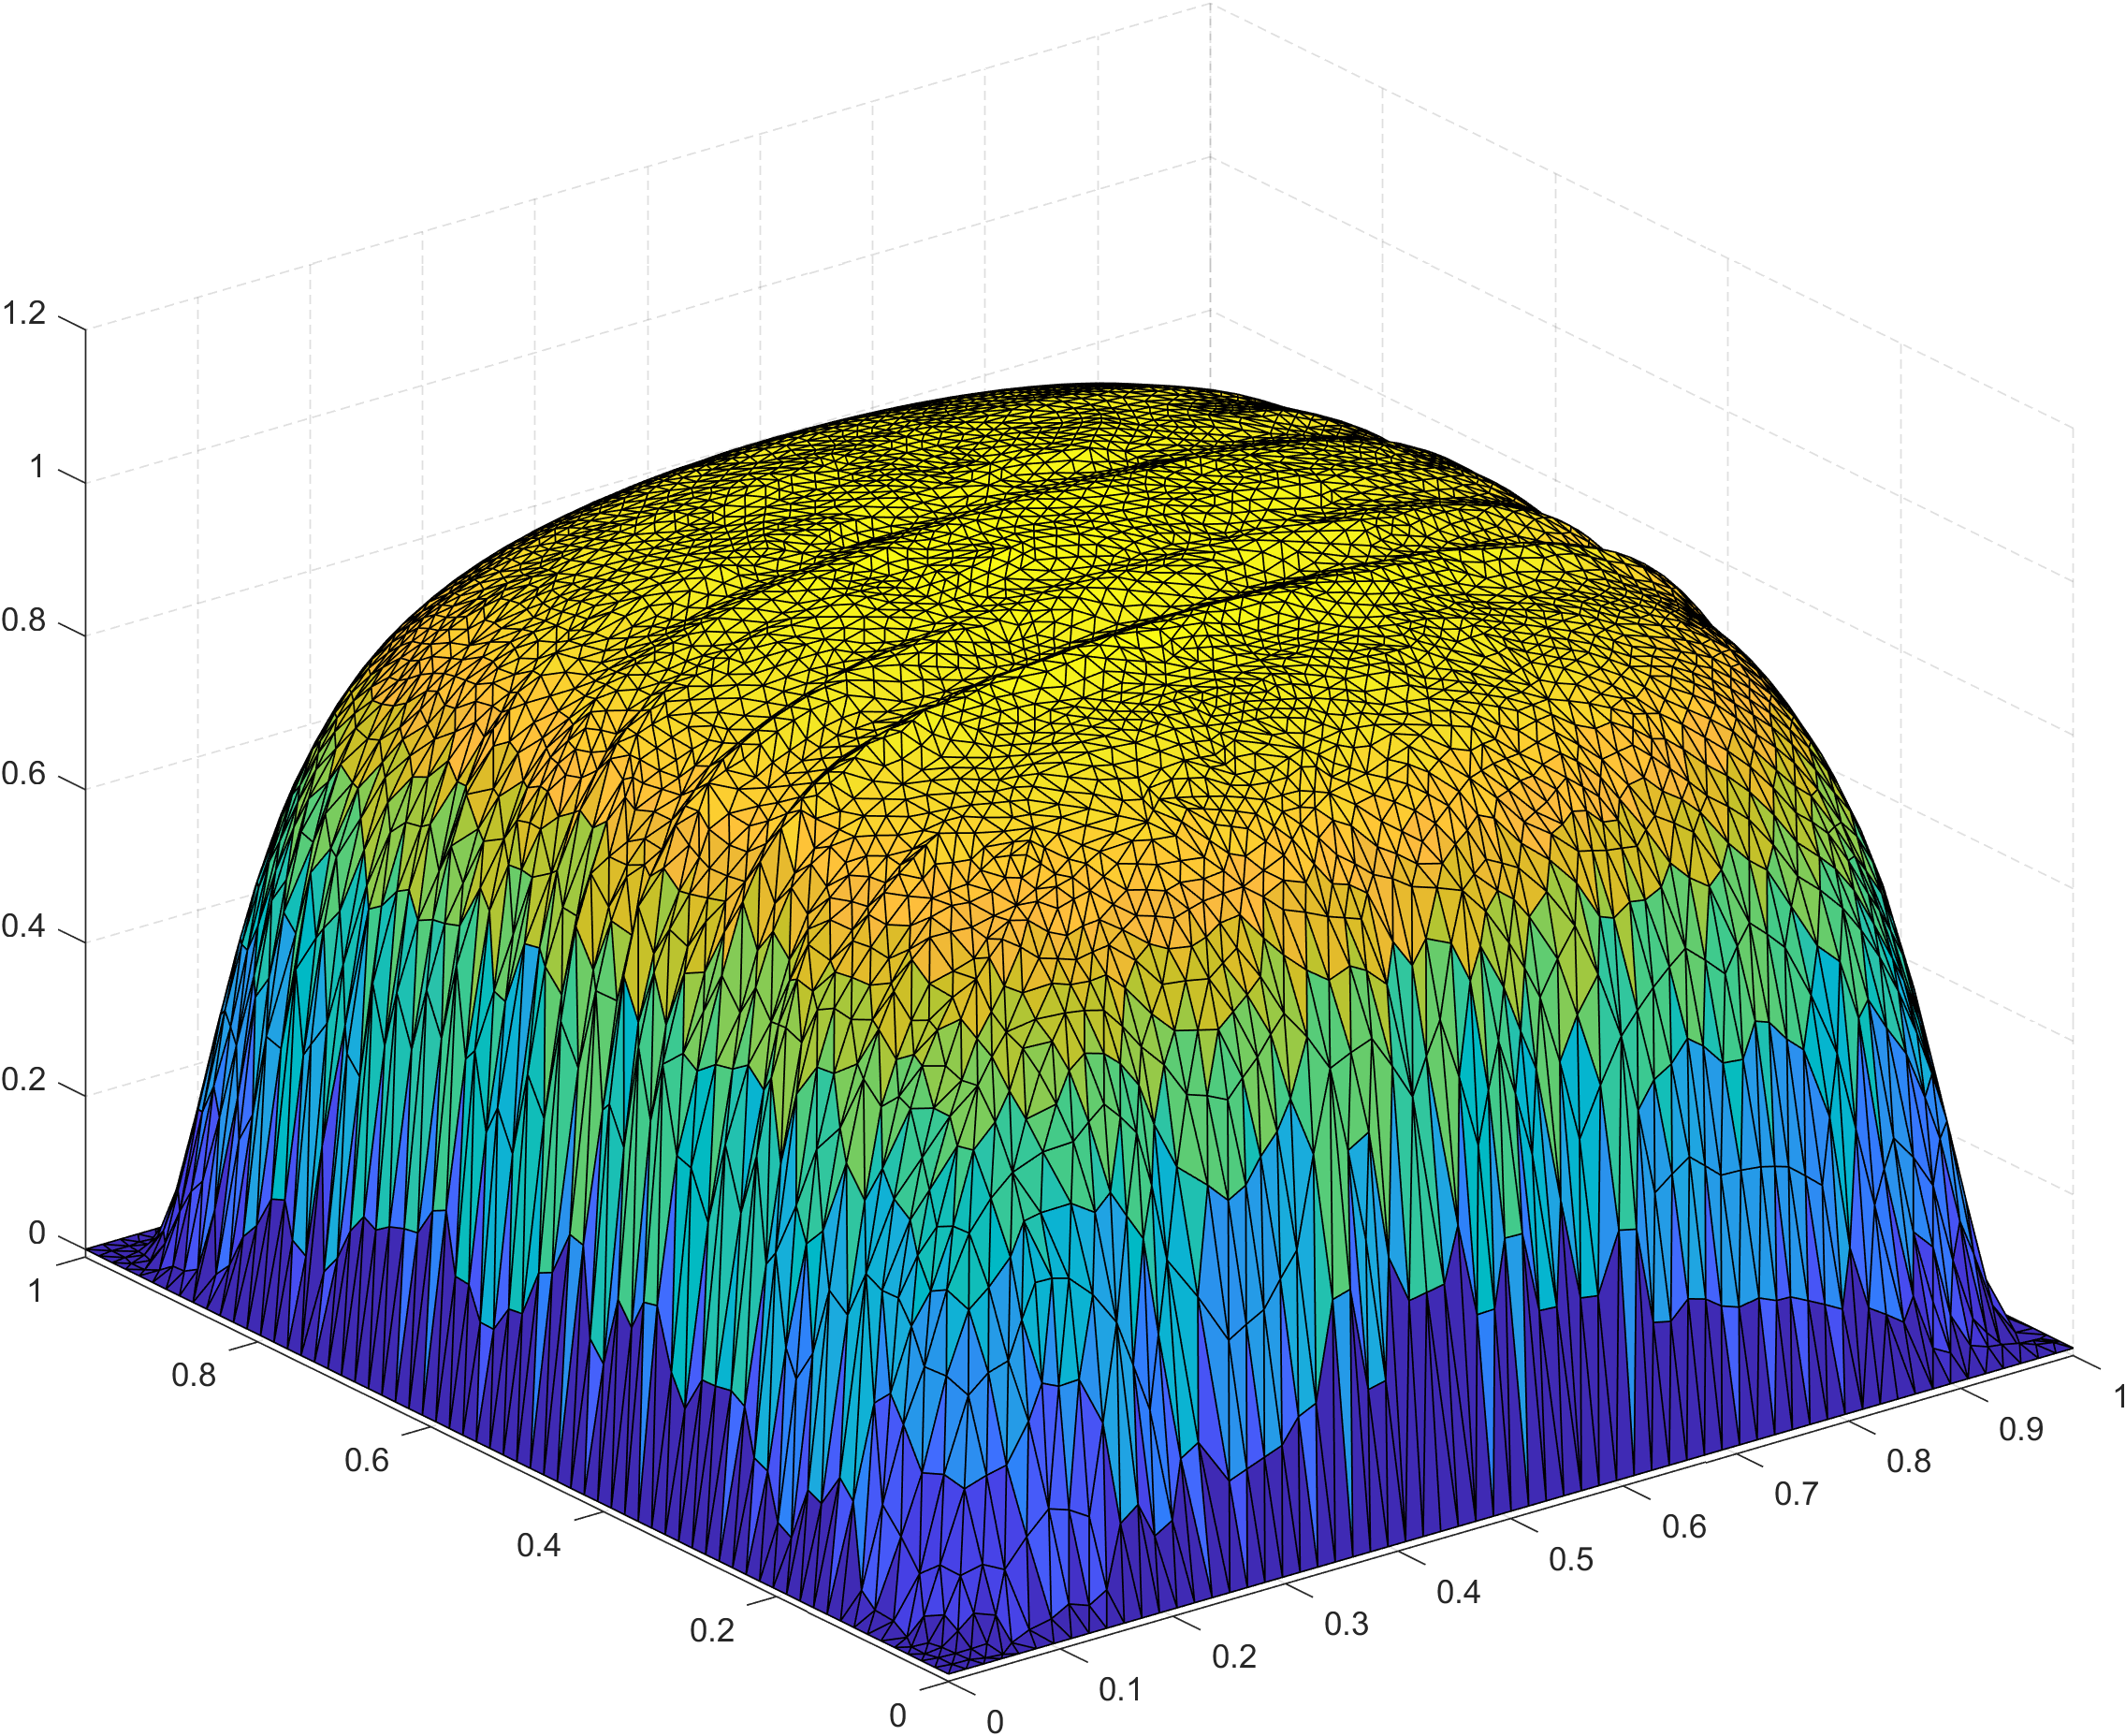
\includegraphics[width=\dimIm]{../Immagini/SDC2_CS_P2_Migliore.png}
                    \caption{Soluzione migliore dell'SDC2 coi $\mathbb P_2$ ed $h_5=0.025$.}
                    \label{figSDC2SoluzioneMiglioreP2}
                \end{figure}
                
                Tutto ciò mette in luce che la stabilizzazione \textit{SUPG}, seppure possa evitare il peggio come nelle Figg. \ref{figSDC1Instabile} e \ref{figSDC2Instabile}, non è perfetta e può faticare con funzioni particolarmente cattive come la \eqref{eqSoluzioneEsattaSDC2}.
                
                Si nota infine che nel caso in cui $\boldsymbol\beta$ sia entrante in un lato di Neumann, si perde la coercività della forma bilineare descritta dalla \eqref{eqOperatoreBilinearePSVariazionale} (si v. \cite{dispenseMEDèPA} Esempio 1.2.2 a p. 17 per maggiori dettagli) a causa della contraddizione
                %
                \begin{equation*}
                    \boldsymbol \beta\cdot\mathbf n\ge0\text{ in }\Gamma_N,
                \end{equation*}
                %
                poiché nel lato considerato vale {$\SpaziaturaMate{1}{2}{3}\boldsymbol\beta\cdot\mathbf n<0$}, con $\mathbf n$ versore normale uscente dal dominio $\Omega$. E infatti in tal caso, ossia unitamente all'alto valore del numero di Péclet, si ha instabilità proprio lungo il lato di Neumann e quindi la divergenza della soluzione approssimata, come si può vedere nelle Figg. \ref{figSDC1BetaEntrante} e \ref{figSDC2BetaEntrante}.

                {\setlength{\intextsep}{0pt}
                \begin{figure}[H]
                    \centering 
                    \newcommand{\lungSF}{.5\linewidth}
                    \newcommand{\dimIm}{\linewidth}
                    \makebox[\linewidth][c]{
                        \begin{subfigure}[t]{\lungSF}
                            \centering
                            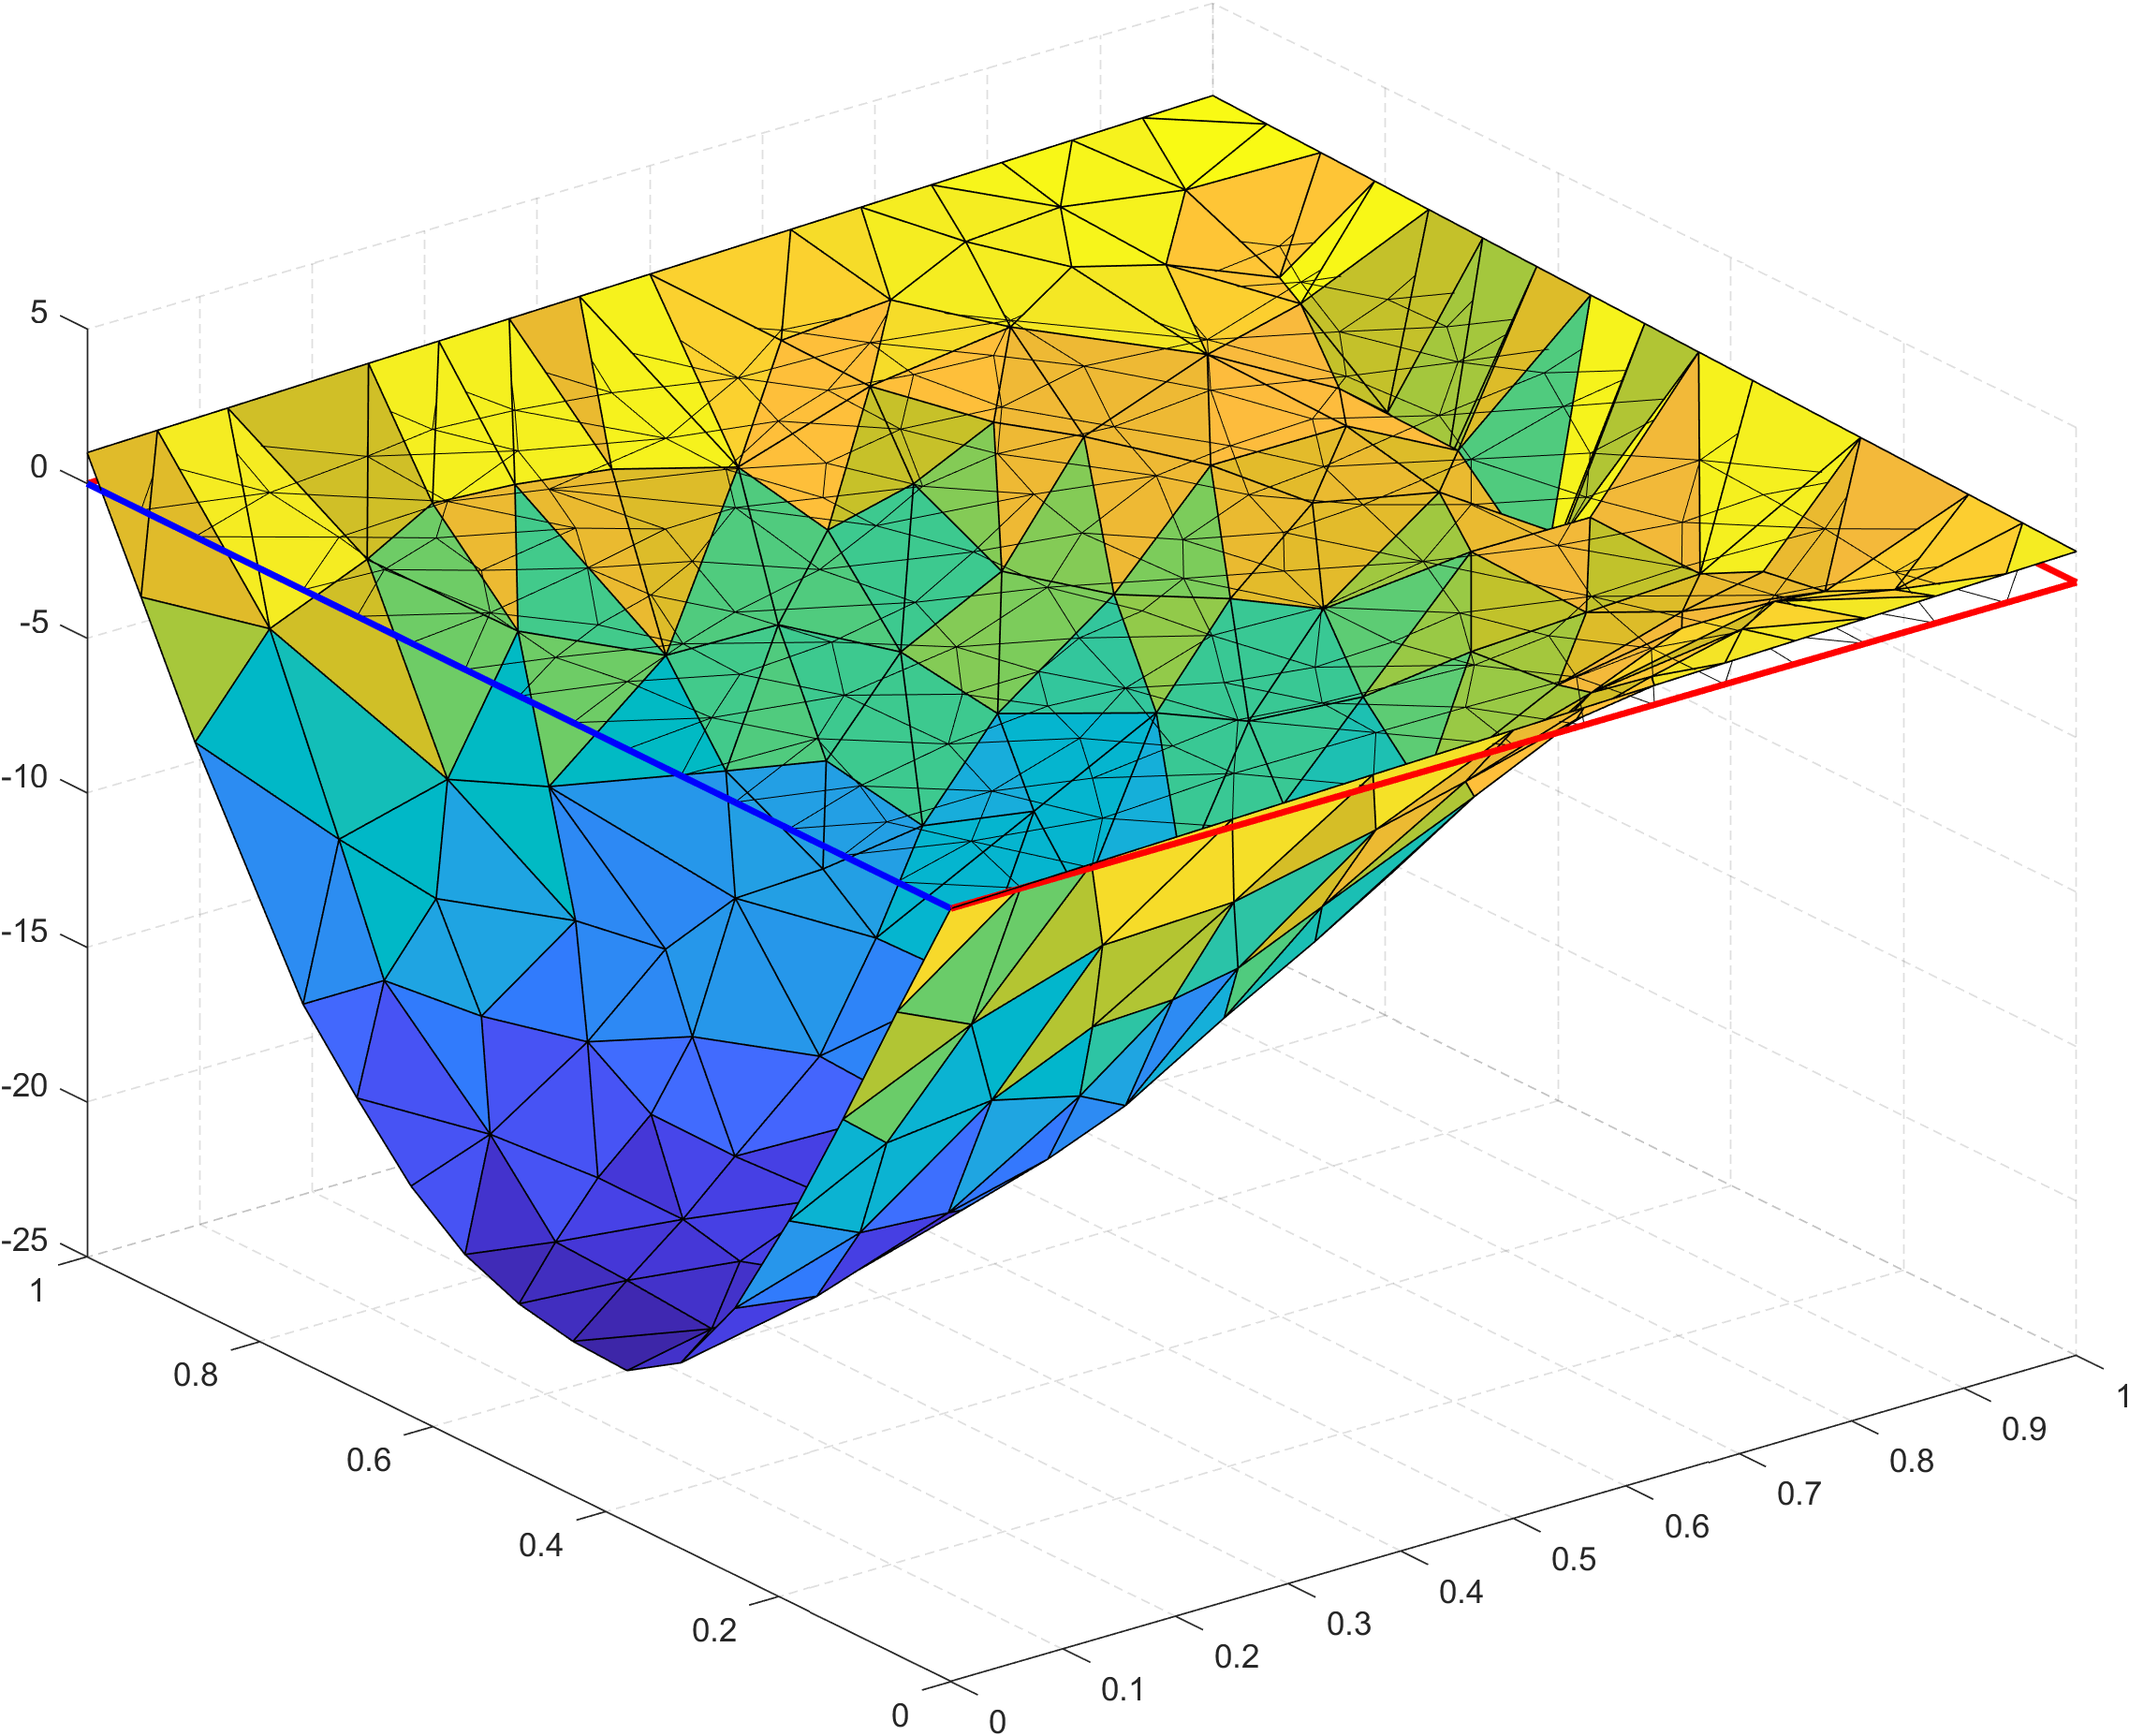
\includegraphics[width=\dimIm]{../Immagini/SDC1_CS_P1_AMax=0.005_Beta_Entrante.png}
                            \caption{Coi $\mathbb{P}_1$.}
                            \label{figSDC1BetaEntranteP1}
                        \end{subfigure}
                        \begin{subfigure}[t]{\lungSF}
                            \centering
                            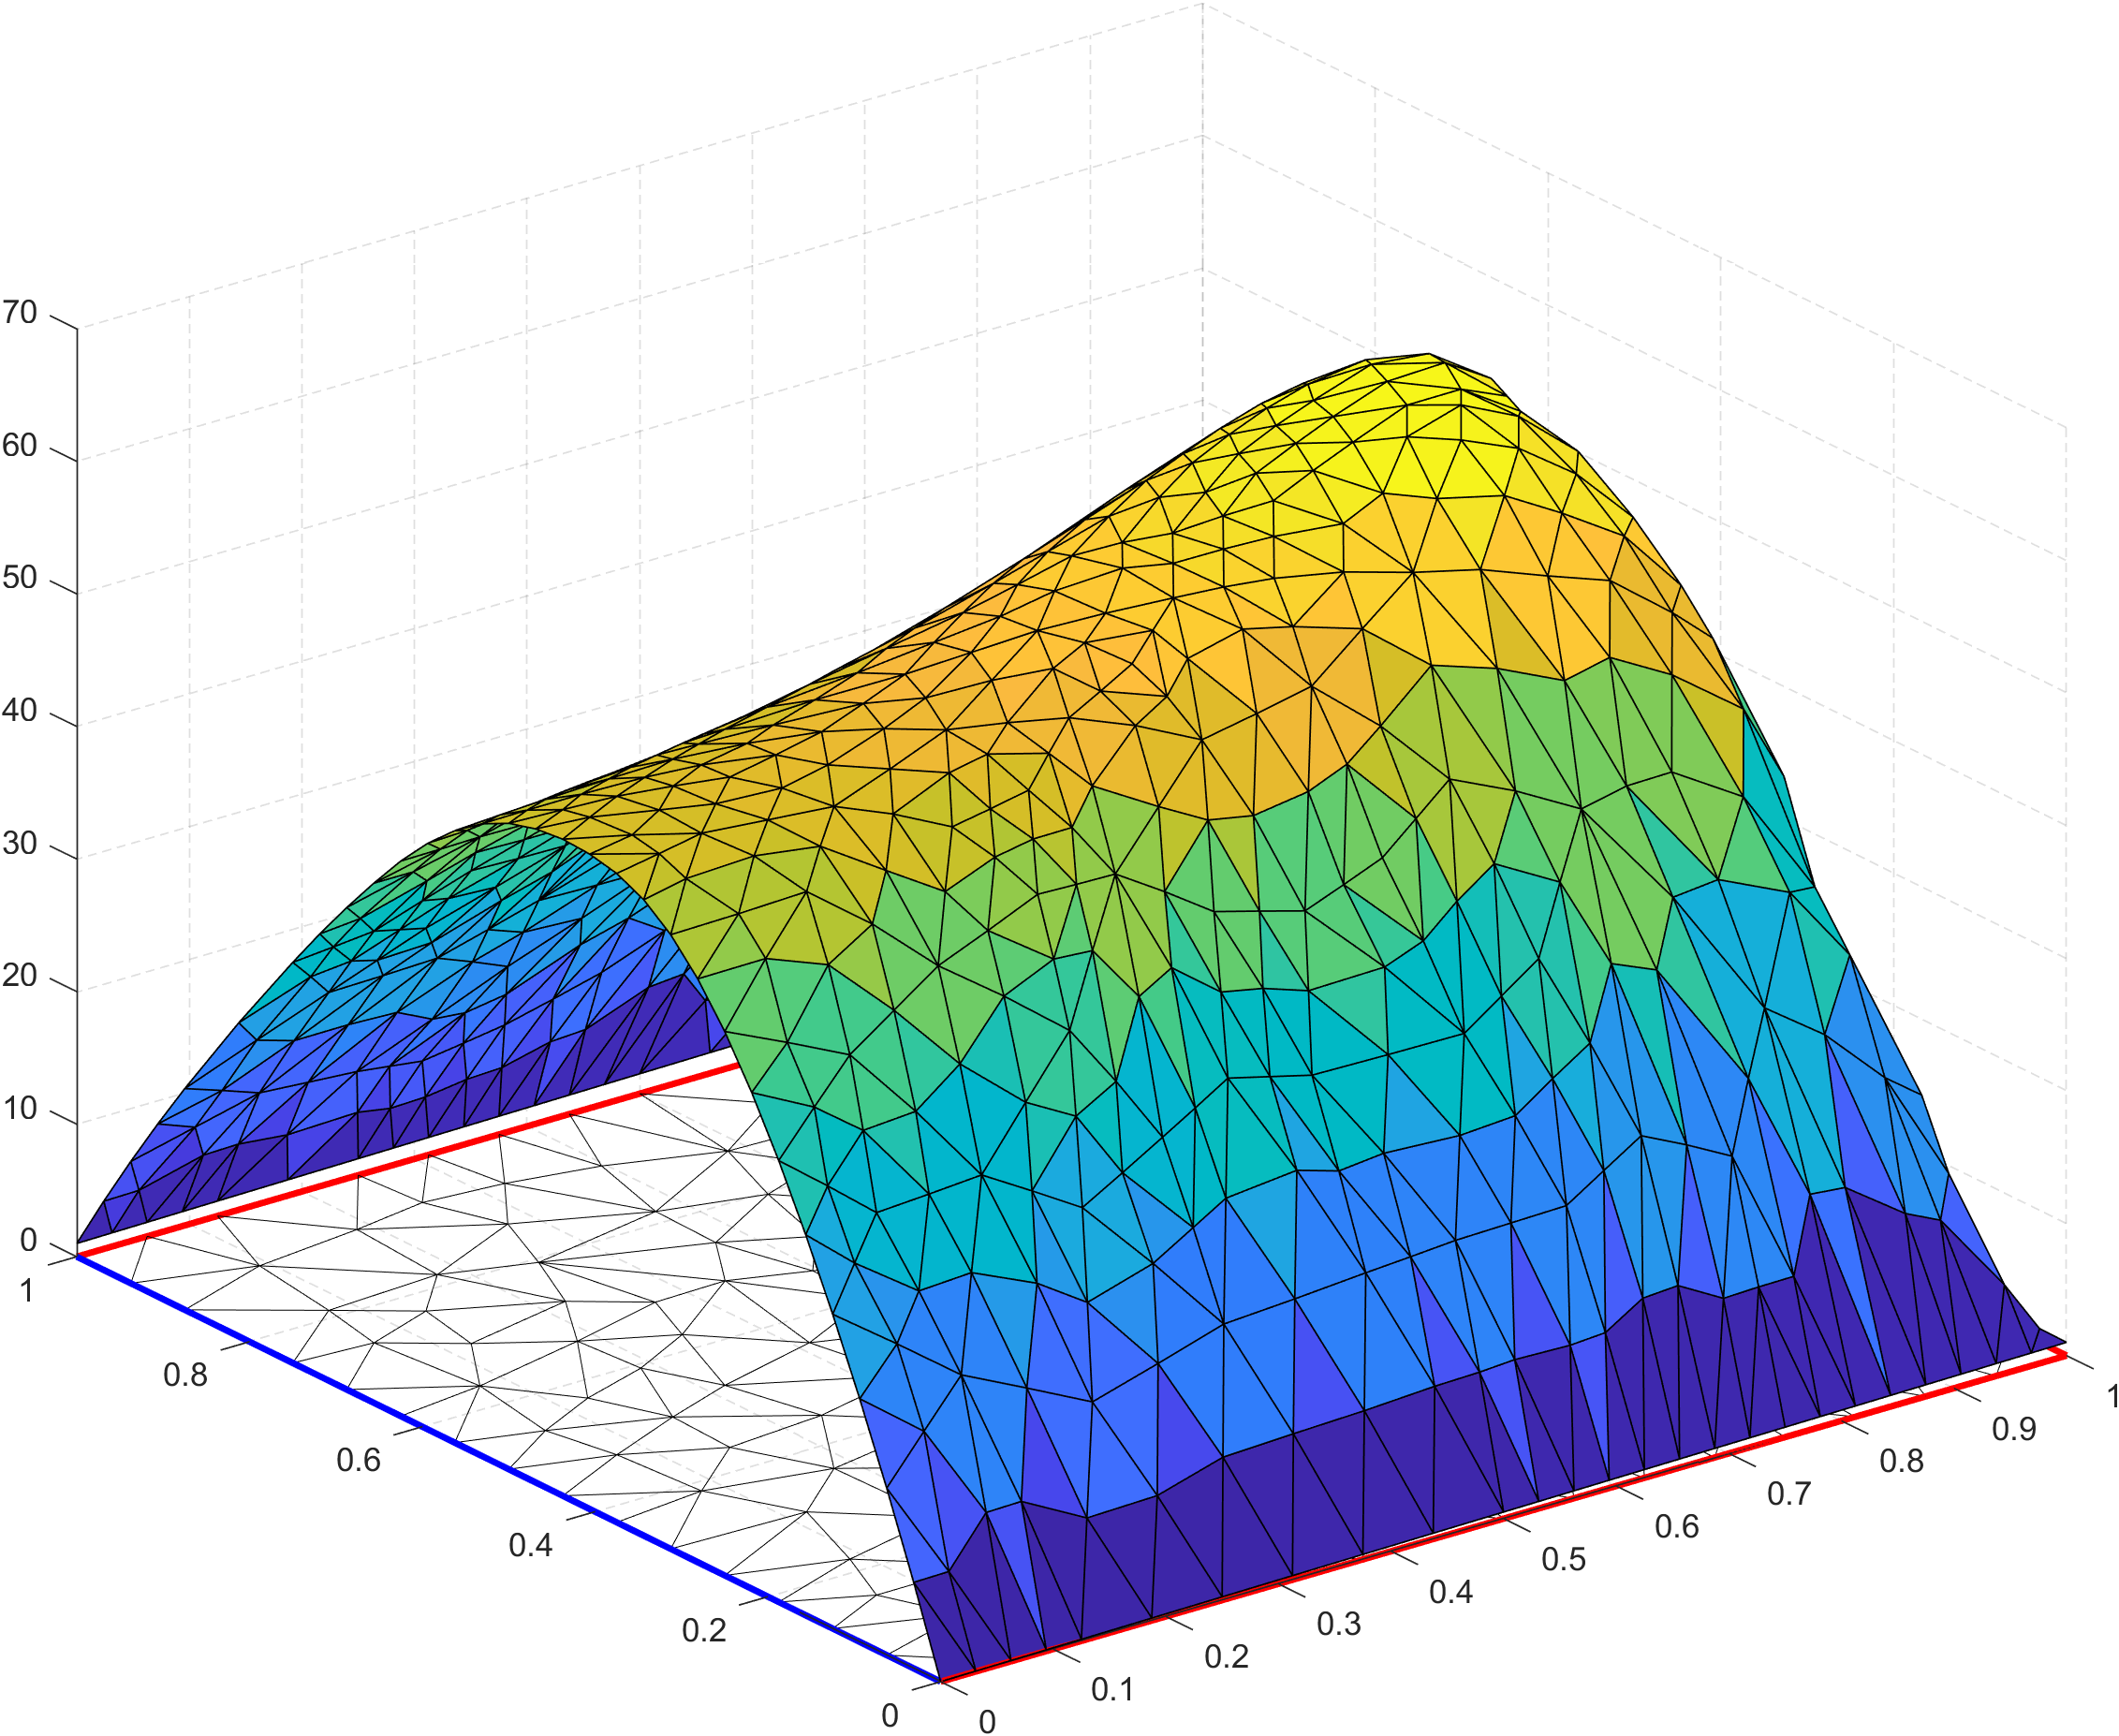
\includegraphics[width=\dimIm]{../Immagini/SDC1_CS_P2_AMax=0.005_Beta_Entrante.png}
                            \caption{Coi $\mathbb{P}_2$.}
                            \label{figSDC1BetaEntranteP2}
                        \end{subfigure}
                    }
                    \caption{Soluzioni qualitative dell'SDC1 con $\boldsymbol\beta$ entrante.}
                    \label{figSDC1BetaEntrante}
                \end{figure}
                \begin{figure}[H]
                    \centering 
                    \newcommand{\lungSF}{.5\linewidth}
                    \newcommand{\dimIm}{\linewidth}
                    \makebox[\linewidth][c]{
                        \begin{subfigure}[t]{\lungSF}
                            \centering
                            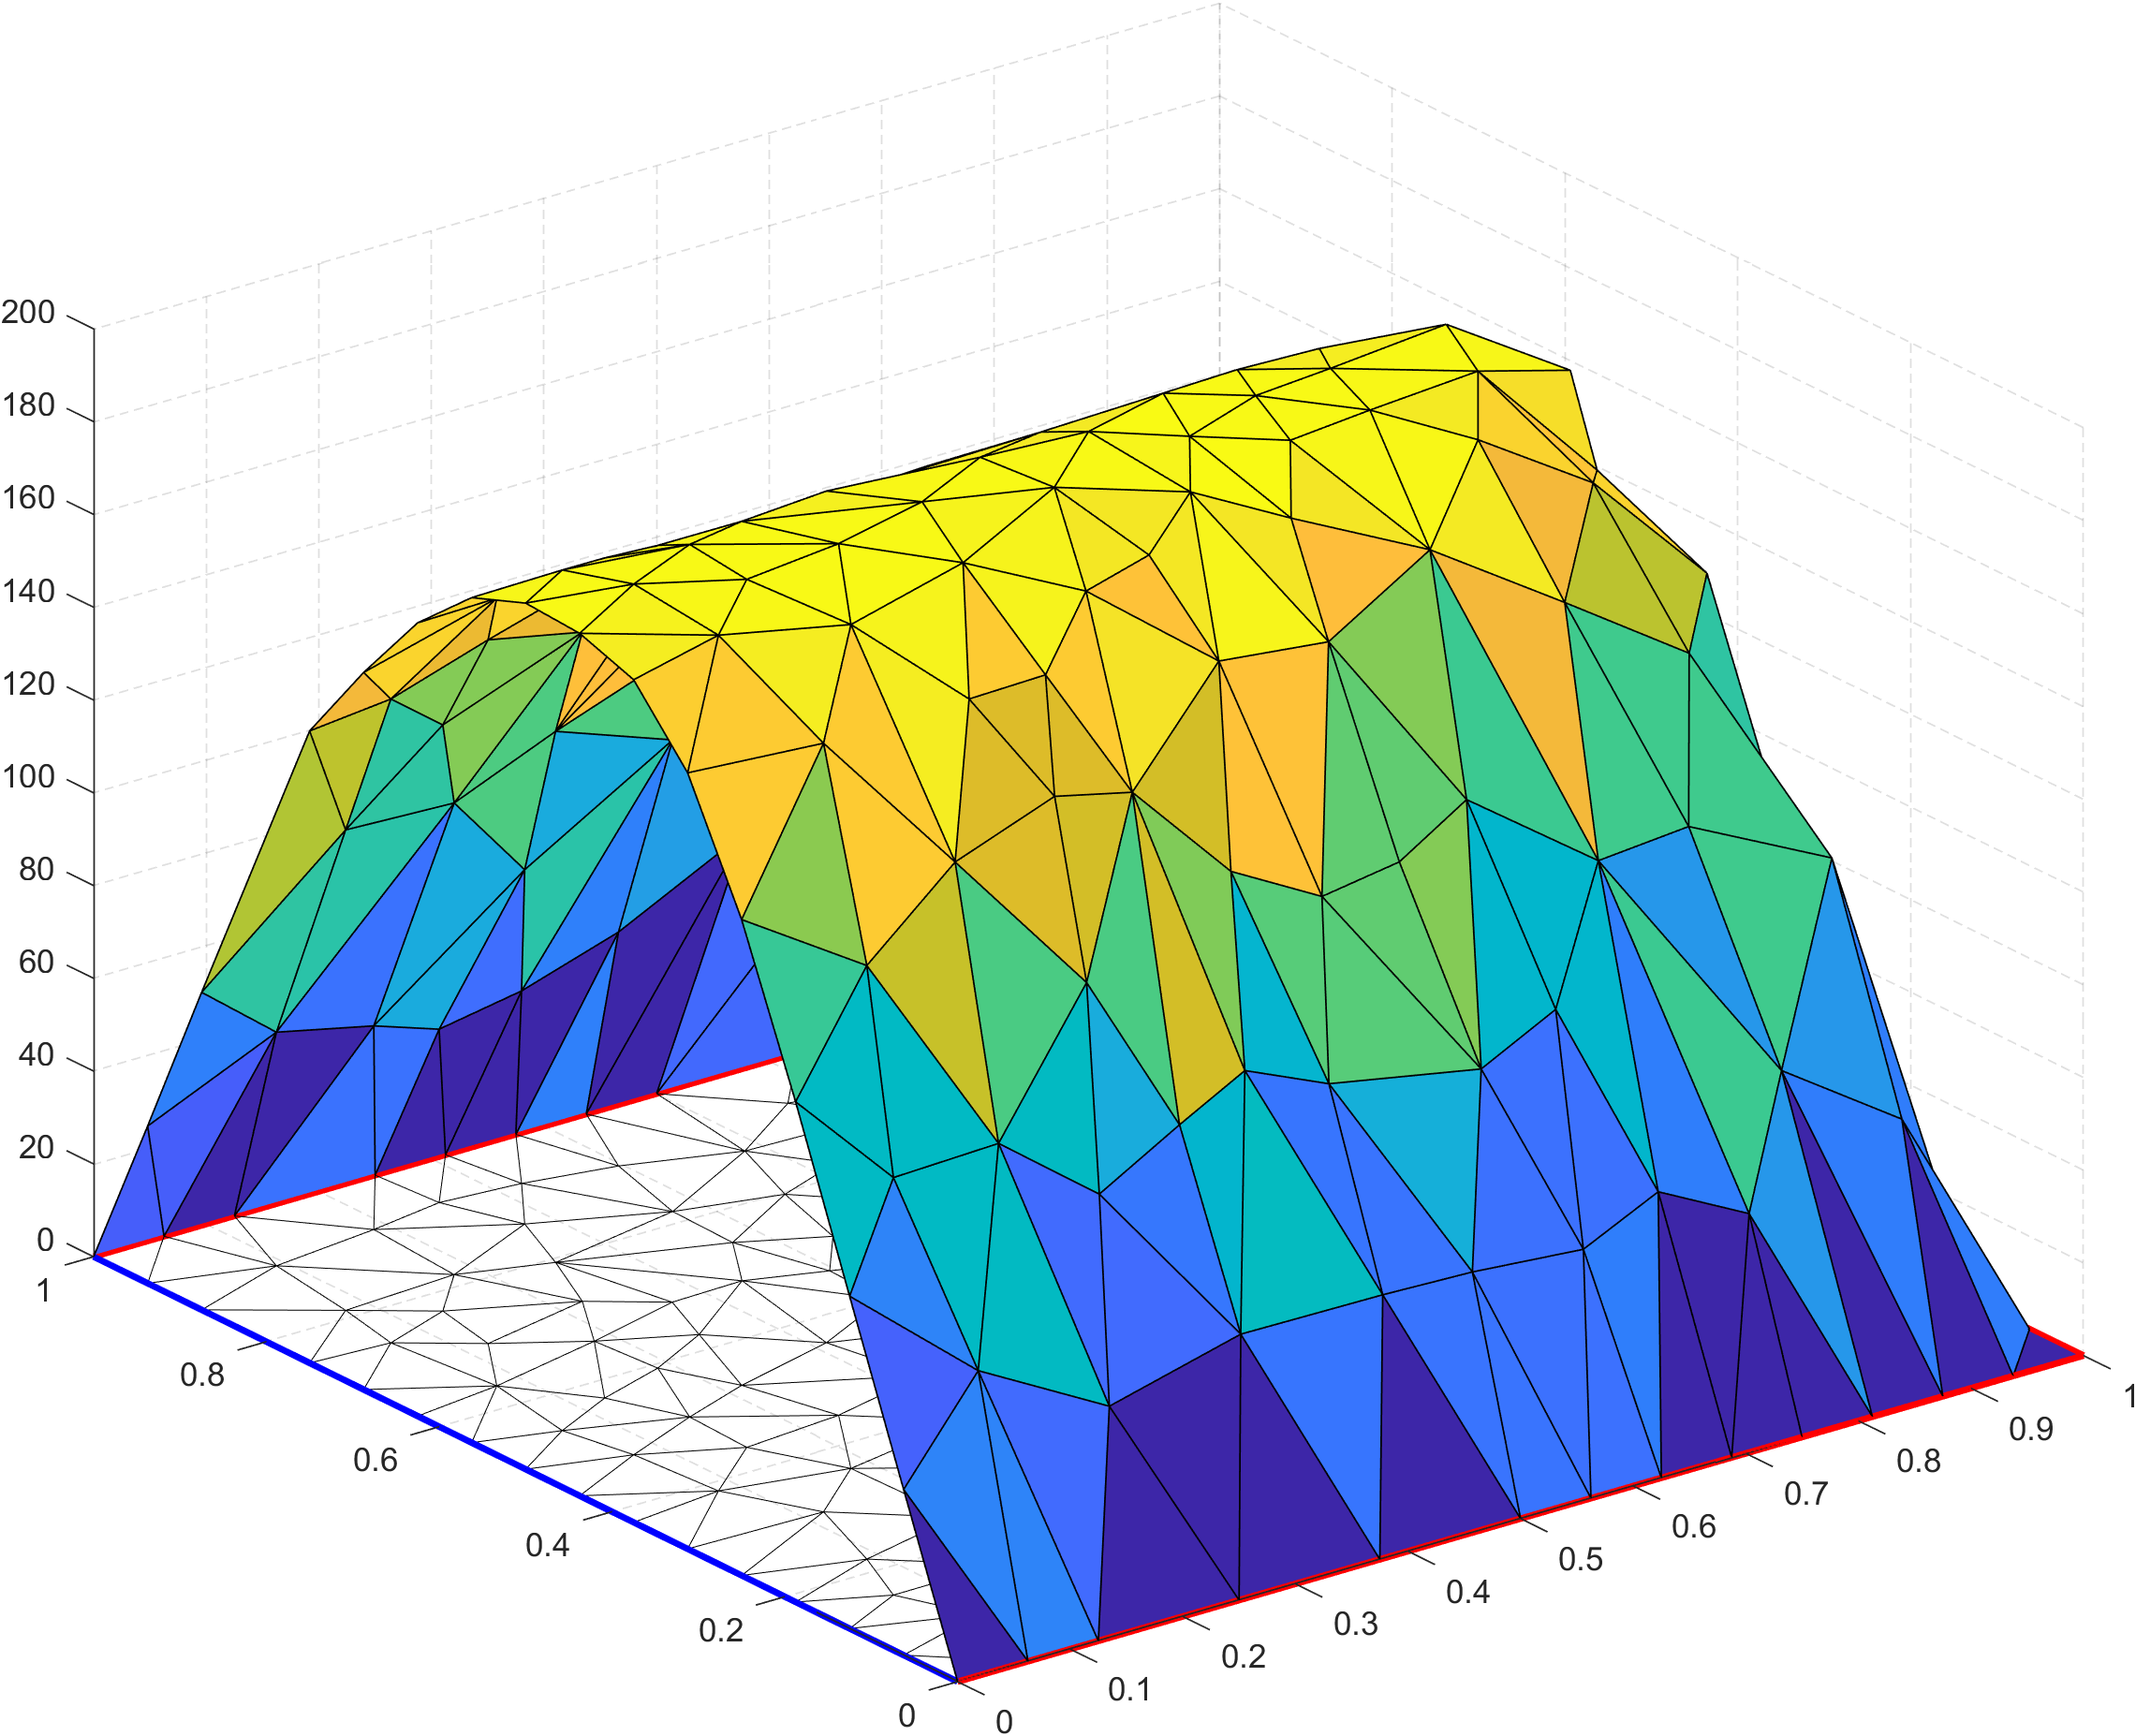
\includegraphics[width=\dimIm]{../Immagini/SDC2_CS_P1_AMax=0.005_Beta_Entrante.png}
                            \caption{Coi $\mathbb{P}_1$.}
                            \label{figSDC2BetaEntranteP1}
                        \end{subfigure}
                        \begin{subfigure}[t]{\lungSF}
                            \centering
                            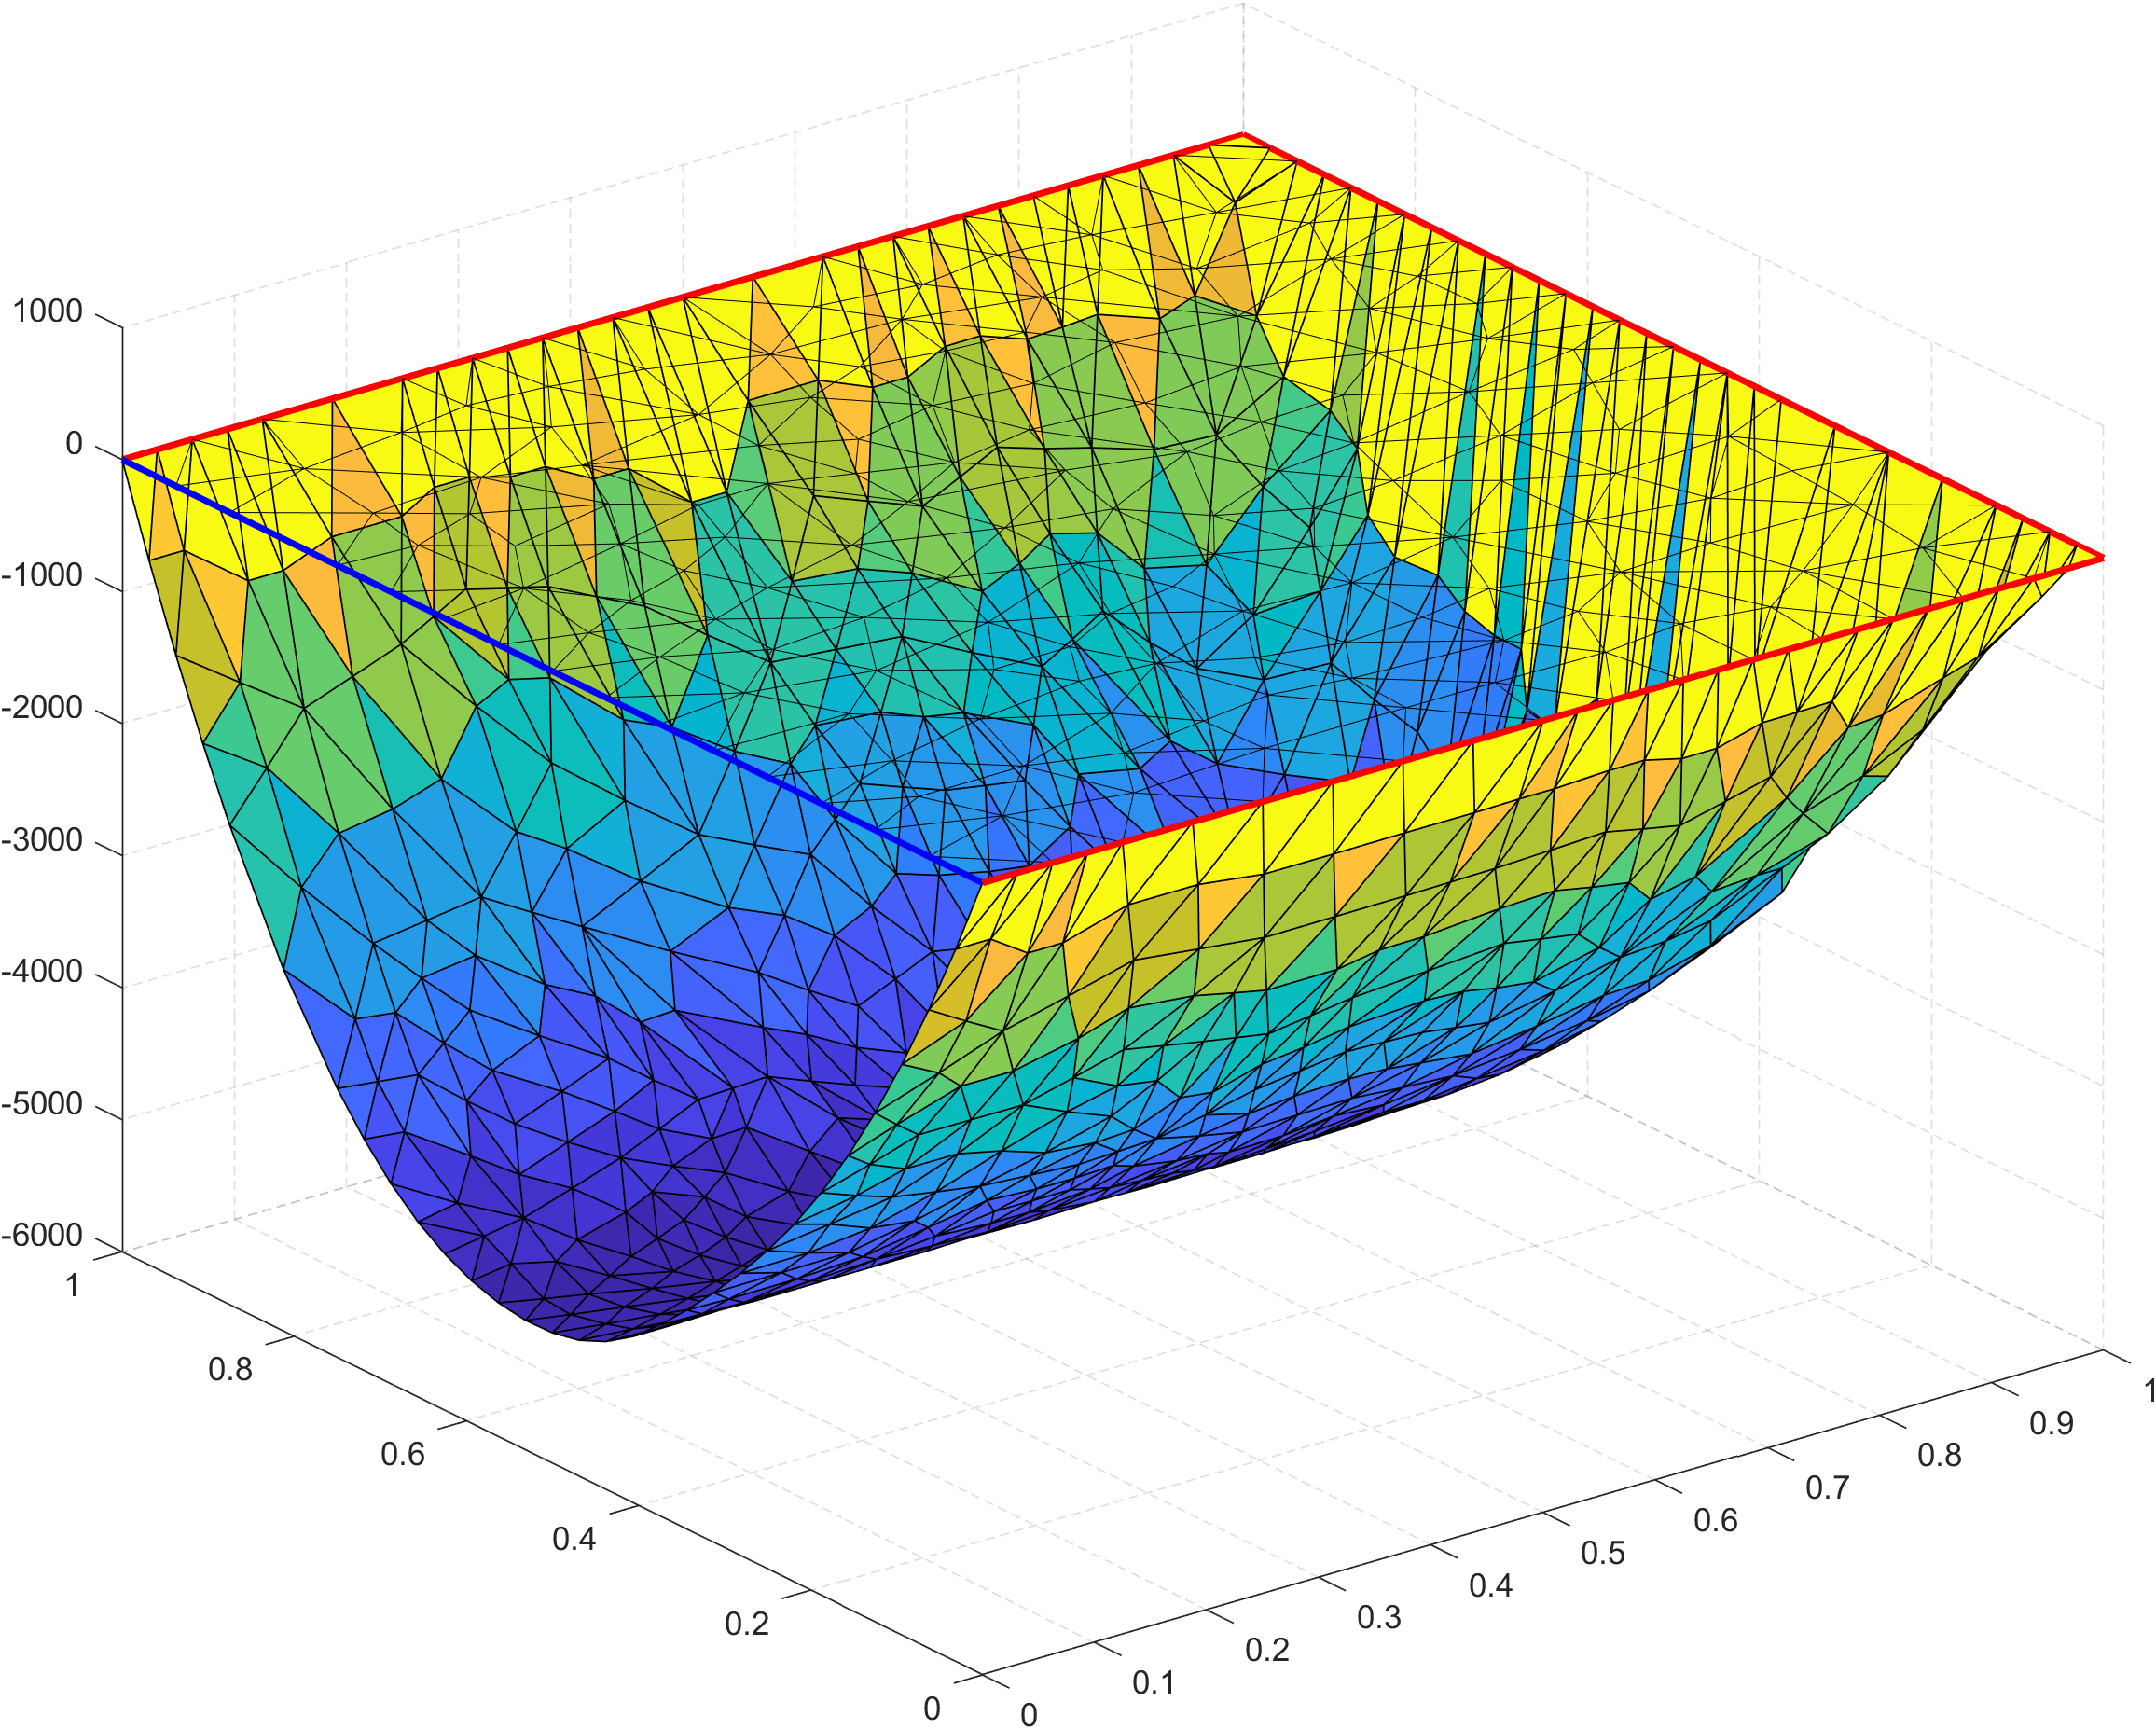
\includegraphics[width=\dimIm]{../Immagini/SDC2_CS_P2_AMax=0.005_Beta_Entrante.png}
                            \caption{Coi $\mathbb{P}_2$.}
                            \label{figSDC2BetaEntranteP2}
                        \end{subfigure}
                    }
                    \caption{Soluzioni qualitative dell'SDC2 con $\boldsymbol\beta$ entrante.}
                    \label{figSDC2BetaEntrante}
                \end{figure}
                }

    
        \subsection{Stabilità diffusione-reazione (SDR)}

            \subsubsection{Impostazione e instabilità}

                Esso consiste in un problema di diffusione debole e di reazione unitaria, ovvero
                %
                \begin{equation*}
                    \setlength{\abovedisplayskip}{5pt plus 2pt minus 2pt}  % Riduce lo spazio sopra l'equazione
                    \setlength{\belowdisplayskip}{5pt plus 2pt minus 2pt}  % Riduce lo spazio sotto l'equazione
                    \SpaziaturaMate{1}{2}{3}
                    \nu=10^{-6},\;\;\beta=(0,0)^{\top}\text{ e }\sigma=1;
                \end{equation*}
                %
                ciò equivale a trasformare il \teqref{eqProblemaStazionario}{[PS]} in
                %
                \begin{equation}
                    \left\{
                    \begin{aligned}
                        -10^{-6}\Delta u+\sigma u&=f&\text{in }&\Omega, \\
                        u&=u\vert_{\partial\Omega}&\text{su }&\partial\Omega,
                    \end{aligned}
                    \right.
                    \label{eqSDR}
                \end{equation}
                %
                ove, grazie alle funzioni
                %
                \begin{equation*}
                    \begin{gathered}
                        u_1(x,y)=e^{a(x-1)}e^{a(y-0.5)}+e^{a(x-1)}e^{-a(y-0.5)},\\
                        u_2(x,y)=e^{-ax}e^{-a(y-0.5)}+e^{-ax}e^{a(y-0.5)},\\
                    \end{gathered}
                \end{equation*}
                %
                s'impone che la prima soluzione esatta $u$ si pari a
                %
                \begin{equation}
                    u(x,y)=-u_1(x,y)u_2(x,y)-u_1(y,x)u_2(y,x)+1,
                    \label{eqSoluzioneEsattaSDR1}
                \end{equation}
                %
                con {$\SpaziaturaMate{1}{2}{3}a=10$}, e che la seconda soluzione esatta sia uguale alla \eqref{eqSoluzioneEsattaSDC2} cogli stessi parametri. Similmente a prima, queste due soluzioni saranno indicate cogli acronimi SDR1 ed SDR2 rispettivamente.

                Entrambe le funzioni sono state scelte il piú ripide possibile in tutti i bordi cosí da potenzialmente indurre instabilità; infatti si può definire un numero analogo a quello di Péclet nella \eqref{eqNumeroPeclet}
                %
                \begin{equation*}
                    Se_E=\frac{\sigma h_E^2}{6\nu}
                \end{equation*}
                %
                che coi parametri definiti risulta {$\SpaziaturaMate{1}{2}{3}Se_E\gg1$}, ovvero si è in un problema a reazione dominante che può indurre instabilità simili a quelle viste nel $\S$\ref{parInstabilitàSDC}.

                Tuttavia, come si può vedere nelle soluzioni qualitative nelle Figg. \ref{figSDR1TriangolazioniP1SA} e \ref{figSDR2TriangolazioniP1SA}, queste sembrano essere molto lievi non rovinando totalmente la soluzione come accadeva nel caso di diffusione-convezione.

                In effetti analizzando gli errori, mostrati nelle Figg. \ref{figSDR1ErroreP1LinSA} e \ref{figSDR1ErroreP1LogSA} per l'SDR1 e nelle Figg. \ref{figSDR2ErroreP1LinSA} e \ref{figSDR2ErroreP1LogSA} per l'SDR2 (i relativi dati si trovano rispettivamente nelle Tabb. \ref{tabErroriSDR1} e \ref{tabErroriSDR2}, e sono contrassegnati dalle righe coll'acronimo SA nell'ultima colonna), gli andamenti non corrispondono di certo a quanto detto nel $\S$\ref{parAnalisiErrore} però non si discostano eccessivamente dai valori teorici.
                
                
            \subsubsection{Ammassamento}

                %%%%%%%%%%%%%%%%%%
                %%% Infopagine %%%
                %%%%%%%%%%%%%%%%%%
                \begin{figure*}[p]
                    \newcommand{\distR}{\vspace{15pt}} % Distanza tra le righe
                    
                    \newcommand{\lungSF}{0.33\textwidth}
                    \newcommand{\dimIm}{4cm}
                    \makebox[\linewidth][c]{
                        \begin{subfigure}[t]{\lungSF}
                            \centering
                            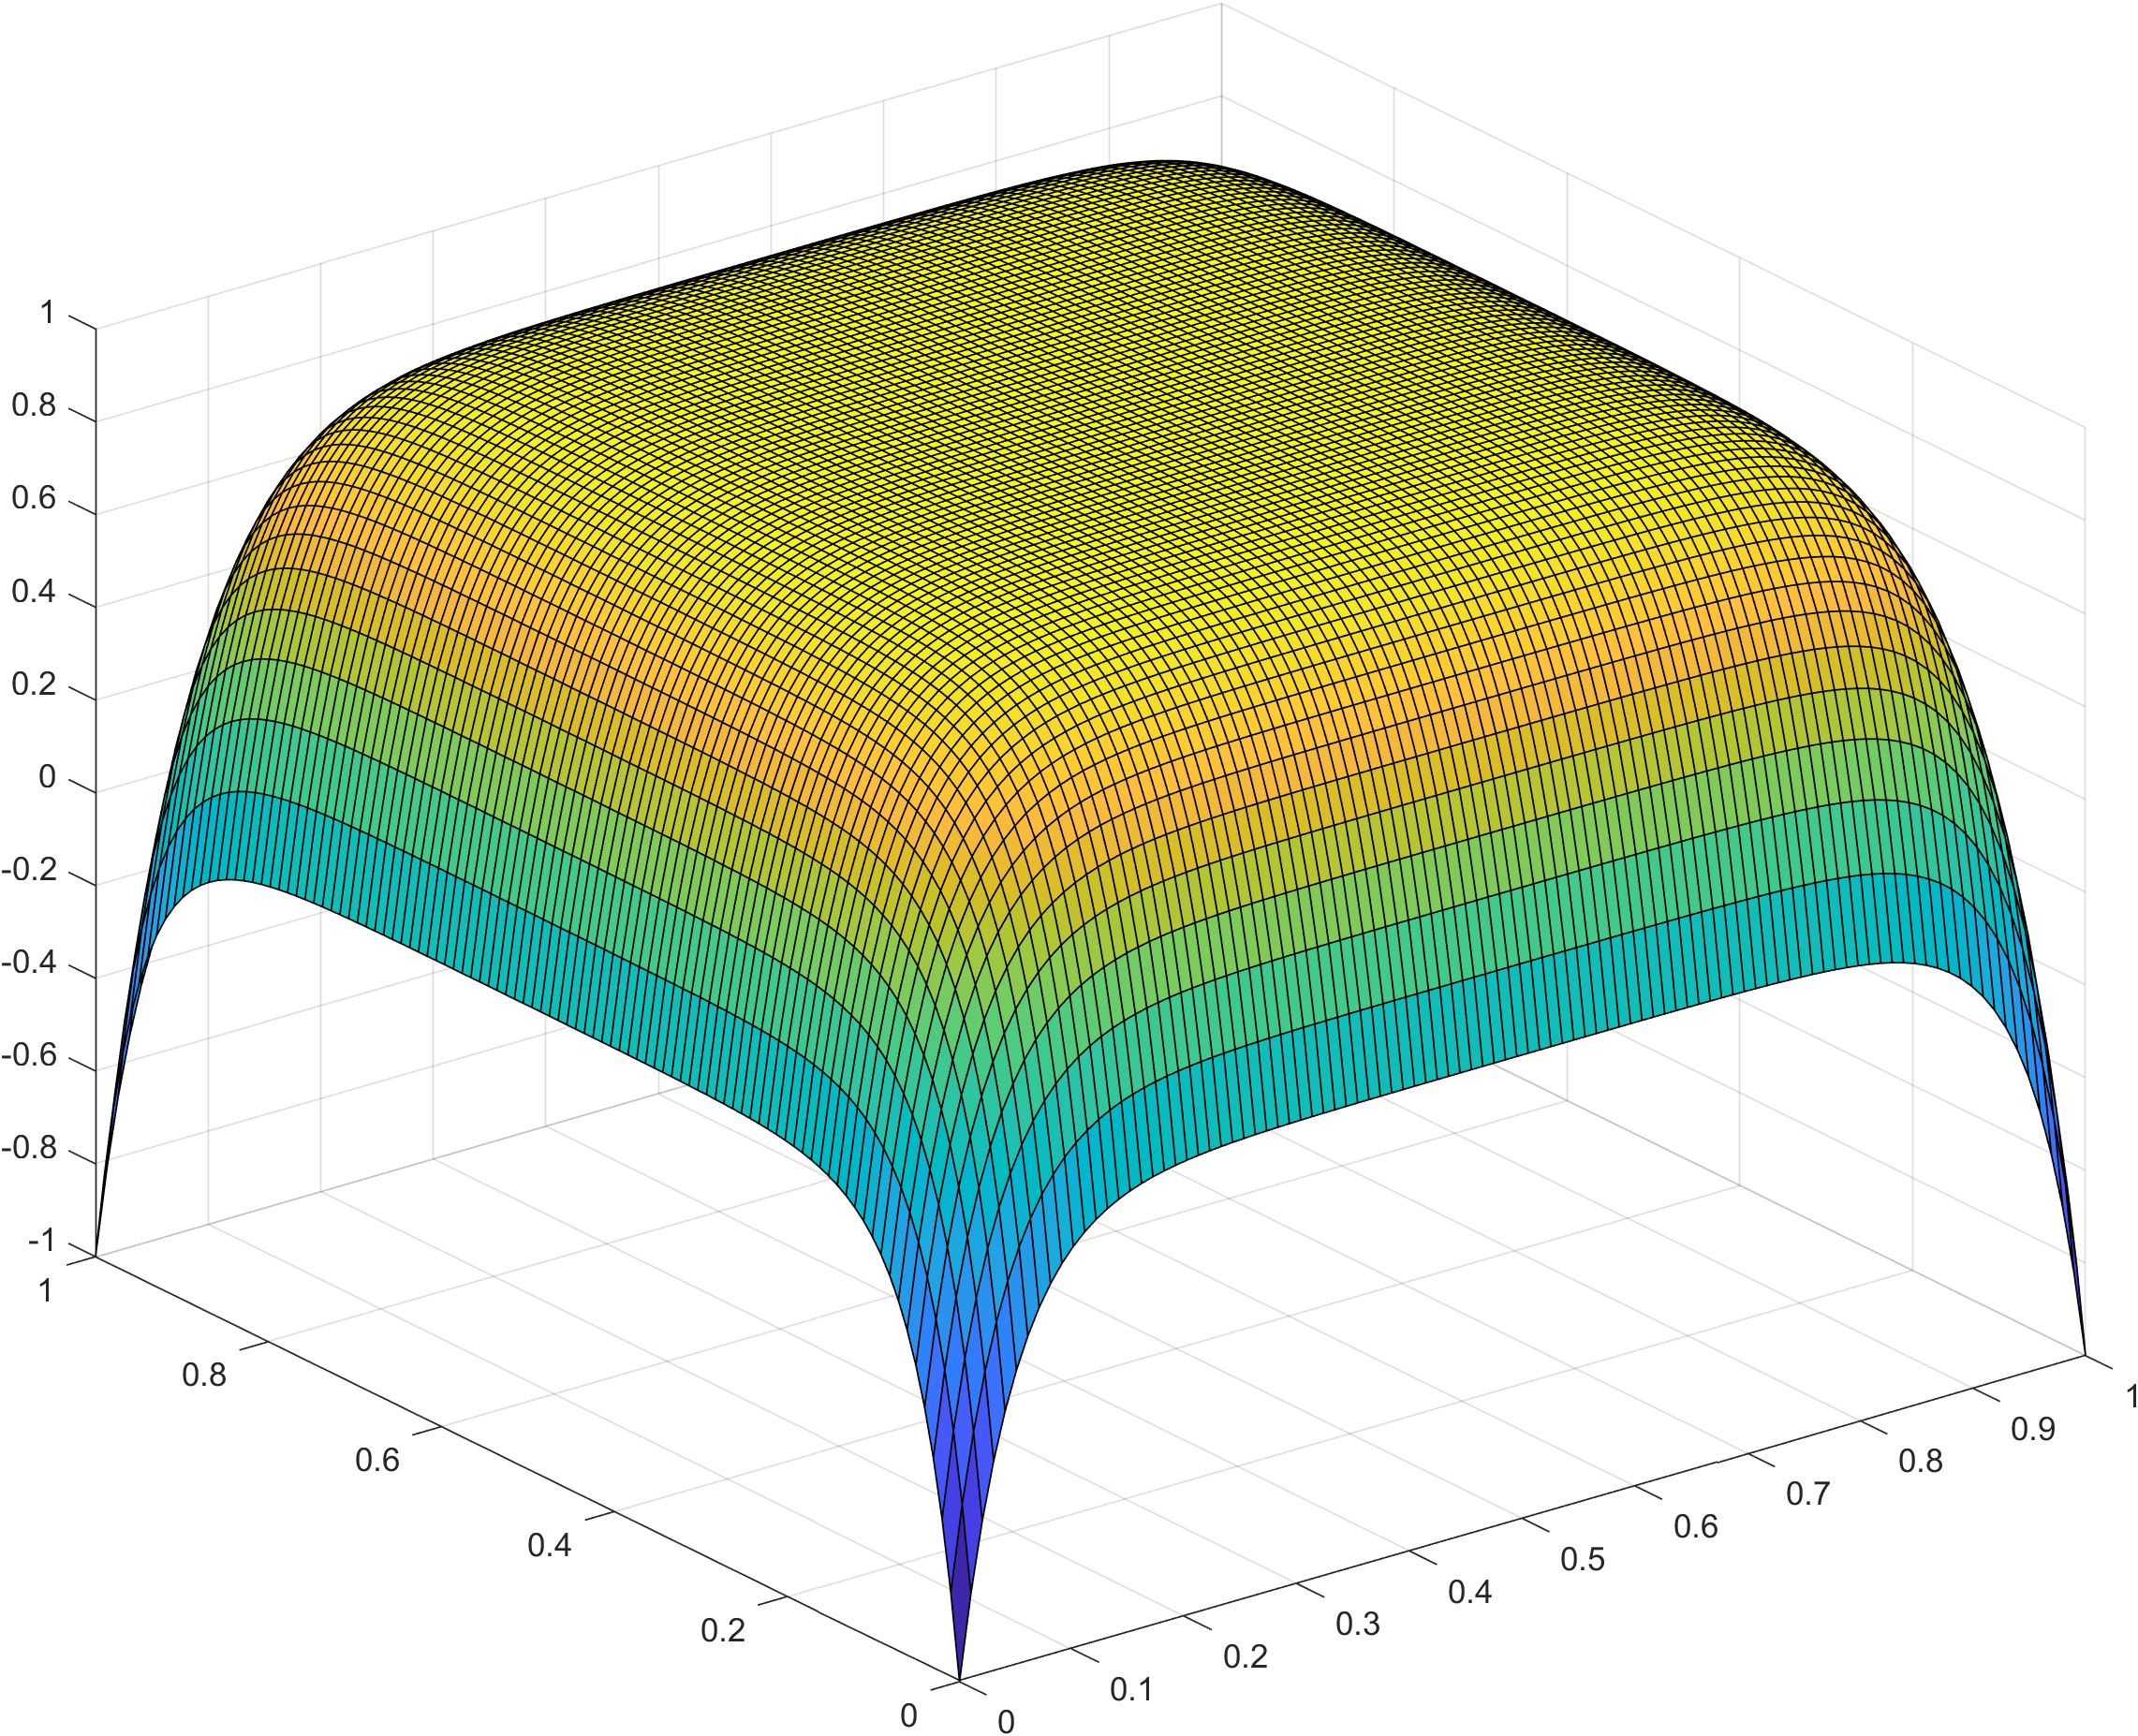
\includegraphics[height=\dimIm]{../Immagini/SDR1_SE_NPunti=100.png}
                            \caption{Soluzione esatta.}
                            \label{figSDR1TriangolazioniEsatta}
                        \end{subfigure}
                        \begin{subfigure}[t]{\lungSF}
                            \centering
                            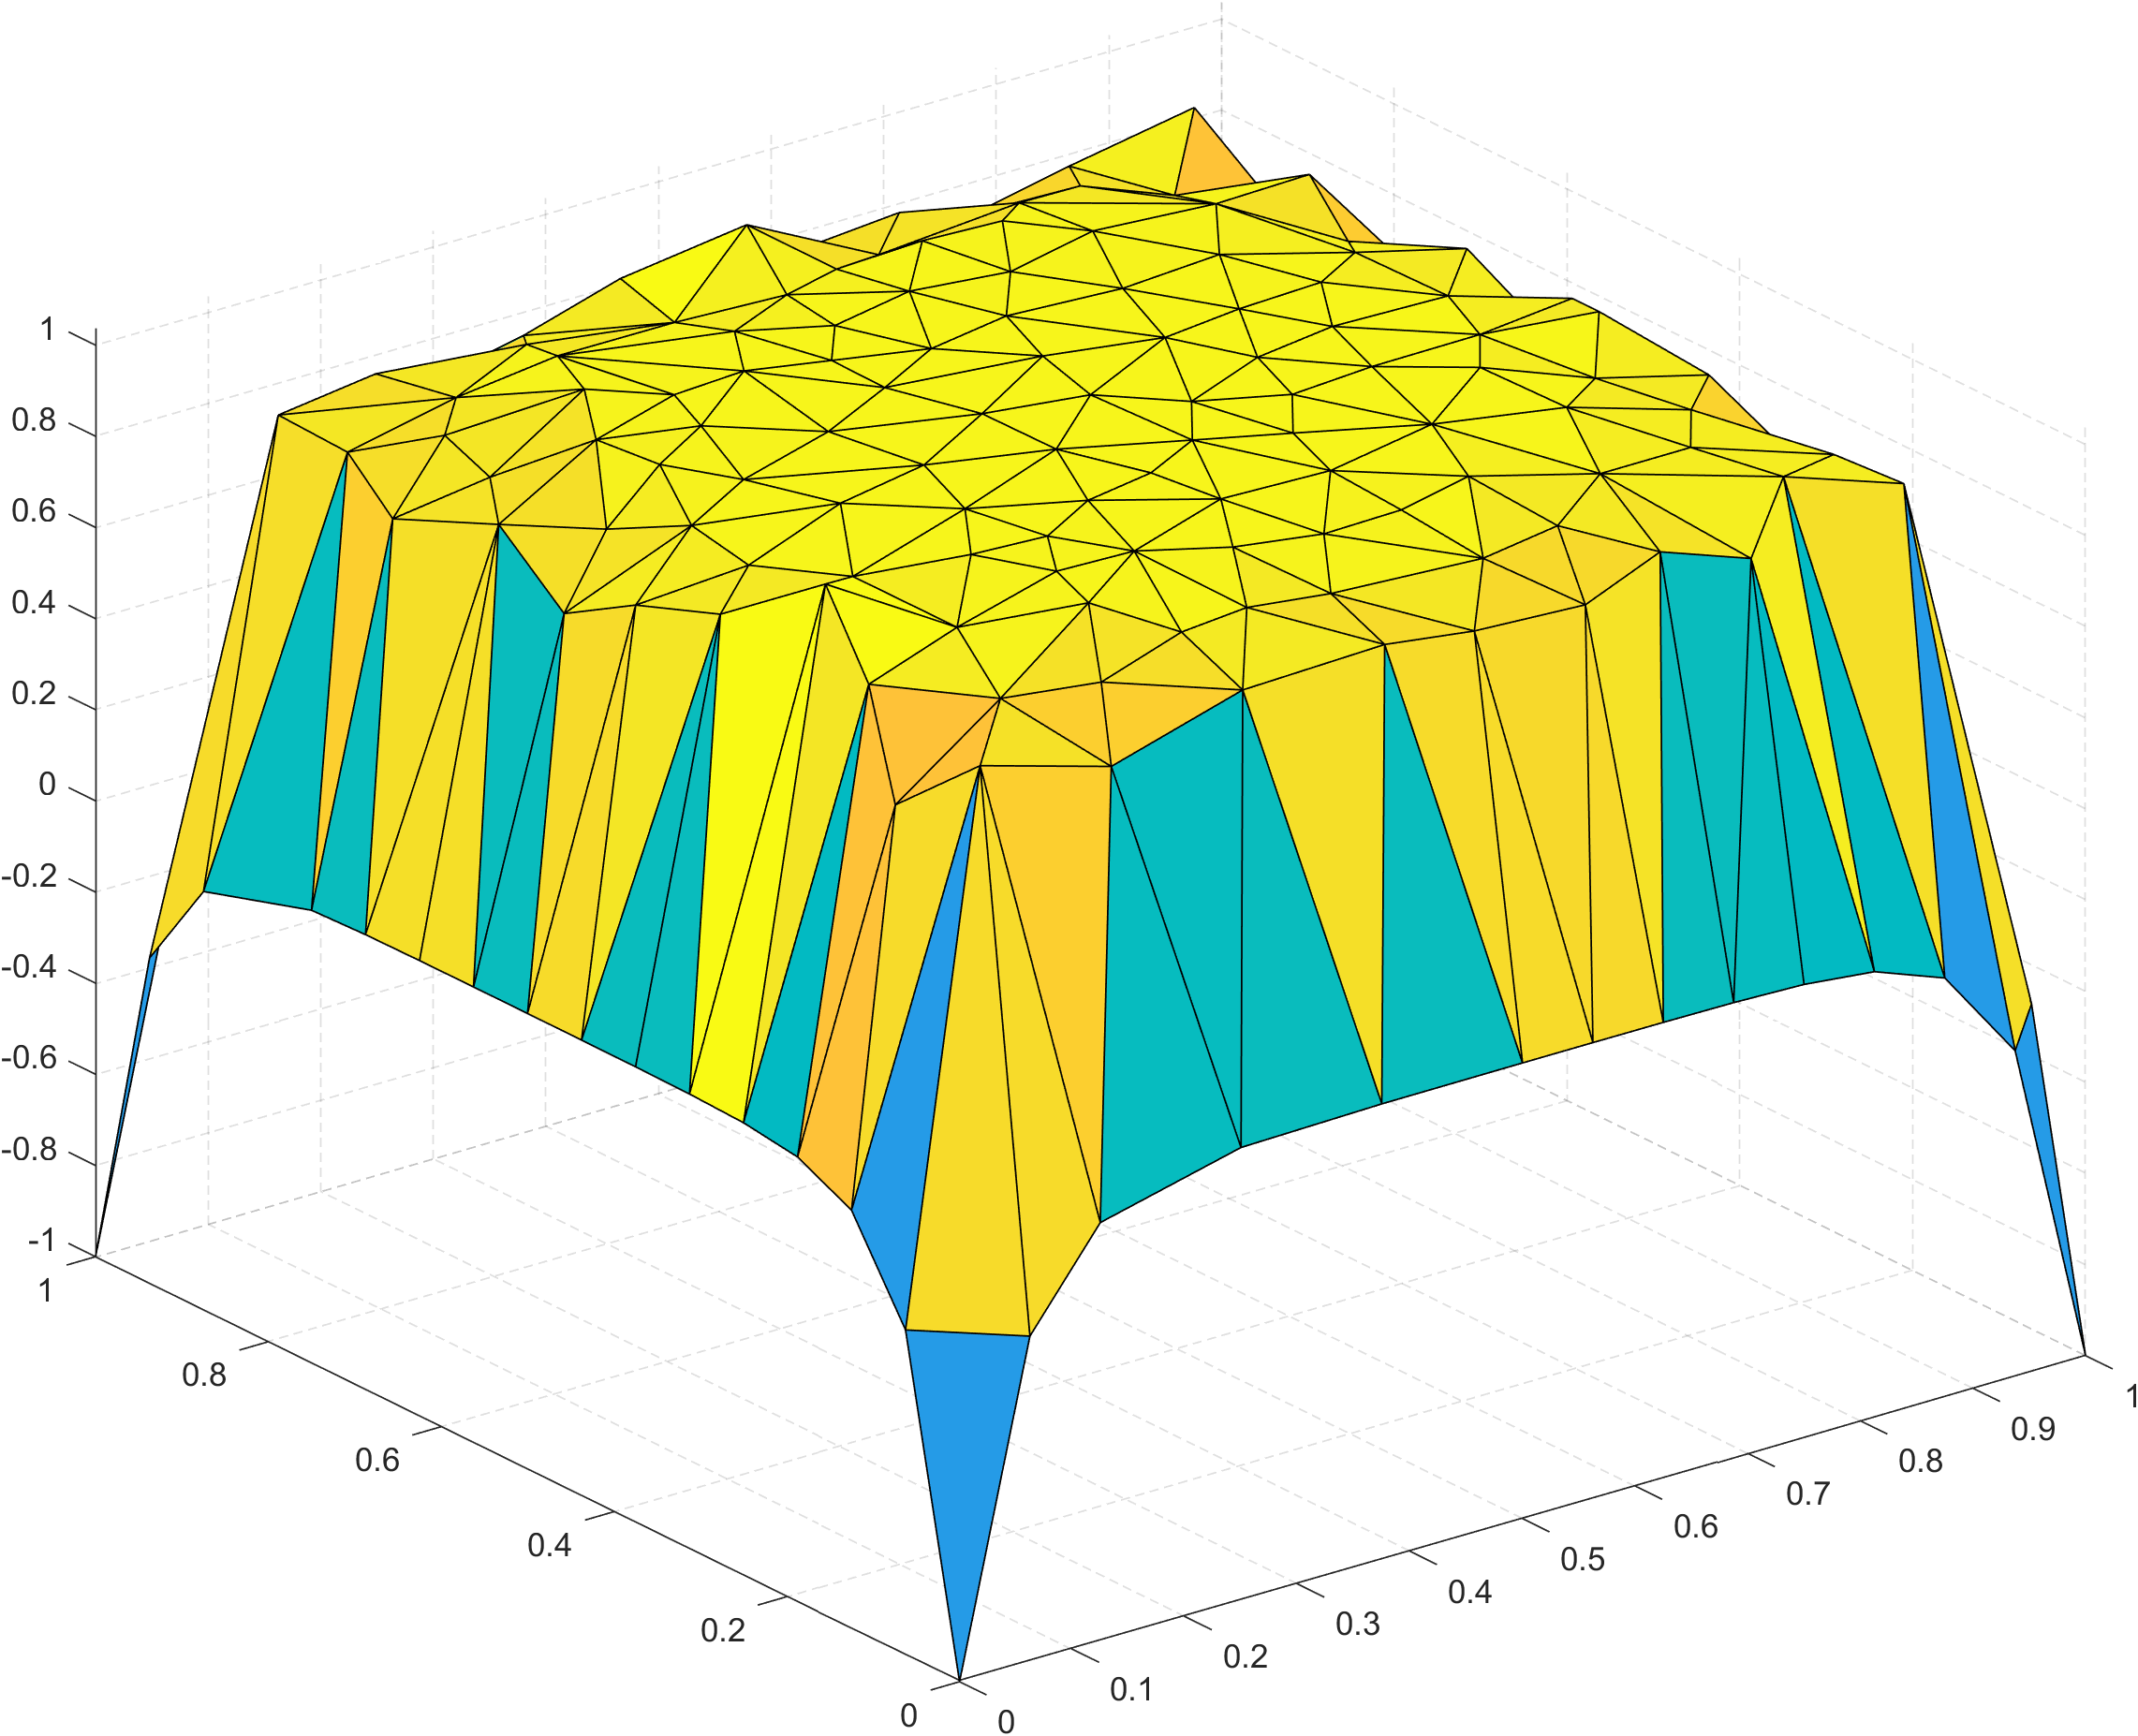
\includegraphics[height=\dimIm]{../Immagini/SDR1_SA_P1_AMax=0.005.png}
                            \caption{Soluzione qualitativa senza \textit{ML}.}
                            \label{figSDR1TriangolazioniP1SA}
                        \end{subfigure}
                        \begin{subfigure}[t]{\lungSF}
                            \centering
                            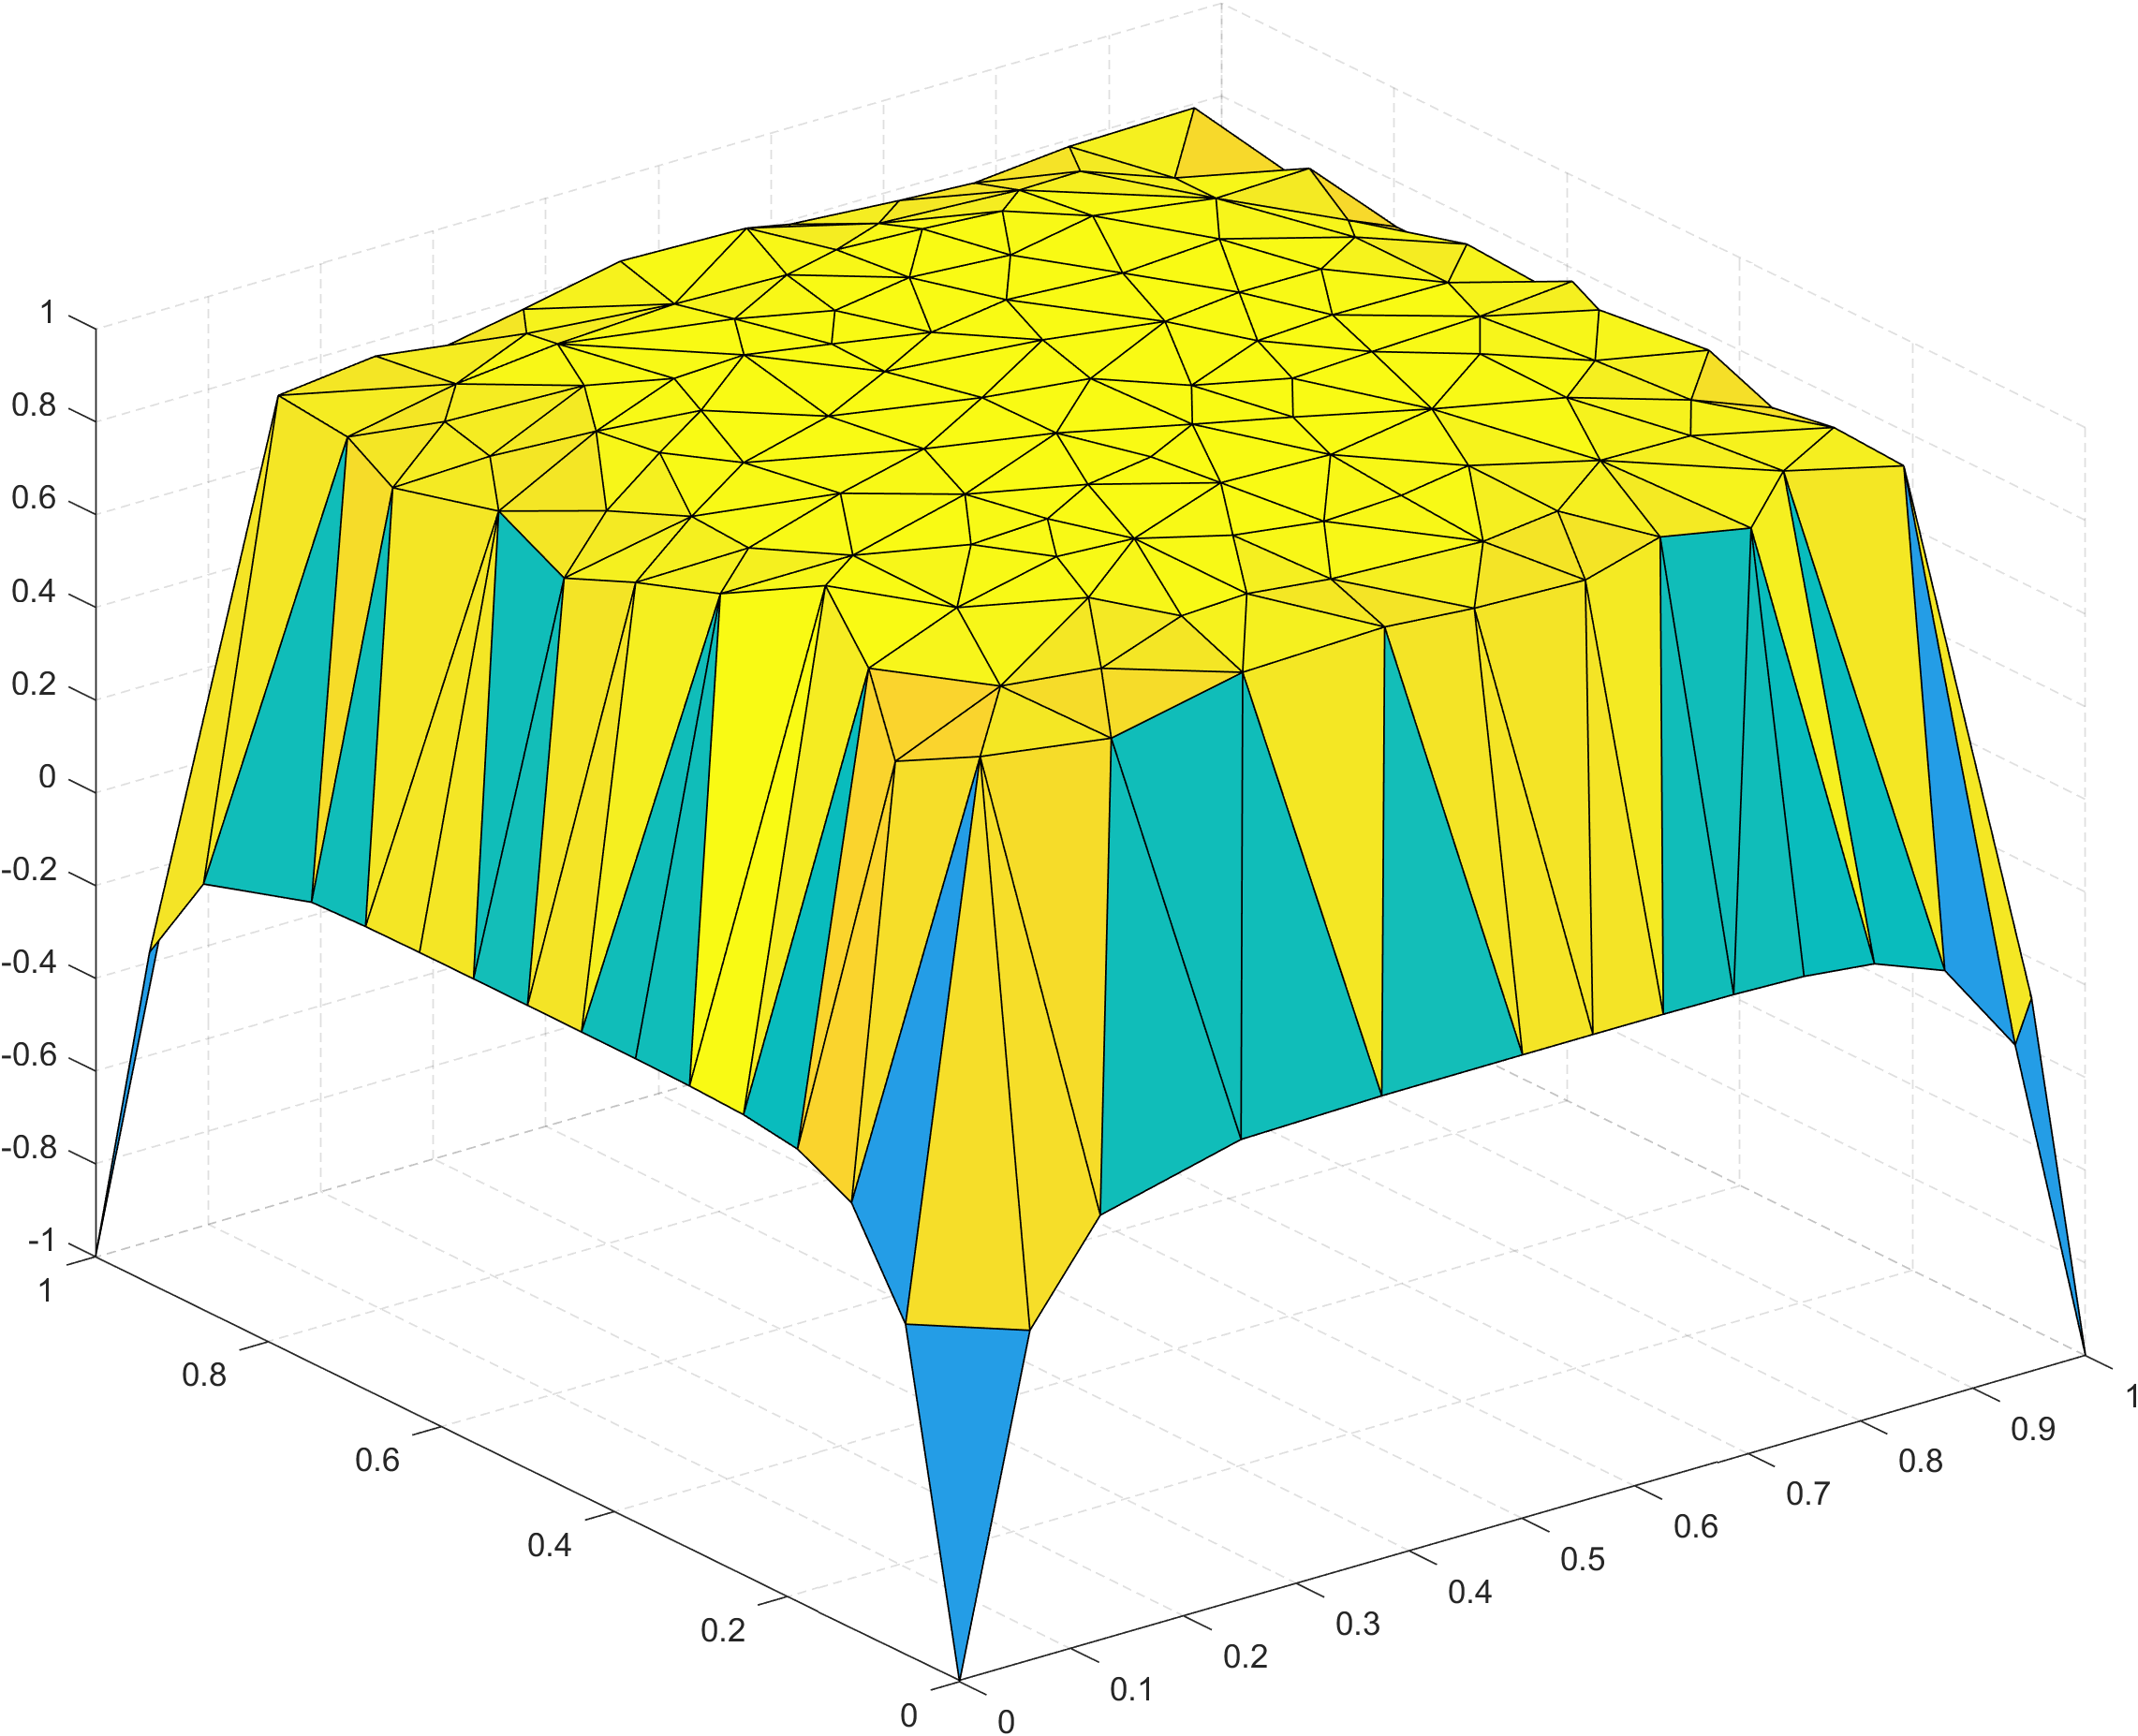
\includegraphics[height=\dimIm]{../Immagini/SDR1_CA_P1_AMax=0.005.png}
                            \caption{Soluzione qualitativa con \textit{ML}.}
                            \label{figSDR1TriangolazioniP1CA}
                        \end{subfigure}
                    }
                    \distR
        
                    \renewcommand{\lungSF}{.5\linewidth}
                    \renewcommand{\dimIm}{\linewidth}
                    \newcommand{\distC}{\hspace{7.5pt}} % Distanza tra le colonne
                    \makebox[\linewidth][c]{
                        \begin{subfigure}[t]{\lungSF}
                            \centering
                            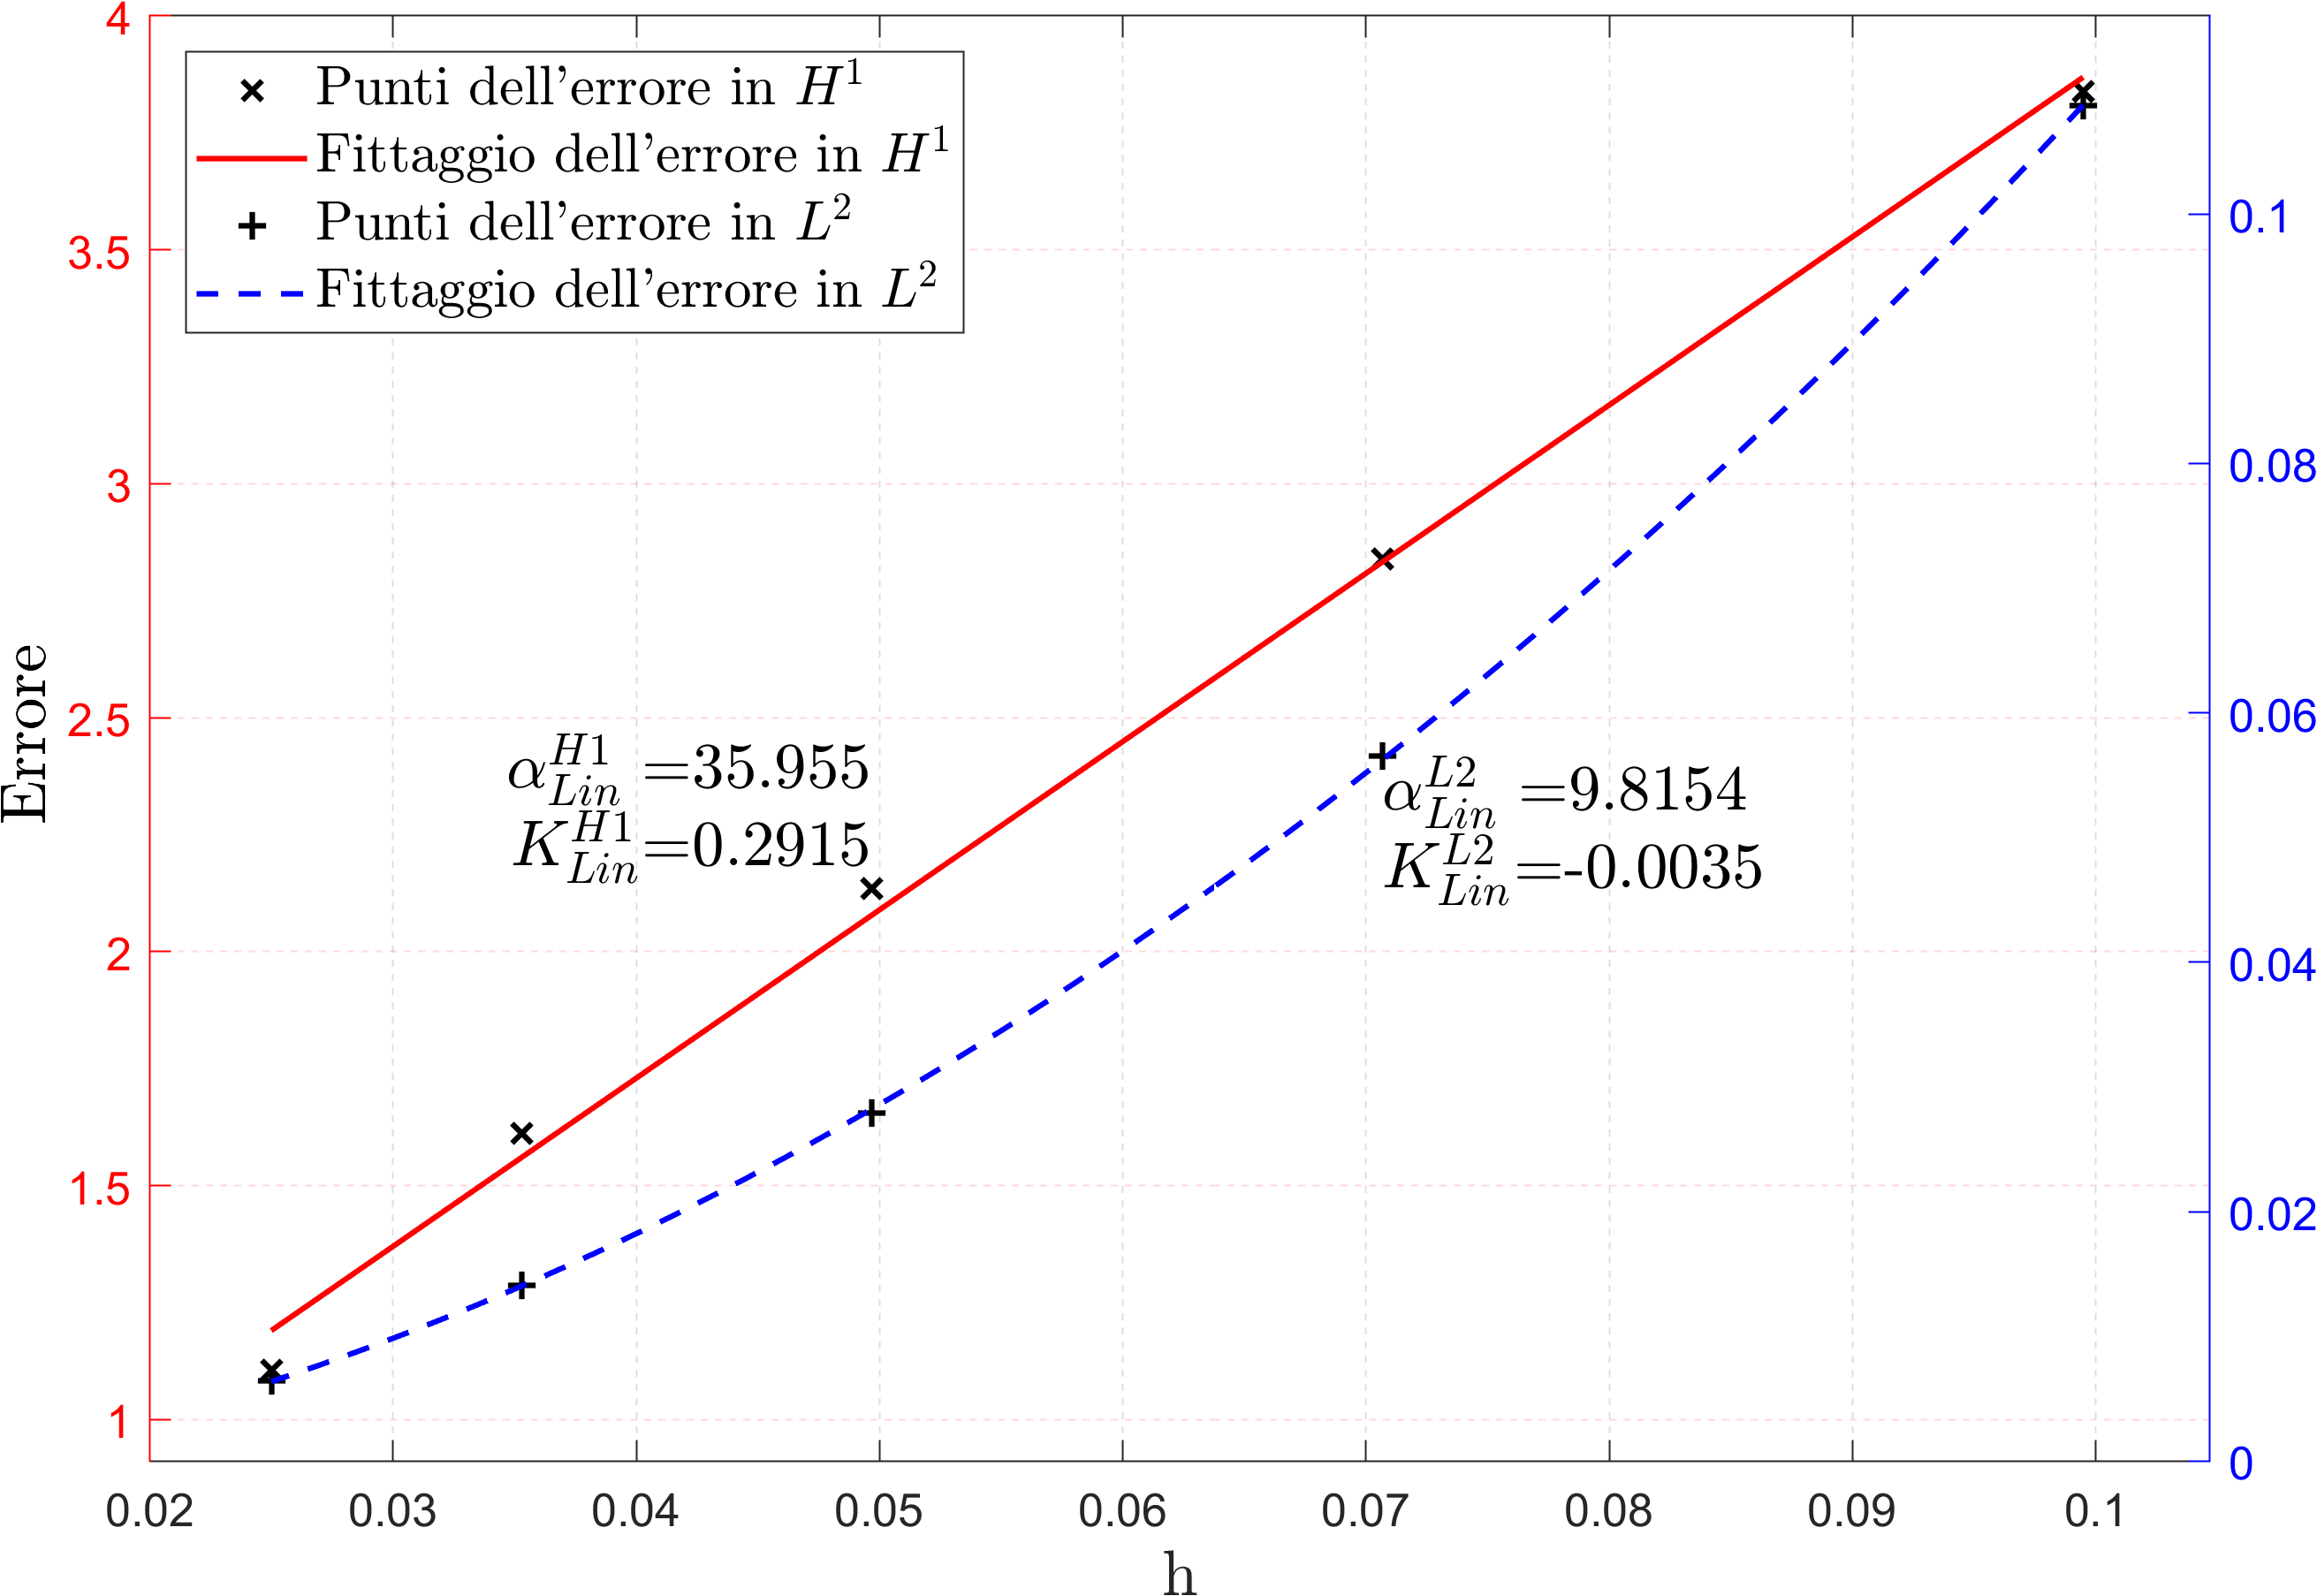
\includegraphics[width=\dimIm]{../Immagini/SDR1_P1_SA_ErrLin_AMax=0.01_NSim=5.png}
                        \caption{Errore in scala lineare senza \textit{ML}.}
                        \label{figSDR1ErroreP1LinSA}
                        \end{subfigure}
                        \distC
                        \begin{subfigure}[t]{\lungSF}
                            \centering
                            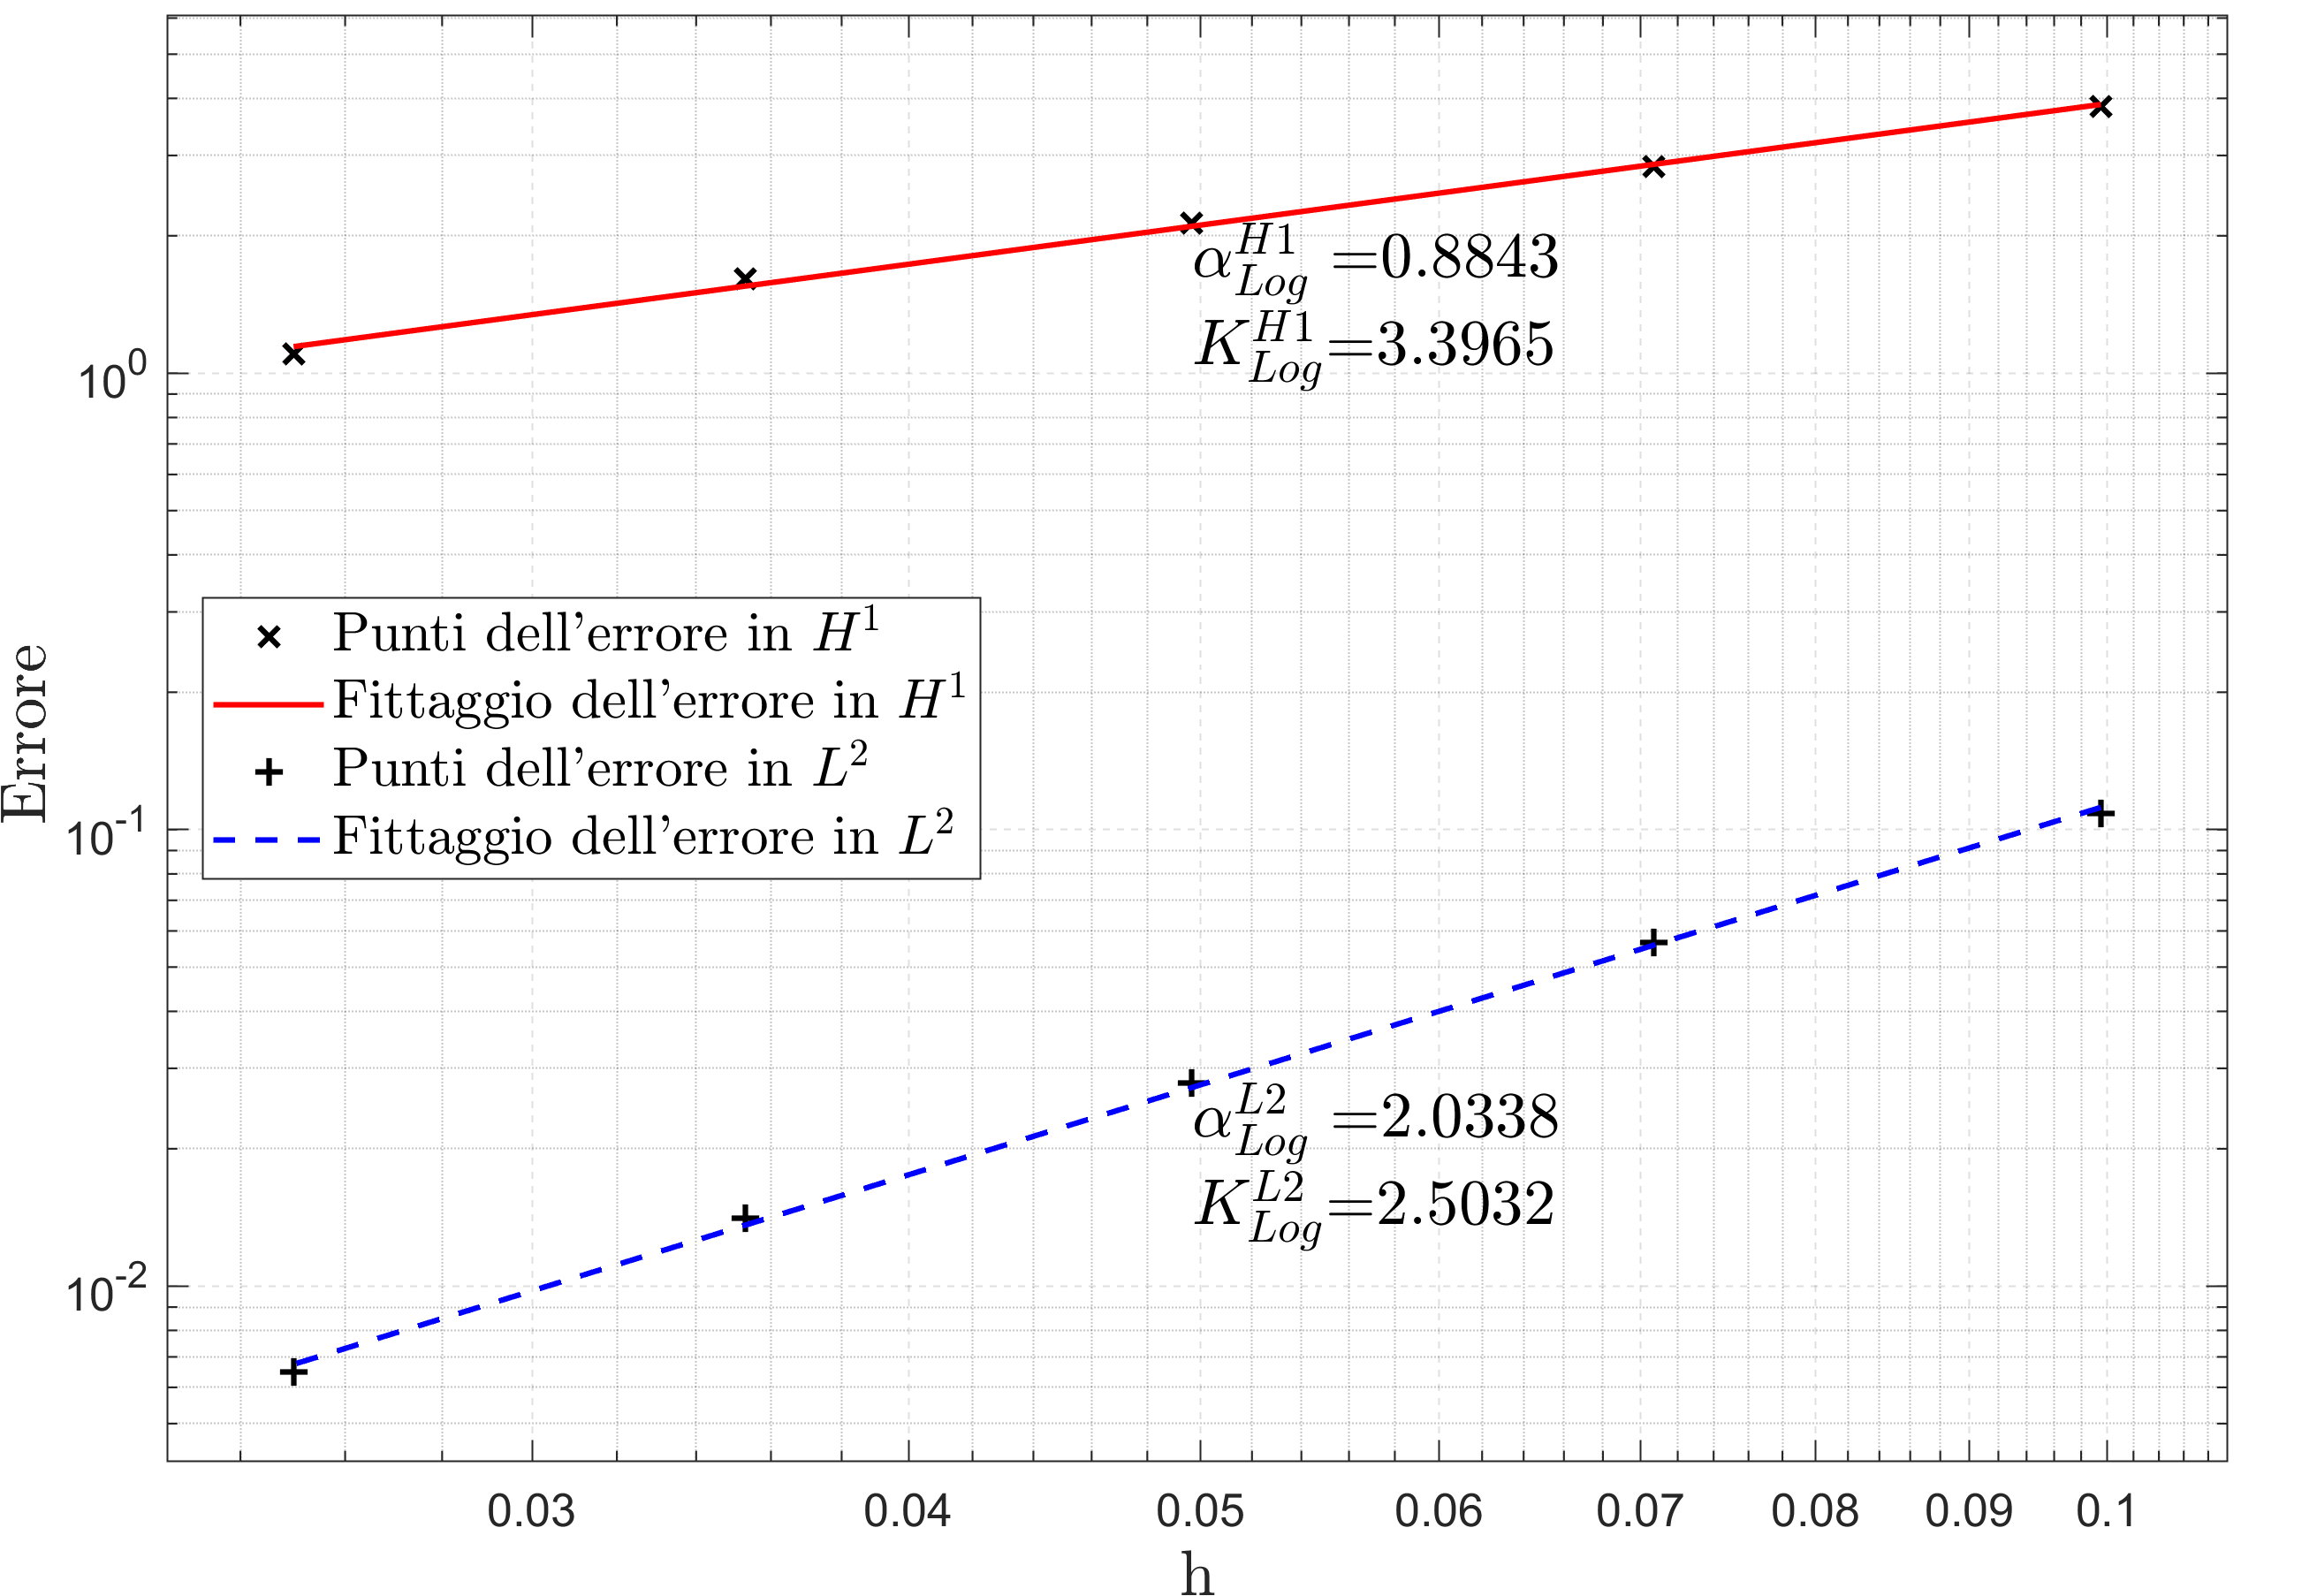
\includegraphics[width=\dimIm]{../Immagini/SDR1_P1_SA_ErrLog_AMax=0.01_NSim=5.png}
                        \caption{Errore in scala logaritmica senza \textit{ML}.}
                        \label{figSDR1ErroreP1LogSA}
                        \end{subfigure}
                    }
                    \distR
        
                    \makebox[\linewidth][c]{
                        \begin{subfigure}[t]{\lungSF}
                            \centering
                            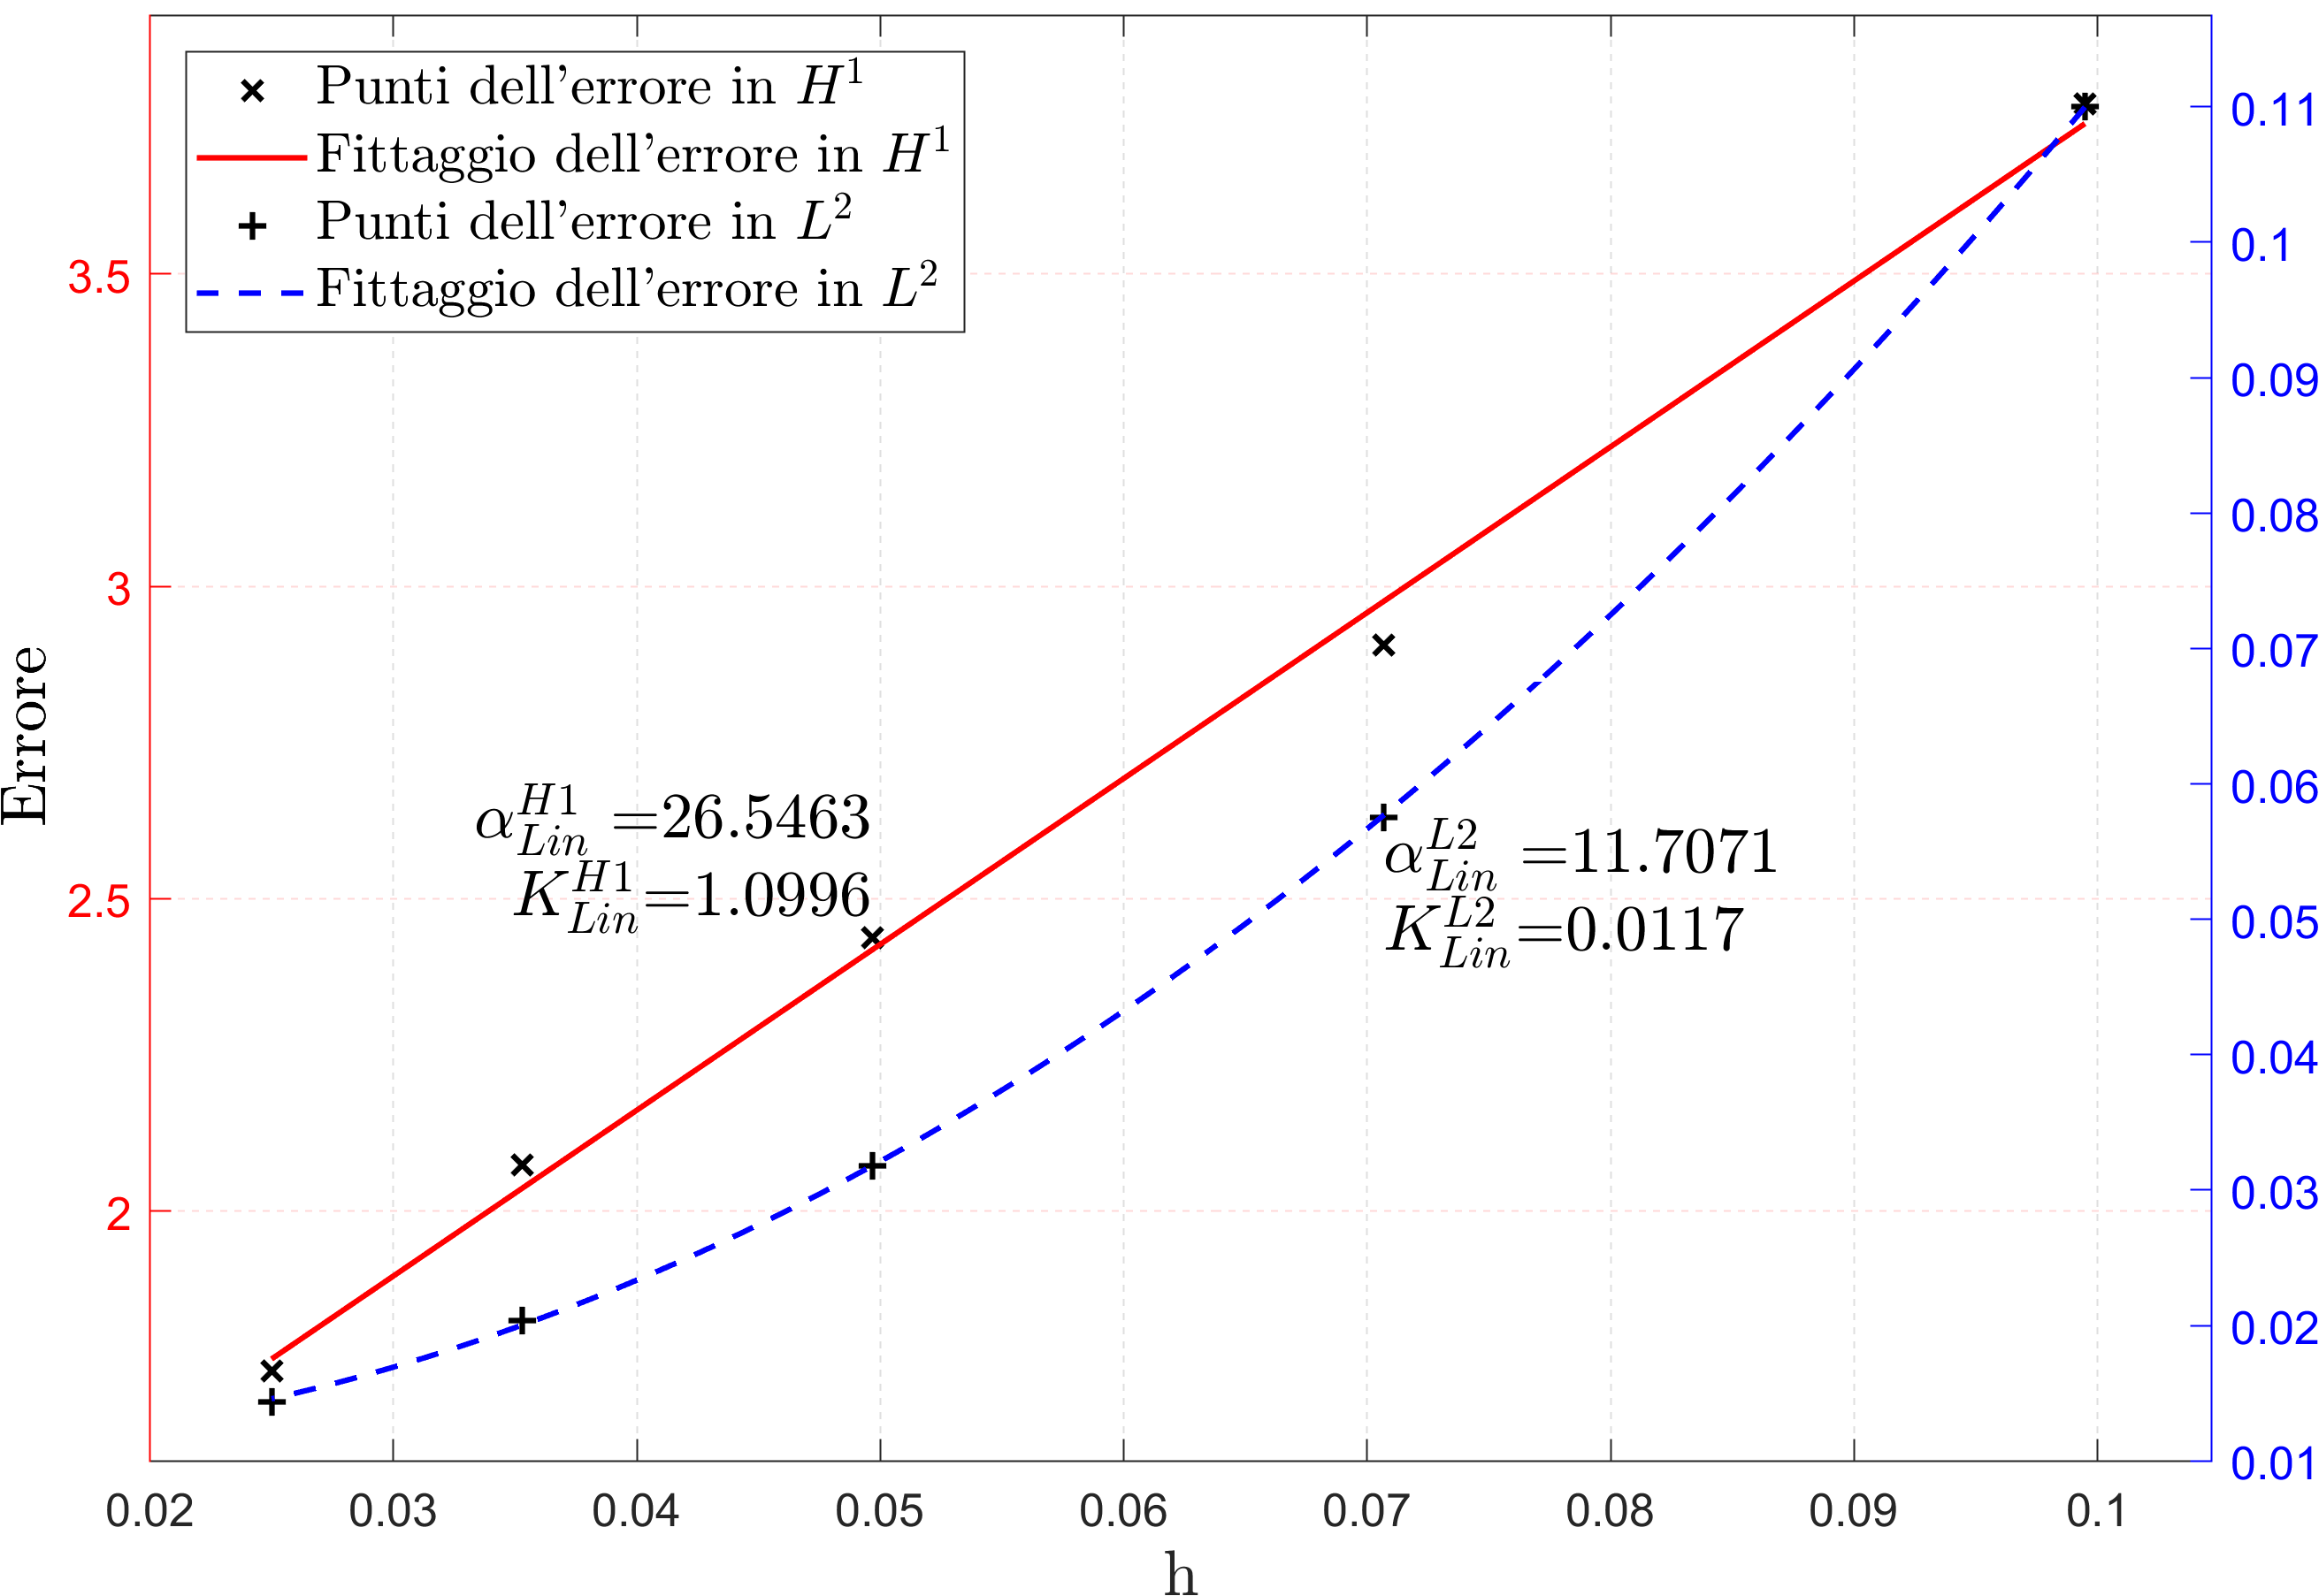
\includegraphics[width=\dimIm]{../Immagini/SDR1_P1_CA_ErrLin_AMax=0.01_NSim=5.png}
                        \caption{Errore in scala lineare con \textit{ML}.}
                        \label{figSDR1ErroreP1LinCA}
                        \end{subfigure}
                        \distC
                        \begin{subfigure}[t]{\lungSF}
                            \centering
                            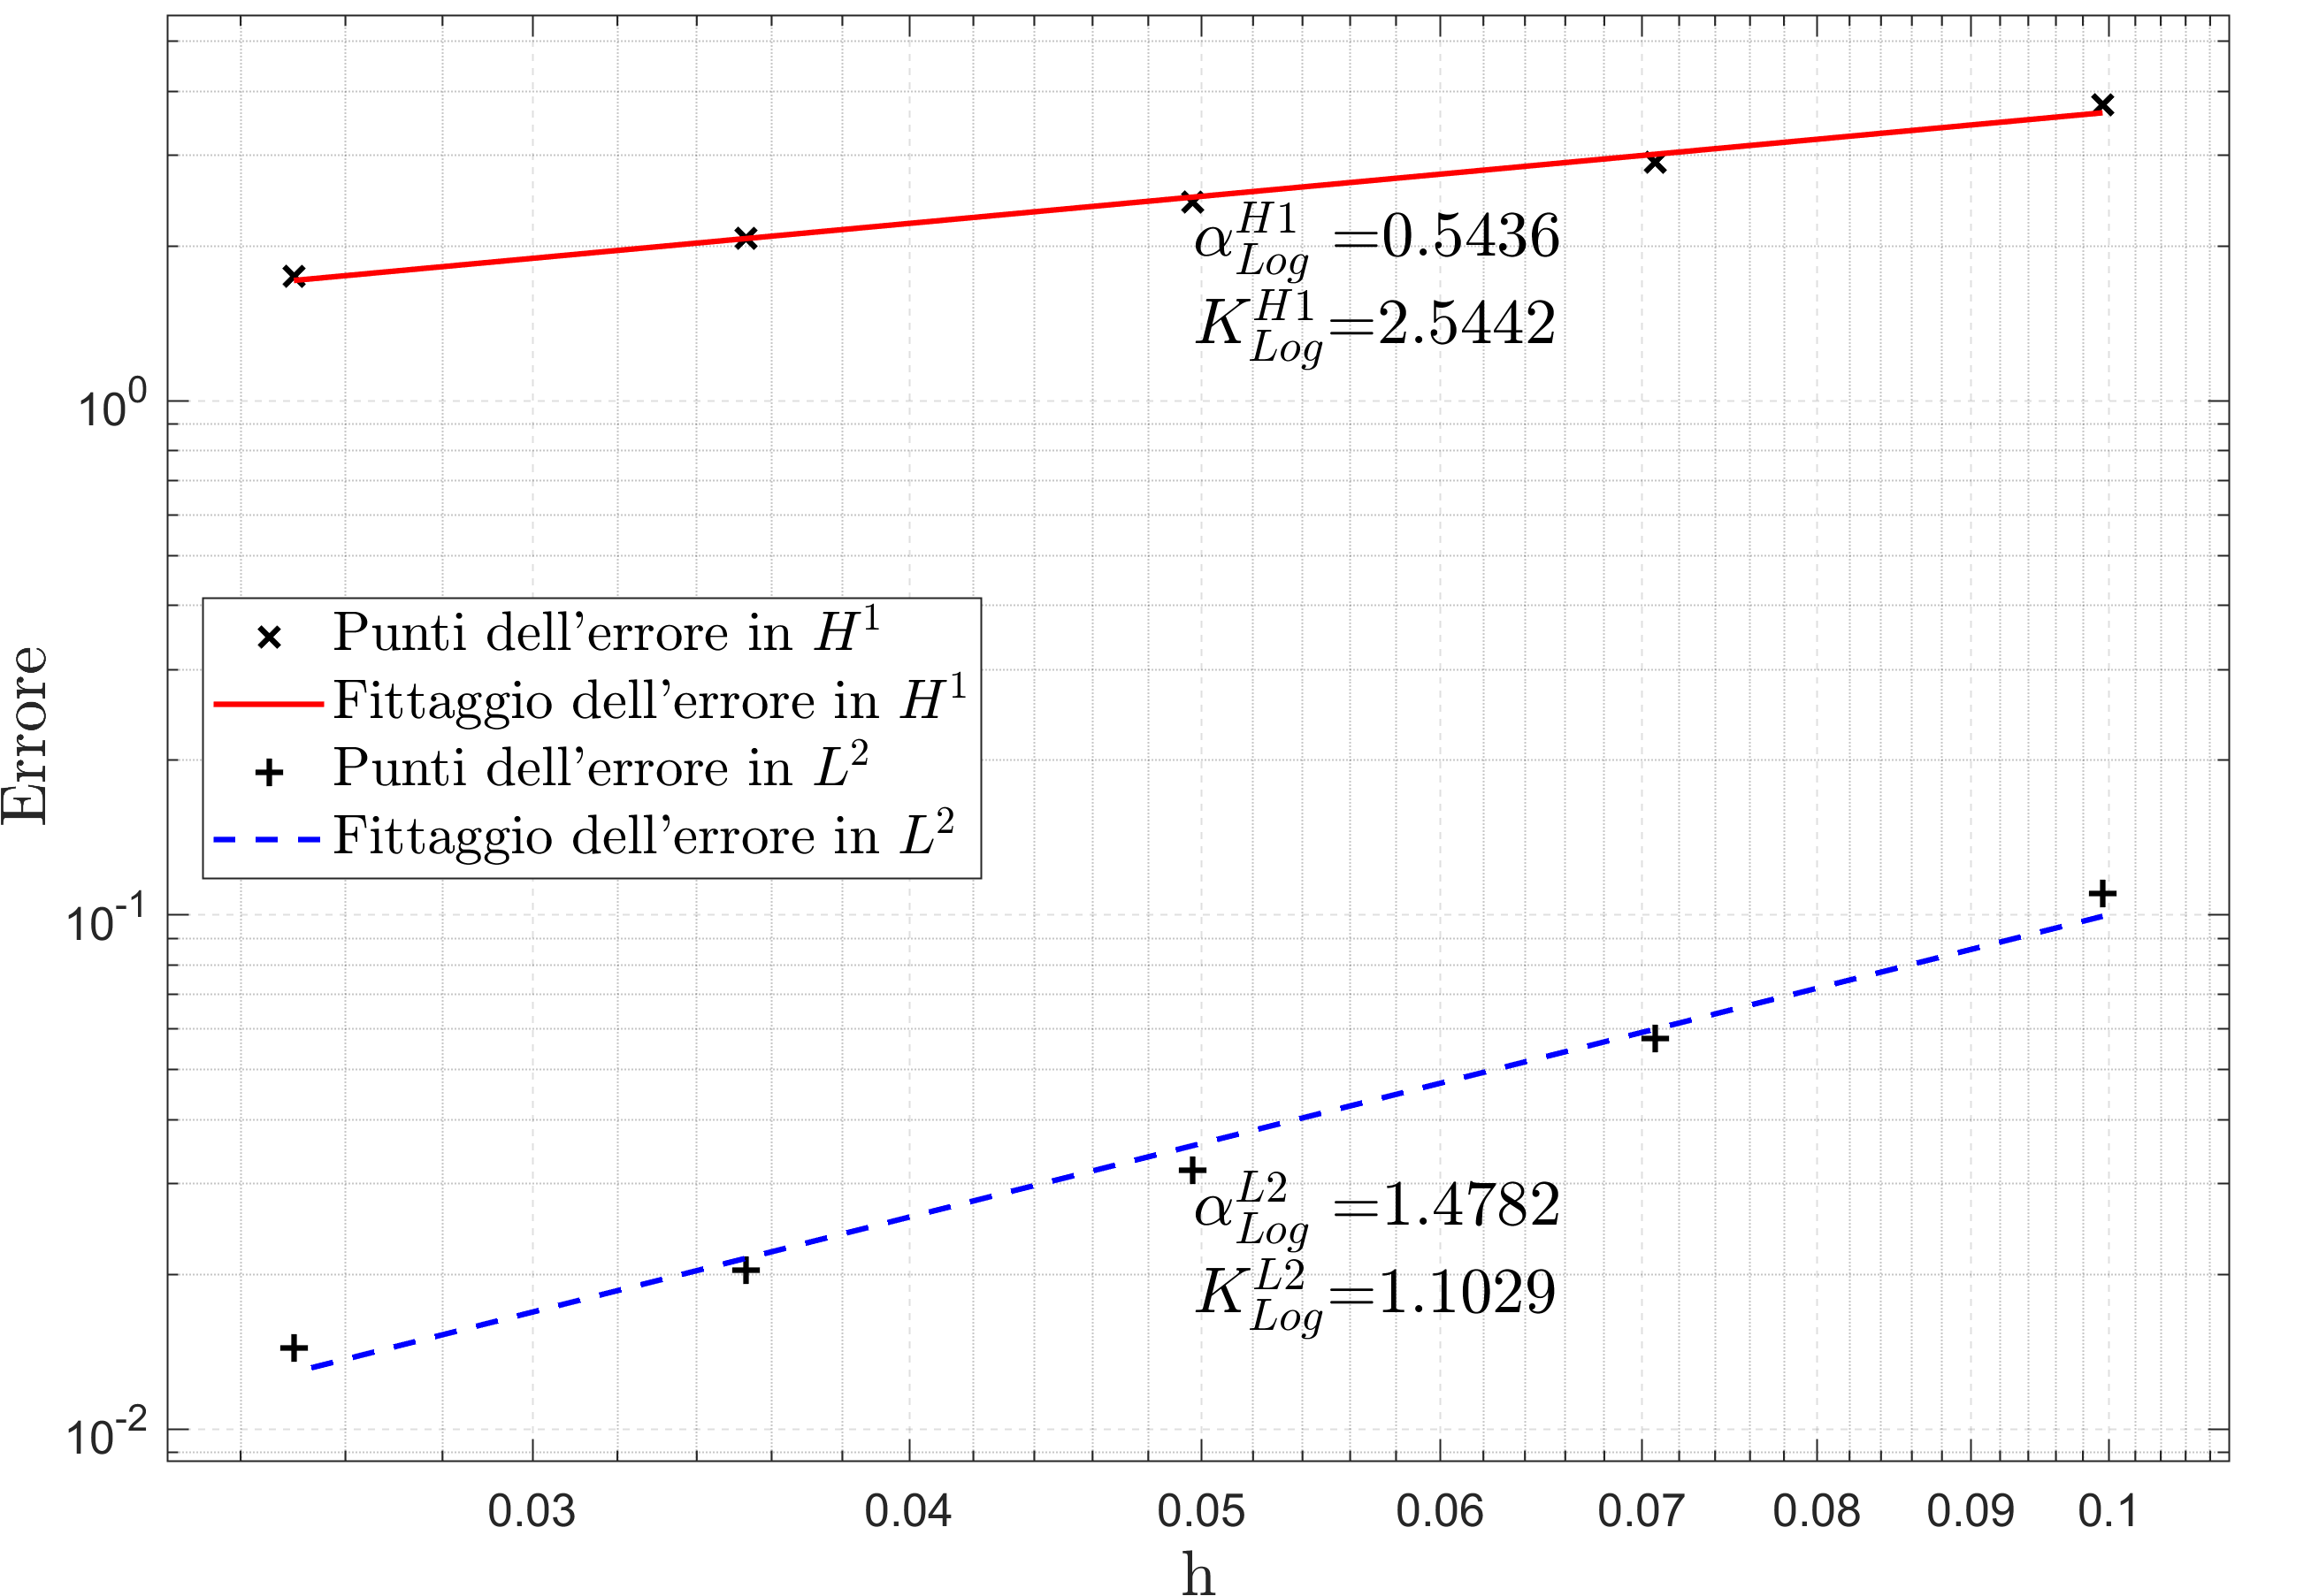
\includegraphics[width=\dimIm]{../Immagini/SDR1_P1_CA_ErrLog_AMax=0.01_NSim=5.png}
                        \caption{Errore in scala logaritmica con \textit{ML}.}
                        \label{figSDR1ErroreP1LogCA}
                        \end{subfigure}
                    }
                    \caption{Nelle Figg. \ref{figSDR1TriangolazioniEsatta}-\ref{figSDR1TriangolazioniP1CA} sono mostrate le soluzioni dell'SDR1: una esatta e le altre approssimate, coi $\mathbb{P}_1$, con e senza ammassamento; invece nelle \ref{figSDR1ErroreP1LinSA}-\ref{figSDR1ErroreP1LogCA} sono illustrati in due scale diverse gli errori in norma $H^1$ ed $L^2$, coi $\mathbb{P}_1$, con e senza ammassamento. I parametri dati a \textit{BBTR} sono spiegati nel $\S$\ref{parPremessaParametriBBTR}.}
                    \label{figSDR1}
                \end{figure*}
    
                \begin{figure*}[p]
                    \newcommand{\distR}{\vspace{15pt}} % Distanza tra le righe
                    
                    \newcommand{\lungSF}{0.33\textwidth}
                    \newcommand{\dimIm}{4cm}
                    \makebox[\linewidth][c]{
                        \begin{subfigure}[t]{\lungSF}
                            \centering
                            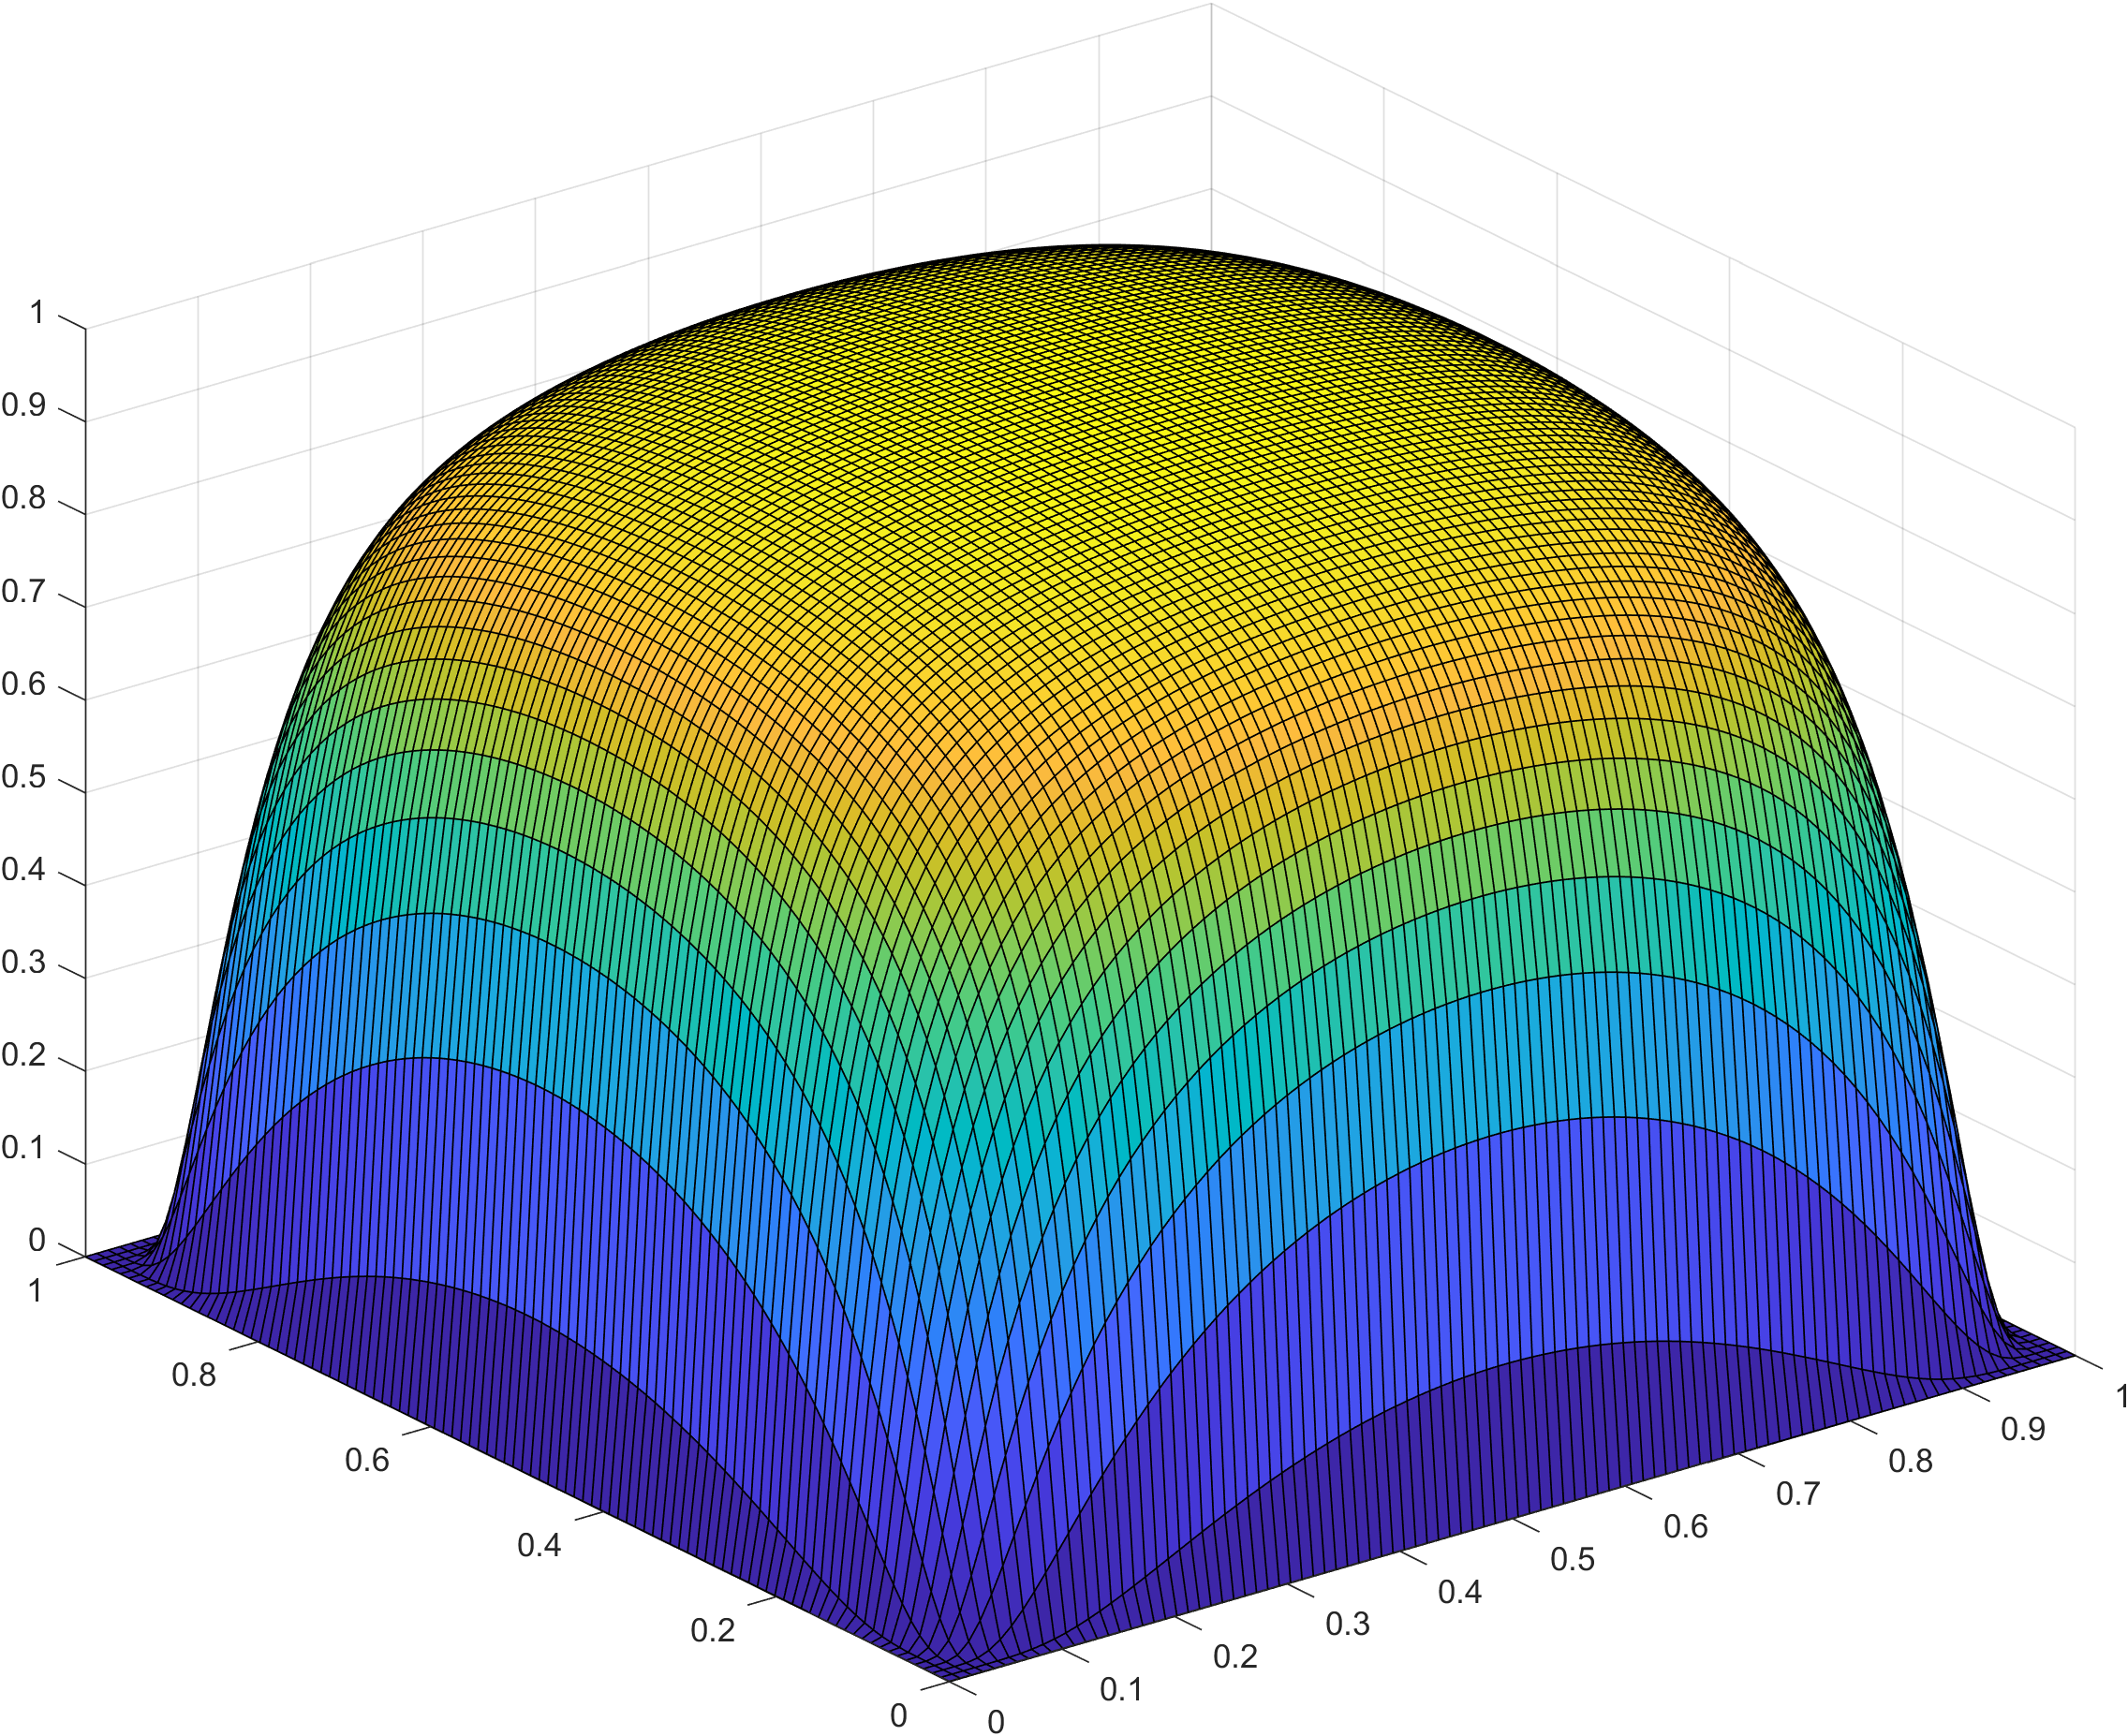
\includegraphics[height=\dimIm]{../Immagini/SDC2_SDR2_SE_NPunti=100.png}
                            \caption{Soluzione esatta.}
                            \label{figSDR2TriangolazioniEsatta}
                        \end{subfigure}
                        \begin{subfigure}[t]{\lungSF}
                            \centering
                            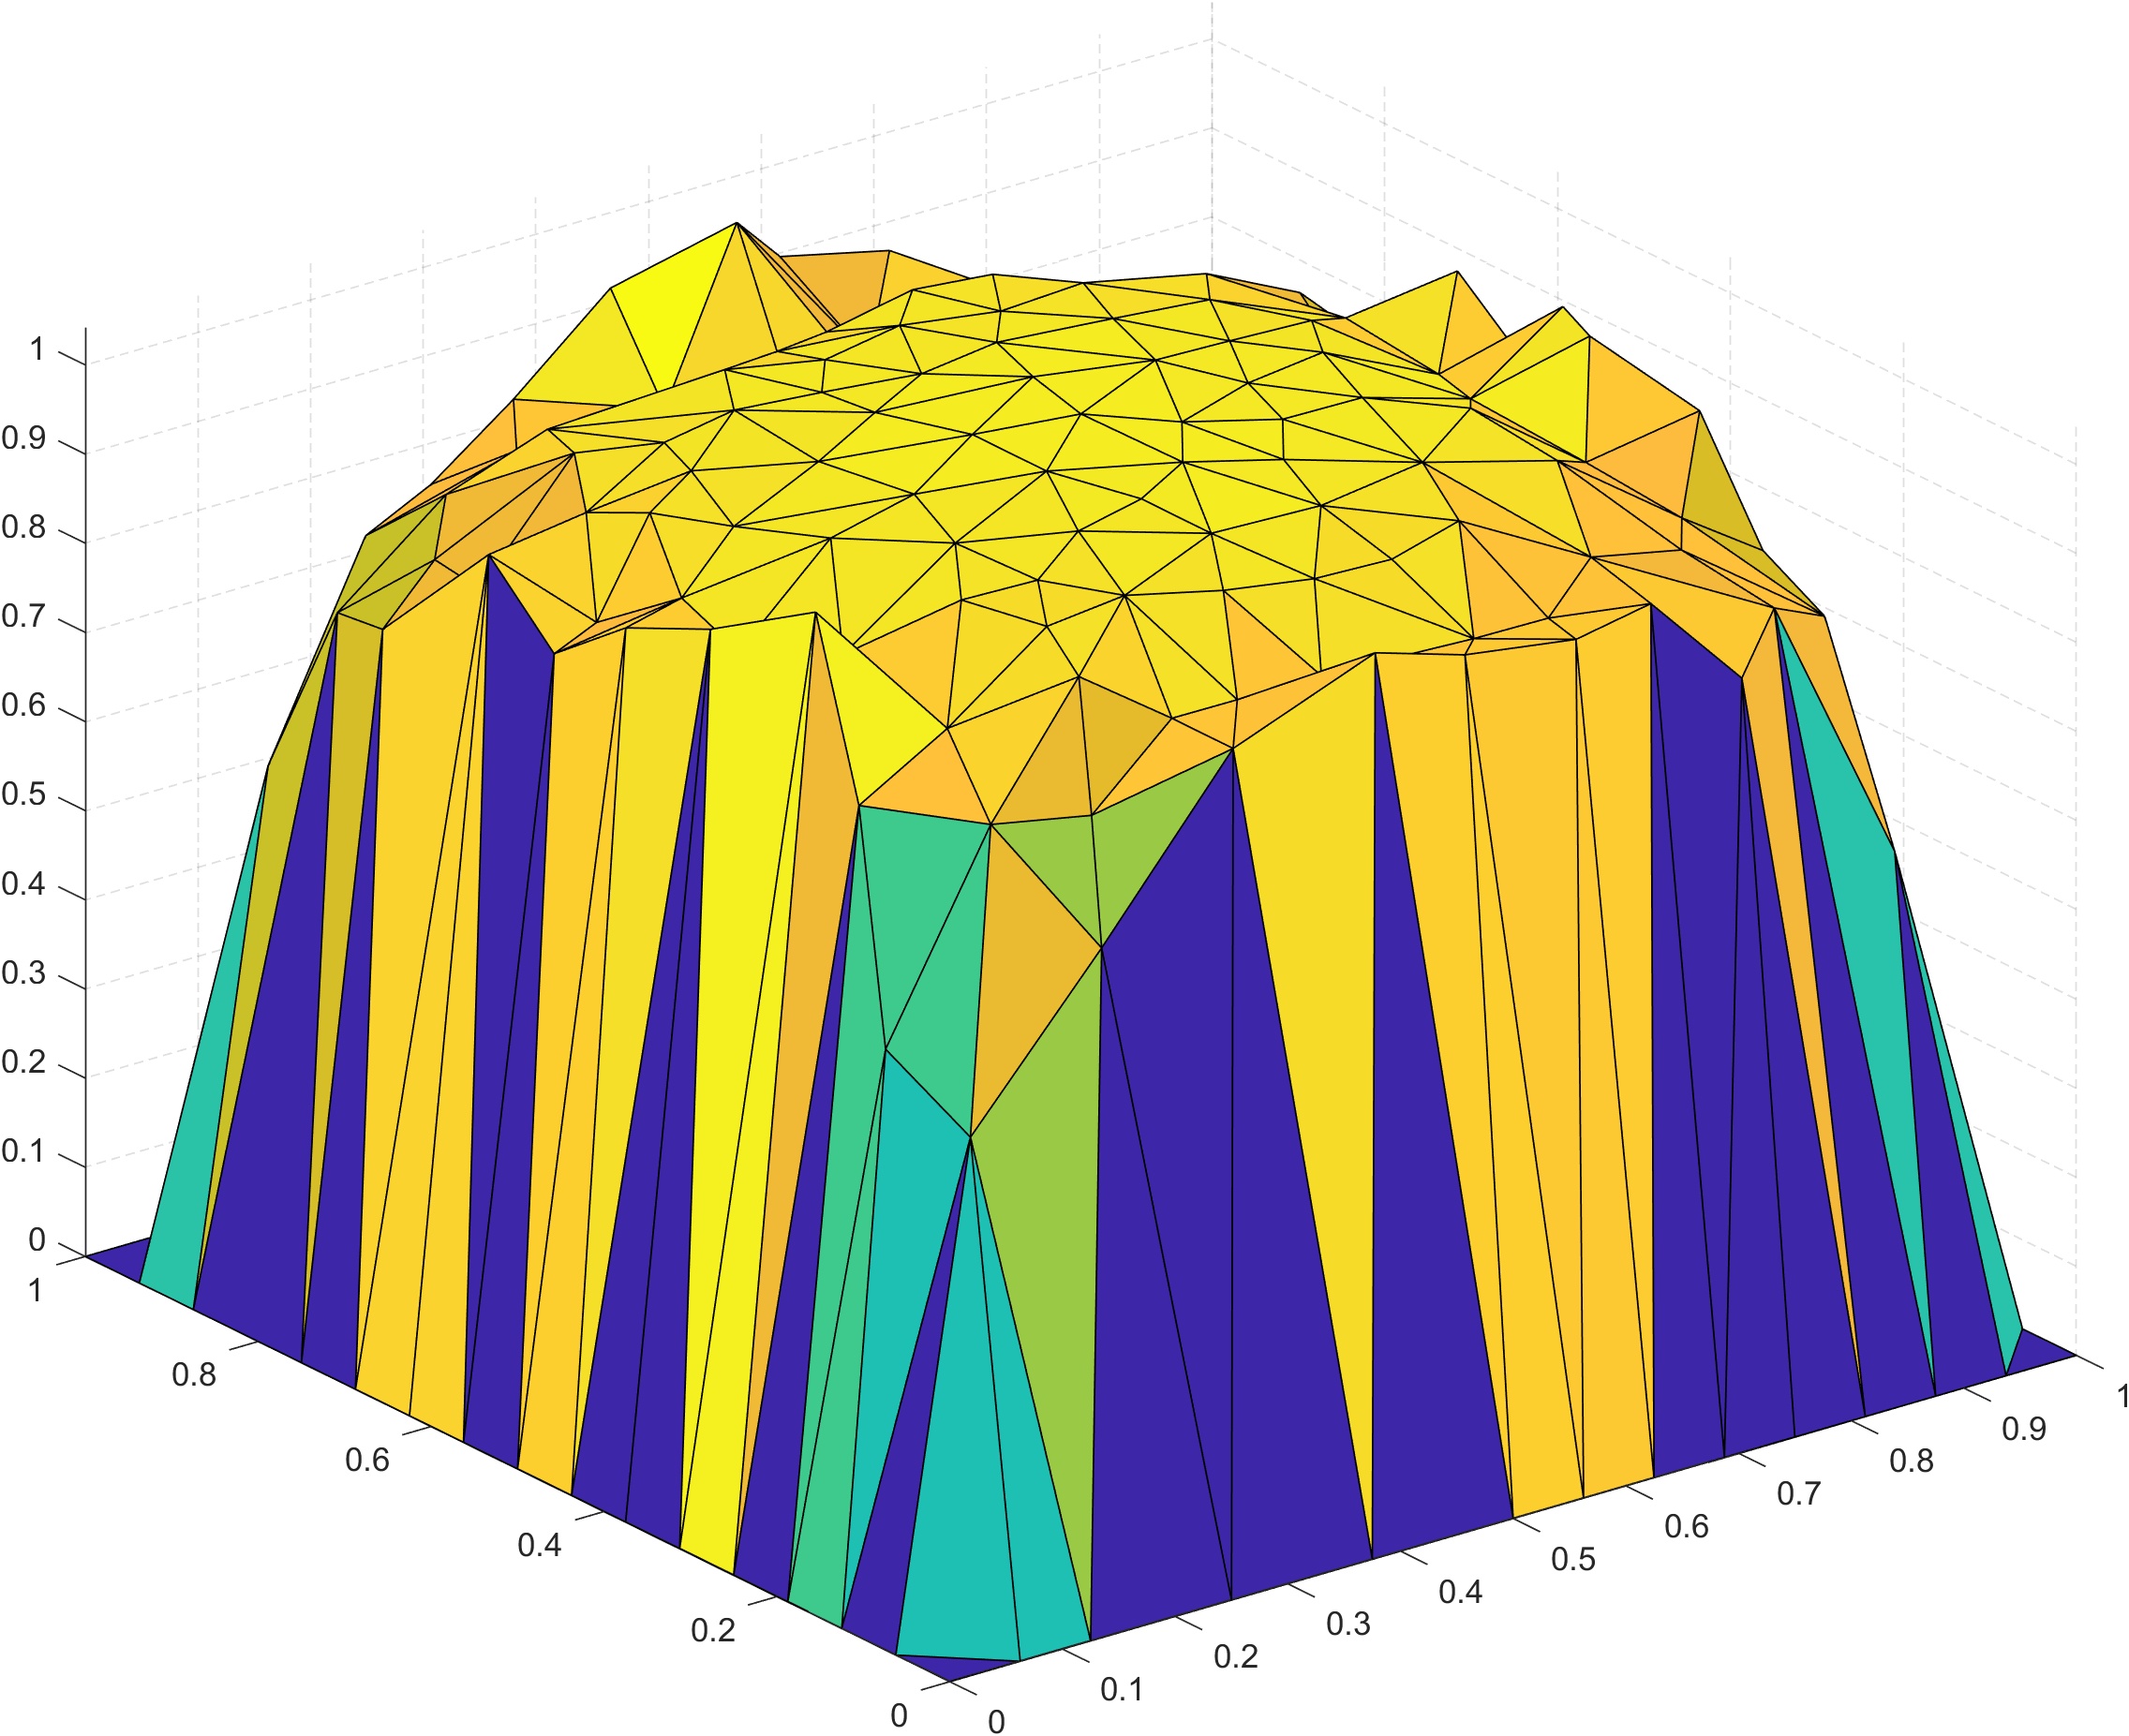
\includegraphics[height=\dimIm]{../Immagini/SDR2_SA_P1_AMax=0.005.png}
                            \caption{Soluzione qualitativa senza \textit{ML}.}
                            \label{figSDR2TriangolazioniP1SA}
                        \end{subfigure}
                        \begin{subfigure}[t]{\lungSF}
                            \centering
                            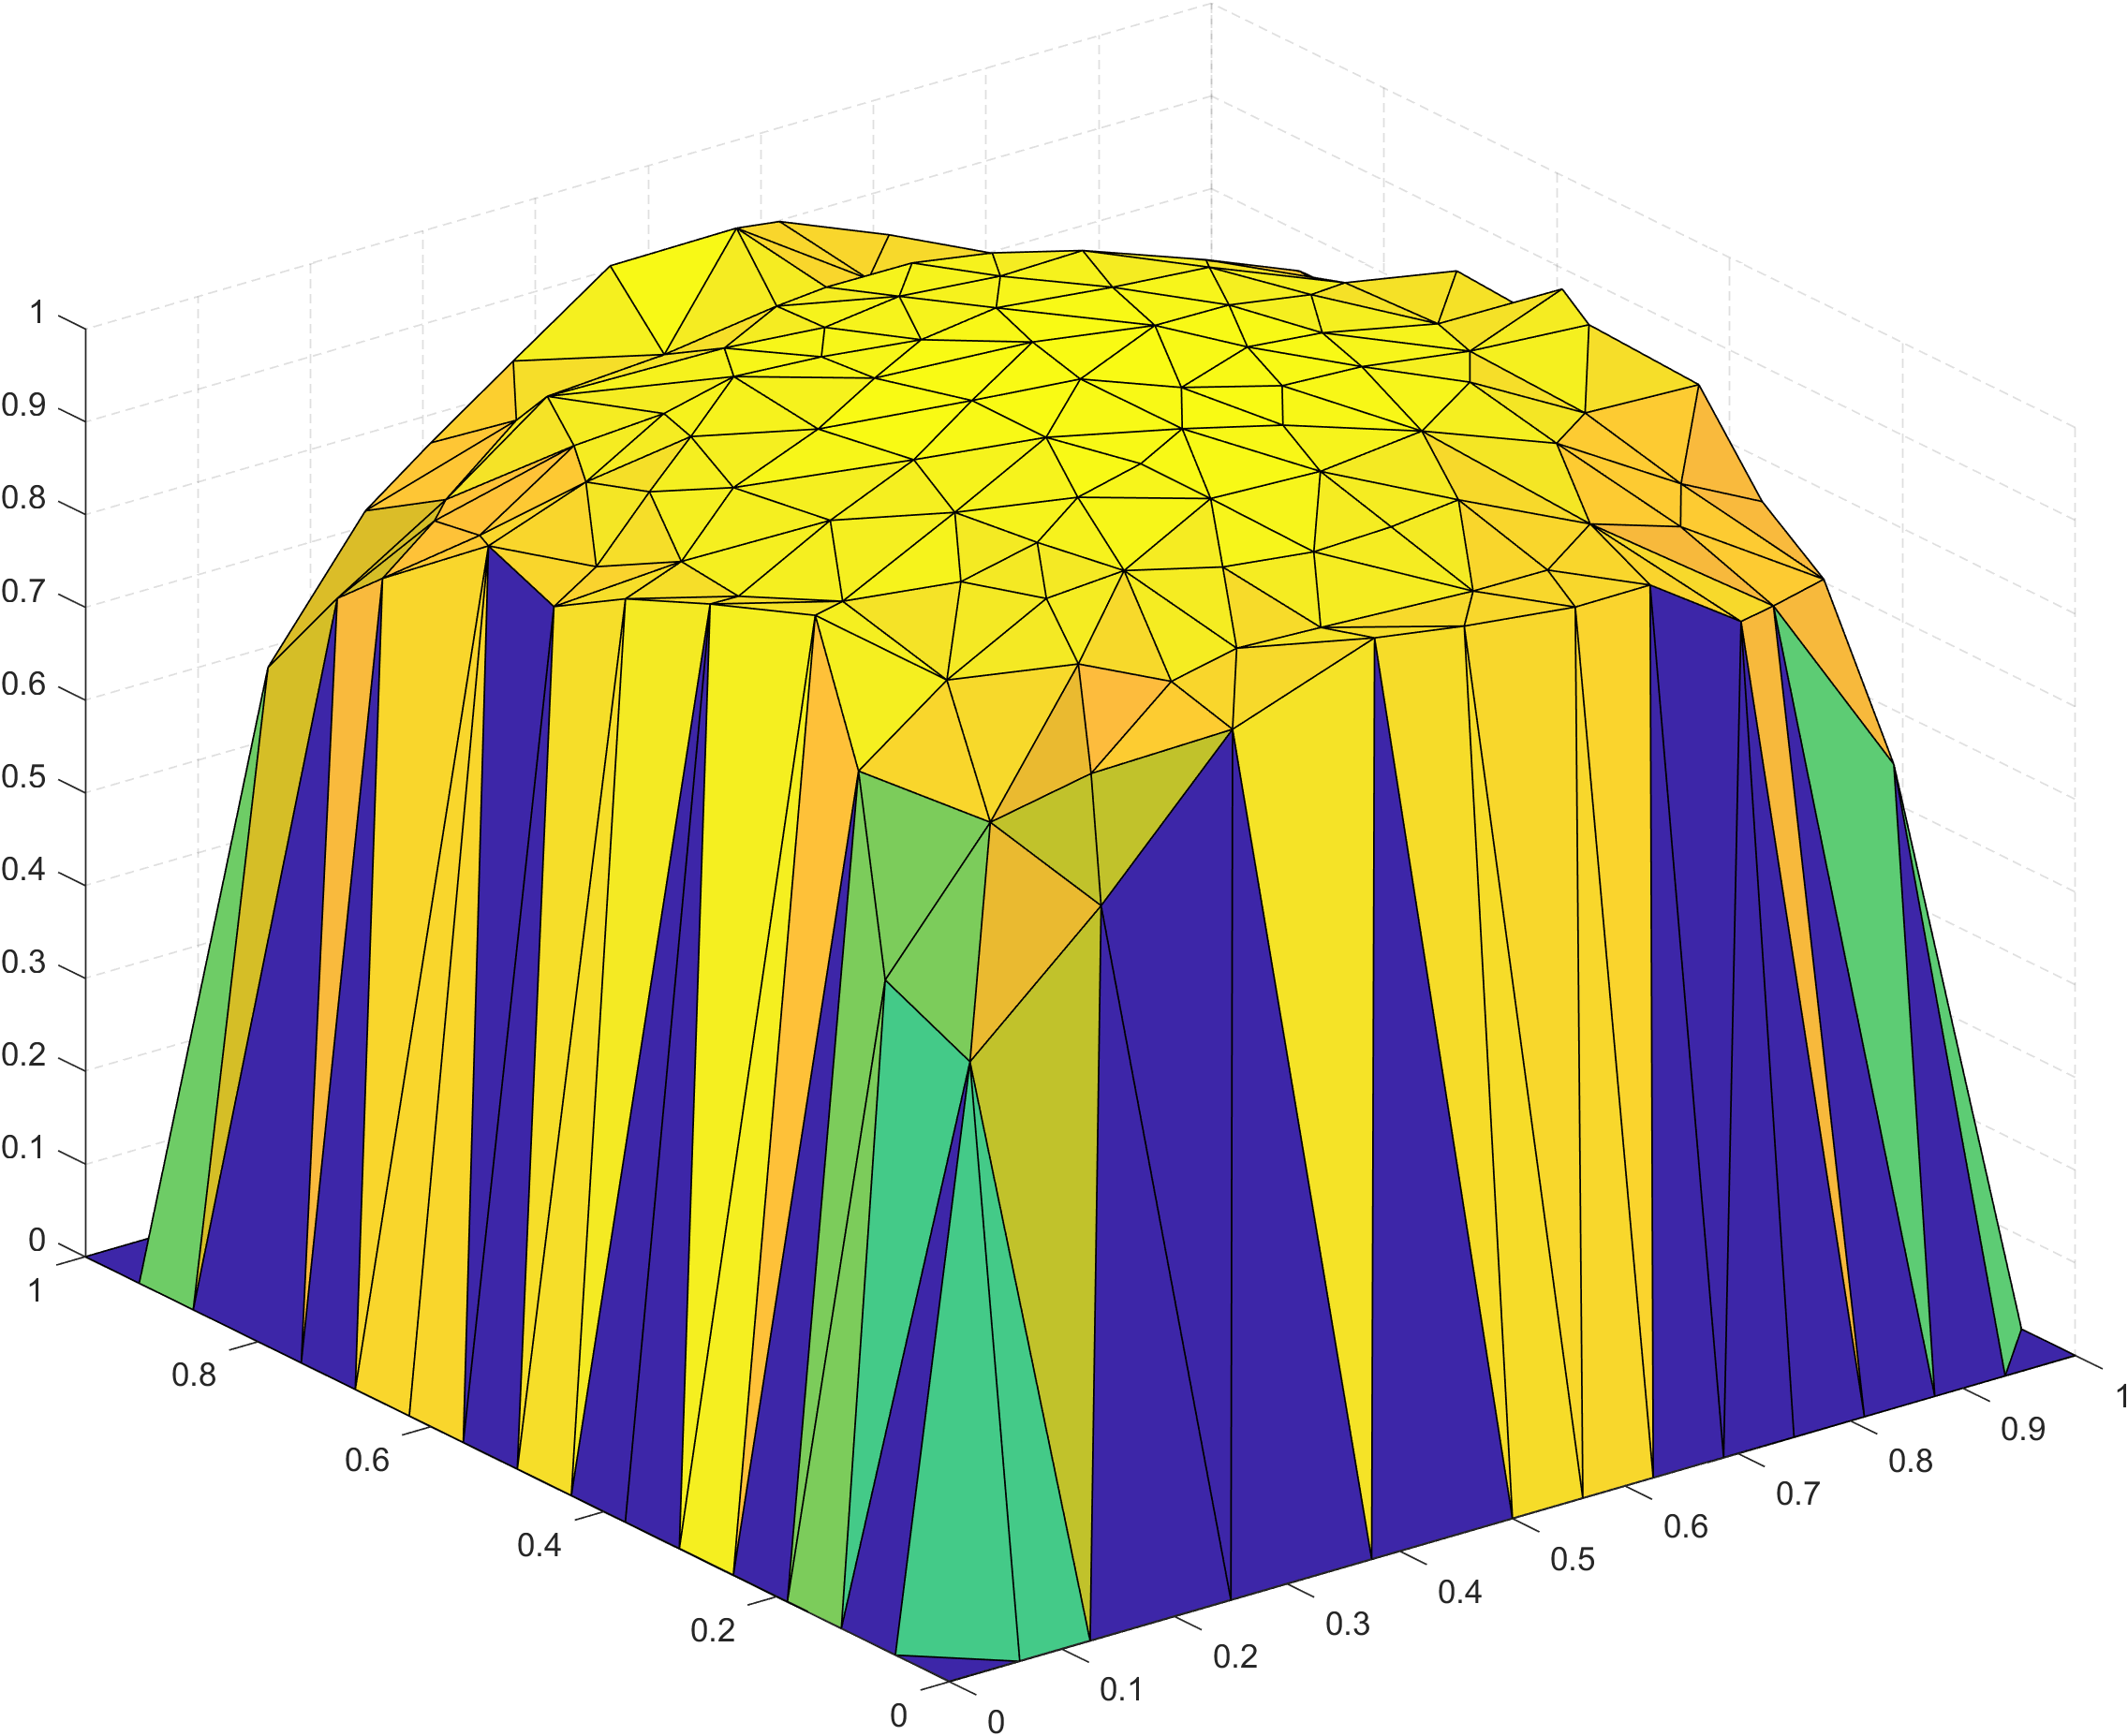
\includegraphics[height=\dimIm]{../Immagini/SDR2_CA_P1_AMax=0.005.png}
                            \caption{Soluzione qualitativa con \textit{ML}.}
                            \label{figSDR2TriangolazioniP1CA}
                        \end{subfigure}
                    }
                    \distR
        
                    \renewcommand{\lungSF}{.5\linewidth}
                    \renewcommand{\dimIm}{\linewidth}
                    \newcommand{\distC}{\hspace{7.5pt}} % Distanza tra le colonne
                    \makebox[\linewidth][c]{
                        \begin{subfigure}[t]{\lungSF}
                            \centering
                            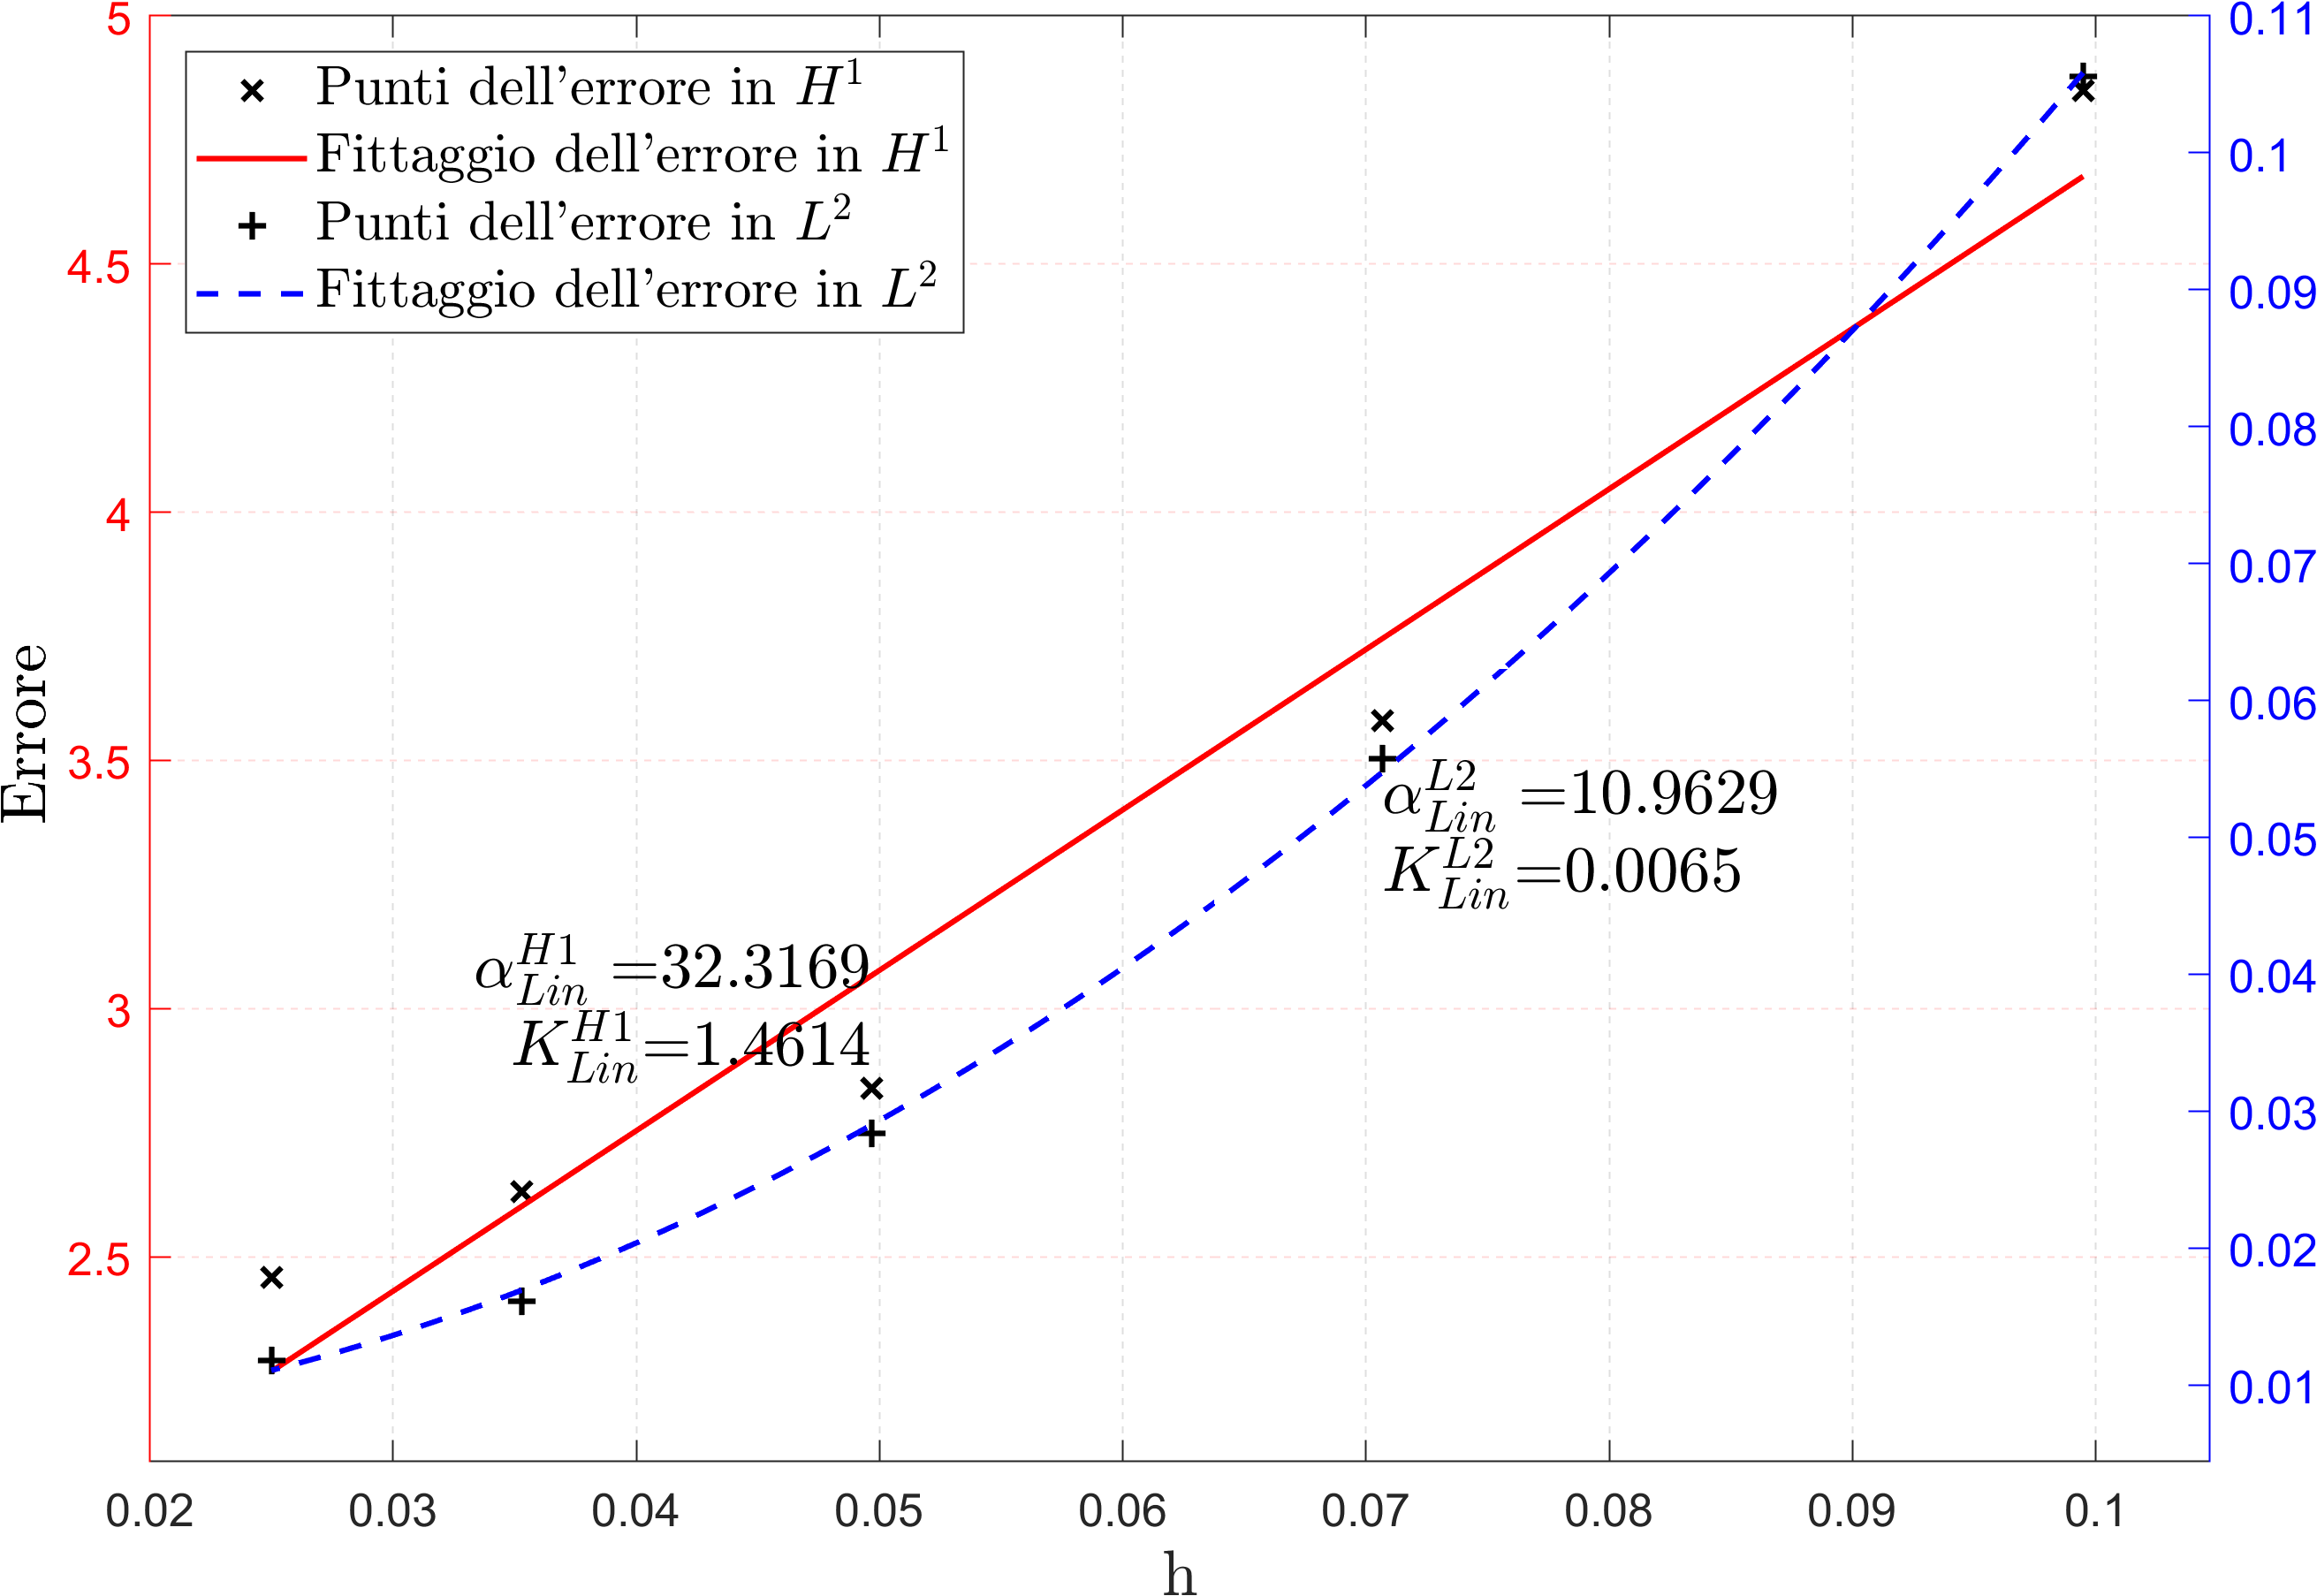
\includegraphics[width=\dimIm]{../Immagini/SDR2_P1_SA_ErrLin_AMax=0.01_NSim=5.png}
                        \caption{Errore in scala lineare senza \textit{ML}.}
                        \label{figSDR2ErroreP1LinSA}
                        \end{subfigure}
                        \distC
                        \begin{subfigure}[t]{\lungSF}
                            \centering
                            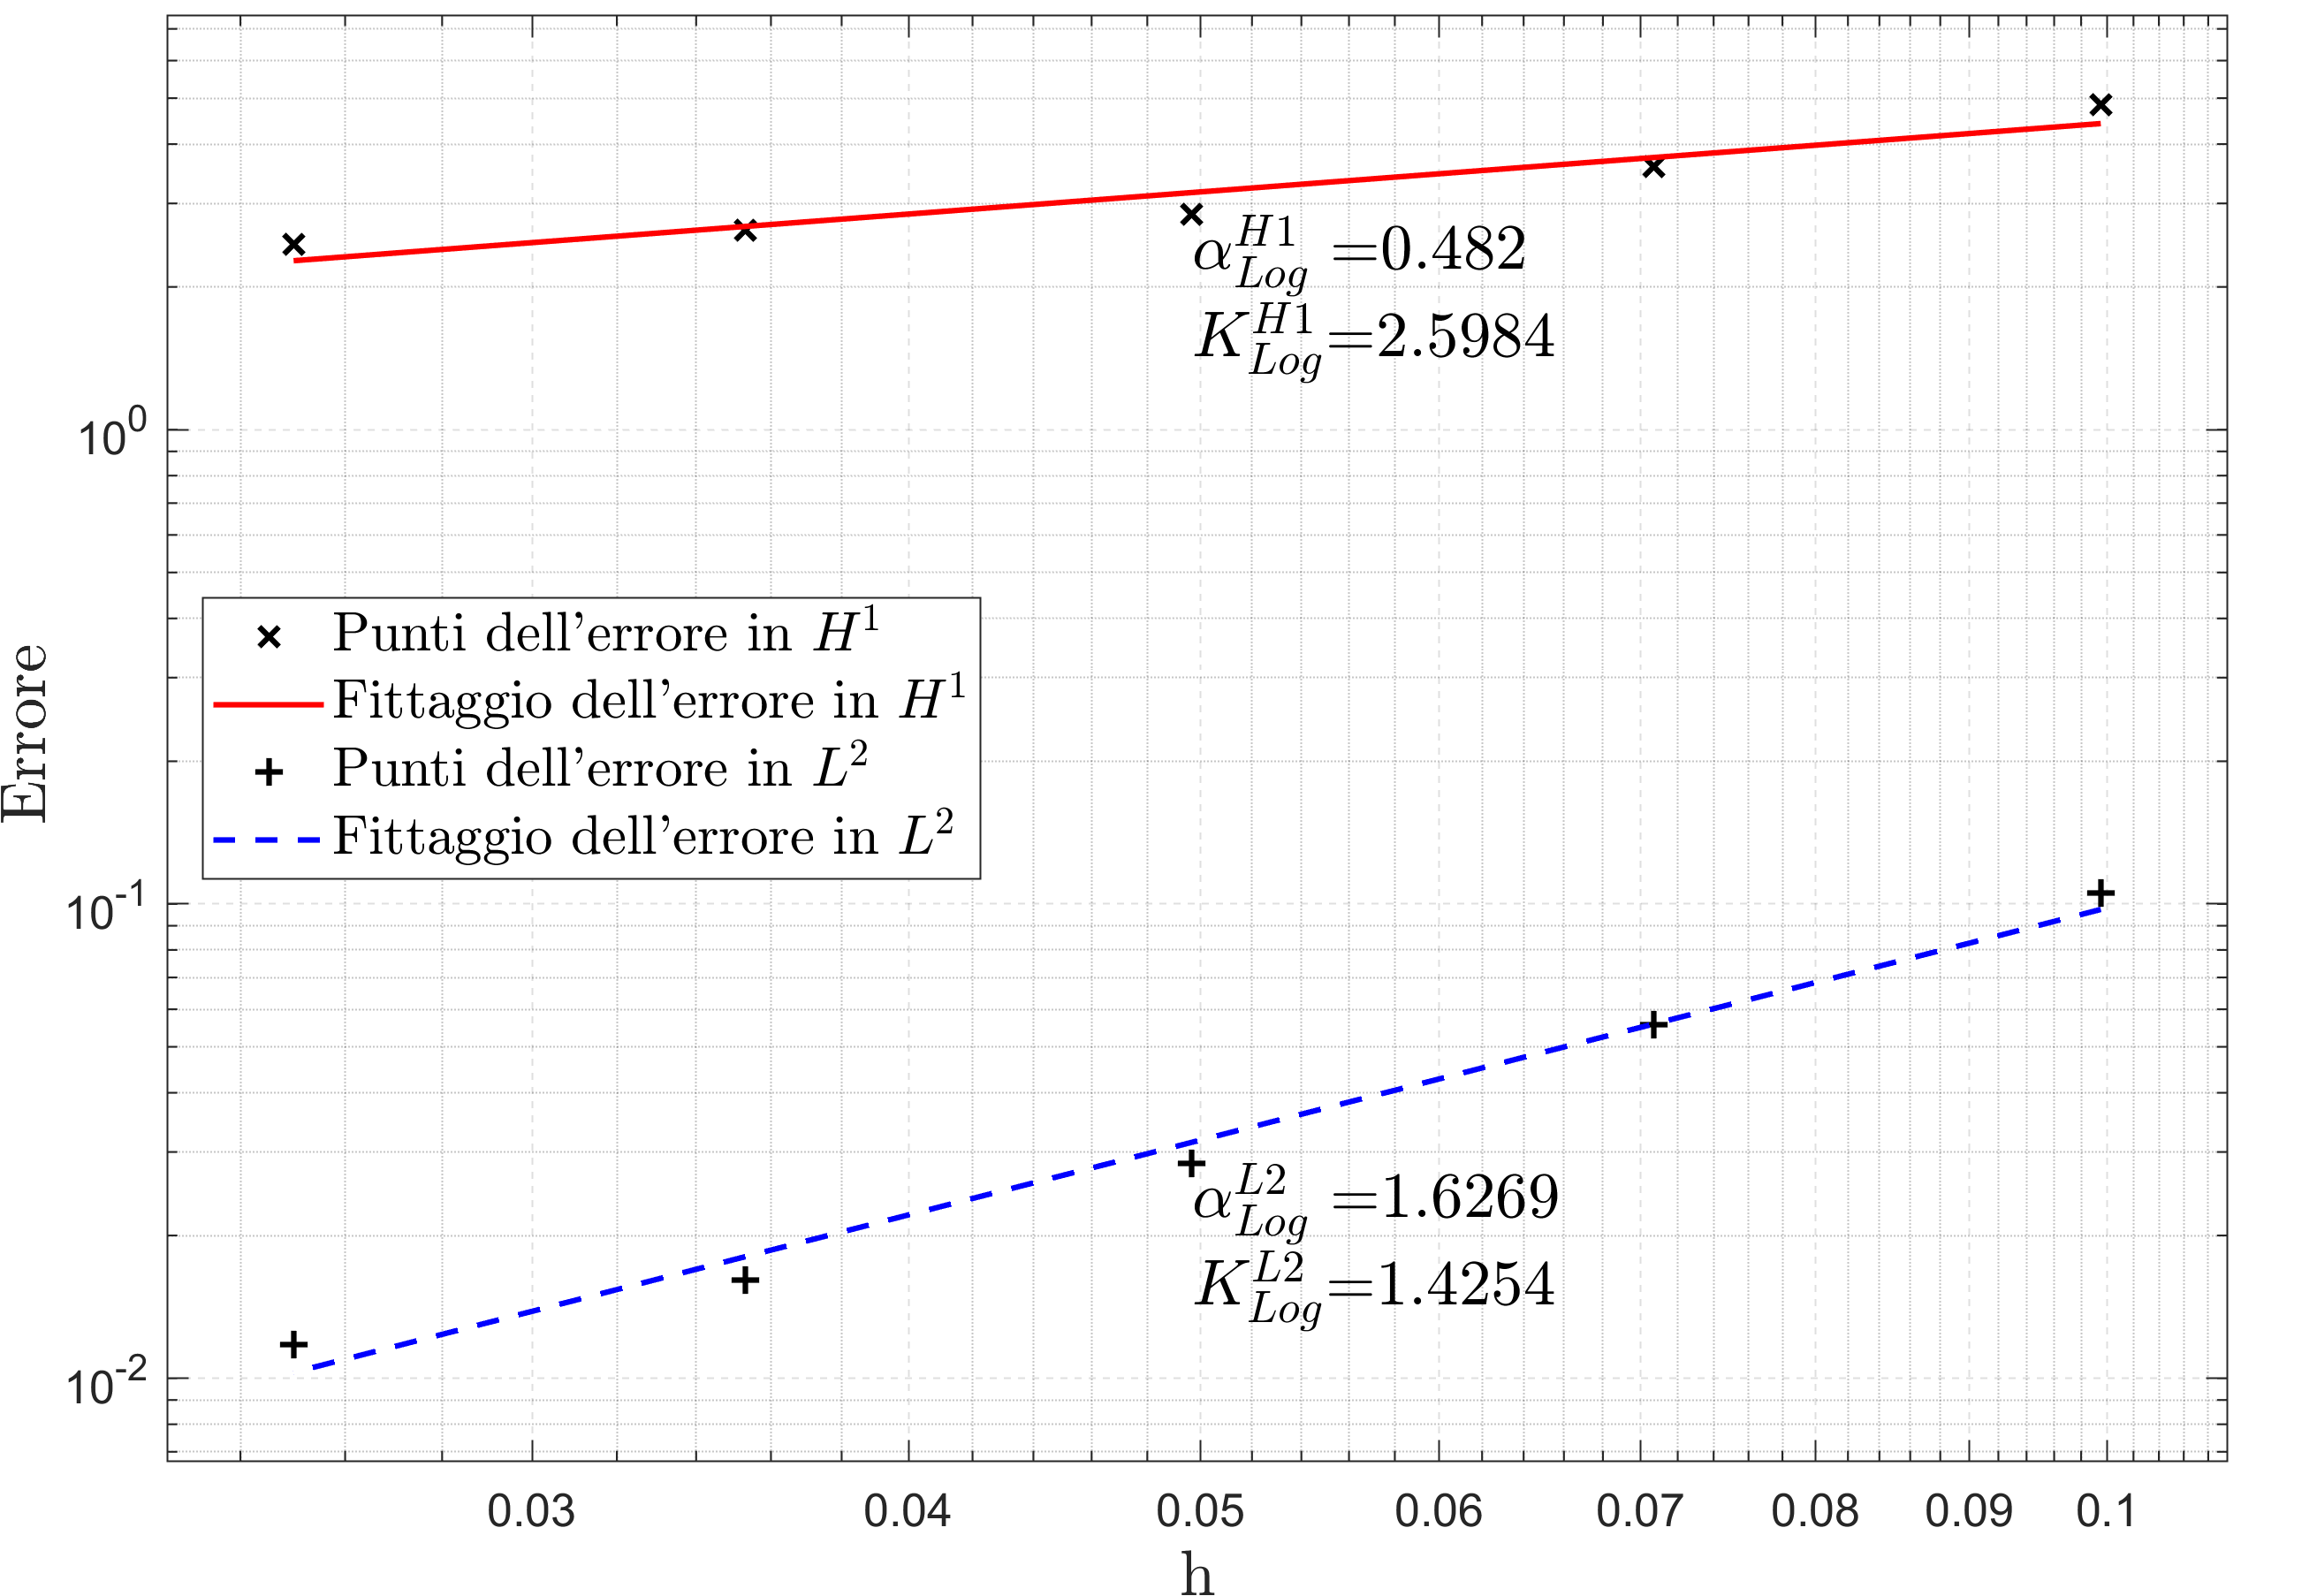
\includegraphics[width=\dimIm]{../Immagini/SDR2_P1_SA_ErrLog_AMax=0.01_NSim=5.png}
                        \caption{Errore in scala logaritmica senza \textit{ML}.}
                        \label{figSDR2ErroreP1LogSA}
                        \end{subfigure}
                    }
                    \distR
        
                    \makebox[\linewidth][c]{
                        \begin{subfigure}[t]{\lungSF}
                            \centering
                            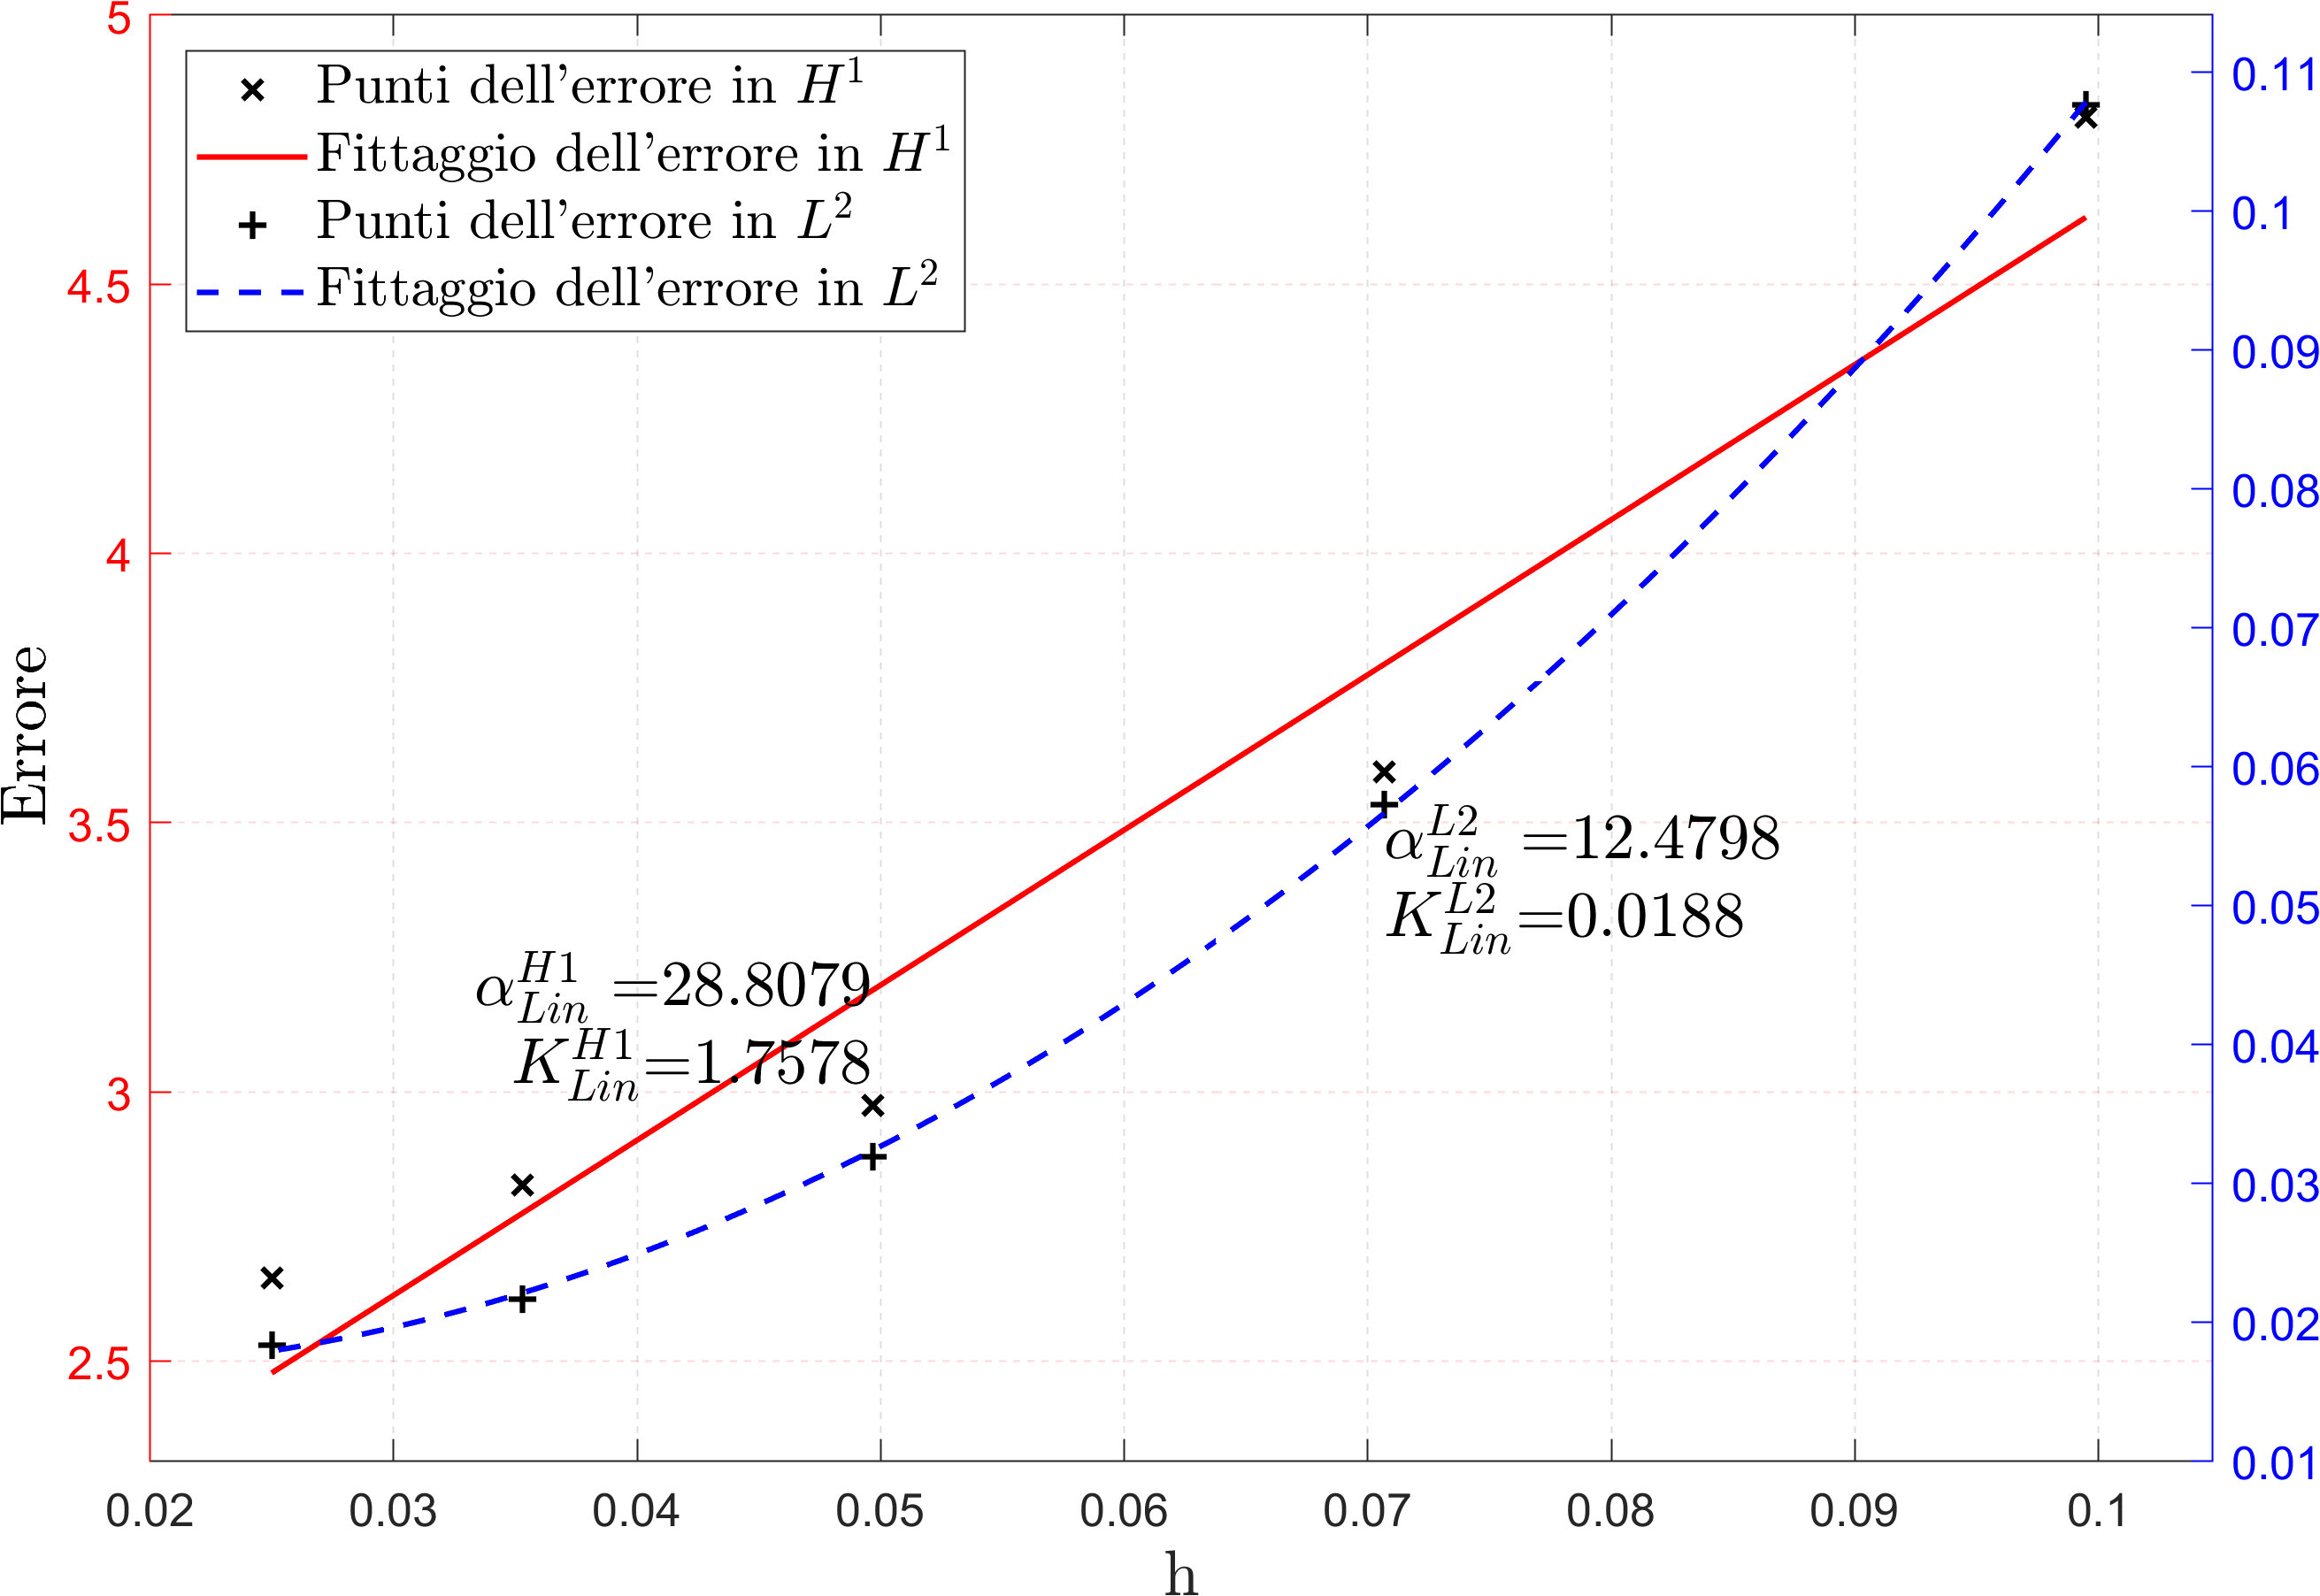
\includegraphics[width=\dimIm]{../Immagini/SDR2_P1_CA_ErrLin_AMax=0.01_NSim=5.png}
                        \caption{Errore in scala lineare con \textit{ML}.}
                        \label{figSDR2ErroreP1LinCA}
                        \end{subfigure}
                        \distC
                        \begin{subfigure}[t]{\lungSF}
                            \centering
                            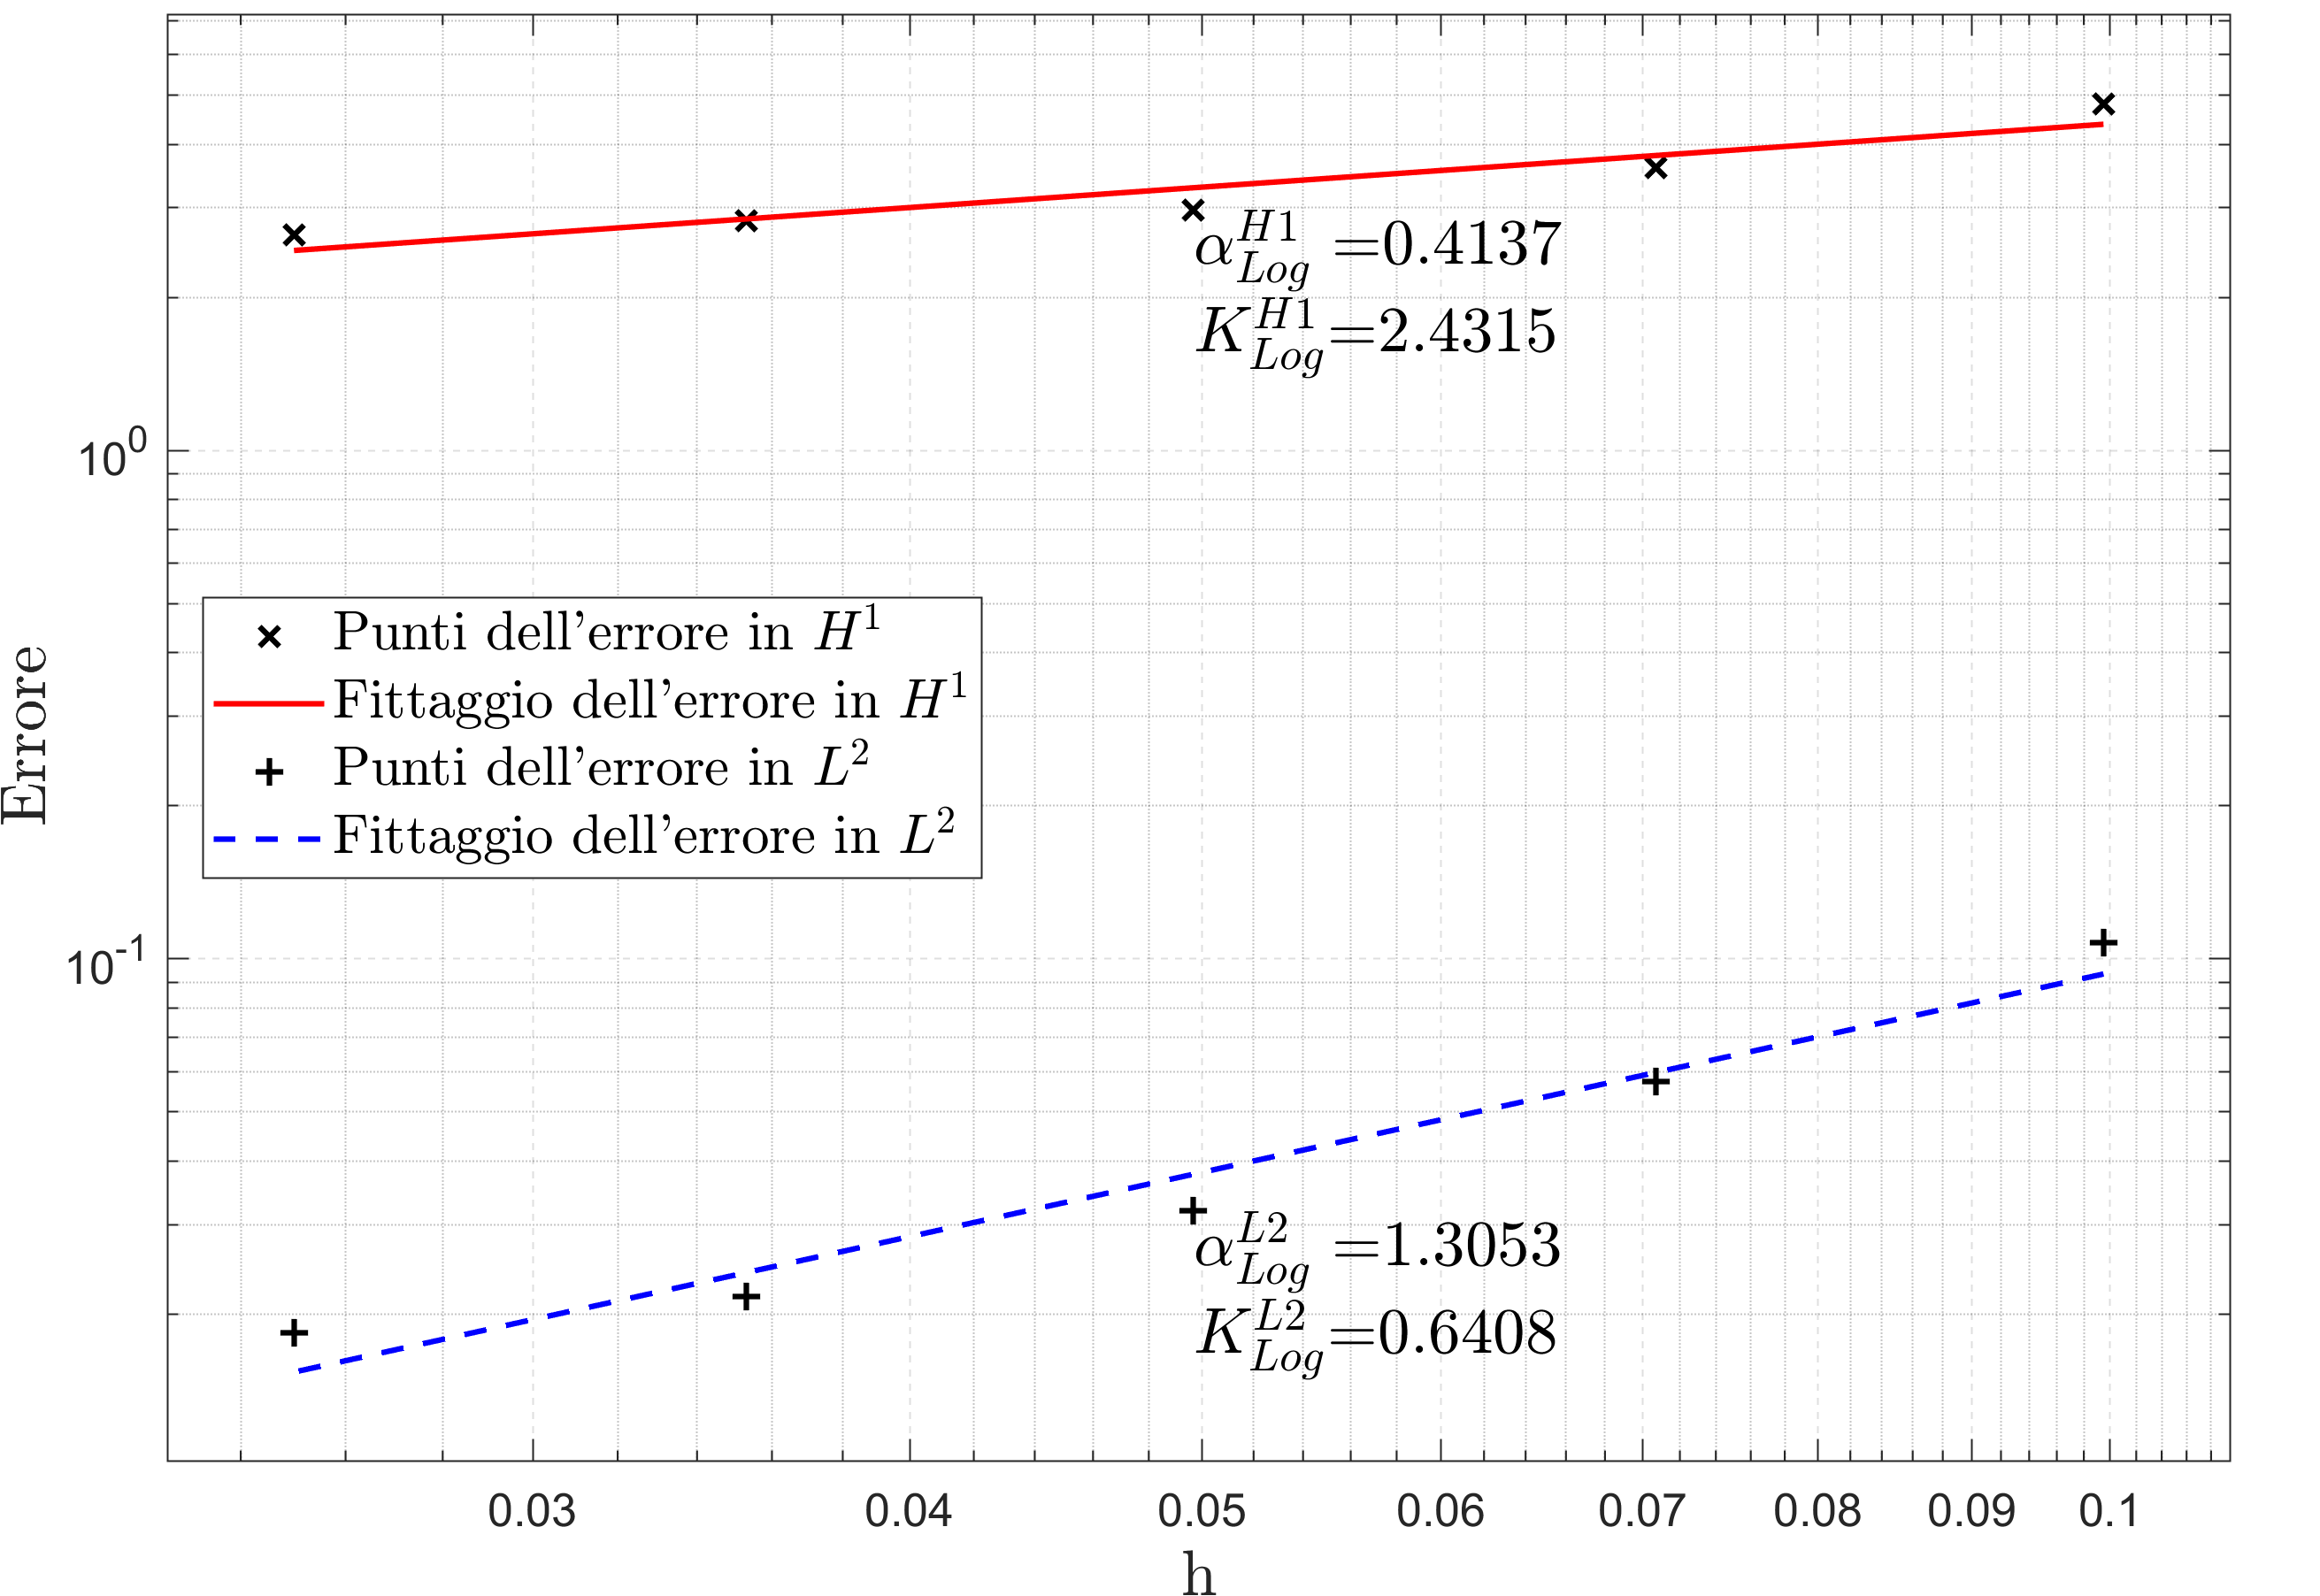
\includegraphics[width=\dimIm]{../Immagini/SDR2_P1_CA_ErrLog_AMax=0.01_NSim=5.png}
                        \caption{Errore in scala logaritmica con \textit{ML}.}
                        \label{figSDR2ErroreP1LogCA}
                        \end{subfigure}
                    }
                    \caption{Nelle Figg. \ref{figSDR2TriangolazioniEsatta}-\ref{figSDR2TriangolazioniP1CA} sono mostrate le soluzioni dell'SDR2: una esatta e le altre approssimate, coi $\mathbb{P}_1$, con e senza ammassamento; invece nelle \ref{figSDR2ErroreP1LinSA}-\ref{figSDR2ErroreP1LogCA} sono illustrati in due scale diverse gli errori in norma $H^1$ ed $L^2$, coi $\mathbb{P}_1$, con e senza ammassamento. I parametri dati a \textit{BBTR} sono spiegati nel $\S$\ref{parPremessaParametriBBTR}.}
                    \label{figSDR2}
                \end{figure*}
                %%%%%%%%%%%%%%%%%%
                %%%%%%%%%%%%%%%%%%
                %%%%%%%%%%%%%%%%%%

                %%%%%%%%%%%%%%%%%%%%%%%%%%%%
                %%% Tabella degli errori %%%
                %%%%%%%%%%%%%%%%%%%%%%%%%%%%
                {
                \setlength{\belowcaptionskip}{-0.3cm}
                \begin{table*}[t]
                    \centering
    
                        % Spaziatura globale
                    \newcommand{\lunST}{0.49\textwidth} % Lunghezza sottotabella
                    \newcommand{\sepTab}{\hspace{0.5cm}}  % Separazione delle tabelle
    
                        % Spaziatura locale
                    \newcommand{\sepCol}{\hspace{5pt}}
                    \newcommand{\lungTst}{0.5cm}
                    \renewcommand{\arraystretch}{1.5}
                    
                    \makebox[\textwidth][c]{
                    \begin{subtable}[t]{\lunST}
                        \centering
                        \begin{tabular}{c@{}|@{\sepCol}c@{\sepCol}c@{\sepCol}c@{\sepCol}c@{\sepCol}c@{\hspace{3pt}}c}
                            $h$&
                            \notaSci{9.95}{-2}&
                            \notaSci{7.07}{-2}&
                            \notaSci{4.97}{-2}&
                            \notaSci{3.53}{-2}&
                            \notaSci{2.50}{-2}\\
                            \hline
                            $\text{err}_{L^2}^{\mathbb P_1}$&
                                \notaSci{1.09}{-1}&
                                \notaSci{5.65}{-2}&
                                \notaSci{2.79}{-2}&
                                \notaSci{1.41}{-2}&
                                \notaSci{6.47}{-3}&
                                \multirow{2}{*}{\scriptsize\rotatebox{-90}{
                                \parbox{\lungTst}{SA}}}\\
                            $\text{err}_{H^1}^{\mathbb P_1}$&
                                \notaSci{3.84}{+0}&
                                \notaSci{2.84}{+0}&
                                \notaSci{2.14}{+0}&
                                \notaSci{1.61}{+0}&
                                \notaSci{1.10}{+0}\\
                            \hline
                            $\text{err}_{L^2}^{\mathbb P_1}$&
                                \notaSci{1.10}{-1}&
                                \notaSci{5.75}{-2}&
                                \notaSci{3.18}{-2}&
                                \notaSci{2.04}{-2}&
                                \notaSci{1.44}{-2}&
                                \multirow{2}{*}{\scriptsize\rotatebox{-90}{
                                \parbox{\lungTst}{CA}}}\\
                            $\text{err}_{H^1}^{\mathbb P_1}$&
                                \notaSci{3.77}{+0}&
                                \notaSci{2.91}{+0}&
                                \notaSci{2.44}{+0}&
                                \notaSci{2.07}{+0}&
                                \notaSci{1.74}{+0}
                        \end{tabular}
                        \caption{SDR1.}
                        \label{tabErroriSDR1}
                    \end{subtable}
                    \sepTab
                    \begin{subtable}[t]{\lunST}
                        \centering
                        \begin{tabular}{c@{}|@{\sepCol}c@{\sepCol}c@{\sepCol}c@{\sepCol}c@{\sepCol}c@{\hspace{3pt}}c}
                            $h$&
                            \notaSci{9.95}{-2}&
                            \notaSci{7.07}{-2}&
                            \notaSci{4.97}{-2}&
                            \notaSci{3.53}{-2}&
                            \notaSci{2.50}{-2}\\
                            \hline
                            $\text{err}_{L^2}^{\mathbb P_1}$&
                                \notaSci{1.06}{-1}&
                                \notaSci{5.57}{-2}&
                                \notaSci{2.84}{-2}&
                                \notaSci{1.61}{-2}&
                                \notaSci{1.18}{-2}&
                                \multirow{2}{*}{\scriptsize\rotatebox{-90}{
                                \parbox{\lungTst}{SA}}}\\
                            $\text{err}_{H^1}^{\mathbb P_1}$&
                                \notaSci{4.85}{+0}&
                                \notaSci{3.58}{+0}&
                                \notaSci{2.84}{+0}&
                                \notaSci{2.63}{+0}&
                                \notaSci{2.46}{+0}\\
                            \hline
                            $\text{err}_{L^2}^{\mathbb P_1}$&
                                \notaSci{1.08}{-1}&
                                \notaSci{5.73}{-2}&
                                \notaSci{3.19}{-2}&
                                \notaSci{2.16}{-2}&
                                \notaSci{1.84}{-2}&
                                \multirow{2}{*}{\scriptsize\rotatebox{-90}{
                                \parbox{\lungTst}{CA}}}\\
                            $\text{err}_{H^1}^{\mathbb P_1}$&
                                \notaSci{4.81}{+0}&
                                \notaSci{3.59}{+0}&
                                \notaSci{2.97}{+0}&
                                \notaSci{2.83}{+0}&
                                \notaSci{2.65}{+0}
                        \end{tabular}
                        \caption{SDR2.}
                        \label{tabErroriSDR2}
                    \end{subtable}
                    }
                    \caption{Dati relativi all'errore nell'SDR.}
                    \label{tabErroriSDR}
                \end{table*}
                }
                %%%%%%%%%%%%%%%%%%%%%%%%%%%%
                %%%%%%%%%%%%%%%%%%%%%%%%%%%%
                %%%%%%%%%%%%%%%%%%%%%%%%%%%%            


                Nonostante la non evidente instabilità, si potrebb'essere tentati a stabilizzare il problema mediante il metodo d'ammassamento o di \textit{mass lumping} (\textit{MP}) in inglese. A tal fine si scomponga l'operatore $a$ nella \eqref{eqOperatoreBilinearePSVariazionale} come somma di tre operatori
                %
                \begin{equation*}
                    \setlength{\thinmuskip}{1mu}
                    \setlength{\medmuskip}{2mu}
                    \setlength{\thickmuskip}{3mu}
                    \begin{aligned}
                        d:\ &H^1(\Omega)\!\times\!H^1(\Omega)
                        \rightarrow\mathbb R\\
                        &(u,v)\mapsto d(u,v)\equiv
                        \int_{\Omega}\nu\nabla u\cdot\nabla v\,\de x,\\
                        c:\ &H^1(\Omega)\!\times\!H^1(\Omega)
                        \rightarrow\mathbb R\\
                        &(u,v)\mapsto c(u,v)\equiv
                        \int_{\Omega}\boldsymbol\beta\cdot\nabla uv\,\de x,\\
                        r:\ &H^1(\Omega)\!\times\!H^1(\Omega)
                        \rightarrow\mathbb R\\
                        &(u,v)\mapsto r(u,v)\equiv
                        \int_{\Omega}\sigma uv \,\de x,
                    \end{aligned}
                    \label{eqOperatoriBilineariPVAmmassamento}
                \end{equation*}
                %
                che matricialamente corrisponde alla scomposizione della matrice di rigidezza $\mathbf A$ nelle somma
                %
                \begin{equation}
                    \mathbf A=\mathbf D+\mathbf C+\mathbf R,
                    \label{eqScomposizioneMatriceRigidezza}
                \end{equation}
                %
                ove
                %
                \begin{equation*}
                    \begin{aligned}
                        \mathbf D&\in\mathbb R^{\Ngdl\times\Ngdl}
                        &&\text{con}\;(\mathbf D)_{i,j}=d(\varphi_j,\varphi_i),\\
                        \mathbf C&\in\mathbb R^{\Ngdl\times\Ngdl}
                        &&\text{con}\;(\mathbf C)_{i,j}=c(\varphi_j,\varphi_i),\\
                        \mathbf R&\in\mathbb R^{\Ngdl\times\Ngdl}
                        &&\text{con}\;(\mathbf R)_{i,j}=r(\varphi_j,\varphi_i),\\
                    \end{aligned}
                    \label{eqScomposizioneADefinizioneMatrici}
                \end{equation*}
                %
                sono ordinatamente la matrice di diffusione, di convezione e di reazione. Ecco l'ammassamento consiste nella definizione della matrice diagonale $\mathbf S$ tale che
                %
                \begin{equation*}
                    (\mathbf S)_{i,j}=\delta_{ij}\sum_{k=1}^{\Ngdl}(\mathbf R)_{i,k},
                    \label{eqTrasformazioneMatriceR}
                \end{equation*}
                %
                col $\delta_{ij}$ uguale alla delta di Kronecker, la quale va sostituita alla $\mathbf R$ nella \eqref{eqScomposizioneMatriceRigidezza} cosí da definire una matrice di rigidezza stabilizzata
                %
                \begin{equation*}
                    \mathbf A_\text{s}\equiv\mathbf D+\mathbf C+\mathbf S,
                    \label{eqScomposizioneMatriceRigidezzaAmmassata}
                \end{equation*}
                %
                colla quale si può risolvere il sistema definito dalla \eqref{eqSistemaAlgebrico}.

                Cosí procedendo le soluzioni ammassate sono illustrate nelle Figg. \ref{figSDR1TriangolazioniP1CA} e \ref{figSDR2TriangolazioniP1CA}, e paiono, almeno qualitativamente, ridurre lievemente le oscillazioni. Cionnonostante, da un punto di vista quantitativo gli errori presentano ordini di convergenza minori oltre che errori maggiori, com'è evidente dalle Figg. \ref{figSDR1ErroreP1LinSA} e \ref{figSDR1ErroreP1LogSA} per l'SDR1 e nelle Figg. \ref{figSDR2ErroreP1LinSA} e \ref{figSDR2ErroreP1LogSA} per l'SDR2 (i relativi dati si trovano rispettivamente nelle Tabb. \ref{tabErroriSDR1} e \ref{tabErroriSDR2}, e sono contrassegnati dalle righe coll'acronimo CA nell'ultima colonna).

                Questo peggioramento potrebbe discendere, nonostante le forti ripidità nelle soluzioni, dalle insufficienti instabilità presenti nelle soluzioni \eqref{eqSoluzioneEsattaSDR1} e \eqref{eqSoluzioneEsattaSDC2}, tali da giustificare una correzione mediante ammassamento: è un po' come aggiungere una toppa a un vestito nuovo, anziché usarla per ripararne uno vecchio.

                Si nota infine che l'ammassamento rompe i $\mathbb P_2$ come mostrato nella Fig. \ref{figSDRP2CA}, e questa è la ragione per cui sono stati tralasciati in questo paragrafo.

                \begin{figure}[H]
                    \centering 
                    \newcommand{\lungSF}{.5\linewidth}
                    \newcommand{\dimIm}{\linewidth}
                    \makebox[\linewidth][c]{
                        \begin{subfigure}[t]{\lungSF}
                            \centering
                            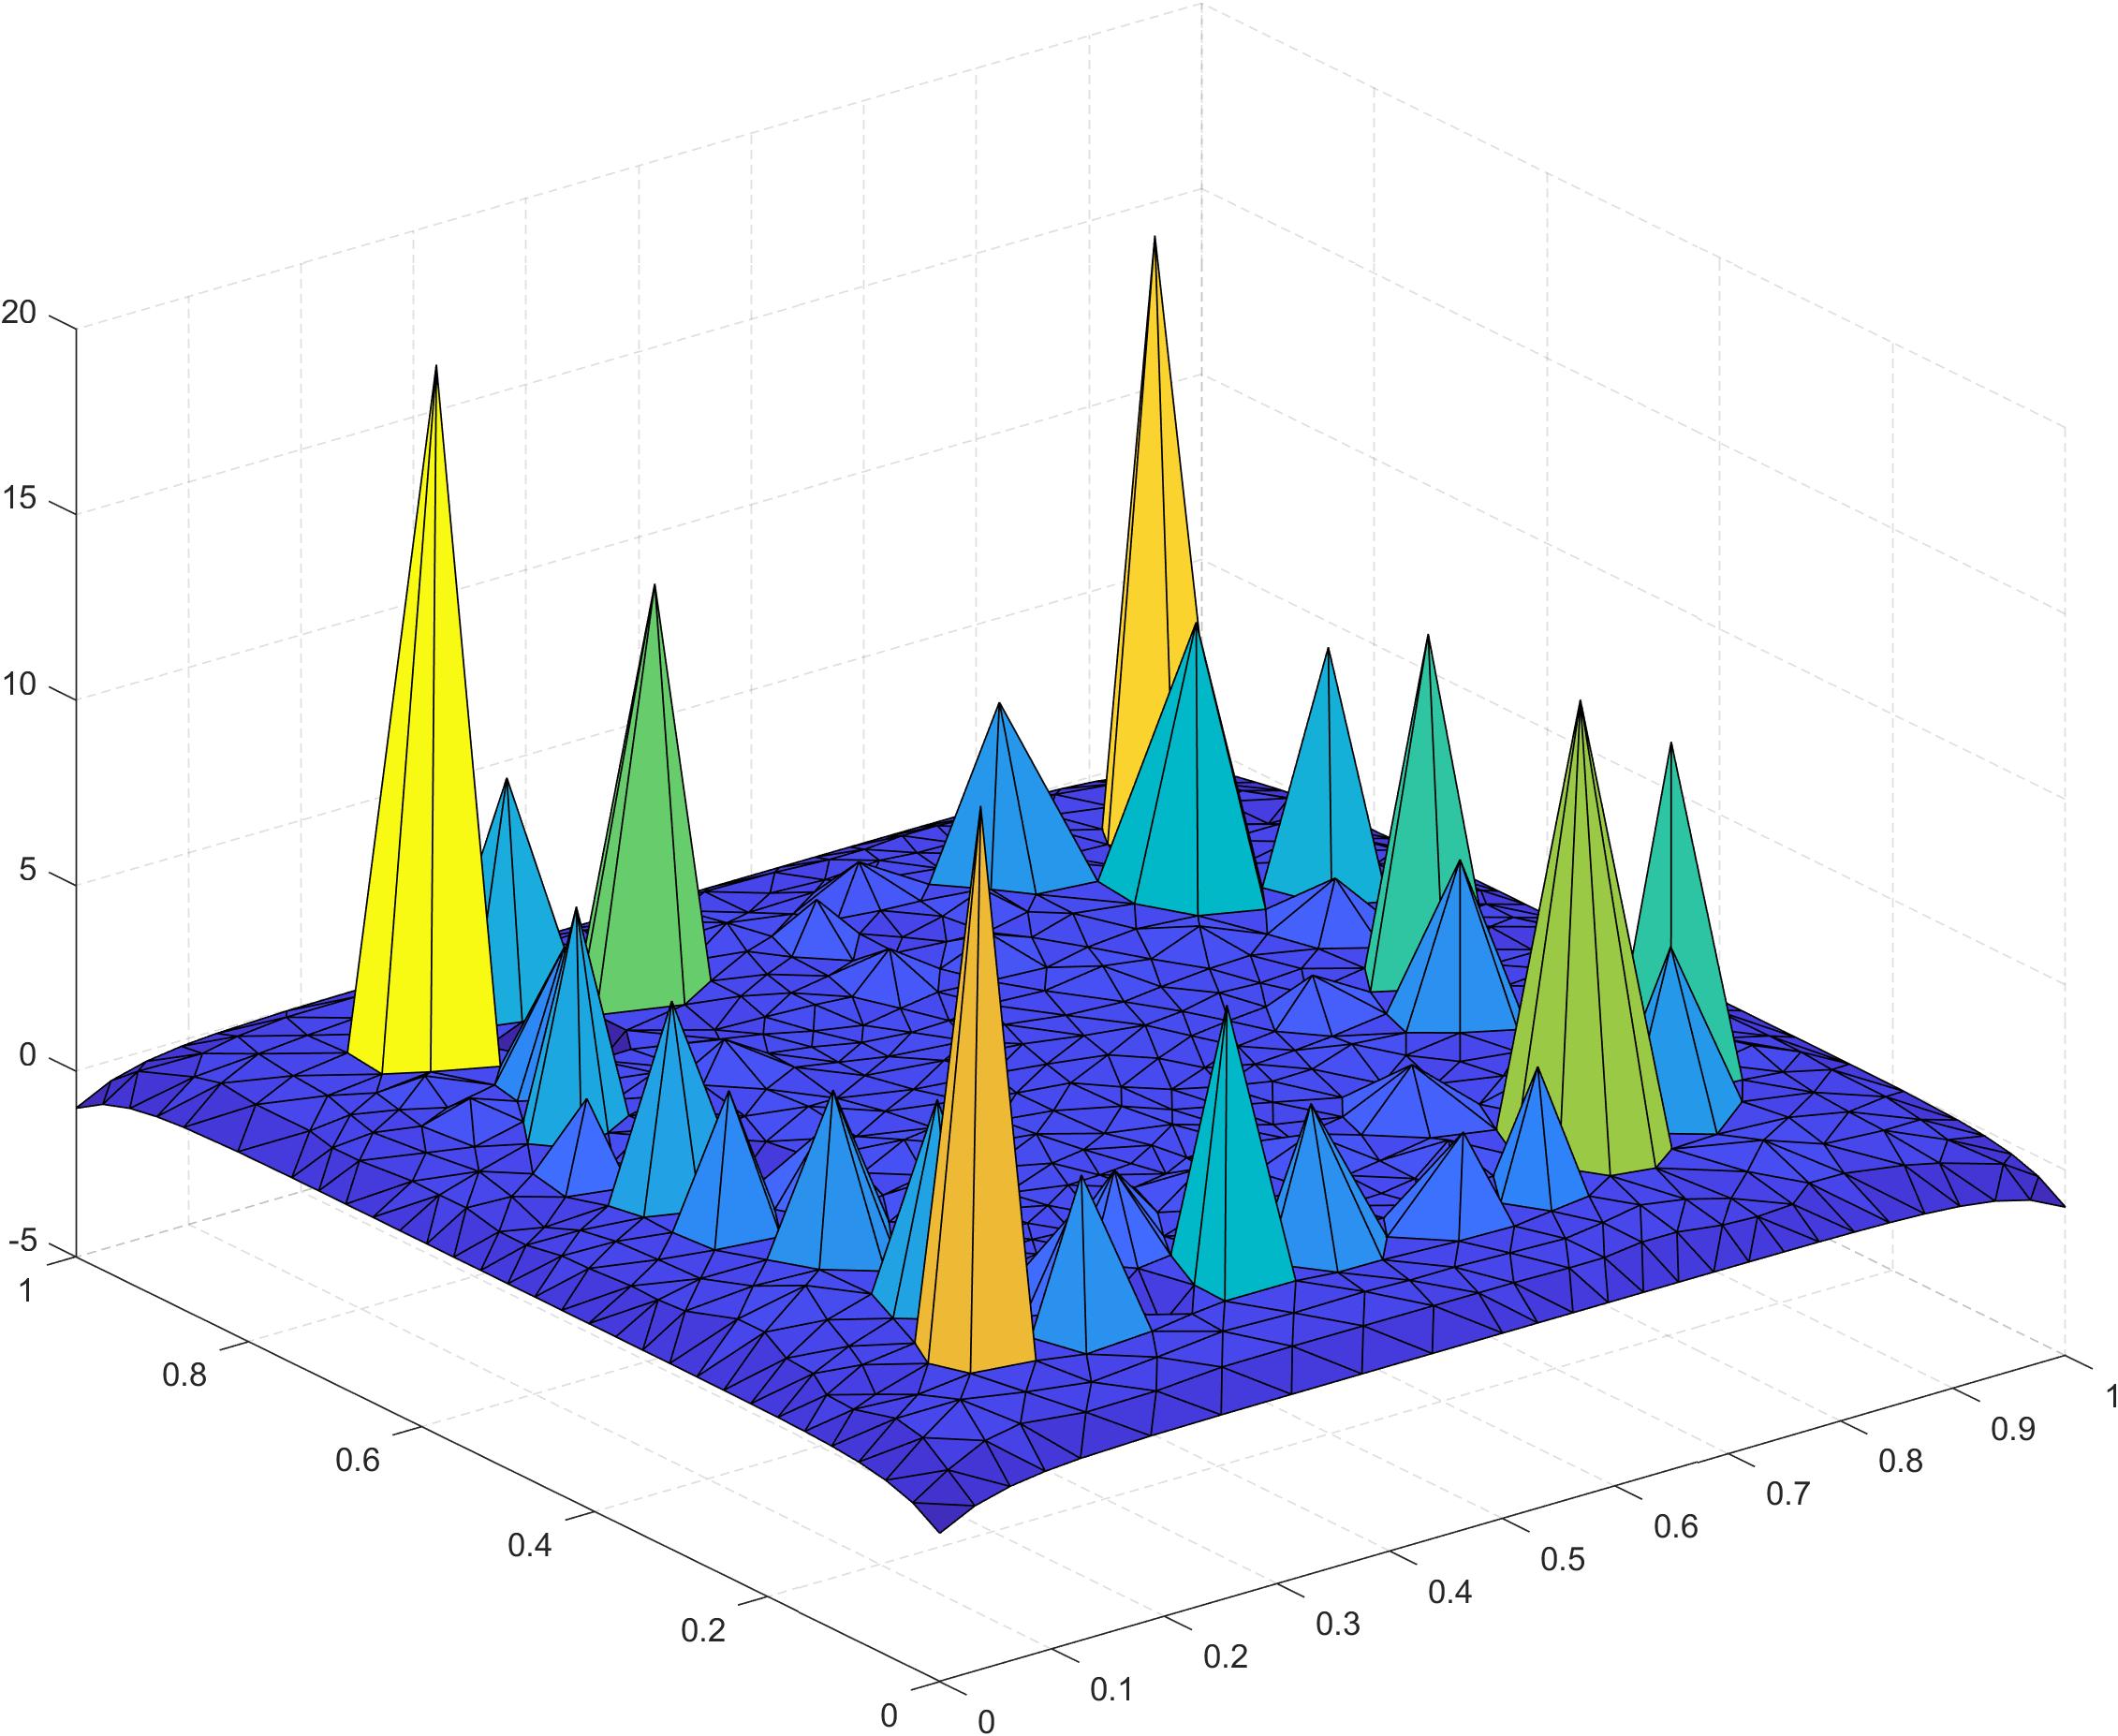
\includegraphics[width=\dimIm]{../Immagini/SDR1_CA_P2_AMax=0.005.png}
                            \caption{SDR1.}
                            \label{figSDR1P2CA}
                        \end{subfigure}
                        \begin{subfigure}[t]{\lungSF}
                            \centering
                            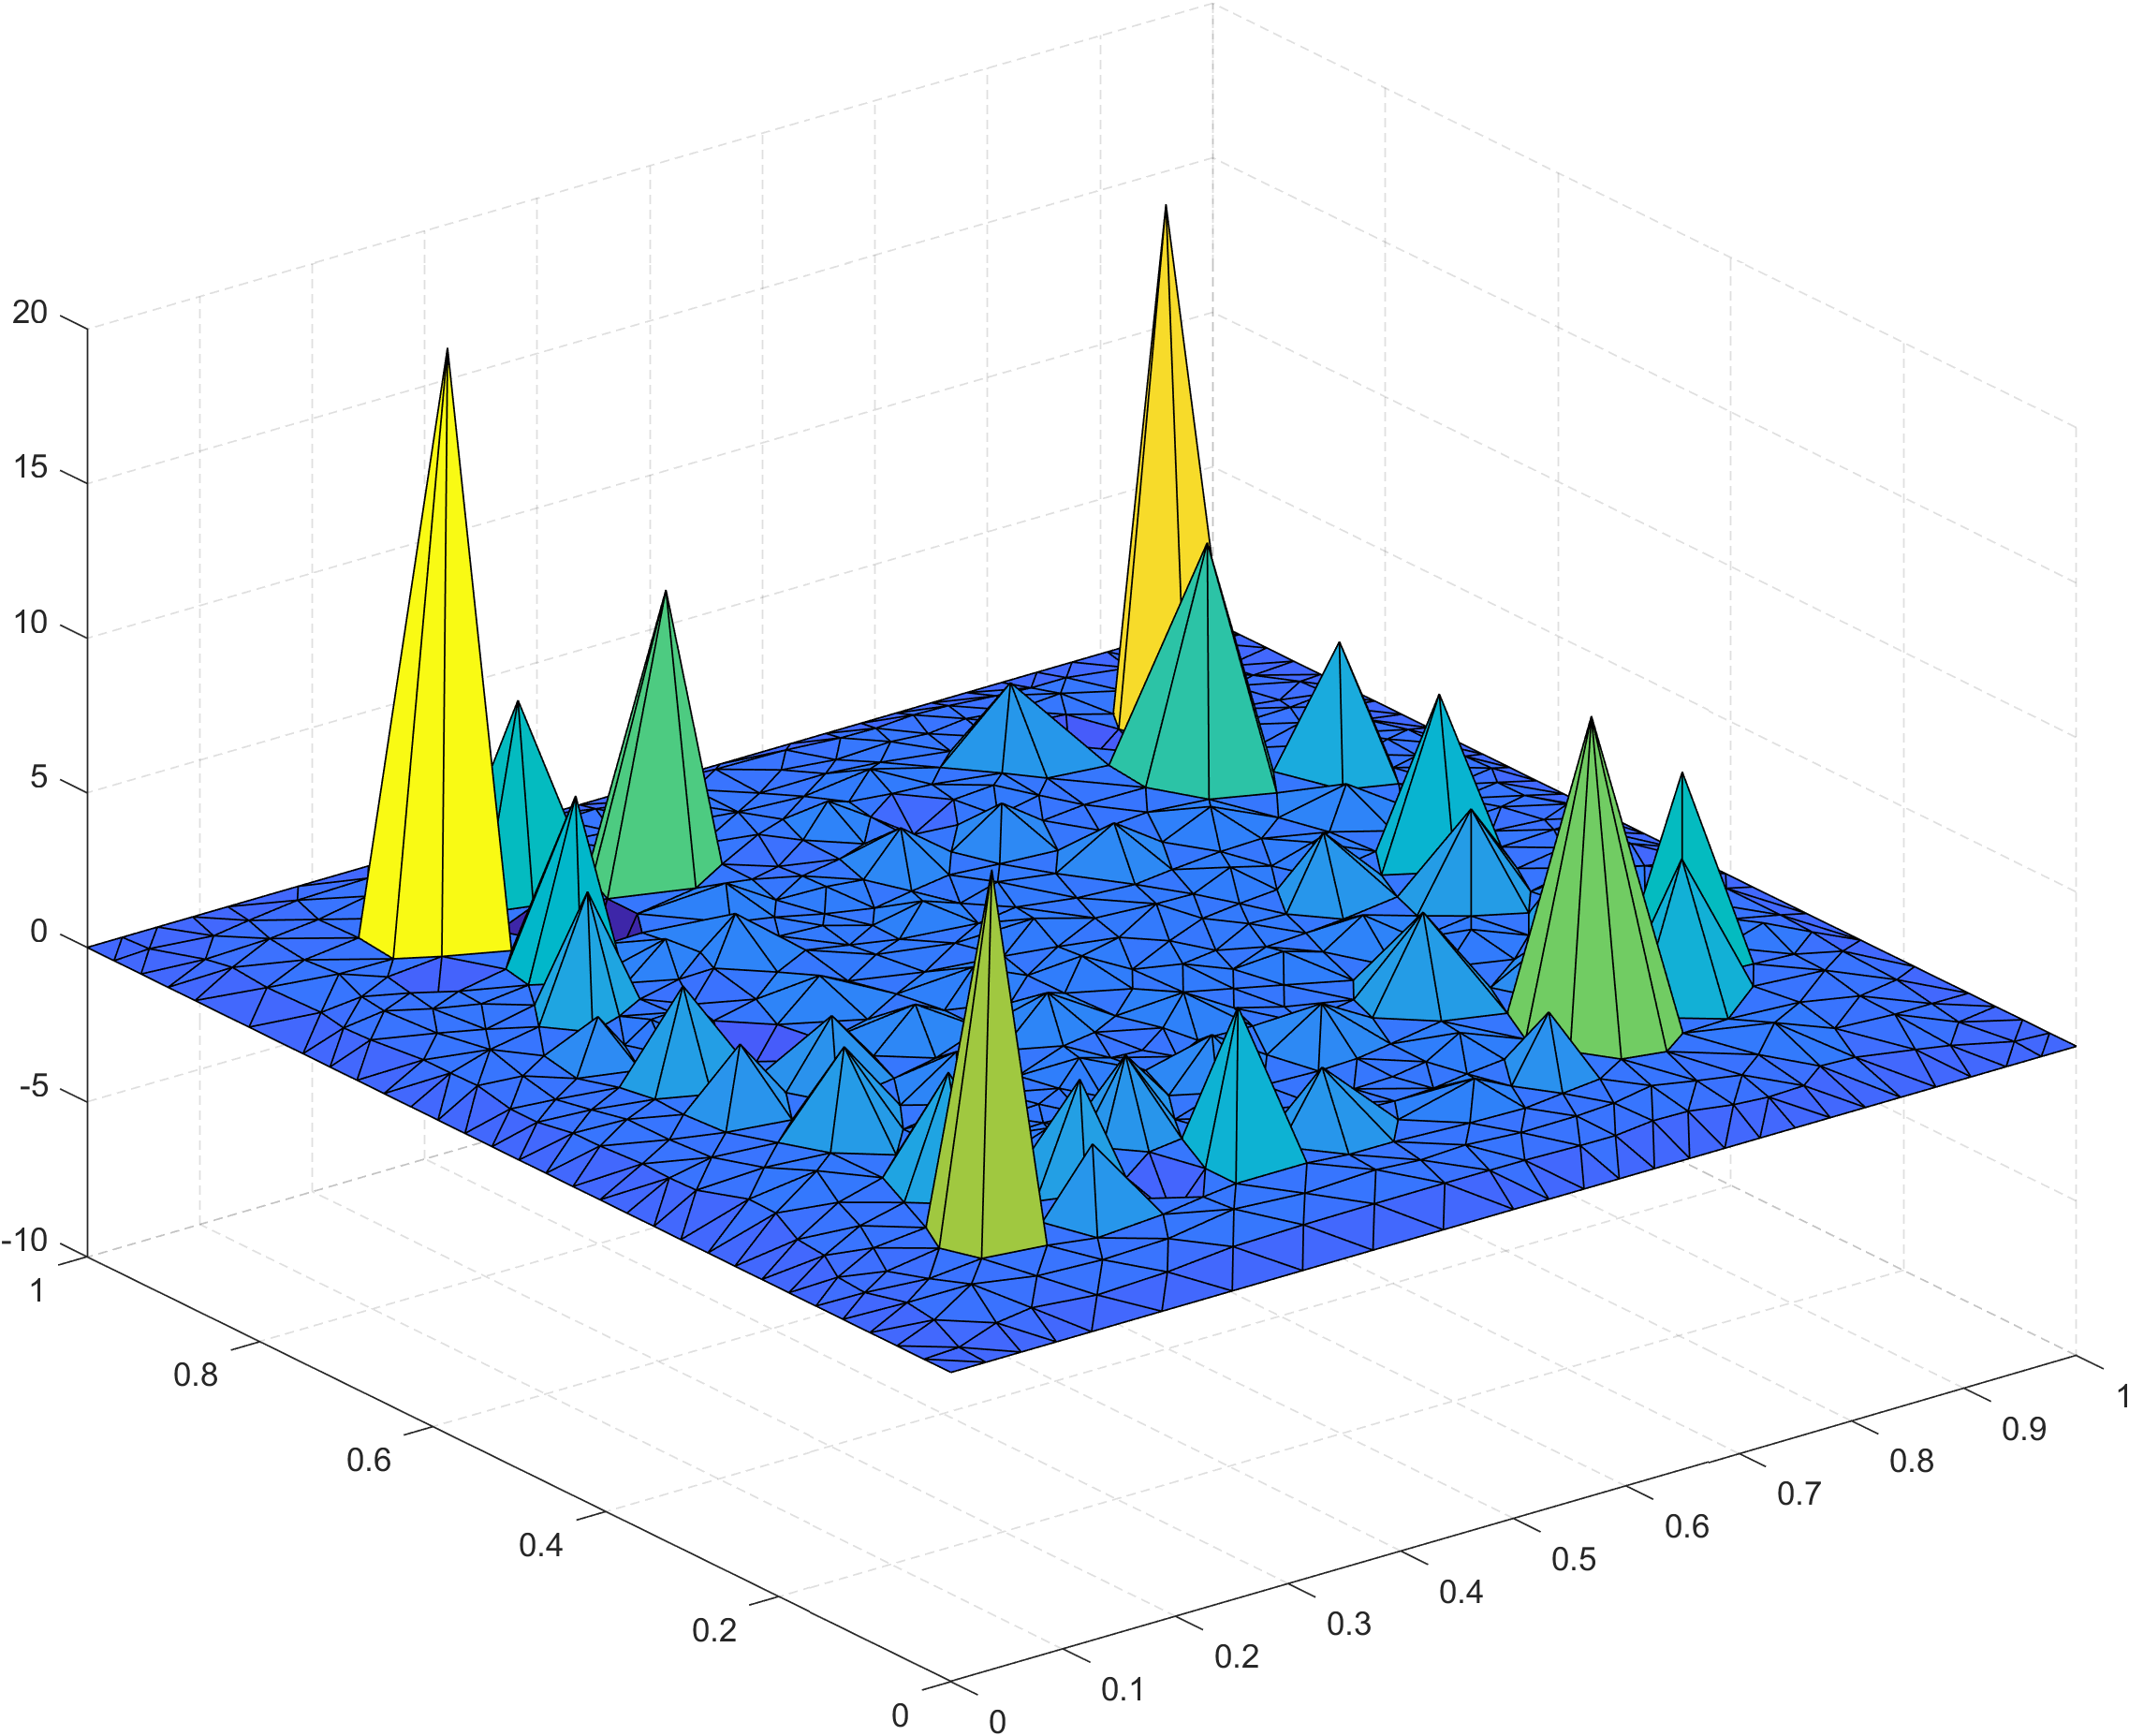
\includegraphics[width=\dimIm]{../Immagini/SDR2_CA_P2_AMax=0.005.png}
                            \caption{SDR2.}
                            \label{figSDR2P2CA}
                        \end{subfigure}
                    }
                    \caption{Soluzioni qualitative dell'SDR coi $\mathbb P_2$ ed \textit{ML}.}
                    \label{figSDRP2CA}
                \end{figure}

            
        \subsection{Problemi Evolutivi (E)}
        \setcounter{subsubsection}{-1}

            Prima di sviscerare i vari casi di studio evolutivi è necessaria una premessa sulle funzioni da usare per gli errori.

            \subsubsection{Errori in spazio e in tempo}\label{parProblemaEvolutivoErrori}

                Si è ora interessati a verificare gli ordini di convergenza sia dello schema di Crank–Nicolson (CN) che dei soliti $\mathbb P_1$ e $\mathbb P_2$ in un contesto evolutivo descritto nel $\S$\ref{ParProblemaEvolutivo}.
    
                {\SpaziaturaMate{1}{2}{3}
                In questo si ha che $f:\Omega\times[0,T]\to\mathbb R$ può dipendere sia dallo spazio che dal tempo, e dunque potenzialmente si commetterà un errore sia in spazio che in tempo.
                
                Pertanto, per agevolare lo studio, si può scomporre la $f$ come somma di due funzioni $g:\Omega\to\mathbb R$ ed $h:[0,T]\to\mathbb R$, ovvero}
                %
                \begin{equation*}
                    f(x,y,t)\equiv g(x,y)+h(t),
                \end{equation*}
                %
                che equivale a rendere indipendenti gli errori: quello in spazio è attribuibile solo a $g$, mentre quello in tempo esclusivamente ad $h$.
                
                Dopodiché si può fare in modo, a seconda del caso di studio considerato, che una funzione appartenga allo spazio generabile dal metodo considerato e l'altra no; ad es. se si vuole apprezzare l'ordine di convergenza di CN si può porre
                %
                \begin{equation*}
                    g(x,y)\in\mathbb P_k\quad
                    \text{e}\quad
                    h(t)\notin V(\text{CN}),
                \end{equation*}
                %
                ove $k=1,2$ e con $V(\text{CN})$ si è indicato lo spazio approssimabile esattamente dallo schema di Crank-Nicolson; cosí procedendo la parte in spazio compierà un errore trascurabile [dell'ordine della precisione di macchina], mentre la parte in tempo ne compierà uno che decaderà secondo CN.
    
                In totale i casi di studio sono cinque: i primi due fissano lo spazio e scandiscono il tempo, mentre i successivi due fissano il tempo e scandiscono lo spazio, secondo le regole già viste nel $\S$\ref{parPremessaParametriBBTR}; l'ultimo, invece, non considera gli errori ed è solo illustrato qualitativamente a conclusione di questa relazione.
                
                {\SpaziaturaMate{1}{2}{3}
                Inoltre in tutti si pone $T=1$, $\nu=1$, $\beta=(1,1)^\top$ e $\sigma=1$}, che equivale a trasformare il \teqref{eqProblemaEllitticoEvolutivo}{[PE]} in
                %
                \begin{equation}
                    \SpaziaturaMate{1}{2}{3}
                    \left\{
                    \begin{aligned}
                        \derP ut-\Delta u+\derP ux+\derP uy+u&=f&\text{in }&\Omega\times(0,1], \\
                                u&=u\vert_{\partial\Omega}&\text{su }&\partial\Omega\times(0,1],\\
                        u&=u\vert_{t=0} &\text{su }&\Omega,\;t=0.
                    \end{aligned}
                    \right.
                    \label{eqPETS12}
                \end{equation}

                %%%%%%%%%%%%%%%%%%%%%%
                %%% Infopagina ET1 %%%
                %%%%%%%%%%%%%%%%%%%%%%
                \begin{figure*}[p]
                    \newcommand{\distR}{\vspace{15pt}} % Distanza tra le righe
                    
                    \newcommand{\lungSF}{0.33\textwidth}
                    \newcommand{\dimIm}{4.6cm}
                    \makebox[\linewidth][c]{
                        % \captionsetup[subfigure]{width=2.4cm}
                        \SpaziaturaMate{1}{1}{1}
                        \begin{subfigure}[t]{\lungSF}
                            \centering
                            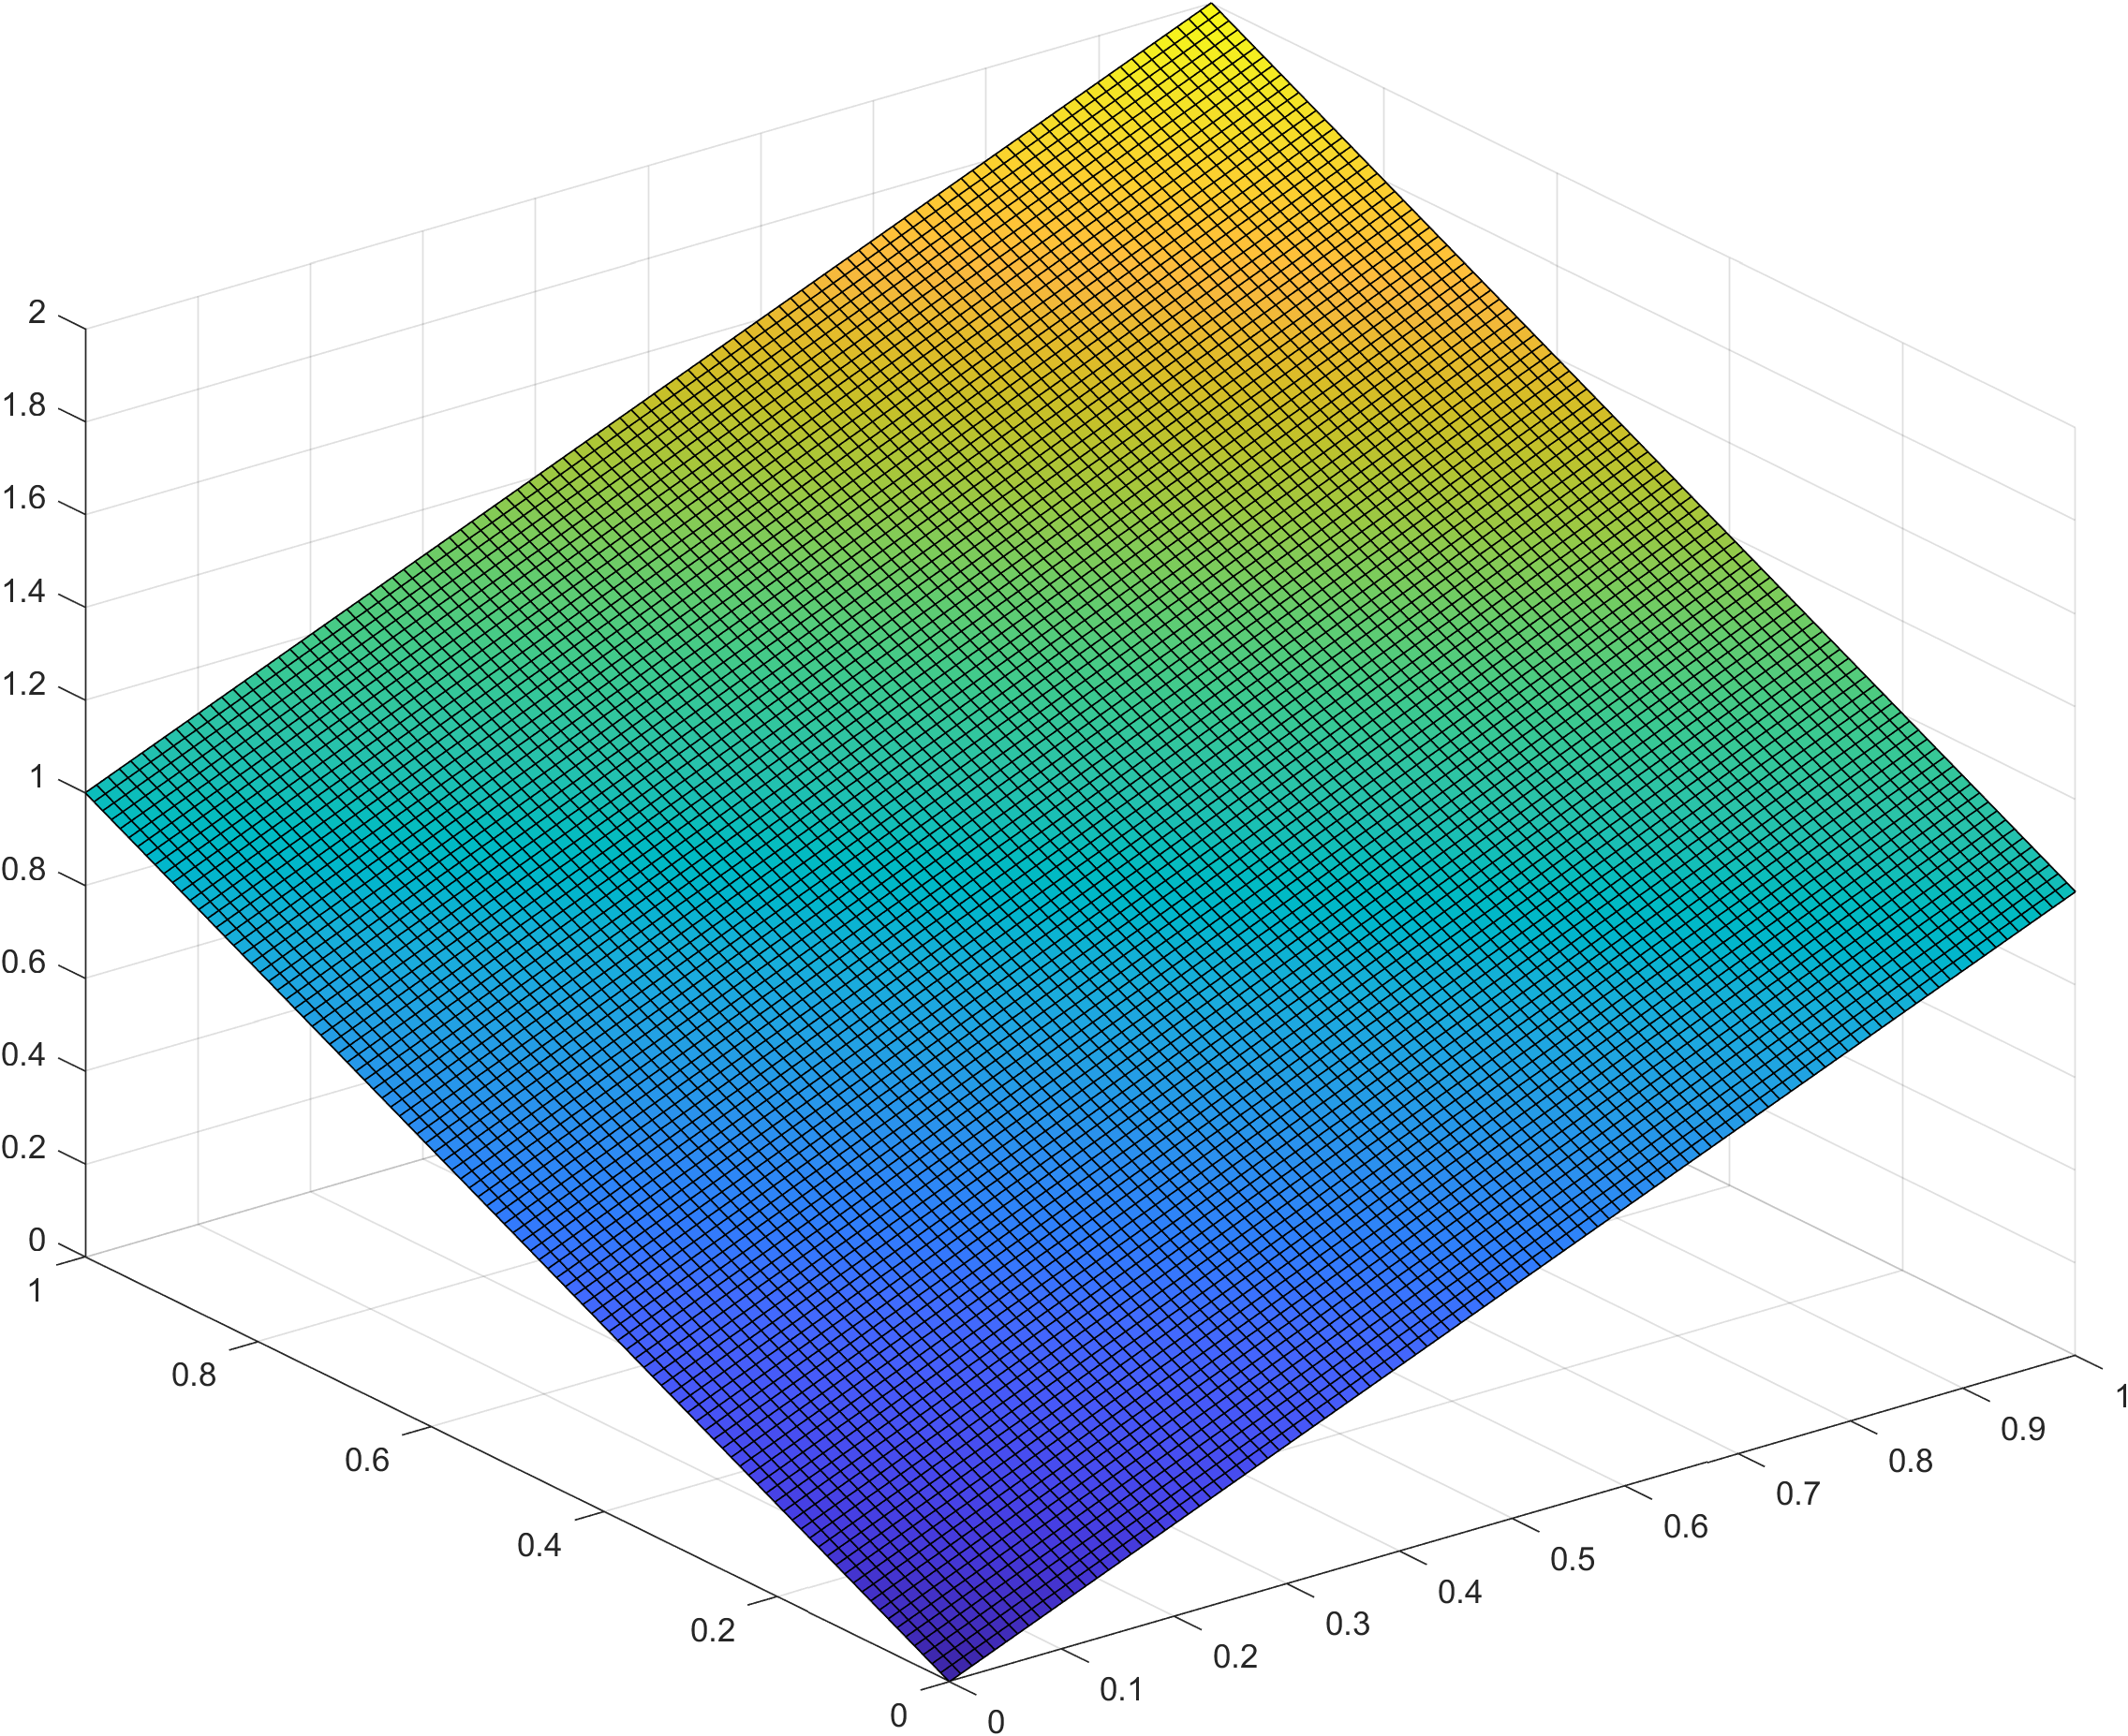
\includegraphics[height=\dimIm]{../Immagini/ET1_SE_NPunti=100_t=0.png}
                            \caption{Soluzione esatta al tempo $t=0$.}
                            \label{figET1TriangolazioniEsattaTI}
                        \end{subfigure}
                        \begin{subfigure}[t]{\lungSF}
                            \centering
                            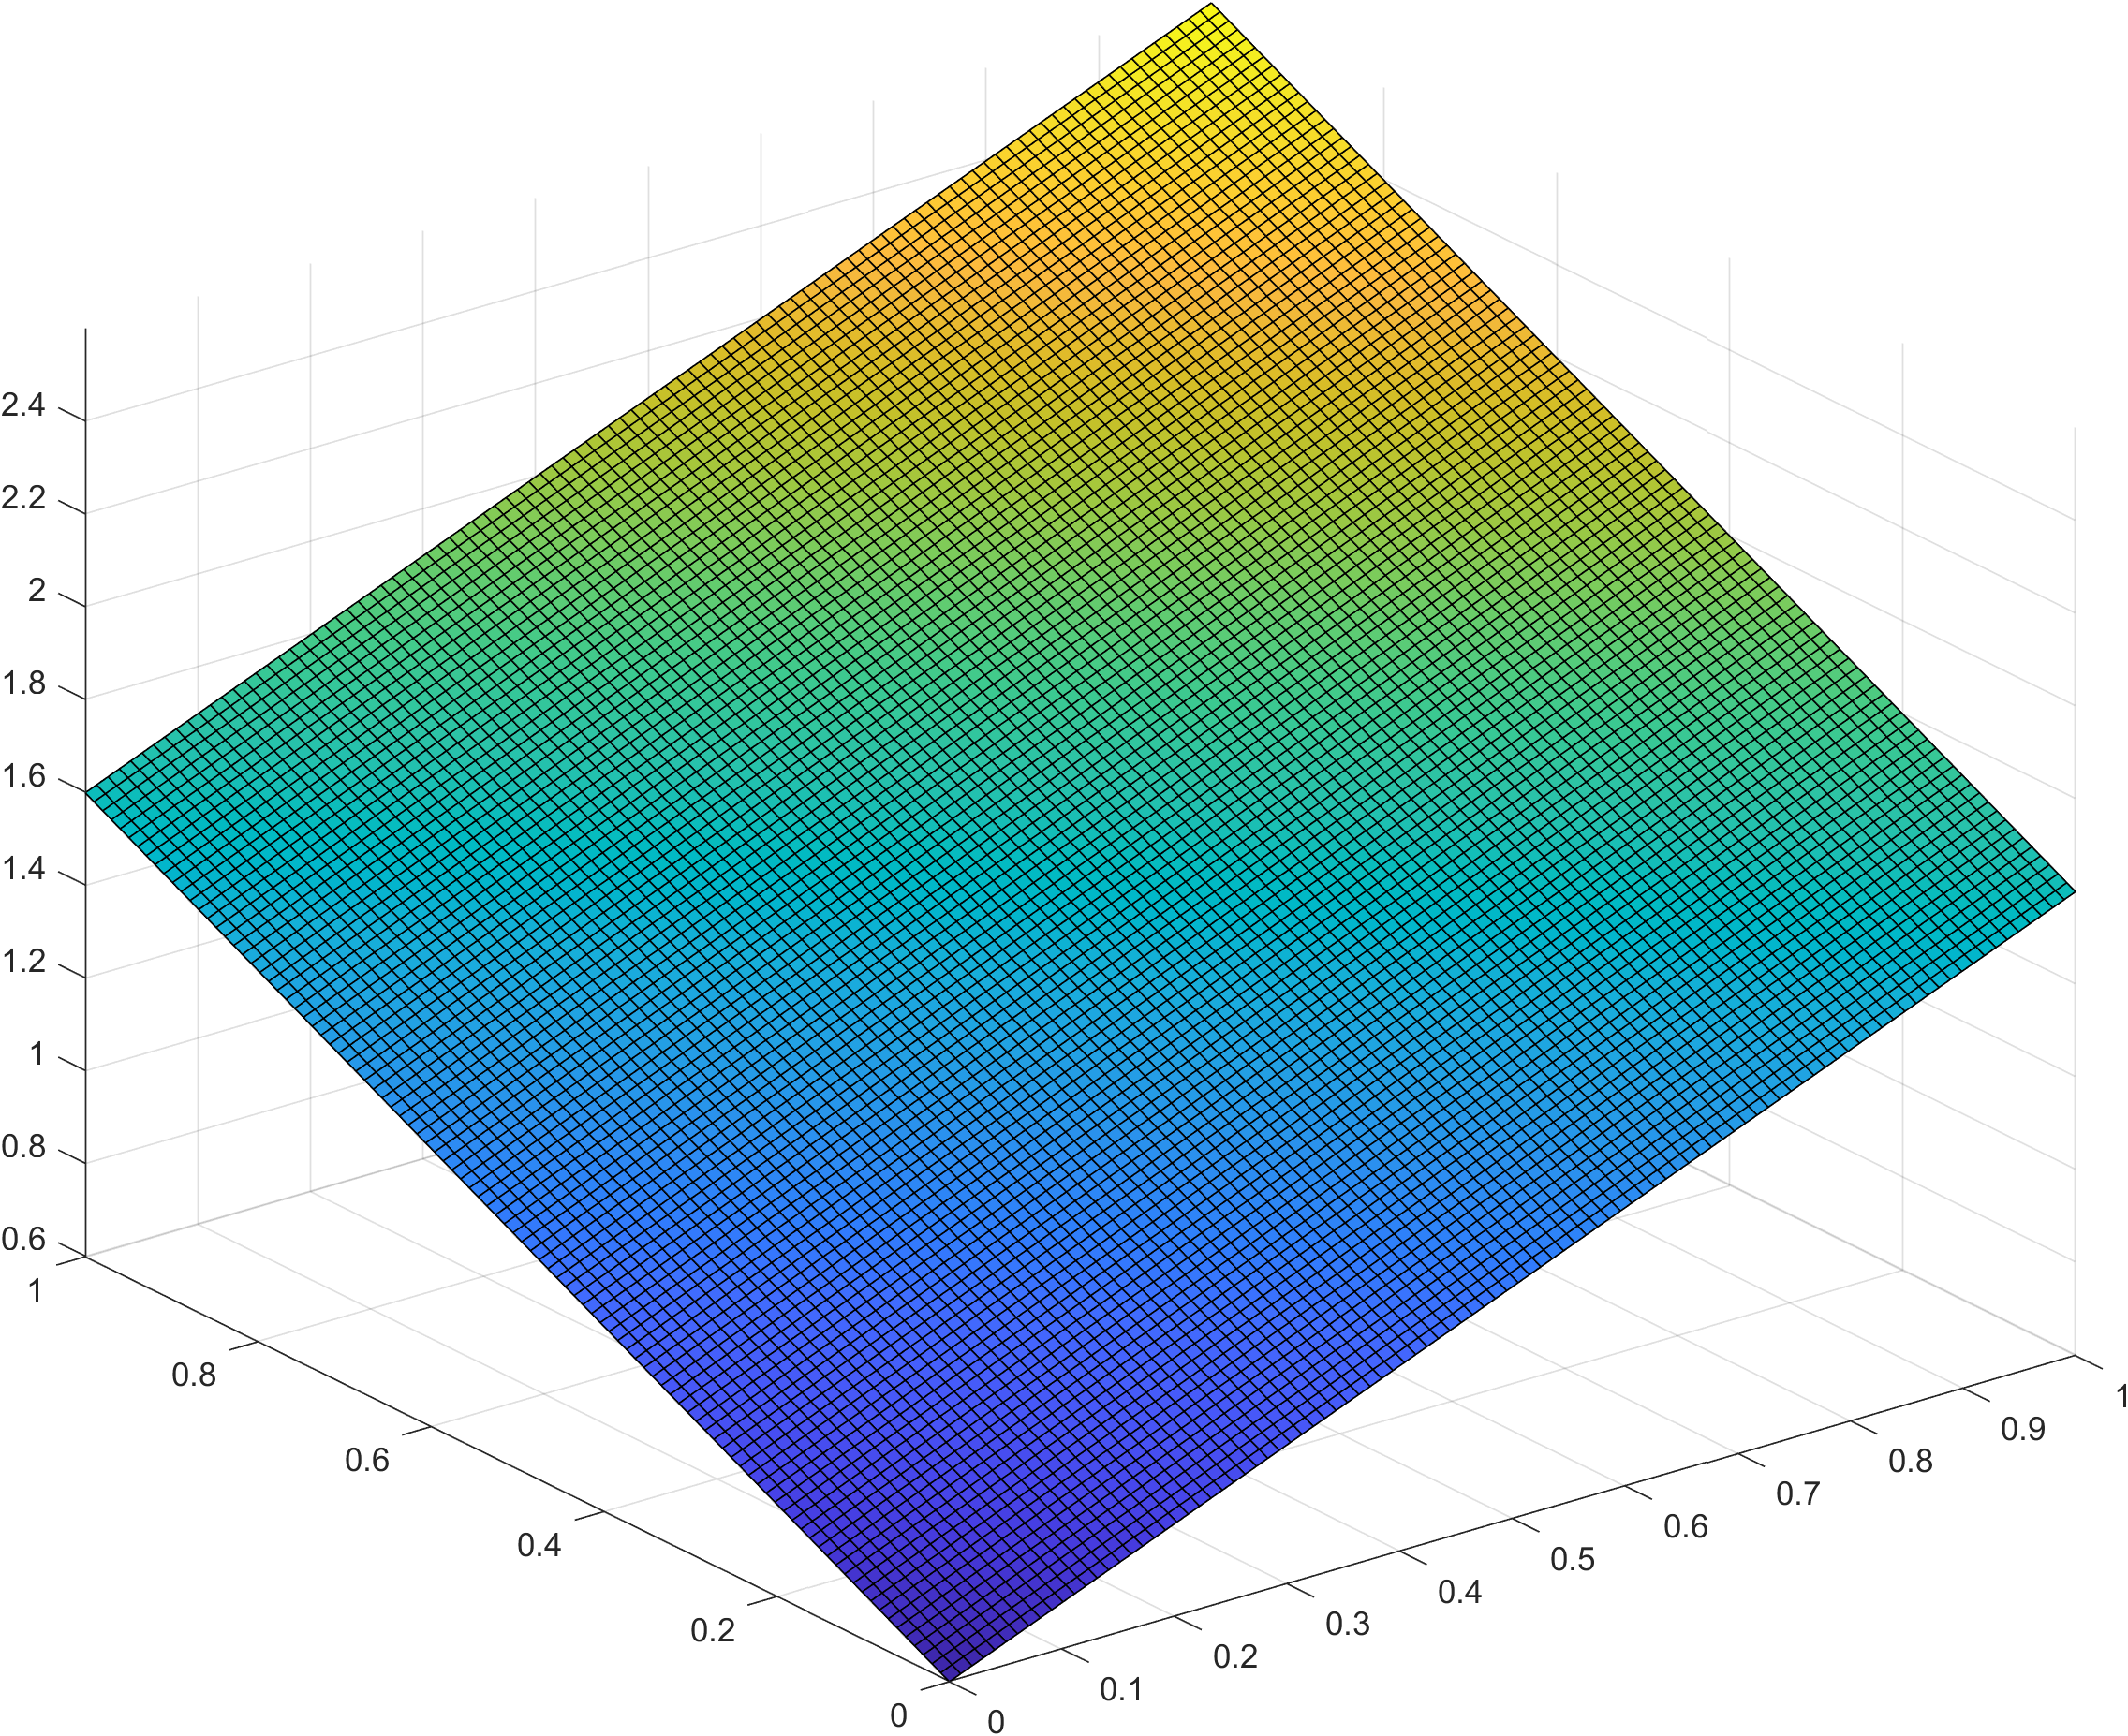
\includegraphics[height=\dimIm]{../Immagini/ET1_SE_NPunti=100_t=0.5.png}
                            \caption{Soluzione esatta al tempo $t=0.5$.}
                            \label{figET1TriangolazioniEsattaTM}
                        \end{subfigure}
                        \begin{subfigure}[t]{\lungSF}
                            \centering
                            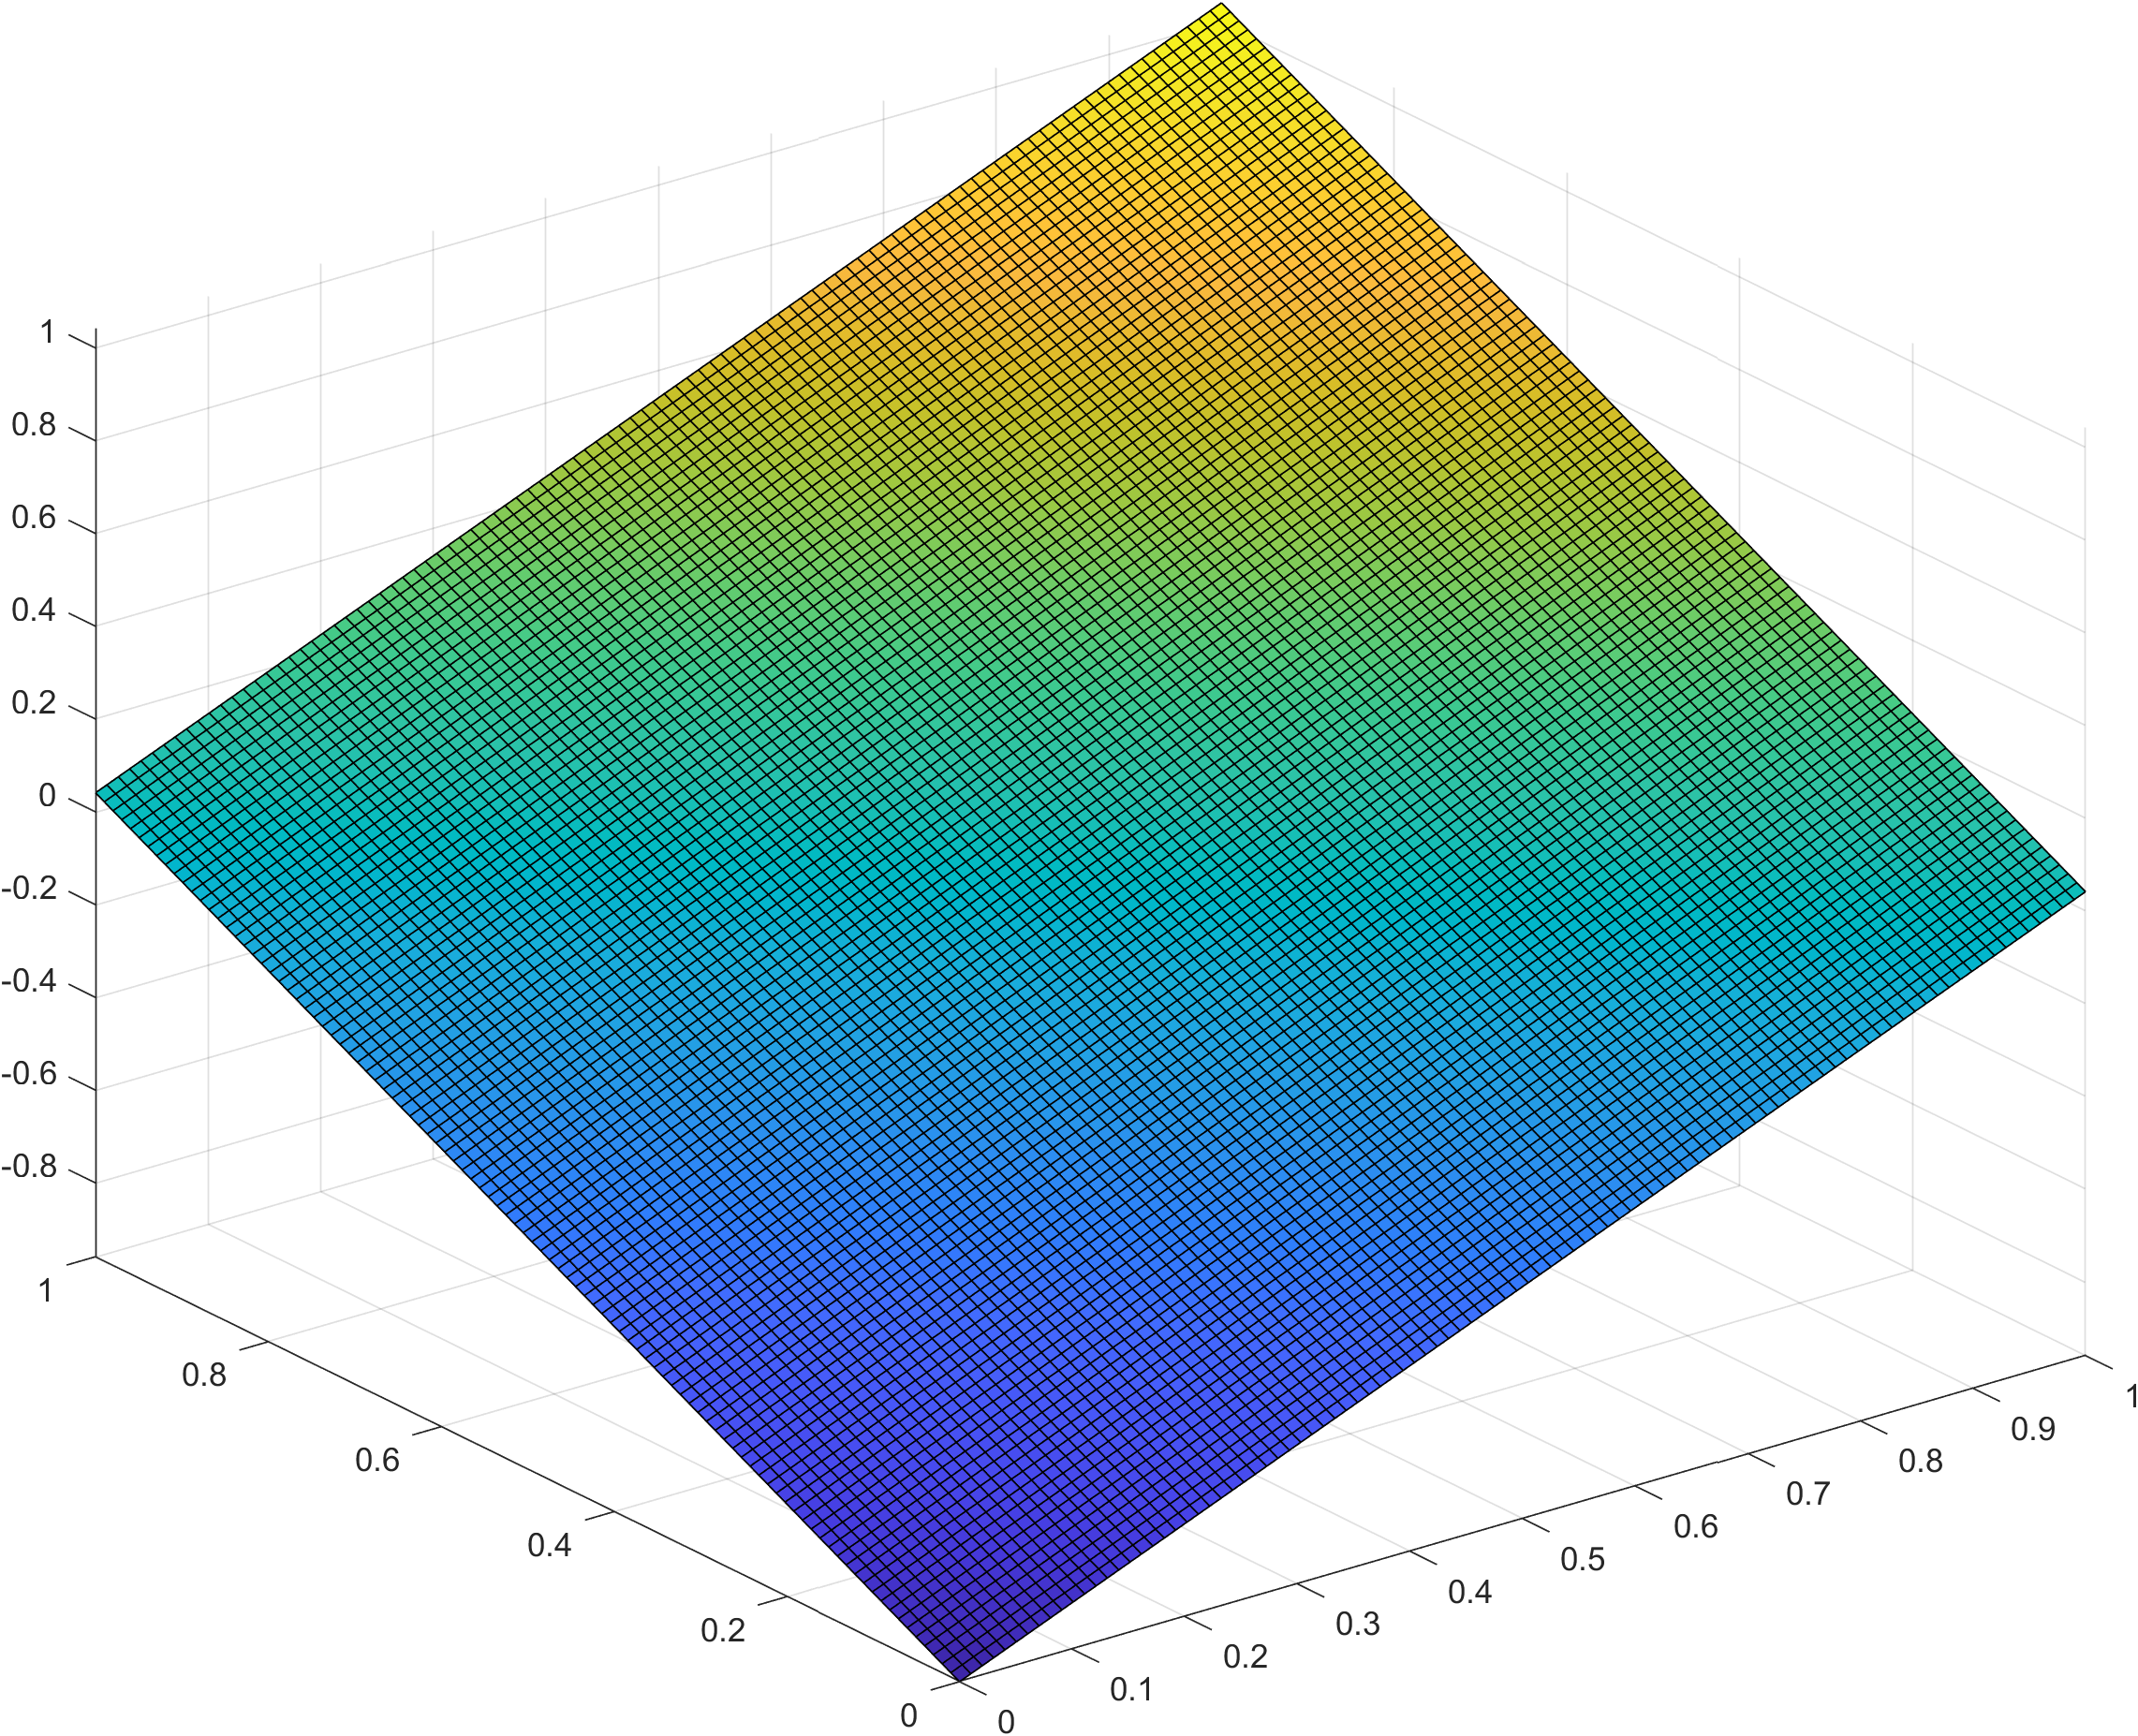
\includegraphics[height=\dimIm]{../Immagini/ET1_SE_NPunti=100_t=1.png}
                            \caption{Soluzione esatta al tempo $t=1$.}
                            \label{figET1TriangolazioniEsattaTF}
                        \end{subfigure}
                    }
                    \distR
                    
                    % \renewcommand{\dimIm}{4cm}
                    \makebox[\linewidth][c]{
                        \captionsetup[subfigure]{width=2.9cm}
                        \SpaziaturaMate{1}{1}{1}
                        \begin{subfigure}[t]{\lungSF}
                            \centering
                            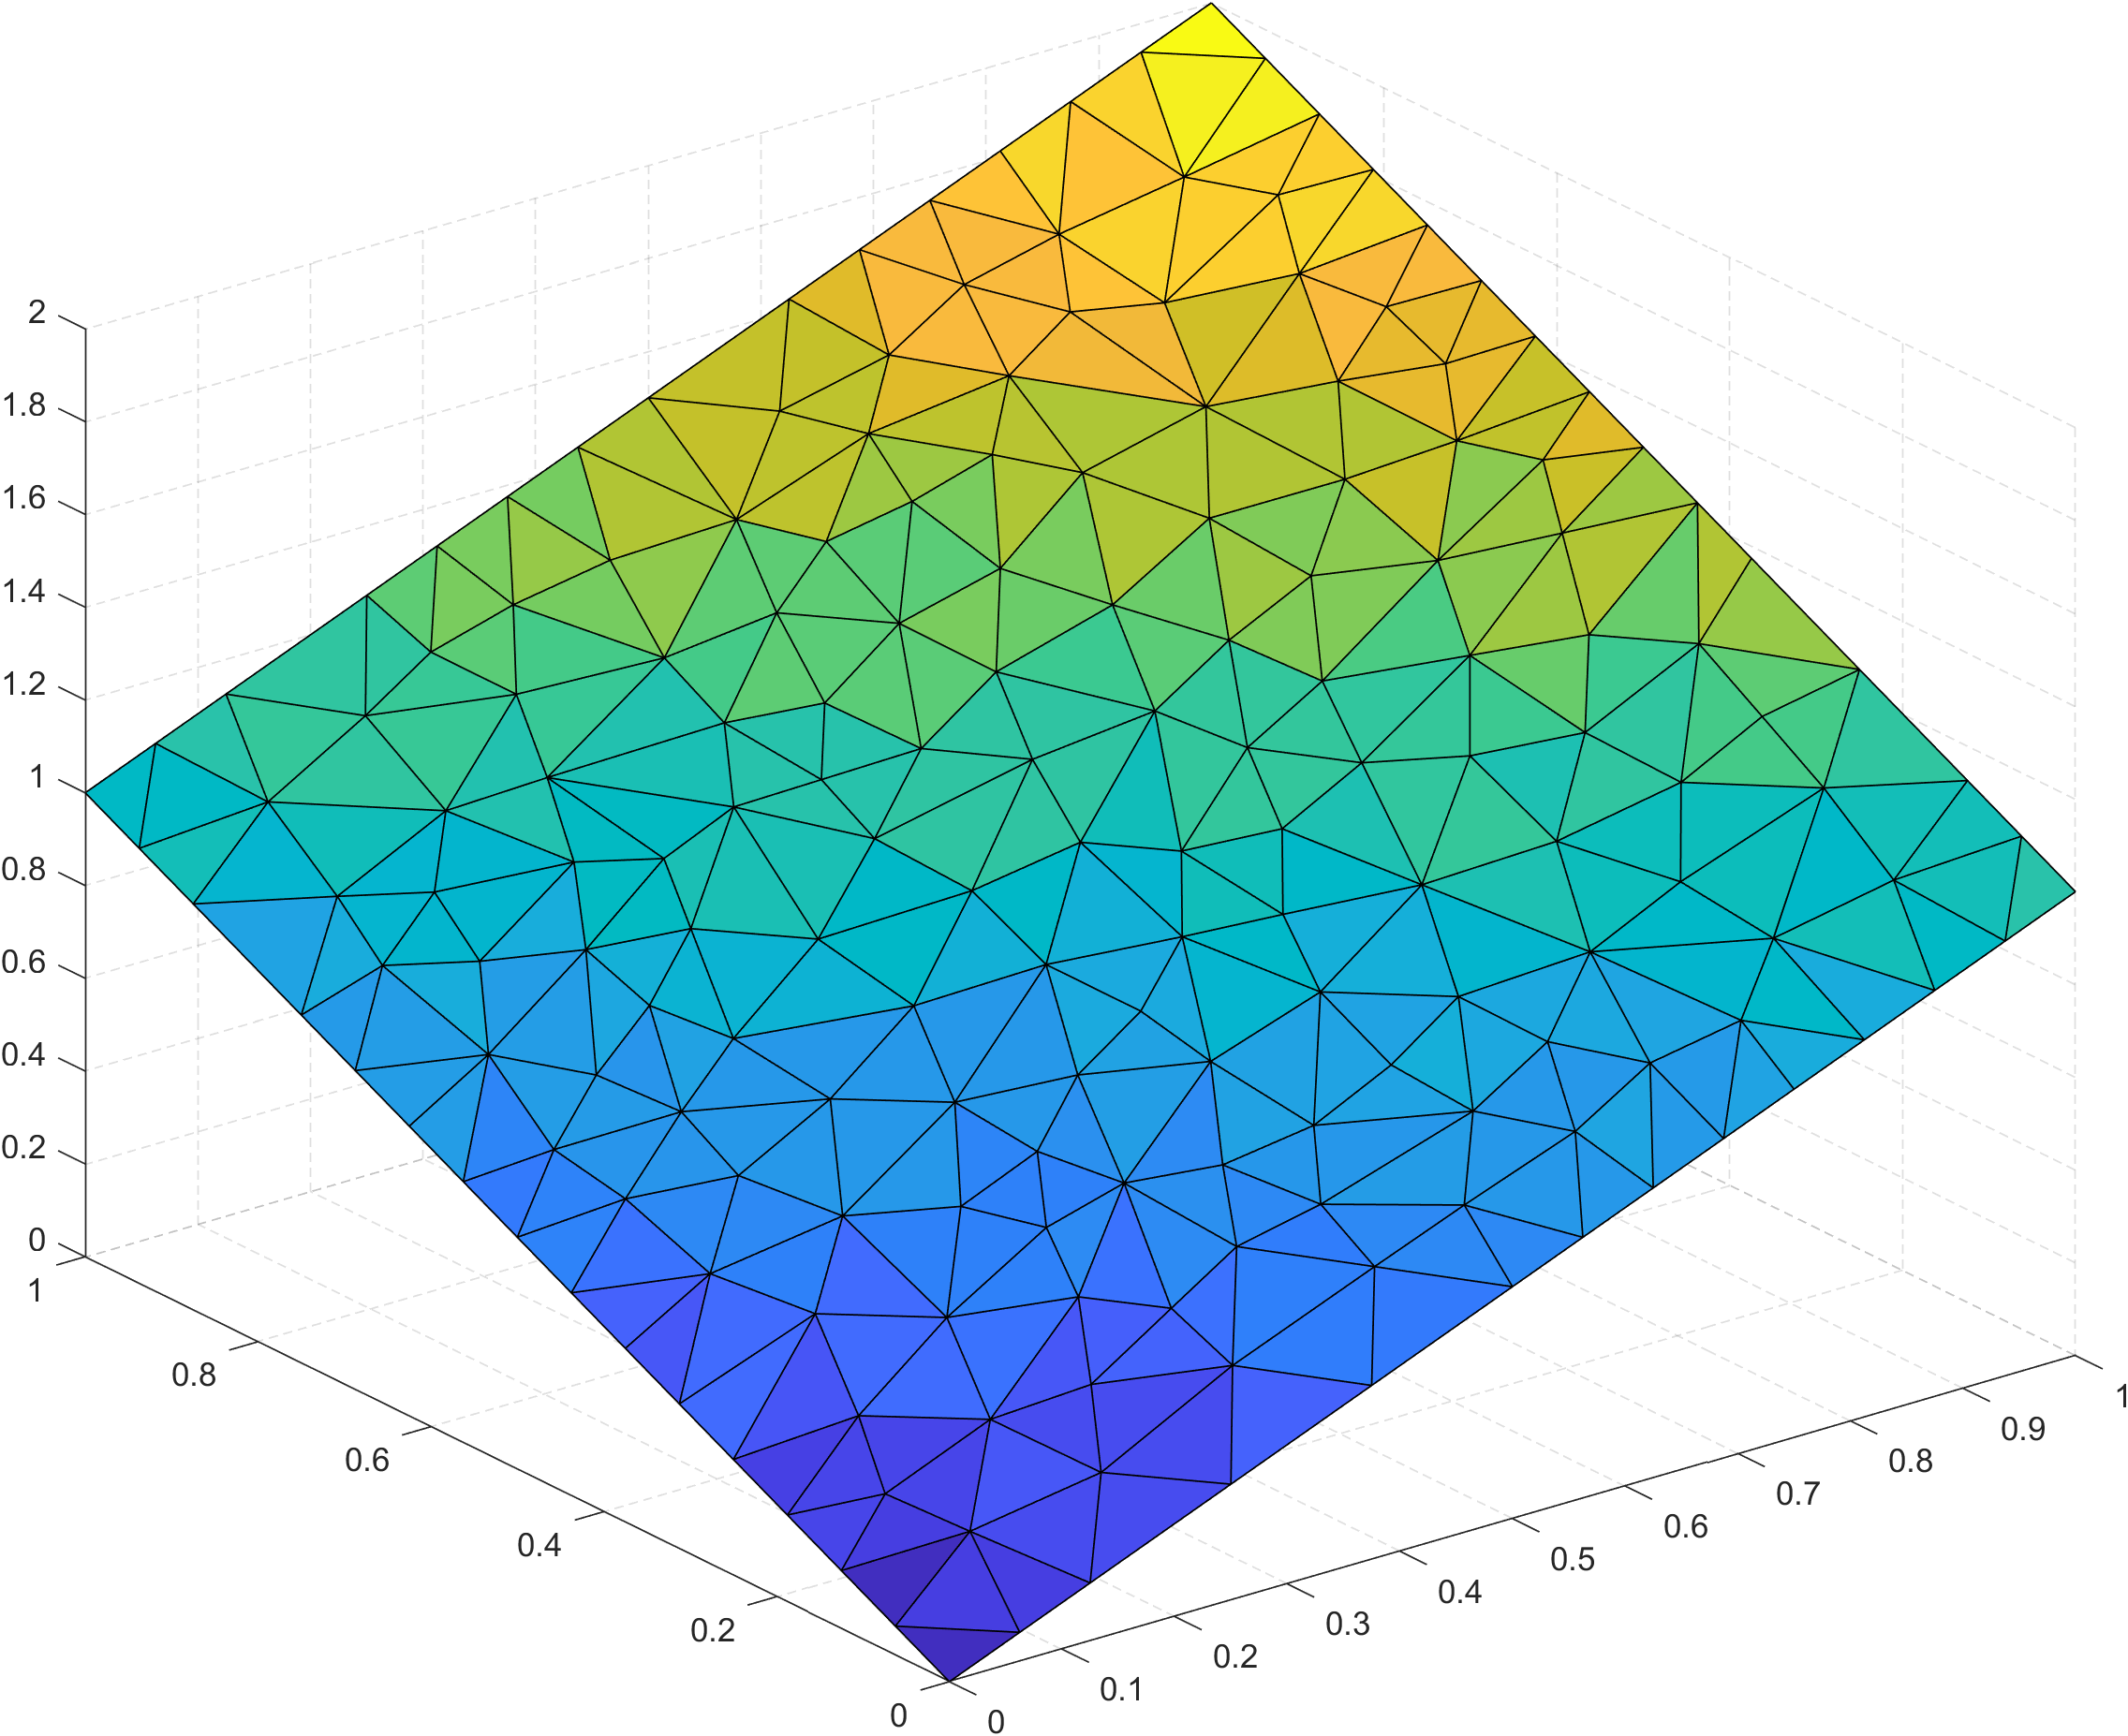
\includegraphics[height=\dimIm]{../Immagini/ET1_P1_AMax=dt=0.005_t=0.png}
                            \caption{Soluzione qualitativa coi $\mathbb{P}_1$ al tempo $t=0$.}
                            \label{figET1TriangolazioniP1TI}
                        \end{subfigure}
                        \begin{subfigure}[t]{\lungSF}
                            \centering
                            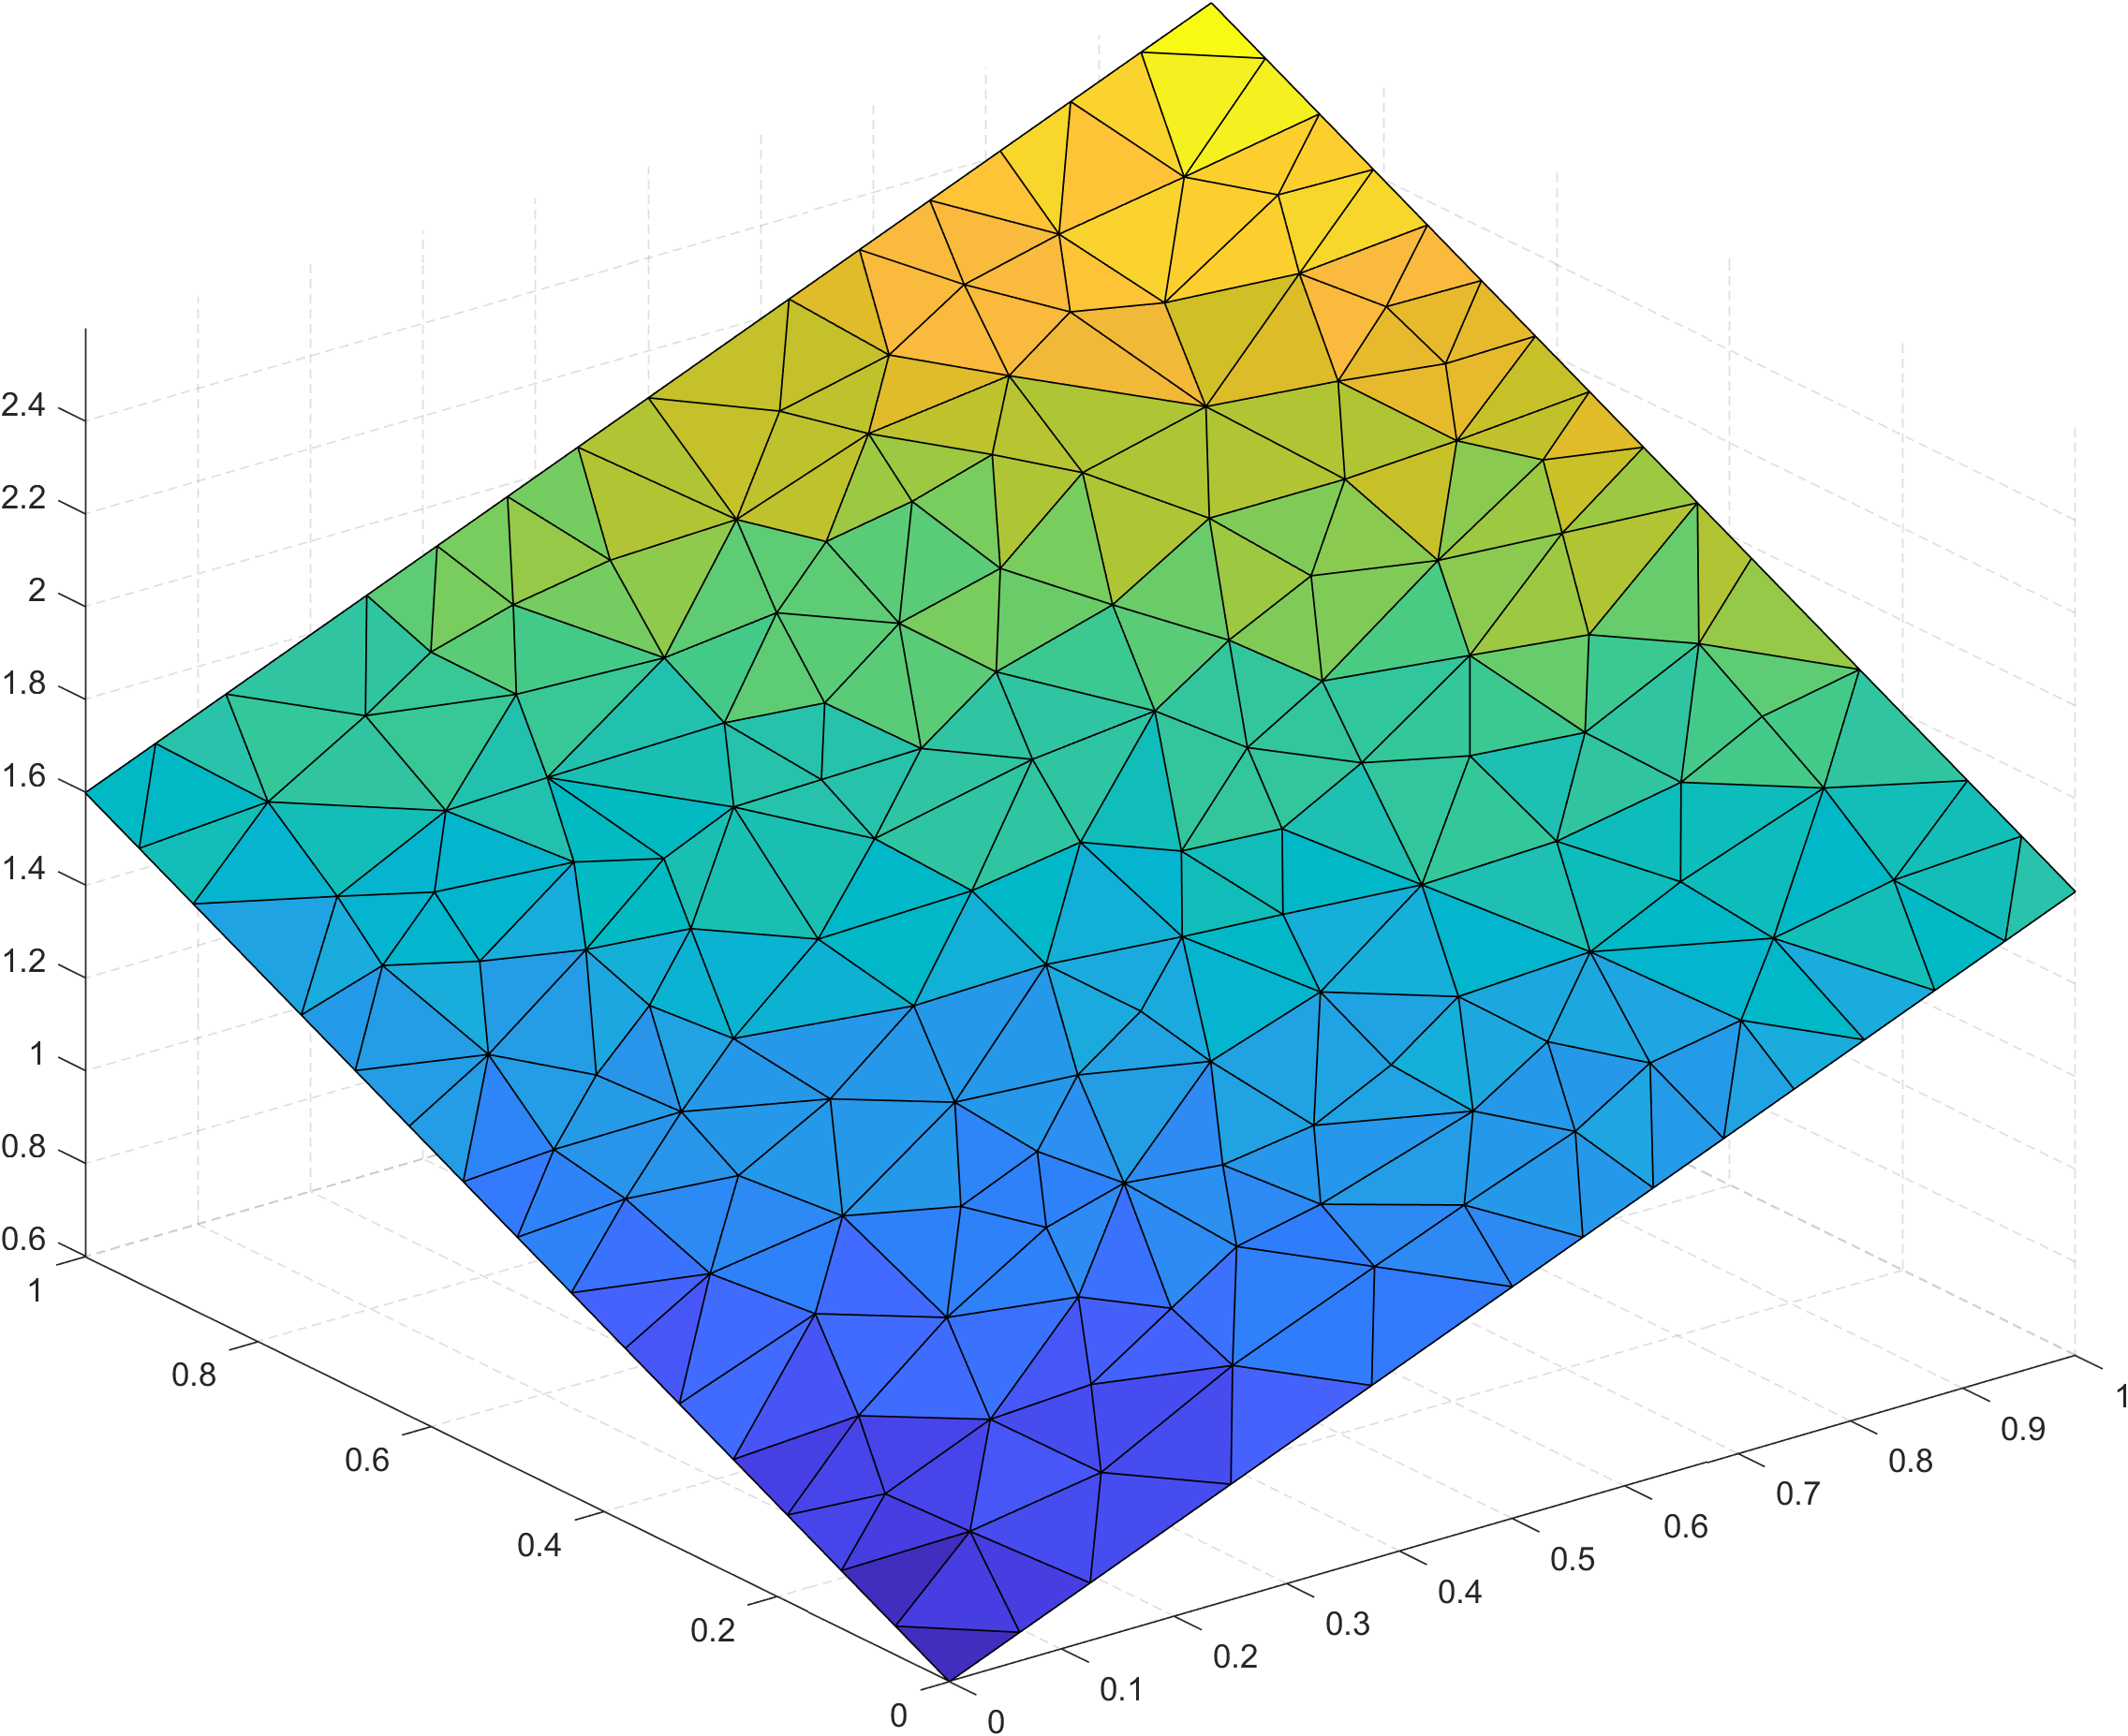
\includegraphics[height=\dimIm]{../Immagini/ET1_P1_AMax=dt=0.005_t=0.5.png}
                            \caption{Soluzione qualitativa coi $\mathbb{P}_1$ al tempo $t=0.5$.}
                            \label{figET1TriangolazioniP1TM}
                        \end{subfigure}
                        \begin{subfigure}[t]{\lungSF}
                            \centering
                            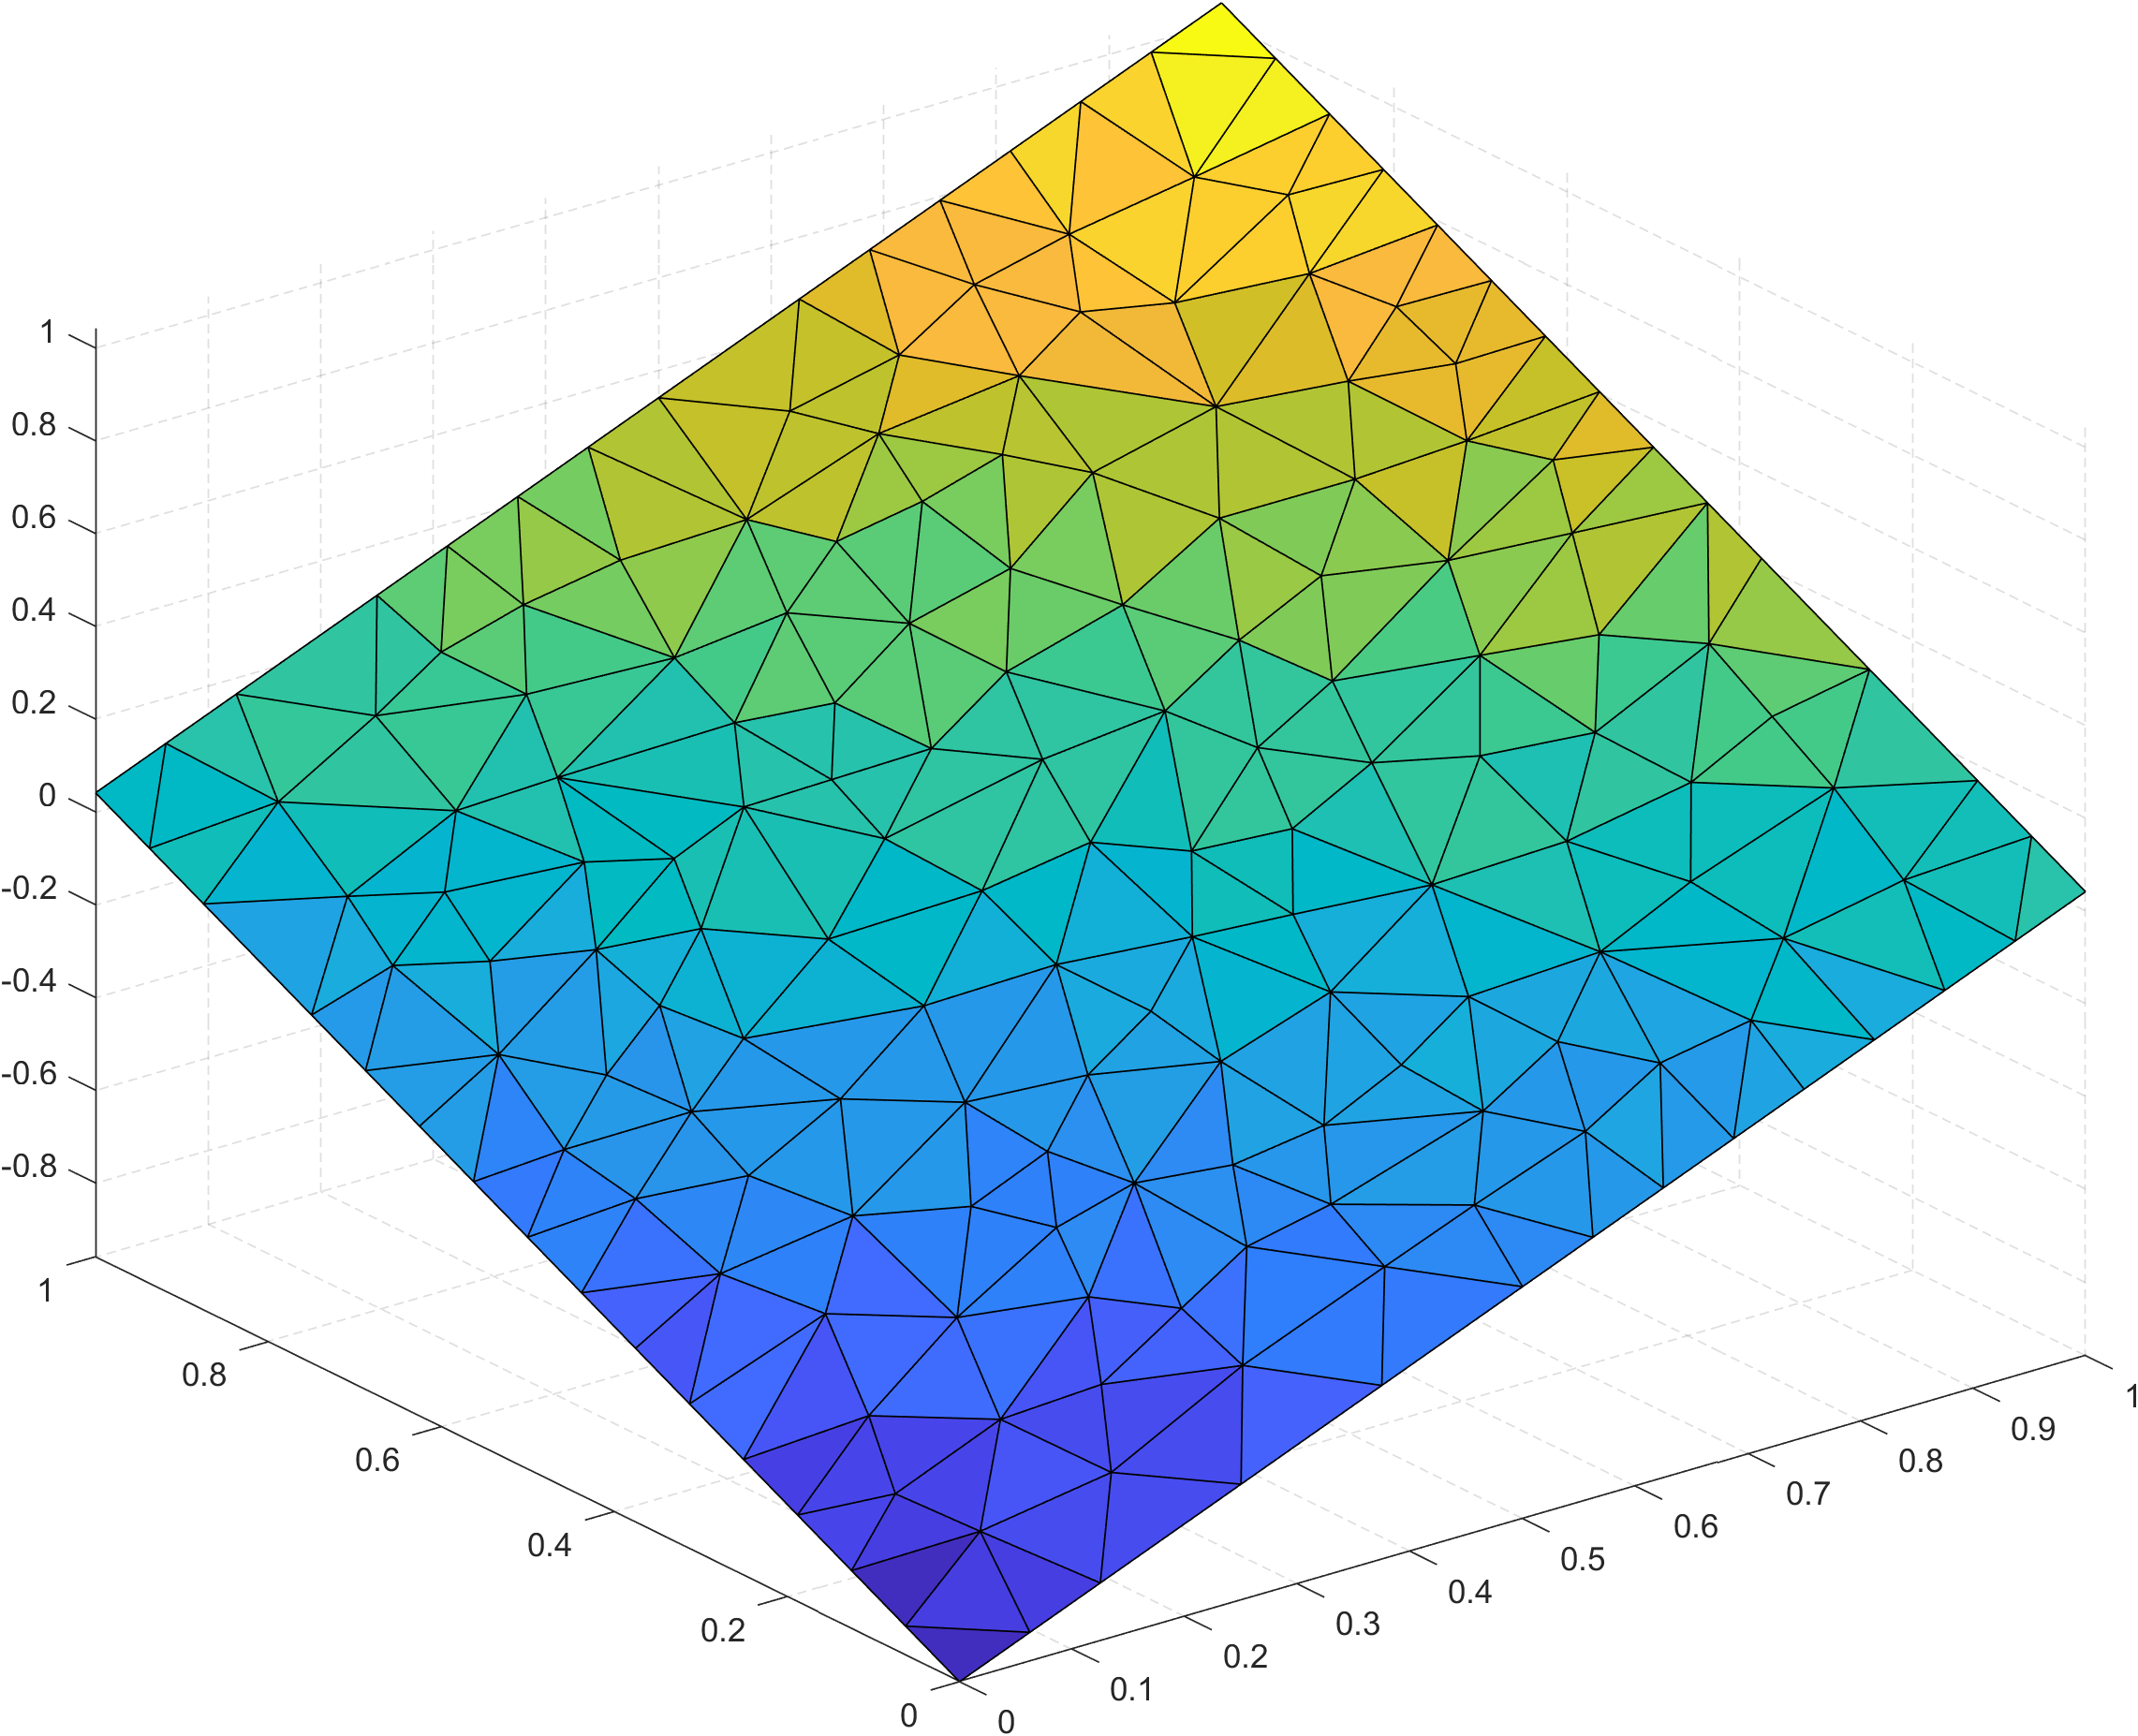
\includegraphics[height=\dimIm]{../Immagini/ET1_P1_AMax=dt=0.005_t=1.png}
                            \caption{Soluzione qualitativa coi $\mathbb{P}_1$ al tempo $t=1$.}
                            \label{figET1TriangolazioniP1TF}
                        \end{subfigure}
                    }
                    \distR
        
                    \renewcommand{\lungSF}{.5\linewidth}
                    \renewcommand{\dimIm}{\linewidth}
                    \newcommand{\distC}{\hspace{7.5pt}} % Distanza tra le colonne
                    \makebox[\linewidth][c]{
                        \begin{subfigure}[c]{\lungSF}
                            \centering
                            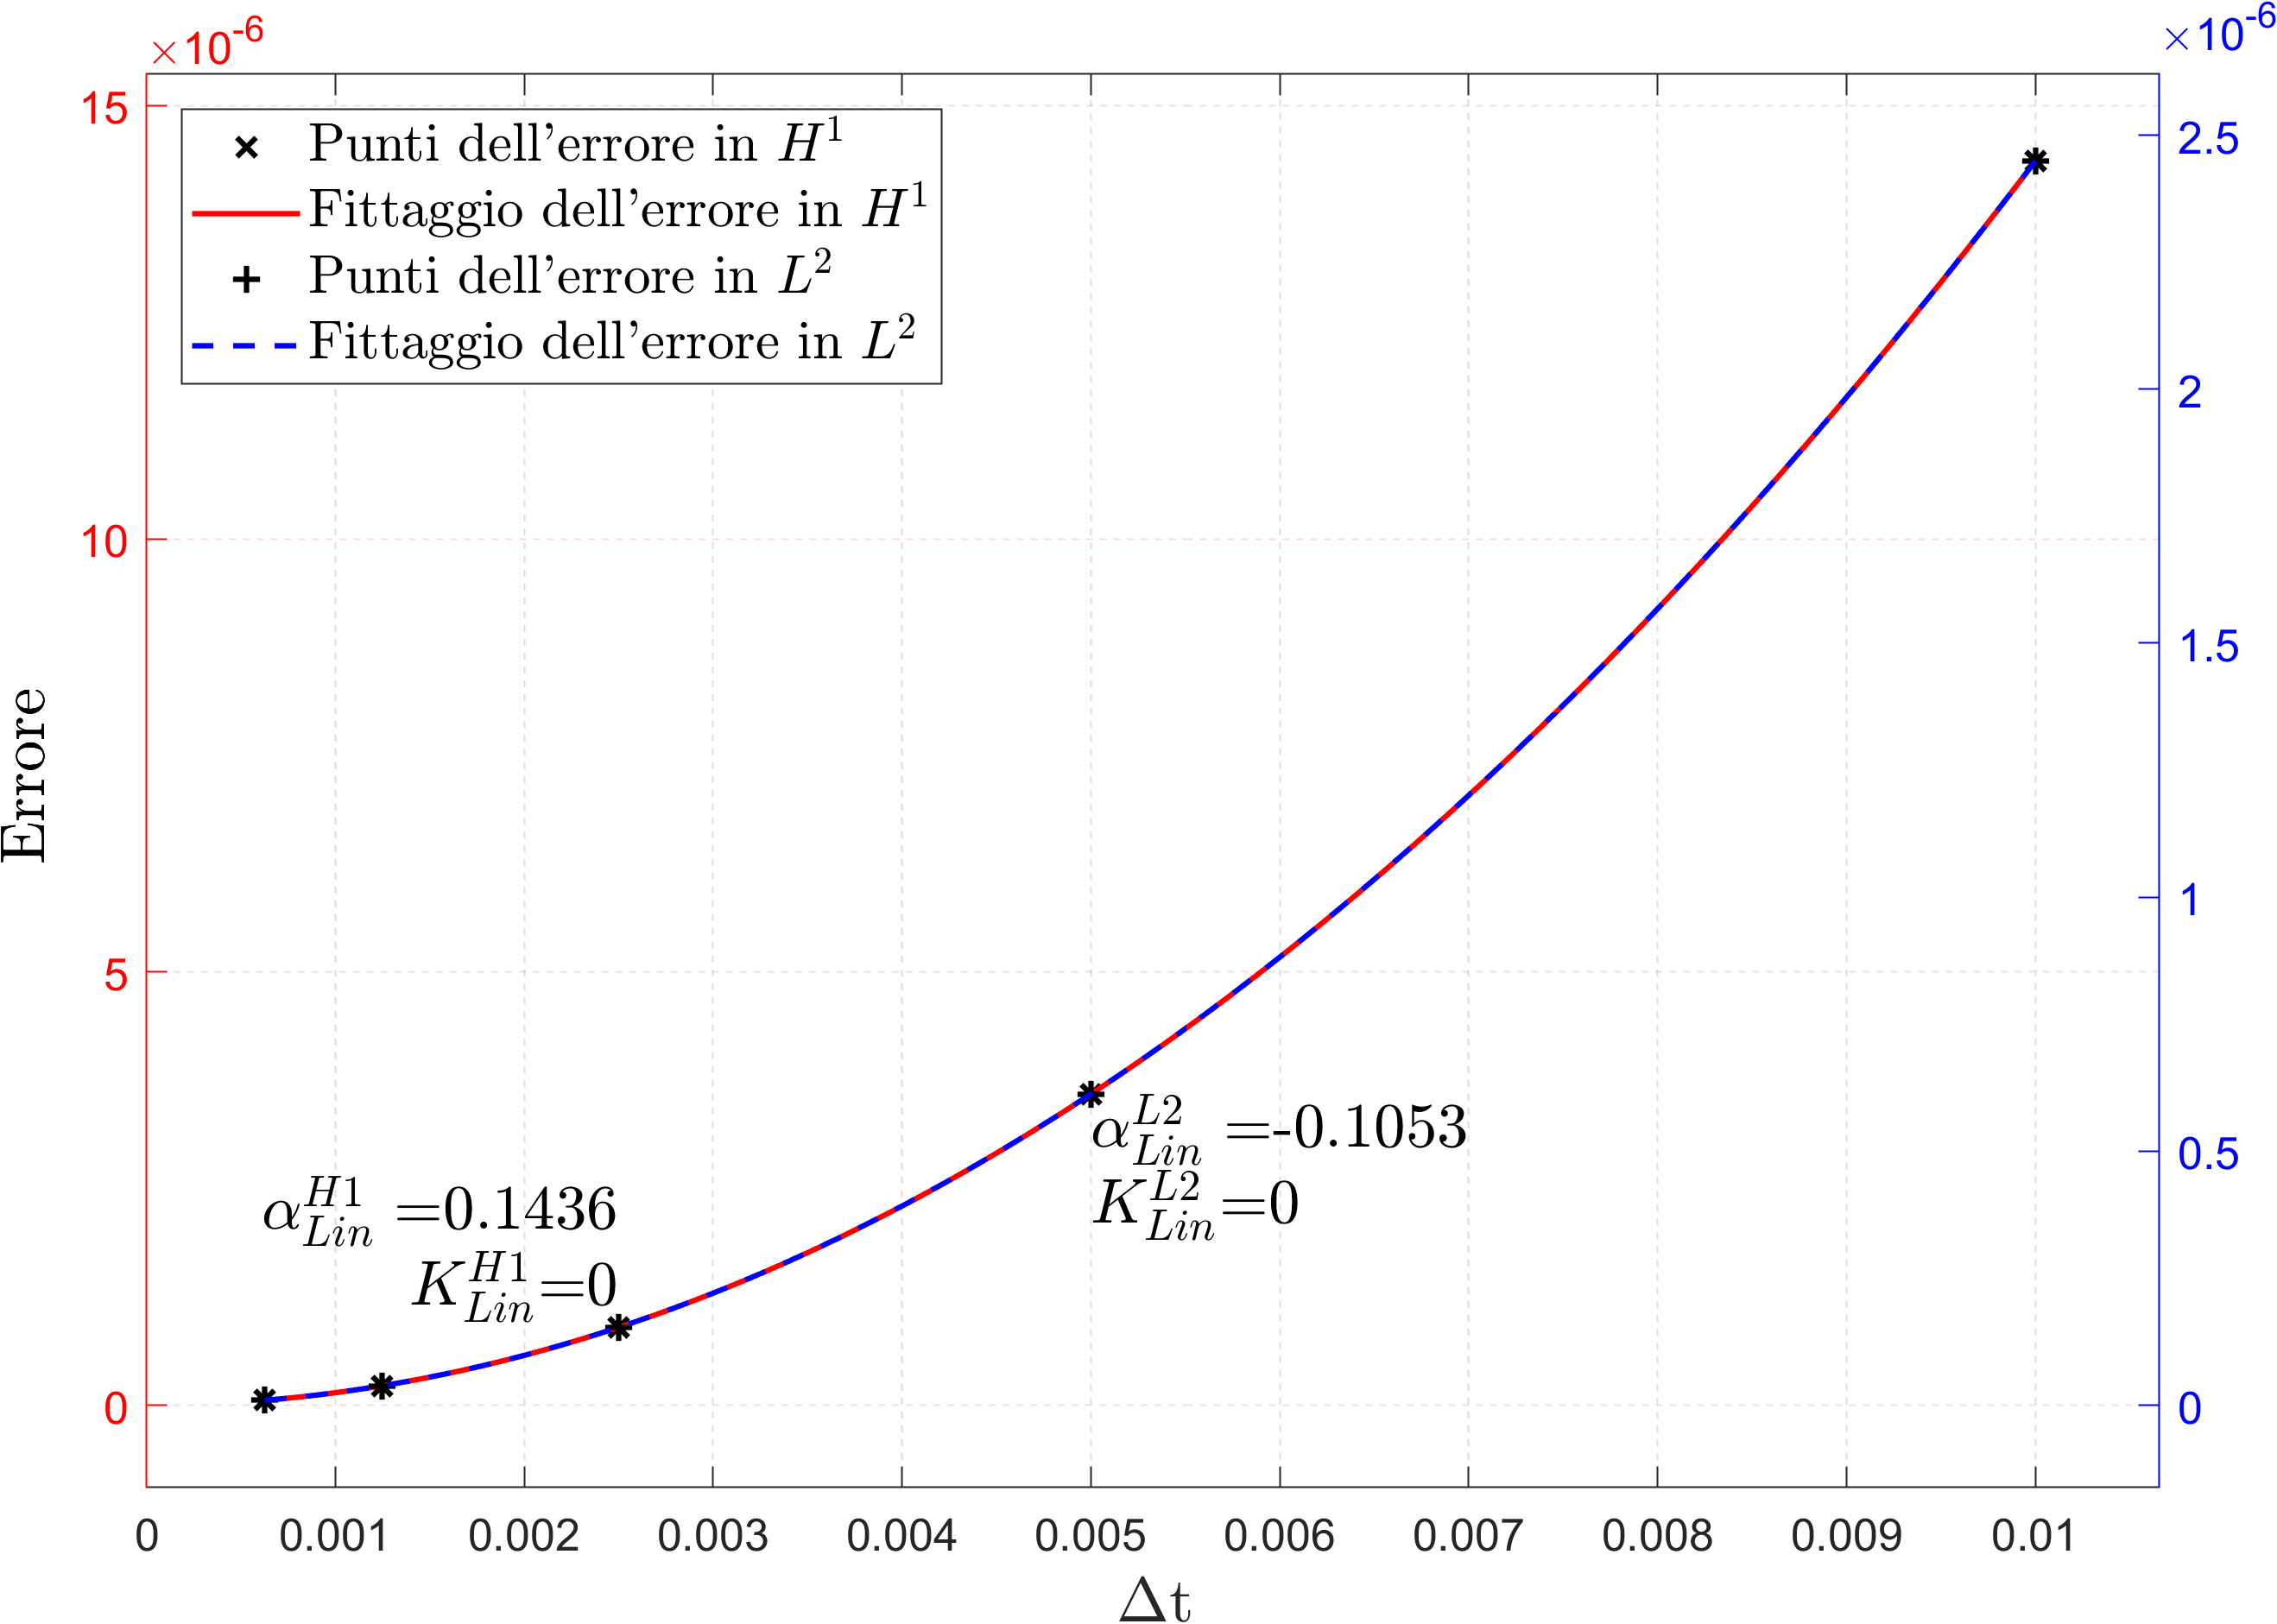
\includegraphics[width=\dimIm]{../Immagini/ET1_P1_ErrLin_AMax=dt=0.01_NSim=5.png}
                        \caption{Errore dei $\mathbb{P}_1$ in scala lineare.}
                        \label{figET1ErroreP1Lin}
                        \end{subfigure}
                        \distC
                        \begin{subfigure}[c]{\lungSF}
                            \centering
                            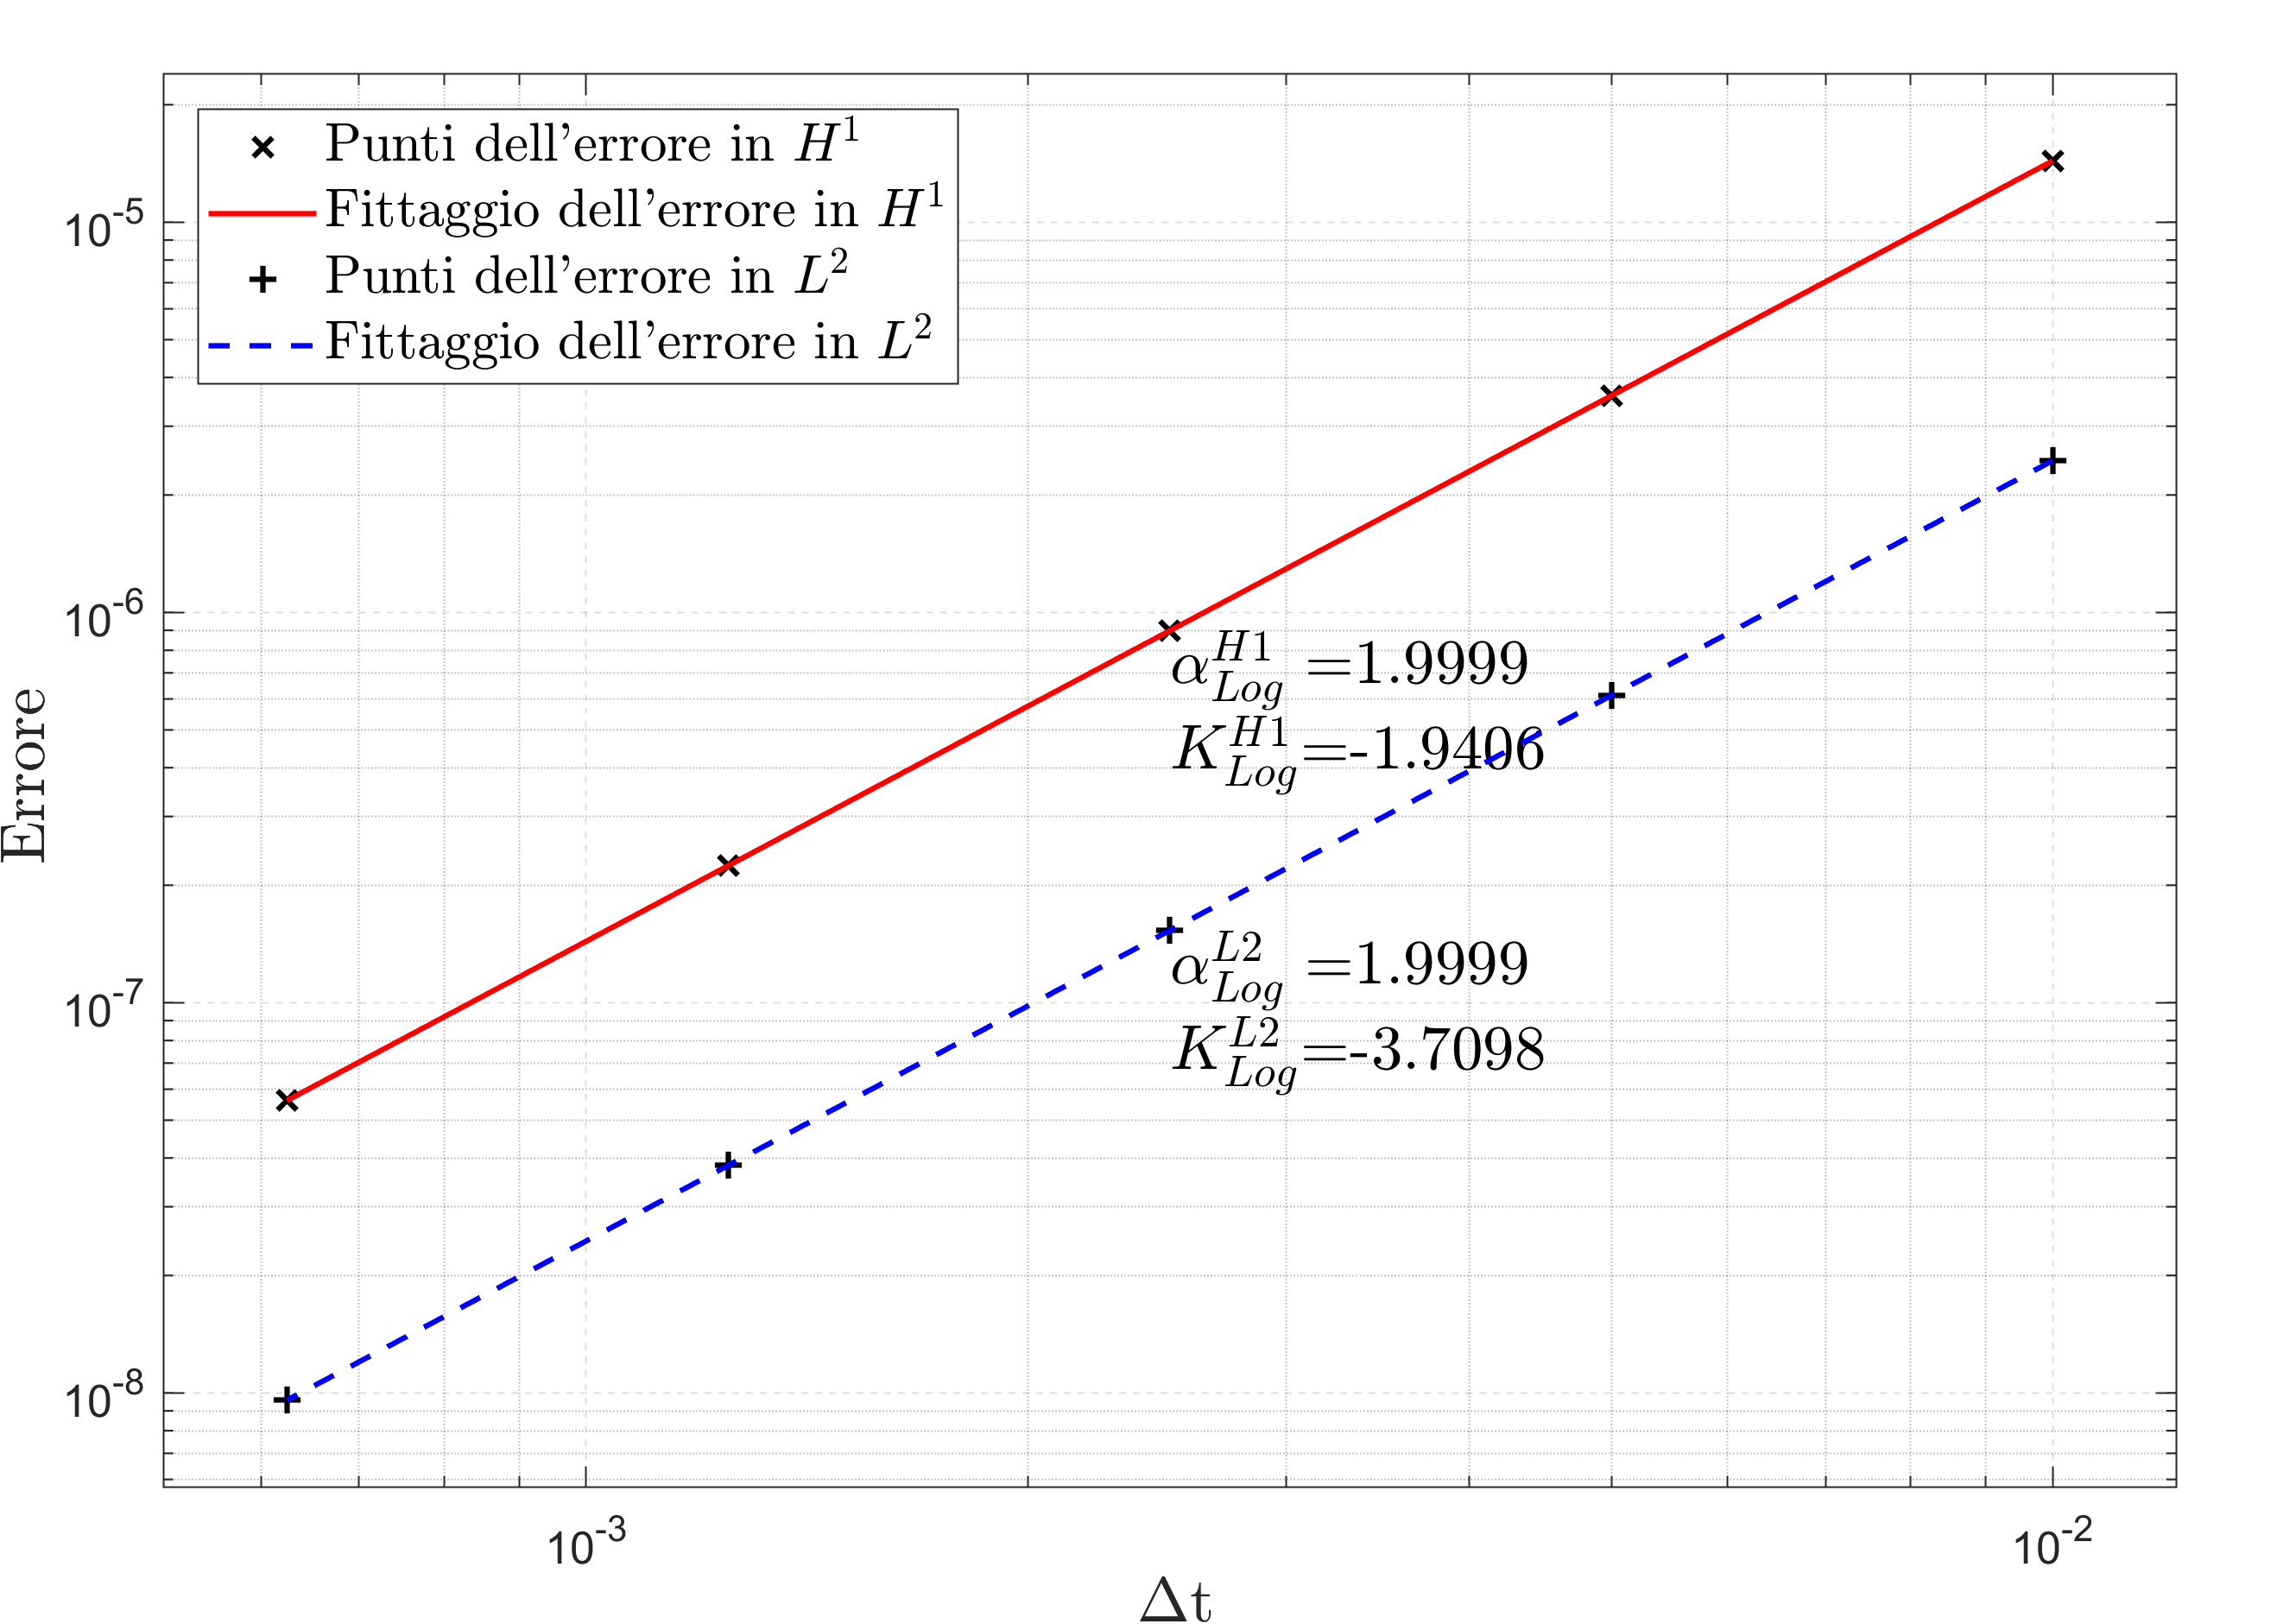
\includegraphics[width=\dimIm]{../Immagini/ET1_P1_ErrLog_AMax=dt=0.01_NSim=5.png}
                        \caption{Errore dei $\mathbb{P}_1$ in scala logaritmica.}
                        \label{figET1ErroreP1Log}
                        \end{subfigure}
                    }
                    \caption{Nelle Figg. \ref{figET1TriangolazioniEsattaTI}-\ref{figET1TriangolazioniP1TF} sono mostrate le soluzioni dell'ET1 in tre istanti temporali: le prime tre mostrano la soluzione esatta e le restanti quella approssimata; invece nelle \ref{figET1ErroreP1Lin} e \ref{figET1ErroreP1Log} sono illustrati in due scale diverse gli errori in norma $H^1$ ed $L^2$. I parametri dati a \textit{BBTR} sono spiegati nel $\S$\ref{parPremessaParametriBBTR}.}
                    \label{figET1}
                \end{figure*}
                %%%%%%%%%%%%%%%%%%
                %%%%%%%%%%%%%%%%%%
                %%%%%%%%%%%%%%%%%%

                %%%%%%%%%%%%%%%%%%%%%%
                %%% Infopagina ET2 %%%
                %%%%%%%%%%%%%%%%%%%%%%
                \begin{figure*}[p]
                    \newcommand{\distR}{\vspace{15pt}} % Distanza tra le righe
                    
                    \newcommand{\lungSF}{0.33\textwidth}
                    \newcommand{\dimIm}{4.6cm}
                    \makebox[\linewidth][c]{
                        % \captionsetup[subfigure]{width=2.4cm}
                        \SpaziaturaMate{1}{1}{1}
                        \begin{subfigure}[t]{\lungSF}
                            \centering
                            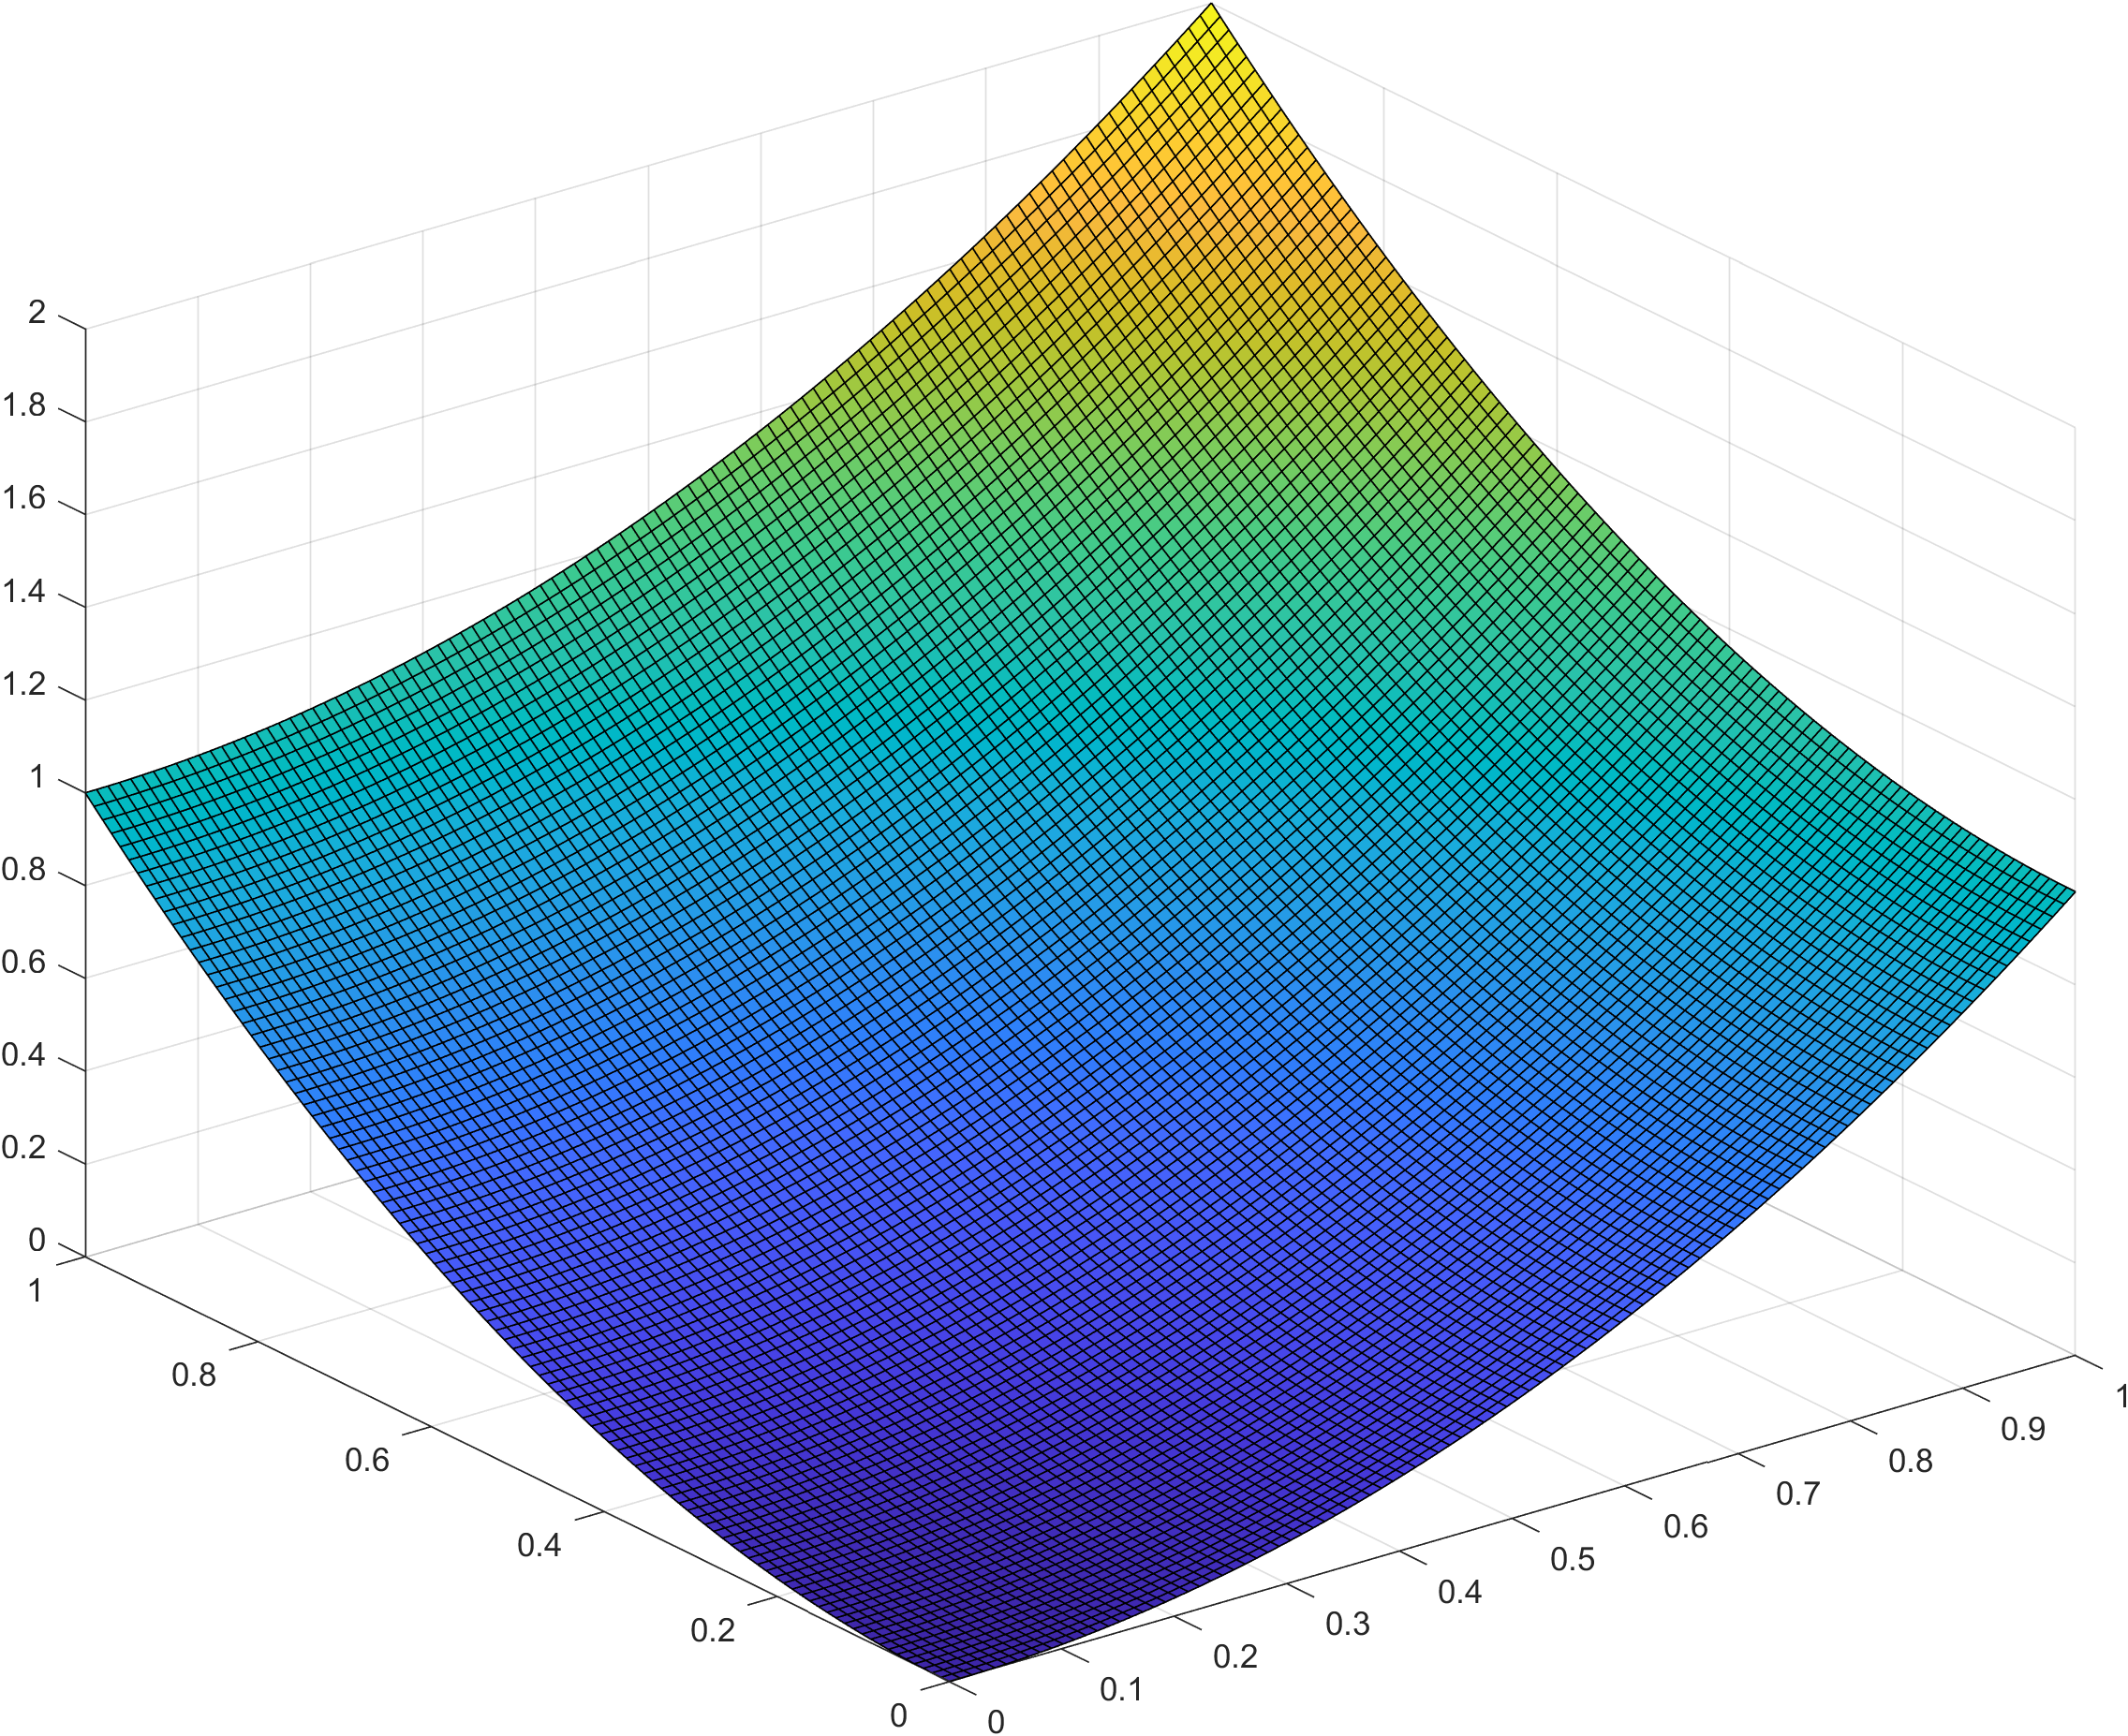
\includegraphics[height=\dimIm]{../Immagini/ET2_SE_NPunti=100_t=0.png}
                            \caption{Soluzione esatta al tempo $t=0$.}
                            \label{figET2TriangolazioniEsattaTI}
                        \end{subfigure}
                        \begin{subfigure}[t]{\lungSF}
                            \centering
                            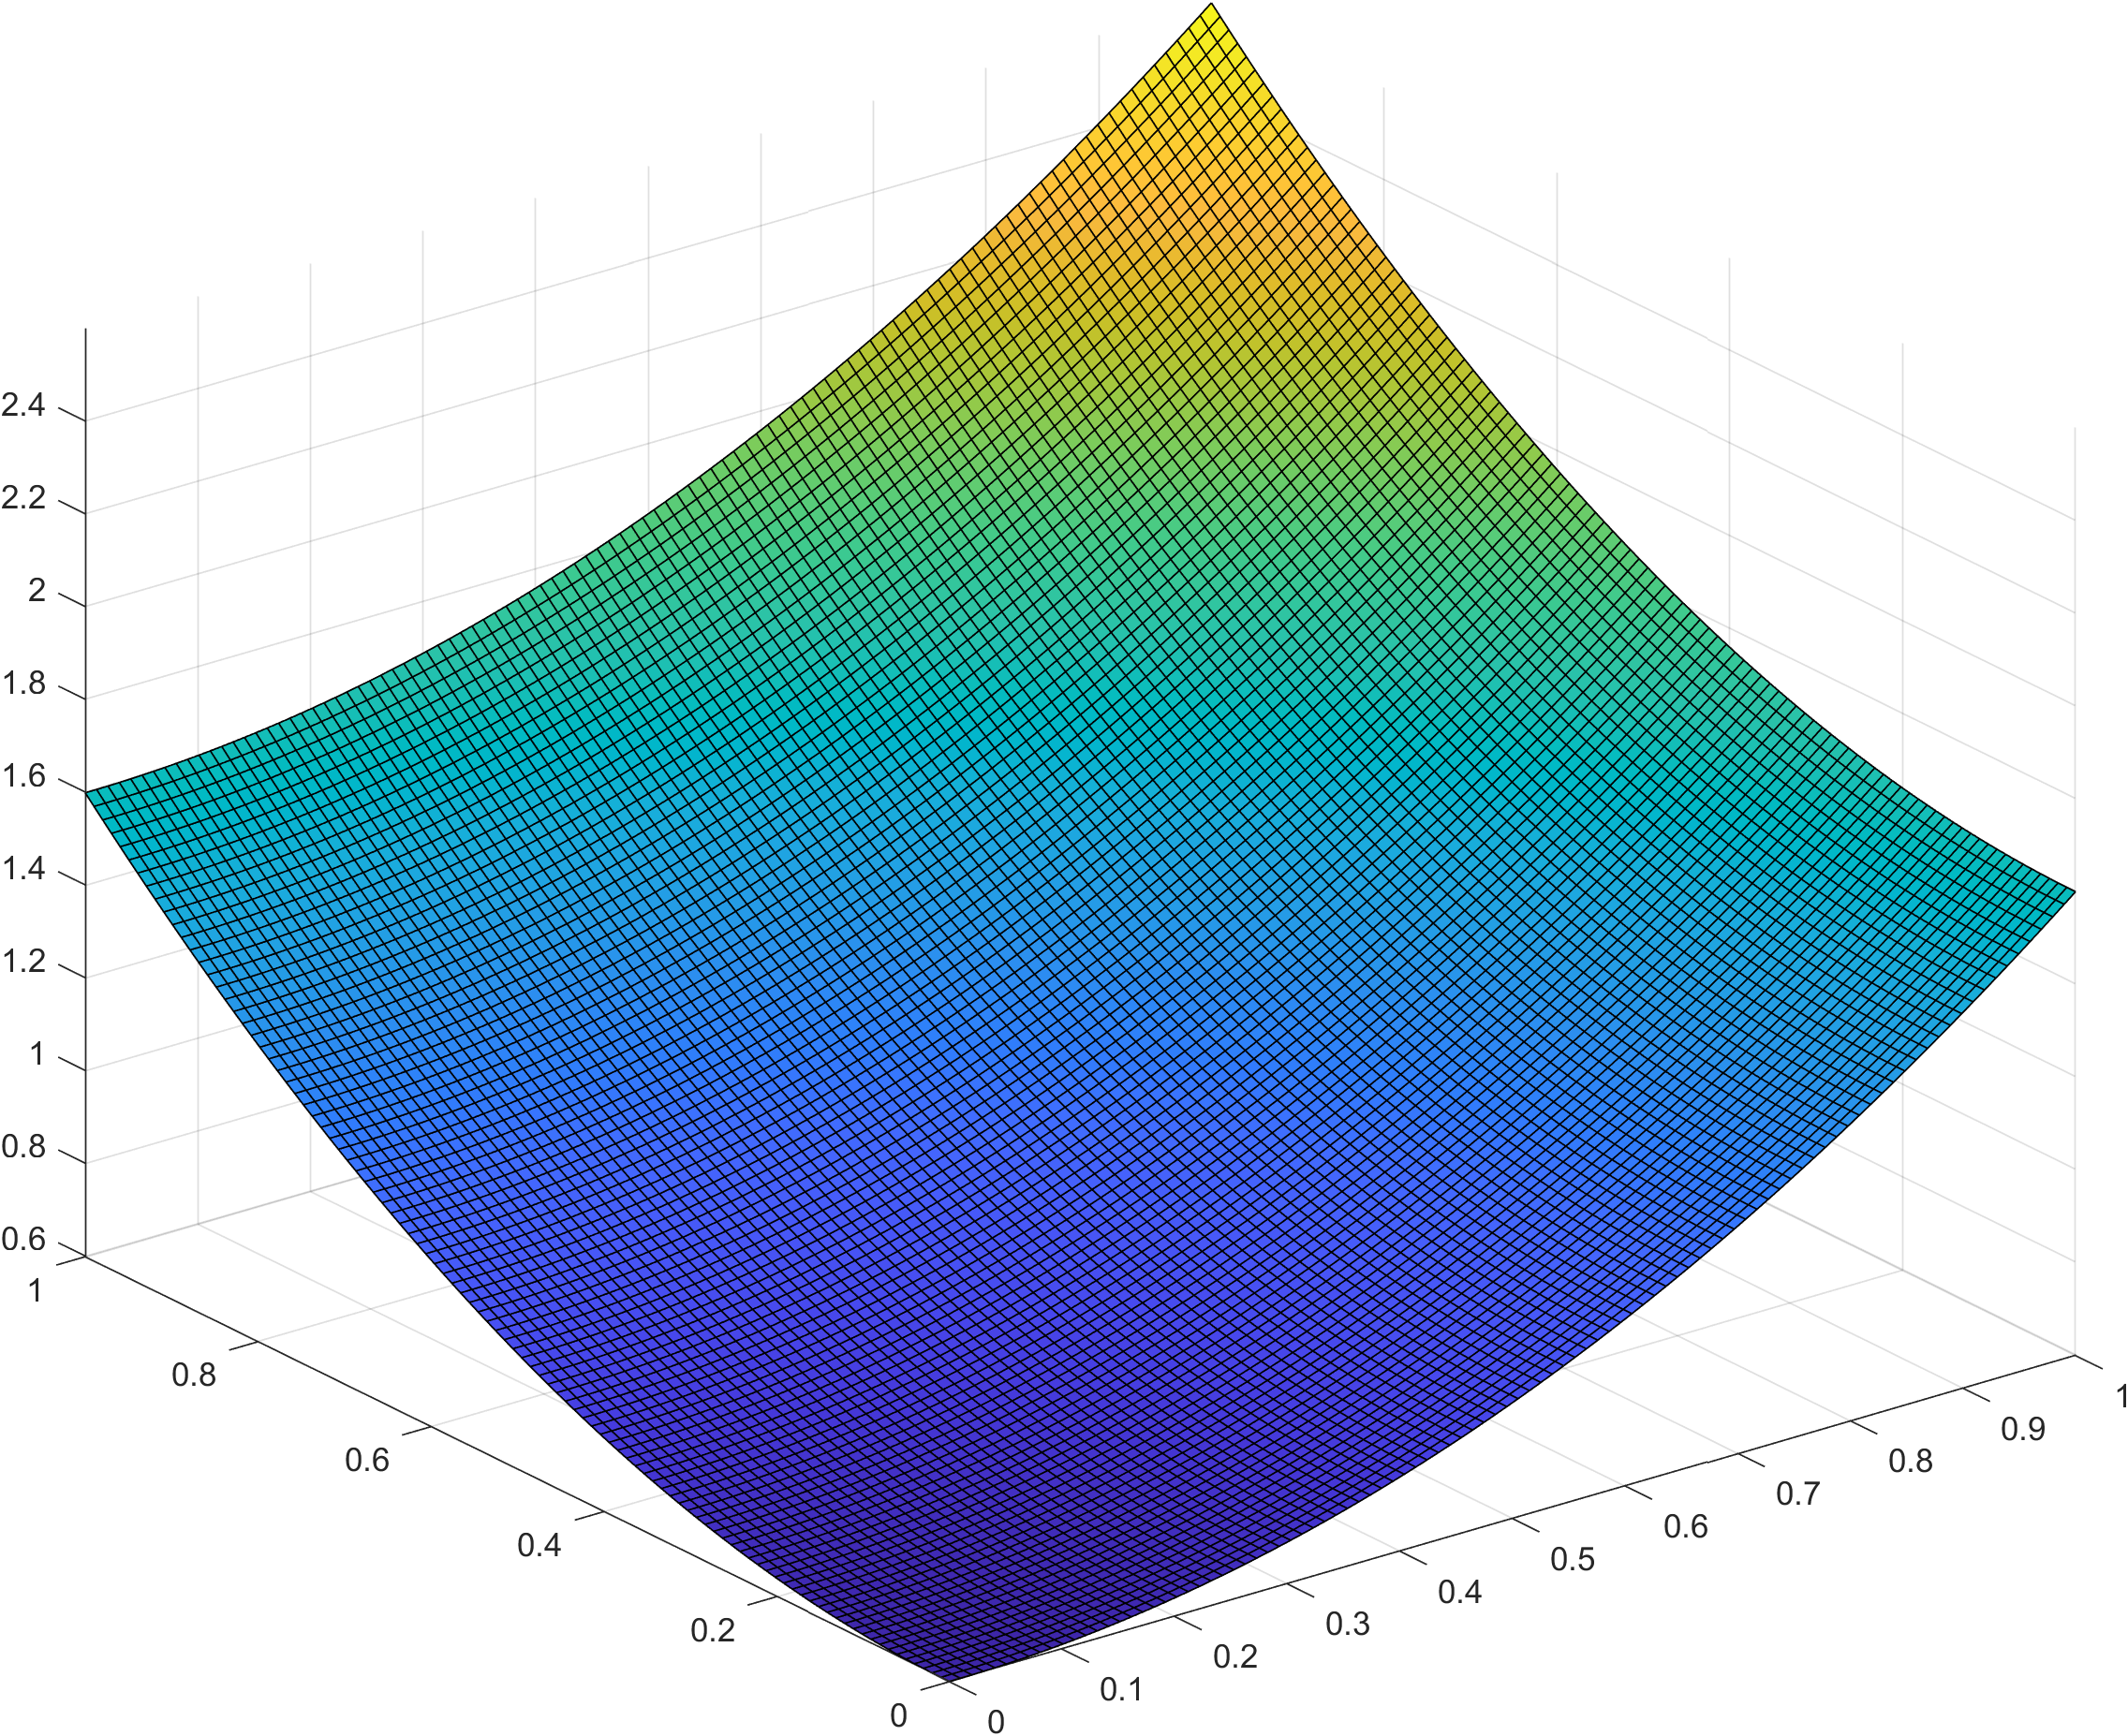
\includegraphics[height=\dimIm]{../Immagini/ET2_SE_NPunti=100_t=0.5.png}
                            \caption{Soluzione esatta al tempo $t=0.5$.}
                            \label{figET2TriangolazioniEsattaTM}
                        \end{subfigure}
                        \begin{subfigure}[t]{\lungSF}
                            \centering
                            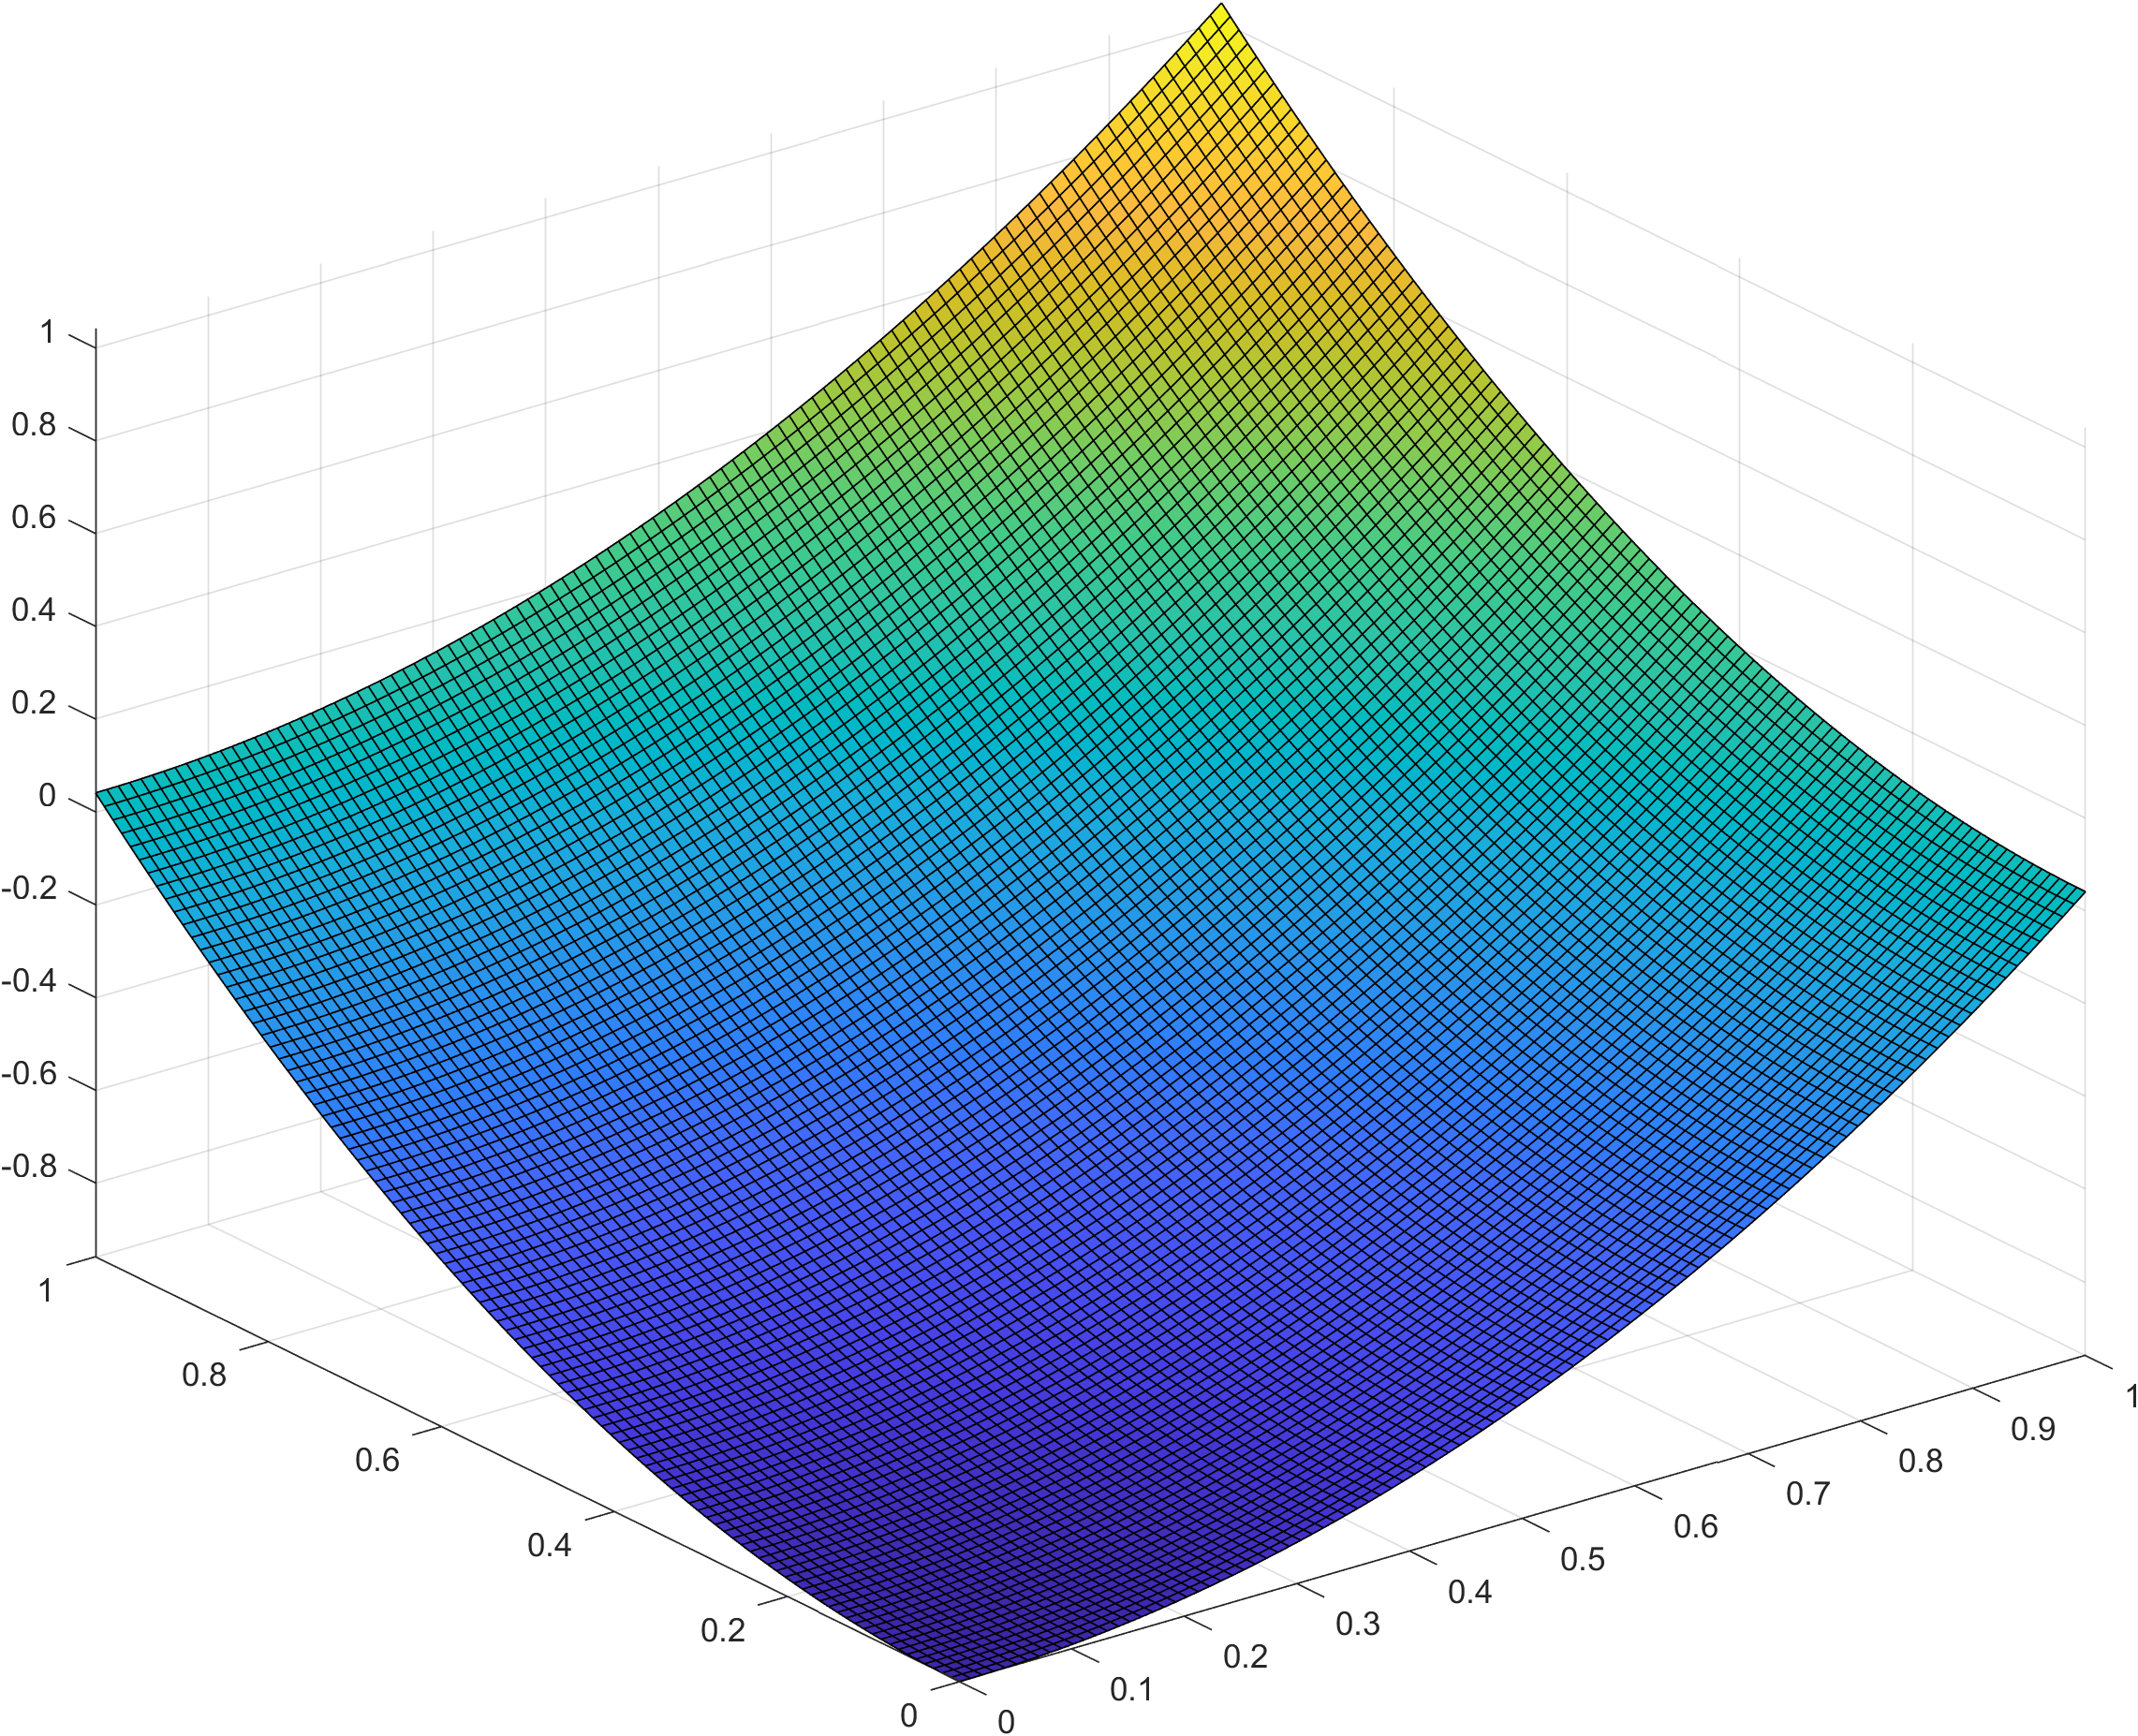
\includegraphics[height=\dimIm]{../Immagini/ET2_SE_NPunti=100_t=1.png}
                            \caption{Soluzione esatta al tempo $t=1$.}
                            \label{figET2TriangolazioniEsattaTF}
                        \end{subfigure}
                    }
                    \distR
                    
                    % \renewcommand{\dimIm}{4cm}
                    \makebox[\linewidth][c]{
                        \captionsetup[subfigure]{width=2.9cm}
                        \SpaziaturaMate{1}{1}{1}
                        \begin{subfigure}[t]{\lungSF}
                            \centering
                            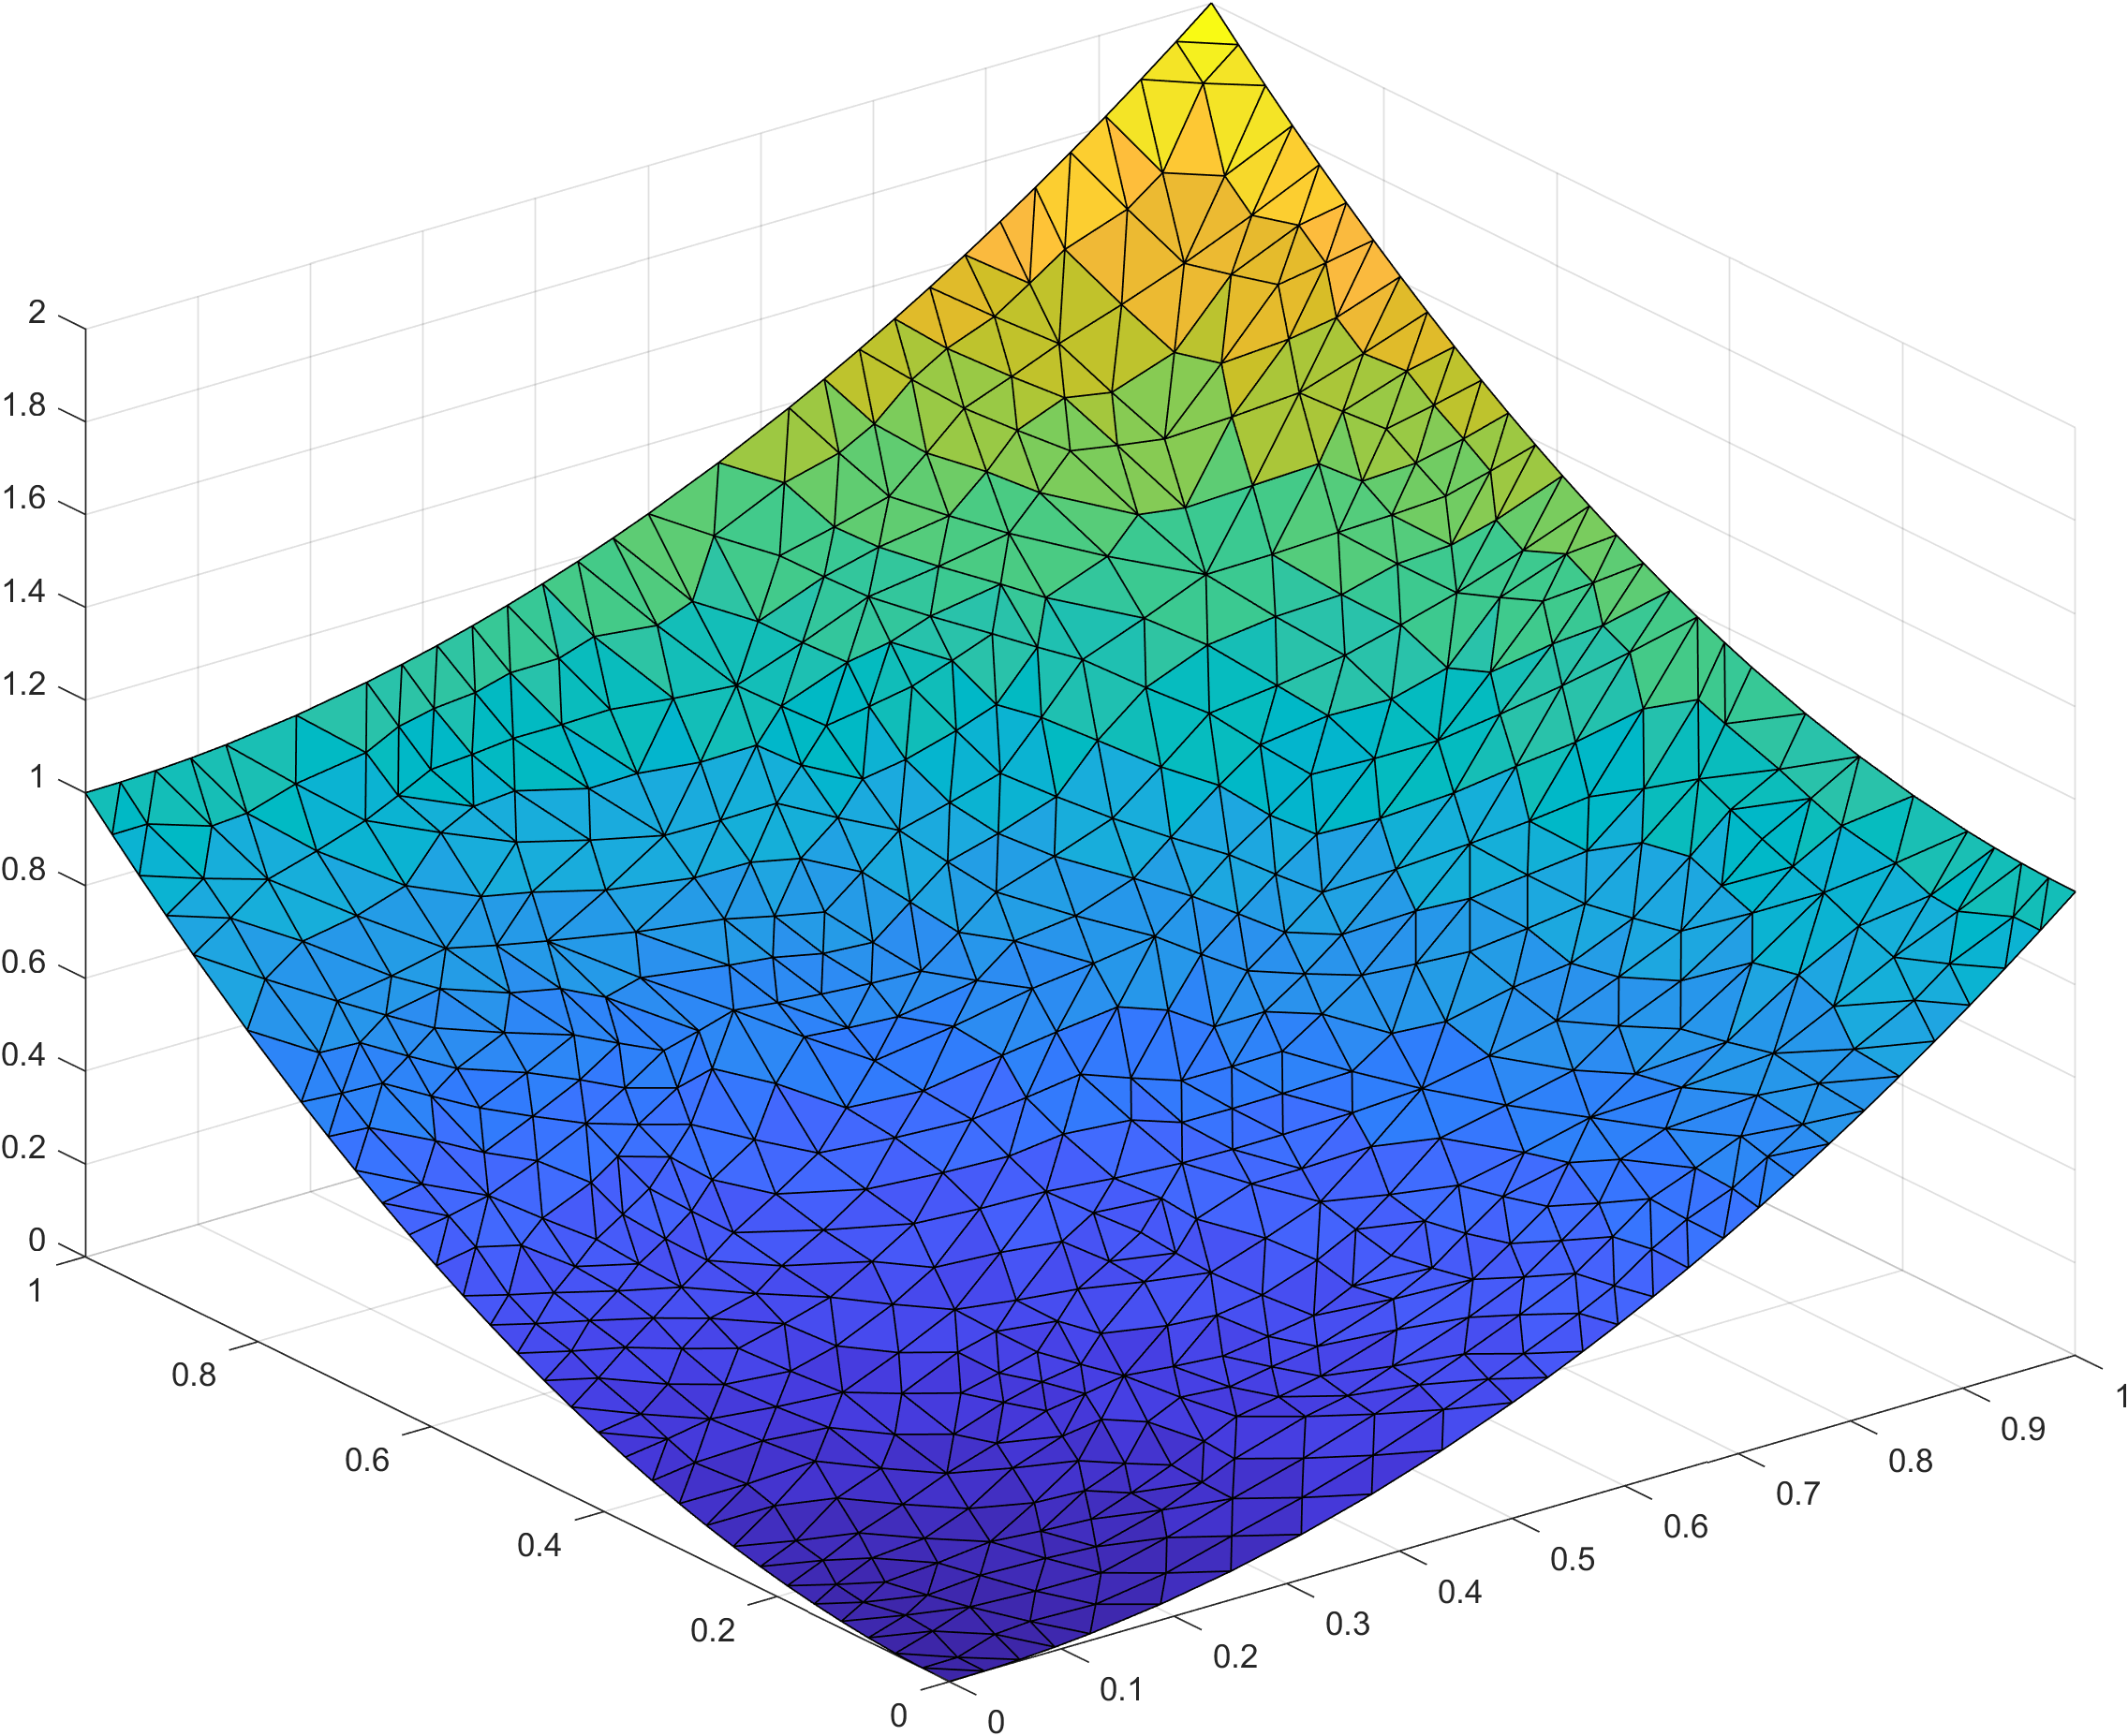
\includegraphics[height=\dimIm]{../Immagini/ET2_P2_AMax=dt=0.005_t=0.png}
                            \caption{Soluzione qualitativa coi $\mathbb{P}_2$ al tempo $t=0$.}
                            \label{figET2TriangolazioniP2TI}
                        \end{subfigure}
                        \begin{subfigure}[t]{\lungSF}
                            \centering
                            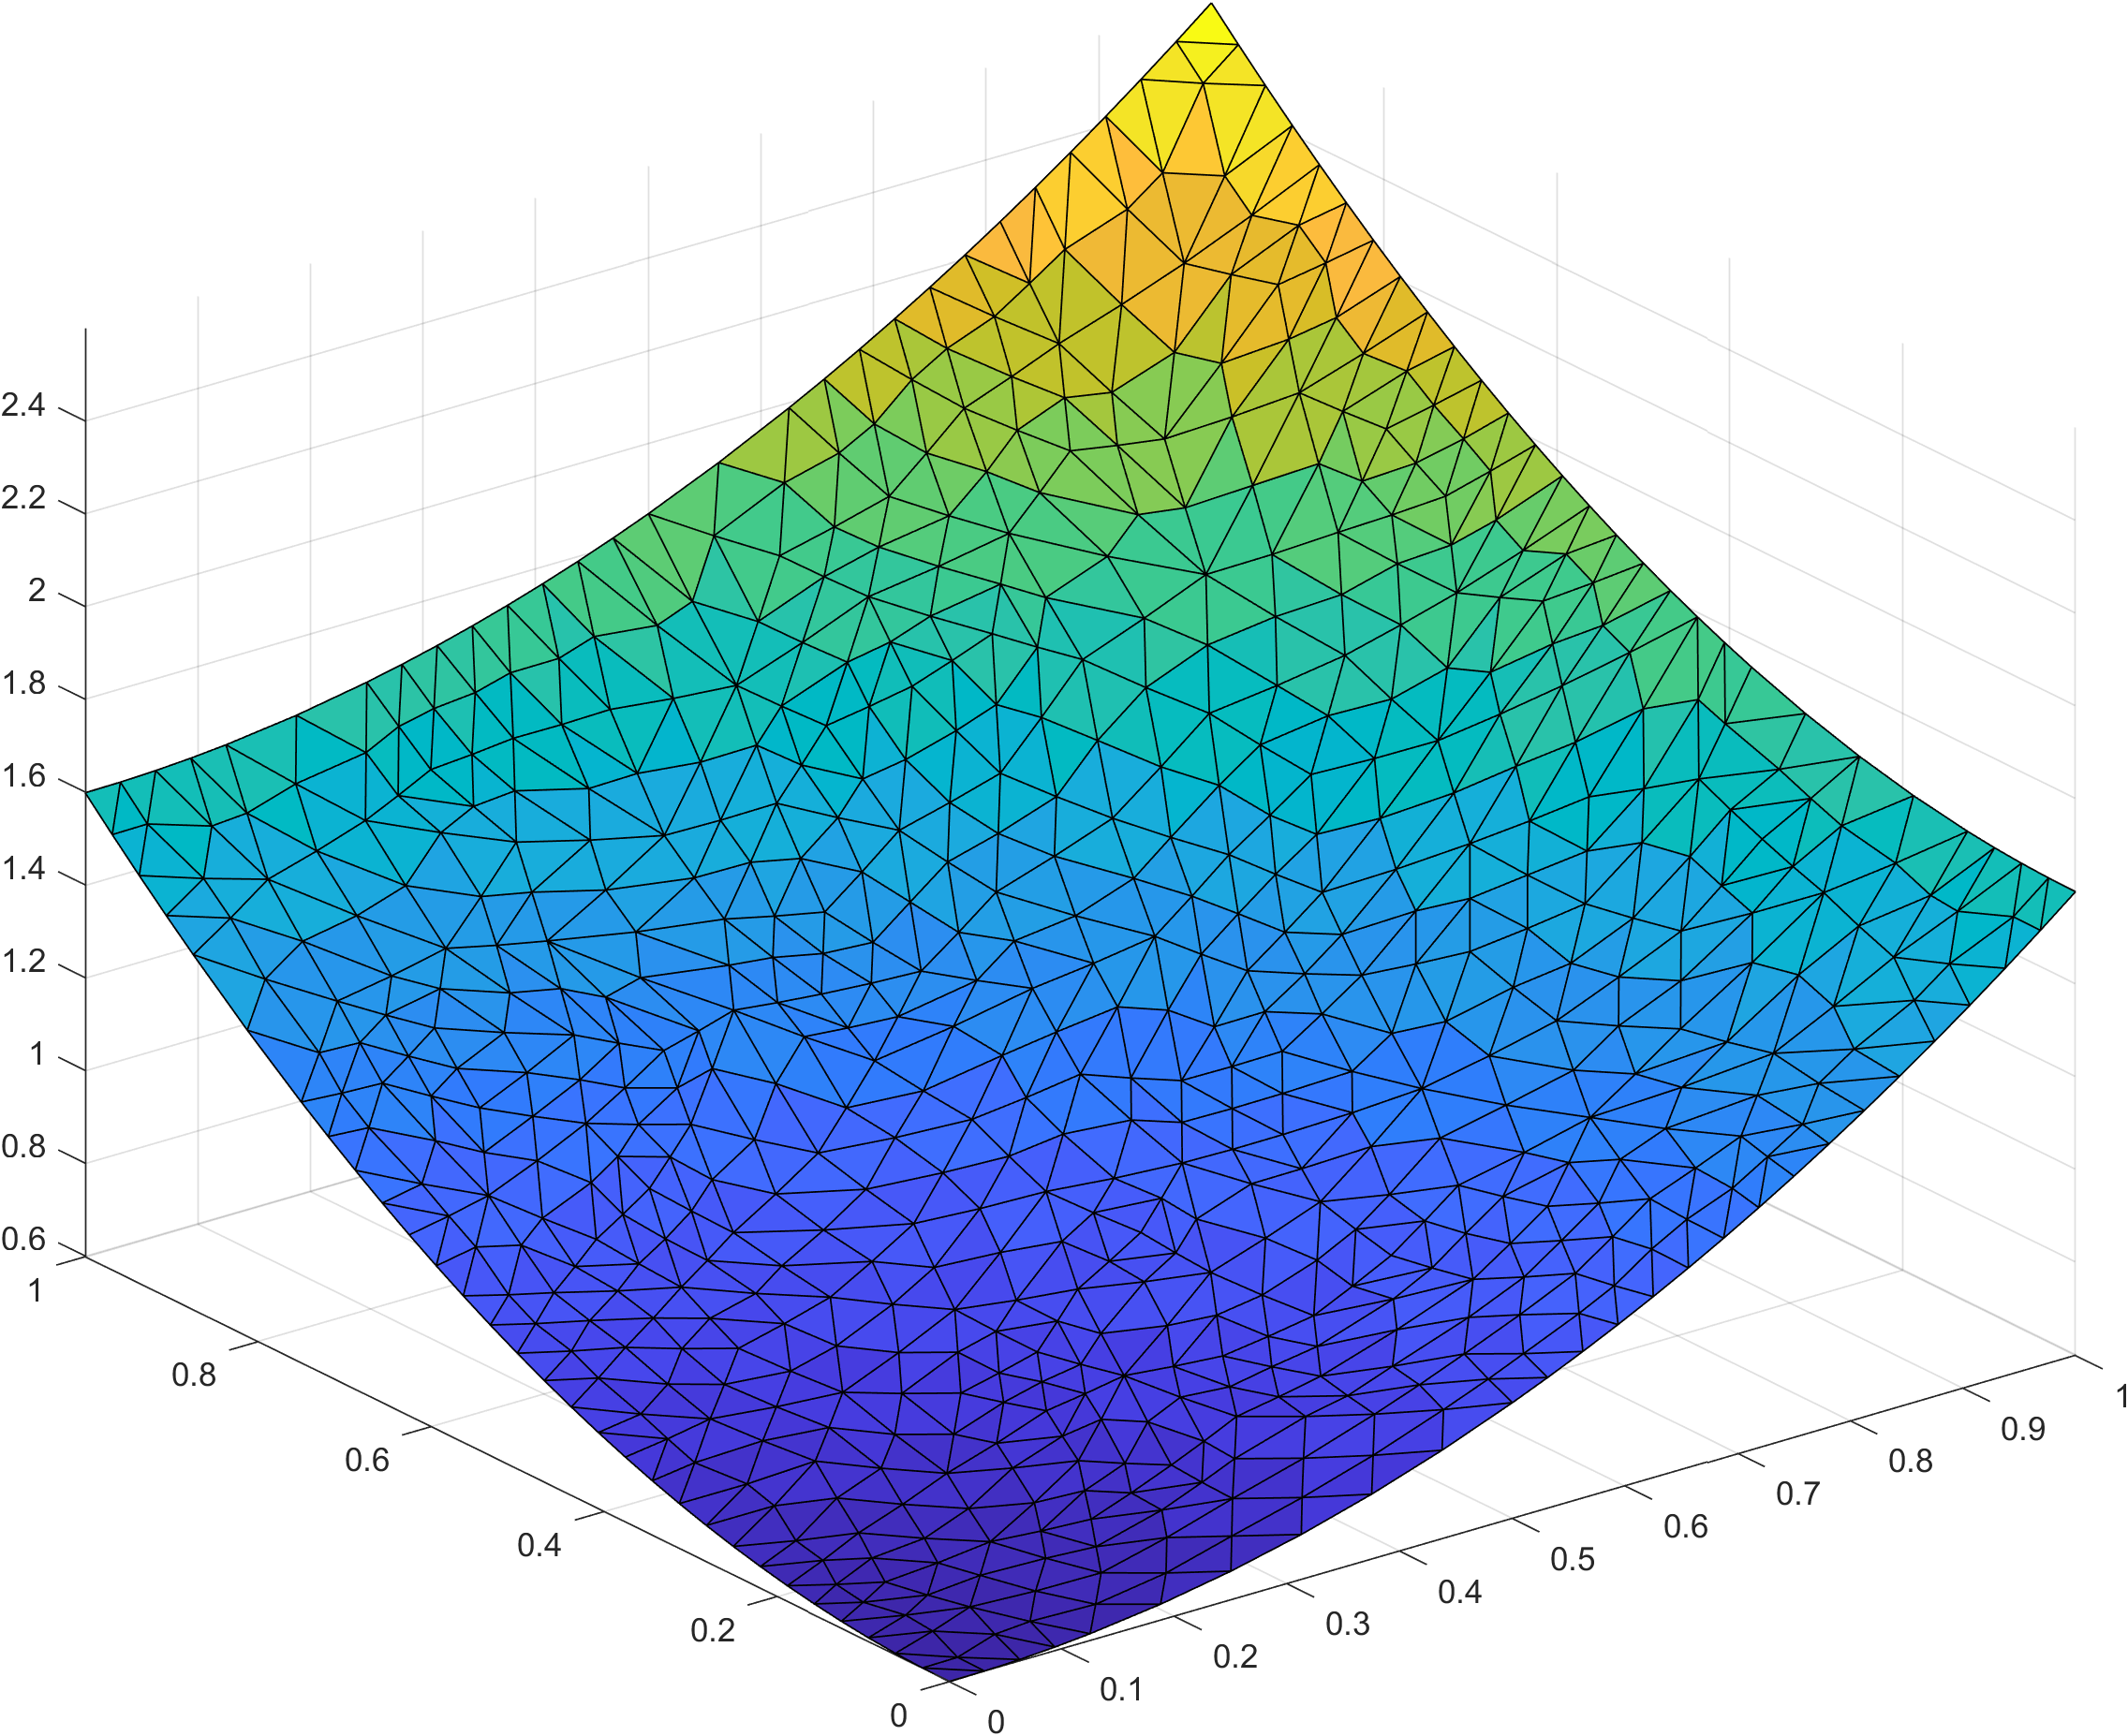
\includegraphics[height=\dimIm]{../Immagini/ET2_P2_AMax=dt=0.005_t=0.5.png}
                            \caption{Soluzione qualitativa coi $\mathbb{P}_2$ al tempo $t=0.5$.}
                            \label{figET2TriangolazioniP2TM}
                        \end{subfigure}
                        \begin{subfigure}[t]{\lungSF}
                            \centering
                            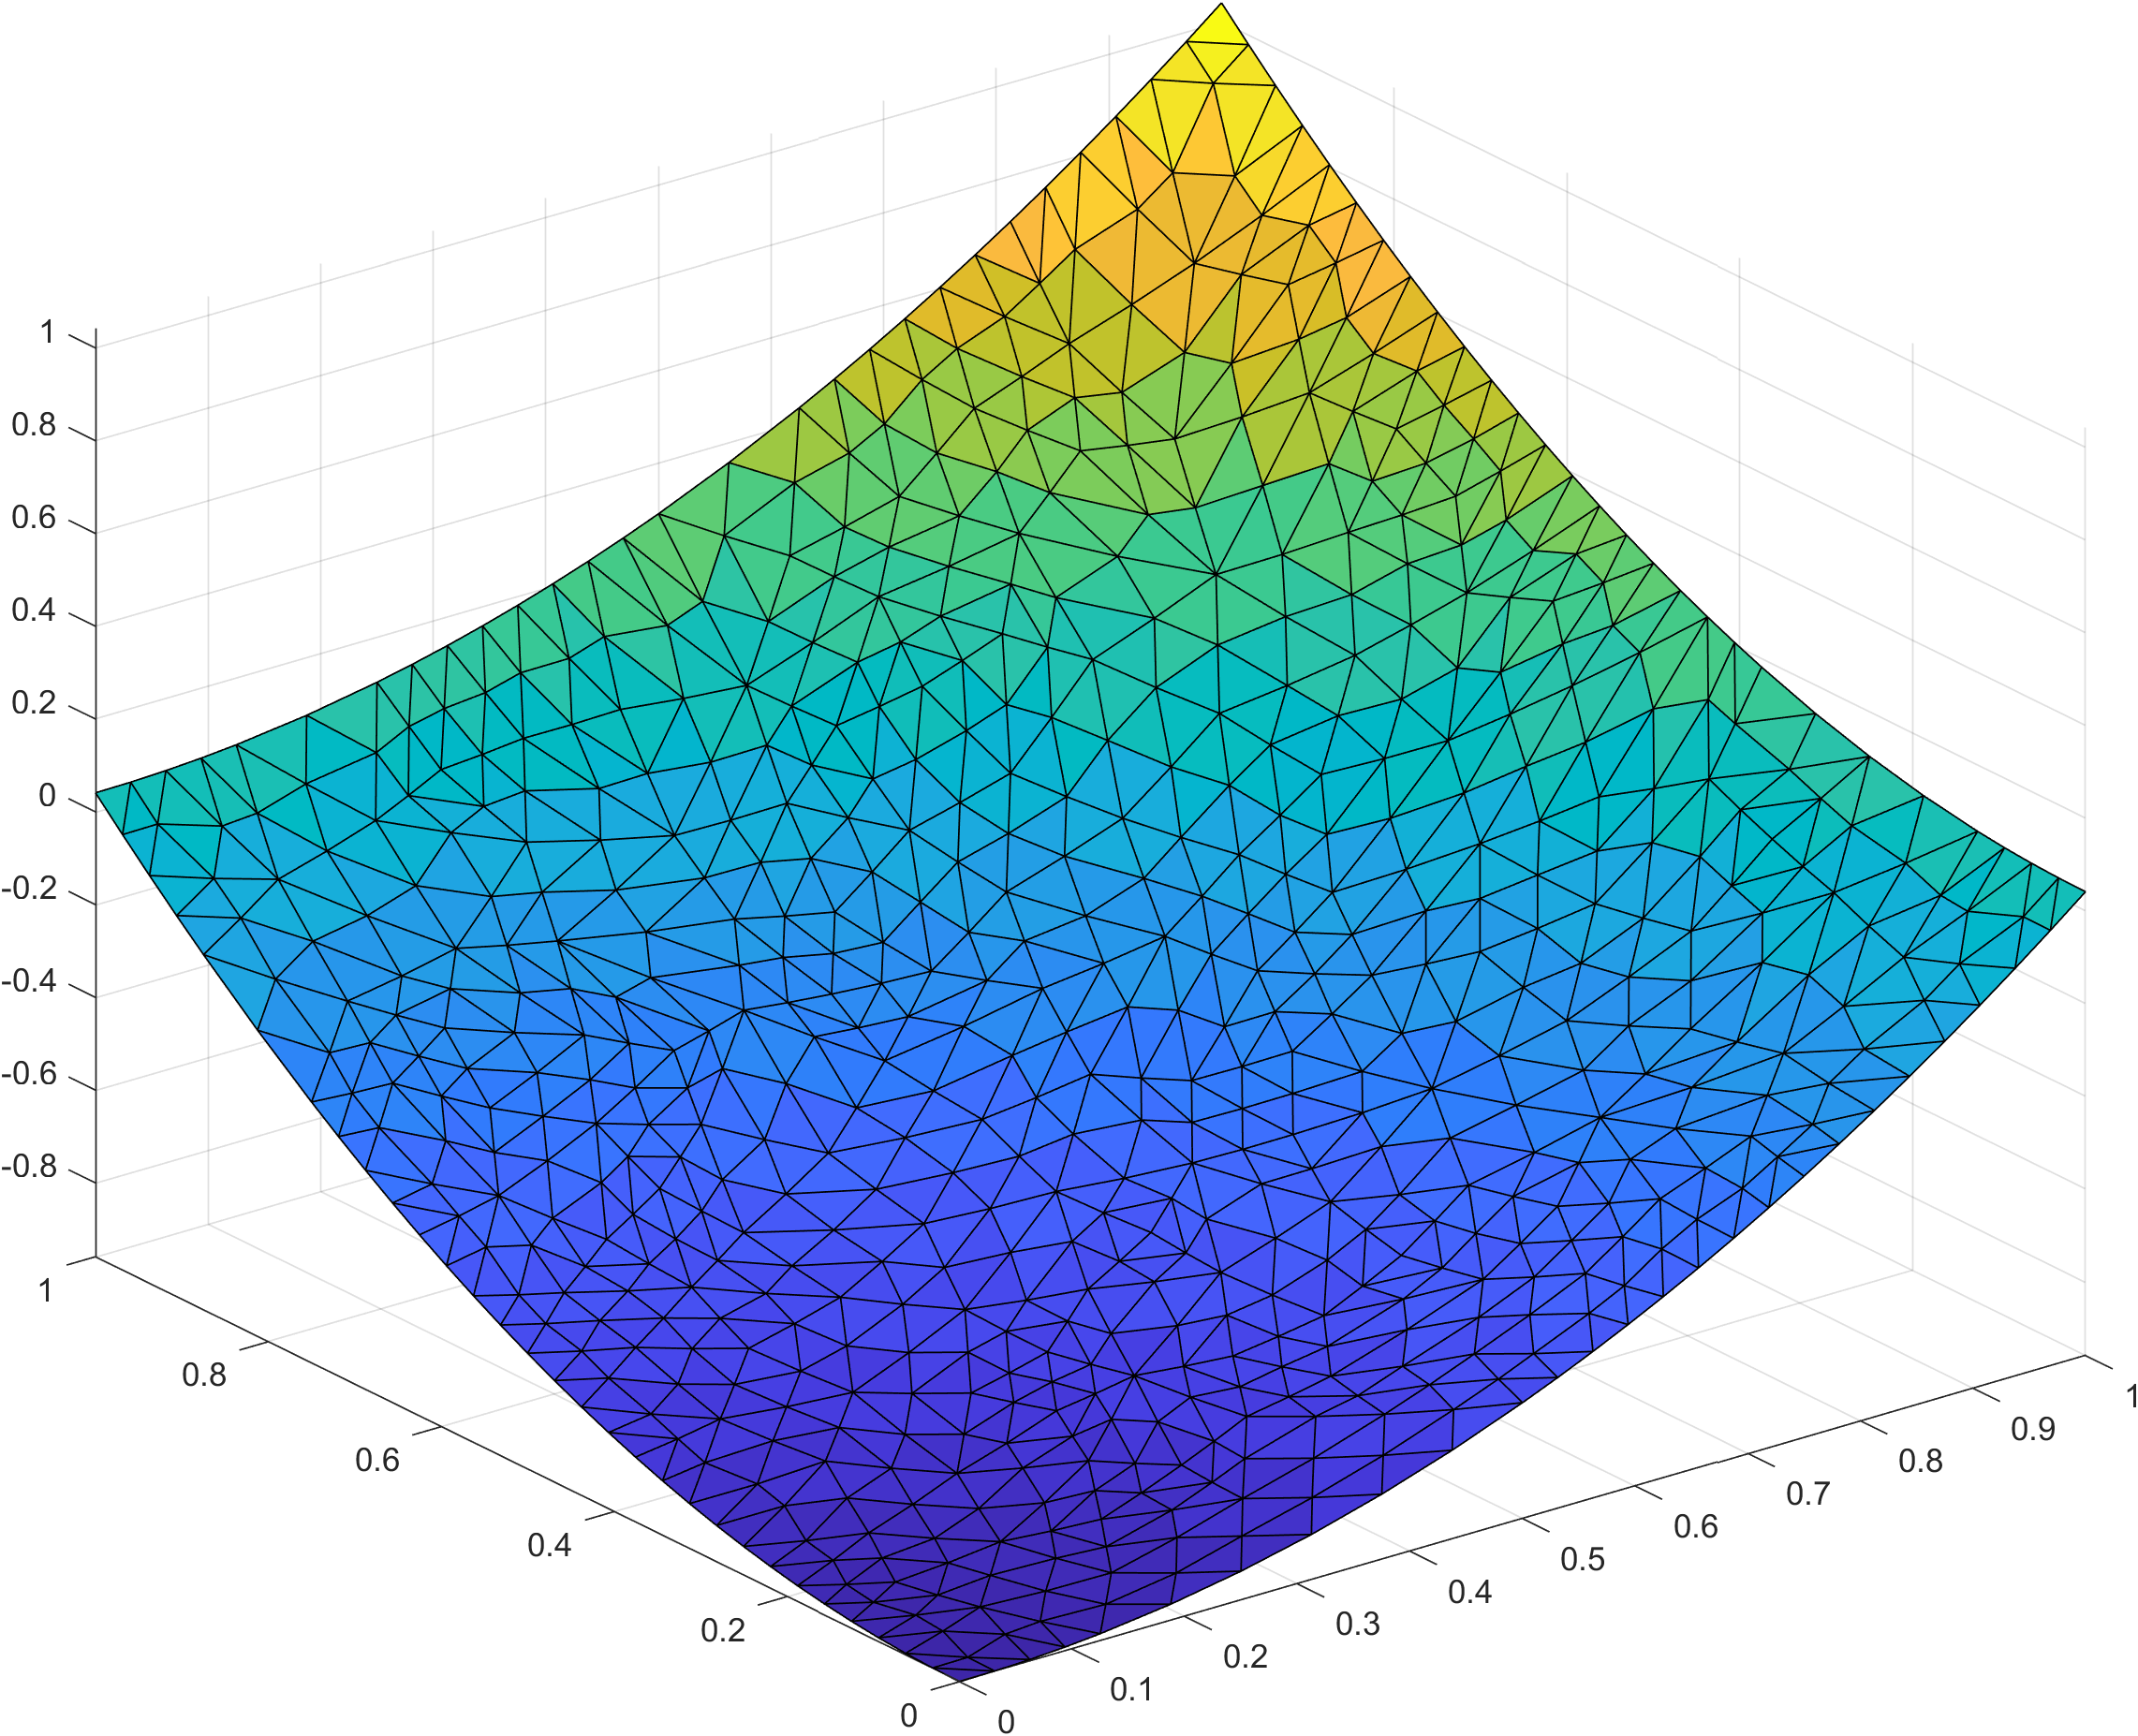
\includegraphics[height=\dimIm]{../Immagini/ET2_P2_AMax=dt=0.005_t=1.png}
                            \caption{Soluzione qualitativa coi $\mathbb{P}_2$ al tempo $t=1$.}
                            \label{figET2TriangolazioniP2TF}
                        \end{subfigure}
                    }
                    \distR
        
                    \renewcommand{\lungSF}{.5\linewidth}
                    \renewcommand{\dimIm}{\linewidth}
                    \newcommand{\distC}{\hspace{7.5pt}} % Distanza tra le colonne
                    \makebox[\linewidth][c]{
                        \begin{subfigure}[c]{\lungSF}
                            \centering
                            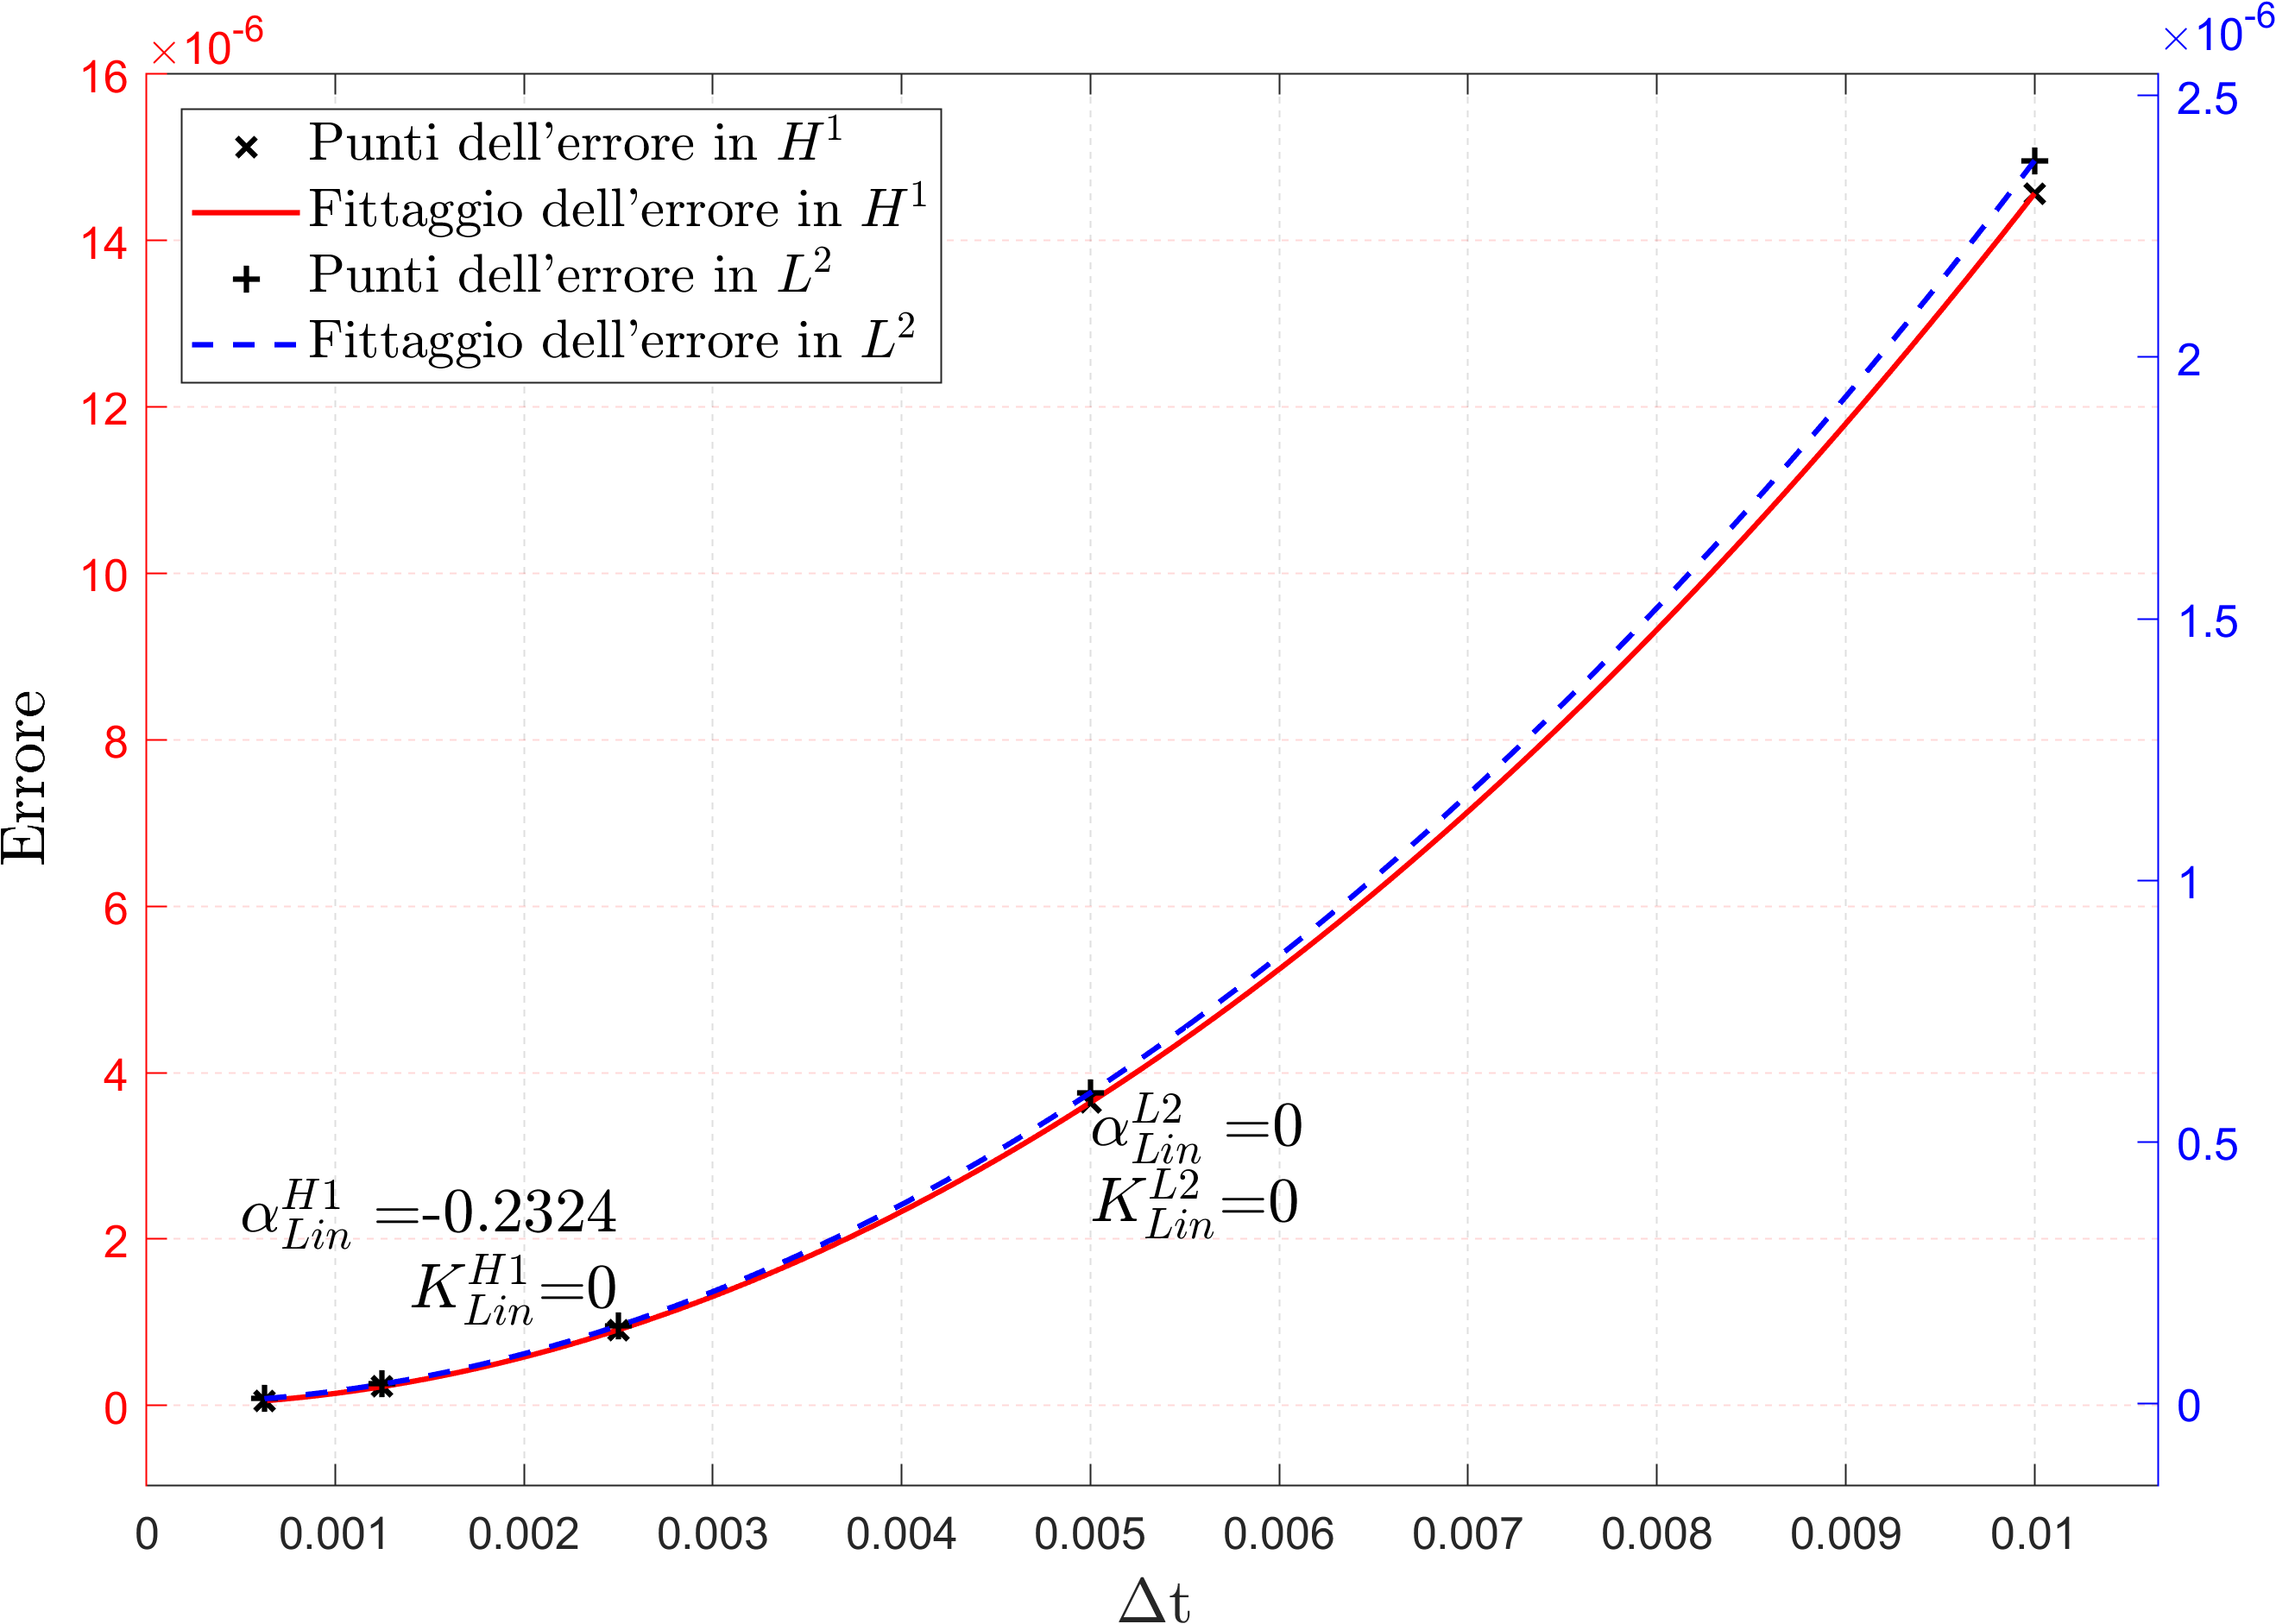
\includegraphics[width=\dimIm]{../Immagini/ET2_P2_ErrLin_AMax=dt=0.01_NSim=5.png}
                        \caption{Errore dei $\mathbb{P}_2$ in scala lineare.}
                        \label{figET2ErroreP2Lin}
                        \end{subfigure}
                        \distC
                        \begin{subfigure}[c]{\lungSF}
                            \centering
                            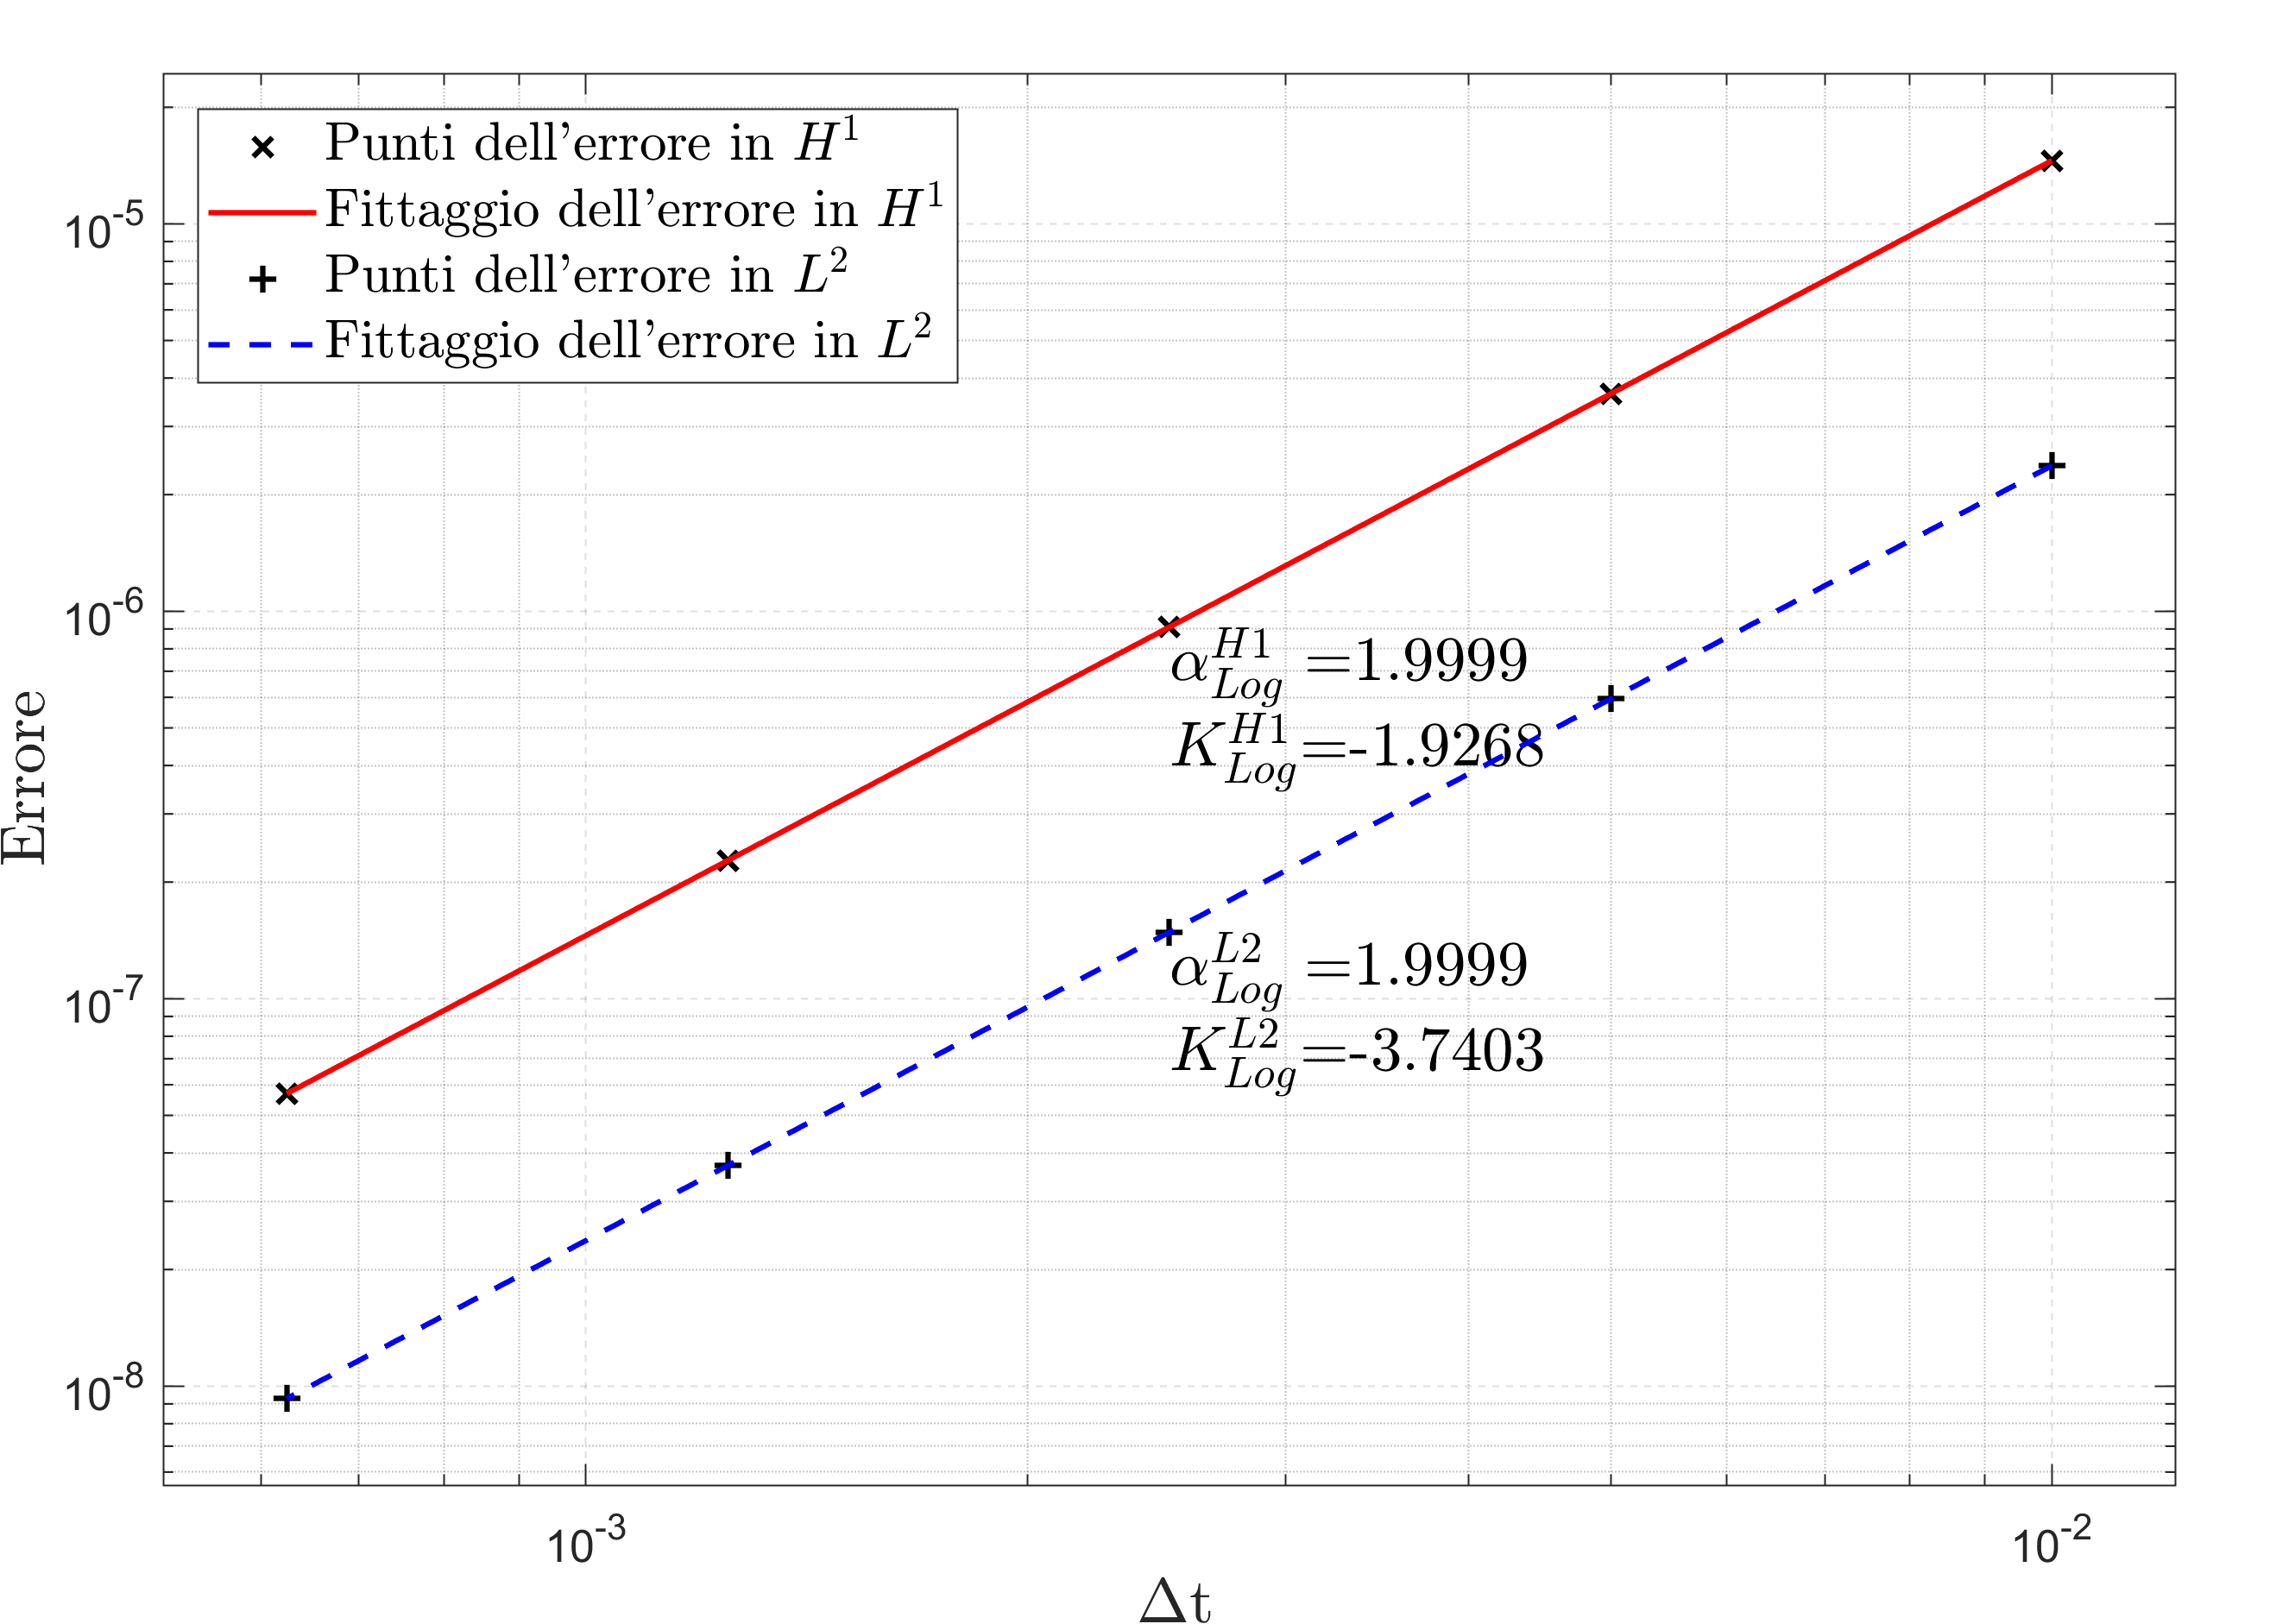
\includegraphics[width=\dimIm]{../Immagini/ET2_P2_ErrLog_AMax=dt=0.01_NSim=5.png}
                        \caption{Errore dei $\mathbb{P}_2$ in scala logaritmica.}
                        \label{figET2ErroreP2Log}
                        \end{subfigure}
                    }
                    \caption{Nelle Figg. \ref{figET2TriangolazioniEsattaTI}-\ref{figET2TriangolazioniP2TF} sono mostrate le soluzioni dell'ET2 in tre istanti temporali: le prime tre mostrano la soluzione esatta e le restanti quella approssimata; invece nelle \ref{figET2ErroreP2Lin} e \ref{figET2ErroreP2Log} sono illustrati in due scale diverse gli errori in norma $H^1$ ed $L^2$. I parametri dati a \textit{BBTR} sono spiegati nel $\S$\ref{parPremessaParametriBBTR}.}
                    \label{figET2}
                \end{figure*}
                %%%%%%%%%%%%%%%%%%
                %%%%%%%%%%%%%%%%%%
                %%%%%%%%%%%%%%%%%%

                %%%%%%%%%%%%%%%%%%%%%%
                %%% Infopagina ES1 %%%
                %%%%%%%%%%%%%%%%%%%%%%
                \begin{figure*}[p]
                    \newcommand{\distR}{\vspace{15pt}} % Distanza tra le righe
                    
                    \newcommand{\lungSF}{0.33\textwidth}
                    \newcommand{\dimIm}{4.6cm}
                    \makebox[\linewidth][c]{
                        % \captionsetup[subfigure]{width=2.4cm}
                        \SpaziaturaMate{1}{1}{1}
                        \begin{subfigure}[t]{\lungSF}
                            \centering
                            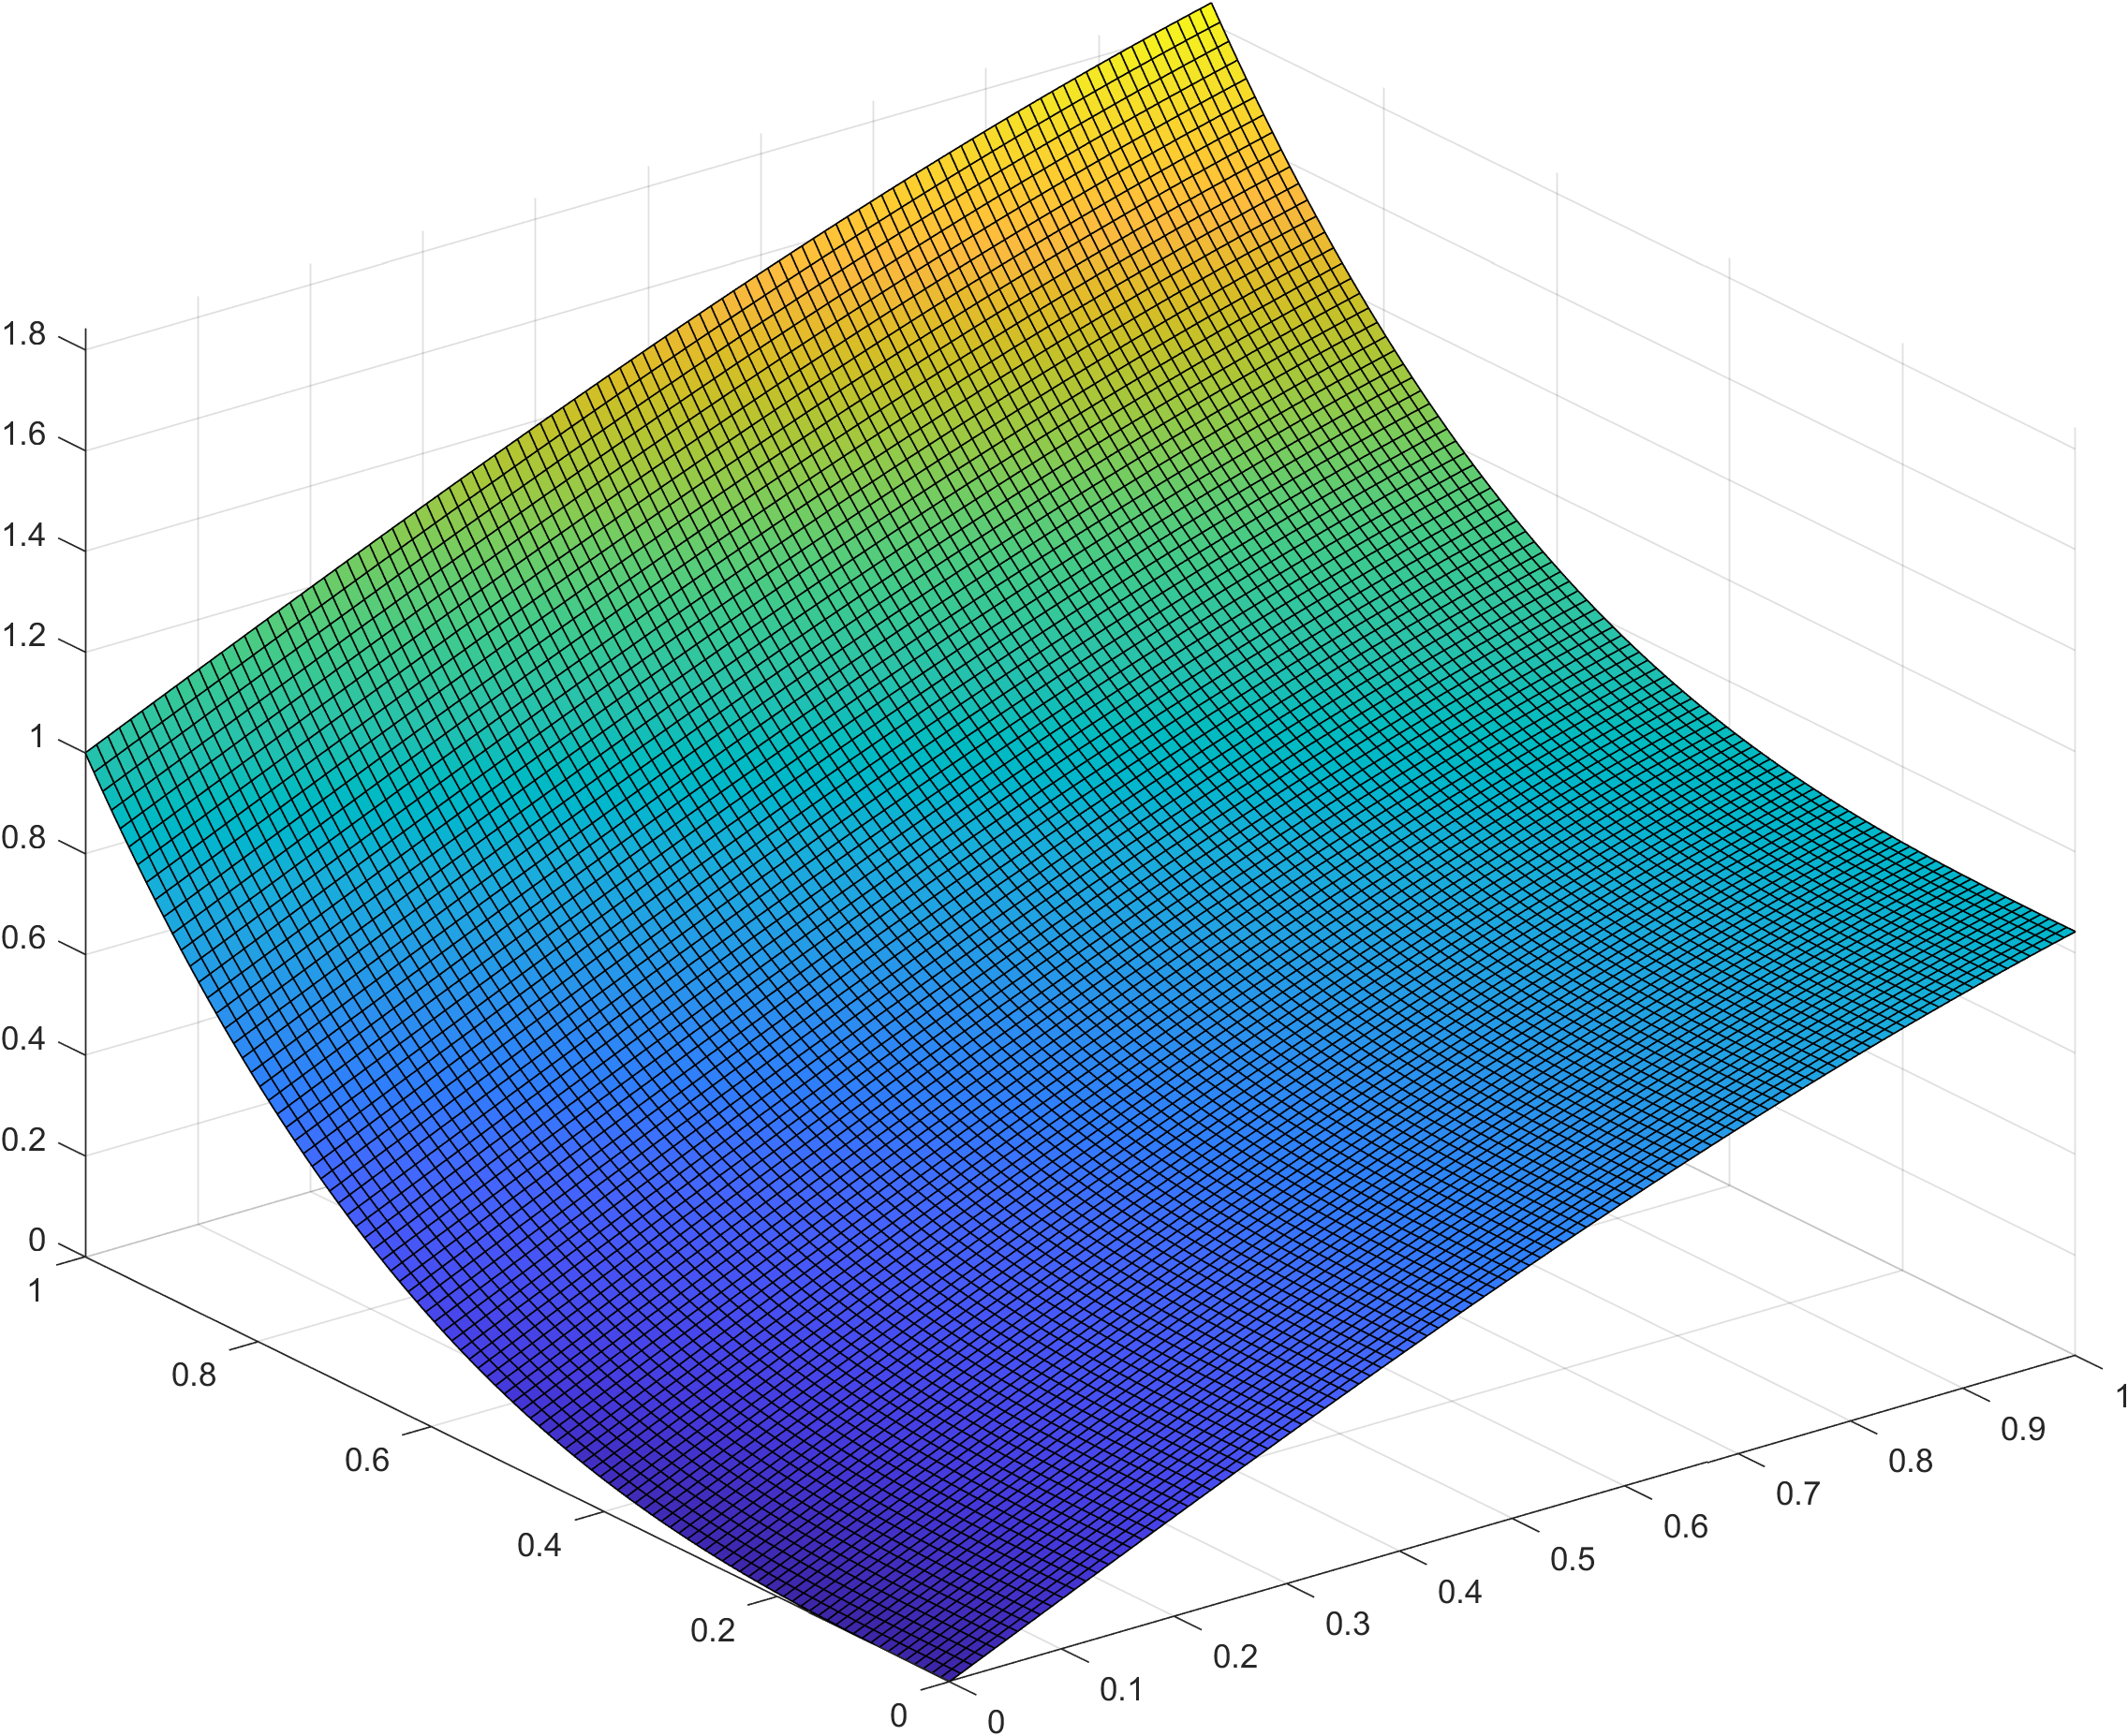
\includegraphics[height=\dimIm]{../Immagini/ES12_SE_NPunti=100_t=0.png}
                            \caption{Soluzione esatta al tempo $t=0$.}
                            \label{figES1TriangolazioniEsattaTI}
                        \end{subfigure}
                        \begin{subfigure}[t]{\lungSF}
                            \centering
                            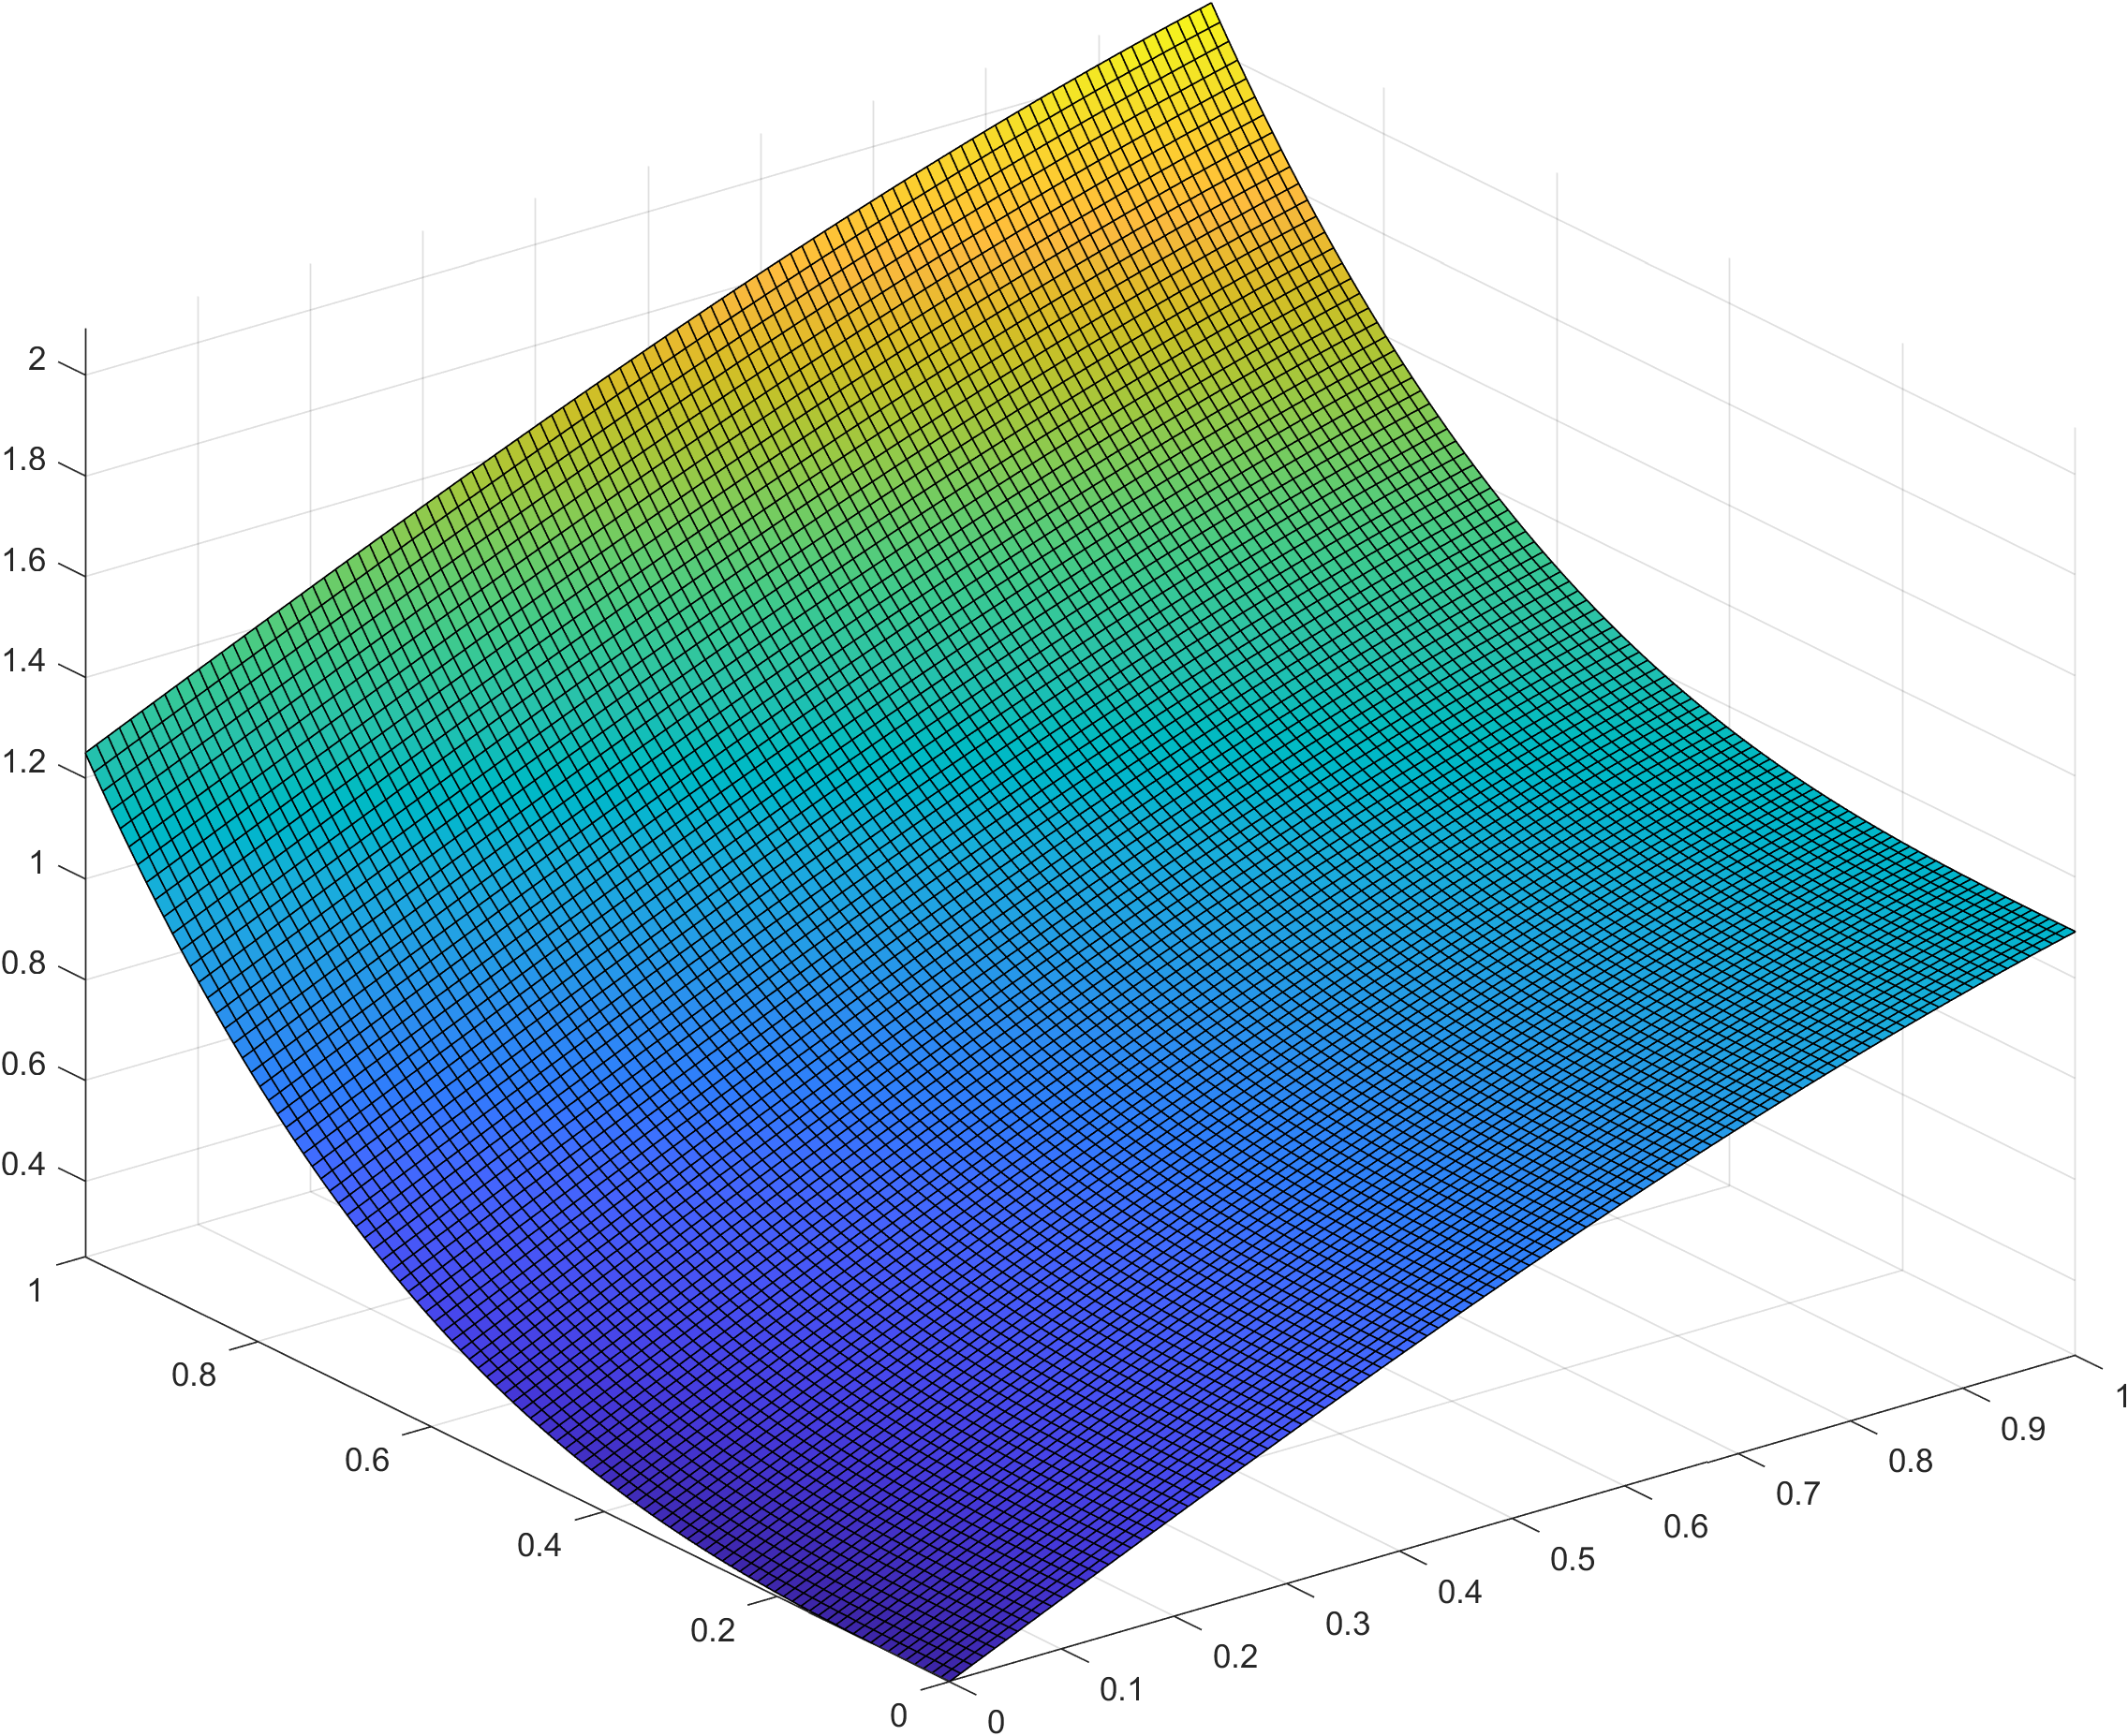
\includegraphics[height=\dimIm]{../Immagini/ES12_SE_NPunti=100_t=0.5.png}
                            \caption{Soluzione esatta al tempo $t=0.5$.}
                            \label{figES1TriangolazioniEsattaTM}
                        \end{subfigure}
                        \begin{subfigure}[t]{\lungSF}
                            \centering
                            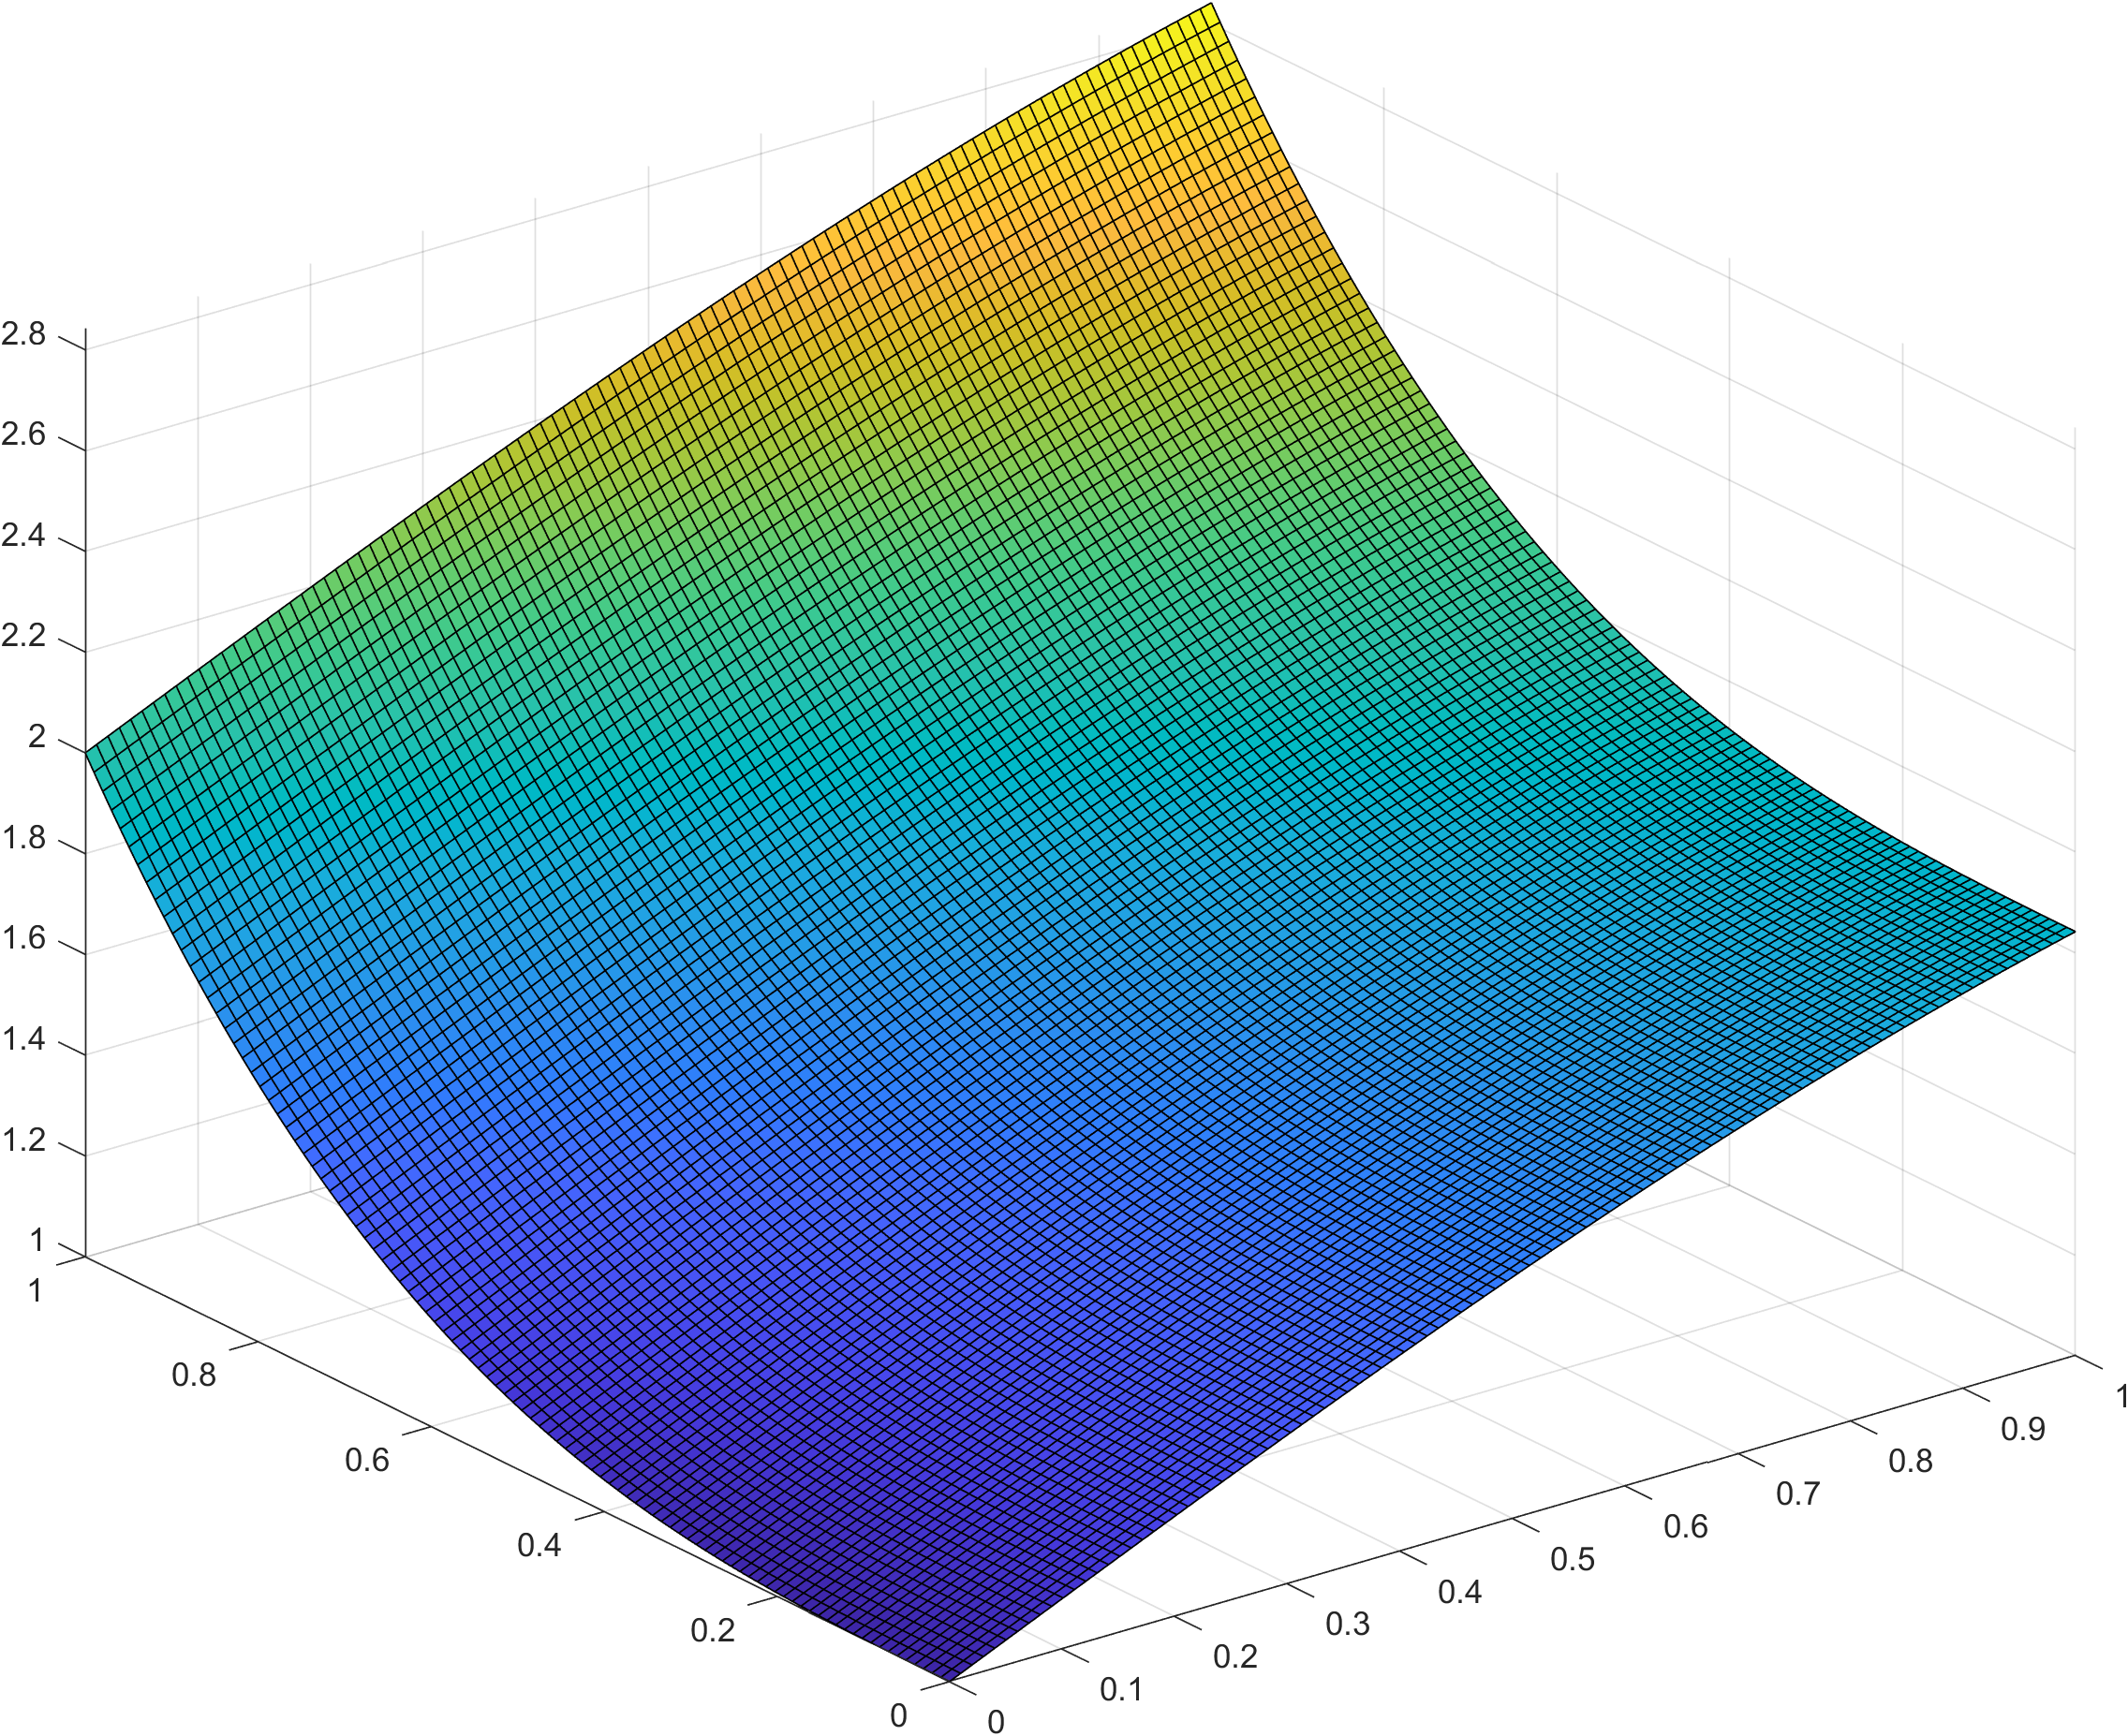
\includegraphics[height=\dimIm]{../Immagini/ES12_SE_NPunti=100_t=1.png}
                            \caption{Soluzione esatta al tempo $t=1$.}
                            \label{figES1TriangolazioniEsattaTF}
                        \end{subfigure}
                    }
                    \distR
                    
                    % \renewcommand{\dimIm}{4cm}
                    \makebox[\linewidth][c]{
                        \captionsetup[subfigure]{width=2.9cm}
                        \SpaziaturaMate{1}{1}{1}
                        \begin{subfigure}[t]{\lungSF}
                            \centering
                            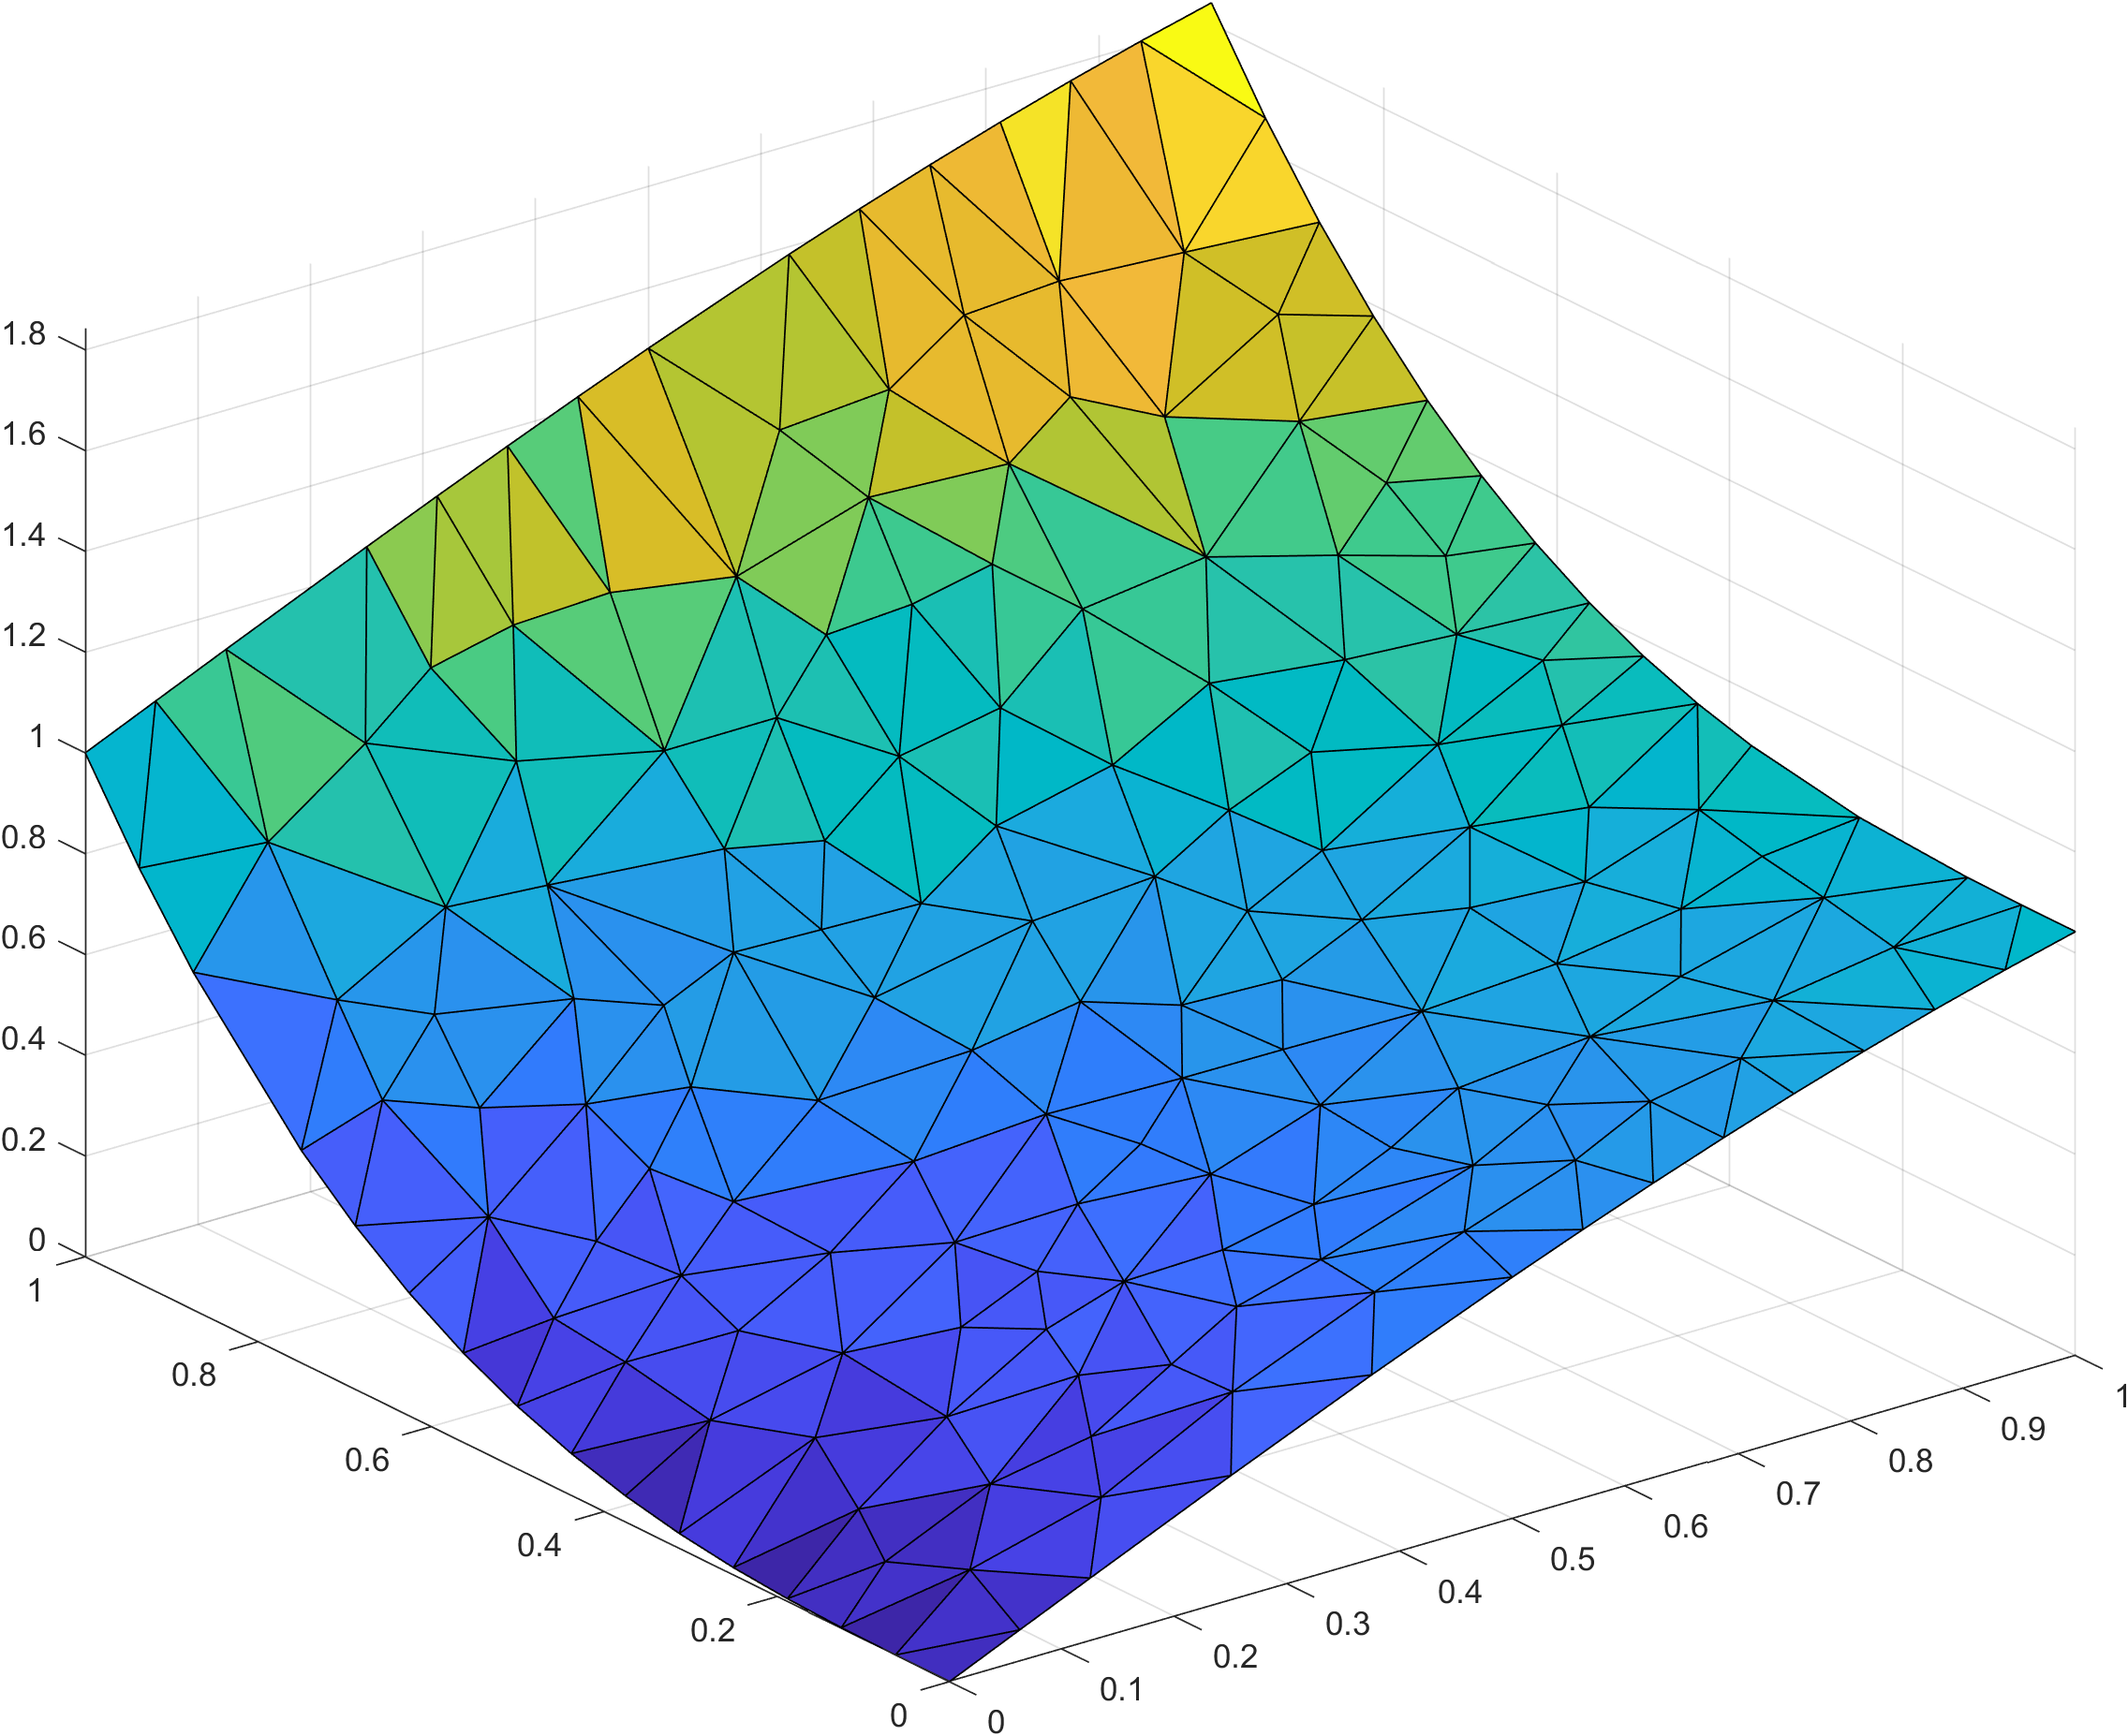
\includegraphics[height=\dimIm]{../Immagini/ES1_P1_AMax=dt=0.005_t=0.png}
                            \caption{Soluzione qualitativa coi $\mathbb{P}_1$ al tempo $t=0$.}
                            \label{figES1TriangolazioniP1TI}
                        \end{subfigure}
                        \begin{subfigure}[t]{\lungSF}
                            \centering
                            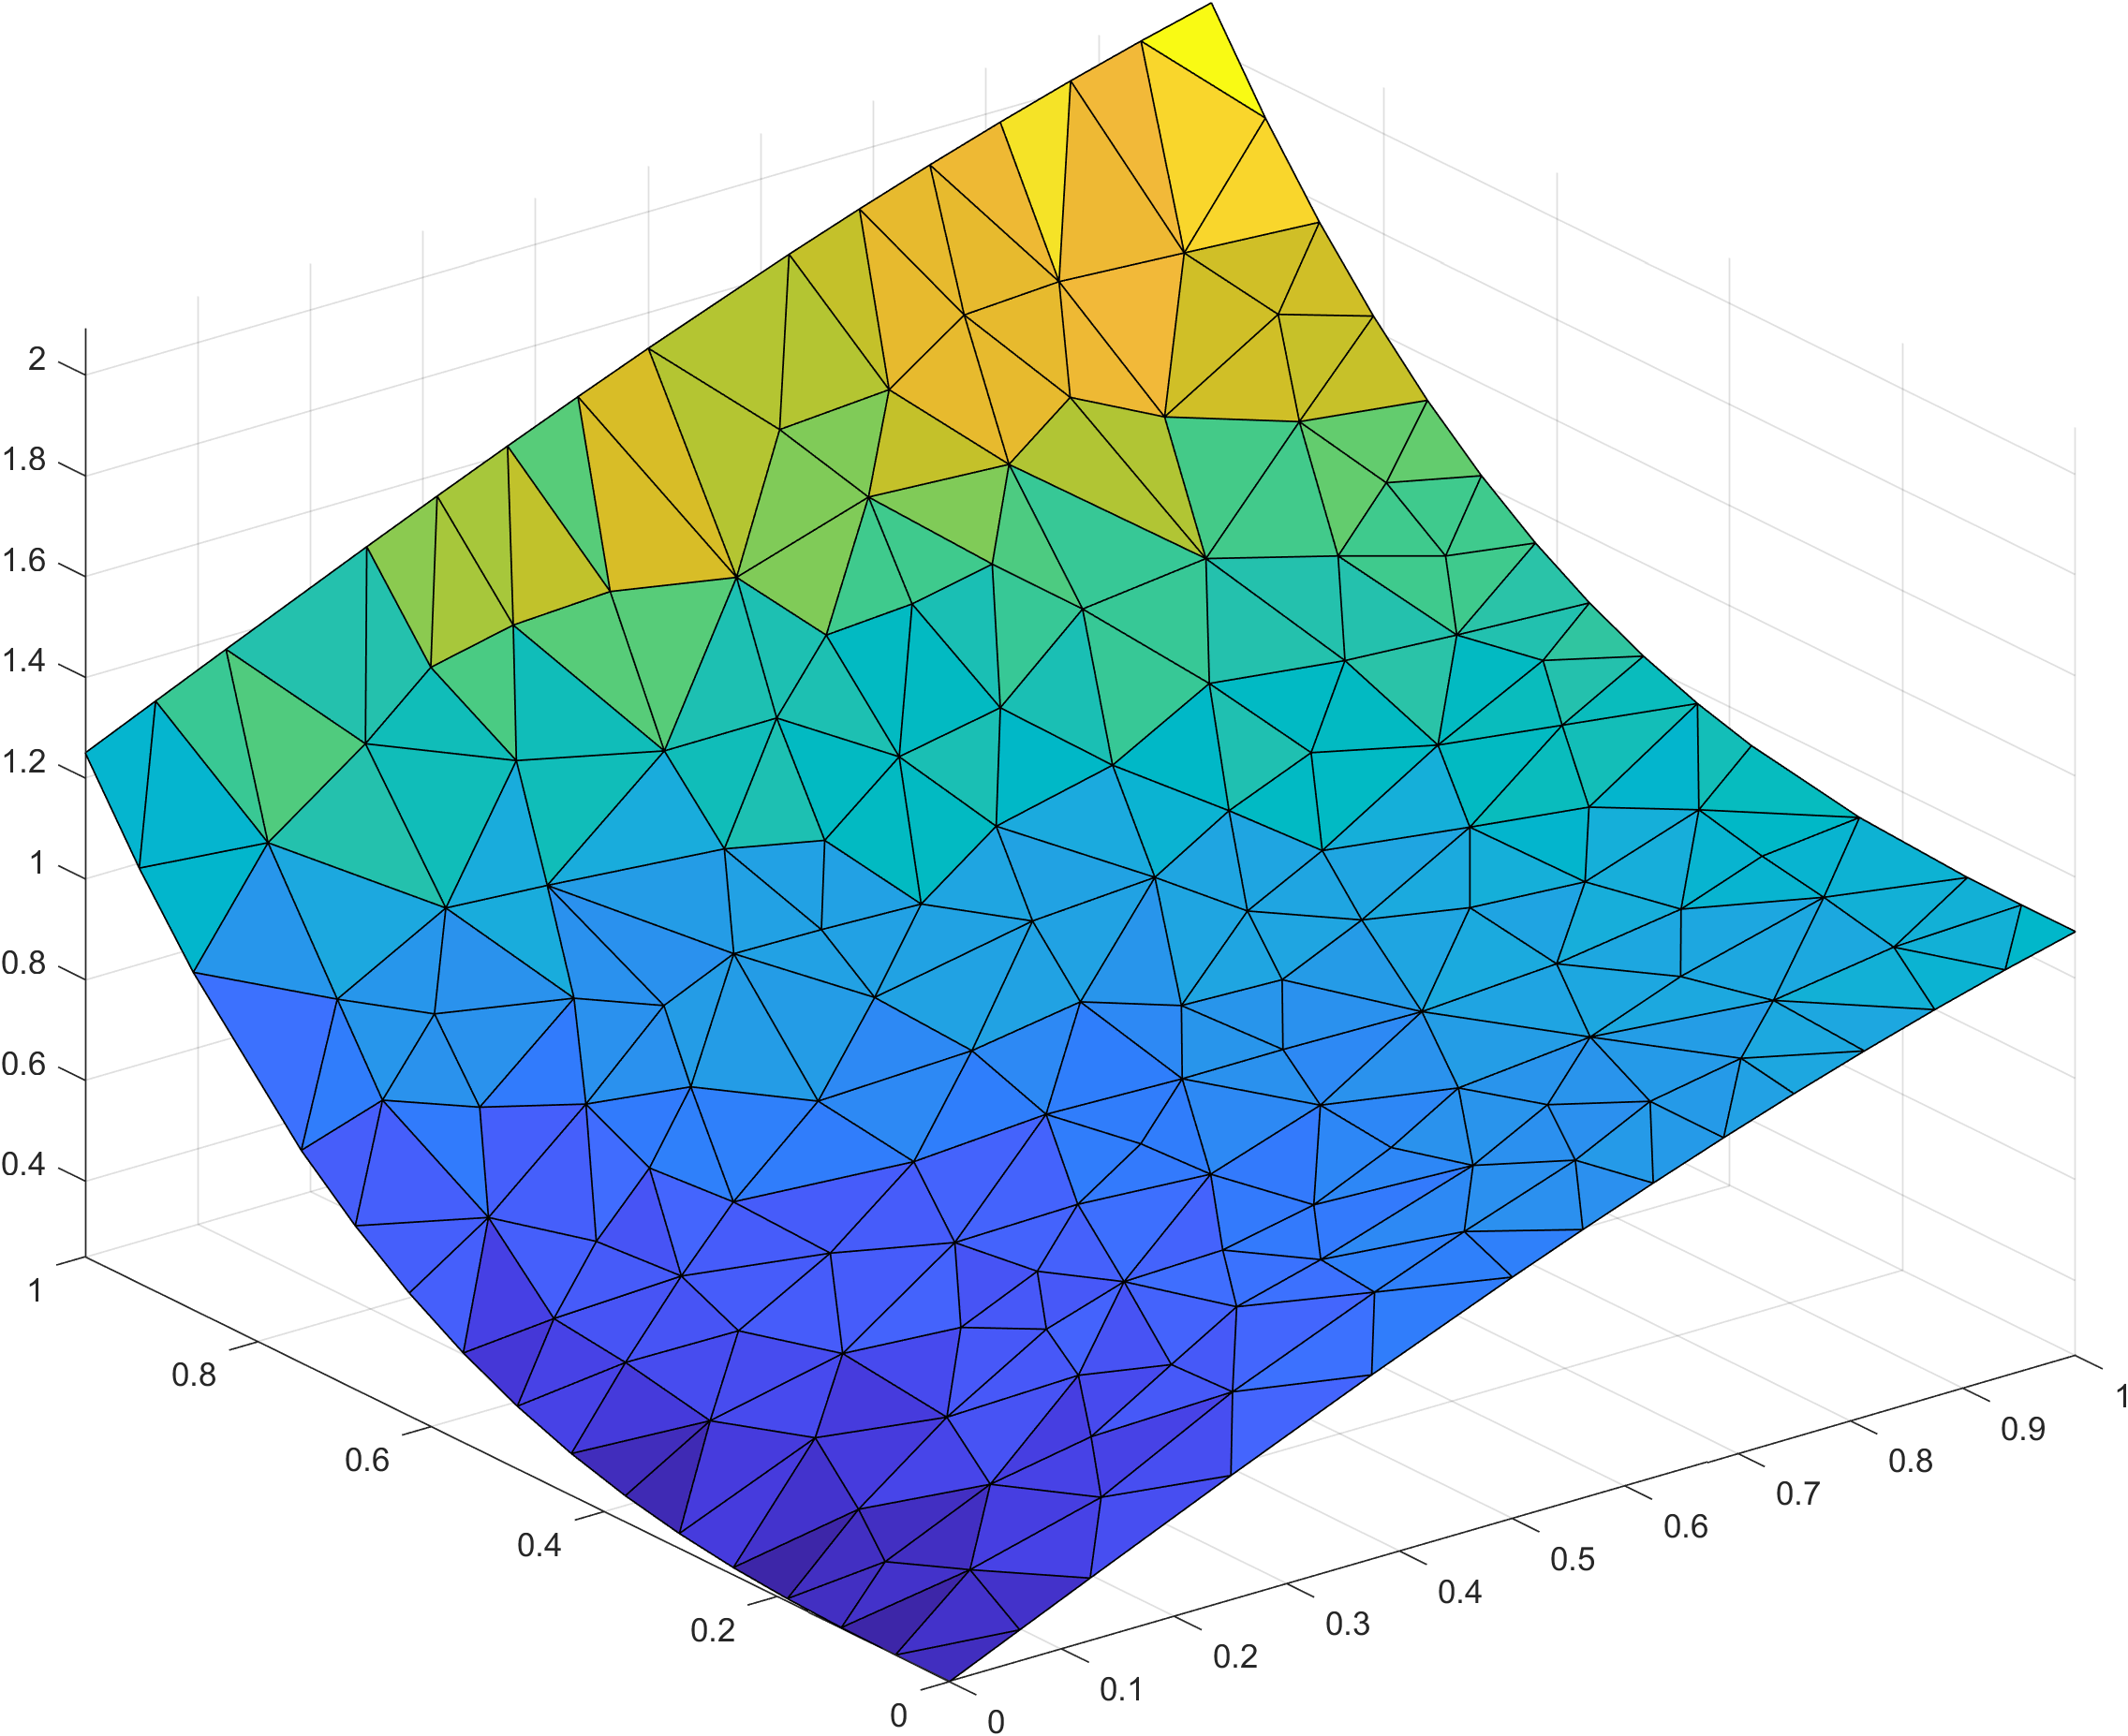
\includegraphics[height=\dimIm]{../Immagini/ES1_P1_AMax=dt=0.005_t=0.5.png}
                            \caption{Soluzione qualitativa coi $\mathbb{P}_1$ al tempo $t=0.5$.}
                            \label{figES1TriangolazioniP1TM}
                        \end{subfigure}
                        \begin{subfigure}[t]{\lungSF}
                            \centering
                            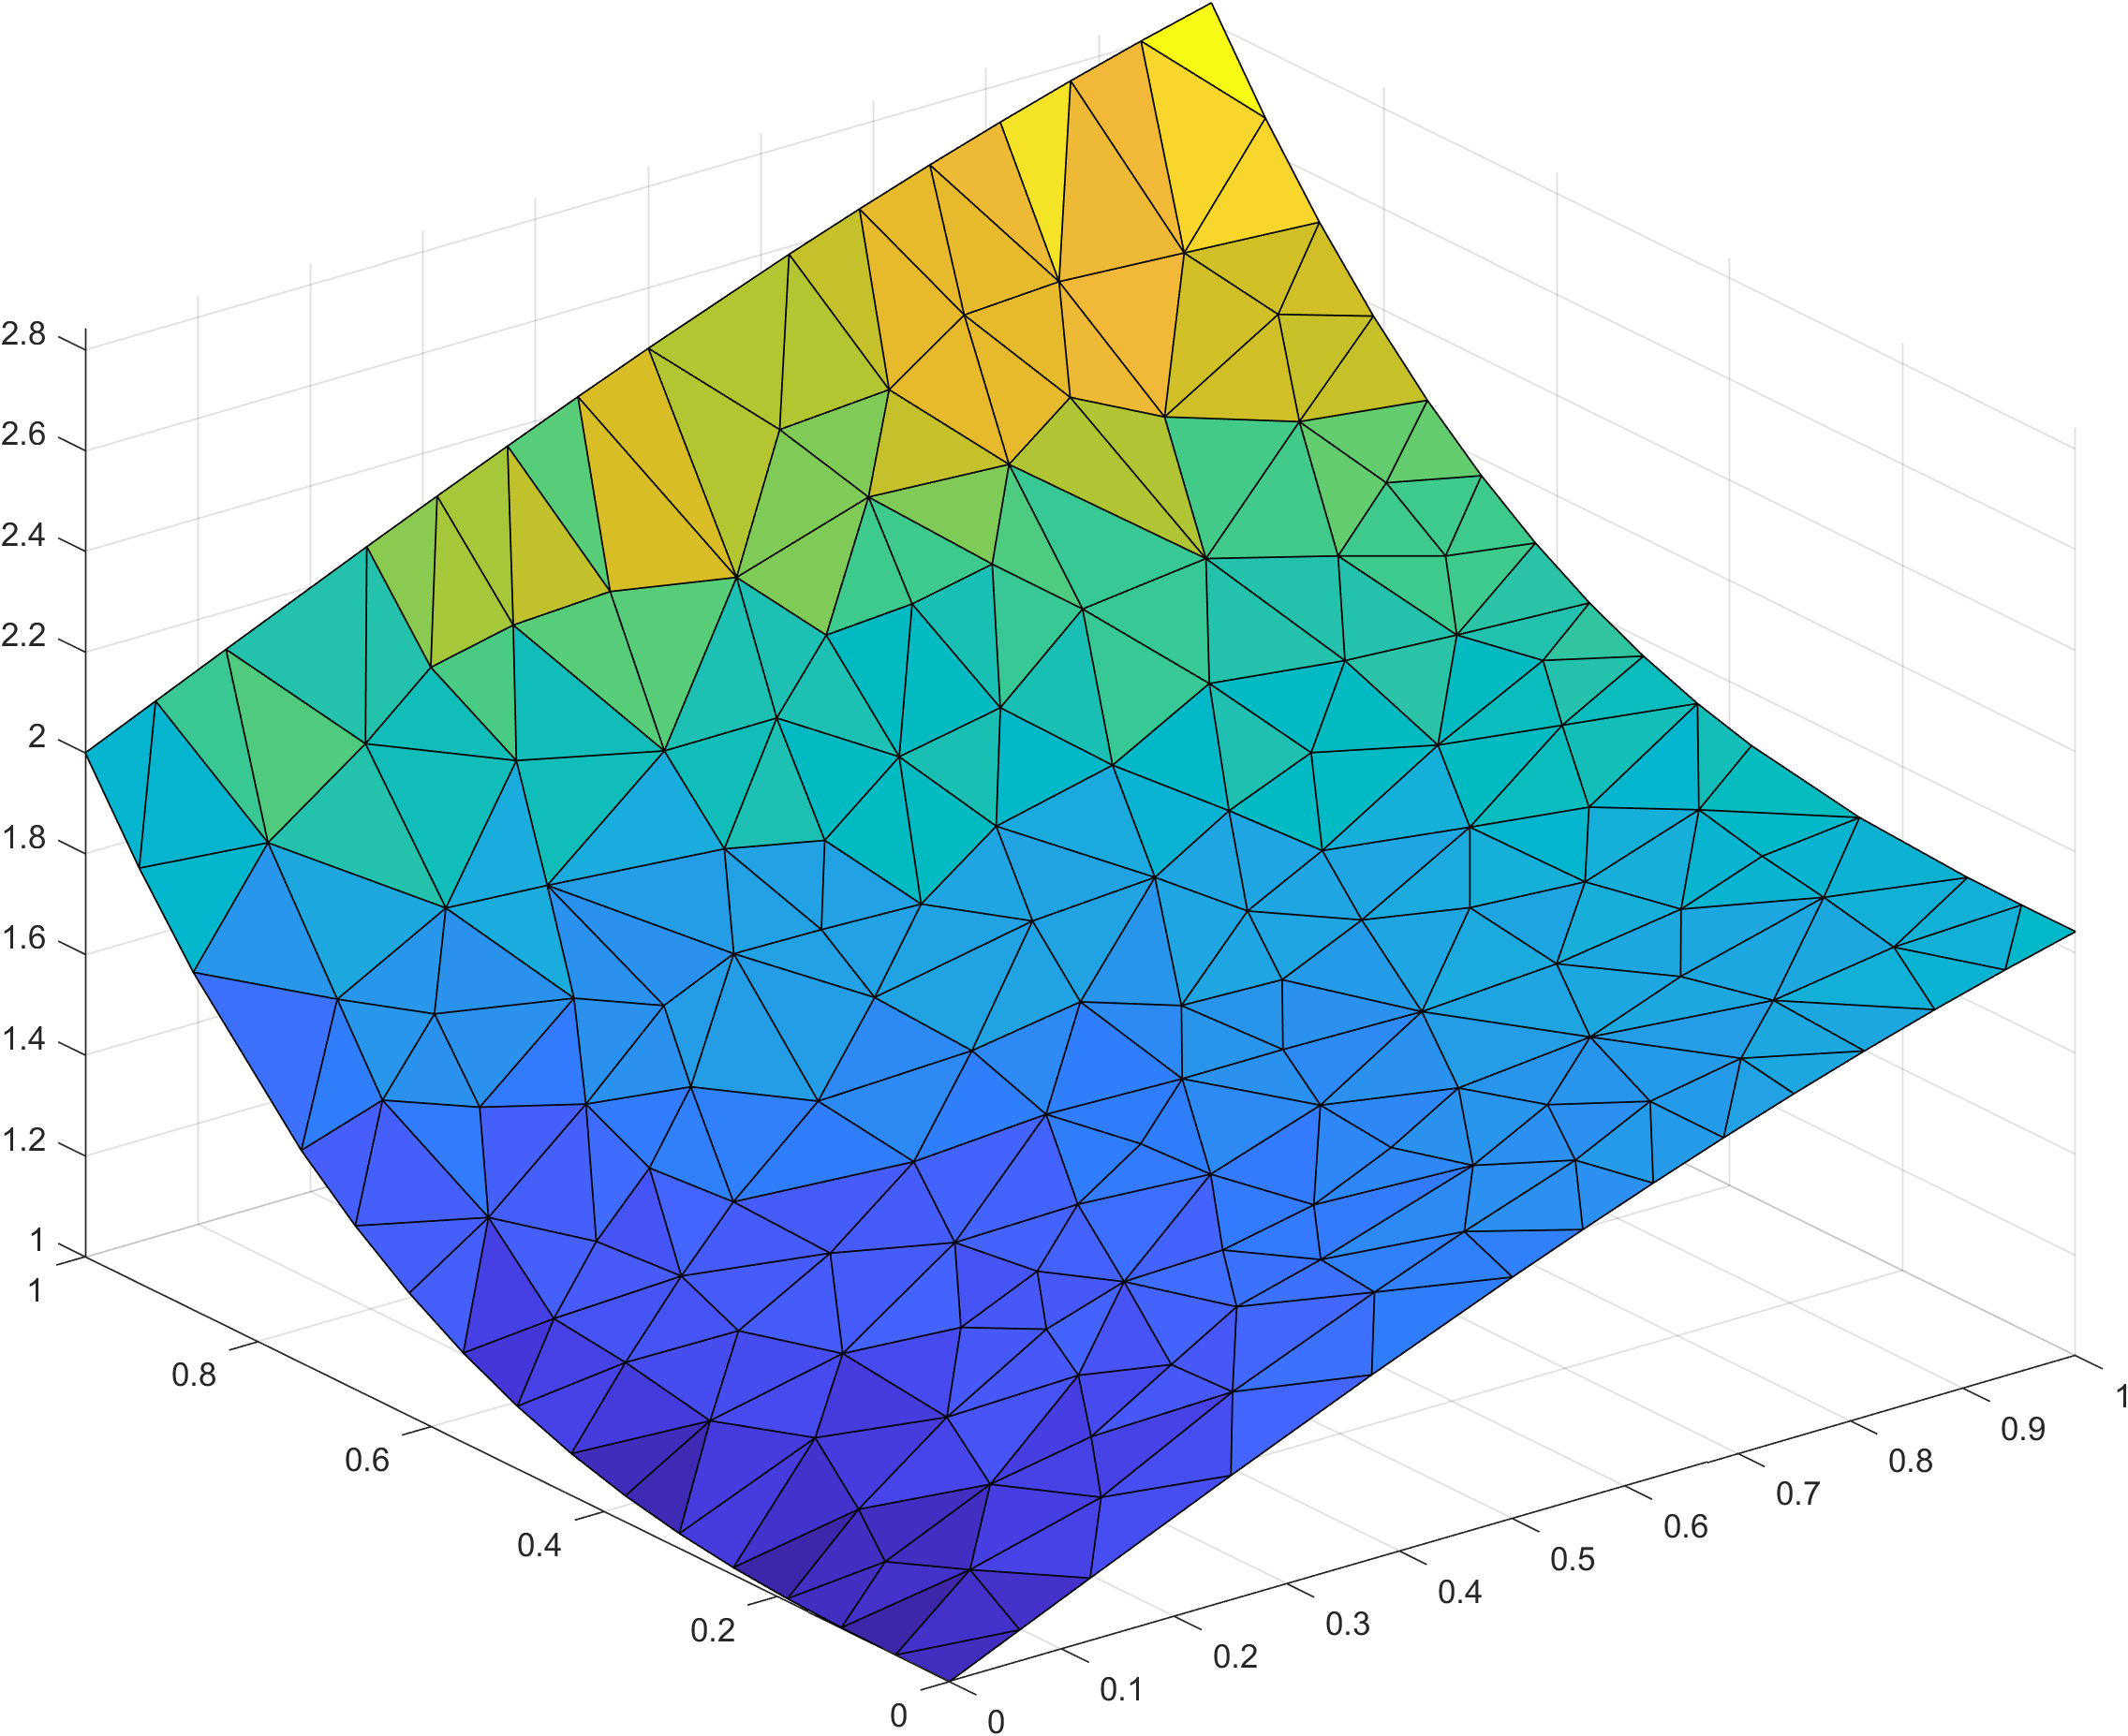
\includegraphics[height=\dimIm]{../Immagini/ES1_P1_AMax=dt=0.005_t=1.png}
                            \caption{Soluzione qualitativa coi $\mathbb{P}_1$ al tempo $t=1$.}
                            \label{figES1TriangolazioniP1TF}
                        \end{subfigure}
                    }
                    \distR
        
                    \renewcommand{\lungSF}{.5\linewidth}
                    \renewcommand{\dimIm}{\linewidth}
                    \newcommand{\distC}{\hspace{7.5pt}} % Distanza tra le colonne
                    \makebox[\linewidth][c]{
                        \begin{subfigure}[c]{\lungSF}
                            \centering
                            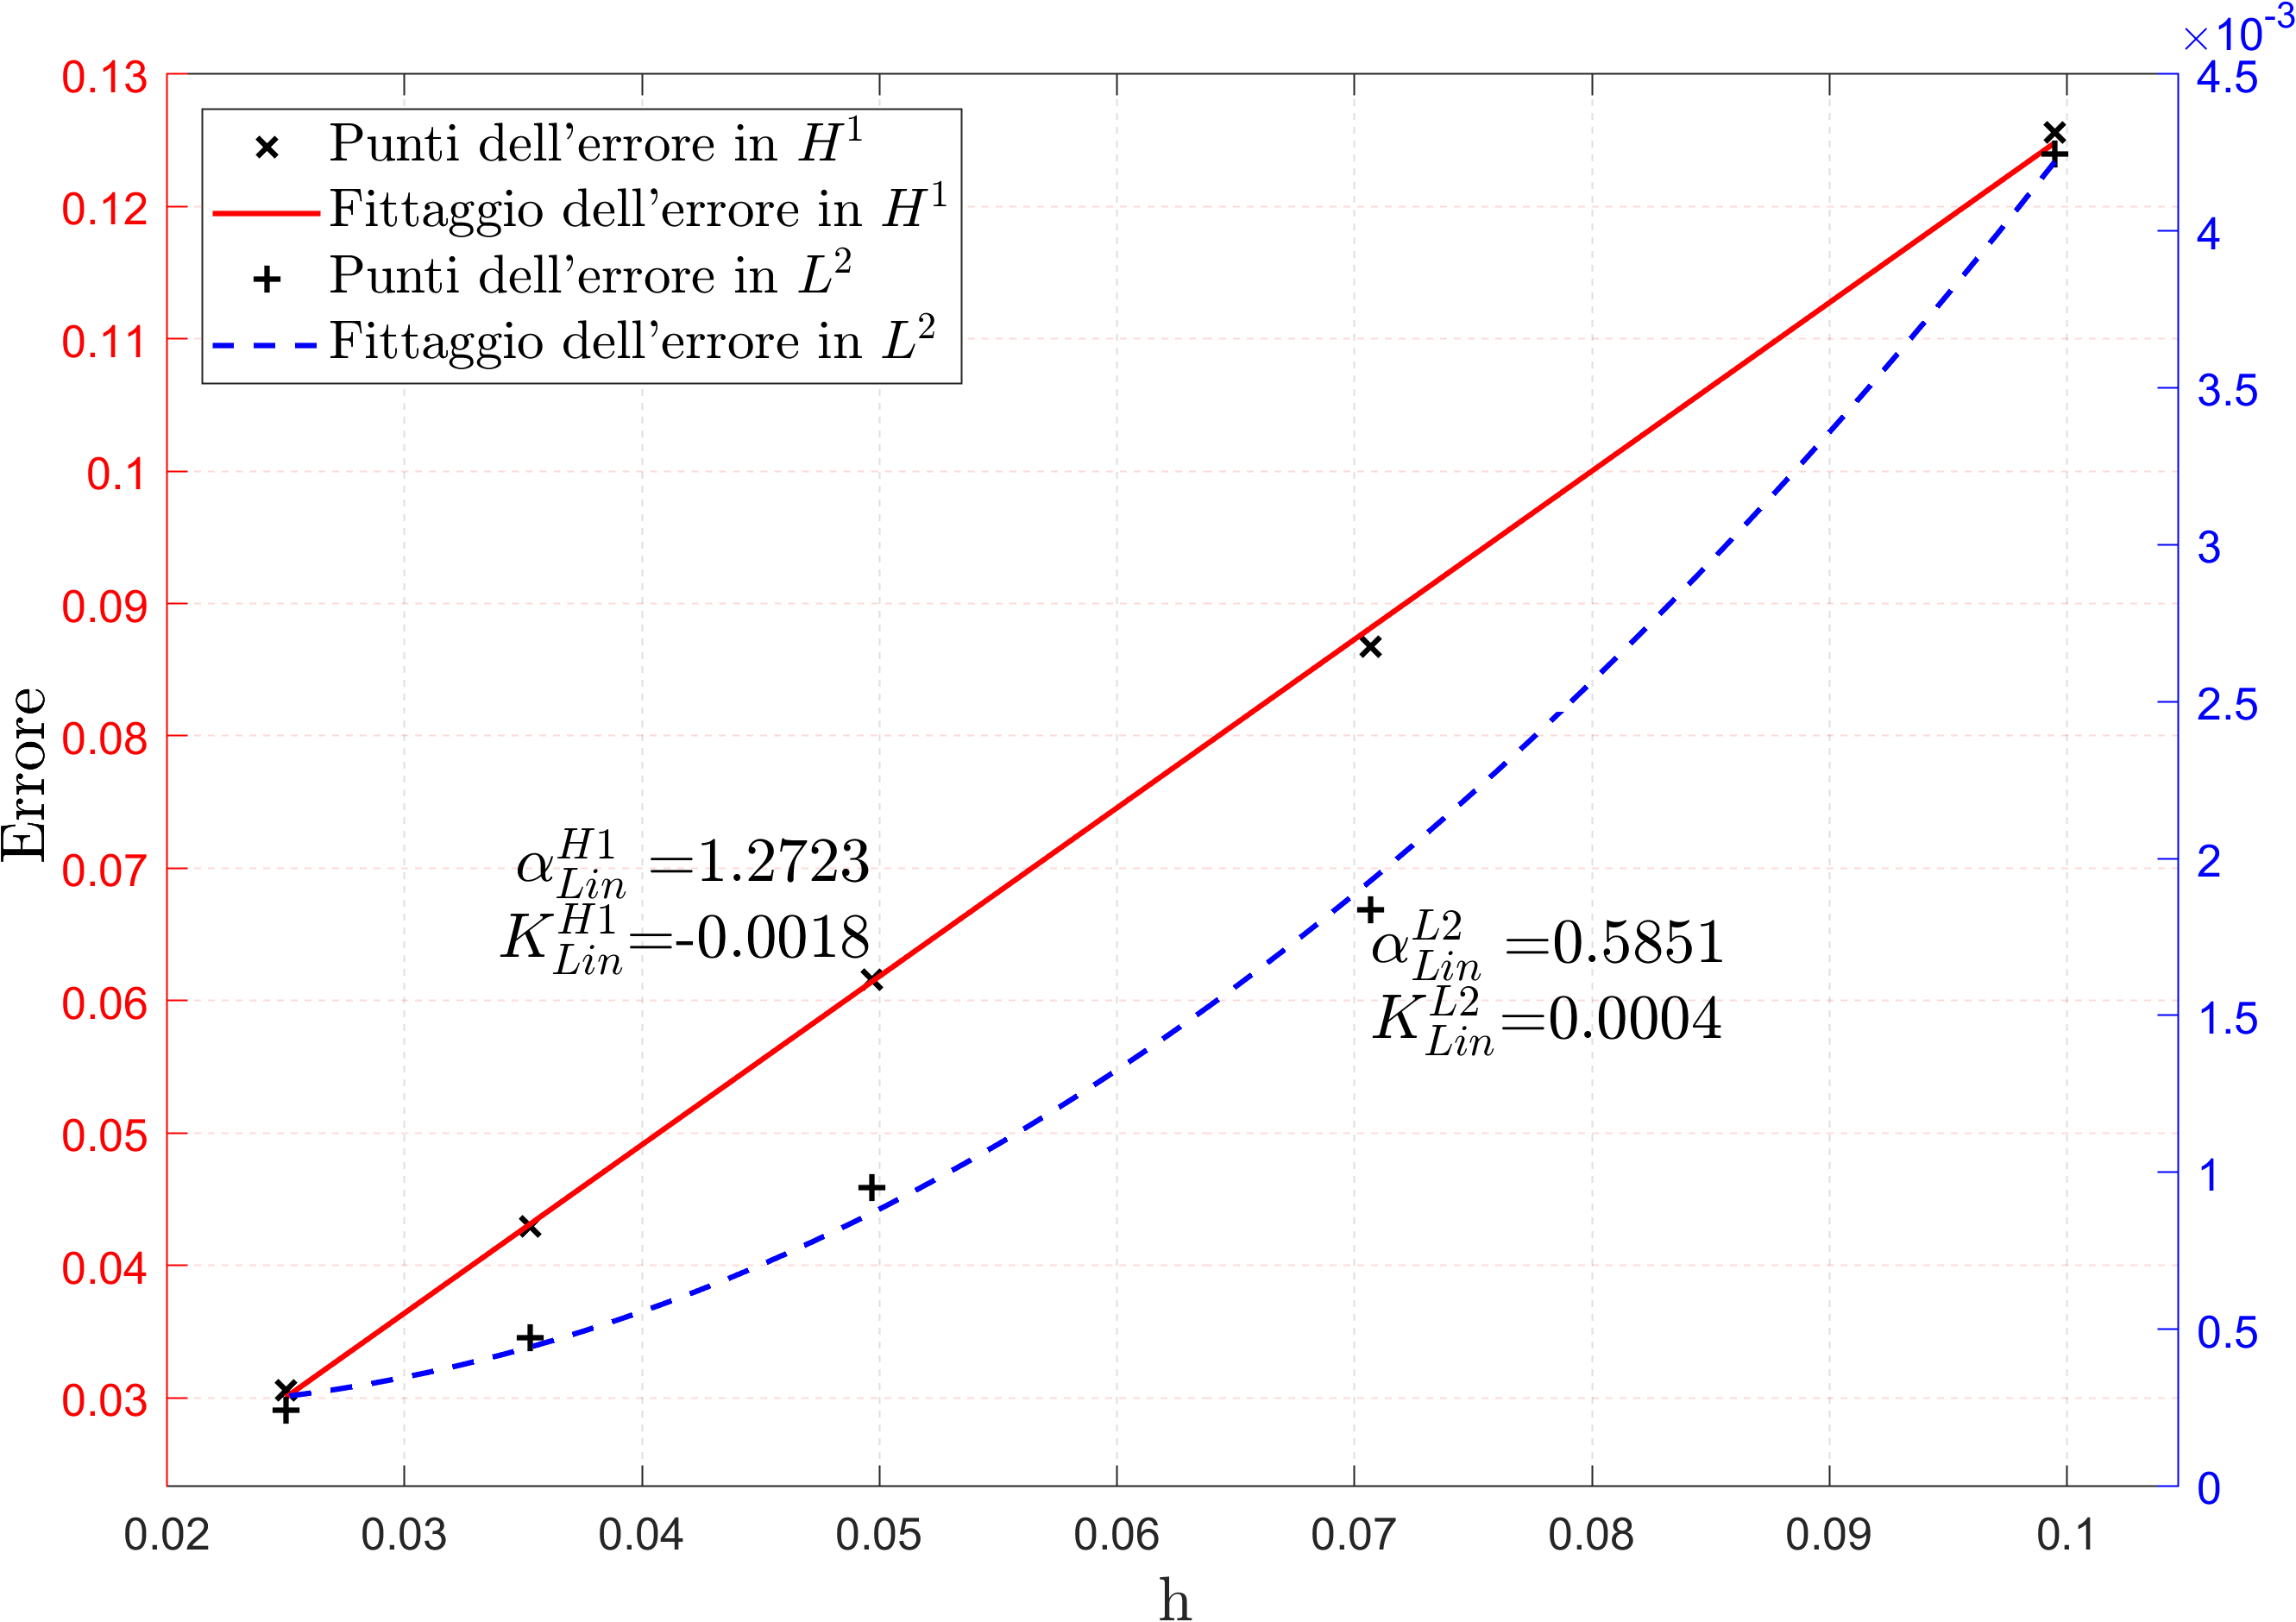
\includegraphics[width=\dimIm]{../Immagini/ES1_P1_ErrLin_AMax=dt=0.01_NSim=5.png}
                        \caption{Errore dei $\mathbb{P}_1$ in scala lineare.}
                        \label{figES1ErroreP1Lin}
                        \end{subfigure}
                        \distC
                        \begin{subfigure}[c]{\lungSF}
                            \centering
                            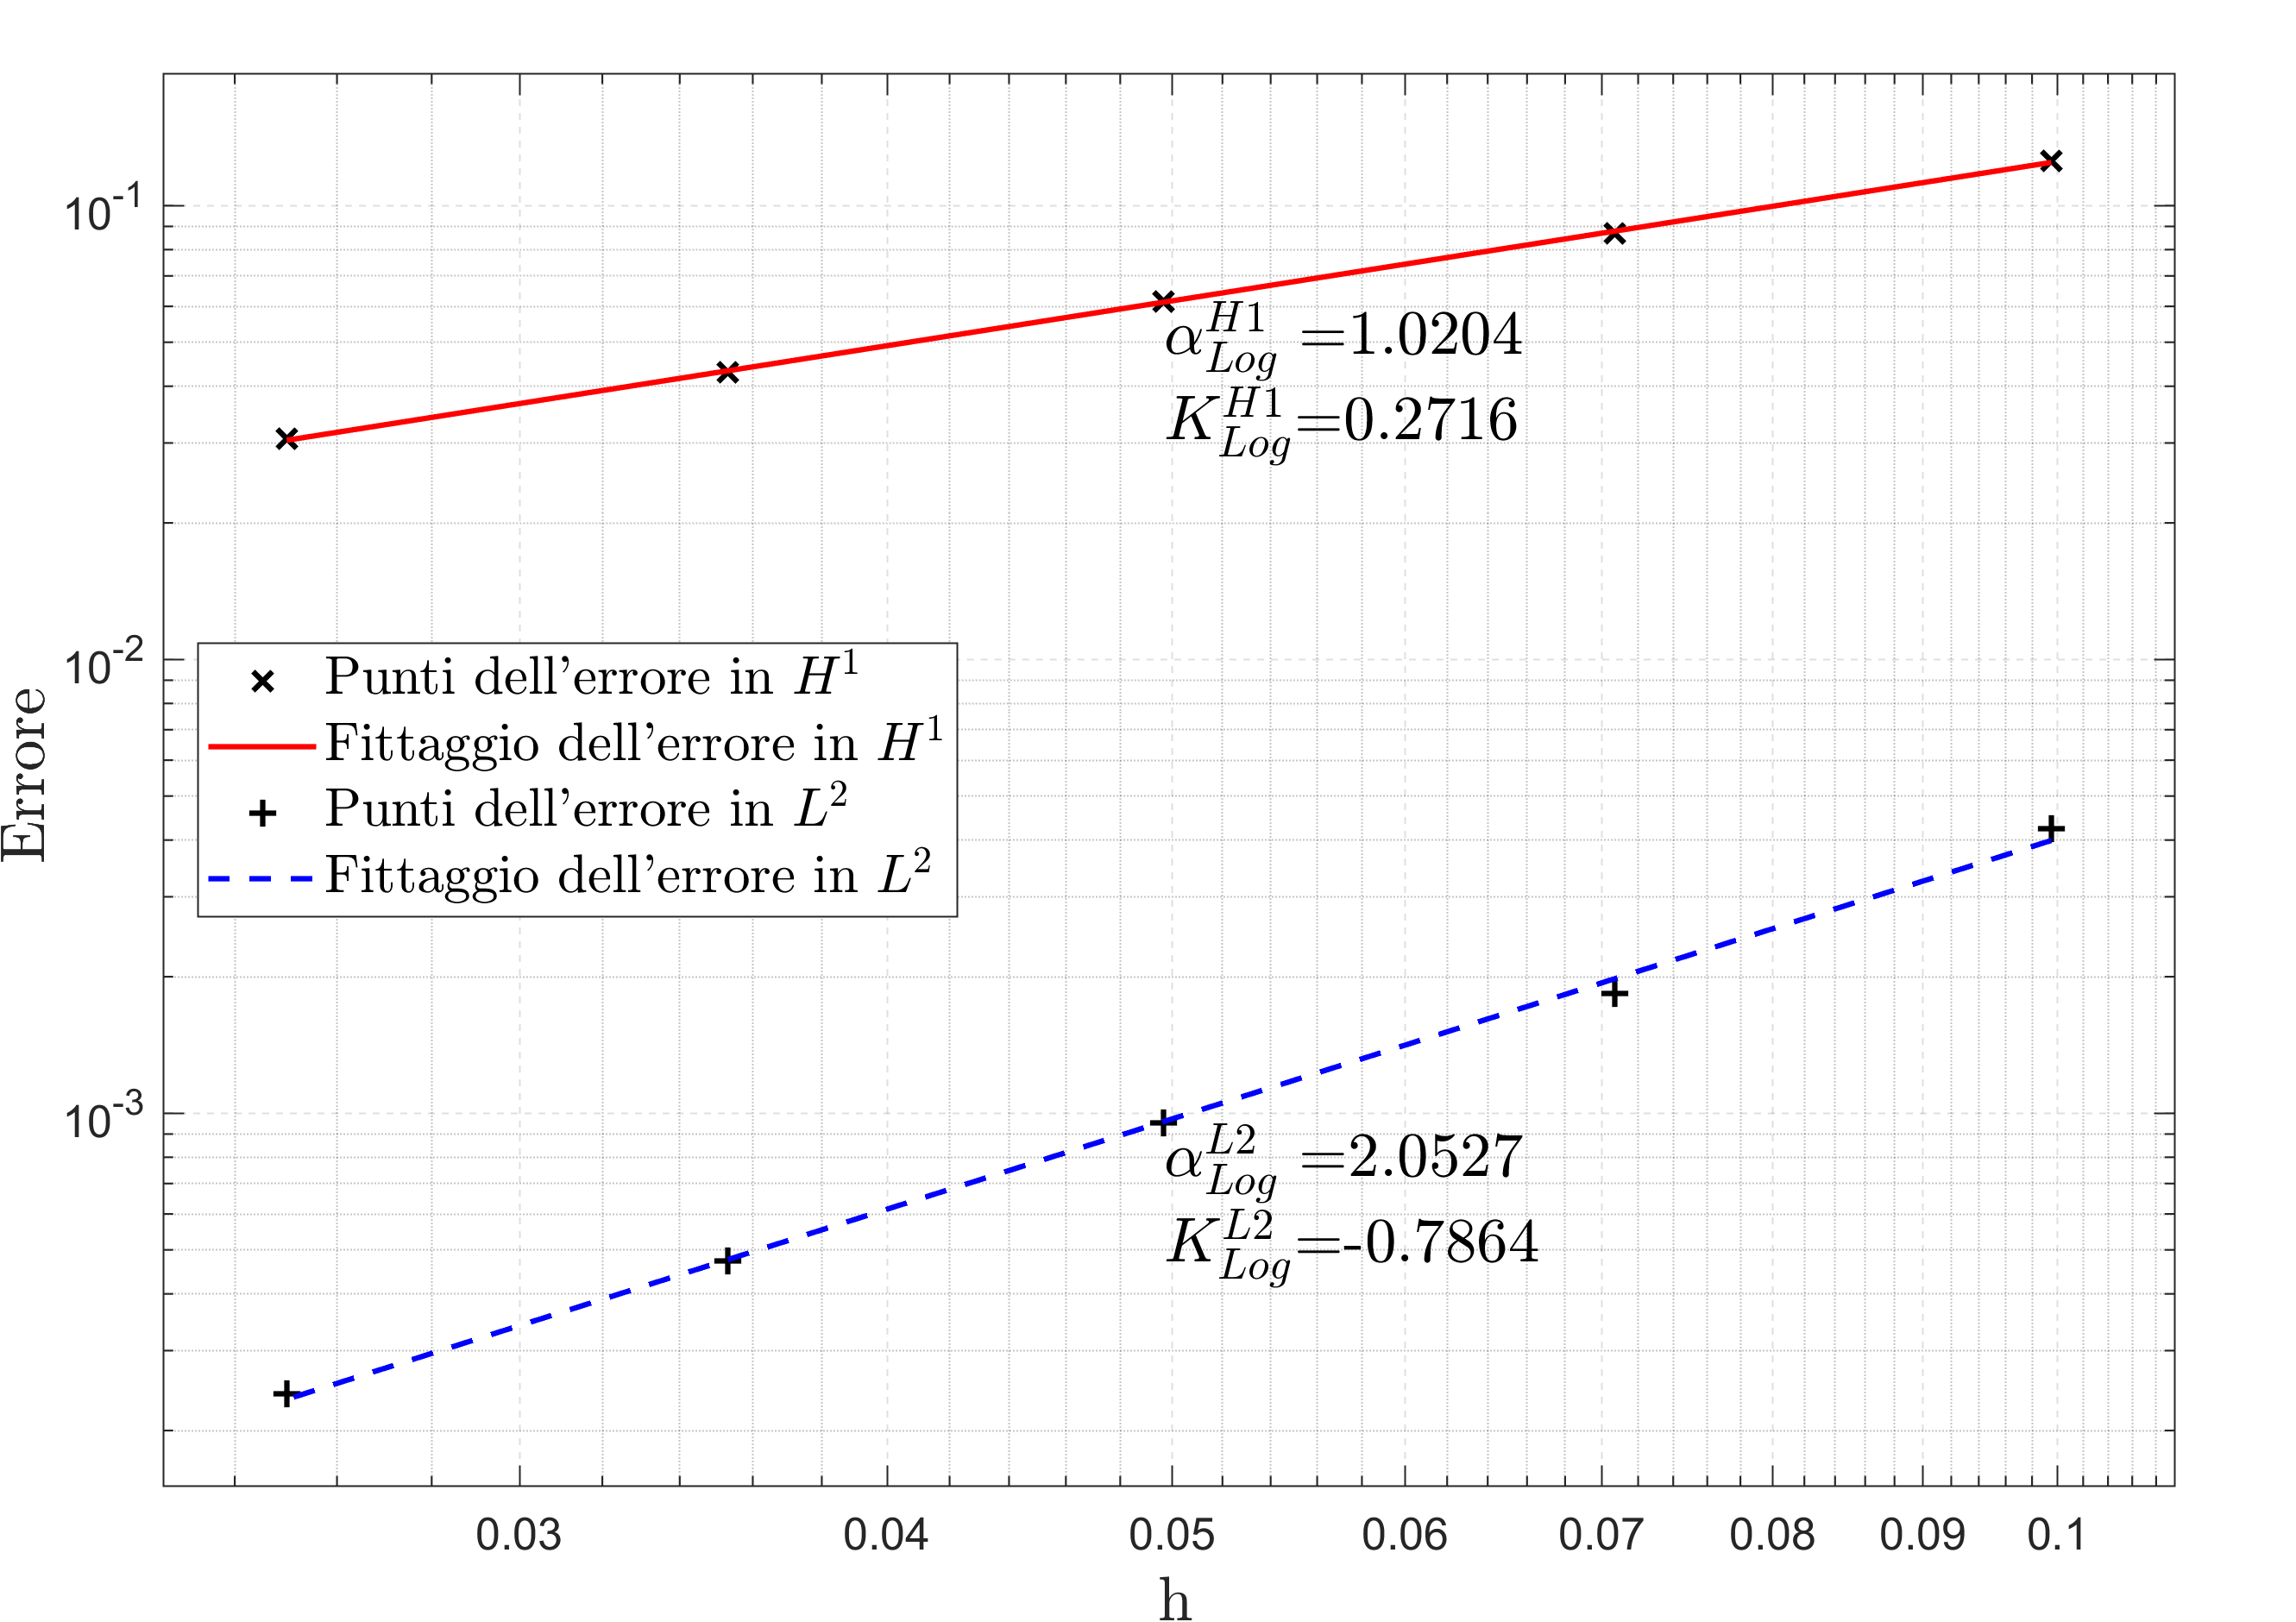
\includegraphics[width=\dimIm]{../Immagini/ES1_P1_ErrLog_AMax=dt=0.01_NSim=5.png}
                        \caption{Errore dei $\mathbb{P}_1$ in scala logaritmica.}
                        \label{figES1ErroreP1Log}
                        \end{subfigure}
                    }
                    \caption{Nelle Figg. \ref{figES1TriangolazioniEsattaTI}-\ref{figES1TriangolazioniP1TF} sono mostrate le soluzioni dell'ES1 in tre istanti temporali: le prime tre mostrano la soluzione esatta e le restanti quella approssimata; invece nelle \ref{figES1ErroreP1Lin} e \ref{figES1ErroreP1Log} sono illustrati in due scale diverse gli errori in norma $H^1$ ed $L^2$. I parametri dati a \textit{BBTR} sono spiegati nel $\S$\ref{parPremessaParametriBBTR}.}
                    \label{figES1}
                \end{figure*}
                %%%%%%%%%%%%%%%%%%
                %%%%%%%%%%%%%%%%%%
                %%%%%%%%%%%%%%%%%%

                %%%%%%%%%%%%%%%%%%%%%%
                %%% Infopagina ES2 %%%
                %%%%%%%%%%%%%%%%%%%%%%
                \begin{figure*}[p]
                    \newcommand{\distR}{\vspace{15pt}} % Distanza tra le righe
                    
                    \newcommand{\lungSF}{0.33\textwidth}
                    \newcommand{\dimIm}{4.6cm}
                    \makebox[\linewidth][c]{
                        % \captionsetup[subfigure]{width=2.4cm}
                        \SpaziaturaMate{1}{1}{1}
                        \begin{subfigure}[t]{\lungSF}
                            \centering
                            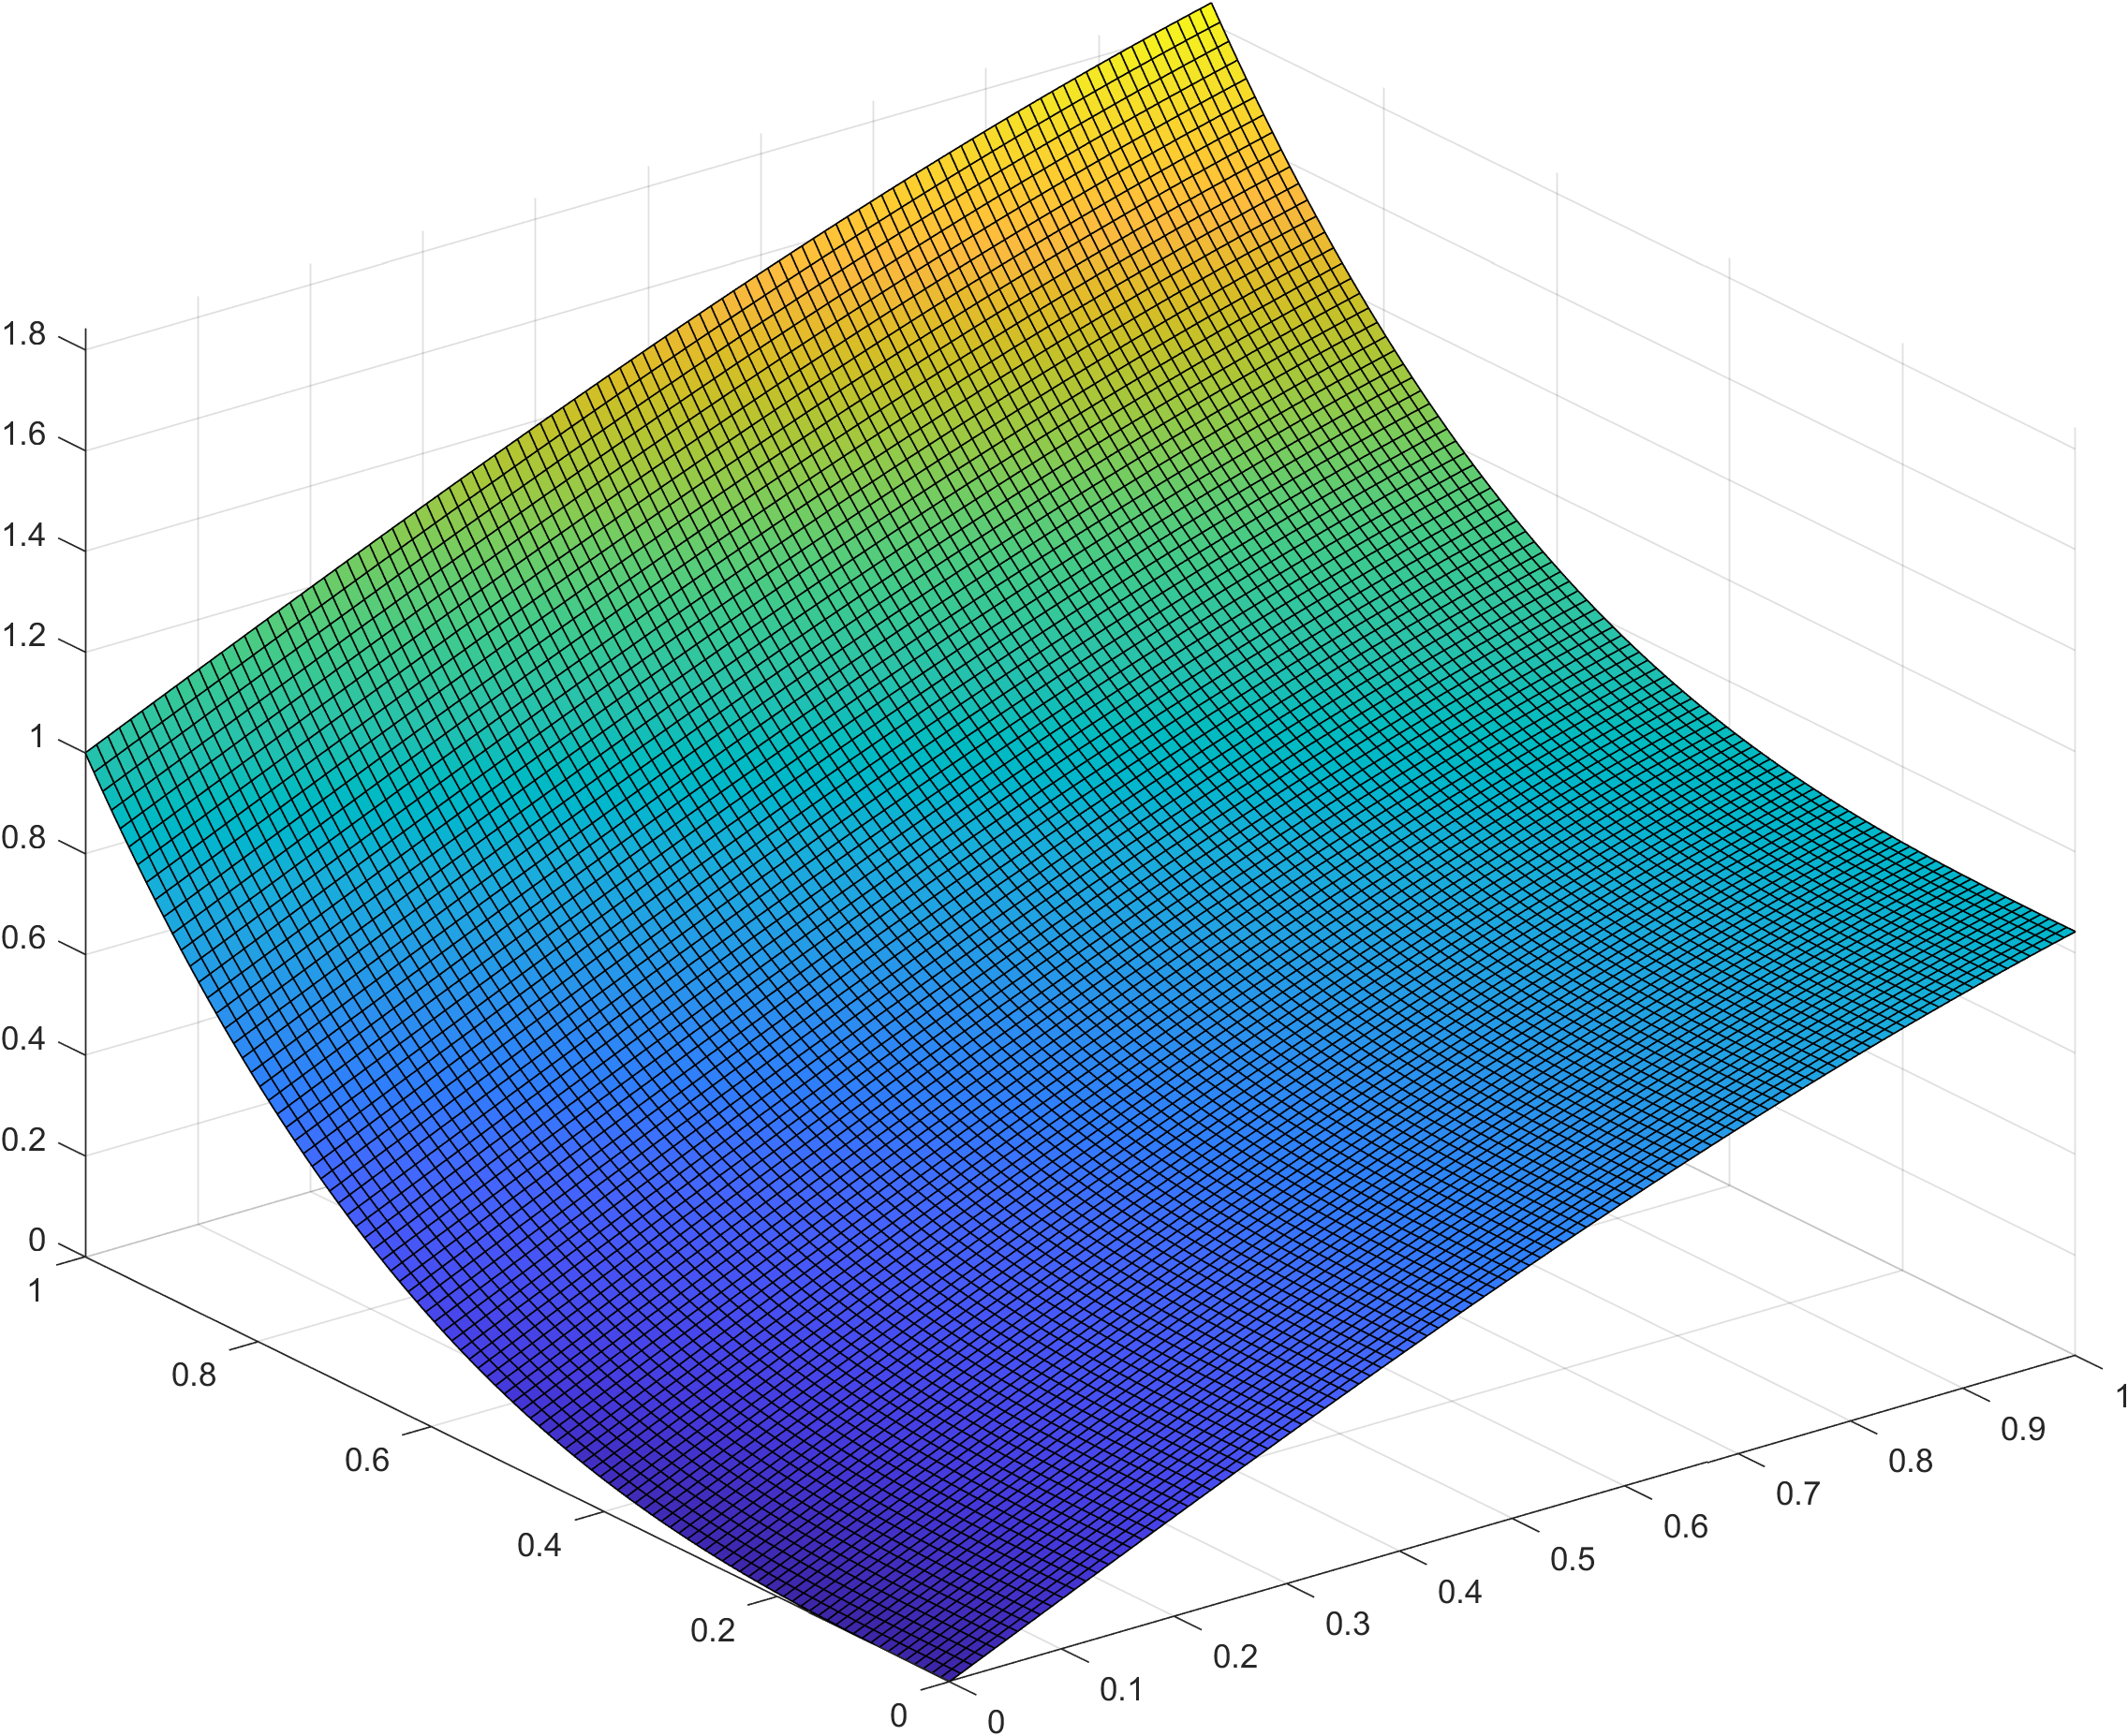
\includegraphics[height=\dimIm]{../Immagini/ES12_SE_NPunti=100_t=0.png}
                            \caption{Soluzione esatta al tempo $t=0$.}
                            \label{figES2TriangolazioniEsattaTI}
                        \end{subfigure}
                        \begin{subfigure}[t]{\lungSF}
                            \centering
                            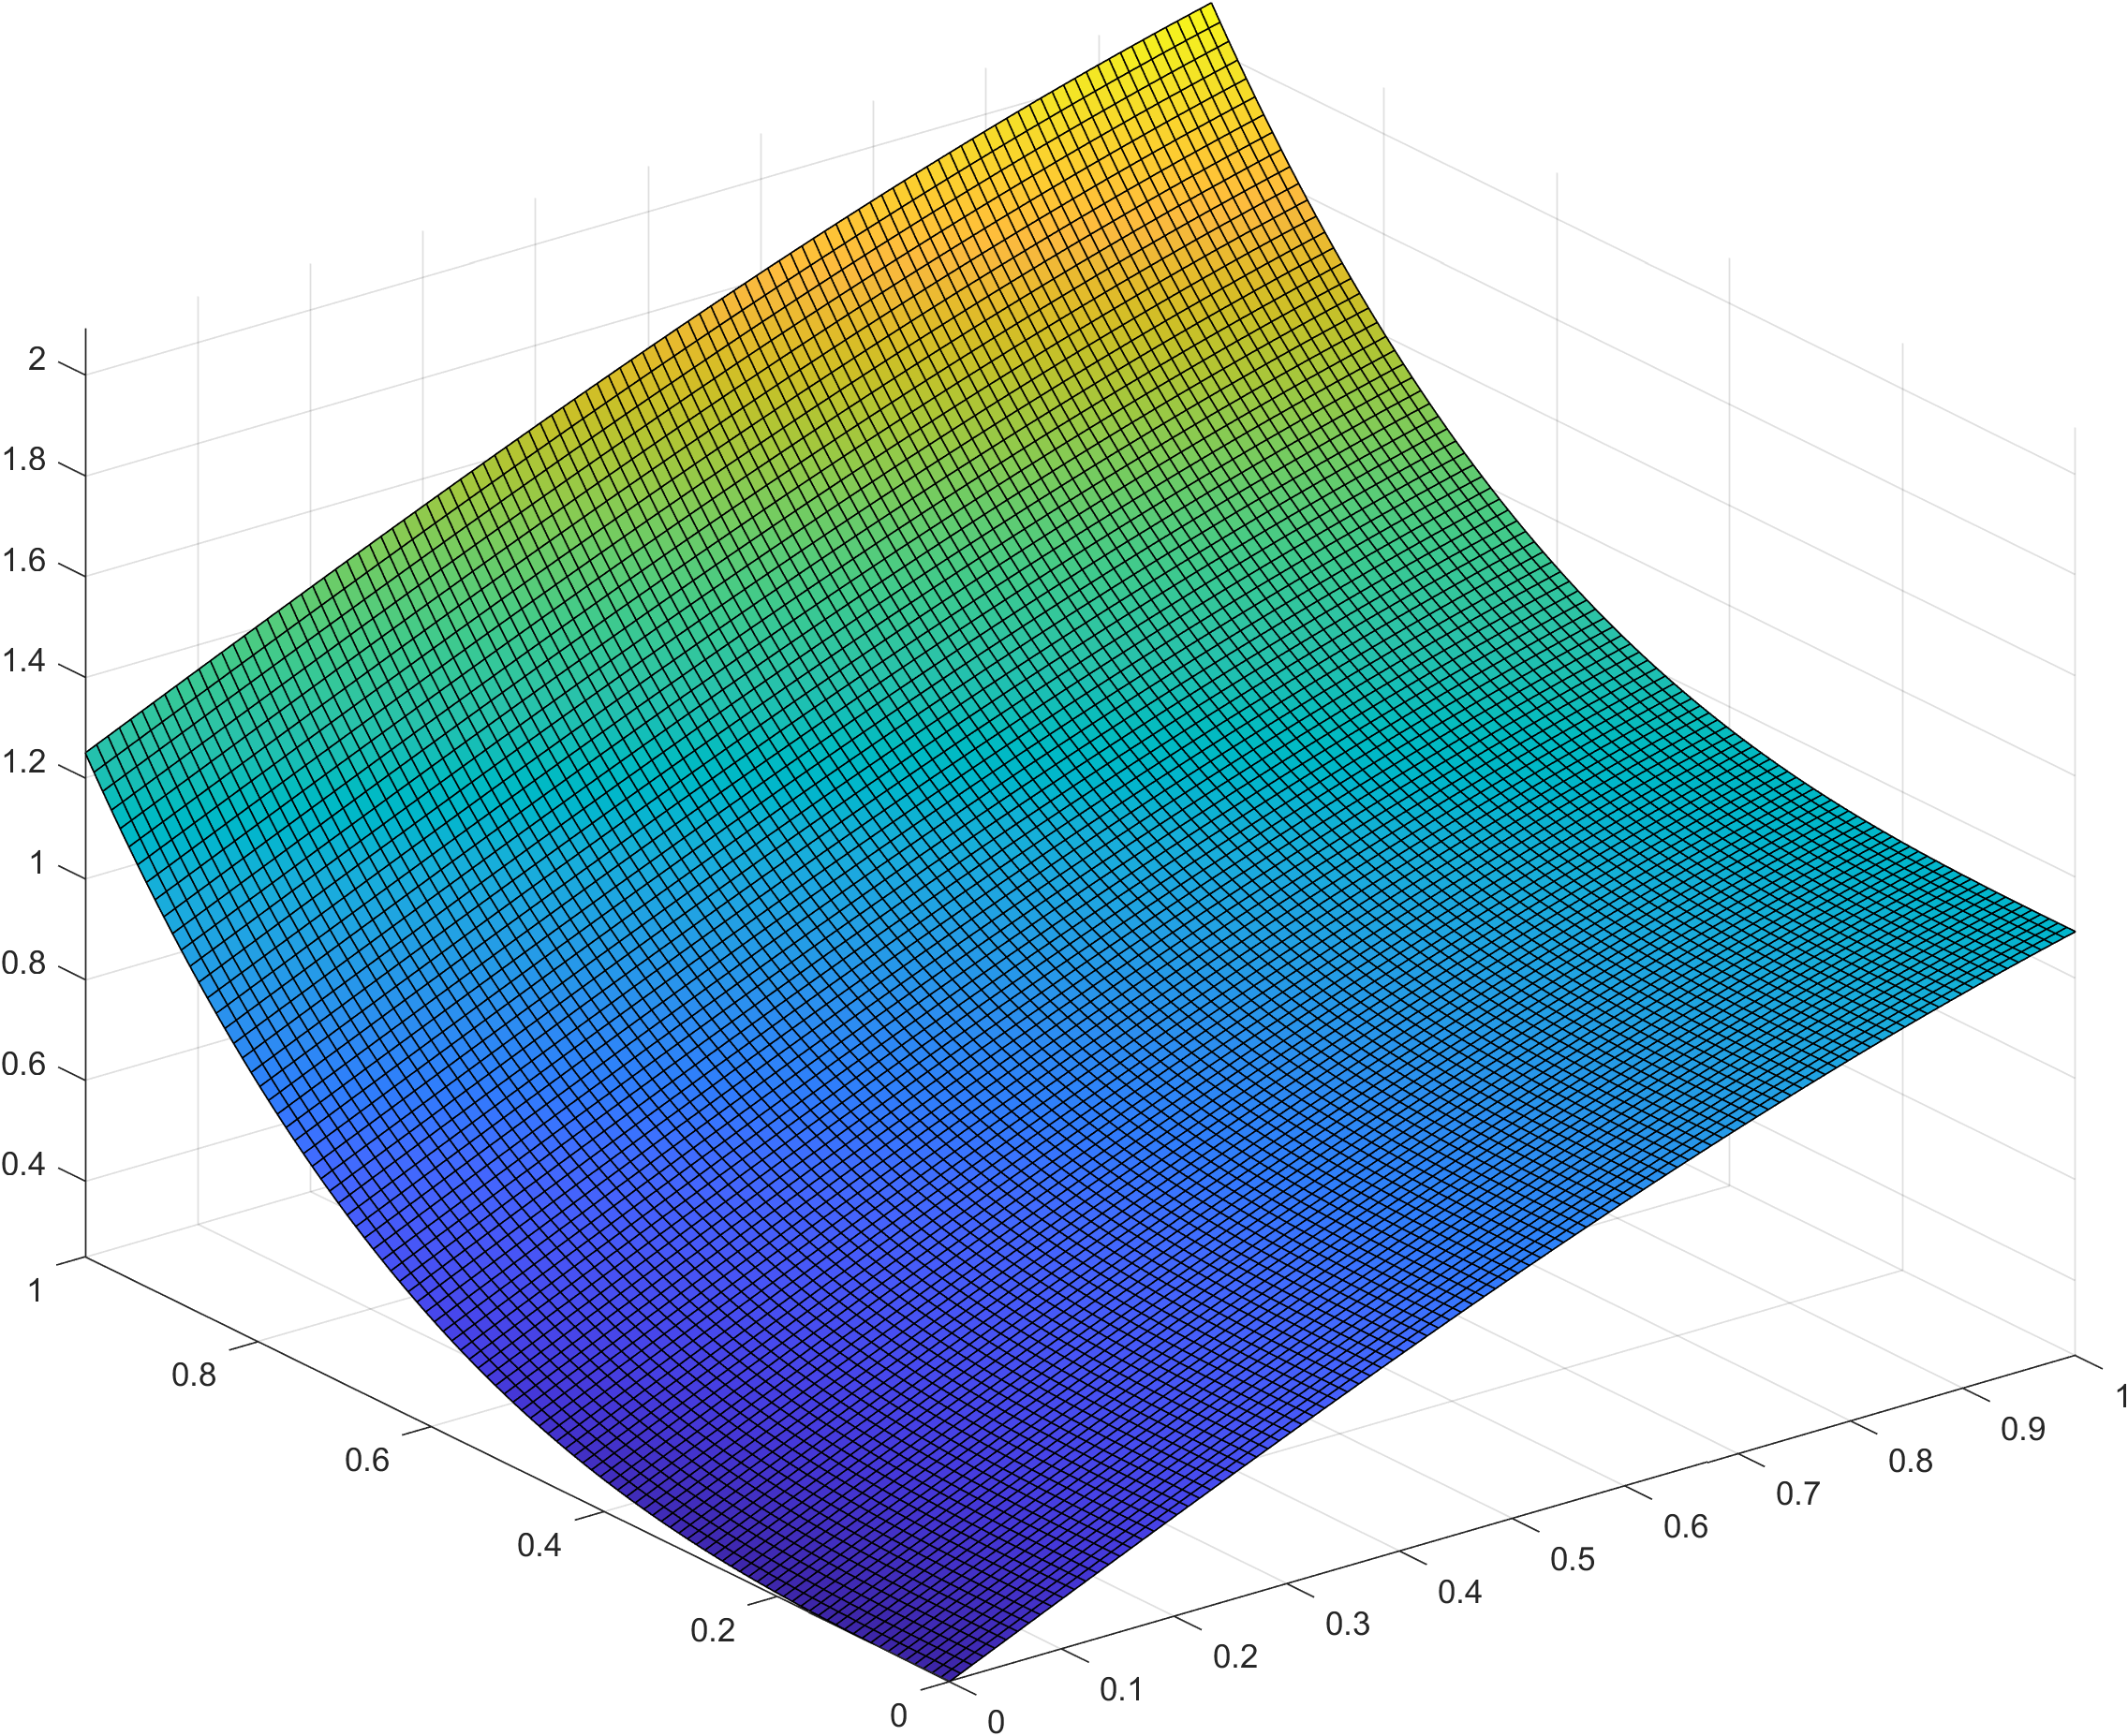
\includegraphics[height=\dimIm]{../Immagini/ES12_SE_NPunti=100_t=0.5.png}
                            \caption{Soluzione esatta al tempo $t=0.5$.}
                            \label{figES2TriangolazioniEsattaTM}
                        \end{subfigure}
                        \begin{subfigure}[t]{\lungSF}
                            \centering
                            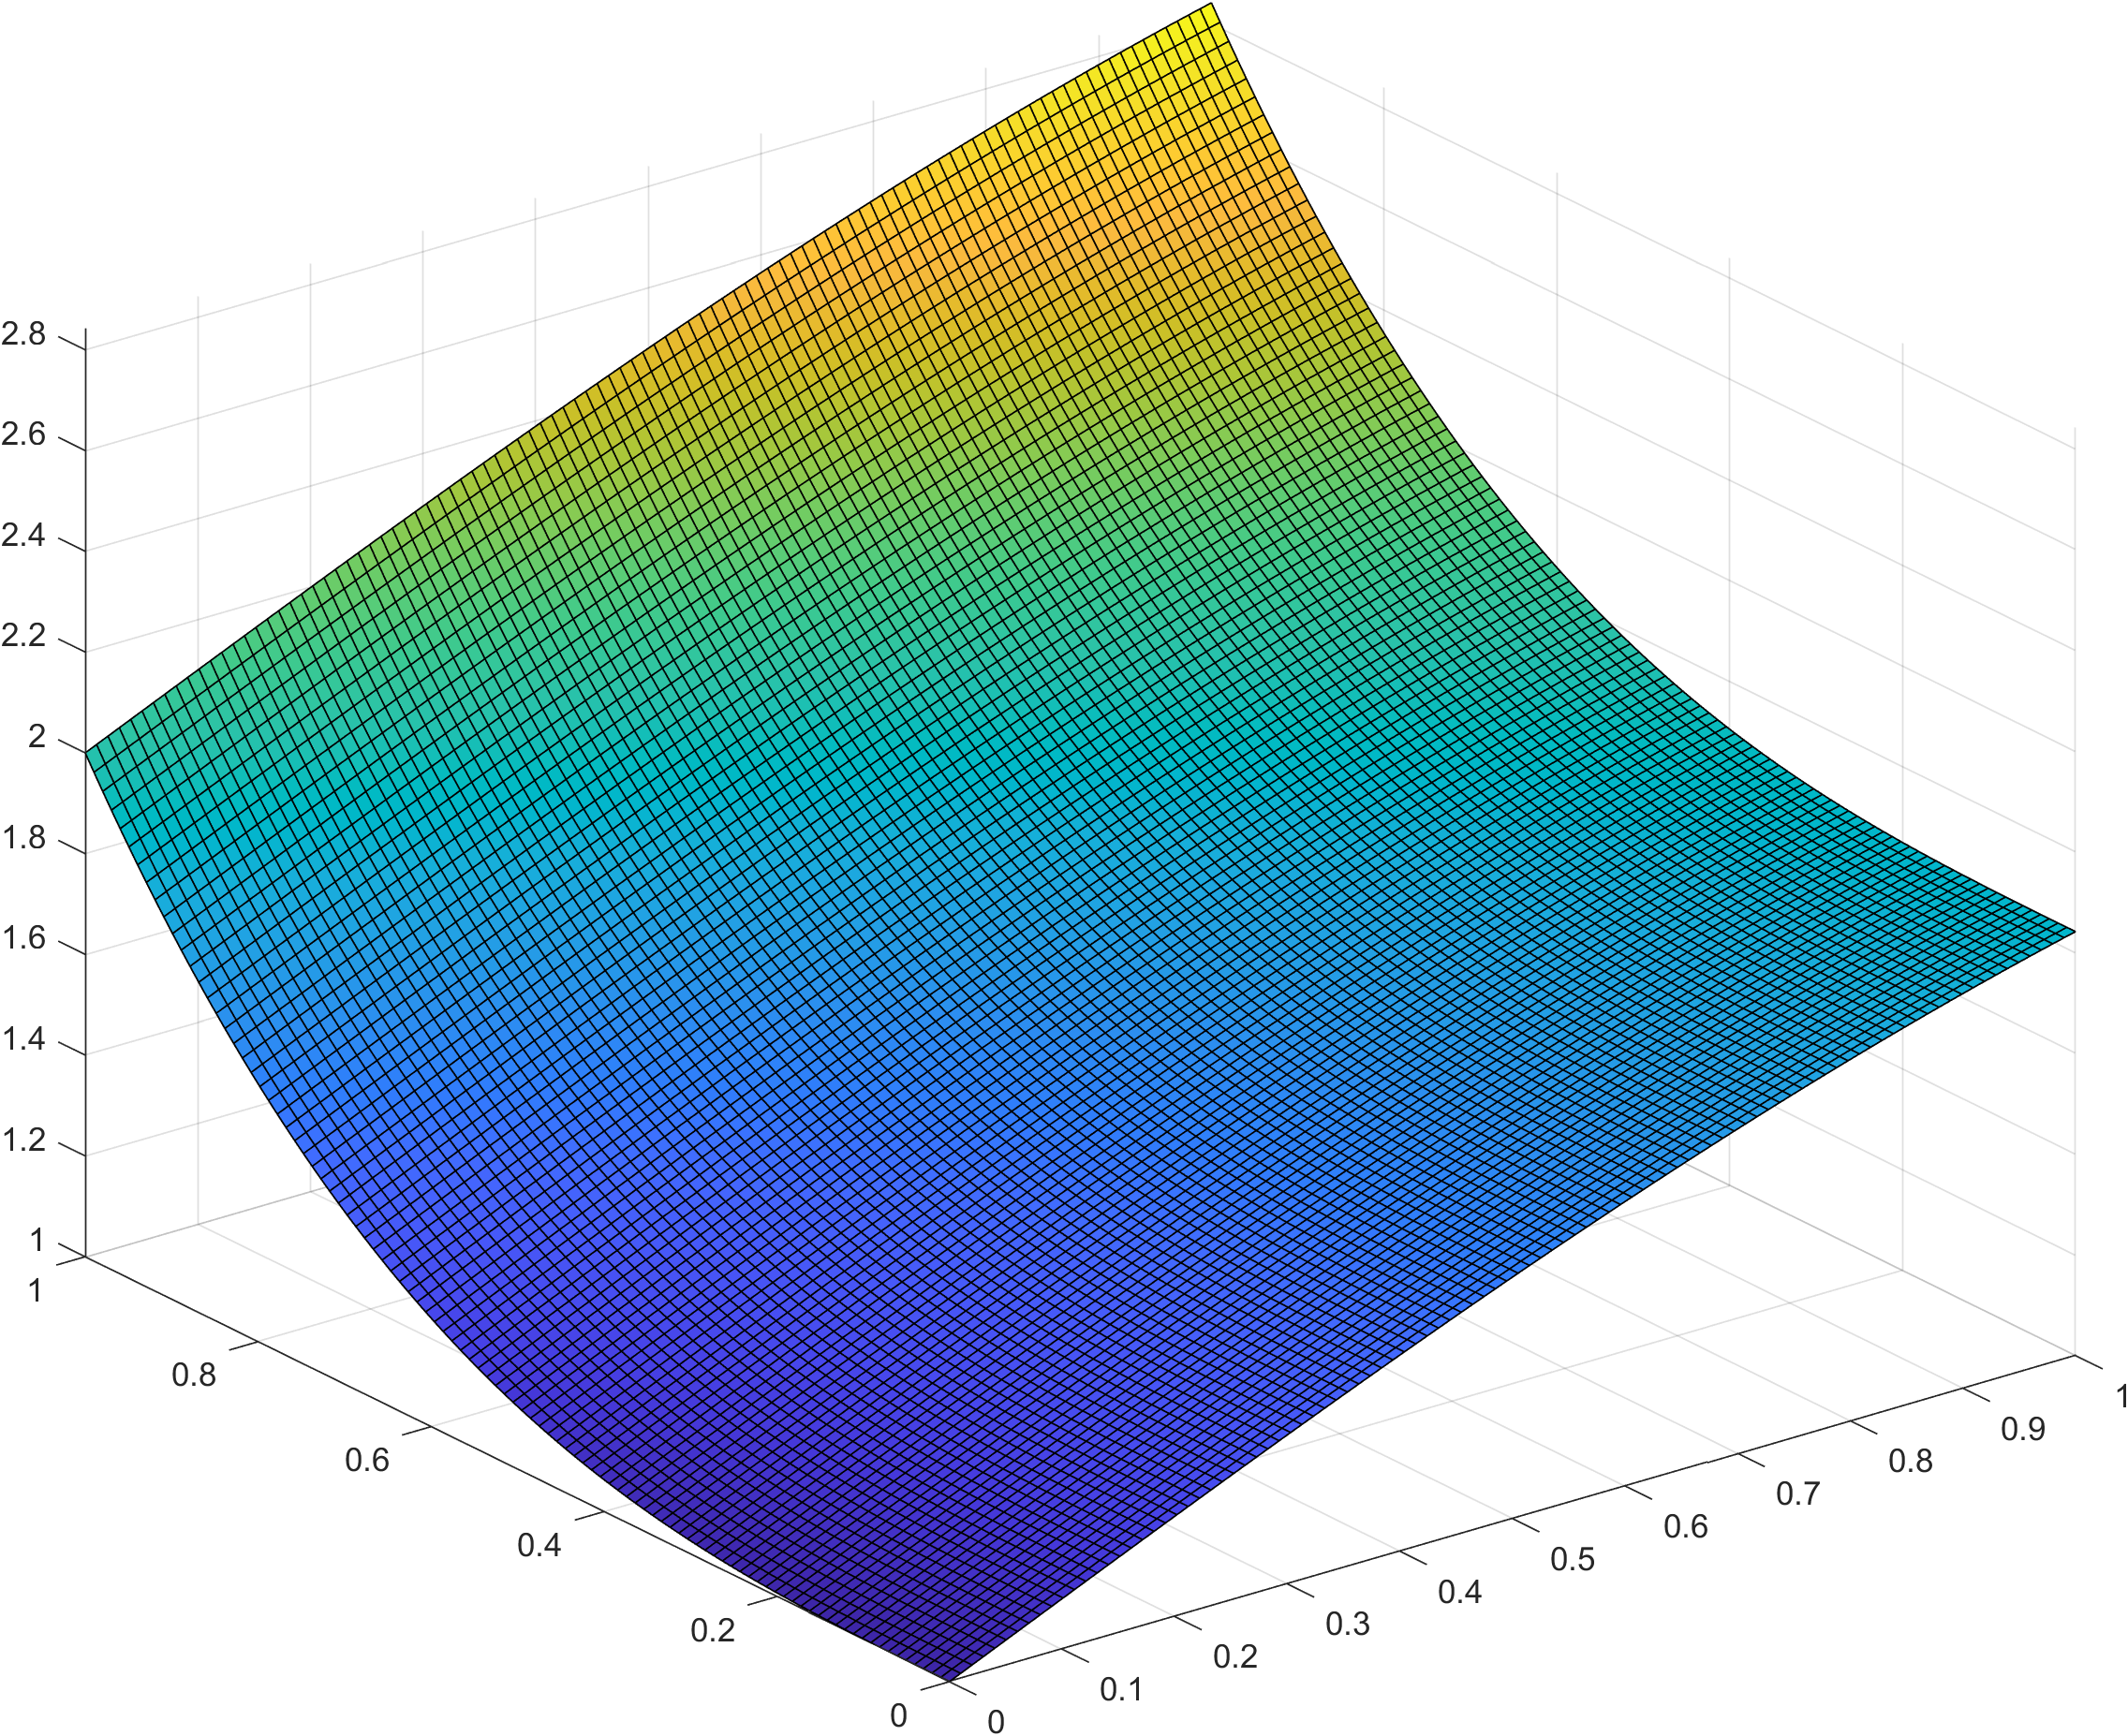
\includegraphics[height=\dimIm]{../Immagini/ES12_SE_NPunti=100_t=1.png}
                            \caption{Soluzione esatta al tempo $t=1$.}
                            \label{figES2TriangolazioniEsattaTF}
                        \end{subfigure}
                    }
                    \distR
                    
                    % \renewcommand{\dimIm}{4cm}
                    \makebox[\linewidth][c]{
                        \captionsetup[subfigure]{width=2.9cm}
                        \SpaziaturaMate{1}{1}{1}
                        \begin{subfigure}[t]{\lungSF}
                            \centering
                            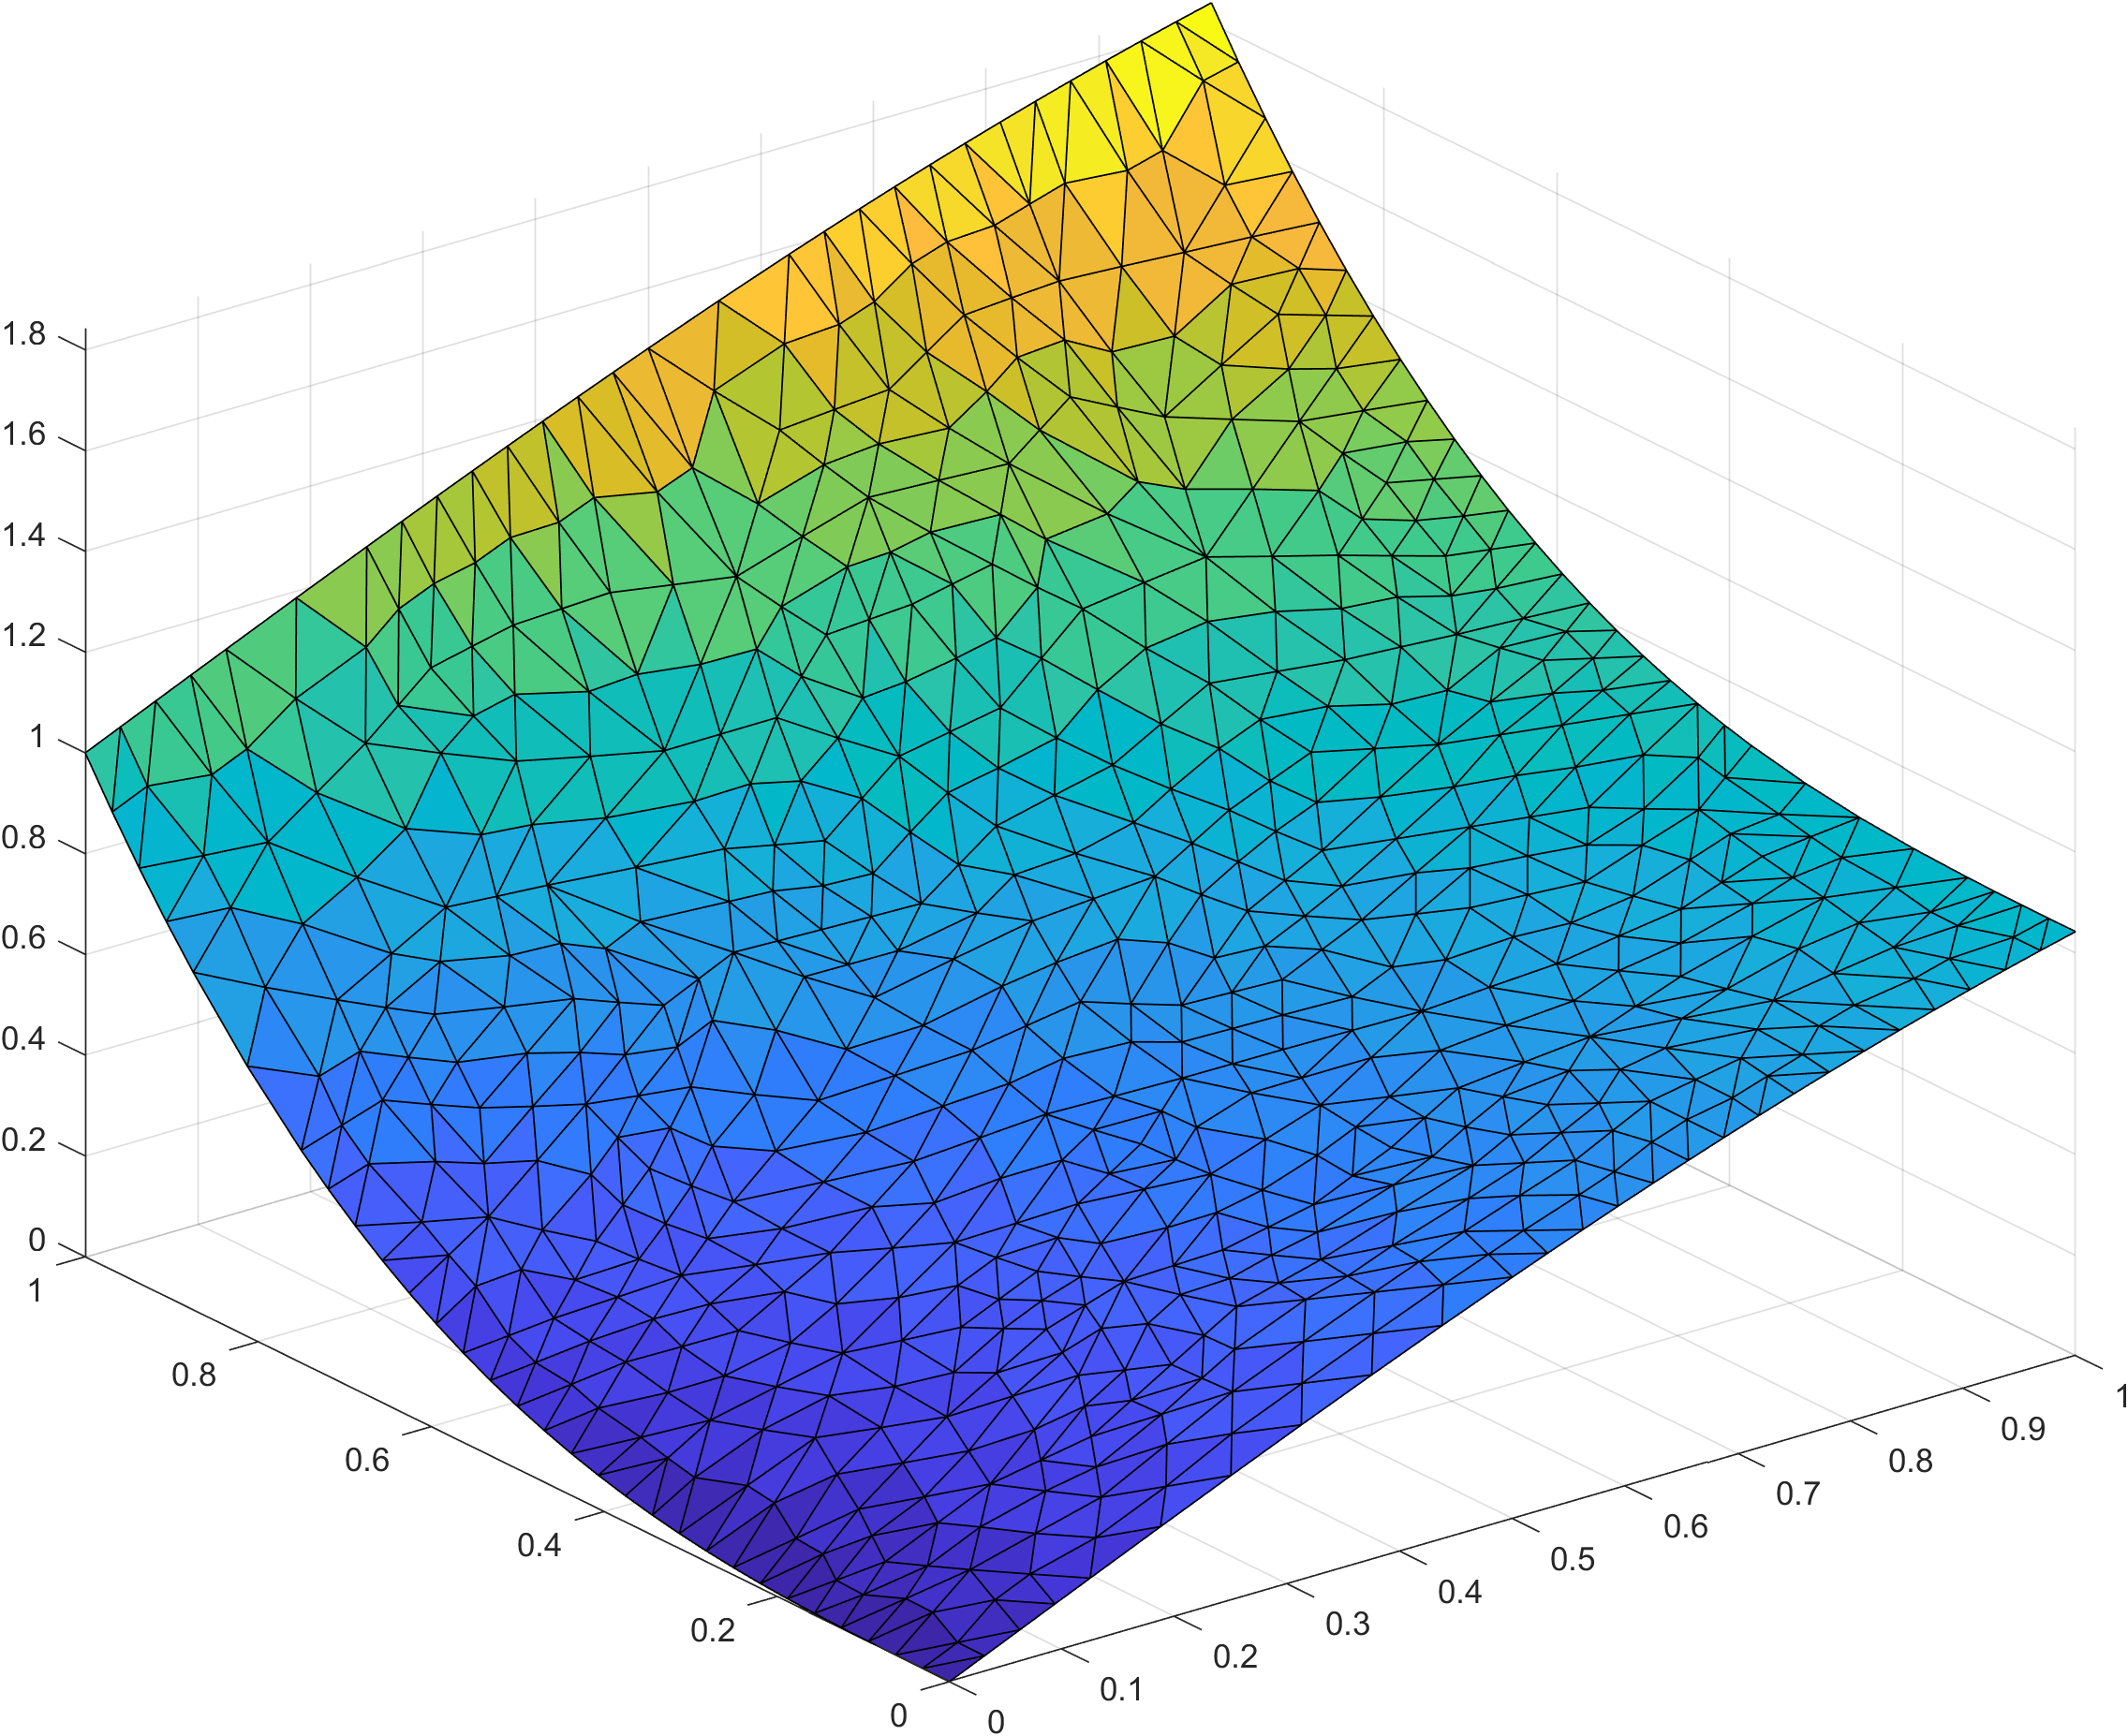
\includegraphics[height=\dimIm]{../Immagini/ES2_P2_AMax=dt=0.005_t=0.png}
                            \caption{Soluzione qualitativa coi $\mathbb{P}_2$ al tempo $t=0$.}
                            \label{figES2TriangolazioniP2TI}
                        \end{subfigure}
                        \begin{subfigure}[t]{\lungSF}
                            \centering
                            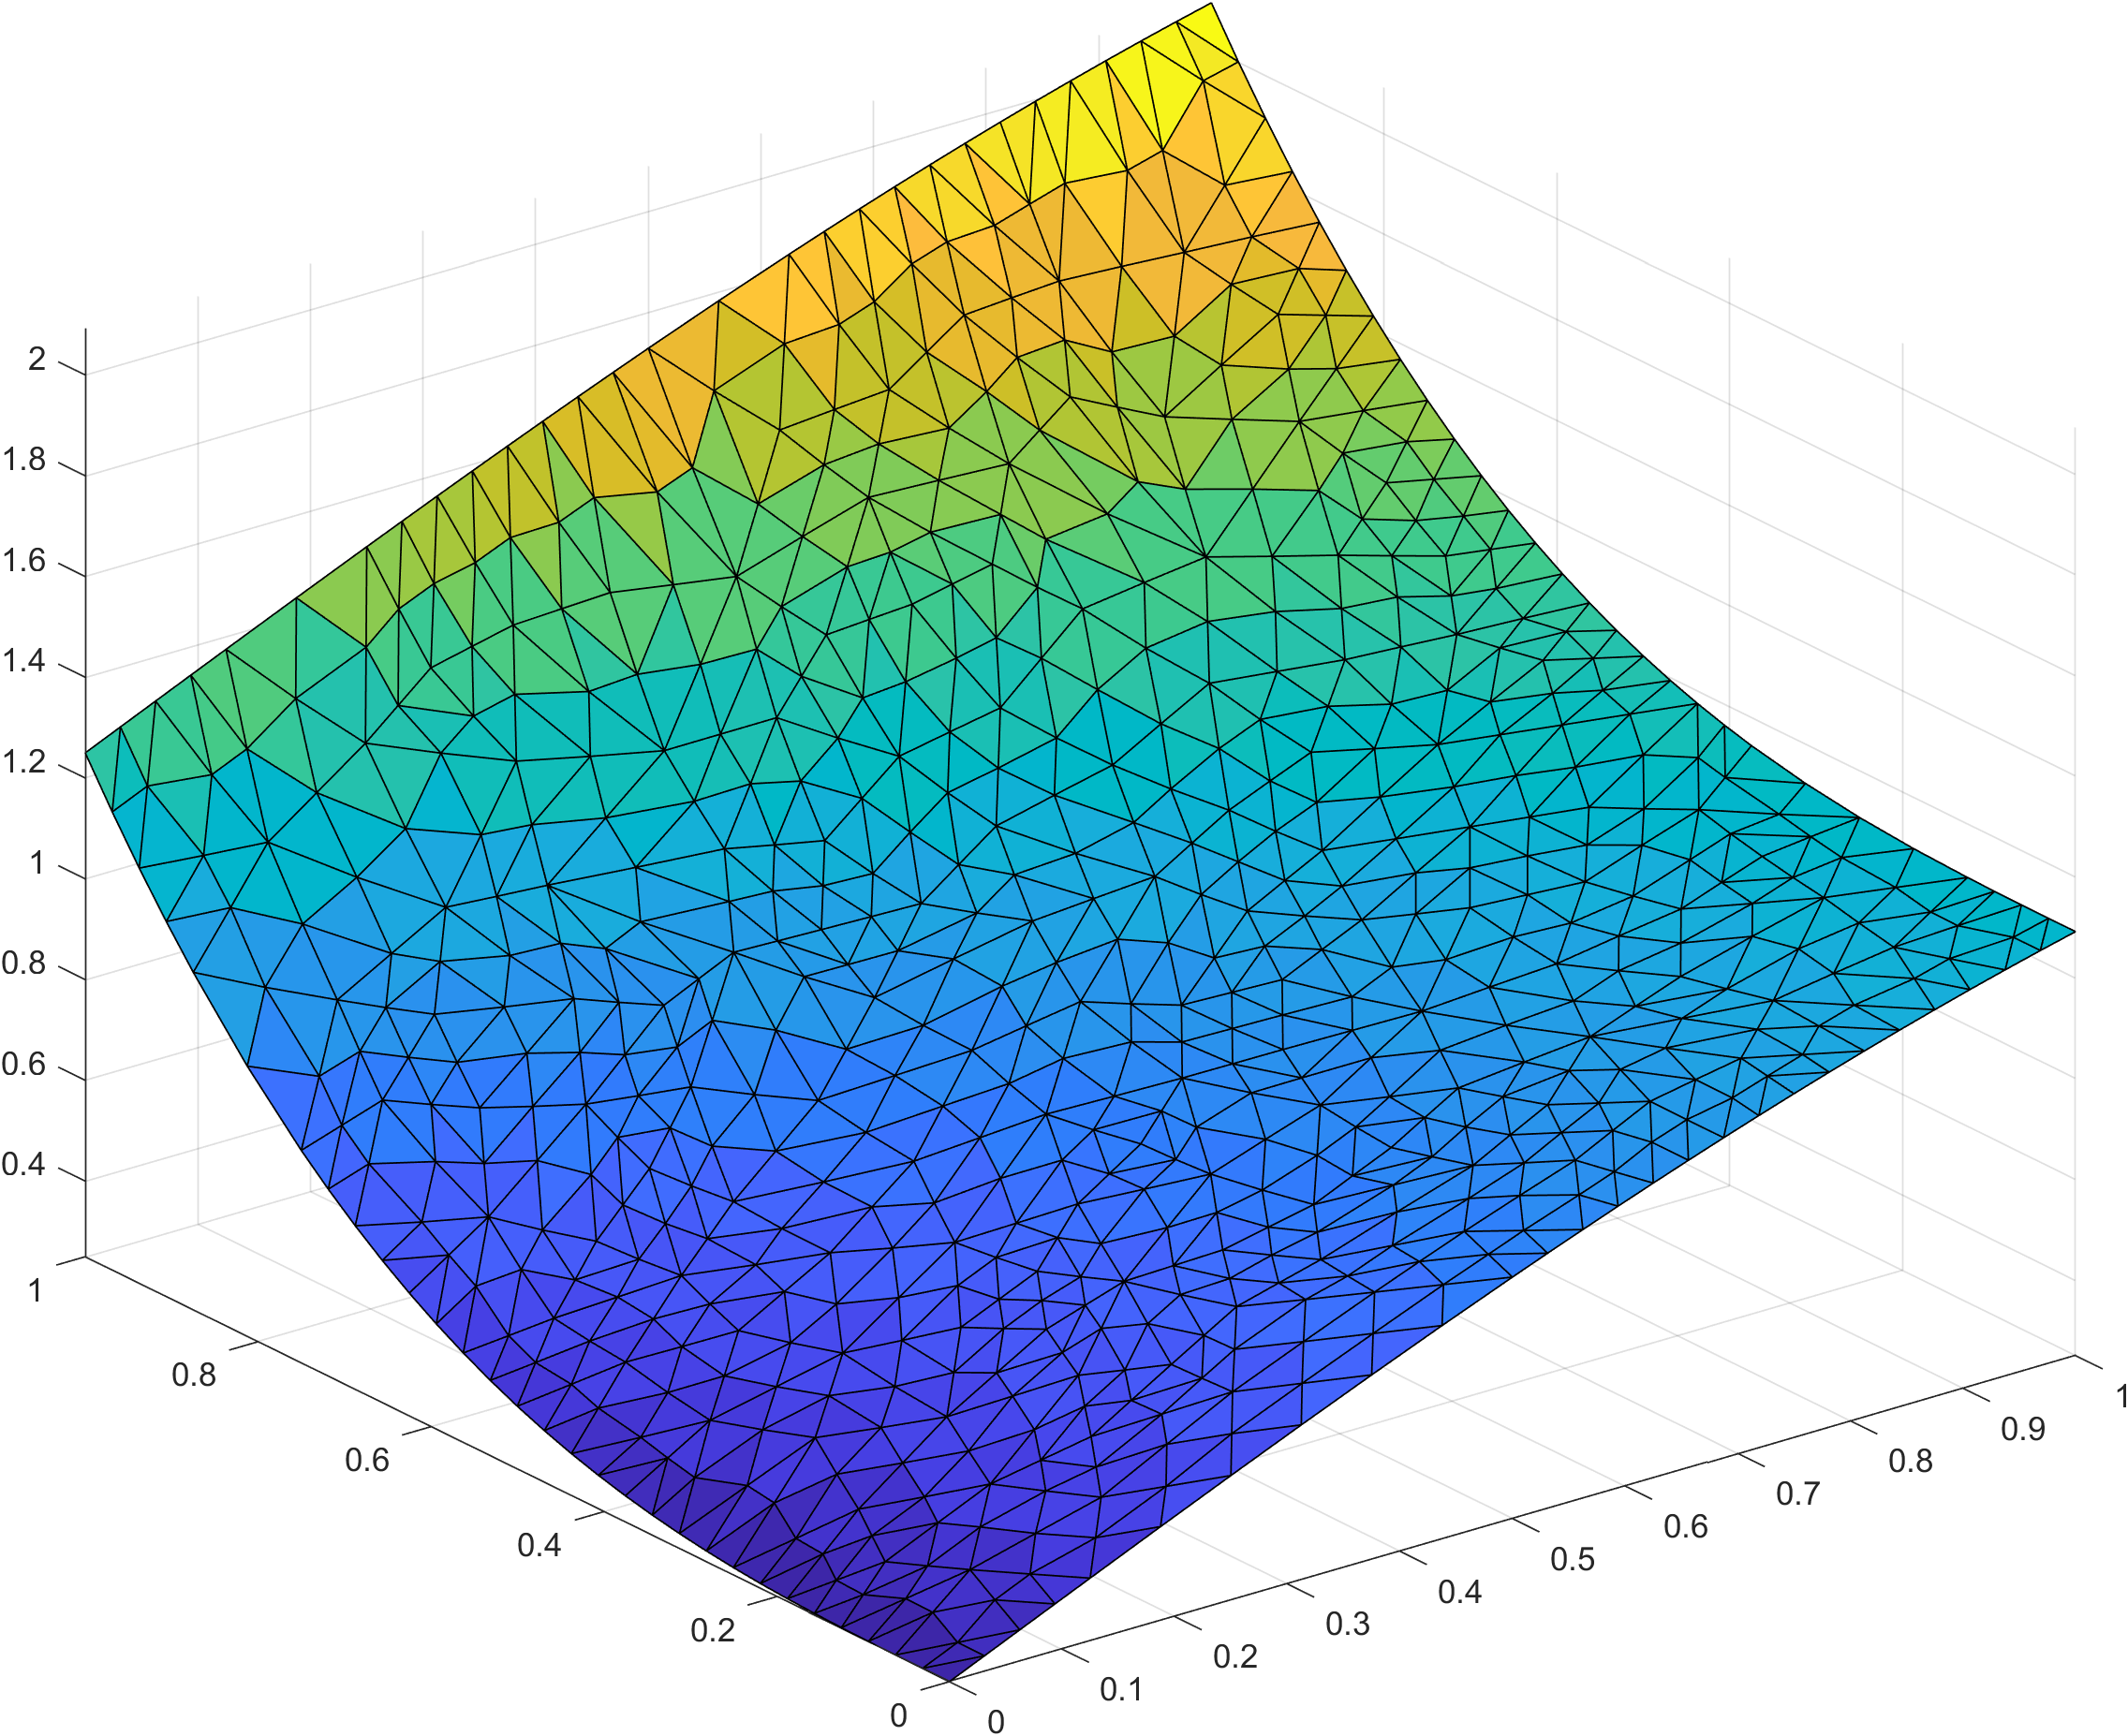
\includegraphics[height=\dimIm]{../Immagini/ES2_P2_AMax=dt=0.005_t=0.5.png}
                            \caption{Soluzione qualitativa coi $\mathbb{P}_2$ al tempo $t=0.5$.}
                            \label{figES2TriangolazioniP2TM}
                        \end{subfigure}
                        \begin{subfigure}[t]{\lungSF}
                            \centering
                            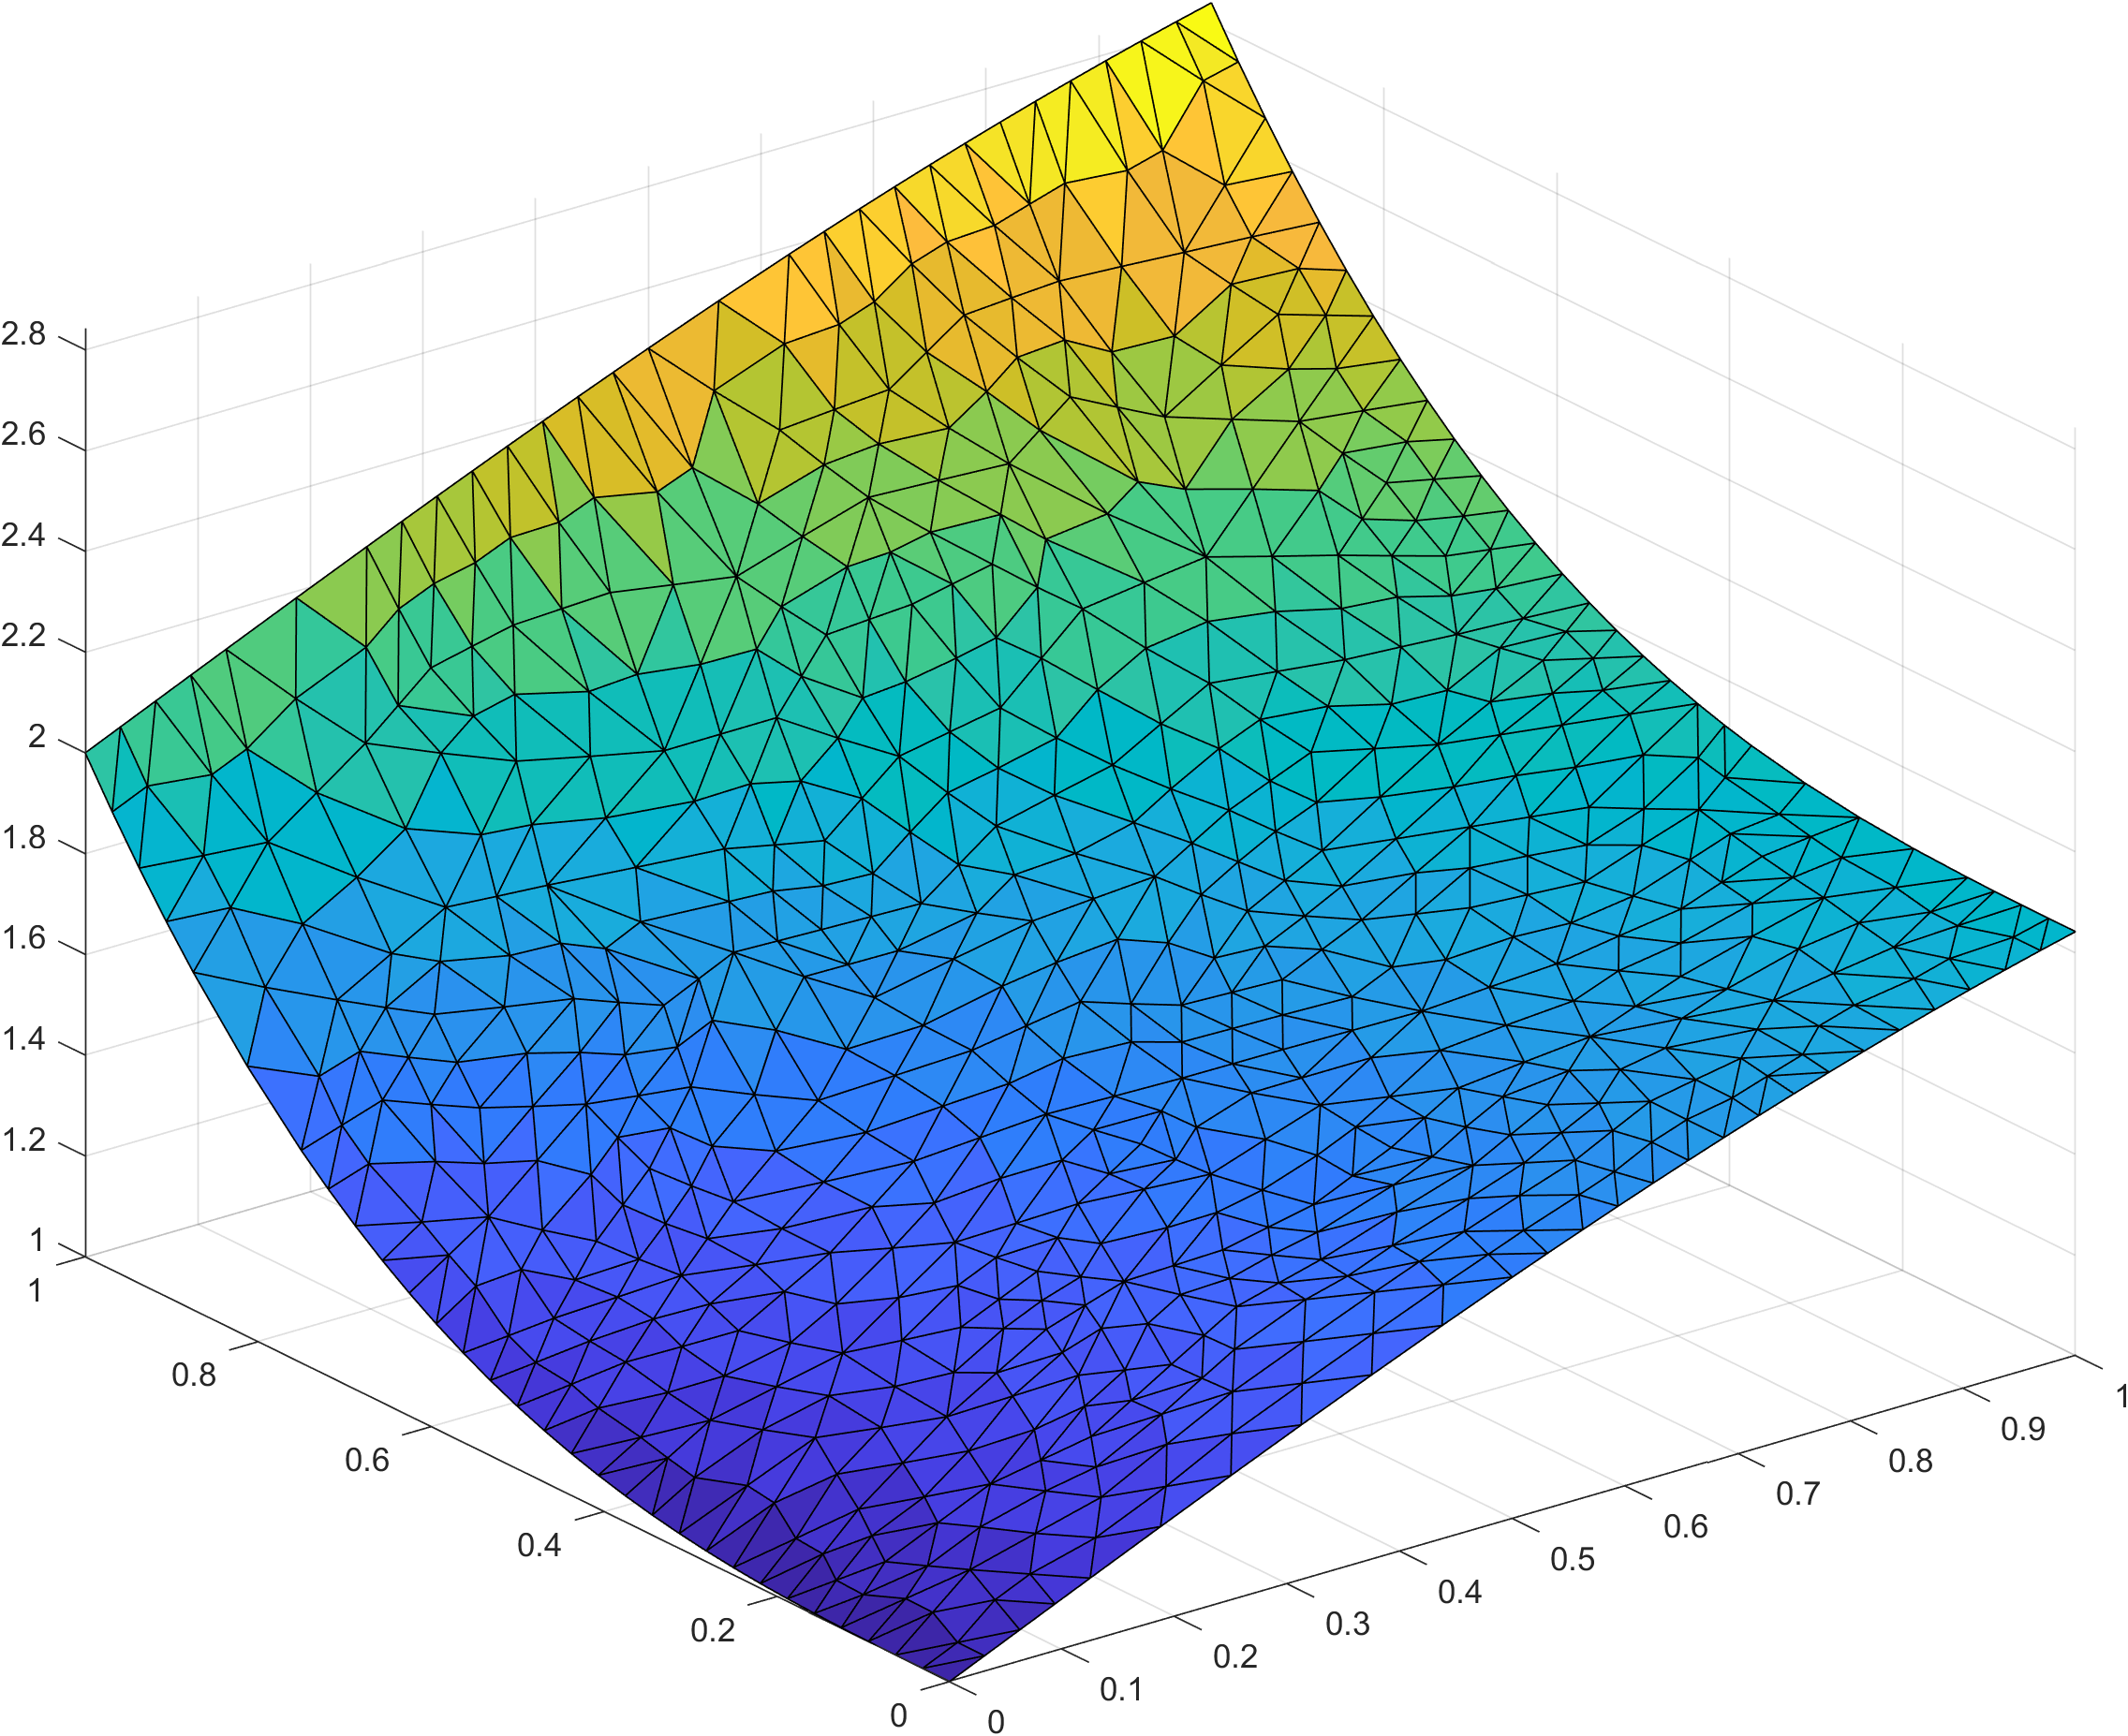
\includegraphics[height=\dimIm]{../Immagini/ES2_P2_AMax=dt=0.005_t=1.png}
                            \caption{Soluzione qualitativa coi $\mathbb{P}_2$ al tempo $t=1$.}
                            \label{figES2TriangolazioniP2TF}
                        \end{subfigure}
                    }
                    \distR
        
                    \renewcommand{\lungSF}{.5\linewidth}
                    \renewcommand{\dimIm}{\linewidth}
                    \newcommand{\distC}{\hspace{7.5pt}} % Distanza tra le colonne
                    \makebox[\linewidth][c]{
                        \begin{subfigure}[c]{\lungSF}
                            \centering
                            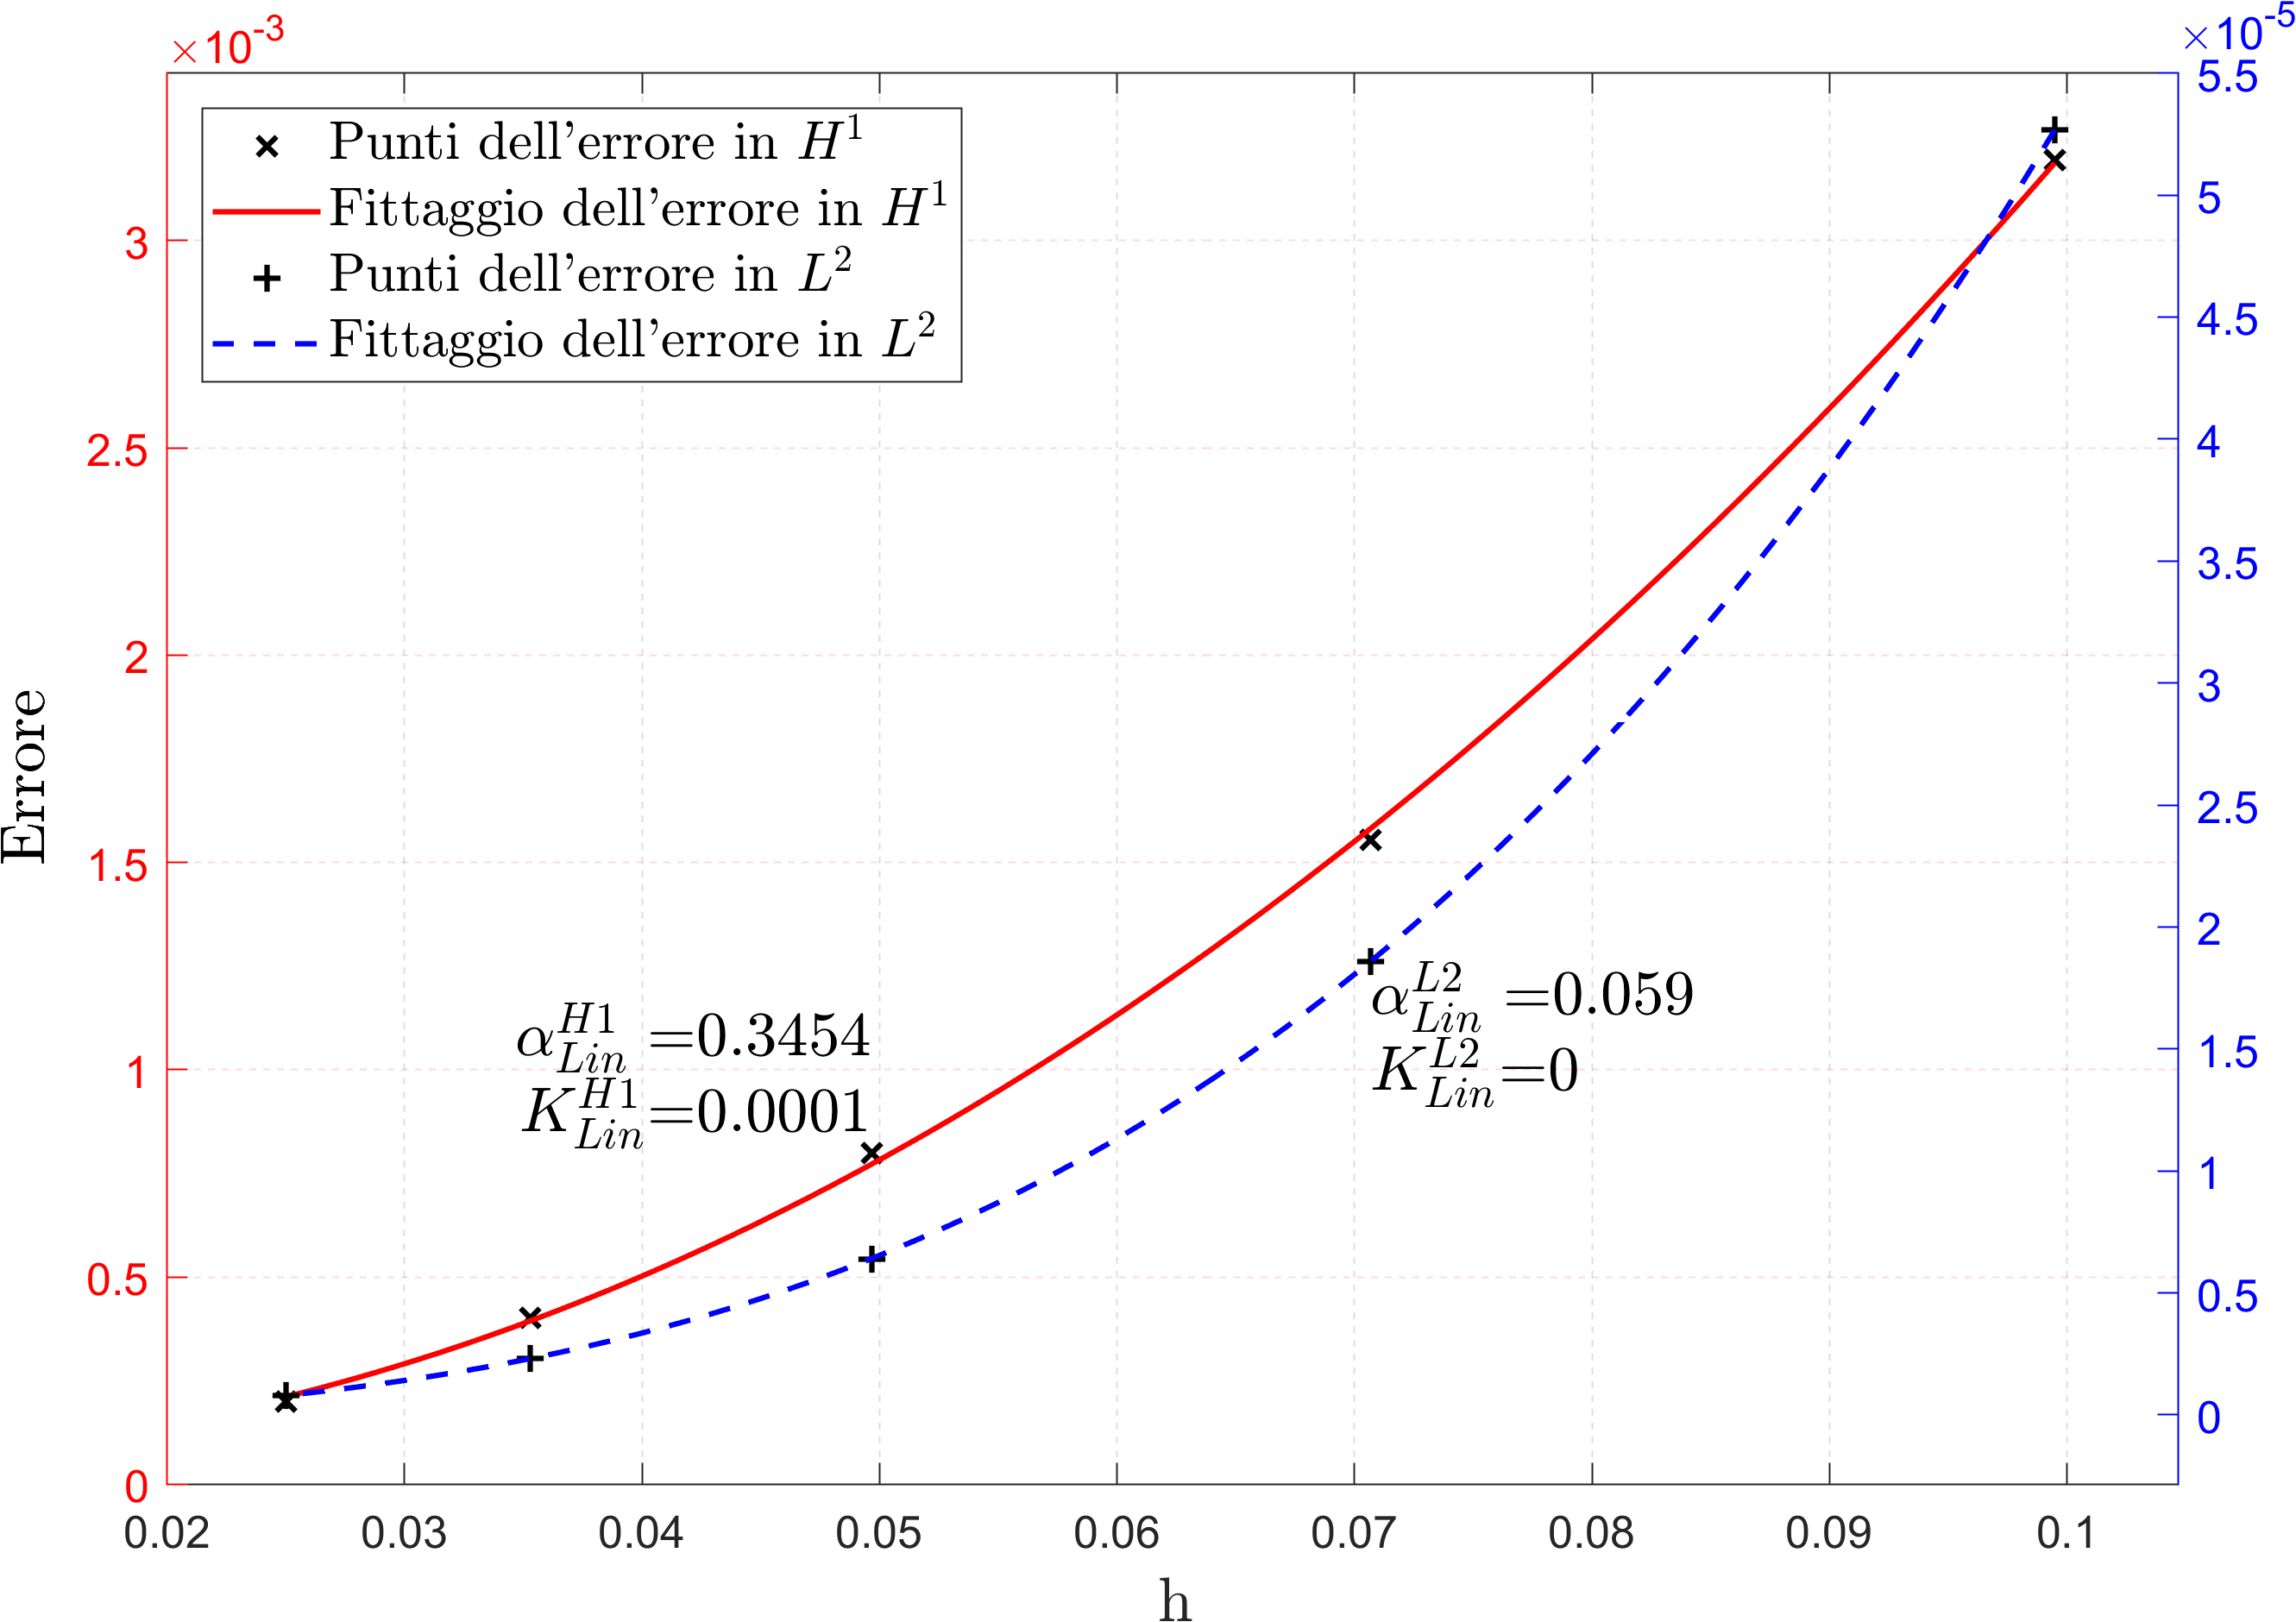
\includegraphics[width=\dimIm]{../Immagini/ES2_P2_ErrLin_AMax=dt=0.01_NSim=5.png}
                        \caption{Errore dei $\mathbb{P}_2$ in scala lineare.}
                        \label{figES2ErroreP2Lin}
                        \end{subfigure}
                        \distC
                        \begin{subfigure}[c]{\lungSF}
                            \centering
                            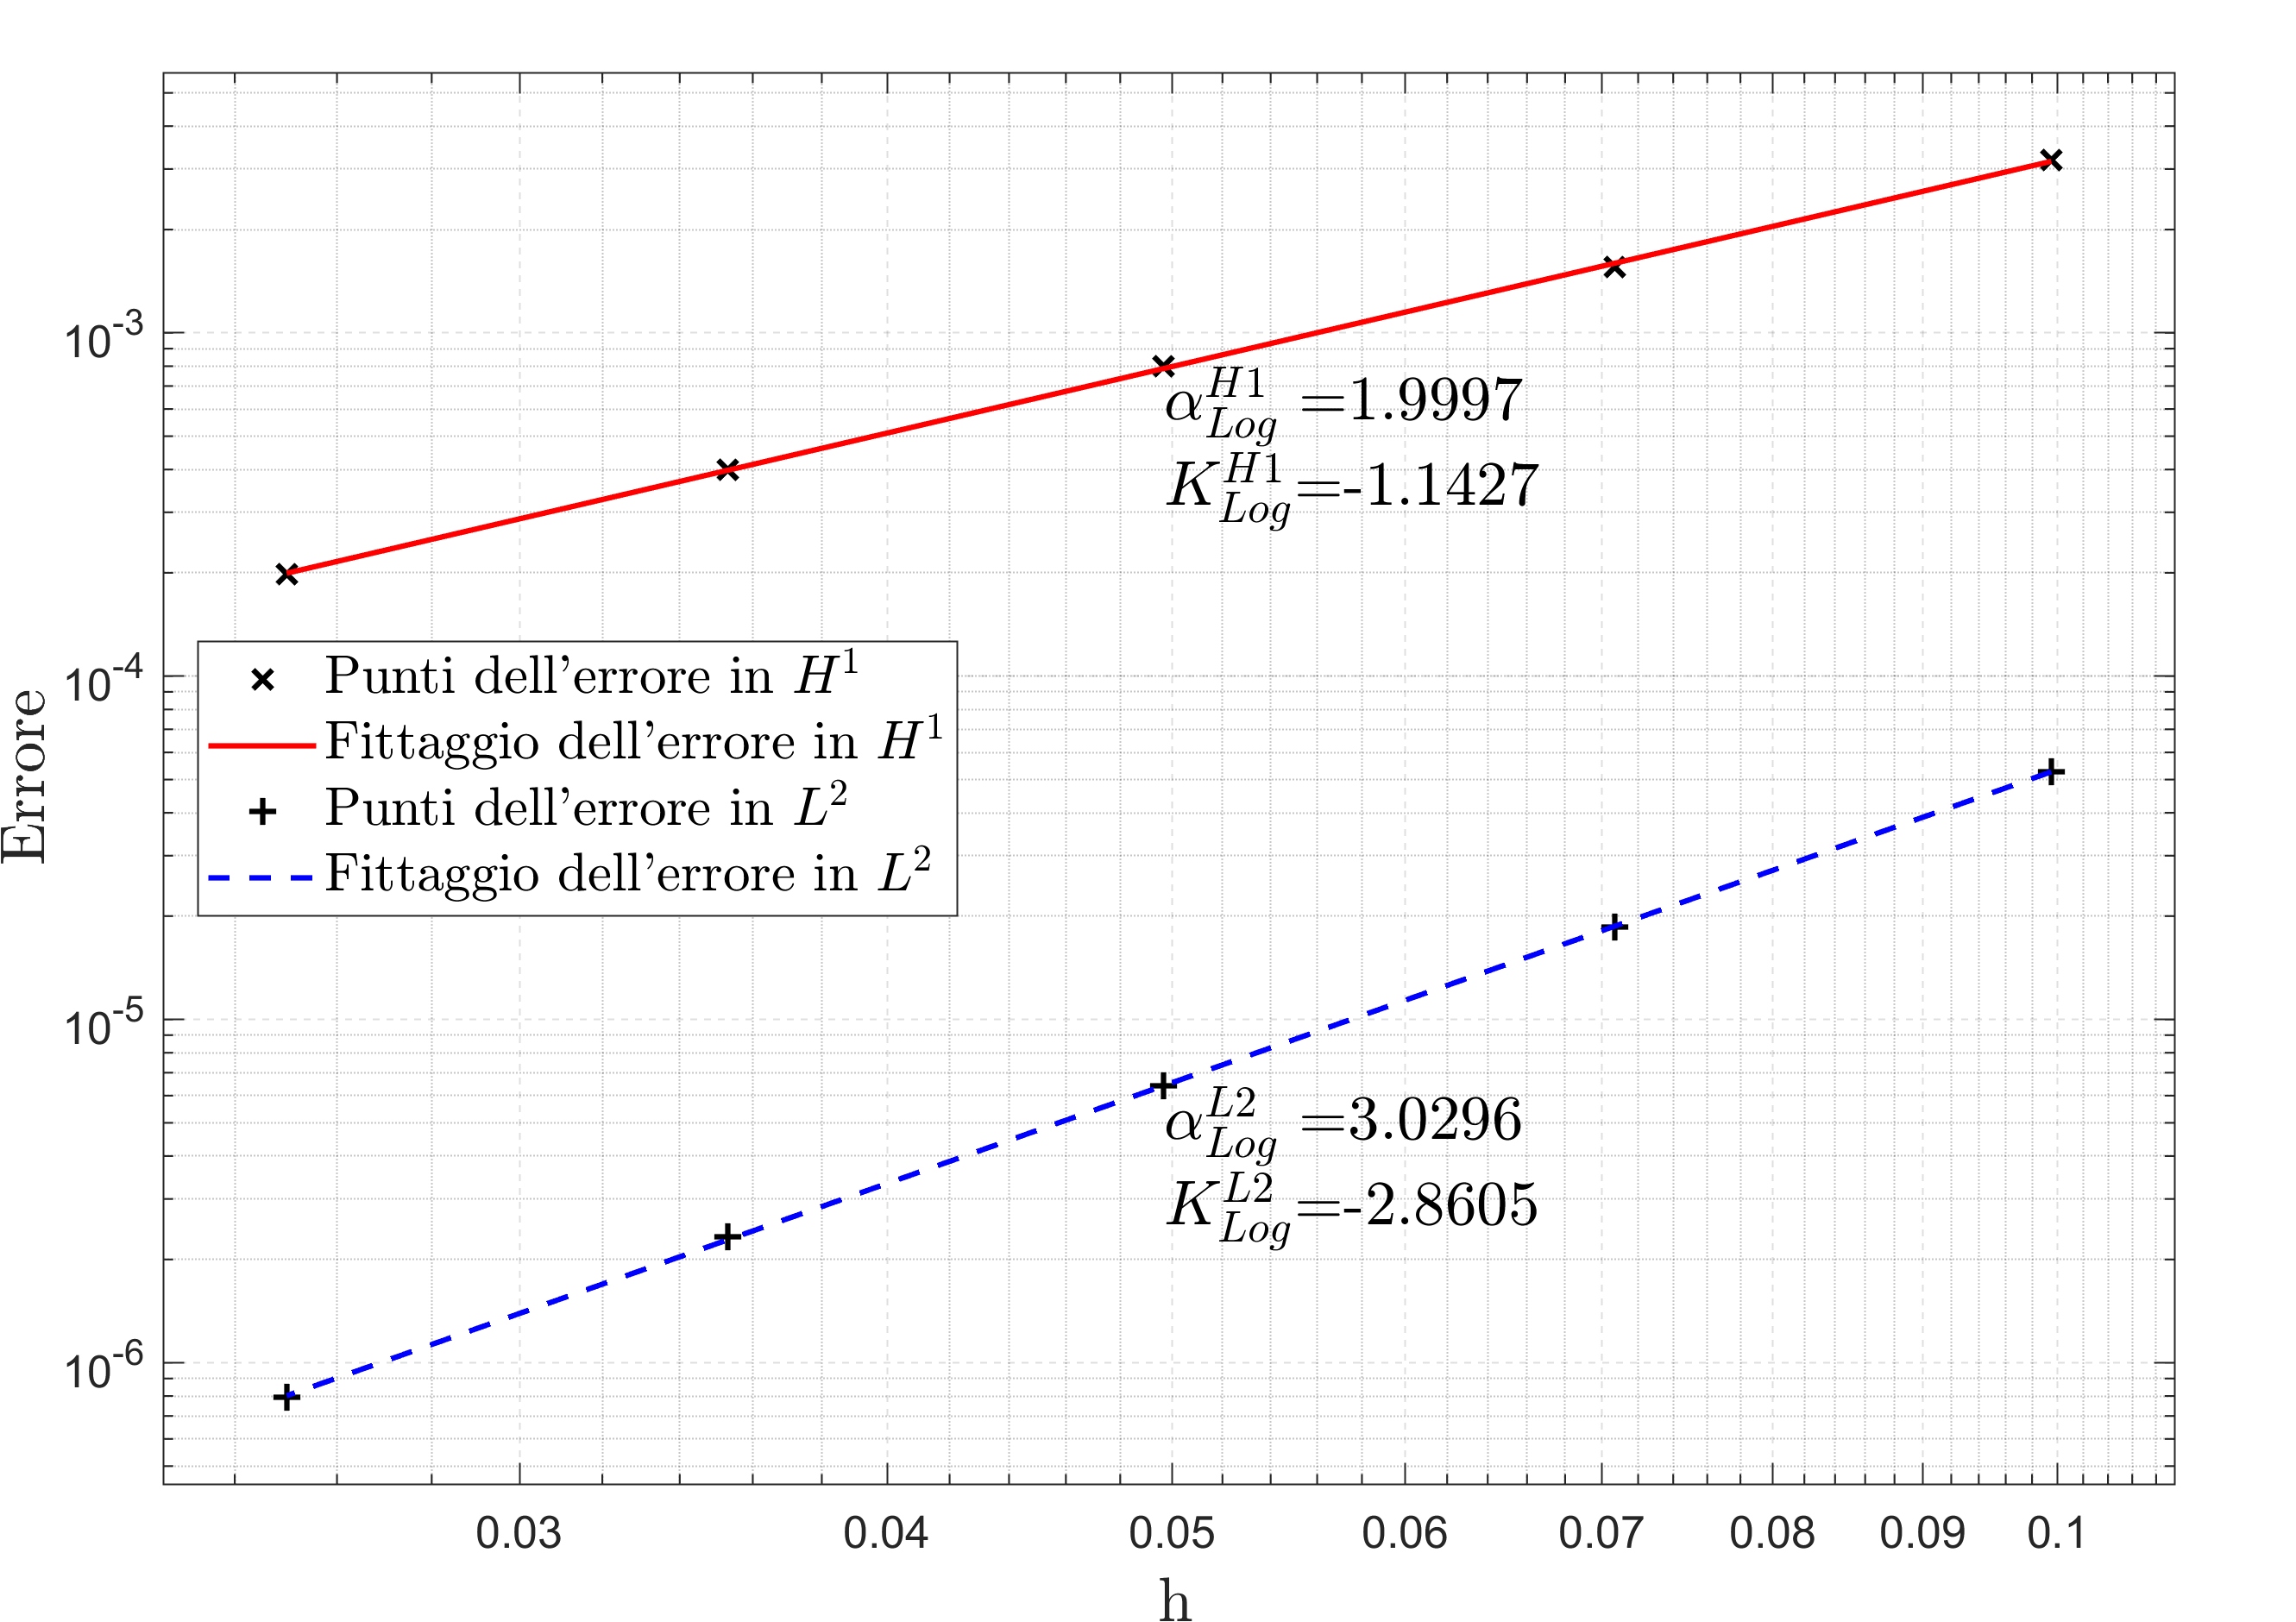
\includegraphics[width=\dimIm]{../Immagini/ES2_P2_ErrLog_AMax=dt=0.01_NSim=5.png}
                        \caption{Errore dei $\mathbb{P}_2$ in scala logaritmica.}
                        \label{figES2ErroreP2Log}
                        \end{subfigure}
                    }
                    \caption{Nelle Figg. \ref{figES2TriangolazioniEsattaTI}-\ref{figES2TriangolazioniP2TF} sono mostrate le soluzioni dell'ES2 in tre istanti temporali: le prime tre mostrano la soluzione esatta e le restanti quella approssimata; invece nelle \ref{figES2ErroreP2Lin} e \ref{figES2ErroreP2Log} sono illustrati in due scale diverse gli errori in norma $H^1$ ed $L^2$. I parametri dati a \textit{BBTR} sono spiegati nel $\S$\ref{parPremessaParametriBBTR}.}
                    \label{figES2}
                \end{figure*}
                %%%%%%%%%%%%%%%%%%
                %%%%%%%%%%%%%%%%%%
                %%%%%%%%%%%%%%%%%%

                %%%%%%%%%%%%%%%%%%%%%%%%%%%%
                %%% Tabella degli errori %%%
                %%%%%%%%%%%%%%%%%%%%%%%%%%%%
                {
                \setlength{\belowcaptionskip}{-0.3cm}
                \begin{table*}[p]
                    \centering
                    
                    % Spaziatura globale
                    \newcommand{\lunST}{0.49\textwidth} % Lunghezza sottotabella
                    \newcommand{\sepTabC}{\hspace{0.5cm}}  % Separazione delle tabelle
                    \newcommand{\sepTabR}{\vspace{0.3cm}}  % Separazione delle tabelle
                    
                    % Spaziatura locale
                    \newcommand{\sepCol}{\hspace{5pt}}
                    \newcommand{\lungTst}{0.5cm}
                    \renewcommand{\arraystretch}{1.5}
                    
                    \makebox[\textwidth][c]{
                        \begin{subtable}[t]{\lunST}
                            \centering
                            \begin{tabular}{c@{}|@{\sepCol}c@{\sepCol}c@{\sepCol}c@{\sepCol}c@{\sepCol}c}
                                $\Delta t$&
                                \notaSci{1.00}{-2}&
                                \notaSci{5.00}{-3}&
                                \notaSci{2.50}{-3}&
                                \notaSci{1.25}{-3}&
                                \notaSci{6.25}{-4}\\
                                \hline
                                $\text{err}_{L^2}^{\mathbb P_1}$&
                                \notaSci{2.45}{-6}&
                                \notaSci{6.13}{-7}&
                                \notaSci{1.53}{-7}&
                                \notaSci{3.83}{-8}&
                                \notaSci{9.57}{-9}\\
                                $\text{err}_{H^1}^{\mathbb P_1}$&
                                \notaSci{1.44}{-5}&
                                \notaSci{3.59}{-6}&
                                \notaSci{8.98}{-7}&
                                \notaSci{2.24}{-7}&
                                \notaSci{5.61}{-8}
                            \end{tabular}
                            \caption{ET1.\sepTabR}
                            \label{tabErroriET1}
                        \end{subtable}
                        \sepTabC
                        \begin{subtable}[t]{\lunST}
                            \centering
                            \begin{tabular}{c@{}|@{\sepCol}c@{\sepCol}c@{\sepCol}c@{\sepCol}c@{\sepCol}c}
                                $\Delta t$&
                                \notaSci{1.00}{-2}&
                                \notaSci{5.00}{-3}&
                                \notaSci{2.50}{-3}&
                                \notaSci{1.25}{-3}&
                                \notaSci{6.25}{-4}\\
                                \hline
                                $\text{err}_{L^2}^{\mathbb P_2}$&
                                \notaSci{2.38}{-6}&
                                \notaSci{5.94}{-7}&
                                \notaSci{1.49}{-7}&
                                \notaSci{3.71}{-8}&
                                \notaSci{9.29}{-9}\\
                                $\text{err}_{H^1}^{\mathbb P_2}$&
                                \notaSci{1.46}{-5}&
                                \notaSci{3.64}{-6}&
                                \notaSci{9.10}{-7}&
                                \notaSci{2.28}{-7}&
                                \notaSci{5.69}{-8}
                            \end{tabular}
                            \caption{ET2.\sepTabR}
                            \label{tabErroriET2}
                        \end{subtable}
                    }
                    \makebox[\textwidth][c]{
                        \begin{subtable}[t]{\lunST}
                            \centering
                            \begin{tabular}{c@{}|@{\sepCol}c@{\sepCol}c@{\sepCol}c@{\sepCol}c@{\sepCol}c}
                                $h$&
                                \notaSci{9.95}{-2}&
                                \notaSci{7.07}{-2}&
                                \notaSci{4.97}{-2}&
                                \notaSci{3.53}{-2}&
                                \notaSci{2.50}{-2}\\
                                \hline
                                $\text{err}_{L^2}^{\mathbb P_1}$&
                                    \notaSci{4.24}{-3}&
                                    \notaSci{1.84}{-3}&
                                    \notaSci{9.51}{-4}&
                                    \notaSci{4.74}{-4}&
                                    \notaSci{2.41}{-4}\\
                                $\text{err}_{H^1}^{\mathbb P_1}$&
                                    \notaSci{1.26}{-1}&
                                    \notaSci{8.68}{-2}&
                                    \notaSci{6.16}{-2}&
                                    \notaSci{4.30}{-2}&
                                    \notaSci{3.06}{-2}
                            \end{tabular}
                            \caption{ES1.}
                            \label{tabErroriES1}
                        \end{subtable}
                        \sepTabC
                        \begin{subtable}[t]{\lunST}
                            \centering
                            \begin{tabular}{c@{}|@{\sepCol}c@{\sepCol}c@{\sepCol}c@{\sepCol}c@{\sepCol}c}
                                $h$&
                                \notaSci{9.95}{-2}&
                                \notaSci{7.07}{-2}&
                                \notaSci{4.97}{-2}&
                                \notaSci{3.53}{-2}&
                                \notaSci{2.50}{-2}\\
                                \hline
                                $\text{err}_{L^2}^{\mathbb P_2}$&
                                    \notaSci{5.27}{-5}&
                                    \notaSci{1.86}{-5}&
                                    \notaSci{6.40}{-6}&
                                    \notaSci{2.33}{-6}&
                                    \notaSci{7.92}{-7}\\
                                $\text{err}_{H^1}^{\mathbb P_2}$&
                                    \notaSci{3.19}{-3}&
                                    \notaSci{1.55}{-3}&
                                    \notaSci{7.98}{-4}&
                                    \notaSci{4.00}{-4}&
                                    \notaSci{1.99}{-4}
                            \end{tabular}
                            \caption{ES2.}
                            \label{tabErroriES2}
                        \end{subtable}
                    }
                    \caption{Dati relativi all'errore nell'E.}
                    \label{tabErroriE}
                \end{table*}
                }
                %%%%%%%%%%%%%%%%%%%%%%%%%%%%
                %%%%%%%%%%%%%%%%%%%%%%%%%%%%
                %%%%%%%%%%%%%%%%%%%%%%%%%%%%

                %%%%%%%%%%%%%%%%%%%%%%%%
                %%% Infoimmagini EGM %%%
                %%%%%%%%%%%%%%%%%%%%%%%%
                \begin{figure*}[p]
                    \newcommand{\distR}{\vspace{0pt}} % Distanza tra le righe

                    \newcommand{\lungSF}{0.33\textwidth}
                    \newcommand{\dimIm}{4.4cm}

                    \makebox[\linewidth][c]{
                        % \captionsetup[subfigure]{width=2.4cm}
                        \SpaziaturaMate{1}{1}{1}
                        \begin{subfigure}[t]{\lungSF}
                            \centering
                            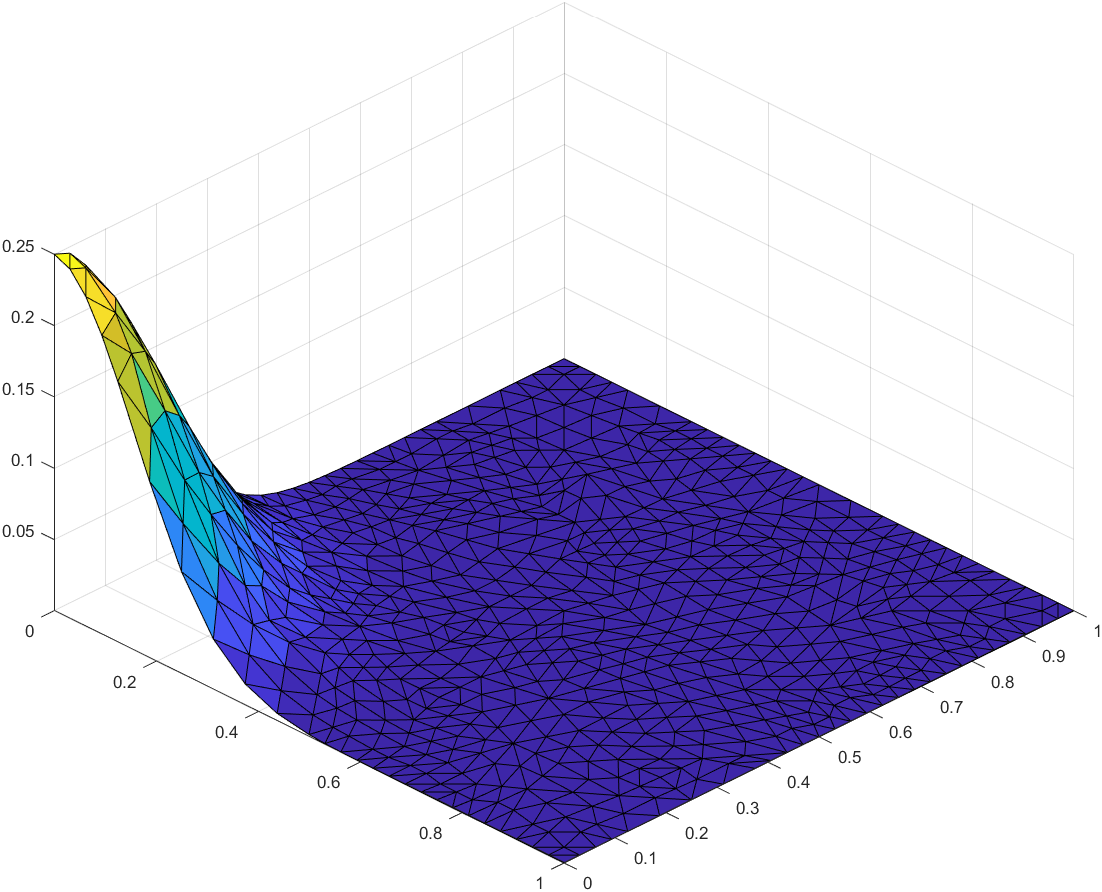
\includegraphics[height=\dimIm]{../Immagini/EGM_P2_AMax=dt=0.005_t=0.png}
                            \caption{Tempo $t=0$.}
                            \label{figEGMTriangolazioniT1}
                        \end{subfigure}
                        \begin{subfigure}[t]{\lungSF}
                            \centering
                            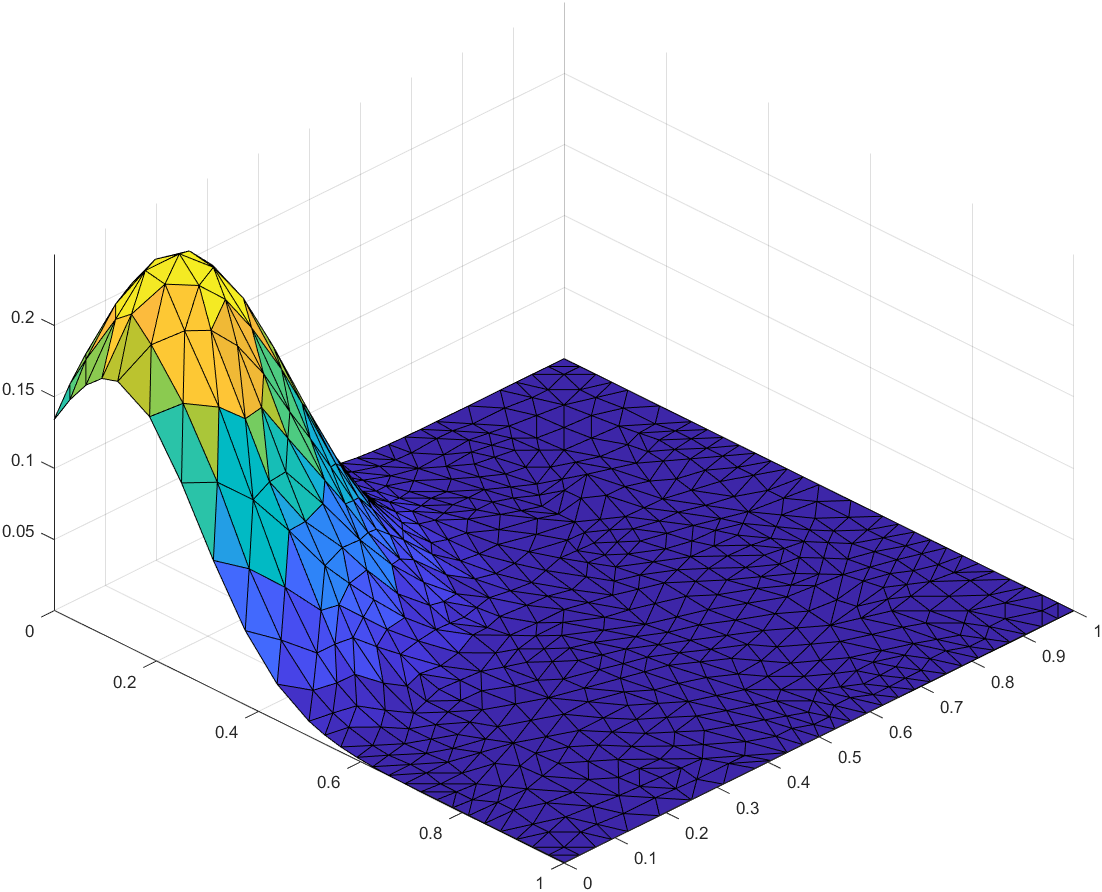
\includegraphics[height=\dimIm]{../Immagini/EGM_P2_AMax=dt=0.005_t=0.125.png}
                            \caption{Tempo $t=0.125$.}
                            \label{figEGMTriangolazioniT2}
                        \end{subfigure}
                        \begin{subfigure}[t]{\lungSF}
                            \centering
                            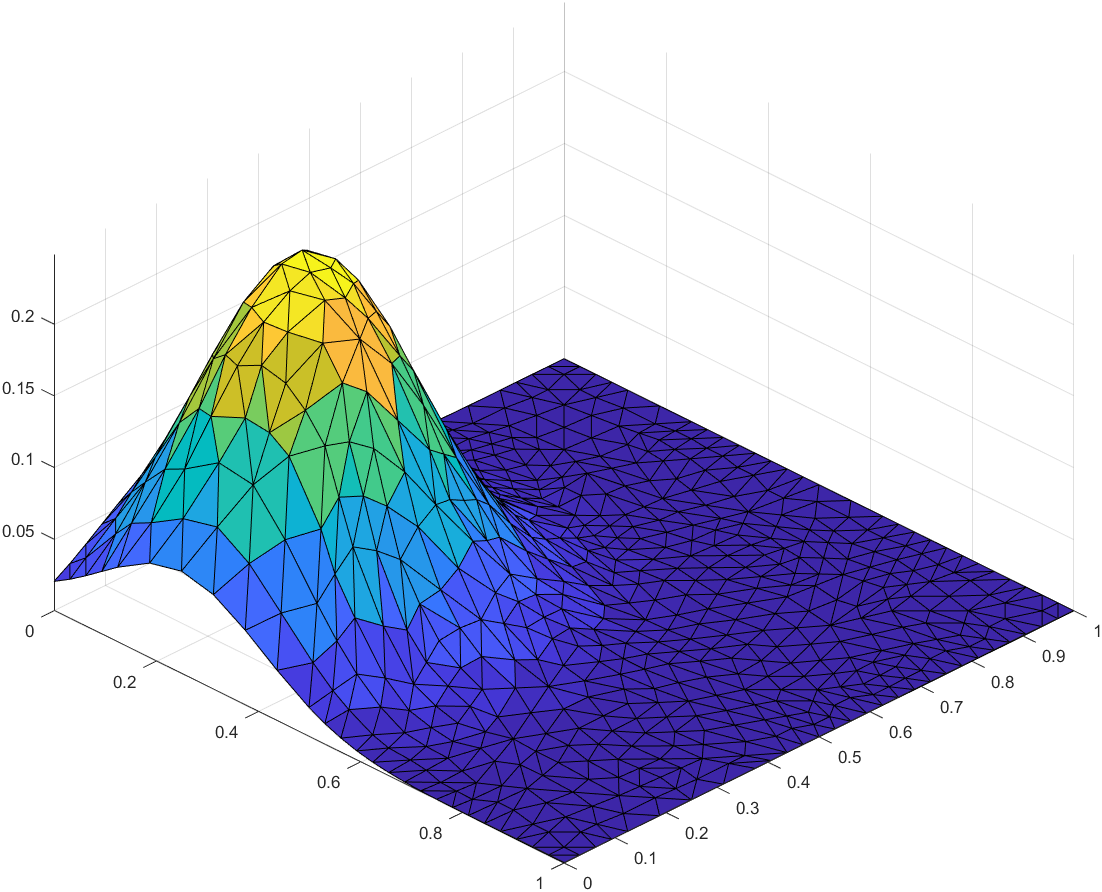
\includegraphics[height=\dimIm]{../Immagini/EGM_P2_AMax=dt=0.005_t=0.25.png}
                            \caption{Tempo $t=0.25$.}
                            \label{figEGMTriangolazioniT3}
                        \end{subfigure}
                    }
                    \distR
                    
                    \makebox[\linewidth][c]{
                        % \captionsetup[subfigure]{width=2.4cm}
                        \SpaziaturaMate{1}{1}{1}
                        \begin{subfigure}[t]{\lungSF}
                            \centering
                            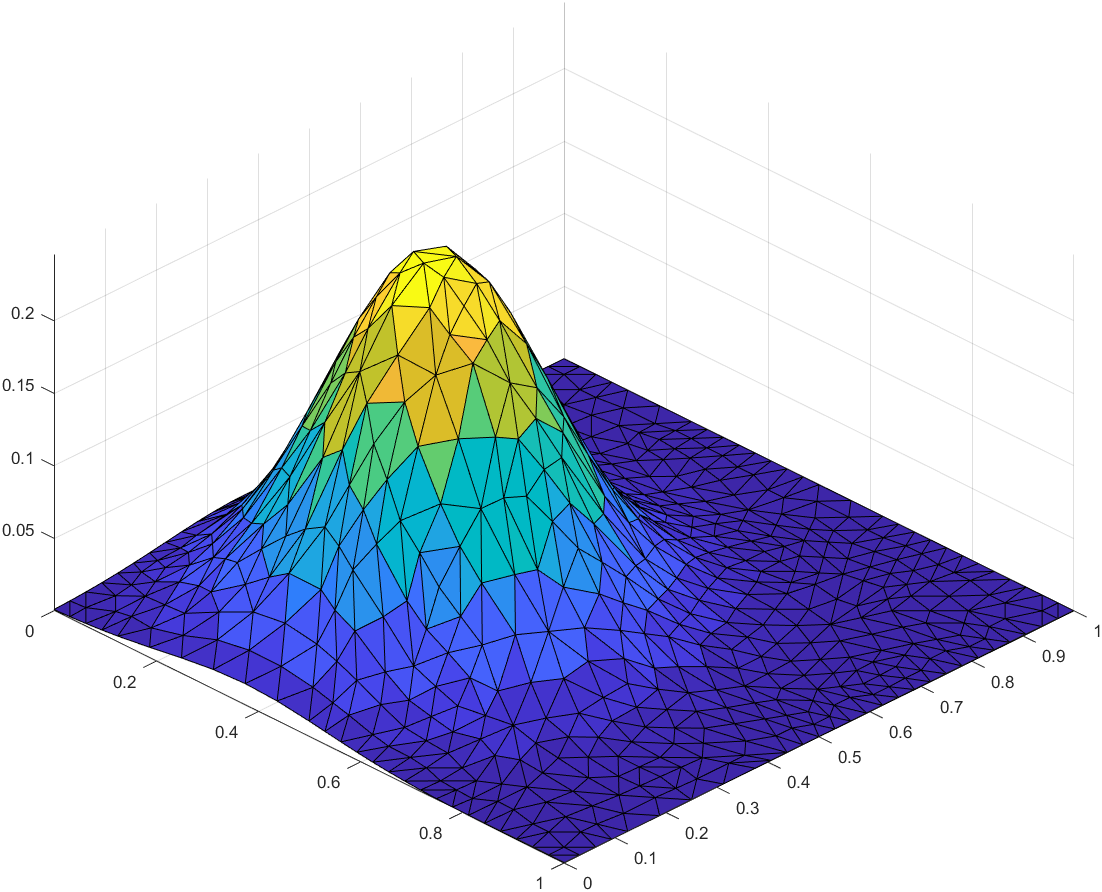
\includegraphics[height=\dimIm]{../Immagini/EGM_P2_AMax=dt=0.005_t=0.375.png}
                            \caption{Tempo $t=0.375$.}
                            \label{figEGMTriangolazioniT4}
                        \end{subfigure}
                        \begin{subfigure}[t]{\lungSF}
                            \centering
                            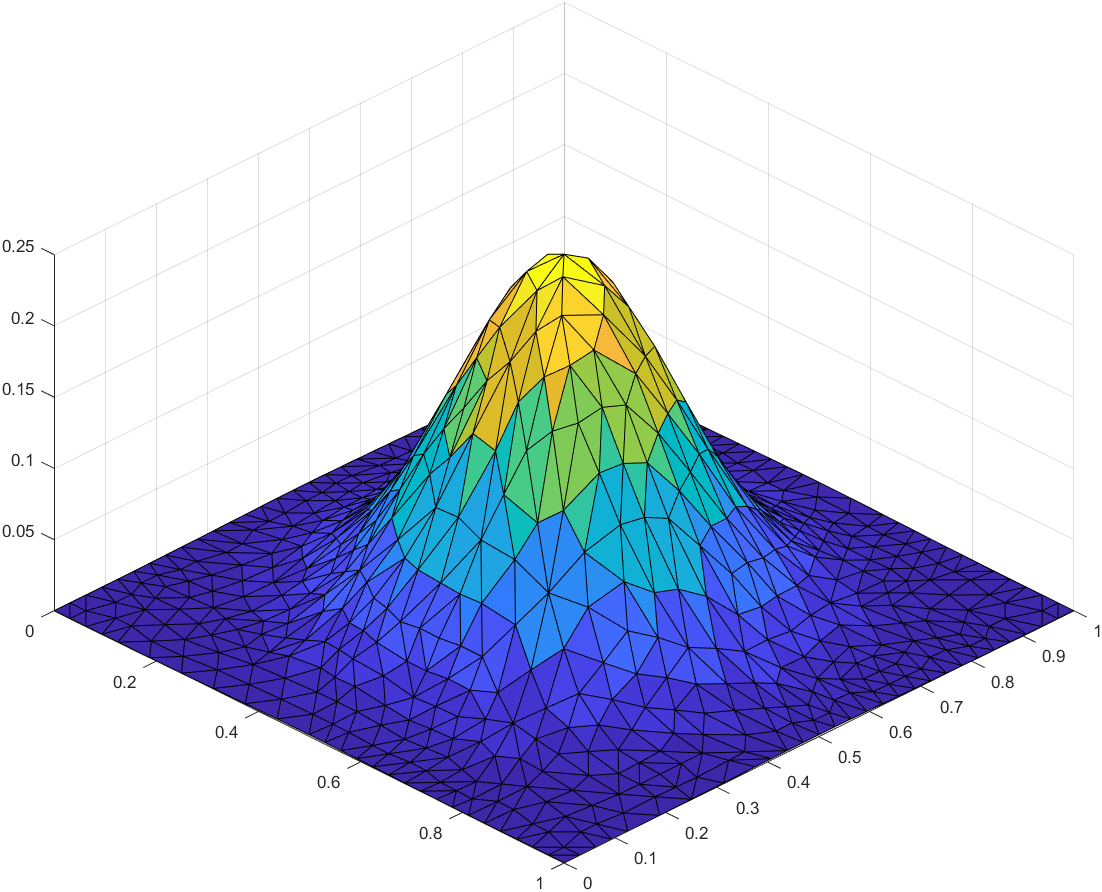
\includegraphics[height=\dimIm]{../Immagini/EGM_P2_AMax=dt=0.005_t=0.5.png}
                            \caption{Tempo $t=0.5$.}
                            \label{figEGMTriangolazioniT5}
                        \end{subfigure}
                        \begin{subfigure}[t]{\lungSF}
                            \centering
                            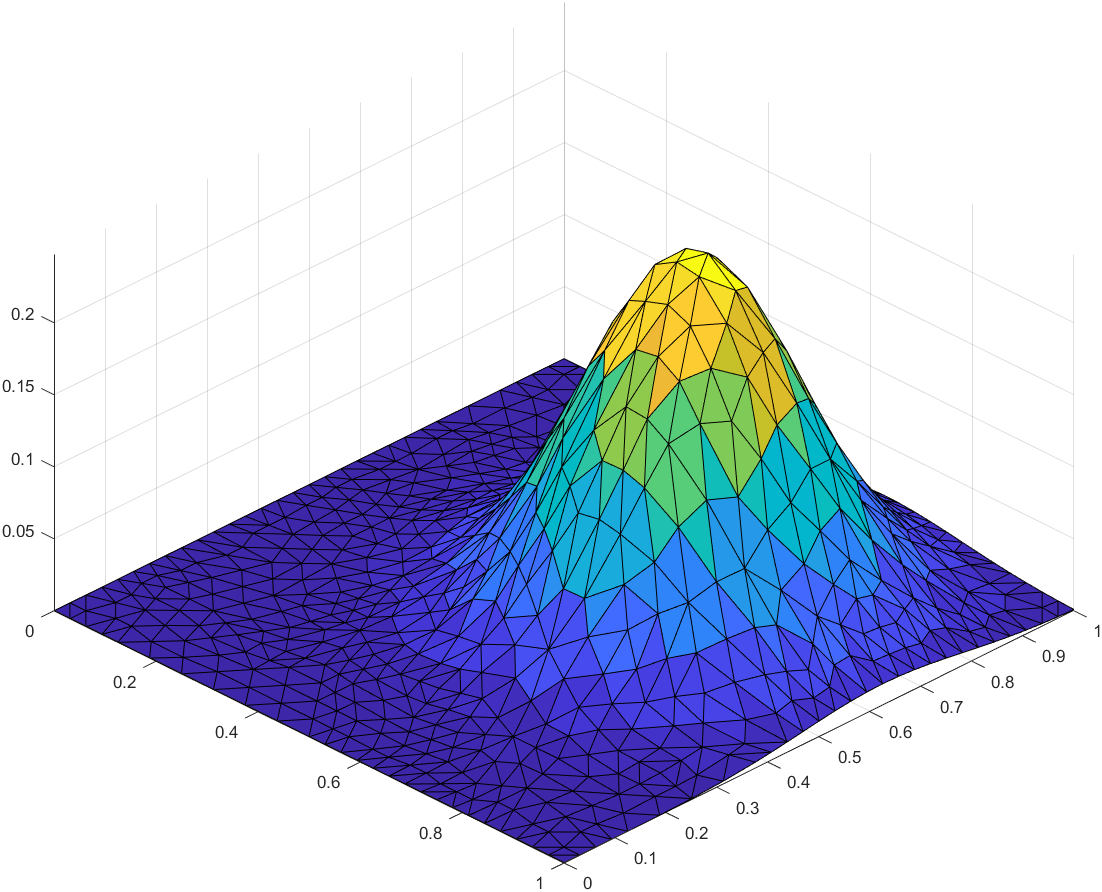
\includegraphics[height=\dimIm]{../Immagini/EGM_P2_AMax=dt=0.005_t=0.625.png}
                            \caption{Tempo $t=0.625$.}
                            \label{figEGMTriangolazioniT6}
                        \end{subfigure}
                    }
                    \distR
                    
                    \makebox[\linewidth][c]{
                        % \captionsetup[subfigure]{width=2.4cm}
                        \SpaziaturaMate{1}{1}{1}
                        \begin{subfigure}[t]{\lungSF}
                            \centering
                            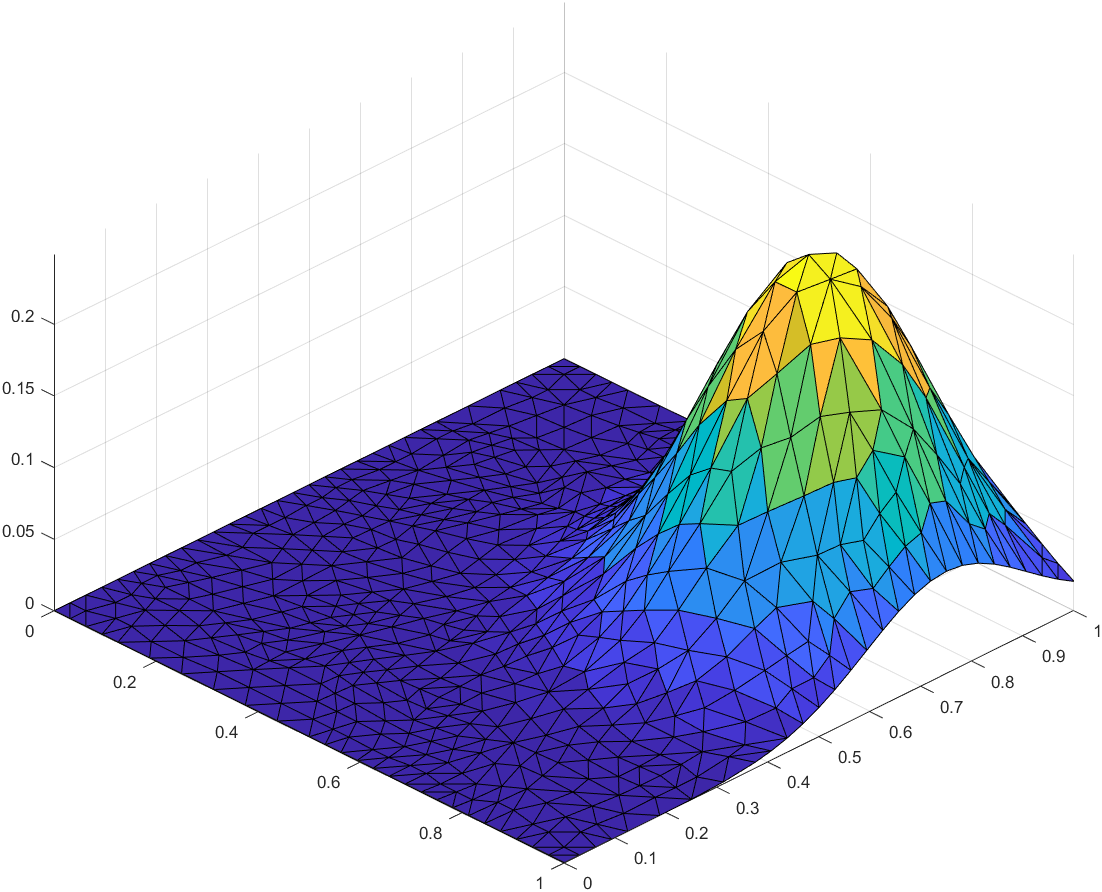
\includegraphics[height=\dimIm]{../Immagini/EGM_P2_AMax=dt=0.005_t=0.75.png}
                            \caption{Tempo $t=0.75$.}
                            \label{figEGMTriangolazioniT7}
                        \end{subfigure}
                        \begin{subfigure}[t]{\lungSF}
                            \centering
                            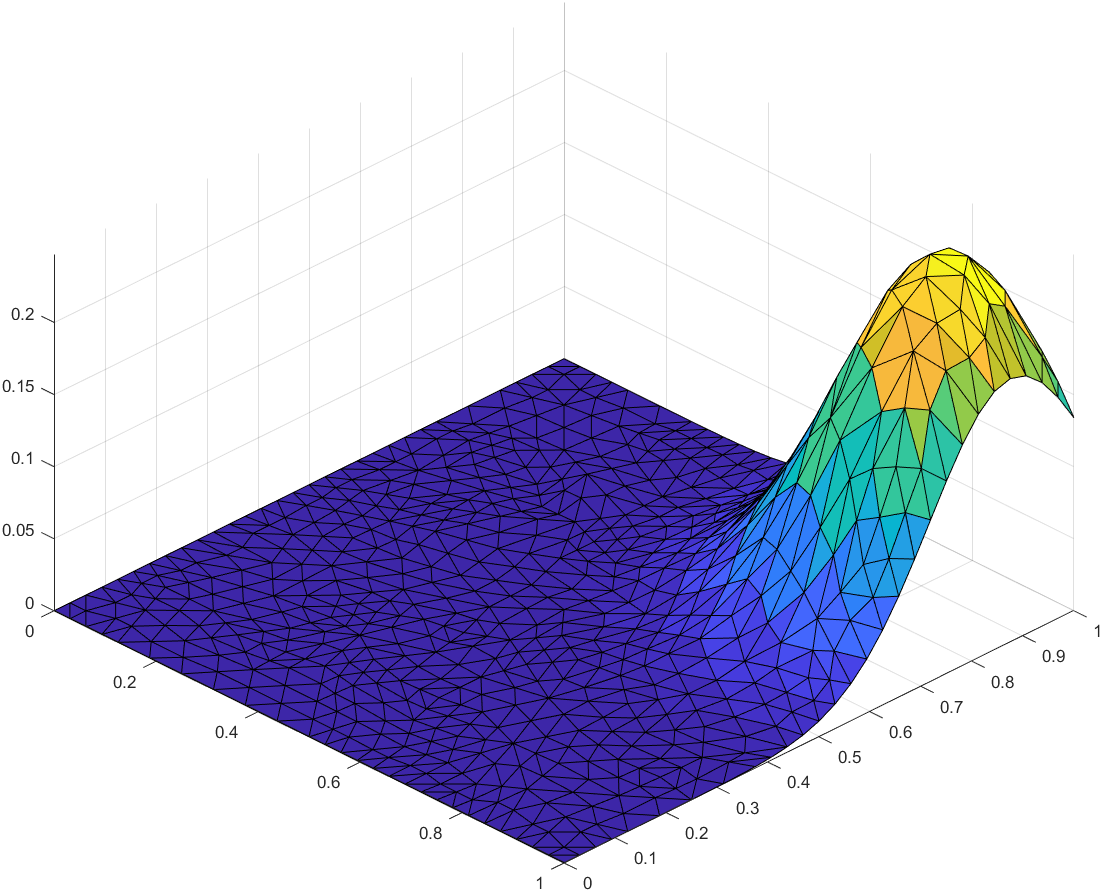
\includegraphics[height=\dimIm]{../Immagini/EGM_P2_AMax=dt=0.005_t=0.875.png}
                            \caption{Tempo $t=0.875$.}
                            \label{figEGMTriangolazioniT8}
                        \end{subfigure}
                        \begin{subfigure}[t]{\lungSF}
                            \centering
                            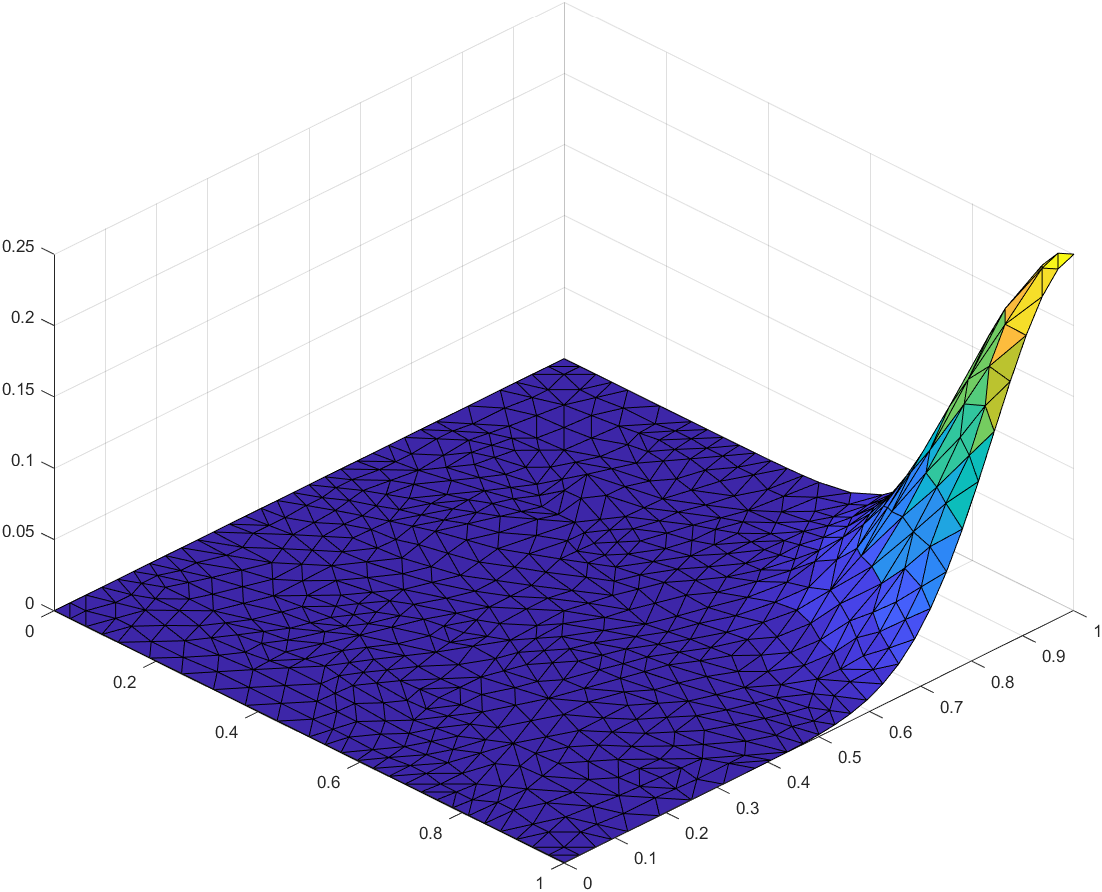
\includegraphics[height=\dimIm]{../Immagini/EGM_P2_AMax=dt=0.005_t=1.png}
                            \caption{Tempo $t=1$.}
                            \label{figEGMTriangolazioniT9}
                        \end{subfigure}
                    }
                   
                    \caption{Soluzione approssimata dell'EGM coi $\mathbb P_2$ in nove istanti evolutivi.}
                    \label{figEGN}
                \end{figure*}
                %%%%%%%%%%%%%%%%%%
                %%%%%%%%%%%%%%%%%%
                %%%%%%%%%%%%%%%%%%
                

            \subsubsection{In tempo \texorpdfstring{$\mathbb P_1$}{P1} (ET1)}
            
                In questo s'impone che la soluzione esatta $u$ del \eqref{eqPETS12} sia pari a
                %
                \begin{equation*}
                    u=g+h=x+y+\sin(5t),
                    \label{eqSoluzioneEsattaET1}
                \end{equation*}
                %
                cosí da verificare l'ordine di convergenza di CN coi $\mathbb P_1$.

                {\SpaziaturaMate{1}{2}{3}
                Nelle Figg. \ref{figET1TriangolazioniEsattaTI}-\ref{figET1TriangolazioniEsattaTF} è mostrata la soluzione esatta in tre istanti di tempo ($t=0,0.5,1$), mentre nelle Figg. \ref{figET1TriangolazioniP1TI}-\ref{figET1TriangolazioniP1TF} le relative approssimazioni mediante i $\mathbb P_1$ e CN. D'altro canto nelle Figg. \ref{figET1ErroreP1Lin} e \ref{figET1ErroreP1Log} è illustrato l'andamento dell'errore per CN (i relativi dati si trovano nella Tab. \ref{tabErroriET1}); questi andamenti corrispondono a quanto detto nel $\S$\ref{parAnalisiErrore}.}
                
            
            \subsubsection{In tempo \texorpdfstring{$\mathbb P_2$}{P2} (ET2)}

                In questo s'impone che la soluzione esatta $u$ del \eqref{eqPETS12} sia pari a
                %
                \begin{equation*}
                    u=g+h=x^2+y^2+\sin(5t)
                    \label{eqSoluzioneEsattaET2}
                \end{equation*}
                %
                cosí da verificare l'ordine di convergenza di CN coi $\mathbb P_2$.

                {\SpaziaturaMate{1}{2}{3}
                Nelle Figg. \ref{figET2TriangolazioniEsattaTI}-\ref{figET2TriangolazioniEsattaTF} è mostrata la soluzione esatta in tre istanti di tempo ($t=0,0.5,1$), mentre nelle Figg. \ref{figET2TriangolazioniP2TI}-\ref{figET2TriangolazioniP2TF} le relative approssimazioni mediante i $\mathbb P_2$ e CN. D'altro canto nelle Figg. \ref{figET2ErroreP2Lin} e \ref{figET2ErroreP2Log} è illustrato l'andamento dell'errore per CN (i relativi dati si trovano nella Tab. \ref{tabErroriET2}); questi andamenti corrispondono a quanto detto nel $\S$\ref{parAnalisiErrore}.}

            
            \subsubsection{In spazio \texorpdfstring{$\mathbb P_1$}{P1} (ES1)}

                In questo s'impone che la soluzione esatta $u$ del \eqref{eqPETS12} sia pari a
                %
                \begin{equation}
                    u=g+h=\sin(x)+y^3+t^2
                    \label{eqSoluzioneEsattaES1}
                \end{equation}
                %
                cosí da verificare l'ordine di convergenza dei $\mathbb P_1$ con CN.

                {\SpaziaturaMate{1}{2}{3}
                Nelle Figg. \ref{figES1TriangolazioniEsattaTI}-\ref{figES1TriangolazioniEsattaTF} è mostrata la soluzione esatta in tre istanti di tempo ($t=0,0.5,1$), mentre nelle Figg. \ref{figES1TriangolazioniP1TI}-\ref{figES1TriangolazioniP1TF} le relative approssimazioni mediante i $\mathbb P_1$ e CN. D'altro canto nelle Figg. \ref{figES1ErroreP1Lin} e \ref{figES1ErroreP1Log} è illustrato l'andamento dell'errore per i $\mathbb P_1$ (i relativi dati si trovano nella Tab. \ref{tabErroriES1}); questi andamenti corrispondono a quanto detto nel $\S$\ref{parAnalisiErrore}.}
                
            
            \subsubsection{In spazio \texorpdfstring{$\mathbb P_2$}{P2} (ES2)}

                In questo s'impone che la soluzione esatta $u$ del \eqref{eqPETS12} sia uguale alla \eqref{eqSoluzioneEsattaES1}, per verificare l'ordine di convergenza dei $\mathbb P_2$ con CN.

                {\SpaziaturaMate{1}{2}{3}
                Nelle Figg. \ref{figES2TriangolazioniEsattaTI}-\ref{figES2TriangolazioniEsattaTF} è mostrata la soluzione esatta in tre istanti di tempo ($t=0,0.5,1$), mentre nelle Figg. \ref{figES2TriangolazioniP2TI}-\ref{figES2TriangolazioniP2TF} le relative approssimazioni mediante i $\mathbb P_2$ e CN. D'altro canto nelle Figg. \ref{figES2ErroreP2Lin} e \ref{figES2ErroreP2Log} è illustrato l'andamento dell'errore per i $\mathbb P_2$ (i relativi dati si trovano nella Tab. \ref{tabErroriES2}); questi andamenti corrispondono a quanto detto nel $\S$\ref{parAnalisiErrore}.}
                

            \subsubsection{Gaussiana movente (EGM)}

                In questo s'impone che la soluzione esatta $u$ del \eqref{eqPETS12} sia pari a
                %
                \begin{equation*}
                    u=N\exp\left(-\frac{(x-t)^2+(y-t)^2}{2\sigma^2}\right)
                    \label{eqSoluzioneEsattaEGM}
                \end{equation*}
                %
                ove $N=0.25$, $\sigma^2=1/40$ e $\mu=t$ da cui il nome del caso di studio: essa è una distribuzione normale che si muove lungo la diagonale nel primo quadrante dall'origine al punto $(1,1)$ nell'intervallo di tempo $[0,1]$.

                {\SpaziaturaMate{1}{2}{3}
                Come già accennato nel $\S$\ref{parProblemaEvolutivoErrori}, l'EGM è solo qualitativo e si limita a mostrare la soluzione approssimata mediante i $\mathbb P_2$ e CN in nove istanti temporali ($t=0,0.125,\ldots,1$)} nella Fig. \ref{figEGN}.

                L'aspetto notevole di questa funzione è che può modellare, sotto altre ipotesi e con piú EDP accoppiate, la chemotassi di cellule, svelando uno spiraglio applicativo molto interessante.

    %%%%%%%%%
    %%%%%%%%%
    %%%%%%%%%
    
    \section{Conclusioni}

        Tutt'i risultati ricavati corrispondono alla teoria studiata; l'unica eccezione è il caso di studio della diffusione-reazione, la cui differenza reputiamo discenda dalla difficoltà a manifestare le instabilità necessarie per giustificare l'ammassamento.

    %%%%%%%%%
    %%%%%%%%%
    %%%%%%%%%
    
    \bibliographystyle{ieeetr}
    \bibliography{Bibliografia}
    \nocite{*} % Include tutti riferimenti bibliografici

\end{document}

% [-+]?\b\d+(\.\d+)?\b
